
\documentclass[twoside,11pt]{article}
\textheight=8.5in
\textwidth=6.5in
\topmargin=-.3in
\oddsidemargin=0in
\evensidemargin=0in
\parskip=6pt plus2pt minus2pt
\pagestyle{headings}

\newlabel{introduction}{{1}{1}}
\newlabel{programs}{{1.1}{1}}
\newlabel{intro-kernel}{{1.2}{2}}
\newlabel{errors}{{1.3}{2}}
\newlabel{namespaces}{{1.4}{2}}
\newlabel{lexical-structure}{{2}{4}}
\newlabel{notational-conventions}{{2.1}{4}}
\newlabel{lexemes}{{2.2}{5}}
\newlabel{whitespace}{{2.2}{5}}
\newlabel{ids}{{2.4}{6}}
\newlabel{lexemes-numeric}{{2.5}{8}}
\newlabel{lexemes-char}{{2.6}{8}}
\newlabel{lexemes-layout}{{2.7}{9}}
\newlabel{layout-before}{{1}{11}}
\newlabel{layout-after}{{2}{11}}
\newlabel{expressions}{{3}{12}}
\newlabel{syntax-precedences}{{1}{13}}
\newlabel{basic-errors}{{3.1}{14}}
\newlabel{applications}{{3.3}{16}}
\newlabel{lambda-abstractions}{{3.3}{16}}
\newlabel{operators}{{3.4}{16}}
\newlabel{sections}{{3.5}{17}}
\newlabel{conditionals}{{3.6}{17}}
\newlabel{lists}{{3.7}{18}}
\newlabel{tuples}{{3.8}{18}}
\newlabel{unit-expression}{{3.9}{18}}
\newlabel{arithmetic-sequences}{{3.10}{19}}
\newlabel{list-comprehensions}{{3.11}{19}}
\newlabel{let-expressions}{{3.12}{21}}
\newlabel{case}{{3.13}{21}}
\newlabel{do-expressions}{{3.14}{22}}
\newlabel{field-ops}{{3.15}{23}}
\newlabel{expression-type-sigs}{{3.16}{25}}
\newlabel{pattern-matching}{{3.17}{26}}
\newlabel{patterns}{{3.17}{26}}
\newlabel{pattern-definitions}{{3.17.1}{26}}
\newlabel{case-semantics}{{3.17.3}{29}}
\newlabel{simple-case-expr-1}{{3}{30}}
\newlabel{simple-case-expr-2}{{4}{31}}
\newlabel{declarations}{{4}{32}}
\newlabel{types-overview}{{4.1}{33}}
\newlabel{type-syntax}{{4.1.1}{34}}
\newlabel{types}{{4.1.1}{34}}
\newlabel{classes&contexts}{{4.1.2}{36}}
\newlabel{type-semantics}{{4.1.3}{36}}
\newlabel{user-defined-datatypes}{{4.2}{37}}
\newlabel{datatype-decls}{{4.2.1}{38}}
\newlabel{field-labels}{{4.2.1}{39}}
\newlabel{strictness-flags}{{4.2.1}{39}}
\newlabel{type-synonym-decls}{{4.2.2}{40}}
\newlabel{datatype-renaming}{{4.2.3}{41}}
\newlabel{overloading}{{4.3}{42}}
\newlabel{classes}{{4.3}{42}}
\newlabel{class-decls}{{4.3.1}{42}}
\newlabel{instance-decls}{{4.3.2}{43}}
\newlabel{derived-decls}{{4.3.3}{45}}
\newlabel{default-decls}{{4.3.4}{45}}
\newlabel{nested}{{4.4}{47}}
\newlabel{type-signatures}{{4.4.1}{47}}
\newlabel{function-bindings}{{4.4.2}{48}}
\newlabel{pattern-bindings}{{4.4.2}{48}}
\newlabel{dependencyanalysis}{{4.5}{50}}
\newlabel{generalization}{{4.5.2}{51}}
\newlabel{context-reduction}{{4.5.3}{52}}
\newlabel{monomorphism}{{4.5.4}{52}}
\newlabel{sect:monomorphism-restriction}{{4.5.5}{53}}
\newlabel{kindinference}{{4.6}{56}}
\newlabel{modules}{{5}{57}}
\newlabel{module-implementations}{{5.1}{57}}
\newlabel{export}{{5.2}{58}}
\newlabel{import}{{5.3}{59}}
\newlabel{as-clause}{{5.3.2}{61}}
\newlabel{qualifiers}{{5.5.1}{61}}
\newlabel{closure}{{5.5.3}{63}}
\newlabel{standard-prelude}{{5.6}{64}}
\newlabel{std-prel-shadowing}{{5.6.2}{65}}
\newlabel{abstract-types}{{5.8}{66}}
\newlabel{fixity}{{5.9}{66}}
\newlabel{prelude-fixities}{{2}{67}}
\newlabel{basic-types-and-classes}{{6}{68}}
\newlabel{basic-types}{{6.1}{68}}
\newlabel{booleans}{{6.1.1}{68}}
\newlabel{prelude-bool}{{6.1.1}{68}}
\newlabel{characters}{{6.1.2}{68}}
\newlabel{basic-lists}{{6.1.3}{69}}
\newlabel{basic-tuples}{{6.1.4}{69}}
\newlabel{basic-trivial}{{6.1.5}{69}}
\newlabel{strict-eval}{{6.2}{70}}
\newlabel{standard-classes}{{5}{72}}
\newlabel{monad-class}{{6.3.6}{76}}
\newlabel{numbers}{{6.4}{77}}
\newlabel{numeric-literals}{{6.4.1}{77}}
\newlabel{standard-numeric-types}{{3}{78}}
\newlabel{arithmetic-operators}{{6.4.2}{78}}
\newlabel{basic-numeric-1}{{6}{79}}
\newlabel{magnitude-sign}{{6.4.4}{79}}
\newlabel{basic-numeric-2}{{7}{80}}
\newlabel{coercion}{{6.4.6}{81}}
\newlabel{io}{{7}{83}}
\newlabel{stdprelude}{{A}{87}}
\newlabel{preludelist}{{A.1}{101}}
\newlabel{preludetext}{{A.2}{108}}
\newlabel{preludeio}{{A.3}{113}}
\newlabel{syntax}{{B}{115}}
\newlabel{layout}{{B.3}{118}}
\newlabel{bnf}{{B.4}{121}}
\newlabel{literate}{{C}{126}}
\newlabel{derived-appendix}{{D}{128}}
\newlabel{tree-inst}{{8}{132}}
\newlabel{pragmas}{{E}{133}}


\usepackage{epsf}

% \renewcommand{\thepage}{T-\arabic{page}}

\newcommand{\folks}[1]{\begin{quote}\sf#1\end{quote}}
\newcommand{\bc}{\begin{center}}
\newcommand{\ec}{\end{center}}
\newcommand{\be}{\begin{enumerate}}
\newcommand{\ee}{\end{enumerate}}
\newcommand{\ba}{\begin{array}}
\newcommand{\ea}{\end{array}}
\newcommand{\x}{\times}
\newcommand{\lam}{\lambda}
\newcommand{\la}{\leftarrow}
\newcommand{\ra}{\rightarrow}
\newcommand{\red}{\Rightarrow}
\newcommand{\see}[1]{\S\ref{#1}}
\newcommand{\syn}[1]{[#1]}
\newcommand{\bprog}{%
\par\noindent\begin{tabular}{@{\hspace*{17pt}}l@{}}}
\newcommand{\eprog}{%
\end{tabular}\\[\parskip]}
\newcommand{\eprogNoSkip}{%
\end{tabular}}

\newcommand{\anchor}[2]{#2}

\begin{document}

\title{A Gentle Introduction to Haskell 98}
\author{Paul Hudak\\
Yale University\\
Department of Computer Science  
\and
John Peterson\\
Yale University\\
Department of Computer Science  
\and
Joseph H. Fasel\\
University of California\\
Los Alamos National Laboratory}
\date{October, 1999}

\maketitle

Copyright \copyright\ 1999 Paul Hudak, John Peterson and Joseph Fasel

     Permission is hereby granted, free of charge, to any person obtaining
     a copy of ``A Gentle Introduction to Haskell'' (the Text), to deal
     in the Text without restriction, including without limitation the
     rights to use, copy, modify, merge, publish, distribute, sublicense,
     and/or sell copies of the Text, and to permit persons to whom the
     Text is furnished to do so, subject to the following condition:
     The above copyright notice and this permission notice shall be
     included in all copies or substantial portions of the Text.


%**<title>A Gentle Introduction to Haskell: Introduction</title>
%**~sheader

\section{Introduction}
\label{tut-intro}

Our purpose in writing this tutorial is not to teach programming, nor
even to teach functional programming.  Rather, it is intended to serve
as a supplement to the Haskell Report \cite{haskell-98}, which is
otherwise a rather dense technical exposition.  Our goal is to provide
a gentle introduction to Haskell for someone who has experience with
at least one other language, preferably a functional language (even if
only an ``almost-functional'' language such as ML or Scheme).
If the
reader wishes to learn more about the functional programming style, we
highly recommend Bird's text {\em Introduction to
Functional Programming} \cite{bird98} or Davie's {\em An Introduction
to Functional Programming Systems Using Haskell} \cite{davie92}. 
For a useful survey of functional programming languages
and techniques, including some of the language design principles used
in Haskell, see \cite{huda89a}.

The Haskell language has evolved significantly since its birth in 1987.
This tutorial deals with \anchor{http://haskell.org/report}
{Haskell 98}.  Older versions of the language are now obsolete;
Haskell users are encouraged to use Haskell 98.  There are also many
extensions to Haskell 98 that have been widely implemented.  These are
not yet a formal part of the Haskell language and are not covered in
this tutorial.

Our general strategy for introducing language features is this:
motivate the idea, define some terms, give some examples, and then
point to the Report for details.  We suggest, however, that the reader
completely ignore the details until the {\em Gentle Introduction} has been
completely read.  On the other hand, Haskell's Standard Prelude (in
Appendix A of the Report and the standard libraries
(found in the \anchor{http://haskell.org/library}
Library Report~\cite{haskell-libs}) contain
lots of useful examples of Haskell code; we 
encourage a thorough reading once this tutorial is completed.  This
will not only give the reader a feel for what real Haskell code looks
like, but will also familiarize her with Haskell's standard set of
predefined functions and types.

Finally, the Haskell web site, \anchor{http://haskell.org}{{\tt
http://haskell.org}}, has a wealth of information about the Haskell
language and its implementations.  


\syn{We have also taken the course of not laying out a plethora of
lexical syntax rules at the outset.  Rather, we introduce them
incrementally as our examples demand, and enclose them in brackets, as
with this paragraph.  This is in stark contrast to the organization of
the Report, although the Report remains the authoritative source for
details (references such as ``\S 2.1'' refer to sections in the
Report).}

Haskell is a {\em typeful} programming language:\footnote{Coined by Luca Cardelli.} types are pervasive, and the newcomer is best off
becoming well aware of the full power and complexity of Haskell's type
system from the outset.  For those whose only experience is with
relatively ``untypeful'' languages such as Perl, Tcl, or Scheme, this may be
a difficult adjustment; for those familiar with Java, C, Modula, or
even ML, the adjustment should be easier but still not insignificant,
since Haskell's type system is different and somewhat richer than
most.  In any case, ``typeful programming'' is part of the Haskell
programming experience, and cannot be avoided.

% \maybeInclude{intro-extra}

%**~sfooter

%**<title>A Gentle Introduction to Haskell: Values and Types</title>

%**~header

\section{Values, Types, and Other Goodies}
\label{tut-values-etc}

Because Haskell is a purely functional language, all computations are
done via the evaluation of {\em expressions} (syntactic terms) to
yield {\em values} (abstract entities that we regard as answers).
Every value has an associated 
{\em type}.  (Intuitively, we can think of types as sets of values.)
Examples of expressions include atomic values such as the integer \mbox{\tt 5},
the character \mbox{\tt 'a'}, and the function \mbox{\tt {\char'134}x\ ->\ x+1}, as well as
structured values such as the list \mbox{\tt [1,2,3]} and the pair \mbox{\tt ('b',4)}.

Just as expressions denote values, type expressions are
syntactic terms that denote type values (or just {\em types}).
Examples of type expressions include the atomic types \mbox{\tt Integer}
(infinite-precision integers), \mbox{\tt Char} (characters), \mbox{\tt Integer->Integer}
(functions mapping \mbox{\tt Integer} to \mbox{\tt Integer}), as well as the structured types
\mbox{\tt [Integer]} (homogeneous lists of integers) and \mbox{\tt (Char,Integer)}
(character, integer pairs).

All Haskell values are ``first-class''---they may be passed as
arguments to functions, returned as results, placed in data
structures, etc.  Haskell types, on the other hand, are {\em not}
first-class.  Types in a sense describe values, and the
association of a value with its type is called a {\em typing}.  Using
the examples of values and types above, we write typings as follows:
\bprog
\mbox{\tt \ \ \ \ \ \ \ \ \ \ \ \ \ \ \ \ \ \ \ \ \ \ \ \ \ \ 5\ \ ::\ Integer}\\
\mbox{\tt \ \ \ \ \ \ \ \ \ \ \ \ \ \ \ \ \ \ \ \ \ \ \ \ \ 'a'\ ::\ Char}\\
\mbox{\tt \ \ \ \ \ \ \ \ \ \ \ \ \ \ \ \ \ \ \ \ \ \ \ \ \ inc\ ::\ Integer\ ->\ Integer}\\
\mbox{\tt \ \ \ \ \ \ \ \ \ \ \ \ \ \ \ \ \ \ \ \ \ [1,2,3]\ ::\ [Integer]}\\
\mbox{\tt \ \ \ \ \ \ \ \ \ \ \ \ \ \ \ \ \ \ \ \ \ ('b',4)\ ::\ (Char,Integer)}
\eprog
The ``\mbox{\tt ::}'' can be read ``has type.''

Functions in Haskell are normally defined by a series of {\em
equations}.  For example, the function \mbox{\tt inc} can be
defined by the single equation:
\bprog
\mbox{\tt inc\ n\ \ \ \ \ \ \ \ \ \ =\ n+1}
\eprog 
An equation is an example of a {\em declaration}.  Another kind of
declaration is a {\em type signature declaration}
(\see{type-signatures}), with which we can declare an explicit typing
for \mbox{\tt inc}:
\bprog
\mbox{\tt inc\ \ \ \ \ \ \ \ \ \ \ \ ::\ Integer\ ->\ Integer}
\eprog 
We will have much more to say about function definitions in Section
\ref{tut-functions}.

For pedagogical purposes, when we wish to indicate that an expression
$e_1$ evaluates, or ``reduces,'' to another expression or value $e_2$,
we will write:
\[ e_1\ \ \ \ \red\ \ \ \ e_2 \]
For example, note that:
\[ \mbox{\tt inc\ (inc\ 3)}\ \ \ \ \red\ \ \ \ \mbox{\tt 5} \]

Haskell's static type system defines the formal relationship
between types and values (\see{type-semantics}).  The static type
system ensures that Haskell programs are {\em type safe}; that is,
that the programmer has not mismatched types in some way.  For
example, we cannot generally add together two characters, so the
expression \mbox{\tt 'a'+'b'} is ill-typed.  The main advantage of statically
typed languages is well-known: All type errors are detected at
compile-time.  Not all errors are caught by the type system; an
expression such as \mbox{\tt 1/0} is typable but its evaluation will result in
an error at execution time.  Still, the type system finds many
program errors at compile time, aids the user in reasoning about
programs, and also permits a compiler to generate more efficient code
(for example, no run-time type tags or tests are required).

The type system also ensures that user-supplied type signatures are
correct.  In fact, Haskell's type system is powerful enough to allow
us to avoid writing any type signatures at all;\footnote{With a few
exceptions to be described later.} we say that the type
system {\em infers} the correct types for us.  Nevertheless, judicious
placement of type signatures such as that we gave for \mbox{\tt inc} is a good idea,
since type signatures are a very effective form of documentation and
help bring programming errors to light.

\syn{The reader will note that we have capitalized identifiers that
denote specific types, such as \mbox{\tt Integer} and \mbox{\tt Char}, but not identifiers
that denote values, such as \mbox{\tt inc}.  This is not just a convention: it
is enforced by Haskell's lexical syntax.  In fact, the case of the
other characters matters, too: \mbox{\tt foo}, \mbox{\tt fOo}, and \mbox{\tt fOO} are all
distinct identifiers.}

\subsection{Polymorphic Types}
\label{tut-polymorphism}

Haskell also incorporates {\em polymorphic} types---types that are
universally quantified in some way over all types.  Polymorphic
type expressions essentially describe families of types.  For
example, $(\forall$\mbox{\tt a}$)$\mbox{\tt [a]} is the family of types consisting of,
for every type \mbox{\tt a}, the type of lists of \mbox{\tt a}.  Lists of integers
(e.g.~\mbox{\tt [1,2,3]}), lists of characters (\mbox{\tt ['a','b','c']}), even lists of
lists of integers, etc., are all members of this family.  (Note,
however, that \mbox{\tt [2,'b']} is {\em not} a valid example, since there is
no single type that contains both \mbox{\tt 2} and \mbox{\tt 'b'}.)

\syn{Identifiers such as \mbox{\tt a} above are called {\em type variables},
and are uncapitalized to distinguish them from specific types such as
\mbox{\tt Int}.  Furthermore, since Haskell has only universally quantified
types, there is no need to explicitly write out the symbol for
universal quantification, and thus we simply write \mbox{\tt [a]} in the
example above.  In other words, all type variables are implicitly
universally quantified.}

Lists are a commonly used data structure in functional languages, and
are a good vehicle for explaining the principles of polymorphism.  The
list \mbox{\tt [1,2,3]} in Haskell is actually shorthand for the list
\mbox{\tt 1:(2:(3:[]))}, where \mbox{\tt []} is the empty list and \mbox{\tt :} is the infix
operator that adds its first argument to the front of its second
argument (a list).\footnote{\mbox{\tt :} and \mbox{\tt []} are like Lisp's \mbox{\tt cons} and
\mbox{\tt nil}, respectively.} Since \mbox{\tt :} is right associative, we can also
write this list as \mbox{\tt 1:2:3:[]}.

As an example of a user-defined function that operates on lists,
consider the problem of counting the number of elements in a list:
\bprog
\mbox{\tt length\ \ \ \ \ \ \ \ \ \ \ \ \ \ \ \ \ \ ::\ [a]\ ->\ Integer}\\
\mbox{\tt length\ []\ \ \ \ \ \ \ \ \ \ \ \ \ \ \ =\ \ 0}\\
\mbox{\tt length\ (x:xs)\ \ \ \ \ \ \ \ \ \ \ =\ \ 1\ +\ length\ xs}
\eprog 
This definition is almost self-explanatory.  We can read the equations
as saying: ``The length of the empty list is 0, and the length of a
list whose first element is \mbox{\tt x} and remainder is \mbox{\tt xs} is 1 plus the
length of \mbox{\tt xs}.'' (Note the naming convention used here; \mbox{\tt xs} is the
plural of \mbox{\tt x}, and should be read that way.)

Although intuitive, this example highlights an important aspect of
Haskell that is yet to be explained: {\em pattern matching}.  The
left-hand sides of the equations contain patterns such as \mbox{\tt []}
and \mbox{\tt x:xs}.  In a function application these patterns are 
matched against actual parameters in a fairly intuitive way (\mbox{\tt []}
only matches the empty list, and \mbox{\tt x:xs} will successfully match any
list with at least one element, binding \mbox{\tt x} to the first element and
\mbox{\tt xs} to the rest of the list).  If the match succeeds, the right-hand
side is evaluated and returned as the result of the application.  If
it fails, the next equation is tried, and if all equations fail, an
error results.

Defining functions by pattern matching is quite common in Haskell, and
the user should become familiar with the various kinds of patterns
that are allowed; we will return to this issue in
Section~\ref{tut-pattern-matching}. 

The \mbox{\tt length} function is also an example of a polymorphic
function.  It can 
be applied to a list containing elements of any type, for example
\mbox{\tt [Integer]}, \mbox{\tt [Char]}, or \mbox{\tt [[Integer]]}.
\[\ba{lcl}
  \mbox{\tt length\ [1,2,3]}      &\ \ \ \ \red\ \ \ \ & 3\\
  \mbox{\tt length\ ['a','b','c']}&\ \ \ \ \red\ \ \ \ & 3\\
  \mbox{\tt length\ [[1],[2],[3]]}   &\ \ \ \ \red\ \ \ \ & 3
\ea\]

Here are two other useful polymorphic functions on lists that will be
used later.  Function \mbox{\tt head} returns the first element of a list,
function \mbox{\tt tail} returns all but the first.
\bprog
\mbox{\tt head\ \ \ \ \ \ \ \ \ \ \ \ \ \ \ \ \ \ \ \ ::\ [a]\ ->\ a}\\
\mbox{\tt head\ (x:xs)\ \ \ \ \ \ \ \ \ \ \ \ \ =\ \ x}\\
\mbox{\tt }\\[-8pt]
\mbox{\tt tail\ \ \ \ \ \ \ \ \ \ \ \ \ \ \ \ \ \ \ \ ::\ [a]\ ->\ [a]}\\
\mbox{\tt tail\ (x:xs)\ \ \ \ \ \ \ \ \ \ \ \ \ =\ \ xs}
\eprog 
Unlike \mbox{\tt length}, these functions are not defined for all possible
values of their argument.  A runtime error occurs when these functions
are applied to an empty list.  

With polymorphic types, we find that some types are in a sense
strictly more general than others in the sense that the set of
values they define is larger.  For example, the type \mbox{\tt [a]}
is more general than \mbox{\tt [Char]}.  In other words, the latter type can be
derived from the former by a suitable substitution for \mbox{\tt a}.  With
regard to this generalization ordering, Haskell's type system
possesses two important properties: First, every well-typed expression
is guaranteed to have a unique principal type (explained below),
and second, the principal type can be inferred automatically
(\see{type-semantics}).  In comparison to a monomorphically
typed language such as C, the reader will find that 
polymorphism improves expressiveness, and type inference
lessens the burden of types on the programmer.

An expression's or function's principal type is the least general type
that, intuitively, ``contains all instances of the expression''.  For
example, the principal type of \mbox{\tt head} is \mbox{\tt [a]->a}; \mbox{\tt [b]->a},
\mbox{\tt a->a}, or even \mbox{\tt a} are correct types, but too general, whereas something
like \mbox{\tt [Integer]->Integer} is too specific.  The existence of unique principal
types is the hallmark feature of the {\em Hindley-Milner type system},
which forms the basis of the type systems of Haskell, ML,
Miranda,\footnote{``Miranda'' is a trademark of Research Software,
Ltd.} and several other (mostly functional) languages.

\subsection{User-Defined Types}
\label{tut-user-types}

We can define our own types in Haskell using a \mbox{\tt data} declaration,
which we introduce via a series of examples (\see{datatype-decls}).

An important predefined type in Haskell is that of truth values:
\bprog
\mbox{\tt data\ Bool\ \ \ \ \ \ \ \ \ \ \ \ \ \ \ =\ False\ |\ True}
\eprog
The type being defined here is \mbox{\tt Bool}, and it has exactly two values:
\mbox{\tt True} and \mbox{\tt False}.  Type \mbox{\tt Bool} is an example of a (nullary) {\em type
constructor}, and \mbox{\tt True} and \mbox{\tt False} are (also nullary) {\em data
constructors} (or just {\em constructors}, for short).

Similarly, we might wish to define a color type:
\bprog
\mbox{\tt data\ Color\ \ \ \ \ \ \ \ \ \ \ \ \ \ =\ Red\ |\ Green\ |\ Blue\ |\ Indigo\ |\ Violet}
\eprog
Both \mbox{\tt Bool} and \mbox{\tt Color} are examples of enumerated types, since
they consist of a finite number of nullary data constructors.

Here is an example of a type with just one data constructor:
\bprog
\mbox{\tt data\ Point\ a\ \ \ \ \ \ \ \ \ \ \ \ =\ Pt\ a\ a}
\eprog
Because of the single constructor, a type like \mbox{\tt Point} is often
called a {\em tuple type}, since it is essentially just a cartesian
product (in this case binary) of other types.\footnote{Tuples are
somewhat like records in other languages.}
In contrast, multi-constructor types, such as \mbox{\tt Bool} and
\mbox{\tt Color}, are called (disjoint) union or sum types.

More importantly, however, \mbox{\tt Point} is an example of a 
polymorphic type: for any type $t$, it defines the type of cartesian
points that use $t$ as the coordinate type.  The \mbox{\tt Point} type can now be seen
clearly as a unary type constructor, since from the type $t$ it
constructs a new type \mbox{\tt Point\ }$t$.  (In the same sense, using the list
example given earlier, \mbox{\tt []} is also a type constructor.  Given any type $t$
we can ``apply'' \mbox{\tt []} to yield a new type \mbox{\tt [}$t$\mbox{\tt ]}.  The Haskell
syntax allows \mbox{\tt []\ }$t$ to be written as \mbox{\tt [}$t$\mbox{\tt ]}.  Similarly,
\mbox{\tt ->} is a type constructor: given two types $t$ and $u$,
$t$\mbox{\tt ->}$u$ is the type of functions mapping elements of type $t$ to
elements of type $u$.)

Note that the type of the binary data constructor \mbox{\tt Pt} is \mbox{\tt a\ ->\ a\ ->\ Point\ a}, 
and thus the following typings are valid:
\bprog
\mbox{\tt Pt\ \ 2.0\ \ 3.0\ \ \ \ \ \ \ \ \ \ \ \ ::\ Point\ Float}\\
\mbox{\tt Pt\ \ 'a'\ \ 'b'\ \ \ \ \ \ \ \ \ \ \ \ ::\ Point\ Char}\\
\mbox{\tt Pt\ True\ False\ \ \ \ \ \ \ \ \ \ \ ::\ Point\ Bool}
\eprog
On the other hand, an expression such as \mbox{\tt Pt\ 'a'\ 1} is ill-typed
because \mbox{\tt 'a'} and \mbox{\tt 1} are of different types.

It is important to distinguish between applying a {\em data constructor} to
yield a {\em value}, and applying a {\em type constructor} to yield a
{\em type}; the former happens at run-time and is how we compute
things in Haskell, whereas the latter happens at compile-time and is
part of the type system's process of ensuring type safety.

\syn{Type constructors such as \mbox{\tt Point} and data constructors such as
\mbox{\tt Pt} are in separate namespaces.  This allows the same name to be used
for both a type constructor and data constructor, as in the following:
\bprog
\mbox{\tt data\ Point\ a\ =\ Point\ a\ a}
\eprog
While this may seem a little confusing at first, it serves to make the
link between a type and its data constructor more obvious.}

\subsubsection{Recursive Types}
\label{tut-recursive-types}

Types can also be recursive, as in the type of binary trees:
\bprog
\mbox{\tt data\ Tree\ a\ \ \ \ \ \ \ \ \ \ \ \ \ =\ Leaf\ a\ |\ Branch\ (Tree\ a)\ (Tree\ a)\ }
\eprog
Here we have defined a polymorphic binary tree type whose elements
are either leaf nodes containing a value of type \mbox{\tt a}, or internal
nodes (``branches'') containing (recursively) two sub-trees.

When reading data declarations such as this, remember again that \mbox{\tt Tree} is a
type constructor, whereas \mbox{\tt Branch} and \mbox{\tt Leaf} are data constructors.
Aside from establishing a connection between these constructors, the
above declaration is essentially defining the following types for
\mbox{\tt Branch} and \mbox{\tt Leaf}:
\bprog
\mbox{\tt Branch\ \ \ \ \ \ \ \ \ \ \ \ \ \ \ \ \ \ ::\ Tree\ a\ ->\ Tree\ a\ ->\ Tree\ a}\\
\mbox{\tt Leaf\ \ \ \ \ \ \ \ \ \ \ \ \ \ \ \ \ \ \ \ ::\ a\ ->\ Tree\ a}
\eprog 

With this example we have defined a type sufficiently rich to
allow defining some interesting (recursive) functions that use it.
For example, suppose we wish to define a function \mbox{\tt fringe} that
returns a list of all the elements in the leaves of a tree from left
to right.  It's usually helpful to write down the type of new
functions first; in this case we see that the type should be 
\mbox{\tt Tree\ a\ ->\ [a]}.  That is, \mbox{\tt fringe} is a polymorphic function that,
for any type \mbox{\tt a}, maps trees of \mbox{\tt a} into lists of \mbox{\tt a}.  A suitable
definition follows:
\bprog
\mbox{\tt fringe\ \ \ \ \ \ \ \ \ \ \ \ \ \ \ \ \ \ \ \ \ ::\ Tree\ a\ ->\ [a]}\\
\mbox{\tt fringe\ (Leaf\ x)\ \ \ \ \ \ \ \ \ \ \ \ =\ \ [x]}\\
\mbox{\tt fringe\ (Branch\ left\ right)\ =\ \ fringe\ left\ ++\ fringe\ right}
\eprog
Here \mbox{\tt ++} is the infix operator that concatenates two lists (its full
definition will be given in Section \ref{tut-monadic-classes}).  As
with the \mbox{\tt length} example given earlier, the \mbox{\tt fringe} function is
defined using pattern matching, except that here we see patterns involving
user-defined constructors: \mbox{\tt Leaf} and \mbox{\tt Branch}.  \syn{Note that the
formal parameters are easily identified as the ones beginning with
lower-case letters.}


\subsection{Type Synonyms}
\label{tut-type-synonyms}

For convenience, Haskell provides a way to define {\em type synonyms};
i.e.~names for commonly used types.  Type synonyms are created using a
\mbox{\tt type} declaration (\see{type-synonym-decls}).  Here are several
examples:
\bprog
\mbox{\tt type\ String\ \ \ \ \ \ \ \ \ \ \ \ \ =\ [Char]}\\
\mbox{\tt type\ Person\ \ \ \ \ \ \ \ \ \ \ \ \ =\ (Name,Address)}\\
\mbox{\tt type\ Name\ \ \ \ \ \ \ \ \ \ \ \ \ \ \ =\ String}\\
\mbox{\tt data\ Address\ \ \ \ \ \ \ \ \ \ \ \ =\ None\ |\ Addr\ String}
\eprog

Type synonyms do not define new types, but simply give new names
for existing types.  For example, the type \mbox{\tt Person\ ->\ Name} is
precisely equivalent to \mbox{\tt (String,Address)\ ->\ String}.  The new names
are often shorter than the types they are synonymous with, but this is
not the only purpose of type synonyms: they can also improve
readability of programs by being more mnemonic; indeed, the above
examples highlight this.  We can even give new names to polymorphic
types:
\bprog
\mbox{\tt type\ AssocList\ a\ b\ \ \ \ \ \ \ \ \ \ \ \ \ \ =\ [(a,b)]}
\eprog 
This is the type of ``association lists'' which associate values of
type \mbox{\tt a} with those of type \mbox{\tt b}.

\subsection{Built-in Types Are Not Special}
\label{tut-built-ins}

Earlier we introduced several ``built-in'' types such as lists,
tuples, integers, and characters.  We have also shown how new
user-defined types can be defined.  Aside from special syntax, are
the built-in types in any way more special than the user-defined ones?
The answer is {\em no}.  The special syntax is for convenience and for
consistency with historical convention, but has no semantic
consequences.

We can emphasize this point by considering what the type
declarations would look like for these built-in types if in fact we
were allowed to use the special syntax in defining them.  For example,
the \mbox{\tt Char} type might be written as:
\bprog
\mbox{\tt data\ Char\ \ \ \ \ \ \ =\ 'a'\ |\ 'b'\ |\ 'c'\ |\ ...\ \ \ \ \ \ \ \ \ --\ This\ is\ not\ valid}\\
\mbox{\tt \ \ \ \ \ \ \ \ \ \ \ \ \ \ \ \ |\ 'A'\ |\ 'B'\ |\ 'C'\ |\ ...\ \ \ \ \ \ \ \ \ --\ Haskell\ code!}\\
\mbox{\tt \ \ \ \ \ \ \ \ \ \ \ \ \ \ \ \ |\ '1'\ |\ '2'\ |\ '3'\ |\ ...}\\
\mbox{\tt \ \ \ \ \ \ \ \ \ \ \ \ \ \ \ \ ...}
\eprog
These constructor names are not syntactically valid; to fix them we
would have to write something like:
\bprog
\mbox{\tt data\ Char\ \ \ \ \ \ \ =\ Ca\ |\ Cb\ |\ Cc\ |\ ...}\\
\mbox{\tt \ \ \ \ \ \ \ \ \ \ \ \ \ \ \ \ |\ CA\ |\ CB\ |\ CC\ |\ ...}\\
\mbox{\tt \ \ \ \ \ \ \ \ \ \ \ \ \ \ \ \ |\ C1\ |\ C2\ |\ C3\ |\ ...}\\
\mbox{\tt \ \ \ \ \ \ \ \ \ \ \ \ \ \ \ \ ...}
\eprog
Even though these constructors are more concise, they are quite
unconventional for representing characters.

In any case, writing ``pseudo-Haskell'' code in this way helps us to
see through the special syntax.  We see now that \mbox{\tt Char} is just an
enumerated type consisting of a large number of nullary constructors.
Thinking of \mbox{\tt Char} in this way makes it clear that we can
pattern-match against characters in function definitions, just as we
would expect to be able to do so for any of a type's constructors.

\syn{This example also demonstrates the use of {\em comments} in
Haskell; the characters \mbox{\tt --} and all subsequent characters to the end
of the line are ignored.  Haskell also permits {\em nested} comments
which have the form \mbox{\tt {\char'173}-}$\ldots$\mbox{\tt -{\char'175}} and can appear anywhere
(\see{lexemes}).}

Similarly, we could define \mbox{\tt Int} (fixed precision integers) and
\mbox{\tt Integer} by: 
\bprog
\mbox{\tt data\ Int\ \ \ \ \ =\ -65532\ |\ ...\ |\ -1\ |\ 0\ |\ 1\ |\ ...\ |\ 65532\ \ --\ more\ pseudo-code}\\
\mbox{\tt data\ Integer\ =\ \ \ \ \ \ \ ...\ -2\ |\ -1\ |\ 0\ |\ 1\ |\ 2\ ...}
\eprog
where \mbox{\tt -65532} and \mbox{\tt 65532}, say, are the maximum and minimum fixed
precision integers for a given implementation.  \mbox{\tt Int} is a much larger
enumeration than \mbox{\tt Char}, but it's still finite!  In contrast, the
pseudo-code for \mbox{\tt Integer} 
is intended to convey an {\em infinite} enumeration.

Tuples are also easy to define playing this game:
\bprog
\mbox{\tt data\ (a,b)\ \ \ \ \ \ \ \ \ \ \ \ \ \ =\ (a,b)\ \ \ \ \ \ \ \ \ \ \ \ \ \ \ \ \ \ \ \ \ \ \ \ \ --\ more\ pseudo-code}\\
\mbox{\tt data\ (a,b,c)\ \ \ \ \ \ \ \ \ \ \ \ =\ (a,b,c)}\\
\mbox{\tt data\ (a,b,c,d)\ \ \ \ \ \ \ \ \ \ =\ (a,b,c,d)}\\
\mbox{\tt \ .\ \ \ \ \ \ \ \ \ \ \ \ \ \ \ \ \ \ \ \ \ \ \ \ \ .}\\
\mbox{\tt \ .\ \ \ \ \ \ \ \ \ \ \ \ \ \ \ \ \ \ \ \ \ \ \ \ \ .}\\
\mbox{\tt \ .\ \ \ \ \ \ \ \ \ \ \ \ \ \ \ \ \ \ \ \ \ \ \ \ \ .}
\eprog
Each declaration above defines a tuple type of a particular length,
with \mbox{\tt (...)} playing a role in both the expression syntax (as data
constructor) and type-expression syntax (as type constructor).  The
vertical dots after the last declaration are intended to convey an
infinite number of such declarations, reflecting the fact that tuples
of all lengths are allowed in Haskell.

Lists are also easily handled, and more interestingly, they are recursive:
\bprog
\mbox{\tt \ data\ [a]\ \ \ \ \ \ \ \ \ \ \ \ \ \ \ =\ []\ |\ a\ :\ [a]\ \ \ \ \ \ \ \ \ \ \ \ \ \ \ \ \ \ --\ more\ pseudo-code}
\eprog
We can now see clearly what we described about lists earlier: \mbox{\tt []} is
the empty list, and \mbox{\tt :} is the infix list constructor; thus \mbox{\tt [1,2,3]}
must be equivalent to the list \mbox{\tt 1:2:3:[]}.  (\mbox{\tt :} is right
associative.)  The type of \mbox{\tt []} is \mbox{\tt [a]}, and the type of \mbox{\tt :} is
\mbox{\tt a->[a]->[a]}.

\syn{The way ``\mbox{\tt :}'' is defined here is actually legal syntax---infix
constructors are permitted in \mbox{\tt data} declarations, and are
distinguished from infix operators (for pattern-matching purposes) by
the fact that they must begin with a ``\mbox{\tt :}'' (a property trivially
satisfied by ``\mbox{\tt :}'').}

At this point the reader should note carefully the differences between
tuples and lists, which the above definitions make abundantly clear.
In particular, note the recursive nature of the list type whose
elements are homogeneous and of arbitrary length, and the
non-recursive nature of a (particular) tuple type whose elements are
heterogeneous and of fixed length.  The typing rules for tuples and
lists should now also be clear:

For $\mbox{\tt (}e_1\mbox{\tt ,}e_2\mbox{\tt ,}\ldots\mbox{\tt ,}e_n\mbox{\tt )},\ n\geq2$, if $t_i$ is the
type of $e_i$, then the type of the tuple is 
$\mbox{\tt (}t_1\mbox{\tt ,}t_2\mbox{\tt ,}\ldots\mbox{\tt ,}t_n\mbox{\tt )}$.

For $\mbox{\tt [}e_1\mbox{\tt ,}e_2\mbox{\tt ,}\ldots\mbox{\tt ,}e_n\mbox{\tt ]},\ n\geq0$, each $e_i$ must have
the same type $t$, and the type of the list is \mbox{\tt [}$t$\mbox{\tt ]}.

\subsubsection{List Comprehensions and Arithmetic Sequences}
\label{tut-list-comps}

As with Lisp dialects, lists are pervasive in Haskell, and as with
other functional languages, there is yet more syntactic sugar to aid
in their creation.  Aside from the constructors for lists just
discussed, Haskell provides an expression known as a {\em list
comprehension} that is best explained by example:
\bprog
\mbox{\tt [\ f\ x\ |\ x\ <-\ xs\ ]}
\eprog 
This expression can intuitively be read as ``the list of all \mbox{\tt f\ x} 
such that \mbox{\tt x} is drawn from \mbox{\tt xs}.''  The similarity to set notation is
not a coincidence.  The phrase \mbox{\tt x\ <-\ xs} is called a {\em generator},
of which more than one is allowed, as in:
\bprog
\mbox{\tt [\ (x,y)\ |\ x\ <-\ xs,\ y\ <-\ ys\ ]}
\eprog 
This list comprehension forms the cartesian product of the two lists
\mbox{\tt xs} and \mbox{\tt ys}.  The elements are selected as if the generators were
``nested'' from left to right (with the rightmost generator varying
fastest); thus, if \mbox{\tt xs} is \mbox{\tt [1,2]} and \mbox{\tt ys} is \mbox{\tt [3,4]}, the result is
\mbox{\tt [(1,3),(1,4),(2,3),(2,4)]}.

Besides generators, boolean expressions called {\em guards} are
permitted.  Guards place constraints on the elements generated.  For
example, here is a concise definition of everybody's favorite sorting
algorithm:
\bprog
\mbox{\tt quicksort\ \ []\ \ \ \ \ \ \ \ \ \ \ =\ \ []}\\
\mbox{\tt quicksort\ (x:xs)\ \ \ \ \ \ \ \ =\ \ quicksort\ [y\ |\ y\ <-\ xs,\ y<x\ ]}\\
\mbox{\tt \ \ \ \ \ \ \ \ \ \ \ \ \ \ \ \ \ \ \ \ \ \ \ \ ++\ [x]}\\
\mbox{\tt \ \ \ \ \ \ \ \ \ \ \ \ \ \ \ \ \ \ \ \ \ \ \ \ ++\ quicksort\ [y\ |\ y\ <-\ xs,\ y>=x]}
\eprog

To further support the use of lists, Haskell has special syntax for
{\em arithmetic sequences}, which are best explained by a series of
examples:
\[\ba{lcl}
\mbox{\tt [1..10]}  \ \ \ &\red&\ \ \ \mbox{\tt [1,2,3,4,5,6,7,8,9,10]}\\
\mbox{\tt [1,3..10]}\ \ \ &\red&\ \ \ \mbox{\tt [1,3,5,7,9]}\\
% \mbox{\tt [1..]}    \ \ \ &\red&\ \ \ \mbox{\tt [1,2,3,4,5,\ ...}\ \ \ \ \ 
%                              \mbox{(infinite sequence)}\\
\mbox{\tt [1,3..]}  \ \ \ &\red&\ \ \ \mbox{\tt [1,3,5,7,9,\ ...}\ \ \ \ \ 
                             \mbox{(infinite sequence)}\\
\ea\]
More will be said about arithmetic sequences in Section
\ref{tut-enum-classes}, and ``infinite lists'' in Section
\ref{tut-infinite}.

\subsubsection{Strings}
\label{tut-strings}

As another example of syntactic sugar for built-in types, we
note that the literal string \mbox{\tt "hello"} is actually shorthand for the
list of characters \mbox{\tt ['h','e','l','l','o']}.  Indeed, the type of
\mbox{\tt "hello"} is \mbox{\tt String}, where \mbox{\tt String} is a predefined type synonym
(that we gave as an earlier example):
\bprog
\mbox{\tt type\ String\ \ \ \ \ \ \ \ \ \ \ \ \ =\ [Char]}
\eprog 
This means we can use predefined polymorphic list functions to operate
on strings.  For example:
\[
\mbox{\tt "hello"\ ++\ "\ world"}\ \ \ \ \red\ \ \ \ \mbox{\tt "hello\ world"}
\]

%**~footer


%**<title>A Gentle Introduction to Haskell: Functions</title>
%**~header

%%%
\section{Functions}
\label{tut-functions}

Since Haskell is a functional language, one would expect functions to
play a major role, and indeed they do.  In this section, we look at
several aspects of functions in Haskell.

First, consider this definition of a function which adds its two
arguments:
\bprog
\mbox{\tt add\ \ \ \ \ \ \ \ \ \ \ \ \ \ \ \ \ \ \ \ \ ::\ Integer\ ->\ Integer\ ->\ Integer}\\
\mbox{\tt add\ x\ y\ \ \ \ \ \ \ \ \ \ \ \ \ \ \ \ \ =\ \ x\ +\ y}
\eprog 
This is an example of a {\em curried} function.\footnote{The name {\em
curry} derives from the person who popularized the idea: Haskell
Curry.  To get the effect of an {\em uncurried} function, we could use
a {\em tuple}, as in:
\bprog
\mbox{\tt add\ (x,y)\ \ \ \ \ \ \ \ \ \ \ \ \ \ \ =\ x\ +\ y}
\eprog 
But then we see that this version of \mbox{\tt add} is really just a function
of one argument!} An application of \mbox{\tt add} has the form \mbox{\tt add\ }$e_1\
e_2$, and is equivalent to \mbox{\tt (add\ }$e_1$\mbox{\tt )\ }$e_2$, since function
application associates to the {\em left}.  In other words, applying
\mbox{\tt add} to one argument yields a new function which is then applied to
the second argument.  This is consistent with the type of \mbox{\tt add},
\mbox{\tt Integer->Integer->Integer}, which is equivalent to
\mbox{\tt Integer->(Integer->Integer)}; i.e.~\mbox{\tt ->} 
associates to the {\em right}.  Indeed, using \mbox{\tt add}, we can define
\mbox{\tt inc} in a different way from earlier:
\bprog
\mbox{\tt inc\ \ \ \ \ \ \ \ \ \ \ \ \ \ \ \ \ \ \ \ =\ add\ 1}
\eprog 
This is an example of the {\em partial application} of a curried
function, and is one way that a function can be returned as a value.
Let's consider a case in which it's useful to pass a function as an
argument.  The well-known \mbox{\tt map} function is a perfect example:
\bprog
\mbox{\tt map\ \ \ \ \ \ \ \ \ \ \ \ \ \ \ \ \ \ \ \ \ ::\ (a->b)\ ->\ [a]\ ->\ [b]}\\
\mbox{\tt map\ f\ \ []\ \ \ \ \ \ \ \ \ \ \ \ \ \ \ =\ \ []}\\
\mbox{\tt map\ f\ (x:xs)\ \ \ \ \ \ \ \ \ \ \ \ =\ \ f\ x\ :\ map\ f\ xs}
\eprog 
\syn{Function application has higher precedence than any infix
operator, and thus the right-hand side of the second equation parses
as \mbox{\tt (f\ x)\ :\ (map\ f\ xs)}.}\ \ \ The \mbox{\tt map} function is polymorphic and
its type indicates clearly that its first argument is a function; note
also that the two \mbox{\tt a}'s must be instantiated with the same type
(likewise for the \mbox{\tt b}'s).  As an example of the use of \mbox{\tt map}, we can
increment the elements in a list:
\[
\mbox{\tt map\ (add\ 1)\ [1,2,3]}\ \ \ \ \red\ \ \ \ \mbox{\tt [2,3,4]}
\]

These examples demonstrate the first-class nature of functions, which
when used in this way are usually called {\em higher-order} functions.

\subsection{Lambda Abstractions}
\label{tut-lambda}

Instead of using equations to define functions, we can also define
them ``anonymously'' via a {\em lambda abstraction}.  For example, a
function equivalent to \mbox{\tt inc} could be written as \mbox{\tt {\char'134}x\ ->\ x+1}.
Similarly, the function \mbox{\tt add} is equivalent to \mbox{\tt {\char'134}x\ ->\ {\char'134}y\ ->\ x+y}.
Nested lambda abstractions such as this may be written using the
equivalent shorthand notation \mbox{\tt {\char'134}x\ y\ ->\ x+y}.  In fact, the equations:
\bprog
\mbox{\tt inc\ x\ \ \ \ \ \ \ \ \ \ \ \ \ \ \ \ \ \ =\ x+1}\\
\mbox{\tt add\ x\ y\ \ \ \ \ \ \ \ \ \ \ \ \ \ \ \ =\ x+y}
\eprog 
are really shorthand for:
\bprog
\mbox{\tt inc\ \ \ \ \ \ \ \ \ \ \ \ \ \ \ \ \ \ \ \ =\ {\char'134}x\ \ \ ->\ x+1}\\
\mbox{\tt add\ \ \ \ \ \ \ \ \ \ \ \ \ \ \ \ \ \ \ \ =\ {\char'134}x\ y\ ->\ x+y}
\eprog 
We will have more to say about such equivalences later.

In general, given that \mbox{\tt x} has type $t_1$ and \mbox{\tt exp} has type $t_2$,
then \mbox{\tt {\char'134}x->exp} has type $t_1$\mbox{\tt ->}$t_2$.

\subsection{Infix Operators}
\label{tut-infix-ops}

Infix operators are really just functions, and can also be defined
using equations.  For example, here is a definition of a
list concatenation operator:
\bprog
\mbox{\tt (++)\ \ \ \ \ \ \ \ \ \ \ \ \ \ \ \ \ \ \ \ ::\ [a]\ ->\ [a]\ ->\ [a]}\\
\mbox{\tt []\ \ \ \ \ ++\ ys\ \ \ \ \ \ \ \ \ \ \ \ =\ \ ys}\\
\mbox{\tt (x:xs)\ ++\ ys\ \ \ \ \ \ \ \ \ \ \ \ =\ \ x\ :\ (xs++ys)}
\eprog 
\syn{Lexically, infix operators consist entirely of ``symbols,'' as
opposed to normal identifiers which are alphanumeric (\see{ids}).
Haskell has no prefix operators, with the exception of minus (\mbox{\tt -}),
which is both infix and prefix.}

As another example, an important infix operator on functions is that
for {\em function composition}:
\bprog
\mbox{\tt (.)\ \ \ \ \ \ \ \ \ \ \ \ \ \ \ \ \ \ \ \ \ ::\ (b->c)\ ->\ (a->b)\ ->\ (a->c)}\\
\mbox{\tt f\ .\ g\ \ \ \ \ \ \ \ \ \ \ \ \ \ \ \ \ \ \ =\ {\char'134}\ x\ ->\ f\ (g\ x)}
\eprog 

\subsubsection{Sections}
\label{tut-sections}

Since infix operators are really just functions, it makes sense to be
able to partially apply them as well.  In Haskell the partial
application of an infix operator is called a {\em section}.  For
example:
\[\ba{ccc}
\mbox{\tt (x+)}\ \ \ \ &\equiv&\ \ \ \ \mbox{\tt {\char'134}y\ ->\ x+y}  \\
\mbox{\tt (+y)}\ \ \ \ &\equiv&\ \ \ \ \mbox{\tt {\char'134}x\ ->\ x+y}  \\
\mbox{\tt (+)} \ \ \ \ &\equiv&\ \ \ \ \mbox{\tt {\char'134}x\ y\ ->\ x+y}
\ea\]
\syn{The parentheses are mandatory.}

The last form of section given above essentially coerces an infix
operator into an equivalent functional value, and is handy when
passing an infix operator as an argument to a function, as in 
\mbox{\tt map\ (+)\ [1,2,3]} (the reader should verify that this returns a list
of functions!).  It is also necessary when giving a function type
signature, as in the examples of \mbox{\tt (++)} and \mbox{\tt (.)} given earlier.

We can now see that \mbox{\tt add} defined earlier is just \mbox{\tt (+)}, and \mbox{\tt inc} is
just \mbox{\tt (+1)}!  Indeed, these definitions would do just fine:
\bprog
\mbox{\tt inc\ \ \ \ \ \ \ \ \ \ \ \ \ \ \ \ \ \ \ \ =\ (+\ 1)}\\
\mbox{\tt add\ \ \ \ \ \ \ \ \ \ \ \ \ \ \ \ \ \ \ \ =\ (+)}
\eprog 

We can coerce an infix operator into a functional value, but can we go
the other way?  Yes---we simply enclose an identifier bound to a
functional value in backquotes.  For example, \mbox{\tt x\ `add`\ y} is the same
as \mbox{\tt add\ x\ y}.\footnote{Note carefully that \mbox{\tt add} is enclosed in {\em
backquotes}, not {\em apostrophes} as used in the syntax of
characters; i.e. \mbox{\tt 'f'} is a character, whereas \mbox{\tt `f`} is an infix
operator.  Fortunately, most ASCII terminals distinguish these much
better than the font used in this manuscript.} Some functions read
better this way.  An example is the predefined list membership
predicate \mbox{\tt elem}; the expression \mbox{\tt x\ `elem`\ xs} can be read intuitively
as ``\mbox{\tt x} is an element of \mbox{\tt xs}.''

\syn{There are some special rules regarding sections involving
the prefix/infix operator \mbox{\tt -}; see (\see{sections},\see{operators}).}

At this point, the reader may be confused at having so many ways to
define a function!  The decision to provide these mechanisms partly
reflects historical conventions, and partly reflects the desire for
consistency (for example, in the treatment of infix vs. regular
functions).

% That's all right---the designers of Haskell are too.  

\subsubsection{Fixity Declarations}

A {\em fixity declaration} can be given for any infix operator or
constructor (including those made from ordinary identifiers, such as
\mbox{\tt `elem`}).
%\footnote{Fixity declarations must only appear at the very
%beginning of a Haskell {\em module}, as will be described in Section
%\ref{tut-modules}.} 
This declaration specifies a precedence level from
0 to 9 (with 9 being the strongest; normal application is assumed to
have a precedence level of 10), and left-, right-, or
non-associativity.  For example, the fixity declarations for \mbox{\tt ++} and
\mbox{\tt .} are:
\bprog
\mbox{\tt infixr\ 5\ ++}\\
\mbox{\tt infixr\ 9\ .}
\eprog 
Both of these specify right-associativity, the first with a precedence
level of 5, the other 9.  Left associativity is specified via
\mbox{\tt infixl}, and non-associativity by \mbox{\tt infix}.  Also, the fixity of more
than one operator may be specified with the same fixity declaration.
If no fixity declaration is given for a particular operator, it
defaults to \mbox{\tt infixl\ 9}.  (See \see{fixity} for a detailed definition
of the associativity rules.)

\subsection{Functions are Non-strict}
\label{tut-non-strict}

Suppose \mbox{\tt bot} is defined by:
\bprog
\mbox{\tt bot\ \ \ \ \ \ \ \ \ \ \ \ \ \ \ \ \ \ \ \ \ =\ bot}
\eprog
In other words, \mbox{\tt bot} is a non-terminating expression.  Abstractly, we
denote the {\em value} of a non-terminating expression as $\bot$ (read
``bottom'').  Expressions that result in some kind of a run-time
error, such as \mbox{\tt 1/0}, also have this value.  Such an error is not
recoverable: programs will not continue past these errors.  Errors
encountered by the I/O system, such as an end-of-file error, are
recoverable and are handled in a different manner.  (Such an I/O error
is really not an error at all but rather an exception.  Much more will
be said about exceptions in Section \ref{tut-io}.)

A function \mbox{\tt f} is said to be {\em strict} if, when applied to a
nonterminating expression, it also fails to terminate.  In other
words, \mbox{\tt f} is strict iff the value of \mbox{\tt f\ bot} is $\bot$.  For most
programming languages, {\em all} functions are strict.  But this is
not so in Haskell.  As a simple example, consider \mbox{\tt const1}, the
constant 1 function, defined by:
\bprog
\mbox{\tt const1\ x\ \ \ \ \ \ \ \ \ \ \ \ \ \ \ \ =\ 1}
\eprog
The value of \mbox{\tt const1\ bot} in Haskell is \mbox{\tt 1}.  Operationally speaking,
since \mbox{\tt const1} does not ``need'' the value of its argument, it never
attempts to evaluate it, and thus never gets caught in a
nonterminating computation.  For this reason, non-strict functions are
also called ``lazy functions'', and are said to evaluate their
arguments ``lazily'', or ``by need''.

Since error and nonterminating values are semantically the same in
Haskell, the above argument also holds for errors.  For example,
\mbox{\tt const1\ (1/0)} also evaluates properly to \mbox{\tt 1}.

Non-strict functions are extremely useful in a variety of contexts.
The main advantage is that they free the programmer from many concerns
about evaluation order.  Computationally expensive values may be
passed as arguments to functions without fear of them being computed
if they are not needed.  An important example of this is a possibly
{\em infinite} data structure.

Another way of explaining non-strict functions is that Haskell
computes using \mbox{$\it definitions$} rather than the \mbox{$\it assignments$} found in
traditional languages.  Read a declaration such as 
\bprog
\mbox{\tt v\ \ \ \ \ \ \ \ \ \ \ \ \ \ \ \ \ \ \ \ \ \ \ =\ 1/0\ \ \ \ \ \ \ \ \ \ \ \ \ \ \ \ \ }
\eprog
as `define \mbox{\tt v} as \mbox{\tt 1/0}' instead of `compute \mbox{\tt 1/0} and store the
result in \mbox{\tt v}'.  Only if the value (definition) of \mbox{\tt v} is needed
will the division by zero error occur.  By itself, this
declaration does not imply any computation.   Programming using
assignments requires careful attention to the ordering of the
assignments: the meaning of the program depends on the order in which
the assignments are executed.  Definitions, in contrast, are much
simpler: they can be presented in any order without affecting the
meaning of the program.  


\subsection{``Infinite'' Data Structures}
\label{tut-infinite}

One advantage of the non-strict nature of Haskell is that data
constructors are non-strict, too.  This should not be surprising,
since constructors are really just a special kind of function (the
distinguishing feature being that they can be used in pattern
matching).  For example, the constructor for lists, \mbox{\tt (:)}, is
non-strict.

Non-strict constructors permit the definition of (conceptually) {\em
infinite} data structures.  Here is an infinite list of ones:
\bprog
\mbox{\tt ones\ \ \ \ \ \ \ \ \ \ \ \ \ \ \ \ \ \ \ \ =\ 1\ :\ ones}
\eprog 
Perhaps more interesting is the function \mbox{\tt numsFrom}:
\bprog
\mbox{\tt numsFrom\ n\ \ \ \ \ \ \ \ \ \ \ \ \ \ =\ n\ :\ numsFrom\ (n+1)}
\eprog 
Thus \mbox{\tt numsFrom\ n} is the infinite list of successive integers
beginning with \mbox{\tt n}.  From it we can construct an infinite list of
squares:
\bprog
\mbox{\tt squares\ \ \ \ \ \ \ \ \ \ \ \ \ \ \ \ \ =\ map\ ({\char'136}2)\ (numsfrom\ 0)}
\eprog 
(Note the use of a section; \mbox{\tt {\char'136}} is the infix exponentiation operator.)

Of course, eventually we expect to extract some finite portion of the
list for actual computation, and there are lots of predefined
functions in Haskell that do this sort of thing: \mbox{\tt take}, \mbox{\tt takeWhile},
\mbox{\tt filter}, and others.  The definition of Haskell includes a large set
of built-in functions and types---this is called the ``Standard
Prelude''.   The complete Standard Prelude is included in Appendix A of
the Haskell report; see the portion named \mbox{\tt PreludeList} for many
useful functions involving lists.  For example, \mbox{\tt take} removes the first \mbox{\tt n} 
elements from a list:
\[ \mbox{\tt take\ 5\ squares}\ \ \ \ \red\ \ \ \ \mbox{\tt [0,1,4,9,16]} \]

The definition of \mbox{\tt ones} above is an example of a {\em circular list}.
In most circumstances laziness has an important impact on efficiency,
since an implementation can be expected to implement the list as a
true circular structure, thus saving space.  

For another example of the use of circularity, the Fibonacci sequence
can be computed efficiently as the following infinite sequence:
\bprog
\mbox{\tt fib\ \ \ \ \ \ \ \ \ \ \ \ \ =\ 1\ :\ 1\ :\ [\ a+b\ |\ (a,b)\ <-\ zip\ fib\ (tail\ fib)\ ]}
\eprog 
where \mbox{\tt zip} is a Standard Prelude function that returns the pairwise
interleaving of its two list arguments:
\bprog
\mbox{\tt zip\ (x:xs)\ (y:ys)\ \ \ \ \ \ \ =\ (x,y)\ :\ zip\ xs\ ys}\\
\mbox{\tt zip\ \ xs\ \ \ \ \ ys\ \ \ \ \ \ \ \ \ \ =\ []}
\eprog
Note how \mbox{\tt fib}, an infinite list, is defined in terms of itself, as if
it were ``chasing its tail.''  Indeed, we can draw a picture of this
computation as shown in Figure \ref{tut-fib-fig}.
%**<div align=center><img src=\mbox{$\it fig1.gif$} alt=\mbox{$\it Fib\ Example$}> 
%**<h4>Figure 1</h4> </div>


For another application of infinite lists, see Section \ref{tut-lazy-patterns}.

%*ignore
\begin{figure}
\begin{center}
\mbox{
{\epsfxsize=2.5in \epsfbox{fig1.eps}}}
\end{center}
\caption{Circular Fibonacci Sequence}
\label{tut-fib-fig}
\end{figure}
%*endignore

\subsection{The Error Function}

Haskell has a built-in function called \mbox{\tt error} whose type is
\mbox{\tt String->a}.  This is a somewhat odd function: From its type it looks
as if it is returning a value of a polymorphic type about which it
knows nothing, since it never receives a value of that type as an
argument!

In fact, there {\em is} one value ``shared'' by all types: $\bot$.
Indeed, semantically that is exactly what value is always returned by
\mbox{\tt error} (recall that all errors have value $\bot$).  However, we can
expect that a reasonable implementation will print the string argument
to \mbox{\tt error} for diagnostic purposes.  Thus this function is useful when
we wish to terminate a program when something has ``gone wrong.''  For
example, the actual definition of \mbox{\tt head} taken from the Standard
Prelude is:
\bprog
\mbox{\tt head\ (x:xs)\ \ \ \ \ \ \ \ \ \ \ \ \ =\ \ x}\\
\mbox{\tt head\ \ []\ \ \ \ \ \ \ \ \ \ \ \ \ \ \ \ =\ \ error\ "head{\char'173}PreludeList{\char'175}:\ head\ []"}
\eprog 
%**~footer

 

\documentclass{tufte-book}

\usepackage{templates/macros}

% DO NOT DELETE. Required by pandoc.
% Pandoc citation processing
\newlength{\csllabelwidth}
\setlength{\csllabelwidth}{3em}
\newlength{\cslhangindent}
\setlength{\cslhangindent}{1.5em}
% for Pandoc 2.8 to 2.10.1
\newenvironment{cslreferences}%
  {\setlength{\parindent}{0pt}%
  \everypar{\setlength{\hangindent}{\cslhangindent}}\ignorespaces}%
  {\par}
% For Pandoc 2.11+
\newenvironment{CSLReferences}[3] % #1 hanging-ident, #2 entry sp
 {% don't indent paragraphs
  \setlength{\parindent}{0pt}
  % turn on hanging indent if param 1 is 1
  \ifodd #1 \everypar{\setlength{\hangindent}{\cslhangindent}}\ignorespaces\fi
  % set line spacing
  % set entry spacing
  \ifnum #2 > 0
  \setlength{\parskip}{#3\baselineskip}
  \fi
  %\begin{fullwidth}
 }%
 {
  %\end{fullwidth}
 }
\usepackage{calc} % for \widthof, \maxof
\newcommand{\CSLBlock}[1]{#1\hfill\break}
\newcommand{\CSLLeftMargin}[1]{\parbox[t]{\maxof{\widthof{#1}}{\csllabelwidth}}{#1}}
\newcommand{\CSLRightInline}[1]{\parbox[t]{\linewidth}{#1}}
\newcommand{\CSLIndent}[1]{\hspace{\cslhangindent}#1}

\usepackage{ifthen}
\usepackage{chngcntr}
\counterwithout{figure}{chapter}
\counterwithout{table}{chapter}

% chapter format
\titleformat{\chapter}
  {\huge\rmfamily\itshape} % format applied to label+text
  {\thechapter} % label
  {0pt} % horizontal separation between label and title body
  {\ifshowchapternumber
   \textit{\textbf{\thechapter}}\linebreak\noindent
   \else
   \fi
   \setcounter{chapter}{\thechapter+1} }% before the title body
  []% after the title body

\hypersetup{
  colorlinks,
  linkcolor = darkblue,
  urlcolor = darkblue,
  pdftitle = {Patterns, Predictions, and Actions},
  pdfauthor = {Moritz Hardt and Benjamin Recht},
  hyperindex = true
}

\title{Patterns, Predictions, and Actions}
\author{Moritz Hardt and Benjamin Recht}

\setcounter{tocdepth}{1}

\makeindex

\newif\ifshowchapternumber

\begin{document}

\frontmatter

\showchapternumberfalse

\thispagestyle{empty}

\begin{fullwidth}

~\vspace{2cm}

\noindent{\Huge\tt\uppercase{Patterns, Predictions, and Actions}}

\vspace{1cm}

\noindent{\huge\tt A story about machine learning}

\vspace{4cm}

\noindent{\huge\it Moritz Hardt and Benjamin Recht}

\pagebreak

\thispagestyle{empty}

\vspace{2cm}

\noindent {\huge\it Working draft}

\vspace{2cm}

\noindent Created: Tue 09 Feb 2021 07:25:15 PM PST

\vspace{2cm}

\noindent Latest version available at \url{https://mlstory.org}.

\noindent 

\pagebreak

\thispagestyle{empty}

~

\vspace{4cm}

\noindent{\large\it For Isaac, Leonora, and Quentin}

\pagebreak

\thispagestyle{empty}

\end{fullwidth}

\tableofcontents

\mainmatter

\showchapternumbertrue

\chapter{Introduction}

``Reflections on life and death of those who in Breslau lived and died''
is the title of a manuscript that Protestant pastor Caspar Neumann sent
to mathematician Gottfried Wilhelm Leibniz in the late 17th century.
Neumann had spent years keeping track of births and deaths in his Polish
hometown now called Wrocław. Unlike sprawling cities like London or
Paris, Breslau had a rather small and stable population with limited
migration in and out. The parishes in town took due record of the newly
born and deceased.

Neumann's goal was to find patterns in the occurrence of births and
deaths. He thereby sought to dispel a persisting superstition that
ascribed critical importance to certain climacteric years of age. Some
believed it was age 63, others held it was either the 49th or the 81st
year, that particularly critical events threatened to end the journey of
life. Neumann recognized that his data defied the existence of such
climacteric years.

Leibniz must have informed the Royal Society of Neumann's work. In turn,
the Society invited Neumann in 1691 to provide the Society with the data
he had collected. It was through the Royal Society that British
astronomer Edmund Halley became aware of Neumann's work. A friend of
Isaac Newton's, Halley had spent years predicting the trajectories of
celestial bodies, but not those of human lives.

After a few weeks of processing the raw data through smoothing and
interpolation, it was in the Spring of 1693 that Halley arrived at what
became known as Halley's life table.

\begin{figure}
\centering
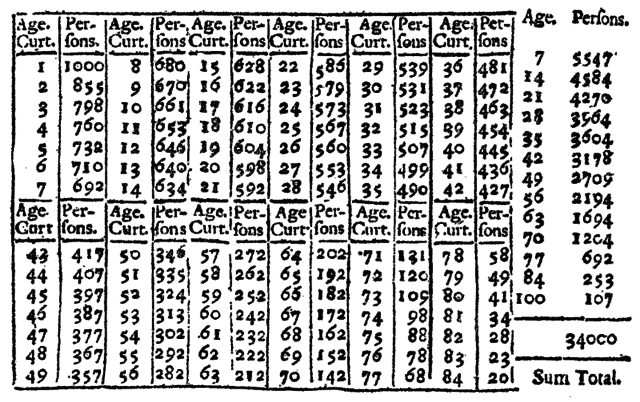
\includegraphics{assets/halley_life_table_1693.png}
\caption{Halley's life table}
\end{figure}

At the outset, Halley's table displayed for each year of age, the number
of people of that age alive in Breslau at the time. Halley estimated
that a total of approximately 34000 people were alive, of which
approximately 1000 were between the ages zero and one, 855 were between
age one and two, and so forth.

Halley saw multiple applications of his table. One of them was to
estimate the proportion of men in a population that could bear arms. To
estimate this proportion he computed the number of people between age 18
and 56, and divided by two. The result suggested that 26\% of the
population were men neither too old nor too young to go to war.

At the same time, King William III of England needed to raise money for
his country's continued involvement in the Nine Years War raging from
1688 to 1697. In 1692, William turned to a financial innovation imported
from Holland, the public sale of life annuities. A life annuity is a
financial product that pays out a predetermined annual amount of money
while the purchaser of the annuity is alive. The king had offered
annuities at fourteen times the annual payout, a price too low for the
young and too high for the old.

Halley recognized that his table could be used to estimate the odds that
a person of a certain age would die within the next year. Based on this
observation, he described a formula for pricing an annuity that,
expressed in modern language, computes the sum of expected discounted
payouts over the course of a person's life starting from their current
age.

\hypertarget{ambitions-of-the-20th-century}{%
\section{Ambitions of the 20th
century}\label{ambitions-of-the-20th-century}}

Halley had stumbled upon the fact that prediction requires no physics.
Unknown outcomes, be they future or unobserved, often follow patterns
found in past observations. This empirical law would become the basis of
consequential decision making for centuries to come.

On the heels of Halley and his contemporaries, the 18th century saw the
steady growth of the life insurance industry. The industrial revolution
fueled other forms of insurance sold to a population seeking safety in
tumultuous times. Corporations and governments developed risk models of
increasing complexity with varying degrees of rigor. Actuarial science
and financial risk assessment became major fields of study built on the
empirical law.

Modern statistics and decision theory emerged in the late 19th and early
20th century. Statisticians recognized that the scope of the empirical
law extended far beyond insurance pricing, that it could be a method for
both scientific discovery and decision making writ large.

Emboldened by advances in probability theory, statisticians modeled
populations as probability distributions. Attention turned to what a
scientist could say about a population by looking at a random draw from
its probability distribution. From this perspective, it made sense to
study how to decide between one of two plausible probability models for
a population in light of available data. The resulting concepts, such as
true positive and false positive, as well as the resulting technical
repertoire, are in broad use today as the basis of hypothesis testing
and binary classification.

As statistics flourished, two other developments around the middle of
the 20th century turned out to be transformational. The works of Turing,
Gödel, and von Neumann, alongside dramatic improvements in hardware,
marked the beginning of the computing revolution. Computer science
emerged as a scientific discipline. General purpose programmable
computers promised a new era of automation with untold possibilities.

World War II spending fueled massive research and development programs
on radar, electronics, and servomechanisms. Established in 1940, the
United States National Defense Research Committee, included a division
devoted to control systems. The division developed a broad range of
control systems, including gun directors, target predictors, and
radar-controlled devices. The agency also funded theoretical work by
mathematician Norbert Wiener, including plans for an ambitious
anti-aircraft missile system that used statistical methods for
predicting the motion of enemy aircraft.

In 1948, Wiener released his influential book \emph{Cybernetics} at the
same time as Shannon released \emph{A Mathematical Theory of
Communication}. Both proposed theories of information and communication,
but their goals were different. Wiener's ambition was to create a new
science, called cybernetics, that unified communications and control in
one conceptual framework. Wiener believed that there was a close analogy
between the human nervous system and digital computers. He argued that
the principles of control, communication, and feedback could be a way
not only to create mind-like machines, but to understand the interaction
of machines and humans. Wiener even went so far as to posit that the
dynamics of entire social systems and civilizations could be understood
and steered through the organizing principles of cybernetics.

The zeitgeist that animated cybernetics also drove ambitions to create
artificial neural networks, capable of carrying out basic cognitive
tasks. Cognitive concepts such as learning and intelligence had entered
research conversations about computing machines and with it came the
quest for machines that learn from experience.

The 1940s were a decade of active research on artificial neural
networks, often called connectionism. A 1943 paper by McCulloch and
Pitts formalized artificial neurons and provided theoretical results
about the universality of artificial neural networks as computing
devices. A 1949 book by Donald Hebb pursued the central idea that neural
networks might learn by constructing internal representations of
concepts.

\hypertarget{pattern-classification}{%
\section{Pattern classification}\label{pattern-classification}}

Around the mid 1950s, it seemed that progress on connectionism had
started to slow and would have perhaps tapered off had psychologist
Frank Rosenblatt not made a striking discovery.

Rosenblatt had devised a machine for image classification. Equipped with
400 photosensors the machine could read an image composed of 20 by 20
pixels and sort it into one of two possible classes. Mathematically, the
Perceptron computes a linear function of its input pixels. If the value
of the linear function applied to the input image is positive, the
Perceptron decides that its input belongs to class 1, otherwise class
-1. What made the Perceptron so successful was the way it could learn
from examples. Whenever it misclassified an image, it would adjust the
coefficients of its linear function via a local correction.

Rosenblatt observed in experiments what would soon be a theorem. If a
sequence of images could at all be perfectly classified by a linear
function, the Perceptron would only make so many mistakes on the
sequence before it correctly classified all images it encountered.

Rosenblatt developed the Perceptron in 1957 and continued to publish on
the topic in the years that followed. The Perceptron project was funded
by the US Office of Naval Research, who jointly announced the project
with Rosenblatt in a press conference in 1958, that led to the New York
Times to exclaim:

\begin{quote}
The Navy revealed the embryo of an electronic computer that it expects
will be able to walk, talk, see, write, reproduce itself and be
conscious of its existence.\footnote{From the New York Times archives:
  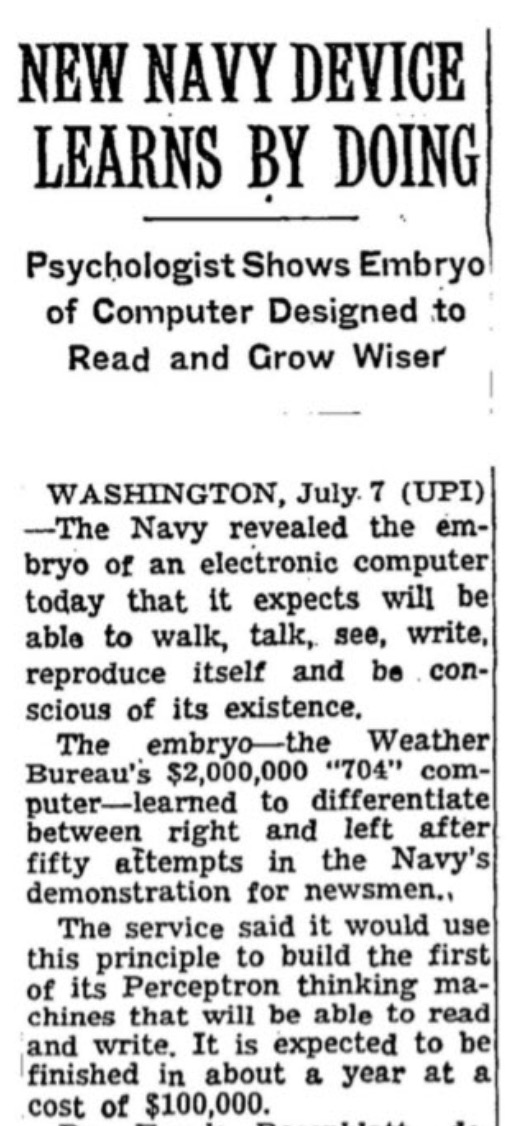
\includegraphics{assets/navy-device.jpg}}
\end{quote}

This development sparked significant interest in perceptrons and
reinvigorated neural networks research throughout the 1960s. By all
accounts, the research in the decade that followed Rosenblatt's work had
essentially all the ingredients of what is now called machine learning,
specifically, supervised learning.

Practitioners experimented with a range of different features and model
architectures, moving from linear functions to Perceptrons with multiple
layers, the equivalent of today's deep neural networks. A range of
variations to the optimization method and different ways of propagating
errors came and went.

Theory followed closely behind. Not long after the invention came a
theorem, called mistake bound, that gave an upper bound on the number of
mistakes the Perceptron would make in the worst case on any sequence of
labeled data points that can be fit perfectly with a linear separator.

Today, we recognize the Perceptron as an instance of the stochastic
gradient method applied to a suitable objective function. The stochastic
gradient method remains the optimization workhorse of modern machine
learning applications.

Shortly after the well-known mistake bound came a lesser known theorem.
The result showed that when the Perceptron succeeded in fitting training
data, it would also succeed in classifying unseen examples correctly
provided that these were drawn from the same distribution as the
training data. We call this \emph{generalization}: Finding rules
consistent with available data that apply to instances we have yet to
encounter.

By the late 1960s, these ideas from perceptrons had solidified into a
broader subject called \emph{pattern recognition} that knew most of the
concepts we consider core to machine learning today. In 1939, Wald
formalized the basic problem of classification as one of optimal
decision making when the data is generated by a known probabilistic
model. Researchers soon realized that pattern classification could be
achieved using data alone to guide prediction methods such as
perceptrons, nearest neighbor classifiers, or density estimators. The
connections with mathematical optimization including gradient descent
and linear programming also took shape during the 1960s.

Pattern classification---today more popularly known as supervised
learning---built on statistical tradition in how it formalized the idea
of generalization. We assume observations come from a fixed data
generating process, such as, samples drawn from a fixed distribution. In
a first optimization step, called training, we fit a model to a set of
data points labeled by class membership. In a second step, called
testing, we judge the model by how well it performs on newly generated
data from the very same process.

This notion of generalization as performance on fresh data can seem
mundane. After all, it simply requires the classifier to do, in a sense,
more of the same. We require consistent success on the same data
generating process as encountered during training. Yet the seemingly
simple question of what theory underwrites the generalization ability of
a model has occupied the machine learning research community for
decades.

\hypertarget{pattern-classification-once-again}{%
\subsection{Pattern classification, once
again}\label{pattern-classification-once-again}}

Machine learning as a field, however, is not a straightforward evolution
of the pattern recognition of the 1960s, at least not culturally and not
historically.

After a decade of perceptrons research, a group of influential
researchers, including McCarthy, Minsky, Newell, and Simon put forward a
research program by the name of artificial intelligence. The goal was to
create human-like intelligence in a machine. Although the goal itself
was in many ways not far from the ambitions of connectionists, the group
around McCarthy fancied entirely different formal techniques. Rejecting
the numerical pattern fitting of the connectionist era, the proponents
of this new discipline saw the future in symbolic and logical
manipulation of knowledge represented in formal languages.

Artificial intelligence became the dominant academic discipline to deal
with cognitive capacities of machines within the computer science
community. Pattern recognition and neural networks research continued,
albeit largely outside artificial intelligence. Indeed, journals on
pattern recognition flourished during the 1970s.

During this time, artificial intelligence research led to a revolution
in \emph{expert systems}, logic and rule based models that had
significant industrial impact. Expert systems were hard coded and left
little room for adapting to new information. AI researchers interested
in such adaptation and improvement---learning, if you will---formed
their own subcommunity, beginning in 1981 with the first International
Workshop on Machine Learning. The early work from this community
reflects the logic-based research that dominated artificial intelligence
at the time; the papers read as if of a different field than what we now
recognize as machine learning research. It was not until the late 1980s
that machine learning began to look more like pattern recognition, once
again.

Personal computers had made their way from research labs into home
offices across wealthy nations. Internet access, if slow, made email a
popular form of communication among researchers. File transfer over the
internet allowed researchers to share code and datasets more easily.

Machine learning researchers recognized that in order for the discipline
to thrive it needed a way to more rigorously evaluate progress on
concrete tasks. Whereas in the 1950s it had seemed miraculous enough if
training errors decreased over time on any non-trivial task, it was
clear now that machine learning needed better benchmarks.

In the late 1980s, the first widely used benchmarks emerged. Then
graduate student David Aha created the UCI machine learning repository
that made several datasets widely available via FTP. Aiming to better
quantify the performance of AI systems, the Defense Advanced Research
Projects Agency (DARPA) funded a research program on speech recognition
that led to the creation of the influential TIMIT speech recognition
benchmark.

These benchmarks had the data split into two parts, one called training
data, one called testing data. This split elicits the promise that the
learning algorithm must only access the training data when it fits the
model. The testing data is reserved for evaluating the trained model.
The research community can then rank learning algorithms by how well the
trained models perform on the testing data.

Splitting data into training and testing sets was an old practice, but
the idea of reusing such datasets as benchmarks was novel and
transformed machine learning. The \emph{dataset-as-benchmark paradigm}
caught on and became core to applied machine learning research for
decades to come. Indeed, machine learning benchmarks were at the center
of the most recent wave of progress on deep learning. Chief among them
was ImageNet, a large repository of images, labeled by nouns of objects
displayed in the images. A subset of roughly 1 million images belonging
to 1000 different object classes was the basis of the ImageNet Large
Scale Visual Recognition Challenge. Organized from 2010 until 2017, the
competition became a striking showcase for performance of deep learning
methods for image classification.

Increases in computing power and volume of available data were a key
driving factor for progress in the field. But machine learning
benchmarks did more than to provide data. Benchmarks gave researchers a
way to compare results, share ideas, and organize communities. They
implicitly specified a problem description and a minimal interface
contract for code. Benchmarks also became a means of knowledge transfer
between industry and academia.

The most recent wave of machine learning as pattern classification was
so successful, in fact, that it became the new artificial intelligence
in the public narrative of popular media. The technology reached
entirely new levels of commercial significance with companies competing
fiercely over advances in the space.

This new artificial intelligence had done away with the symbolic
reasoning of the McCarthy era. Instead, the central drivers of progress
were widely regarded as growing datasets, increasing compute resources,
and more benchmarks along with publicly available code to start from.
Are those then the only ingredients needed to secure the sustained
success of machine learning in the real world?

\hypertarget{prediction-and-action}{%
\section{Prediction and action}\label{prediction-and-action}}

Unknown outcomes often follow patterns found in past observations. But
what do we do with the patterns we find and the predictions we make?
Like Halley proposing his life table for annuity pricing, predictions
only become useful when they are acted upon. But going from patterns and
predictions to successful actions is a delicate task. How can we even
anticipate the effect of a hypothetical action when our actions now
influence the data we observe and value we accrue in the future?

One way to determine the effect of an action is experimentation: try it
out and see what happens. But there's a lot more we can do if we can
model the situation more carefully. A model of the environment specifies
how an action changes the state of the world, and how in turn this state
results in a gain or loss of utility. We include some aspects of the
environment explicitly as variables in our model. Others we declare
\emph{exogenous} and model as noise in our system.

The solution of how to take such models and turn them into plans of
actions that maximize expected utility is a mathematical achievement of
the 20th century. By and large, such problems can be solved by
\emph{dynamic programming}. Initially formulated by Bellman in 1954,
dynamic programming poses optimization problems where at every time
step, we observe data, take an action, and pay a cost. By chaining these
together in time, elaborate plans can be made that remain optimal under
considerable stochastic uncertainty. These ideas revolutionized
aerospace in the 1960s, and are still deployed in infrastructure
planning, supply chain management, and the landing of SpaceX rockets.
Dynamic programming remains one of the most important algorithmic
building blocks in the computer science toolkit.

Planning actions under uncertainty has also always been core to
artificial intelligence research, though initial proposals for
sequential decision making in AI were more inspired by neuroscience than
operations research. In 1950-era AI, the main motivating concept was one
of \emph{reinforcement learning}, which posited that one should
encourage taking actions that were successful in the past. This
reinforcement strategy led to impressive game-playing algorithms like
Samuel's Checkers Agent circa 1959. Surprisingly, it wasn't until the
1990s that researchers realized that reinforcement learning methods were
approximation schemes for dynamic programming. Powered by this
connection, a mix of researchers from AI and operations research applied
neural nets and function approximation to simplify the approximate
solution of dynamic programming programming problems. The subsequent 30
years have led to impressive advances in reinforcement learning and
approximate dynamic programming techniques culminating in solving the
game of Go and in powering dexterous manipulation in robotic systems.

Central to the reinforcement learning paradigm is understanding how to
balance learning about an environment and acting on it. This balance is
a non-trivial problem even in the case where actions do not lead to a
change in state. In the context of machine learning, experimentation in
the form of taking an action and observing its effect often goes by the
name \emph{exploration}. Exploration reveals the payoff of an action,
but it comes at the expense of not taking an action that we already knew
had a decent payoff. Thus, there is an inherent tradeoff between
exploration and \emph{exploitation} of previous actions. Though in
theory, the optimal balance can be computed by dynamic programming, it
is more common to employ techniques from \emph{bandit optimization} that
are simple and effective strategies to balance exploration and
exploitation.

Not limited to experimentation, causality is a comprehensive conceptual
framework to reason about the effect of actions. Causal inference, in
principle, allows us to estimate the effect of hypothetical actions from
observational data. A growing technical repertoire of causal inference
is taking various sciences by storm as witnessed in epidemiology,
political science, policy, climate, and development economics.

There are good reasons that many see causality as a promising avenue for
making machine learning methods more robust and reliable. Current
state-of-the-art predictive models remain surprisingly fragile to
changes in the data. Even small natural variations in a data-generating
process can significantly deteriorate performance. There is hope that
tools from causality could lead to machine learning methods that perform
better under changing conditions.

However, causal inference is no panacea. There are no causal insights
without making substantive judgments about the problem that are not
verifiable from data alone. The reliance on hard earned substantive
domain knowledge stands in contrast with the nature of recent advances
in machine learning that largely did without---and that was the point.

\hypertarget{about-this-book}{%
\section{About this book}\label{about-this-book}}

This is a book for all students in the sprawling field of machine
learning. The material we cover supports a one semester graduate
introduction to machine learning. We invite readers from all
backgrounds; some experience with probability, calculus, and linear
algebra suffices.

In its conception, our book is both an old take on something new and a
new take on something old.

Looking at it one way, we return to the roots with our emphasis on
pattern classification. We believe that the practice of machine learning
today is surprisingly similar to pattern classification of the 1960s,
with a few notable innovations from more recent decades.

This is not to understate recent progress. Like many, we are amazed by
the advances that have happened in recent years. Image recognition has
improved dramatically. Even small devices can now reliably recognize
speech. Natural language processing and machine translation have made
massive leaps forward. Machine learning has even been helpful in some
difficult scientific problems, such as protein folding.

However, we think that it would be a mistake not to recognize pattern
classification as a driving force behind these improvements. The
ingenuity behind many advances in machine learning so far lies not in a
fundamental departure from pattern classification, but rather in finding
new ways to make problems amenable to the model fitting techniques of
pattern classification.

Consequently, the first few chapters of this book follow relatively
closely the excellent text ``Pattern Classification and Scene Analysis''
by Duda and Hart, particularly, its first edition from 1973, which
remains relevant today. Indeed, Duda and Hart summarize the state of
pattern classification in 1973, and it bears a striking resemblance to
the core of what we consider today to be machine learning. We add new
developments on representations, optimization, and generalization, all
of which remain topics of evolving, active research.

Looking at it differently, our book departs in some considerable ways
from the way machine learning is commonly taught.

First, our text emphasizes the role that datasets play in machine
learning. A full chapter explores the histories, significance, and
scientific basis of machine learning benchmarks. Although ubiquitous and
taken for granted today, the datasets-as-benchmarks paradigm was a
relatively recent development of the 1980s. Detailed consideration of
datasets, the collection and construction of data, as well as the
training and testing paradigm, tend to be lacking from theoretical
courses on machine learning.

Second, the book includes a modern introduction to causality and the
practice of causal inference that lays to rest dated controversies in
the field. The introduction is self-contained, starts from first
principles, and requires no prior commitment intellectually or
ideologically to the field of causality. Our treatment of causality
includes the conceptual foundations, as well as some of the practical
tools of causal inference increasingly applied in numerous applications.
It's interesting to note that many recent causal estimators reduce the
problem of causal inference in clever ways to pattern classification.
Hence, this material fits quite well with the rest of the book.

Third, our book covers sequential and dynamic models thoroughly. Though
such material could easily fill a semester course on its own, we wanted
to provide the basic elements required to think about making decisions
in dynamic contexts. In particular, given so much recent interest in
reinforcement learning, we hope to provide a self-contained short
introduction to the concepts underpinning this field. Our approach here
follows our approach to supervised learning: we focus on how we would
make decisions given a probabilistic model of our environment, and then
turn to how to take action when the model is unknown. Hence, we begin
with a focus on optimal sequential decision making and dynamic
programming. We describe some of the basic solution approaches to such
problems, and discuss some of the complications that arise as our
measurement quality deteriorates. We then turn to making decisions when
our models are unknown, providing a survey of bandit optimization and
reinforcement learning. Our focus here is to again highlight the power
of prediction. We show that for most problems, pattern recognition can
be seen as a complement to feedback control, and we highlight how
``certainty equivalent'' decision making---where we first use data to
estimate a model and then use feedback control acting as if this model
were true---is optimal or near optimal in a surprising number of
scenarios.

Finally, we attempt to highlight in a few different places throughout
the potential harms, limitations, and social consequences of machine
learning. From its roots in World War II, machine learning has always
been political. Advances in artificial intelligence feed into a global
industrial military complex, and are funded by it. As useful as machine
learning is for some unequivocally positive applications such as
assistive devices, it is also used to great effect for tracking,
surveillance, and warfare. Commercially its most successful use cases to
date are targeted advertising and digital content recommendation, both
of questionable value to society. Several scholars have explained how
the use of machine learning can perpetuate inequity through the ways
that it can put additional burden on already marginalized, oppressed,
and disadvantaged communities. Narratives of artificial intelligence
also shape policy in several high stakes debates about the replacement
of human judgment in favor of statistical models in the criminal justice
system, health care, education, and social services.

There are some notable topics we left out. Some might find that the most
glaring omission is the lack of material on unsupervised learning.
Indeed, there has been a significant amount of work on unsupervised
learning in recent years. Thankfully, some of the most successful
approaches to learning without labels could be described as
\emph{reductions to pattern recognition}. For example, researchers have
found ingenious ways of procuring labels from unlabeled data points, an
approach called self supervision. We believe that the contents of this
book will prepare students interested in these topics well.

In writing this book, our goal was to balance mathematical rigor against
presenting insights we have found useful in the most direct way
possible. In contemporary learning theory important results often have
short sketches, yet making these arguments rigorous and precise may
require dozens of pages of technical calculations. Such proofs are
critical to the community's scientific activities but often make
important insights hard to access for those not yet versed in the
appropriate techniques. On the other hand, many machine learning courses
drop proofs altogether, thereby losing the important foundational ideas
that they contain. We aim to strike a balance, including full details
for as many arguments as possible, but frequently referring readers to
the relevant literature for full details.

\hypertarget{chapter-notes}{%
\section{Chapter notes}\label{chapter-notes}}

Halley's life table has been studied and discussed extensively; for an
entry point, see recent articles by Bellhouse\footnote{Bellhouse, {``A
  New Look at Halley's Life Table,''} \emph{Journal of the Royal
  Statistical Society: Series A (Statistics in Society)} 174, no. 3
  (2011): 823--32.} and Ciecka,\footnote{Ciecka, {``Edmond Halley's Life
  Table and Its Uses,''} \emph{J. Legal Econ.} 15 (2008): 65.} or the
article by Pearson and Pearson.\footnote{Pearson and Pearson, {``The
  History of Statistics in the 17th and 18th Centuries Against the
  Changing Background of Intellectual, Scientific and Religious
  Thought,''} \emph{British Journal for the Philosophy of Science} 32,
  no. 2 (1981): 177--83.}

Halley was not the first to create a life table. In fact, what Halley
created is more accurately called a population table. Instead, John
Grount deserves credit for the first life table in 1662 based on
mortality records from London. Considered to be the founder of
demography and an early epidemiologist, Grount's work was in many ways
more detailed than Halley's fleeting engagement with Breslau's
population. However, to Grount's disadvantage the mortality records
released in London at the time did not include the age of the deceased,
thus complicating the work significantly.

Mathematician de Moivre picked up Halley's life table in 1725 and
sharpened the mathematical rigor of Halley's idea. A few years earlier,
de Moivre had published the first textbook on probability theory called
``The Doctrine of Chances: A Method of Calculating the Probability of
Events in Play.'' Although de Moivre lacked the notion of a probability
distribution, his book introduced an expression resembling the normal
distribution as an approximation to the Binomial distribution, what was
in effect the first central limit theorem. The time of Halley coincides
with the emergence of probability. Hacking's book provides much
additional context, particularly relevant are Chapter 12 and
13.\footnote{Hacking, \emph{The Emergence of Probability: A
  Philosophical Study of Early Ideas about Probability, Induction and
  Statistical Inference} (Cambridge University Press, 2006).}

For the history of feedback, control, and computing before cybernetics,
see the excellent text by Mindell.\footnote{Mindell, \emph{Between Human
  and Machine: Feedback, Control, and Computing Before Cybernetics} (JHU
  Press, 2002).} For the cybernetics era itself, see the books by
Kline\footnote{Kline, \emph{The Cybernetics Moment: Or Why We Call Our
  Age the Information Age} (JHU Press, 2015).} and Heims.\footnote{Heims,
  {``The Cybernetics Group,''} 1991.} The prologue from the 1988 edition
of \emph{Perceptrons} by Minsky and Papert presents a helpful historical
perspective. The recent 2017 reprint of the same book contains
additional context and commentary in a foreword by Léon Bottou.

Much of the first International Workshop on Machine Learning was
compiled in an edited volume, which summarizes the motivations and
perspectives that seeded the field.\footnote{Michalski, Carbonell, and
  Mitchell, eds., \emph{Machine Learning: An Artificial Intelligence
  Approach} (Springer-Verlag, 1983).} Langley's article provides helpful
context on the state of evaluation in machine learning in the 1980s and
how the desire for better metrics led to a renewed emphasis on pattern
recognition.\footnote{Langley, {``The Changing Science of Machine
  Learning''} (Springer, 2011).} Similar calls for better evaluation
motivated the speech transcription program at DARPA, leading to the
TIMIT data set, arguably the first machine learning benchmark data
set.\footnote{Liberman, {``Obituary: {F}red {J}elinek,''}
  \emph{Computational Linguistics} 36, no. 4 (2010): 595--99; Church,
  {``Emerging Trends: A Tribute to Charles Wayne,''} \emph{Natural
  Language Engineering} 24, no. 1 (2018): 155--60; Liberman and Wayne,
  {``Human Language Technology,''} \emph{{AI} Magazine} 41, no. 2
  (2020): 22--35.}

It is worth noting that the Parallel Distributed Processing Research
Group led by Rummelhart and McLeland actively worked on neural networks
during the 1980s and made extensive use of the rediscovered
back-propagation algorithm, an efficient algorithm for computing partial
derivatives of a circuit.\footnote{McClelland et al., {``Parallel
  Distributed Processing,''} \emph{Explorations in the Microstructure of
  Cognition} 2 (1986): 216--71.}

A recent article by Jordan\footnote{Jordan, {``Artificial
  Intelligence---the Revolution Hasn't Happened Yet,''} \emph{Harvard
  Data Science Review} 1, no. 1 (2019).} provides an insightful
perspective on how the field came about and what challenges it still
faces.

\hypertarget{acknowledgments}{%
\section{Acknowledgments}\label{acknowledgments}}

We are indebted to Alexander Rakhlin, who pointed us to the
generalization result for the Perceptron algorithm by Novikoff. This
result both in its substance and historical position shaped our
understanding of machine learning. Kevin Jamieson was the first to point
out to us the similarity between the structure of our course and the
text by Duda and Hart. Peter Bartlett provided many helpful pointers to
the literature and historical context about generalization theory.
Jordan Ellenberg helped us improve the presentation of algorithmic
stability. Dimitri Bertsekas pointed us to an elegant proof of the
Neyman-Pearson Lemma. We are grateful to Rediet Abebe and Ludwig Schmidt
for discussions relating to the chapter on datasets. We also are
grateful to David Aha, Thomas Dietterich, Michael I. Jordan, Pat
Langley, John Platt, and Csaba Szepesvari for giving us additional
context about the state of machine learning in the 1980s. Finally, we
are indebted to Boaz Barak, David Blei, Adam Klivans, Csaba Szepesvari,
and Chris Wiggins for detailed feedback and suggestions on an early
draft of this text.

We thank all students of UC Berkeley's CS 281a in the Fall of 2019 and
2020, who bore with us as we developed the material of this book.
Special thanks to our graduate student instructors Sarah Dean, Frances
Ding, Sara Fridovich-Keil, Wenshuo Guo, Chloe Hsu, John Miller, Robert
Netzorg, Juan C. Perdomo, and Vickie Ye who spotted and corrected many
mistakes we made.

\chapter{Decision making}

The goal in decision theory is to distinguish between two alternatives
under uncertainty. In this course, we'll focus on modeling uncertainty
with probability and understanding the algorithmic implications of this
view point. The cultural underpinnings of the field choose to start with
an \emph{optimization-based} view of decision theory. Moreover, issues
of which data we collect and how we will represent it will shape our
decision rules. In particular, we will see that when we have full
knowledge of a probabilistic model of the world, the optimal decision
rule will amount to computing a real-valued function of the collected
data, and making decisions based on whether this function is greater
than or less than zero. This sets the stage for the subsequent chapters
on what is now called machine learning: making near-optimal decisions
from data alone, without probabilistic models of the environment.

Our core setup supposes we have two alternative hypotheses~\(H_0\) and
\(H_1\). Given some measured, our goal will be to decide whether~\(H_0\)
or \(H_1\) is true. For example,~\(H_1\) could be the condition under
which a patient has a broken bone and~\(H_0\) the condition of the bone
being unbroken. Or~\(H_1\) could the condition that an email is a spam
message and~\(H_0\) the condition that is not. Under a probabilistic
view of the world,~\(H_0\) and~\(H_1\) each have some \emph{a priori}
probabilities: \[
p_0 = \mathop\mathbb{P}[H_0\,\text{is true}]
\qquad p_1 = \mathop\mathbb{P}[H_1\,\text{is true}]
\] In order to determine which alternative is true, we acquire some data
that hopefully allows us to make an informed prediction. In this book,
we'll always model data as being some random
vector~\(X \in \mathbb{R}^d\) whose distribution varies depending on
whether~\(H_0\) or~\(H_1\) is true. We formalize this by assuming
conditional densities under each hypothesis,
\(p(x \mid H_i\,\text{is true})\) for~\(i=0\) or~\(1\). That is, we
assume a \emph{generative model} also known as a \emph{likelihood
function} under each scenario.\index{likelihood function} Given a model
of priors and likelihood, this chapter will focus on how to make optimal
predictions of the true hypothesis from observed data.

\hypertarget{example-apples-or-oranges}{%
\subsection{Example: Apples or
oranges}\label{example-apples-or-oranges}}

As a simple taxonomy example, consider the case that we are presented
with a piece of fruit, and we know it is either an apple or an orange.
Our observation~\(X\) consists of a set of observable \emph{features} of
the fruit, including perhaps its color, its weight, its sugar content.
If the fruit is an apple, we'd expect its color to range between green
and red. For an orange, we'd expect the colors to vary from orange to
red. From this set of features, our goal will be to decide whether we
have an apple or an orange in front of us.

\hypertarget{example-is-there-a-needle-in-my-haystack}{%
\subsection{Example: Is there a needle in my
haystack?}\label{example-is-there-a-needle-in-my-haystack}}

For a simple example with more mathematical formalism, suppose that when
\(H_0\) is true we observe a scalar~\(X=\omega\) where~\(\omega\) is
unit-variance, zero mean gaussian noise
\(\omega\sim \mathcal{N}(0,1)\).\marginnote{Recall that the gaussian
distribution of mean~\(\mu\) and variance~\(\sigma^2\) is given by the
density
\(\frac{1}{\sigma\sqrt{2\pi}}e^{-\frac12\left(\frac{x-\mu}{\sigma}\right)^2}.\)}
Then suppose when~\(H_1\) is true, we would observe~\(X=s+\omega\) for
some scalar~\(s\). That is, the conditional densities are \[
\begin{aligned}
    p(X\mid H_0\,\text{is true}) &= \mathcal{N}(0,1)\\
    p(X\mid H_1\,\text{is true}) &= \mathcal{N}(s,1)\,.
\end{aligned}
\] When~\(s\) has large magnitude, it would be obvious whether~\(H_0\)
or \(H_1\) were true. For example, suppose~\(s=10\) and we
observed~\(X=11\). Under~\(H_0\), the probability that the observation
greater than~\(10\) is on the order of~\(10^{-23}\), and hence we'd
likely think we're in alternative~\(H_1\). However, if~\(s\) were very
close to zero, distinguishing between the two alternatives is rather
challenging. We can think of a small signal~\(s\) that we're trying to
detect as a \emph{needle in a haystack}.

\begin{figure}
\centering
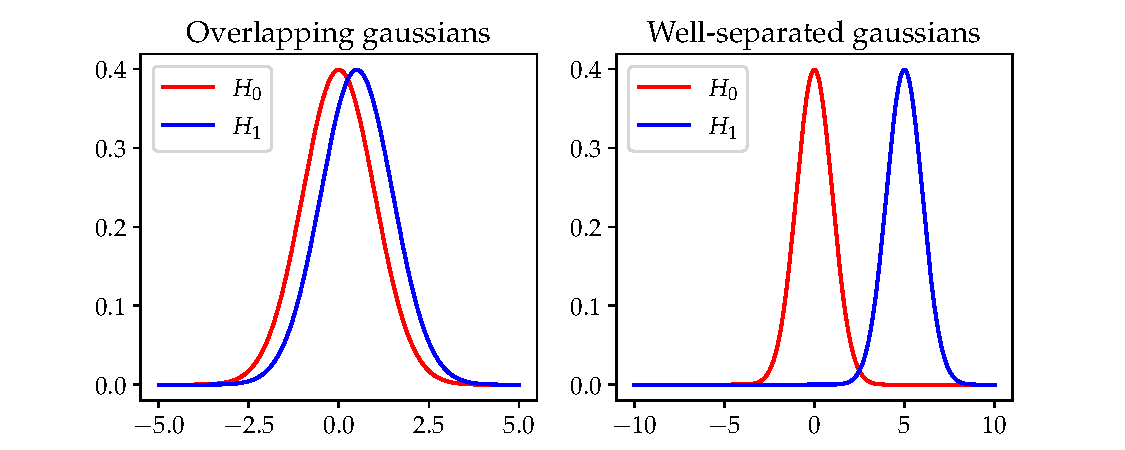
\includegraphics{assets/shifted_gaussians}
\caption{Illustration of shifted gaussians}
\end{figure}

\hypertarget{bayesian-binary-hypothesis-testing}{%
\section{Bayesian binary hypothesis
testing}\label{bayesian-binary-hypothesis-testing}}

Our core approach to all statistical decision making will be to
formulate an appropriate optimization problem for which the decision
rule is the optimal solution. That is, we will optimize over
\emph{algorithms}, searching for functions that map data to decisions
and predictions. We will define an appropriate notion of the cost
associated to each decision, and attempt to construct decision rules
that minimize the expected value of this cost. As we will see, choosing
this optimization framework has many immediate consequences.

\hypertarget{labels}{%
\subsection{Labels}\label{labels}}

In order to neatly write decision problems in the language of
mathematical optimization, we distinguish between boolean and integer
values for the hypotheses. We associate real number valued \emph{labels}
with hypotheses. Labels will be denoted by~\(Y\), and are almost always
integer valued in this book. However, we will describe cases where it is
useful to have vector-valued and real-valued labels when the need
arises. A particularly common example we will use in this chapter is to
set the label~\(Y=1\) when~\(H_1\) is true and~\(Y=0\) when~\(H_0\) is
true. Another common convention is to instead set~\(Y=-1\) when~\(H_0\)
is true. A practitioner is free to choose whatever label mapping is most
convenient for their application.

\hypertarget{loss-functions-and-risk}{%
\subsection{Loss functions and risk}\label{loss-functions-and-risk}}

Define the \emph{loss function} associated with the decision of
declaring \(H_i\) when~\(H_j\) as~\(\ell(i,j)\). This loss could be
symmetric, though often times we want this to be asymmetric. For
instance, we may prefer false positives---where we declare~\(H_1\) is
true even though~\(H_0\) is true---to missed detections----where we
declare~\(H_0\) is true even though~\(H_1\) is
true.\index{loss function}

Suppose we have a function~\(\hat y\) that maps our measurements
in~\(\mathbb{R}^d\) into a discrete integer decision, either~\(0\) to
indicate selection of \(H_0\) or~\(1\) for the selection of~\(H_1\).

\begin{Definition}

We define the \emph{risk} associated with~\(\hat{Y}\) to be \[
    R[f] := \mathop\mathbb{E}[\ell(\hat{Y}(X),Y)]\,.
\] Here, the expectation is taken jointly over~\(X\) and~\(Y.\)

\end{Definition}

Keep in mind that~\(Y=i\) corresponds to the case that~\(H_i\) is true.
Our goal is to determine which decision rule minimizes the
risk.\index{risk}

In order to minimize the risk, we need to solve an \emph{infinite
dimensional} optimization problem over binary-valued functions. That is,
\emph{for every} \(x\), we need to find a binary assignment.
Fortunately, the infinite dimension here turns out to not be a problem
once we make use of the law of iterated expectation. Note \[
\begin{aligned}
    \mathop\mathbb{E}[\ell(\hat{Y}(X),Y)] &= \mathop\mathbb{E}\left[  \mathop\mathbb{E}\left[\ell(\hat{Y}(X),Y)\mid X\right] \right] \\
    &= \int \mathop\mathbb{E}[\ell(\hat{Y}(X),Y)\mid X=x] p(x) \,\mathrm{d} x\,.
\end{aligned}
\] In this last expression, we have a nonnegative combination of terms,
and we have no constraints over the shape of the function~\(f\). Hence,
to minimize, we can treat~\(\hat{Y}(x)\) individually for each fixed
value of \(x\). Indeed, when we fix~\(x\), \[
\begin{aligned}
\mathop\mathbb{E}[\ell(0,Y)\mid X=x]  &= \ell(0,0) \mathop\mathbb{P}[Y=0\mid X=x] + \ell(0,1) \mathop\mathbb{P}[Y=1\mid X=x]\\
\mathop\mathbb{E}[\ell(1,Y)\mid X=x]  &= \ell(1,0) \mathop\mathbb{P}[Y=0\mid X=x] + \ell(1,1) \mathop\mathbb{P}[Y=1\mid X=x]\,.
\end{aligned}
\] And hence, the optimal assignment for this~\(x\) is to pick whichever
of these two expressions is smaller. Collecting terms and rearranging,
we find the decision rule \[
\hat {Y}(x) = \mathbb{1}\left\{\mathop\mathbb{P}[Y=1\mid X=x] \geq  \frac{\ell(1,0)-\ell(0,0)}{\ell(0,1)-\ell(1,1)} \,\, \mathop\mathbb{P}[Y=0\mid X=x]\right\}\,.
\] That is, the optimal rule is to declare~\(H_1\) when the probability
of \(H_1\) given the data~\(x\) is sufficiently larger than the
probability of \(H_0\) given the same data.

Now, we have not explicitly modeled~\(\mathop\mathbb{P}[Y=i\mid X]\),
but we can compute these using Bayes rule: \[
    \mathop\mathbb{P}[Y=i\mid X=x] = \frac{p(x\mid H_i\,\text{is true}) \mathop\mathbb{P}[H_i\,\text{is true}]}{p(x)}\,.
\] Plugging this expression into our decision rule, we find a decision
rule computable only using the probabilities of the hypotheses and our
conditional data observation models \[
\hat {Y}(x) = \mathbb{1}\left\{
    \frac{p(x\mid H_1\,\text{is true})}{p(x\mid H_0\,\text{is true})} \geq  \frac{p_0(\ell(1,0)-\ell(0,0))}{p_1(\ell(0,1)-\ell(1,1))}\right\}\,.
\] This rule is called a \emph{likelihood ratio test} (LRT). The
\emph{likelihood ratio} is simply the ratio of the
likelihoods:\index{likelihood ratio} \[
    \mathcal{L}(x) := \frac{p(x\mid H_1\,\text{is true})}{p(x\mid H_0\,\text{is true})}\,.
\] If we fix \[
\eta =  \frac{p_0(\ell(1,0)-\ell(0,0))}{p_1(\ell(0,1)-\ell(1,1))}\,,
\] then the decision rule that minimizes the risk is \[
    \hat{Y}(x) = \mathbb{1}\{ \mathcal{L}(x)\geq \eta \}\,.
\]

A LRT naturally partitions the sample space in two: \[
\begin{aligned}
\mathcal{X}_0 & = \left\{ x \in \mathcal{X} \colon \mathcal{L}(x) \leq \eta  \right\}\\
\mathcal{X}_1 &=  \left\{ x \in \mathcal{X} \colon \mathcal{L}(x) > \eta  \right\}\,.
\end{aligned}
\] The sample space~\(\mathcal{X}\) then becomes the disjoint union of
\(\mathcal{X}_0\) and~\(\mathcal{X}_1\). Since we only need to identify
which set~\(x\) belongs to, we can use any function
\(h:\mathcal{X} \rightarrow \mathbb{R}\) which gives rise to the same
threshold rule. As long as~\(h(x) \leq t\)
whenever~\(\mathcal{L}(x) \leq \eta\) and vice versa, these functions
give rise to the same partition into \(\mathcal{X}_0\)
and~\(\mathcal{X}_1\). So, for example, if~\(g\) is any monotonically
increasing function, then the decision rule \[
        \hat{Y}_g(x) = \mathbb{1} \{ g(\mathcal{L}(x))\geq g(\eta) \}
\] is equivalent to using~\(\hat{Y}(x)\). In particular, it's popular to
use the logarithmic decision rule \[
    \hat{Y}_{\mathrm{log}}(x)  =  \mathbb{1} \{\log p(x\mid H_1\,\text{is true})- \log p(x\mid H_0\,\text{is true})   \geq \log(\eta)\}\,,
\] as it is often more convenient or mathematically stable to work with
logarithms of likelihoods.

This discussion shows that there are an \emph{infinite number of
functions} which give rise to the same binary decision rule. Hence, we
don't need to know the conditional densities exactly and can still
compute the optimal decision rule. For example, suppose the true
partitioning of the real line under an LRT is \[
  \mathcal{X}_0 = \{x\colon x\geq 0\}\quad\text{and}\quad\mathcal{X}_1 = \{x\colon x< 0\}\,.
\] Setting the threshold to~\(t=0\), the functions~\(h(x) = x\) or
\(h(x)=x^3\) give the same decision rule, as does any odd function which
is positive on the right half line.

\hypertarget{example-needle-in-a-haystack-revisited}{%
\subsection{Example: needle in a haystack
revisited}\label{example-needle-in-a-haystack-revisited}}

Let's return to our needle in a haystack example with
\begin{align*}     p(X\mid H_0\,\text{is true}) &= \mathcal{N}(0,1)\\     p(X\mid H_1\,\text{is true}) &= \mathcal{N}(s,1)\,, \end{align*}
and assume~\(p_1 = 10^{-6}\)---a very rare needle. Suppose that if we
declare~\(H_0\) to be true, we do not pay a cost. If we declare~\(H_1\)
to be true but are wrong, we incur a cost of~\(100\). But if we
guess~\(H_1\) and it is actually true, we actually gain a reward of
\(1,000,000\). That is \[
\ell(0,0) = 0\,,\,\ell(0,1)=0\,,\, \ell(1,0) = 100\,\text{, and}\,\ell(1,1)=-1,000,000\,.
\]

What is the LRT for this problem? Here, it's considerably easier to work
with logarithms: \[
    \log(\eta) = \log\left( \frac{(1-10^{-6}) \cdot 100}{10^{-6} \cdot 10^{6}}\right) \approx 4.61
\] Now, \[
    \log p(x\mid H_1\,\text{is true})- \log p(x\mid H_0\,\text{is true}) =  -\frac{1}{2} (x-s)^2 + \frac{1}{2} x^2 = sx-\frac{1}{2}s^2
\] Hence, the optimal decision rule is to declare~\(H_1\) if
\(sx > \frac{1}{2}s^2+\log(\eta)\) and~\(H_0\) otherwise. The optimal
rule here is \emph{linear}. Moreover, the rule divides the space into
two open intervals. In the case when~\(s\) is positive. \[
    \mathcal{X}_0 = \{ x\colon x\leq  \tfrac{1}{2}s + s^{-1} \log(\eta)\}\,.
\] Also note here that while the entire real line lies in the union of
\(\mathcal{X}_0\) and~\(\mathcal{X}_1\), it is exceptionally unlikely to
ever see an~\(x\) larger than~\(|s|+5\). Hence, even if our decision
rule were incorrect in these regions, the risk would still be nearly
optimal as these terms have almost no bearing on our expected risk!

\hypertarget{canonical-cases-of-likelihood-ratio-tests}{%
\section{Canonical cases of likelihood ratio
tests}\label{canonical-cases-of-likelihood-ratio-tests}}

A folk theorem of statistical decision theory states that essentially
all optimal rules are equivalent to likelihood ratio tests. While this
isn't \emph{always} true, most of the rules used in practice do end up
being equivalent to LRTs. In the next section, we'll present a
mathematical framework that lets us see how far LRTs can take us. But
before that, we can already show that the well known \emph{maximum
likelihood} and \emph{maximum a posteriori} decision rules are both
LRTs.

\hypertarget{maximum-a-posteriori-decision-rule}{%
\subsection{Maximum a posteriori decision
rule}\label{maximum-a-posteriori-decision-rule}}

The expected error of a decision rule is the expected number of times we
declare~\(H_0\) (resp.~\(H_1\)) when~\(H_1\) (resp.~\(H_0\)) is true.
Minimizing the error is equivalent to minimizing the risk with cost
\(\ell(0,0)=\ell(1,1)=0\),~\(\ell(1,0)=\ell(0,1)=1\). The optimum
decision rule is hence a likelihood ratio test. In particular, \[
    \hat{Y}(x) =\mathbb{1}\{ \mathcal{L}(x) \leq \tfrac{p_0}{p_1}\}\,.
\] Using Bayes rule, one can see that this rule is equivalent to \[
    \hat{Y}(x) = \arg \max_i \mathop\mathbb{P}[y=i\mid X=x]\,.
\] The expression~\(\mathop\mathbb{P}[Y\mid X]\) is called the
\emph{posterior probability} of~\(Y\) given~\(X\). And this rule is
hence referred to as the \emph{maximum a posteriori} (MAP) decision
rule.\index{MAP}\index{maximum a posteriori}

\hypertarget{maximum-likelihood-decision-rule}{%
\subsection{Maximum likelihood decision
rule}\label{maximum-likelihood-decision-rule}}

As we discussed above, the expressions~\(p(x\mid H_i)\) are often called
the \emph{likelihood} of the data~\(x\) given the hypothesis~\(H_i\). A
maximum likelihood decision rule would set \[
    \hat{Y}(x) = \arg \max_i p(x\mid H_i)\,.
\] This is completely equivalent to the LRT when~\(p_0=p_1\) and the
costs are~\(\ell(0,0)=\ell(1,1)=0\),~\(\ell(1,0)=\ell(0,1)=1\). Hence,
the maximum likelihood rule is equivalent to the MAP rule with a uniform
prior on the hypothesis.

That both of these popular rules ended up reducing to LRTs is no
accident. In the next lecture, we will show that LRTs are almost always
the optimal solution of optimization-driven decision theory.

\hypertarget{types-of-errors-and-successes}{%
\section{Types of errors and
successes}\label{types-of-errors-and-successes}}

Let~\(\hat{Y}(x)\) denote any decision rule mapping into~\(\{0,1\}\).
Denote \(\mathcal{X}_i = \{x\colon\hat{Y}(x)=i\}\) for~\(i = 0\)
or~\(1\). In this section we define some popular notions of error and
success.

\begin{enumerate}
\def\labelenumi{\arabic{enumi}.}
\tightlist
\item
  \textbf{True Positive Rate:}
  \(\mathrm{TPR} = \mathop\mathbb{P}[\hat{Y}(X)=1\mid H_1\,\text{is true}]\).
  Also known as \emph{power}, \emph{sensitivity}, \emph{probability of
  detection}, or \emph{recall}.
\item
  \textbf{False Negative Rate:} \(\mathrm{FNR} = 1-\mathrm{TPR}\). Also
  known as \emph{type II error} or \emph{probability of missed
  detection}.
\item
  \textbf{False Positive Rate:}
  \(\mathrm{FPR} = \mathop\mathbb{P}[\hat{Y}(X)=1\mid H_0\,\text{is true}]\).
  Also known as \emph{size} or \emph{type I error} or \emph{probability
  of false alarm}.
\item
  \textbf{True Negative Rate} \(\mathrm{TNR}=1-\mathrm{FPR}\), the
  probability of accepting the null hypothesis given the null
  hypothesis. This is also known as
  \emph{specificity}.\index{true positive rate}\index{false positive rate}\index{false negative rate}\index{true negative rate}
\end{enumerate}

There are other quantities that are also of interest in statistics and
machine learning:

\begin{enumerate}
\def\labelenumi{\arabic{enumi}.}
\tightlist
\item
  \textbf{Precision:} \(P[H_1\,\text{is true} \mid \hat{Y}(X)=1]\). This
  is equal to
  \((p_1 \mathrm{TPR})/(p_0 \mathrm{FPR}+p_1 \mathrm{TPR})\).
\item
  \textbf{F1-score:} \(F_1\) is the harmonic mean of precision and
  recall. We can write this as \[
  F_1 = \frac{2 \mathrm{TPR}}{1+\mathrm{TPR}+\tfrac{p_0}{p_1} \mathrm{FPR}}
  \]
\item
  \textbf{False discovery rate:} False discovery rate (FDR) is equal to
  the expected ratio of the number of false positives to the total
  number of positives.
\end{enumerate}

\index{precision}\index{false discovery rate}\index{F1-score}

In the case where both hypotheses are equally likely,
precision,~\(F_1\), and~\(FDR\) are also only functions
of~\(\mathrm{FPR}\) and~\(\mathrm{TPR}\). However, these quantities
explicitly account for \emph{class imbalances}: when there is a
significant skew between~\(p_0\) and~\(p_1\), such measures are often
preferred.

\(\mathrm{TPR}\) and~\(\mathrm{FPR}\) are competing objectives. We'd
like \(\mathrm{TPR}\) as large as possible and~\(\mathrm{FPR}\) as small
as possible. We can write Bayesian decision theory as a problem of
optimizing a balance between~\(\mathrm{TPR}\) and~\(\mathrm{FPR}\): \[
        R[\hat{Y}] := \mathop\mathbb{E}[\ell(\hat{Y}(X),Y)] = \alpha \mathrm{FPR} - \beta \mathrm{TPR} + \gamma\,,
\] where~\(\alpha\) and~\(\beta\) are nonnegative and~\(\gamma\) is some
constant. For all such~\(\alpha\),~\(\beta\), and~\(\gamma\), the
risk-minimizing decision rule is an LRT.

Other cost functions might try to balance~\(\mathrm{TPR}\) versus
\(\mathrm{FPR}\) in other ways. Which of these give rise to LRTs? Each
value of~\(\eta\) in an LRT gives a
pair~\((\mathrm{TPR},\mathrm{FPR})\). The curve traced out in
the~\(\mathrm{TPR}\)-\(\mathrm{FPR}\) plane by varying~\(\eta\) from
negative to positive infinity is called the \emph{receiver operating
characteristic} (ROC) of the likelihood ratio test.\index{ROC}

What pairs of~\((\mathrm{TPR},\mathrm{FPR})\) are achievable using LRTs?
Clearly we can always achieve~\((0,0)\) and~\((1,1)\) with
\(\eta=\pm \infty\). What happens in between these values?

\hypertarget{example-the-needle-one-more-time}{%
\subsection{Example: the needle one more
time}\label{example-the-needle-one-more-time}}

Consider again the example from last lecture where
\(p(x\mid H_0) = \mathcal{N}(0,\sigma^2)\) and
\(p(x\mid H_1) = \mathcal{N}(s,\sigma^2)\) with~\(s\) a positive scalar.
The optimal decision rule is to declare~\(H_1\) when~\(X\) is greater
than \(\gamma:= \frac{s}{2} + \frac{\sigma^2 \log \eta}{s}\). Hence we
have \[
\begin{aligned}
\mathrm{TPR} &= \int_{\gamma}^{\infty} p(x\mid H_1) \,\mathrm{d} x = \tfrac{1}{2} \operatorname{erfc} \left(\frac{\gamma-s}{\sqrt{2}\sigma}\right)\\
\mathrm{FPR} &= \int_{\gamma}^{\infty} p(x\mid H_0) \,\mathrm{d} x = \tfrac{1}{2} \operatorname{erfc} \left(\frac{\gamma}{\sqrt{2}\sigma}\right)\,.
\end{aligned}
\]

For fixed~\(s\) and~\(\sigma\), the ROC curve
\((\mathrm{FPR}(\gamma),\mathrm{TPR}(\gamma))\) only depends on the
\emph{signal to noise ratio} (SNR),~\(s/\sigma\). For small SNR, the ROC
curve is close to the~\(\mathrm{FPR}=\mathrm{TPR}\) line. For large SNR,
\(\mathrm{TPR}\) approaches~\(1\) for all values of~\(\mathrm{FPR}\).

\begin{figure}
\centering
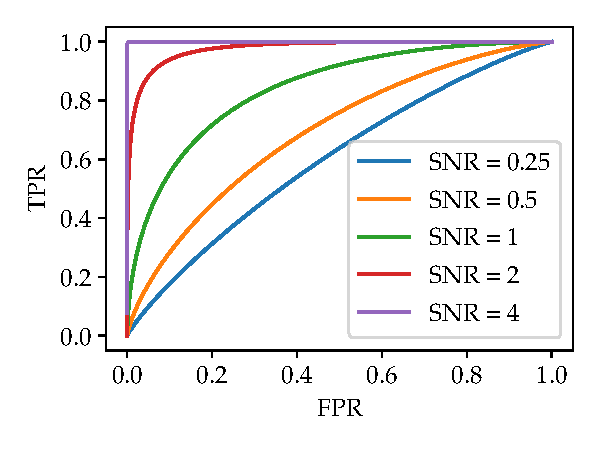
\includegraphics[width=0.75\textwidth,height=\textheight]{assets/gaussian_roc}
\caption{The ROC curves for various signal to noise ratios in the needle
in the haystack problem.}
\end{figure}

\hypertarget{the-neyman-pearson-lemma}{%
\section{The Neyman-Pearson Lemma}\label{the-neyman-pearson-lemma}}

The Neyman-Pearson Lemma, a fundamental lemma of decision theory, will
be an important tool for us to establish three important facts. First,
it will be a useful tool for understanding the geometric properties of
ROC curves. Second, it will demonstrate another important instance where
an optimal decision rule is a likelihood ratio test. Third, it
introduces the notion of probabilistic decision
rules.\index{Neyman-Pearson}

Suppose we want to maximize the probability of detection subject to the
false alarm rate being upper bounded by some fixed number. That is, we
aim to solve the optimization problem: \[
\begin{array}{ll}
    \text{maximize} & \mathrm{TPR}\\
    \text{subject to} & \mathrm{FPR} \leq \alpha
\end{array}
\]

Let's optimize over \emph{probabilistic decision rules}. A probabilistic
decision rule~\(Q\) returns~\(H_1\) with probability~\(Q(x)\)
and~\(H_0\) with probability~\(1-Q(x)\). With such rules, we can rewrite
our optimization problem as: \[
\begin{array}{ll}
    \text{maximize}_Q & \int Q(x) p(x\mid H_1\,\text{is true}) \,\mathrm{d} x\\
    \text{subject to} & \int Q(x) p(x\mid H_0\,\text{is true}) \,\mathrm{d} x \leq \alpha\\
       & \forall x\colon Q(x) \in [0,1]
\end{array}
\]

\begin{Lemma}

\textbf{Neyman-Pearson Lemma.} The optimal probabilistic decision rule
that maximizes~\(\mathrm{TPR}\) with an upper bound on~\(\mathrm{FPR}\)
is a deterministic likelihood ratio test.

\end{Lemma}

Even in this constrained setup, allowing for more powerful probabilistic
rules, we can't escape the inevitability of LRTs. The Neyman-Pearson
Lemma has many interesting consequences in its own right that we will
discuss momentarily. But first, let's see why the lemma is true.

The key insight is that the optimization problem does not depend on the
prior probabilities of~\(H_0\) and~\(H_1\). Hence, we can choose priors
and a loss function to construct a Bayesian Hypothesis testing problem
for which an LRT is optimal. The optimality condition for this chosen
problem will imply the lemma.

\begin{Proof}

Let~\(\eta\) be the threshold for an LRT such that the decision rule \[
 Q_\eta(x)= \mathbb{1}\{ \mathcal{L}(x) > \eta\}
\] has FPR=\(\alpha\). Let~\(\beta\) denote the TPR of~\(Q_\eta\). Note
that \(Q_\eta\) is optimal for the risk minimization problem where we
minimize the probability of error, keep the likelihood functions the
same, but adjust the priors to be \[
    \hat{p}_0=\frac{\eta}{1+\eta} \qquad\qquad\qquad \hat{p}_1 = \frac{1}{1+\eta}\,.
\] That is,~\(Q_\eta\) is the MAP rule for this choice of~\(\hat{p}_0\)
and \(\hat{p}_1\). Now let~\(Q\) be any other decision rule with
\(FPR(Q)\leq \alpha\). We have \[
\begin{aligned}
    \hat{p}_0 \alpha + \hat{p}_1 (1-\beta)
    &\leq \hat{p}_0 FPR(Q) + \hat{p}_1 (1-TPR(Q))  \\
    &\leq  \hat{p}_0 \alpha + \hat{p}_1 (1-TPR(Q))\,,
\end{aligned}
\] which implies~\(TPR(Q) \leq \beta\). This in turn means that
\(Q_\lambda\) maximizes~\(TPR\) for all rules with~\(FPR\leq \alpha\),
proving the lemma.

\end{Proof}

\hypertarget{properties-of-roc-curves}{%
\section{Properties of ROC curves}\label{properties-of-roc-curves}}

A specific randomized decision rule that is useful for analysis combines
two other rules. Suppose decision rule one yields
\((\mathrm{FPR}^{(1)},\mathrm{TPR}^{(1)})\) and the second rule achieves
\((\mathrm{FPR}^{(2)},\mathrm{TPR}^{(2)})\). If we flip a biased coin
and use rule one with probability~\(p\) and rule 2 with
probability~\(1-p\), then this yields a randomized decision rule with
\((\mathrm{FPR},\mathrm{TPR}) = (p\mathrm{FPR}^{(1)}+(1-p)\mathrm{FPR}^{(2)} ,p \mathrm{TPR}^{(1)}+(1-p)\mathrm{TPR}^{(2)})\).
Using this rule lets us prove several properties of ROC curves.

\begin{Proposition}

\((0,0)\) and~\((1,1)\) are on the ROC curve.

\end{Proposition}

This proposition follows because~\((0,0)\) is achieved when
\(\eta = \infty\).~\((1,1)\) is achieved when~\(\eta = -\infty\).

\begin{Proposition}

\(\mathrm{TPR} \geq \mathrm{FPR}\).

\end{Proposition}

To see why this proposition is true, fix some~\(\alpha>0\). Using a
randomized rule, we can achieve a decision rule with
\(\mathrm{TPR}=\mathrm{FPR}=\alpha\). But the Neyman-Pearson LRT with
\(\mathrm{FPR}\) constrained to be less than or equal to~\(\alpha\)
achieves a probability of detection greater than or equal to the
randomized rule.

\begin{Proposition}

The ROC curve is concave.

\end{Proposition}

Suppose~\((\mathrm{FPR}(\eta_1),\mathrm{TPR}(\eta_1))\) and
\((\mathrm{FPR}(\eta_2),\mathrm{TPR}(\eta_2))\) are achievable. Then \[
    (t\mathrm{FPR}(\eta_1)+(1-t)\mathrm{FPR}(\eta_2) ,t \mathrm{TPR}(\eta_1)+(1-t)\mathrm{TPR}(\eta_2))
\] is achievable by a randomized test. Fixing
\(\mathrm{FPR} \leq t\mathrm{FPR}(\eta_1)+(1-t)\mathrm{FPR}(\eta_2)\),
we see that the optimal Neyman-Pearson LRT achieves
\(\mathrm{TPR} \geq \mathrm{TPR}(\eta_1)+(1-t)\mathrm{TPR}(\eta_2)\).

\hypertarget{area-under-the-roc-curve}{%
\subsection{Area under the ROC curve}\label{area-under-the-roc-curve}}

A popular summary statistic for evaluating the quality of a decision
function is the area under its associated ROC curve. This is commonly
abbreviated as AUC. In the ROC curve plotted in the previous section, as
the SNR increases, the AUC increases. However, AUC does not tell the
entire story. Here we plot two ROC curves with the same AUC.

\begin{figure}
\centering
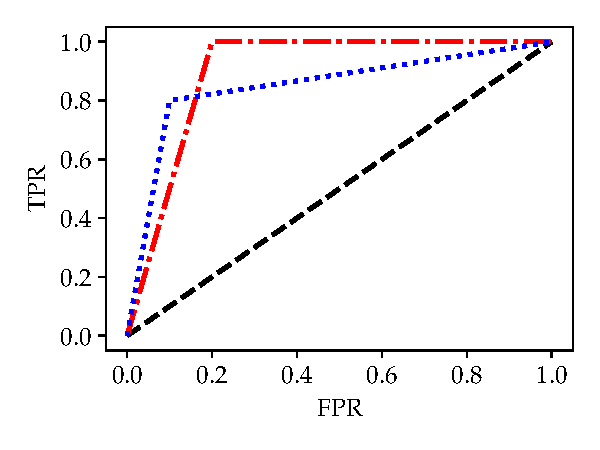
\includegraphics[width=0.75\textwidth,height=\textheight]{assets/equal_auc}
\caption{Two ROC curves with the same AUC. Note that if we constrain
\(\mathrm{FPR}\) to be less than 10\%, for the blue curve,
\(\mathrm{TPR}\) can be as high as 80\% whereas it can only reach 50\%
for the red.}
\end{figure}

If we constrain~\(\mathrm{FPR}\) to be less than 10\%, for the blue
curve, \(\mathrm{TPR}\) can be as high as 80\% whereas it can only reach
50\% for the red. AUC should be always viewed skeptically: the shape of
an ROC curve is always more informative than any individual number.

\hypertarget{looking-ahead-what-if-we-dont-know-the-models}{%
\section{Looking ahead: what if we don't know the
models?}\label{looking-ahead-what-if-we-dont-know-the-models}}

This chapter examined how to make decisions when we have access to known
probabilistic models about both data and priors about the distribution
of hypotheses. The ubiquitous solution to decision problems is a
likelihood ratio test. But note we first derived something even simpler:
a posterior ratio test. That is, we could just compare the probability
of~\(H_1\) given our data to the probability of~\(H_0\) given our data,
and decide on~\(H_1\) if its probability was sufficiently larger than
that of \(H_0\). Comparing likelihoods or posteriors are equivalent up
to a rescaling of the decision threshold.

What if we don't have a probabilistic model of how the data is
generated? There are two natural ways forward: Either estimate
\(p(X\mid H)\) from examples or estimate~\(\mathop\mathbb{P}[Y\mid X]\)
from examples. Estimating likelihood models is a challenge as,
when~\(X\) is high dimensional, estimating~\(p(X\mid H)\) from data is
hard in both theory and practice. Estimating posteriors on the other
hand seems more promising. Estimating posteriors is essentially like
populating an excel spreadsheet and counting places where many columns
are equal to one another.

But estimating the posterior is also likely overkill. We care about the
likelihood or posterior ratios as these completely govern our decision
rules. It's possible that such ratios are easier to estimate than the
quantities themselves. Indeed, we just need to find \emph{any function}
\(f\) where~\(f(x)\geq0\) if
\(p(x\mid H_1\,\text{is true})/p(x\mid H_0\,\text{is true})\geq \eta\)
and \(f(x)\leq0\) if
\(p(x\mid H_1\,\text{is true})/p(x\mid H_0\,\text{is true})\leq \eta\).
So if we only have samples \[
S= \{(x_1,y_1),\ldots (x_n,y_n)\}
\] of data and their labels, we could try to minimize the sample average
\[
    R_S(f) = \frac{1}{n} \sum_{i=1}^n \ell( f(x_i), y_i)
\] with respect to~\(f\). This approach is called \emph{empirical risk
minimization} (ERM) and forms the basis of most contemporary ML and AI
systems. We will devote a the next several chapters of this text to
understanding the ins and outs of ERM.

\hypertarget{decisions-that-discriminate}{%
\section{Decisions that
discriminate}\label{decisions-that-discriminate}}

Binary decision rules always draw a boundary between one group in the
population and its complement. Some are labeled \emph{accept}, others
are labeled \emph{reject}. When decisions have serious consequences for
the individual, however, this decision boundary is not just a technical
artifact. Rather it has moral and legal significance.

Many decisions entail a life changing event for the individual. The
decision could grant access to a major opportunity, such as college
admission, or deny access to a vital resource, such as a social benefit.

The decision maker often has access to data that encode an individual's
status in socially salient groups relating to race, ethnicity, gender,
religion, or disability status. These and other categories that have
been used as the basis of adverse treatment, oppression, and denial of
opportunity in the past and in many cases to this day.

Some see formal or algorithmic decision making as a neutral mathematical
tool. However, numerous scholars have shown how formal models can
perpetuate existing inequities and cause harm. In her book on this
topic, Ruha Benjamin warns of

\begin{quote}
the employment of new technologies that reflect and reproduce existing
inequities but that are promoted and perceived as more objective or
progressive than the discriminatory systems of a previous
era.\footnote{Benjamin, \emph{Race After Technology} (Polity, 2019).}
\end{quote}

Even though the problems of inequality and injustice are much broader
than one of formal decisions, we already encounter an important and
challenging facet within the narrow formal setup of this chapter.
Specifically, we are concerned with decision rules that
\emph{discriminate} in the sense of creating an unjustified basis of
differentiation between individuals.\index{discrimination}

A concrete example is helpful. Suppose we want to accept or reject
individuals for a job. Suppose we have a perfect estimate of the number
of hours an individual is going to work in the next 5 years. We decide
that this a reasonable measure of productivity and so we accept every
applicant where this number exceeds a certain threshold. On the face of
it, our rule might seem neutral. However, on closer reflection, we
realize that this decision rule systematically disadvantages individuals
who are more likely than others to make use of their parental leave
employment benefit that our hypothetical company offers. We are faced
with a conundrum. On the one hand, we trust our estimate of
productivity. On the other hand, we consider taking parental leave
\emph{morally irrelevant} to the decision we're making. It should not be
a disadvantage to the applicant. After all that is precisely the reason
why the company is offering a parental leave benefit in the first place.

The simple example shows that statistical accuracy alone is no safeguard
against discriminatory decisions. It also shows that ignoring
\emph{sensitive attributes} is no safeguard either. So what then is
\emph{discrimination} and how can we avoid it? This question has
occupied scholars from numerous disciplines for decades. There is no
simple answer. Before we go into attempts to formalize discrimination in
our statistical decision making setting, it is helpful to take a step
back and reflect on what the law says.

\hypertarget{legal-background-in-the-united-states}{%
\subsection{Legal background in the United
States}\label{legal-background-in-the-united-states}}

The legal frameworks governing decision making differ from country to
country, and from one domain to another. We take a glimpse at the
situation in the United States, bearing in mind that our description is
incomplete and does not transfer to other countries.

Discrimination is not a general concept. It is concerned with socially
salient categories that have served as the basis for unjustified and
systematically adverse treatment in the past. United States law
recognizes certain \emph{protected categories} including race, sex
(which extends to sexual orientation), religion, disability status, and
place of birth.

Further, discrimination is a domain specific concept concerned with
important opportunities that affect people's lives. Regulated domains
include credit (Equal Credit Opportunity Act), education (Civil Rights
Act of 1964; Education Amendments of 1972), employment (Civil Rights Act
of 1964), housing (Fair Housing Act), and \emph{public accommodation}
(Civil Rights Act of 1964). Particularly relevant to machine learning
practitioners is the fact that the scope of these regulations extends to
marketing and advertising within these domains. An ad for a credit card,
for example, allocates access to credit and would therefore fall into
the credit domain.

There are different legal frameworks available to a plaintiff that
brings forward a case of discrimination. One is called \emph{disparate
treatment}, the other is \emph{disparate impact}. Both capture different
forms of discrimination. Disparate treatment is about purposeful
consideration of group membership with the intention of discrimination.
Disparate impact is about unjustified harm, possibly through indirect
mechanisms. Whereas disparate treatment is about \emph{procedural
fairness}, disparate impact is more about \emph{distributive
justice}.\index{disparate impact}\index{disparate treatment}

It's worth noting that anti-discrimination law does not reflect one
overarching moral theory. Pieces of legislation often came in response
to civil rights movements, each hard fought through decades of activism.

Unfortunately, these legal frameworks don't give us a formal definition
that we could directly apply. In fact, there is some well-recognized
tension between the two doctrines.

\hypertarget{formal-non-discrimination-criteria}{%
\subsection{Formal non-discrimination
criteria}\label{formal-non-discrimination-criteria}}

The idea of formal non-discrimination (or \emph{fairness}) criteria goes
back to pioneering work of Anne Cleary and other researchers in the
educational testing community of the 1960s.\footnote{Hutchinson and
  Mitchell, {``50 Years of Test (Un) Fairness: Lessons for Machine
  Learning,''} in \emph{Proceedings of the Conference on Fairness,
  Accountability, and Transparency}, 2019, 49--58.}\index{fairness}

The main idea is to introduce a discrete random variable~\(A\) that
encodes membership status in one or multiple protected classes.
Formally, this random variable lives in the same probability space as
the other covariates~\(X\), the decision~\(\hat Y=\mathbb{1}\{ R > t\}\)
in terms of a score~\(R\), and the outcome~\(Y\). The random
variable~\(A\) might coincide with one of the features in~\(X\) or
correlate strongly with some combination of them.

Broadly speaking, different statistical fairness criteria all equalize
some group-dependent statistical quantity across groups defined by the
different settings of~\(A\). For example, we could ask to equalize
acceptance rates across all groups. This corresponds to imposing the
constraint for all groups~\(a\) and~\(b\):

\[
\mathop\mathbb{P}[\hat Y = 1 \mid A=a] = \mathop\mathbb{P}[\hat Y = 1 \mid A=b]
\]

Researchers have proposed dozens of different criteria, each trying to
capture different intuitions about what is \emph{fair}. Simplifying the
landscape of fairness criteria, we can say that there are essentially
three fundamentally different ones of particular significance:

\begin{itemize}
\tightlist
\item
  Acceptance rate \(\mathop\mathbb{P}[\hat Y = 1]\)
\item
  Error rates \(\mathop\mathbb{P}[\hat Y = 1 \mid Y = 1]\) and
  \(\mathop\mathbb{P}[\hat Y = 1 \mid Y =0]\)
\item
  Outcome frequency given score value
  \(\mathop\mathbb{P}[Y = 1 \mid R = r ]\)
\end{itemize}

The meaning of the first two as a formal matter is clear given what we
already covered. The third criterion needs a bit more motivation. A
useful property of score functions is \emph{calibration} which asserts
that \(\mathop\mathbb{P}[Y = 1\mid R=r]=r\) for all score values~\(r\).
In words, we can interpret a score value~\(r\) as the propensity of
positive outcomes among instances assigned the score value~\(r\). What
the third criterion says is closely related. We ask that the score
values have the same meaning in each group. That is, instances
labeled~\(r\) in one group are equally likely to be positive instances
as those scored~\(r\) in any other group.

The three criteria can be generalized and simplified using three
different conditional independence statements.

\begin{longtable}[]{@{}ccc@{}}
\caption{Non-discrimination criteria}\tabularnewline
\toprule
Independence & Separation & Sufficiency \\
\midrule
\endfirsthead
\toprule
Independence & Separation & Sufficiency \\
\midrule
\endhead
\(R\bot A\) & \(R\bot A \mid Y\) & \(Y\bot A\mid R\) \\
\bottomrule
\end{longtable}

Each of these applies not only to binary prediction, but any set of
random variables where the independence statement holds. It's not hard
to see that independence implies equality of acceptance rates across
groups. Separation implies equality of error rates across groups. And
sufficiency implies that all groups have the same rate of positive
outcomes given a score value.

Researchers have shown that any two of the three criteria are
\emph{mutually exclusive} except in special cases. That means, generally
speaking, imposing one criterion forgoes the other two.

Although these formal criteria are easy to state and arguably natural in
the language of decision theory, their merit as measures of
discrimination has been subject of an ongoing debate.

\hypertarget{merits-and-limitations-of-a-narrow-statistical-perspective}{%
\subsection{Merits and limitations of a narrow statistical
perspective}\label{merits-and-limitations-of-a-narrow-statistical-perspective}}

The tension between these criteria played out in a public debate around
the use of risk scores to predict \emph{recidivism} in pre-trial
detention decisions.

There's a risk score, called COMPAS, used by many jurisdictions in the
United States to assess \emph{risk of recidivism} in pre-trial bail
decisions.\footnote{Recidivism refers to a person's relapse into
  criminal behavior. In the United States, a defendant may either be
  detained or released on a bail prior to the trial in court depending
  on various factors.} Judges may detain defendant in part based on this
score.\index{COMPAS}

Investigative journalists at ProPublica found that Black defendants face
a higher false positive rate, i.e., more Black defendants labeled
\emph{high risk} end up not committing a crime upon release than among
White defendants labeled \emph{high risk}. In other words, the COMPAS
score fails the separation criterion.\index{ProPublica}

A company called Northpointe, which sells the proprietary COMPAS risk
model, pointed out in return that Black and White defendants have equal
recidivism rates \emph{given} a particular score value. That is
defendants, labeled say an 8 for \emph{high risk} would go on to
recidivate at a roughly equal rate in either group. Northpointe claimed
that this property is desirable so that a judge can interpret scores
equally in both groups.

The COMPAS debate illustrates both the merits and limitations of the
narrow framing of discrimination as a classification criterion.

On the hand, the error rate disparity gave ProPublica a tangible and
concrete way to put pressure on Northpointe. The narrow framing of
decision making identifies the decision maker as responsible for their
decisions. As such it can be used to interrogate and possibly intervene
in the practices of an entity.

On the other hand, decisions are always part of a broader system that
embeds structural patterns of discrimination. For example, a measure of
recidivism hinges crucially on existing policing patterns. Crime is only
found where policing activity happens. However, the allocation and
severity of police force itself has racial bias. Some scholars therefore
find an emphasis on statistical criteria rather than structural
determinants of discrimination to be limited.

\hypertarget{chapter-notes-1}{%
\section{Chapter notes}\label{chapter-notes-1}}

This is the unique chapter in the book where the overwhelming consensus
is that the material is settled. Detection theory has not changed much
at all since the 1950s and is essentially considered a ``solved
problem.'' Neyman and Pearson invented the likelihood ratio
test\footnote{Neyman and Pearson, {``On the Use and Interpretation of
  Certain Test Criteria for Purposes of Statistical Inference: Part
  i,''} \emph{Biometrika}, 1928, 175--240.} and later proved their lemma
showing it to be optimal for maximizing true positive rates while
controlling false positive rates.\footnote{Neyman and Pearson, {``On the
  Problem of the Most Efficient Tests of Statistical Hypotheses,''}
  \emph{Philosophical Transactions of the Royal Society of London.
  Series A} 231, no. 694--706 (1933): 289--337.} Wald followed this work
by inventing general Bayes risk minimization in 1939.\footnote{Wald,
  {``Contributions to the Theory of Statistical Estimation and Testing
  Hypotheses,''} \emph{The Annals of Mathematical Statistics} 10, no. 4
  (1939): 299--326.} Wald's ideas were widely adopted during World War
II for the purpose of interpreting RADAR signals which were often very
noisy. Much work was done to improve RADAR operations, and this led to
the formalization that the output of a RADAR system (the receiver)
should be a likelihood ratio, and a decision should be made based on an
LRT. Our proof of Neyman-Pearson's lemma came later, and is due to
Bertsekas and Tsitsiklis (See Section 9.3 of \emph{Introduction to
Probability}\footnote{Bertsekas and Tsitsiklis, \emph{Introduction to
  Probability}, 2nd ed. (Athena Scientific, 2008).}).

Our current theory of detection was fully developed by Peterson,
Birdsall, and Fox in their report on optimal signal
detectability.\footnote{Peterson, Birdsall, and Fox, {``The Theory of
  Signal Detectability,''} \emph{Transactions of the {IRE}} 4, no. 4
  (1954): 171--212.} Peterson, Birdsall, and Fox may have been the first
to propose Receiver Operating Characteristics as the means to
characterize the performance of a detection system, but these ideas were
contemporaneously being applied to better understand psychology and
psychophysics as well.\footnote{Tanner Jr. and Swets, {``A
  Decision-Making Theory of Visual Detection,''} \emph{Psychological
  Review} 61, no. 6 (1954): 401.}

Statistical Signal Detection theory was adopted in the pattern
recognition community at a very early stage. Chow proposed using optimal
detection theory,\footnote{Chow, {``An Optimum Character Recognition
  System Using Decision Functions,''} \emph{{IRE} Transactions on
  Electronic Computers}, no. 4 (1957): 247--54.} and this led to a
proposal by Highleyman to approximate the risk by its sample
average.\footnote{Highleyman, {``Linear Decision Functions, with
  Application to Pattern Recognition,''} \emph{Proceedings of the {IRE}}
  50, no. 6 (1962): 1501--14.} This transition from population risk to
``empirical'' risk gave rise to what we know today as machine learning.

There is a large amount of literature now on the topic of fairness and
machine learning. For a general introduction to the problem and dangers
associated with algorithmic decision making not limited to
discrimination, see the books by Benjamin,\footnote{Benjamin, \emph{Race
  After Technology}.} Broussard,\footnote{Broussard, \emph{Artificial
  Unintelligence: How Computers Misunderstand the World} (MIT Press,
  2018).} Eubanks,\footnote{Eubanks, \emph{Automating Inequality: How
  High-Tech Tools Profile, Police, and Punish the Poor} (St. Martin's
  Press, 2018).} Noble,\footnote{Noble, \emph{Algorithms of Oppression:
  How Search Engines Reinforce Racism} ({NYU} Press, 2018).} and
O'Neil.\footnote{O'Neil, \emph{Weapons of Math Destruction: How Big Data
  Increases Inequality and Threatens Democracy} (Broadway Books, 2016).}
The technical material in our section on discrimination follows Chapter
2 in the text book by Barocas, Hardt, and Narayanan.\footnote{Barocas,
  Hardt, and Narayanan, \emph{Fairness and Machine Learning}
  (fairmlbook.org, 2019).}

\chapter{Supervised learning}

Previously, we talked about decision theory. Our goal was, broadly
speaking, to use available information described by a random variable
\(X\) to make a decision about an unknown outcome~\(Y\).

Decision theory is directly relevant to machine learning. In a
prediction problem,~\(Y\) might be a future outcome and~\(X\) is an
array of available information. In a classification problem, the random
variable \(X\) might describe an instance of an image and~\(Y\) a
categorical description of the image.

In the important special case of a binary outcome~\(Y\), we saw that we
can write an optimal predictor~\(\hat Y\) as a threshold of some scoring
function~\(f\): \[
\hat Y(x) = \mathbb{1}\{f(x) > t\}
\] If our goal is to maximize the true positive rate of our predictor
while constraining its false positive rate, the Neyman-Pearson Lemma
applies. It shows that we can take the score function to be a ratio of
two likelihood functions.

The optimal score function that comes out of the lemma has a serious
limitation in practice, however. To compute the value of the score
function, we need to know a probability density function for the
positive instances in our problem and also one for the negative
instances. But we are often unable to construct or unwilling to assume a
particular density function. As a thought experiment, attempt to imagine
what a probability density function over images labeled \emph{cat} might
look like. Coming up with such a density function appears to be a
formidable task, one that's not intuitively any easier than merely
classifying whether an image contains a cat or not.

In this chapter, we transition from decision theory to learning theory.
What learning theory adds to decision theory is precisely how we can
extract useful score functions from a collection of data points.

\hypertarget{sample-versus-population}{%
\section{Sample versus population}\label{sample-versus-population}}

Let's take a step back to reflect on the interpretation of the pair of
random variables~\((X, Y)\) that we've worked with so far. We think of
the random variables~\((X, Y)\) as modeling a population of instances in
our classification problem. From this pair of random variables, we can
derive other random variables such as a score function~\(f\) and a
predictor~\(\hat Y = \mathbb{1}\{f(X) > t\}\). All of these are random
variables in the same probability space. When we talk about, say, the
true positive rate of the predictor~\(\hat Y\), we therefore make a
statement about the joint distribution of~\((X, Y)\).

In almost all decision making scenarios, however, we do not have access
to the entire population of instances that we will encounter. Neither do
we have a probability model for the joint distribution of the random
variables~\((X, Y)\). The joint distribution is a theoretical construct
that we can reason about, but it doesn't readily tell us what to do when
we don't have precise knowledge of the joint distribution.

What knowledge then do we typically have about the underlying population
and how can we use it algorithmically to find good predictors? In this
chapter we will begin to answer both questions.

First we assume that from past experience we have observed~\(n\) labeled
instances~\((x_1, y_1),...,(x_n, y_n)\). We assume that each data point
\((x_i, y_i)\) is a draw from the same underlying
distribution~\((X, Y)\). Moreover, we will often assume that the data
points are drawn independently. This pair of assumptions is often called
the ``i.i.d. assumption,'' a shorthand for \emph{independent and
identically distributed}.

To give an example, consider a population consisting of all currently
eligible voters in the United States and some of their features, such
as, age, income, state of residence etc. An \emph{i.i.d. sample} from
this population would correspond to a repeated sampling process that
selects a uniformly random voter from the entire reference population.

Sampling is a difficult problem with numerous pitfalls that can strongly
affect the performance of statistical estimators and the validity of
what we learn from data. In the voting example, individuals might be
unreachable or decline to respond. Even defining a good population for
the problem we're trying to solve is often tricky. Populations can
change over time. They may depend on a particular social context,
geography, or may not be neatly characterized by formal criteria. Task
yourself with the idea of taking a random sample of spoken sentences in
the English language, for example, and you will quickly run into these
issues.

In this chapter, as is common in learning theory, we largely ignore
these important issues. We instead focus on the significant challenges
that remain even if we have a well-defined population and an unbiased
sample from it.

\hypertarget{supervised-learning}{%
\section{Supervised learning}\label{supervised-learning}}

\emph{Supervised learning} is the prevalent method for constructing
classifiers from data. The essential idea is very simple. We assume we
have labeled data, in this context also called \emph{training examples},
of the form~\((x_1,y_1), ..., (x_n, y_n),\) where each \emph{example} is
a pair \((x_i,y_i)\) of an \emph{instance} \(x_i\) and a corresponding
\emph{label} \(y_i.\) The word \emph{supervision} refers to the
availability of these labels.

Given such a collection of labeled data points, supervised learning
turns the task of finding a good classifier into an optimization problem
involving these data points. This optimization problem is called
\emph{empirical risk minimization}.

Recall that when we had full knowledge of the joint distribution of
\((X,Y)\), we aimed to minimize the risk of a decision rule. The risk is
equal to the expected value of a \emph{loss function} that measures the
expected discrepancy between the predicted and true labels. For binary
prediction problems, there are four possible pairs of labels
corresponding to true positives, false positives, true negatives, and
false negatives. In this case, the loss function boils down to
specifying a cost to each of the four possibilities. More generally, a
loss function is a function
\(\ell\colon\mathcal{Y}\times\mathcal{Y}\to\mathbb{R}\,.\) The risk was
defined as the expectation \[
R[f] = \mathop\mathbb{E}\left[ \ell (f(X), Y) \right]\,.
\] We will now see its finite sample counterpart.

\begin{Definition}

Given a set of labeled data points~\(S=((x_1,y_1),...,(x_n, y_n))\), the
\emph{empirical risk} of a
classifier~\(f\colon \mathcal{X}\to\mathcal{Y}\) with respect to the
sample~\(S\) is defined as \[
R_S[f] = \frac1n \sum_{i=1}^n \mathbb{\ell}( f(x_i), y_i )\,.
\]

\end{Definition}

\emph{Empirical risk minimization} is the optimization problem of
finding a classifier in a given function family that minimizes the
empirical risk: \[
\min_{f\in\mathcal{F}} R_S[f]
\] Empirical risk serves as a proxy objective for the risk. Whereas the
risk~\(R[f]\) is a population quantity---that is, a property of the
joint distribution~\((X, Y)\) and our classifier~\(f\)---the empirical
risk is a \emph{sample quantity}. Note that when the samples are drawn
i.i.d., the empirical risk is the sample average of the risk, and in
this case by the central limit theorem, we'd expect the sample risk to
closely approximate the risk for a fixed predictor~\(f\). Regardless of
the distribution of~\(S\), however, note that we can always compute the
empirical risk~\(R_S[f]\) entirely from the sample~\(S\) and the
classifier \(f\). Put differently, it's a quantity we can compute from
samples alone.

There is a tautology relating risk and empirical risk that is good to
keep in mind: \[
R[f] = R_S[f] + (R[f] - R_S[f])
\] Although mathematically trivial, the tautology reveals an important
insight. If we somehow find a classifier~\(f\) that achieves small
empirical risk~\(R_S[f]\), we're left worrying about the term
\(R[f]-R_S[f]\), which quantifies how much the empirical risk of~\(f\)
underestimates its risk. We call this difference \emph{generalization
gap} and it is of fundamental importance to machine learning.
Intuitively speaking, it tells us how well the performance of our
classifier transfers from seen examples (the training examples) to
unseen examples (a fresh example from the population) drawn from the
same distribution. This process is called \emph{generalization}.

Generalization is not the only goal of supervised learning. A constant
classifier that always outputs~\(0\) generalizes perfectly well, but is
almost always entirely useless. What we also need is that the classifier
achieves small empirical risk~\(R_S[f]\). Making the empirical risk
small is fundamentally about \emph{optimization}. As a consequence, a
large part of supervised learning deals with optimization. For us to be
able to talk about optimization, we need to commit to a
\emph{representation} of the function class~\(\mathcal{F}\) that appears
in the empirical risk minimization problem. The representation of the
function class, as well as the choice of a suitable loss function,
determines whether or not we can efficiently find an empirical risk
minimizer.

To summarize, introducing empirical risk minimization directly leads to
three important questions that we will work through in turn.

\begin{itemize}
\tightlist
\item
  \textbf{Representation:} What is the class of functions
  \(\mathcal{F}\) we should choose?
\item
  \textbf{Optimization:} How can we efficiently solve the resulting
  optimization problem?
\item
  \textbf{Generalization:} Will the performance of classifier transfer
  gracefully from seen training examples to unseen instances of our
  problem?
\end{itemize}

These three questions are intertwined. Machine learning is not so much
about studying these questions in isolation as it is about the often
delicate interplay between them. Our choice of representation influences
both the difficulty of optimization and our generalization performance.
Improvements in optimization may not help, or could even hurt,
generalization. Moreover, there are aspects of the problem that don't
neatly fall into only one of these categories. The choice of the loss
function, for example, affects all of the three questions above.

There are important differences between the three questions. Results in
optimization, for example, tend to be independent of the statistical
assumptions about the data generating process. We will see a number of
different optimization methods that under certain circumstances find
either a global or local minimum of the empirical risk objective. In
contrast, to reason about generalization, we need some assumptions about
the data generating process. The most common one is the
i.i.d.-assumption we discussed earlier. We will also see several
mathematical frameworks for reasoning about the gap between risk and
empirical risk.

Let's start with a foundational example that illustrates these core
concepts and their interplay.

\hypertarget{a-first-learning-algorithm-the-perceptron}{%
\section{A first learning algorithm: The
perceptron}\label{a-first-learning-algorithm-the-perceptron}}

As we discussed in the introduction, in 1958 the
\href{https://www.nytimes.com/1958/07/08/archives/new-navy-device-learns-by-doing-psychologist-shows-embryo-of.html}{New
York Times} reported the Office of Naval Research claiming the
perceptron algorithm\footnote{Rosenblatt, {``The Perceptron: A
  Probabilistic Model for Information Storage and Organization in the
  Brain,''} \emph{Psychological Review}, 1958, 65--386.} would ``be able
to walk, talk, see, write, reproduce itself and be conscious of its
existence.'' Let's now dive into this algorithm that seemed to have such
unbounded potential.

Toward introducing this algorithm, let's assume we're in a binary
classification problem with labels in~\(\{-1,1\}\) for notational
convenience. The perceptron algorithm aims to find a \emph{linear
separator}\index{linear separator} of the data, that is, a hyperplane
specified by coefficients~\(w\in\mathbb{R}^d\) that so that all positive
examples lie on one side of the hyperplane and all negative ones on the
other.\marginnote{Illustration of a linear separator.
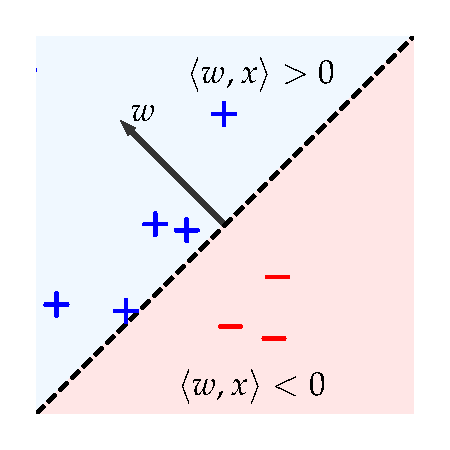
\includegraphics{assets/linear_separator}}

Formally, we can express this as~\(y_i\langle w, x_i\rangle > 0.\) In
other words, the linear function~\(f(x)=\langle w, x\rangle\) agrees in
sign with the labels on all training instances~\((x_i, y_i)\). In fact,
the perceptron algorithm will give us a bit more. Specifically, we
require that the sign agreement has some \emph{margin}
\(y_i\langle w, x_i\rangle \ge 1.\) That is, when~\(y=1,\) the linear
function must take on a value of at least~\(1\) and when~\(y=-1\), the
linear function must be at most~\(-1\). Once we find such a linear
function, our decision rule for new data is
\(\hat{Y}(x) = \mathbb{1}\{ \langle w, x \rangle \geq 0\}\).

The algorithm goes about finding~\(w\) in the following way:

\begin{Algorithm}

\textbf{Perceptron}

\begin{itemize}
\tightlist
\item
  Start from the initial solution \(w_0=0\)
\item
  At each step \(t=0,1,2,...\):

  \begin{itemize}
  \tightlist
  \item
    Select a random index \(i\in\{1,...,n\}\)
  \item
    Case 1: If \(y_i\langle w_t, x_i\rangle < 1\), put \[
    w_{t+1} = w_t + y_i x_i  
    \]
  \item
    Case 2: Otherwise put \(w_{t+1} = w_t\).
  \end{itemize}
\end{itemize}

\end{Algorithm}

Case 1 corresponds to what's called a \emph{margin mistake}. The sign of
the linear function may not disagree with the label, but it doesn't have
the required margin that we asked for.

\begin{figure}
\centering
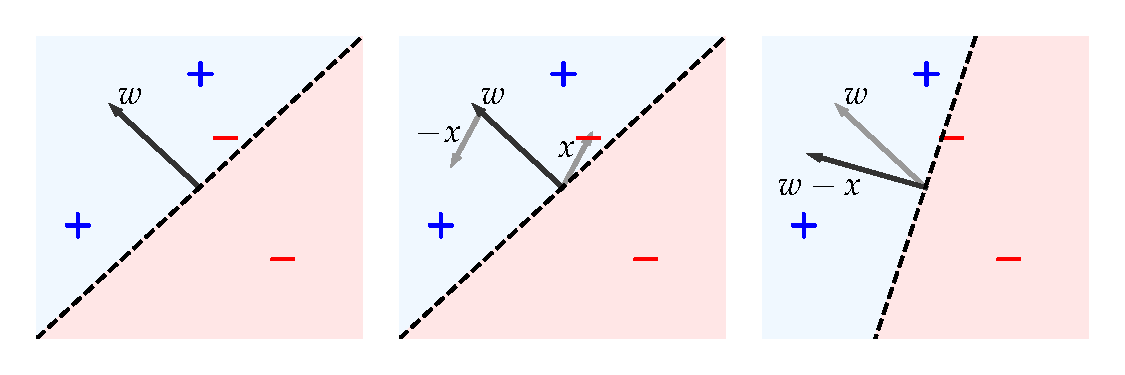
\includegraphics{assets/perceptron}
\caption{Illustration of the perceptron update. Left: One misclassified
example \(x.\) Right: After update.}
\end{figure}

It's common to introduce two \emph{hyperparameters} to the algorithm by
considering the alternative update rule: \[
w_{t+1} = \gamma w_t + \eta y_i x_i
\] Here~\(\eta\) is a positive scalar called a \emph{learning rate} and
\(\gamma\in [0,1]\) is called the \emph{forgetting rate}.

Can we represent the perceptron algorithm as an instance of empirical
risk minimization? The answer is that we can and it is instructive to
see how.

First, it's clear from the description that we're looking for a linear
separator. Hence, our function class is the set of linear functions
\(f(x)=\langle w, x\rangle,\) where~\(w\in\mathbb{R}^d\). We will
sometimes call the vector~\(w\) the \emph{weight vector} or vector of
\emph{model parameters}.

An optimization method that picks a random example at each step and
makes an improvement to the model parameters is the popular stochastic
gradient method specified by the update rule: \[
w_{t+1} = w_t - \eta\nabla_{w_t} \ell(f(x_i), y_i)
\] Here,~\(\nabla \ell(f(x_i), y_i)\) is the gradient of the loss
function with respect to the model parameters~\(w_t\) on a randomly
chosen example \((x_i, y_i)\). We will typically drop the vector~\(w_t\)
from the subscript of the gradient when it's clear from the context. The
scalar~\(\eta>0\) is a step size parameter that we will discuss more
carefully later. For now, think of it as a small constant.

Consider the loss function

\[
\ell(y, \langle w, x\rangle)
= \max(1-y\langle w, x\rangle,\; 0)\,.
\]

\index{loss!hinge}

This loss function is called \emph{hinge loss}.\marginnote{An
illustration of the hinge loss on example \((x, y)\) as a function
of~\(y\langle w, x\rangle\). 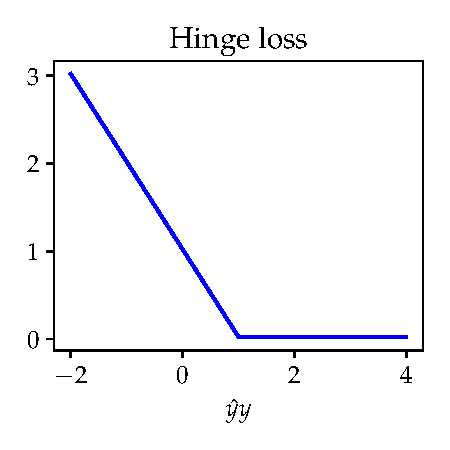
\includegraphics{assets/hinge_loss}} Note
that its gradient is~\(-yx\) when~\(y\langle w, x\rangle < 1\) and~\(0\)
when \(y\langle w, x\rangle >1\).\marginnote{Note that the gradient is
not defined when \(y\langle w, x\rangle=1.\) The loss function is not
differentiable everywhere. This is why technically speaking the
stochastic gradient method operates with what is called a
\emph{subgradient}. The mathematical theory of subgradient optimization
rigorously justifies calling the gradient~\(0\)
when~\(y\langle w, x\rangle=1.\)}

We can see that the hinge loss gives us part of the update rule in the
perceptron algorithm. The other part comes from adding a weight penalty
\(\frac\lambda 2\Vert w\Vert^2\) to the loss function that discourages
the weights from growing out of bounds. This weight penalty is called
\emph{\(\ell_2\)-regularization}, \emph{weight decay}, or \emph{Tikhonov
regularization} depending on which field you work in. The purpose of
regularization is to promote generalization. We will therefore return to
regularization in detail when we discuss generalization in more depth.
For now, note that the margin constraint we introduced is
inconsequential unless we penalize large vectors. Without the weight
penalty we could simply scale up any linear separator until it separates
the points with the desired margin.

Putting the two loss functions together, we get
the~\(\ell_2\)-regularized empirical risk minimization problem for the
hinge loss:

\[
\frac{1}{n}\sum_{i=1}^n \max(1-y_i\langle w, x_i\rangle,\; 0) + \frac\lambda 2 {\Vert w \Vert_2}^2
\]

The perceptron algorithm corresponds to solving this empirical risk
objective with the stochastic gradient method. The constant~\(\eta\),
which we dubbed the learning rate, is the step size of the stochastic
gradient methods. The forgetting rate constant~\(\gamma\) is equal to
\((1-\eta \lambda)\). The optimization problem is also known as
\emph{support vector machine} and we will return to it later on.

\hypertarget{a-word-about-surrogate-losses}{%
\subsection{A word about surrogate
losses}\label{a-word-about-surrogate-losses}}

\index{loss!zero-one}\index{loss!surrogate}

In decision theory, when the goal was to maximize the accuracy of a
predictor, we directly solved the risk minimization with respect to the
\emph{zero-one loss} \[
\ell(y, z)=\mathbb{1}\{y\ne z\}
\] that gives us penalty~\(1\) if our label is incorrect, and
penalty~\(0\) if our predicted label~\(z\) matches the true label~\(y\).
We saw that the optimal classifier in this case was a \emph{maximum a
posteriori} rule, where we selected the label with higher posterior
probability

Why don't we directly solve empirical risk minimization with respect to
the zero-one loss? The reason is that the \emph{empirical} risk with the
zero-one loss is generally difficult to optimize directly. In fact, this
optimization problem is NP-hard even for linear classification
rules.\footnote{It's worth referring back to the derivation of the
  likelihood ratio test to see why similar rules are impossible to
  compute from the empirical risk. In particular, that construction
  relies heavily on iterating conditional expectations, which cannot be
  done from samples.} Take a moment to convince yourself that the
stochastic gradient method, for example, fails entirely on the zero-one
loss objective.

The hinge loss therefore serves a \emph{surrogate loss} for the zero-one
loss. We hope that by optimizing the hinge loss, we end up optimizing
the zero-one loss as well.\marginnote{A comparison of hinge loss versus
zero-one loss. 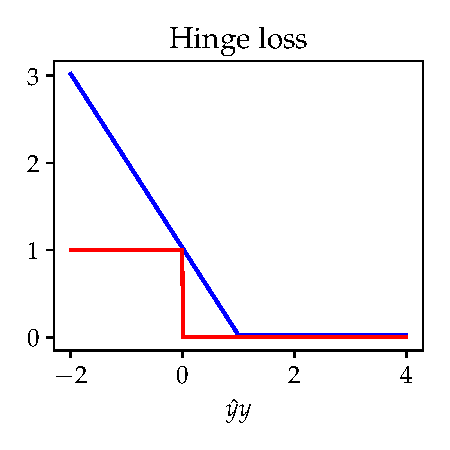
\includegraphics{assets/hinge_vs_zeroone}} The hinge loss
is not the only reasonable choice. There are numerous loss functions
that approximate the zero-one loss in different ways.

\begin{itemize}
\tightlist
\item
  The \emph{hinge loss} is \(\max\{1-yz, 0\}\) and \emph{support vector
  machine} refers to empirical risk minimization with the hinge loss and
  \(\ell_2\)-regularization. This is what the perceptron is optimizing.
\item
  The \emph{squared loss} is given by \(\frac12(y-z)^2\). Linear least
  squares regression corresponds to empirical risk minimization with the
  squared loss. \index{loss!squared}
\item
  The \emph{logistic loss} is \(-\log(\sigma(z))\) when \(y=1\) and
  \(-\log(1-\sigma(z))\) when \(y=-1\), where
  \(\sigma(z) = 1/(1+\exp(-z))\) is the logistic function.
  \emph{Logistic regression} corresponds to empirical risk minimization
  with the logistic loss.
\end{itemize}

Sometimes we can theoretically relate empirical risk minimization under
a surrogate loss to the zero-one loss. In general, however, these loss
functions are used heuristically and performance is evaluated by
trial-and-error.

\hypertarget{formal-guarantees-for-the-perceptron}{%
\subsection{Formal guarantees for the
perceptron}\label{formal-guarantees-for-the-perceptron}}

We saw that the perceptron corresponds to finding a linear classifier
using the stochastic gradient method. What we haven't seen yet is a
proof that the perceptron method works and under what conditions. Recall
that there are two questions we need to address. The first is why the
perceptron method successfully fits the training data, a question about
\emph{optimization}. The second is why the solution should also
correctly classify unseen examples drawn from the same distribution, a
question about \emph{generalization}. We will address each in turn with
results from the 1960s. Even though the analysis here is over 50 years
old, it has all of the essential parts of more recent theoretical
arguments in machine learning.

\hypertarget{mistake-bound}{%
\subsection{Mistake bound}\label{mistake-bound}}

\index{mistake bound}

To see why we perform well on the training data, we use a \emph{mistake
bound} due to Novikoff.\footnote{Novikoff, {``On Convergence Proofs on
  Perceptrons,''} in \emph{Proceedings of the Symposium on the
  Mathematical Theory of Automata}, 1962, 615--22.} The bound shows that
if there exists a linear separator of the training data, then the
perceptron will find it quickly provided that the \emph{margin} of the
separating hyperplane isn't too small.

Margin is a simple way to evaluate how well a classifier separates data.
For a fixed vector~\(w\in \mathbb{R}^d\),~\(w\) defines a hyperplane
\(\mathcal{H}_w = \{x~:~w^Tx=0\}\). Suppose that the hyperplane
\(\mathcal{H}_w\) corresponding to the vector~\(w\) perfectly separates
the data in~\(S\). Then we define the margin of such a vector~\(w\) as
the smallest distance of our data points to this hyperplane: \[
  \gamma(S,w) = \min_{1\le i\le n} \operatorname{dist}(x_i,\mathcal{H}_w )\,.
\] Here, \[
\operatorname{dist}(x, \mathcal{H}_w) = \min\{ \|x - x'\| \colon x'\in \mathcal{H}_w\}
= \frac{|\langle x, w\rangle|}{\|w\|}.
\]

Overloading terminology, we define the margin of a \emph{data set} to be
the maximum margin achievable by any classifier~\(w\): \[
  \gamma(S) = \max_{\Vert w \Vert =1} \gamma(S,w)\,.
\] We will now show that when a data set has a large margin, the
perceptron algorithm will find a separating hyperplane quickly.

Let's consider the simplest form of the perceptron algorithm with
\(\gamma\) and~\(\eta\) both equal to~\(1\). We initialize the algorithm
with \(w_0=0\). The algorithm proceeds by selecting a random
index~\(i_t\) at step~\(t\) checking
whether~\(y_{i_t} w_t^Tx_{i_t} < 1\). If this condition is true, we say
that the algorithm made a \emph{margin mistake}, i.e., the
prediction~\(w_t^T x_{i_t}\) is either wrong or too close to the
hyperplane. If a margin mistake occurs, the perceptron performs the
update \[
    w_{t+1} = w_t + y_{i_t} x_{i_t}\,.
\] That is, we rejigger the hyperplane to be more aligned with the
signed direction of the mistake. If no margin mistake mistakes, then
\(w_{t+1}=w_t\).

We can summarize a worst case analysis of the perceptron algorithm with
the following theorem.

\begin{Theorem}

Define the diameter of the data~\(S\) to be \[
D(S) = \max_{(x,y)\in S}\|x\|\,.
\] The perceptron algorithm makes at most~\((2+D(S)^2)\gamma(S)^{-2}\)
margin mistakes on any sequence of examples~\(S\) that can be perfectly
classified by a linear separator.

\end{Theorem}

\begin{Proof}

The main idea behind the proof of this theorem is that since~\(w\) only
changes when you make a mistake, we can upper bound and lower
bound~\(w\) at each time a mistake is made, and then, by comparing these
two bounds, compute an inequality on the total number of mistakes.

To find an upper bound, suppose that at step~\(t\) the algorithm makes a
margin mistake. We then have the inequality: \[
\begin{aligned}
    \Vert w_{t+1} \Vert^2
    &= \Vert w_t +y_{i_t} x_{i_t}\Vert^2 \\
    & \leq \Vert w_t \Vert^2 + 2 y_{i_t} \langle w_t, x_{i_t}\rangle + \Vert x_{i_t} \Vert^2 \\
    &\leq \Vert w_t\Vert^2 + 2 +  D(S)^2 \,.
\end{aligned}
\] The final inequality uses the fact that
\(y_{i_t} \langle w_t, x_{i_t}\rangle<1\). Now, let~\(m_t\) denote the
total number of mistakes made by the perceptron in the first~\(t\)
iterations. Summing up the above inequality over all the mistakes we
make and using the fact that~\(\|w_0\|=0\), we get our upper bound on
the norm of~\(w_t\): \[
    \Vert w_{t} \Vert \leq \sqrt{m_t(2+ D(S)^2)}\,.
\]

Working toward a lower bound on the norm of~\(w_t,\) we will use the
following argument. Let~\(w\) be any unit vector that correctly
classifies all points in~\(S\). If we make a mistake at iteration~\(t\),
we have \[
  \langle w, w_{t+1}-w_t\rangle
  = \langle w, y_{i_t}x_{i_t}\rangle
  = \frac{|\langle w, x_{i_t}\rangle|}{\|w\|}
  \geq \gamma(S, w)\,.
\] Note that the second equality here holds because~\(w\) correctly
classifies the point~\((x_{i_t}, y_{i_t})\).\marginnote{Convince
yourself that this step fails if~\(w\) does not perfectly separate the
data. This is where we use that the data are linearly separable.} The
inequality follows from the definition of margin.

Now, let~\(w_\star\) denote the hyperplane that achieves the maximum
margin~\(\gamma(S)\). Instantiating the previous argument
with~\(w_\star\), we find that \[
    \Vert w_t \Vert \geq \langle w_\star,  w_t\rangle = \sum_{k=1}^t  w_\star^T (w_{k}-w_{k-1}) \geq m_t\gamma(S)\,,
\] where the equality follows from a telescoping sum
argument.\marginnote{Telescoping sums are a powerful trick used
throughout the analysis of optimization algorithms. The telescoping sum
lets us understand the behavior of the final iterate by decomposing it
into the incremental updates of the individual iterations.}

This yields the desired lower bound on the norm of~\(w_t\). Combined
with the upper bound we already derived, it follows that the total
number of mistakes has the bound \[
m_t \leq \frac{2+D(S)^2}{\gamma(S)^2}\,,
\] as we had hoped to show.

\end{Proof}

The mistake bound does not depend on the dimension of the data. This is
appealing since the requirement of linear separability and high margin,
intuitively speaking, become less taxing the larger the dimension is.

An interesting consequence of this theorem is that if we run the
perceptron repeatedly over the same data set, we will eventually end up
with a separating hyperplane. To see this, imagine repeatedly running
over the data set until no mistake occurred on a full pass over the
data. The mistake bound gives a bound on the number of passes required
before the algorithm terminates.

\hypertarget{from-mistake-bounds-to-generalization}{%
\subsection{From mistake bounds to
generalization}\label{from-mistake-bounds-to-generalization}}

The previous analysis shows that the perceptron finds a good classifier
on the training data. What can we say about new data that we have not
yet seen?

To talk about generalization, we need to make a statistical assumption
about the data generating process. Specifically we assume that the data
points in the training set~\(S=\{(x_1,y_1)\ldots, (x_n,y_n) \}\) where
each drawn i.i.d. from a fixed underlying distribution~\(\mathcal{D}\)
with the labels taking values~\(\{ -1,1 \}\) and
each~\(x_i \in \mathbb{R}^d\).

We know that the perceptron finds a good linear classifier for the
training data (if it exists). What we now show is that this classifier
also works on new data drawn from the same distribution.

To analyze what happens on new data, we will employ a powerful
\emph{stability} argument. Put simply, an algorithm is stable if the
effect of removing or replacing a single data point is small. We will do
a deep dive on stability in our chapter on generalization, but we will
have a first encounter with the idea here.

The Perception is stable because it makes a bounded number of mistakes.
If we remove a data point where no mistake is made, the model doesn't
change at all. In fact, it's as if we had \emph{never seen} the data
point. This lets us relate the performance on seen examples to the
performance on examples in the training data on which the algorithm
never updated.

Vapnik and Chervonenkis presented the following stability argument in
their classic text from 1974, though the original argument is likely a
decade older.\footnote{Vapnik and Chervonenkis, \emph{Theory of Pattern
  Recognition: Statistical Learning Problems} (Moscow: Nauka, 1974).}
Their main idea was to leverage our assumption that the data are i.i.d.,
so we can swap the roles of training and test examples in the analysis.

\begin{Theorem}

Let~\(S_n\) denote a training set of~\(n\) i.i.d. samples from a
distribution~\(\mathcal{D}\) that has a perfect linear separator. Let
\(w(S)\) be the output of the perceptron on a dataset~\(S\) after
running until the hyperplane makes no more margin mistakes on~\(S\).
Let~\(Z=(X,Y)\) be an additional independent sample
from~\(\mathcal{D}\). Then, the probability of making a margin mistake
on~\((X,Y)\) satisfies the upper bound \[
    \mathop\mathbb{P}[Y w(S_n)^T X < 1] \leq \frac{1}{n+1} {\mathop\mathbb{E}}_S\left[ \frac{2+D(S_{n+1})^2}{\gamma(S_{n+1})^2} \right]\,.
\]

\end{Theorem}

\begin{Proof}

First note that \[
\mathop\mathbb{P}[Y w^T X < 1] = \mathop\mathbb{E}[\mathbb{1}\{Yw^T X < 1\}]\,.
\]

Let~\(S_n=(Z_1, ... , Z_n)\) and with~\(Z_k=(X_k, Y_k)\) and put
\(Z_{n+1}=Z=(X,Y)\). Note that these~\(n+1\) random variables are i.i.d.
draws from~\(\mathcal{D}.\) As a purely analytical device, consider the
``leave-one-out set'' \[
S^{-k}=\{Z_1,\dots,Z_{k-1},Z_{k+1},...,Z_{n+1}\}\,.
\] Since the data are drawn i.i.d., running the algorithm on~\(S^{-k}\)
and evaluating it on~\(Z_k=(X_k,Y_k)\) is equivalent to running the
algorithm on~\(S_n\) and evaluating it on~\(Z_{n+1}\). These all
correspond to the same random experiment and differ only in naming.

In particular, we have \[
\mathop\mathbb{P}[Y w(S_n)^T X < 1]
= \frac1{n+1}\sum_{k=1}^{n+1} \mathop\mathbb{E}[\mathbb{1}\{Y_k w(S^{-k})^T X_k < 1\}]\,.
\] Indeed, we're averaging quantities that are each identical to the
left hand side.

But recall from our previous result that the perceptron makes at most \[
m=\frac{2+D((Z_1,\dots,Z_{n+1}))^2}{\gamma((Z_1,\dots,Z_{n+1}))^2}
\] margin mistakes when run on the entire sequence
\((Z_1,\dots,Z_{n+1})\). Let~\(i_1,\dots,i_m\) denote the indices on
which the algorithm makes a mistake in any of its cycles over the data.
If \(k\not\in\{i_1,\dots,i_m\}\), the output of the algorithm remains
the same after we remove the~\(k\)-th sample from the sequence. It
follows that such~\(k\) satisfy~\(Y_k w(S^{-k})X_k \geq 1\) and
therefore~\(k\) does not contribute to the summation above. The other
terms can at most contribute~\(1\) to the summation. Hence, \[
\sum_{k=1}^{n+1}\mathbb{1}\{Y_k w(S^{-k})^T X_k < 1\} \le m\,,
\] and by linearity of expectation, \[
\mathop\mathbb{P}[Y w(S_n)^T X < 1] \le \frac{\mathop\mathbb{E}[m]}{n+1}\,,
\] which is what we wanted to prove.

\end{Proof}

We can turn our mistake bounds into bounds on the empirical risk and
risk achieved by the perceptron algorithm by choosing the loss function
\(\ell(\langle w, x\rangle, y)= \mathbb{1}\{ \langle w, x\rangle y < 1\}\).
These bounds also imply bounds on the (empirical) risk with respect to
the zero-one loss, since the classification error is bounded by the
number of margin mistakes.

\hypertarget{chapter-notes-2}{%
\section{Chapter notes}\label{chapter-notes-2}}

Rosenblatt developed the perceptron in 1957 and continued to publish on
the topic in the years that followed.\footnote{Rosenblatt, \emph{Two
  Theorems of Statistical Separability in the Perceptron} (United States
  Department of Commerce, 1958); Rosenblatt, {``Principles of
  Neurodynamics: Perceptions and the Theory of Brain Mechanisms,''}
  1962.} The perceptron project was funded by the US Office of Naval
Research (ONR), who jointly announced the project with Rosenblatt in a
press conference in 1958, that lead to the New York Times article we
quoted earlier. This development sparked significant interest in
perceptrons research throughout the 1960s.

The simple proof the mistake bound we saw is due to Novikoff.\footnote{Novikoff,
  {``On Convergence Proofs on Perceptrons.''}} Block is credited with a
more complicated contemporaneous proof.\footnote{Block, {``The
  Perceptron: A Model for Brain Functioning,''} \emph{Reviews of Modern
  Physics} 34, no. 1 (1962): 123.} Minsky and Papert attribute a simple
analysis of the convergence guarantees for the perceptron to a 1961
paper by Papert.\footnote{Papert, {``Some Mathematical Models of
  Learning,''} in \emph{London Symposium on Information Theory}
  (Academic Press, New York, 1961).}

Following these developments Vapnik and Chervonenkis proved the
generalization bound for the perceptron method that we saw earlier,
relying on the kind of stability argument that we will return to in our
chapter on generalization. The proof of is available in their 1974
book.\footnote{Vapnik and Chervonenkis, \emph{Theory of Pattern
  Recognition}.} Interestingly, by the 1970s, Vapnik and Chervonenkis
must have abandoned the stability argument in favor of the VC-dimension.

In 1969, Minksy and Papert published their influential book
``perceptrons: an introduction to computational geometry.''\footnote{Minsky
  and Papert, \emph{Perceptrons: An Introduction to Computational
  Geometry} (MIT press, 2017).} Among other results, it showed that
perceptrons fundamentally could not learn certain concepts, like, an XOR
of its input bits. In modern language, linear classifiers cannot learn
parity functions. The results remain relevant in the statistical
learning community and have been extended in numerous ways. On the other
hand, pragmatic researchers realized one could just add the XOR to the
feature vector and continue to use linear methods. We will discuss such
feature engineering in the next chapter.

The dominant narrative in the field has it that Minsky and Papert's book
curbed enthusiasm for perceptron research and their multilayer
extensions, now better known as deep neural networks. In an updated
edition of their book from 1988, Minsky and Papert argue that work on
perceptrons had already slowed significantly by the time their book was
published for a lack of new results:

\begin{quote}
One popular version is that the publication of our book so discouraged
research on learning in network machines that a promising line of
research was interrupted. Our version is that progress had already come
to a virtual halt because of the lack of adequate basic theories,
{[}\ldots{]}.
\end{quote}

On the other hand, the pattern recognition community had realized that
perceptrons were just one way to implement linear decision rules.
Highleyman was arguably the first to propose empirical risk minimization
and applied this technique to optical character recognition.\footnote{Highleyman,
  {``Linear Decision Functions, with Application to Pattern
  Recognition.''}} Active research in the 1960s showed how to find
linear rules using linear programming techniques,\footnote{Mangasarian,
  {``Linear and Nonlinear Separation of Patterns by Linear
  Programming,''} \emph{Operations Research} 13, no. 3 (1965): 444--52.}
and work by Aizerman, Braverman and Rozonoer developed iterative methods
to fit nonlinear rules to data.\footnote{Aizerman, Braverman, and
  Rozonoer, {``The Robbins-Monro Process and the Method of Potential
  Functions,''} \emph{Automation and Remote Control} 26 (1965):
  1882--85.} All of this work was covered in depth in the first edition
of Duda and Hart, which appeared five years after \emph{perceptrons}.

It was at this point that the artificial intelligence community first
split from the pattern recognition community. While the artificial
intelligence community turned towards more \emph{symbolic} techniques in
1970s, work on statistical learning continued in Soviet and IEEE
journals. The modern view of empirical risk minimization, of which we
began this chapter, came out of this work and was codified by Vapnik and
Chervonenkis in the 1970s.

It wasn't until the 1980s that work on pattern recognition, and with it
the tools of the 1960s and earlier, took a stronger foothold in the
machine learning community again.\footnote{Langley, {``The Changing
  Science of Machine Learning.''}} We will continue this discussion in
our chapter on datasets and machine learning benchmarks, which were
pivotal in the return of pattern recognition to the forefront of machine
learning research.

\chapter{Representations and features}

The starting point for prediction is the existence of a vector~\(x\)
from which we can predict the value of~\(y\). In machine learning, each
component of this vector is called a \emph{feature}. We would like to
find a set of features that are good for prediction. Where do features
come from in the first place?

In much of machine learning, the feature vector~\(x\) is considered to
be given. However, features are not handed down from first principles.
They had to be constructed somehow, often based on models that
incorporate assumptions, design choices, and human judgments. The
construction of features often follows human intuition and domain
specific expertise. Nonetheless, there are several principles and
recurring practices we will highlight in this chapter.

Feature representations must balance many demands. First, at a
population level, they must admit decision boundaries with low error
rates. Second, we must be able to optimize the empirical risk
efficiently given then current set of features. Third, the choice of
features also influences the generalization ability of the resulting
model.

There are a few core patterns in feature engineering that are used to
meet this set of requirements. First, there is the process of turning a
measurement into a vector on a computer, which is accomplished by
\emph{quantization and embedding}. Second, in an attempt to focus on the
most discriminative directions, the binned vectors are sorted relative
to their similarity to a set of likely patterns through a process of
\emph{template matching}. Third, as a way to introduce robustness to
noise or reduce and standardize the dimension of data, feature vectors
are compressed into a low, fixed dimension via \emph{histograms and
counts}. Finally, \emph{nonlinear liftings} are used to enable
predictors to approximate complex, nonlinear decision boundaries. These
processes are often iterated, and often times the feature generation
process itself is tuned on the collected data.

\hypertarget{measurement}{%
\section{Measurement}\label{measurement}}

\index{measurement}

Before we go into specific techniques and tricks of trade. It's
important to recognize the problem in full generality. Broadly speaking,
the first step in any machine learning process is to numerically
represent objects in the real world and their relationships in a way
that can be processed by computers.

There is an entire scientific discipline, called measurement theory,
devoted to this subject. The field of measurement theory distinguishes
between a measurement procedure and the target \emph{construct} that we
wish to measure.\footnote{Hand, \emph{Measurement Theory and Practice:
  The World Through Quantification} (Wiley, 2010); Hand,
  \emph{Measurement: A Very Short Introduction} (Oxford University
  Press, 2016); Bandalos, \emph{Measurement Theory and Applications for
  the Social Sciences} (Guilford Publications, 2018).} Physical
temperature, for example, is a construct and a thermometer is a
measurement device. Mathematical ability is another example of a
construct; a math exam can be thought of as a procedure for measuring
this construct.

Practitioners of machine learning should consult with experts on
measurement before creating ad-hoc measurement procedures. More often
than not there is much relevant scholarship on how to measure various
constructs of interest. While we take reliable measurement of certain
physical quantities for granted today, other measurement problems remain
difficult.

Measurement theory has developed a range of sophisticated techniques. In
fact, many measurement procedures themselves involve statistical models
and approximations that blur the line between what is a feature and what
is a model. At the very least, the notion of \emph{raw data} is almost
always an oxymoron.\footnote{Gitelman, \emph{Raw Data Is an Oxymoron}
  (MIT press, 2013).} All data stem from some measurement process that
embeds and operationalizes numerous important choices.

We will return to measurement again when we talk about dataset creation
in Chapter 8.

\hypertarget{human-subjects}{%
\subsection{Human subjects}\label{human-subjects}}

\index{human subjects}

The complexities of measurement are particularly apparent when our
features are about human subjects. Classification problems on human
subjects inevitably involve features that aim quantify a person's
traits, inclinations, abilities, and qualities. We typically try to get
at these constructs by designing surveys, tests, or questionnaires.

Featurization of human subjects can have serious consequences. Recall
the example of using prediction in the context of the criminal justice
system. The figure below shows sample questions that were used to create
the data that the COMPAS recidivism risk score is trained on. These
questions were designed using psychometric models to capture archetypes
of people that might indicate future criminal behavior. Though COMPAS
features have been used to predict recidivism, they have been shown to
be no more predictive than using age, gender, and past criminal
activity.\footnote{Angelino et al., {``Learning Certifiably Optimal Rule
  Lists for Categorical Data,''} \emph{Journal of Machine Learning
  Research} 18, no. 234 (2018): 1--78.}

Machine learning on human subjects should be ethically evaluated in the
same manner as any other scientific investigation with humans. All
interactions must minimize risk to people and must have some possibility
of human benefit. All researchers must not only respect the law but
promote justice. We advise any reader of this book who has not already
done so to take the human subjects training course offered by their
university, where they can learn more about these principles and how to
design measurements that uphold them.

\begin{figure}
\centering
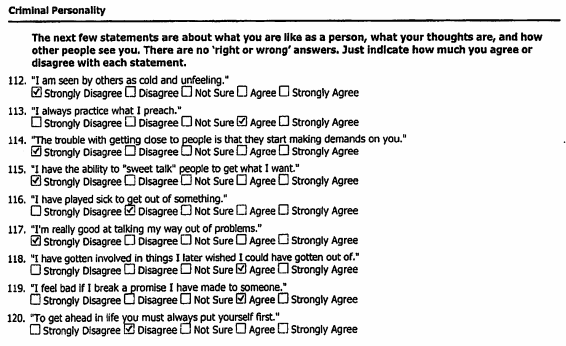
\includegraphics[width=1\textwidth,height=\textheight]{assets/COMPAS.png}
\caption{Sample questions from the COMPAS questionnaire.}
\end{figure}

\hypertarget{quantization}{%
\section{Quantization}\label{quantization}}

\index{quantization}

Signals in the real world are often continuous and we have to choose how
to discretize them for use in a machine learning pipeline. Broadly
speaking, such practices fall under the rubric of \emph{quantization}.
In many cases, our goal is to quantize signals so that we can
reconstruct them almost perfectly. This is the case of high resolution
photography, high fidelity analog-to-digital conversion of audio, or
perfect sequencing of proteins. In other cases, we may want to only
record skeletons of signals that are useful for particular tasks. This
is the case for almost all quantizations of human beings. While we do
not aim to do a thorough coverage of this subject, we note quantization
is an essential preprocessing step in any machine learning pipeline.
Improved quantization schemes may very well translate into improved
machine learning applications. Let us briefly explore a few canonical
examples and issues of quantization in contemporary data science.

\hypertarget{images}{%
\subsection{Images}\label{images}}

Consider the raw bitmap formatting of an image. A bitmap file is an
array indexed by three coordinates. Mathematically, this corresponds to
a \emph{tensor} of order~\(3\). The first two coordinates index space
and the third indexes a color channel. That is,~\(x_{ijk}\) denotes the
intensity at row~\(i\), column~\(j\), and color channel~\(k\). This
representation summarizes an image by dividing two dimensional space
into a regular grid, and then counting the quantity of each of three
primary colors at each grid location.

This pixel representation suffices to render an image on a computer
screen. However, it might not be useful for prediction. Images of the
same scene with different lighting or photographic processes might end
up being quite dissimilar in a pixel representation. Even small
translations of two images might be far apart from each other in a pixel
representation. Moreover, from the vantage point of linear
classification, we could train a linear predictor on any ordering of the
pixels, but scrambling the pixels in an image certainly makes it
unrecognizable. We will describe transformations that address such
shortcomings of pixel representations in the sequel.

\hypertarget{text}{%
\subsection{Text}\label{text}}

Consider a corpus of~\(n\) documents. These documents will typically
have varying length and vocabulary. To embed a document as a vector, we
can create a giant vector for every word in the document where each
component of the vector corresponds to one dictionary word. The
dimension of the vector is therefore the size of the dictionary. For
reach word that occurs in the document we set the corresponding
coordinate of the vector to~\(1\). All other coordinates corresponding
to words not in the document we set to~\(0\).

This is called a \emph{one-hot encoding} of the words in the
dictionary.\index{one-hot encoding} The one-hot encoding might seem both
wasteful due to the high dimension and lossy since we don't encode the
order of the words in the document. Nonetheless, it turns out to be
useful in a number of applications. Since typically the language has
more dictionary words than the length of the document, the encoding maps
a document to a very sparse vector. A corpus of documents would map to a
set of sparse vectors.

\hypertarget{template-matching}{%
\section{Template matching}\label{template-matching}}

\index{template matching}

While quantization can often suffice for prediction problems, we
highlighted above how this might be too fine a representation to encode
when data points are similar or dissimilar. Often times there are higher
level patterns that might be more representative for discriminative
tasks. A popular way to extract these patters is \emph{template
matching}, where we extract the correlation of a feature vector~\(x\)
with a known pattern~\(v\), called \emph{template}.

At a high level, a template match creates a feature~\(x'\) from the
feature~\(x\) by binning the correlation with a template. A simple
example would be to fix a template~\(v\) and compute \[
    x' = \max(v^T x,0)\,.
\] We now describe some more specific examples that are ubiquitous in
pattern classification.

\hypertarget{fourier-cosine-and-wavelet-transforms}{%
\subsection{Fourier, cosine, and wavelet
transforms}\label{fourier-cosine-and-wavelet-transforms}}

One of the foundational patterns that we match to spatial or temporal
data is sinusoids. Consider a vector in~\(\mathbb{R}^d\) and the
transformation with~\(k\)-th component \[
    x_k' = |v_k^T x| \,.
\] Here the~\(\ell\)-th component of~\(v_k\) is given by
\(v_{k\ell} = \exp(2\pi i k \ell/d)\). In this case we are computing the
magnitude of the \emph{Fourier transform} of the feature vector. This
transformation measures the amount of oscillation in a vector. The
magnitude of the Fourier transform has the following powerful property:
Suppose~\(z\) is a translated version of~\(x\) so that \[
    z_k = x_{(k + s) \operatorname{mod} d}
\] for some shift~\(s\). Then one can check that for any~\(v_k\), \[
    |v_k^T x|  = |v_k^T z| \,.
\] That is, the magnitude of the Fourier transform is \emph{translation
invariant}. There are a variety of other transforms that fall into this
category of capturing the transformation invariant content of signals
including cosine and wavelet transforms.

\hypertarget{convolution}{%
\subsection{Convolution}\label{convolution}}

\index{convolution}

For spatial or temporal data, we often consider two data points to be
similar if we can translate one to align with another. For example,
small translations of digits are certainly the same digit. Similarly,
two sound utterances delayed by a few milliseconds are the same for most
applications. \emph{Convolutions} are small templates that are
translated over a feature figure to count the number of occurrences of
some pattern. The output of a convolution will have the same spatial
extent as the input, but will be a ``heat map'' denoting the amount of
correlation with the template at each location in the vector. Multiple
convolutions can be concatenated to add discriminative power. For
example, if one wants to design a system to detect animals in images,
one might design a template for heads, legs, and tails, and then linear
combinations of these appearances might indicate the existence of an
animal.

\hypertarget{summarization-and-histograms}{%
\section{Summarization and
histograms}\label{summarization-and-histograms}}

\index{summarizatio}\index{histogram}

Histograms summarize statistics about counts in data. These serve as a
method for both reducing the dimensionality of an input and removing
noise in the data. For instance, if a feature vector was the temperature
in a location over a year, this could be converted into a histogram of
temperatures which might better discriminate between locations. As
another example, we could downsample an image by making a histogram of
the amount of certain colors in local regions of the image.

\hypertarget{bag-of-words}{%
\subsection{Bag of words}\label{bag-of-words}}

\index{bag of words}

We could summarize a piece of text by summing up the one-hot encoding of
each word that occurs in the text. The resulting vector would have
entries where each component is the number of times the associated word
appears in the document. This is a \emph{bag of words} representation of
the document. A related representation that might take the structure of
text better into account might have a bag of words for every paragraph
or some shorter-length contiguous context.

Bag of words representations are surprisingly powerful. For example,
documents about sports tend to have a different vocabulary than
documents about fashion, and hence are far away from each other in such
an embedding. Since the number of unique words in any given document is
much less than all possible words, bag-of-words representations can be
reasonably compact and sparse. The representations of text as
large-dimensional sparse vectors can be deployed for predicting topics
and sentiment.

\hypertarget{downsamplingpooling}{%
\subsection{Downsampling/pooling}\label{downsamplingpooling}}

Another way to summarize and reduce dimension is to \emph{locally}
average a signal or image. This is called downsampling. For example, we
could break an image into 2x2 grids, and take the average or maximum
value in each grid. This would reduce the image size by a factor of 4,
and would summarize local variability in the image.

\hypertarget{nonlinear-predictors}{%
\section{Nonlinear predictors}\label{nonlinear-predictors}}

Once we have a feature vector~\(x\) that we feel adequately compresses
and summarizes our data, the next step is building a prediction function
\(f(x)\). The simplest such predictors are linear functions of~\(x\),
and linear functions are quite powerful: all of the transformations we
have thus far discussed in this chapter often suffice to arrange data
such that linear decision rules have high accuracy.

However, we oftentimes desire further expressivity brought by more
complex decision rules. We now discuss many techniques that can be used
to build such nonlinear rules. Our emphasis will highlight how most of
these operations can be understood as embedding data in spaces where
linear separation is possible. That is: we seek a nonlinear
transformation of the feature vector so that linear prediction works
well on the transformed features.

\hypertarget{polynomials}{%
\subsection{Polynomials}\label{polynomials}}

\index{polynomials}

Polynomials are simple and natural nonlinear predictors. Consider the
data set in the figure below. Here the data clearly can't be separated
by a linear function, but a quadratic function would suffice. Indeed,
we'd just use the rule that if~\((x_1-c_1)^2+(x_2-c_2)^2 \leq c_3\) then
\((x_1,x_2)\) would have label~\(y=1\). This rule is a quadratic
function of \((x_1,x_2)\).

\begin{figure}
\centering
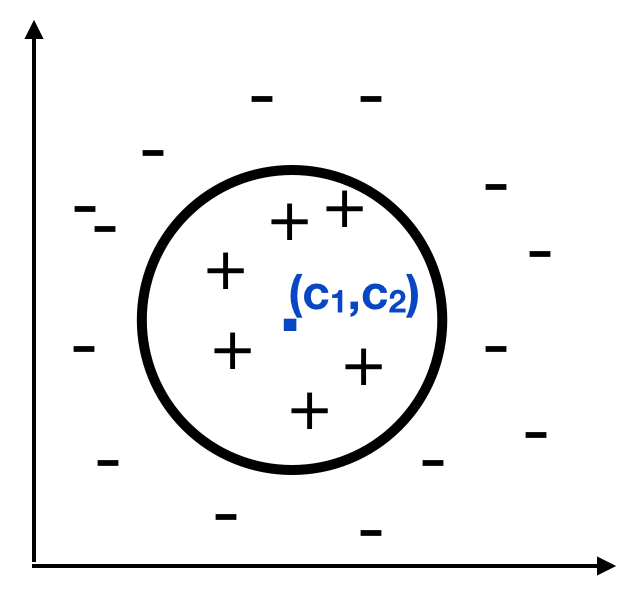
\includegraphics[width=0.5\textwidth,height=\textheight]{assets/poly_classification_cartoon}
\caption{A cartoon classification problem for polynomial classification.
Here, the blue dot denotes the center of the displayed circle.}
\end{figure}

To fit quadratic functions, we only need to fit the \emph{coefficients}
of the function. Every quadratic function can be written as a sum of
quadratic monomials. This means that we can write quadratic function
estimation as fitting a \emph{linear} function to the feature vector: \[
\Phi_2^{\text{poly}}(x) =   \begin{bmatrix} 1& x_1 &x_2 & x_1^2 & x_1 x_2 & x_2^2
    \end{bmatrix}^T
\] Any quadratic function can be written as
\(w^T \Phi_2^{\text{poly}}(x)\) for some~\(w\). The map
\(\Phi_2^{\text{poly}}\) is a \emph{lifting function} that transforms a
set of features into a more expressive set of features.

The features associated with the quadratic polynomial lifting function
have an intuitive interpretation as crossproducts of existing features.
The resulting prediction function is a linear combination of pairwise
products of features. Hence, these features capture co-occurrence and
correlation of a set of features.

The number of coefficients of a generic quadratic function in~\(d\)
dimensions is \[
{{d+2} \choose 2}\,,
\] which grows quadratically with dimension. For general degree~\(p\)
polynomials, we could construct a lifting function
\(\Phi_p^{\text{poly}}(x)\) by listing all of the monomials with degree
at most~\(p\). Again, any polynomial of degree~\(p\) can be written as
\(w^T \Phi_p^{\text{poly}}(x)\) for some~\(w\). In this case,
\(\Phi_p^{\text{poly}}(x)\) would have \[
{{d+p} \choose p}
\] terms, growing roughly as~\(d^p\). It shouldn't be too surprising to
see that as the degree of the polynomial grows, increasingly complex
behavior can be approximated.

\hypertarget{how-many-features-do-you-need}{%
\subsection{How many features do you
need?}\label{how-many-features-do-you-need}}

Our discussion of polynomials led with the motivation of creating
nonlinear decision boundaries. But we saw that we could also view
polynomial boundaries as taking an existing feature set and performing a
nonlinear transformation to embed that set in a higher dimensional space
where we could then search for a linear decision boundary. This is why
we refer to nonlinear feature maps as \emph{lifts}.

Given expressive enough functions, we can always find a lift such that a
particular data set can be mapped to any desired set of labels. How high
of a dimension is necessary? To gain insights into this question, let us
stack all of the data points~\(x_1,\ldots,x_n \in\mathbb{R}^d\) into a
matrix~\(X\) with~\(n\) rows and~\(d\) columns. The predictions across
the entire data set can now be written as \[
 \hat{y} = Xw\,.
\] If the~\(x_i\) are linearly independent, then as long
as~\(d \geq n\), we can make \emph{any} vector of predictions~\(y\) by
finding a corresponding vector~\(w\). For the sake of
\emph{expressivity}, the goal in feature design will be to find lifts
into high dimensional space such that our data matrix~\(X\) has linearly
independent columns. This is one reason why machine learning
practitioners lean towards models with more parameters than data points.
Models with more parameters than data points are called
\emph{overparameterized}.

\index{overparameterized}

As we saw in the analysis of the perceptron, the key quantities that
governed the number of mistakes in the perceptron algorithm were the
maximum norm of~\(x_k\) and the norm of the optimal~\(w\). Importantly,
the dimension of the data played no role. Designing features where~\(w\)
has controlled norm is a domain specific challenge, but has nothing to
do with dimension. As we will see in the remainder of this book, high
dimensional models have many advantages and few disadvantages in the
context of prediction problems.

\hypertarget{basis-functions}{%
\subsection{Basis functions}\label{basis-functions}}

\index{basis functions}

Polynomials are an example of \emph{basis functions}. More generally, we
can write prediction functions as linear combinations of~\(B\) general
nonlinear functions~\(\{b_k\}\): \[
    f(x) = \sum_{k=1}^{B} w_k b_k(x)
\] In this case, there is again a lifting function
\(\Phi_{\text{basis}}(x)\) into~\(B\) dimensions where the~\(k\)th
component is equal to~\(b_k(x)\)
and~\(f(x) =w^T \Phi_{\text{basis}}(x)\). There are a variety of basis
functions used in numerical analysis including trigonometric
polynomials, spherical harmonics, and splines. The basis function most
suitable for a given task is often dictated by prior knowledge in the
particular application domain.

A particularly useful set in pattern classification are the \emph{radial
basis functions}. A radial basis function has the form \[
    b_z(x) = \phi( \Vert x-z \Vert)
\] where~\(z \in \mathbb{R}^d\) and
\(\phi:\mathbb{R}\rightarrow\mathbb{R}\). Most commonly, \[
    \phi(t) = e^{-\gamma t^2}
\] for some~\(\gamma>0\). In this case, given~\(z_1,\ldots, z_k\), our
functions take the form \[
    f_k(x) = \sum_{j=1}^k w_k  e^{-\gamma \Vert x-z_k \Vert^2}\,.
\] Around each anchor point~\(z_k\), we place a small Gaussian bump.
Combining these bumps with different weights allows us to construct
arbitrary functions.

\begin{figure}
\centering
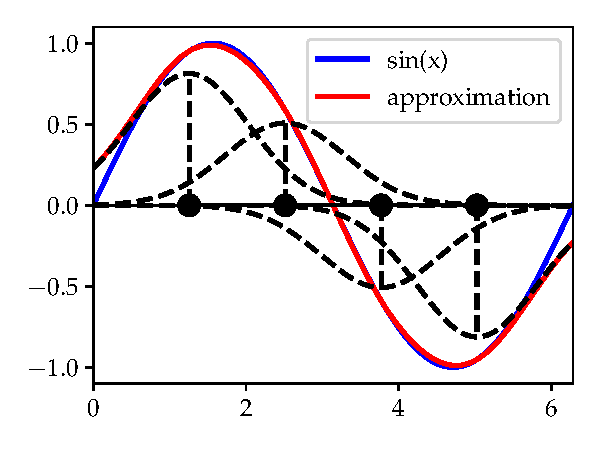
\includegraphics[width=0.75\textwidth,height=\textheight]{assets/rbf_approximation}
\caption{Radial Basis Function approximation of sin(x). We plot the four
Gaussian bumps that sum to approximate the function.}
\end{figure}

How to choose the~\(z_k\)? In low dimensions,~\(z_k\) could be placed on
a regular grid. But the number of bases would then need to scale
exponentially with dimension. In higher dimensions, there are several
other possibilities. One is to use the set of training data. This is
well motivated by the theory of \emph{reproducing kernels}. Another
option would be to pick the~\(z_k\) at random, inducing \emph{random
features}. A third idea would be to search for the best~\(z_i\). This
motivates our study of \emph{neural networks}. As we will now see, all
three of these methods are powerful enough to approximate any desired
function, and they are intimately related to each other.

\hypertarget{kernels}{%
\subsection{Kernels}\label{kernels}}

\index{kernel}

One way around high dimensionality is to constrain the space of
prediction function to lie in a low dimensional subspace. Which subspace
would be useful? In the case of linear functions, there is a natural
choice: the span of the training data. By the fundamental theorem of
linear algebra, any vector in~\(\mathbb{R}^d\) can be written as sum of
a vector in the span of the training data and a vector orthogonal to all
of the training data. That is, \[
    w = \sum_{i=1}^n \alpha_i x_i + v
\] where~\(v\) is orthogonal to the~\(x_i\). But if~\(v\) is orthogonal
to every training data point, then in terms of prediction, \[
    w^T x_i = \sum_{j=1}^n \alpha_j x_j^T x_i \,.
\] That is, the~\(v\) has no bearing on in-sample prediction whatsoever.
Also note that prediction is only a function of the dot products between
the training data points. In this section, we consider a family of
prediction functions built with such observations in mind: we will look
at functions that expressly let us compute dot products between liftings
of points, noting that our predictions will be linear combinations of
such lifted dot products.

Let~\(\Phi(x)\) denote any lifting function. Then \[
    k(x,z) := \Phi(x)^T \Phi(z)
\] is called the \emph{kernel function} associated with the feature map
\(\Phi\). Such kernel functions have the property hat for for any
\(x_1,\ldots, x_n\), the matrix K with entries \[
    K_{ij} = k(x_i,x_j)
\] is positive semidefinite. This turns out to be the key property to
define kernel functions. We say a symmetric function
\(k:\mathbb{R}^d \times \mathbb{R}^d \rightarrow \mathbb{R}\) is a
kernel function if it has this positive semidefiniteness property.

It is clear that positive combinations of kernel functions are kernel
functions, since this is also true for positive semidefinite matrices.
It is also true that if~\(k_1\) and~\(k_2\) are kernel functions, then
so is \(k_1 k_2\). This follows because the elementwise product of two
positive semidefinite matrices is positive semidefinite.

Using these rules, we see that the function \[
    k(x,z) = (a +b x^Tz)^p
\] where~\(a,b\geq 0\),~\(p\) a positive integer is a kernel function.
Such kernels are called a polynomial kernels. For every polynomial
kernel, there exists an associated lifting function~\(\Phi\) with each
coordinate of~\(\Phi\) being a monomial such that \[
    k(x,z) =\Phi(x)^T \Phi(z) \,.
\]

As a simple example, consider the 1-dimensional case of a kernel \[
    k(u,v) = (1+uv)^2\,.
\] Then~\(k(u,v) =\Phi(u)^T \Phi(v)\) for \[
\Phi(u) = \begin{bmatrix} 1\\ \sqrt{2} u \\ u^2
\end{bmatrix}\,.
\]

We can generalize polynomial kernels to \emph{Taylor Series} kernels.
Suppose that the one dimensional function~\(h\) has a convergent Taylor
series for all~\(t \in [-R,R]\): \[
    h(t) = \sum_{j=1}^\infty a_j t^j
\] where~\(a_j \geq 0\) for all~\(j\). Then the function \[
    k(x,z) = h(\langle x, z \rangle)
\] is a positive definite kernel. This follows because each term
\(<x,z>^j\) is a kernel, and we are taking a nonnegative combination of
these polynomial kernels. The feature space of this kernel is the span
of the monomials of degrees where the~\(a_j\) are nonzero.

Two example kernels of this form are the \emph{exponential kernel} \[
    k(x,z) = \exp(-\gamma \langle x, z\rangle)
\] and the \emph{arcsine kernel} \[
    k(x,z) = \sin^{-1}(\langle x,z \rangle)\,,
\] which is a kernel for~\(x\),~\(z\) on the unit sphere.

Another important kernel is the Gaussian kernel: \[
    k(x,z) = \exp(-\tfrac{\gamma}{2} \Vert x-z\Vert^2)\,.
\] The Gaussian kernel can be thought of as first lifting data using the
exponential kernel then projecting onto the unit sphere in the lifted
space.

We note that there are many kernels with the same feature space. Any
Taylor Series kernel with positive coefficients will have the same set
of features. The feature space associated Gaussian kernel is equivalent
to the span of radial basis functions. What distinguishes the kernels
beyond the features they represent? The key is to look at the norm.
Suppose we want to find a fit of the form \[
    f(x_j) = w^T \Phi(x_j)\qquad \text{for}~j=1,2,\ldots,n\,.
\] In the case when~\(\Phi\) maps into a space with more dimensions than
the number of data points we have acquired, there will be an infinite
number of~\(w\) vectors that perfectly interpolate the data. As we saw
in our introduction to supervised learning, a convenient means to pick
an interpolator is to choose the one with smallest norm. Let's see how
the norm interacts with the form of the kernel. Suppose our kernel is a
Taylor series kernel \[
    h(t) = \sum_{j=1}^\infty a_j \langle x, z \rangle^j\,.
\] Then the smaller~\(a_j\), the larger the corresponding~\(w_j\) should
have to be. Thus, the~\(a_j\) in the kernel expansion govern how readily
we allow each feature in a least-norm fit. If we consider the
exponential kernel with parameter~\(\gamma\),
then~\(a_j = \gamma^j/j!\). Hence, for large values of~\(\gamma\), only
low degree terms will be selected. As we decrease~\(\gamma\), we allow
for higher degree terms to enter the approximation. Higher degree terms
tend to be more sensitive to perturbations in the data than lower degree
ones, so~\(\gamma\) should be set as large as possible while still
providing desirable predictive performance.

The main appeal of working with kernel representations is they translate
into simple algorithms with bounded complexity. Since we restrict our
attention to functions in the span of the data, our functions take the
form \[
    f(x) = \left(\sum_{i=1}^n \alpha_i \Phi(x_i)^T \right)\Phi(x) = \sum_{i=1}^n \alpha_i k(x_i,x)\,.
\] We can thus pose all of our optimization problems in terms of the
coefficients~\(\alpha_i\). This means that any particular problem will
have at most~\(n\) parameters to search for. Even the norm of~\(f\) norm
can be computed without explicitly ever computing the feature embedding,
as \[
    \left \Vert\sum_i \alpha_i \Phi(x_i)\right\Vert^2 = \alpha^T K \alpha
\] where~\(K\) is the matrix with~\(ij\)th entry~\(k(x_i,x_j)\). As we
will see in the optimization chapter, such representations turn out to
be optimal in most machine learning problems. Functions learned by ERM
methods on kernel spaces are weighted sums of the similarity (dot
product) between the training data and the new data. When~\(k\) is a
Gaussian kernel, this relationship is even more evident: The optimal
solution is simply a radial basis function whose anchor points are given
by the training data points.

\hypertarget{neural-networks}{%
\subsection{Neural networks}\label{neural-networks}}

\index{neural networks}

Though the name originates from the study of neuroscience, modern neural
nets a have nothing to do with the brain. Neural nets are merely a
composition of differentiable functions, typically alternating between
component wise nonlinearities and linear maps. The simplest example of a
neural network would be \[
    f(x) = w^T \sigma(Ax+b)
\] Where~\(w\) and~\(b\) are vectors,~\(A\) is a matrix, and~\(\sigma\)
is a componentwise nonlinearity, applying the same nonlinear function to
each component of its input.

The typically used nonlinearities are not Gaussian bumps. Indeed, until
recently most neural nets used \emph{sigmoid nonlinearities} where
\(\sigma(t)\) is some function that is~\(0\) at negative infinity,~\(1\)
at positive infinity, and strictly increasing. Popular choices of such
functions include~\(\sigma(t) = \tanh(t)\) or
\(\sigma(t) = \frac{1}{\exp(-t)+1}\). More recently, another
nonlinearity became overwhelmingly popular, the \emph{rectified linear
unit} or ReLU: \[
    \sigma(t) = \max(t,0)
\] This simple nonlinearity is easy to implement and differentiate in
hardware.

Though these nonlinearities are all different, they all generate similar
function spaces that can approximate each other. In fact, just as was
the case with kernel feature maps, neural networks are powerful enough
to approximate any continuous function if enough bases are used. A
simple argument by Cybenko clarifies why only a bit of nonlinearity is
needed for universal
approximation.\footnote{Cybenko, {``Approximation by Superpositions of a
  Sigmoidal Function,''} \emph{Mathematics of Control, Signals and
  Systems} 2, no. 4 (1989): 303--14.}\index{universal approximation}

Suppose that we can approximate the unit step function
\(u(t) = \mathbb{1}\{t>0\}\) as a linear combination of shifts of
\(\sigma(t)\). A sigmoidal function like~\(\tanh\) is already such an
approximation and~\(\tanh(\alpha t)\) converges to the unit step as
\(\alpha\) approaches~\(\infty\). For ReLU functions we have for
any~\(c>0\) that \[
    \frac{1}{2c} \max(t+c,0) - \frac{1}{2c} \max(t-c,0) =
    \begin{cases}
        0 & t<-c\\
        1 & t>c\\
        \frac{t+c}{2c} & \text{otherwise}
    \end{cases}\,.
\] It turns out that approximation of such step functions is all that is
needed for universal approximation.

\begin{figure}
\centering
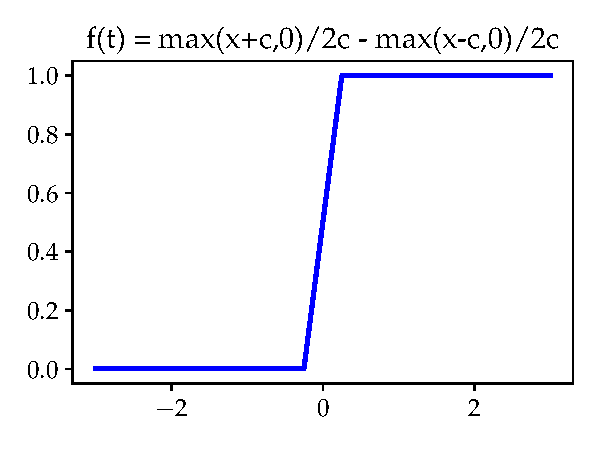
\includegraphics[width=0.5\textwidth,height=\textheight]{assets/relu2step}
\caption{Creating a step function from ReLUs. Here, c=1/4.}
\end{figure}

To see why, suppose we have a nonzero function~\(f\) that is not
well-approximated by a sum of the form \[
    \sum_{i=1}^N w_i \sigma(a_i^Tx +b_i)
\] This means that we must have \[
    \int \sigma(a^Tx +b) f(x) \mathrm{d} x =0
\] for all vectors~\(a\) and scalars~\(b\). In turn, since our
nonlinearity can approximate step functions, this implies that for
any~\(a\) and any \(t_0\) and~\(t_1\), \[
    \int \mathbb{1}\{t_0 \leq a^Tx \leq t_1\} f(x) \mathrm{d} x = 0\,.
\] We can approximate any continuous function as a sum of the indicator
function of intervals, which means \[
    \int h(a^T x) f(x) \mathrm{d} x = 0
\] for any continuous function~\(h\) and any vector~\(a\). Using
\(h(t)=\exp(it)\) proves that the Fourier transform of~\(f\) is equal to
zero, and hence that~\(f\) itself equals zero. This is a contradiction.

The core of Cybenko's argument is a reduction to approximation in one
dimension. From this perspective, it suffices to find a nonlinearity
that can well-approximate ``bump functions'' which are nearly equal to
zero outside a specified interval and are equal to~\(1\) at the center
of the interval. This opens up a variety of potential nonlinearities for
use as universal approximators.

While elegant and simple, Cybenko's argument does not tell us \emph{how
many} terms we need in our approximation. More refined work on this
topic was pursued in the 1990s. Barron\footnote{Barron, {``Universal
  Approximation Bounds for Superpositions of a Sigmoidal Function,''}
  \emph{Transactions on Information Theory} 39, no. 3 (1993): 930--45.}
used a similar argument about step functions combined with a powerful
randomized analysis due to Maurey.\footnote{Pisier, {``Remarques Sur Un
  résultat Non Publié de {B}.~{M}aurey,''} in \emph{Séminaire d'analyse
  Fonctionnelle} (Palaiseau: Ecole Polytechnique Centre de
  Mathematiques, 1980-1981).} Similar results were derived for
sinusoids\footnote{Jones, {``A Simple Lemma on Greedy Approximation in
  {H}ilbert Space and Convergence Rates for Projection Pursuit
  Regression and Neural Network Training,''} \emph{Annals of Statistics}
  20, no. 1 (1992): 608--13.} by Jones and ReLU networks\footnote{Breiman,
  {``Hinging Hyperplanes for Regression, Classification, and Function
  Approximation,''} \emph{Transactions on Information Theory} 39, no. 3
  (1993): 999--1013.} by Breiman. All of these results showed that
two-layer networks sufficed for universal approximation, and quantified
how the number of basis functions required scaled with respect to the
complexity of the approximated function.

\hypertarget{random-features}{%
\subsection{Random features}\label{random-features}}

\index{random features}

Though the idea seems a bit absurd, a powerful means of choosing basis
function is by random selection. Suppose we have a parametric family of
basis functions~\(b(x;\vartheta)\). A random feature map chooses
\(\vartheta_1,\ldots,\vartheta_D\) from some distribution
on~\(\vartheta\), and use the feature map \[
    \Phi_{\text{rf}}(x) = \begin{bmatrix}
        b(x;\vartheta_1) \\b(x;\vartheta_2)\\ \vdots \\b(x;\vartheta_D)
    \end{bmatrix}\,.
\] The corresponding prediction functions are of the form \[
    f(x) = \sum_{k=1}^{D} w_k b(x;\vartheta_k)
\] which looks very much like a neural network. The main difference is a
matter of emphasis: here we are stipulating that the parameters
\(\vartheta_k\) are random variables, whereas in neural networks,
\(\vartheta_k\) would be considered parameters to be determined by the
particular function we aim to approximate.

Why might such a random set of functions work well to approximate
complex functional behavior? First, from the perspective of
optimization, it might not be too surprising that a random set of
nonlinear basis functions will be linearly independent. Hence, if we
choose enough of them, we should be able to fit any set of desired
labels.

Second, random feature maps are closely connected with kernel spaces.
The connections were initially drawn out in work by Rahimi and
Recht.\footnote{Rahimi and Recht, {``Random Features for Large-Scale
  Kernel Machines,''} in \emph{Advances in Neural Information Processing
  Systems}, 2007; Rahimi and Recht, {``Weighted Sums of Random Kitchen
  Sinks: Replacing Minimization with Randomization in Learning,''} in
  \emph{Advances in Neural Information Processing Systems}, 2008.} Any
random feature map generates an empirical kernel,
\(\Phi_{\text{rf}}(x)^T \Phi_{\text{rf}}(z)\). The expected value of
this kernel can be associated with some Reproducing Kernel Hilbert
Space. \[
\begin{aligned}
\mathop\mathbb{E}[\tfrac{1}{D} \Phi_{\text{rf}}(x)^T \Phi_{\text{rf}}(z) ]
&= \mathop\mathbb{E}\left[\frac{1}{D} \sum_{k=1}^D b(x;\vartheta_k) b(z;\vartheta_k) \right]\\
&= \mathop\mathbb{E}[b(x;\vartheta_1) b(z;\vartheta_1) ]\\
& = \int p(\vartheta) b(x;\vartheta) b(z;\vartheta) \mathrm{d}\vartheta
\end{aligned}
\] In expectation, the random feature map yields a kernel equal given by
the final integral expressions. There are many interesting kernels that
can be written as such an integral. In particular, the Gaussian kernel
would arise if \[
\begin{aligned}
p(\vartheta) &= \mathcal{N}(0,\gamma I)\\
b(x;\vartheta) &= [\cos(\vartheta^T x), \,\, \sin(\vartheta^T x)]
\end{aligned}
\] To see this, recall that the Fourier transform of a Gaussian is a
Gaussian, and write: \[
\begin{aligned}
    k(x,z) &= \exp(-\tfrac{\gamma}{2} \Vert x-z \Vert^2)\\
    &= \frac{1}{(2 \pi \gamma)^{d/2}}\int \exp \left(-\frac{ \Vert v\Vert^2}{2\gamma}\right) \exp(i v^T(x-z)) \mathrm{d} v\\
    &= \frac{1}{(2 \pi \gamma)^{d/2}}\int \exp \left(-\frac{ \Vert v\Vert^2}{2\gamma}\right) \left\{\cos(v^T x) \cos(v^Tz) + \sin(v^T x)\sin(v^Tz)\right\} \mathrm{d} v\,.
\end{aligned}
\] This calculation gives new insights into the feature space associated
with a Gaussian kernel. It shows that the Gaussian kernel is a
continuous mixture of inner products of sines and cosines. The sinusoids
are weighted by a Gaussian function on their frequency: high frequency
sinusoids have vanishing weight in this expansion. The parameter
\(\gamma\) controls how quickly the higher frequencies are damped.
Hence, the feature space here can be thought of as low frequency
sinusoids. If we sample a frequency from a Gaussian distribution, it
will be low frequency (i.e., have small norm) with high probability.
Hence, a random collection of low frequency sinusoids approximately
spans the same space as that spanned by a Gaussian kernel.

If instead of using sinusoids, we chose our random features to be
\(\mathrm{ReLU}(v^Tx)\), our kernel would become \[
\begin{aligned}
    k(x,z)
    &= \frac{1}{(2 \pi)^{d/2}}\int \exp \left(-\frac{ \Vert v\Vert^2}{2}\right)\operatorname{ReLU}(v^T x)\operatorname{ReLU}(v^T z) \mathrm{d} v\\
    &= \Vert x\Vert \Vert z\Vert \left\{sin(\vartheta) + (\pi-\vartheta) \cos(\vartheta)\right\}\,,
\end{aligned}
\] where \[
        \vartheta = \cos^{-1} \left(\frac{\langle x, z \rangle}{\Vert x \Vert \Vert z \Vert}\right)\,.
\] This computation was first made by Cho and Saul.\footnote{Cho and
  Saul, {``Kernel Methods for Deep Learning,''} in \emph{Advances in
  Neural Information Processing Systems}, 2009.} Both the Gaussian
kernel and this ``ReLU kernel'' are universal Taylor kernels, and, when
plotted, we see even are comparable on unit norm data.

\begin{figure}
\centering
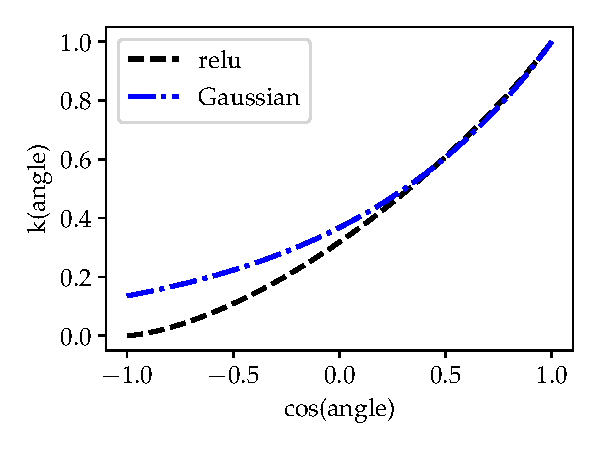
\includegraphics[width=0.75\textwidth,height=\textheight]{assets/kernel_compare}
\caption{Comparison of the Gaussian and Arccosine Kernels. Plotting the
kernel value as a function of the angle between two unit norm vectors.}
\end{figure}

Prediction functions built with random features are just randomly wired
neural networks. This connection is useful for multiple reasons. First,
as we will see in the next chapter, optimization of the weights~\(w_k\)
is far easier than joint optimization of the weights and the parameters
\(\vartheta\). Second, the connection to kernel methods makes the
generalization properties random features straightforward to analyze.
Third, much of the recent theory of neural nets is based on connections
between random feature maps and the randomization at initialization of
neural networks. The main drawback of random features is that, in
practice, they often require large dimensions before they provide
predictions on par with neural networks. These tradeoffs are worth
considering when designing and implementing nonlinear prediction
functions.

Returning to the radial basis expansion \[
    f(x) = \sum_{j=1}^k w_k  e^{-\gamma \Vert x-z_j \Vert^2}\,,
\] we see that this expression could be a neural network, a kernel
machine, or a random feature network. The main distinction between these
three methods is how the~\(z_j\) are selected. Neural nets search
require some sort of optimization procedure to find the~\(z_j\). Kernel
machines place the~\(z_j\) on the training data. Random features
select~\(z_j\) at random. The best choice for any particular prediction
problem will always be dictated by the constraints of practice.

\hypertarget{chapter-notes-3}{%
\section{Chapter notes}\label{chapter-notes-3}}

To our knowledge, there is no full and holistic accounting of
measurement and quantization, especially when that quantization is
motivated by data science applications. From the statistical signal
processing viewpoint, we have a full and complete theory of quantization
in terms of understanding what signals can be reconstructed from digital
measurements. The Nyquist-Shannon theory allows us to understand what
parts of signals may be lost and what artifacts are introduced. Such
theory is now canon in undergraduate courses on signal processing (See,
e.g., Oppenheim and Willsky).\footnote{Oppenheim, Willsky, and Nawab,
  \emph{Signals and Systems} (Prentice-Hall International, 1997).} For
task-driven sampling, the field remains quite open. The theory of
compressive sensing led to many recent and exciting developments in this
space, showing that task-driven sampling where we combined domain
knowledge, computation, and device design could reduce the data
acquisition burdens of many pattern recognition tasks.\footnote{Candès
  and Wakin, {``An Introduction to Compressive Sampling,''} \emph{{IEEE}
  Signal Processing Magazine} 25, no. 2 (2008): 21--30.} The theory of
experiment design and survey design has taken some cues from task-driven
sampling, but active research aims to understand how to best collect
data to that respects privacy promotes equity, and maximizes benefit.

Reproducing kernels have been used in pattern recognition and machine
learning for nearly as long as neural networks. Kernels and Hilbert
spaces were first used in time series prediction in the late 1940s, with
fundamental work by Karhunen--Loève showing that the covariance function
of a time series was a Mercer Kernel.\footnote{Karhunen, {``{Ü}ber
  Lineare Methoden in Der Wahrscheinlichkeitsrechnung,''} \emph{Annales
  Academia Scientiarum Fennica Mathematica, Series A}, no. 37 (1947):
  1--47; Loève, {``Functions Aleatoire de Second Ordre,''} \emph{Revue
  Science} 84 (1946): 195--206.} Shortly thereafter, Reproducing Kernel
Hilbert Spaces were formalized by Aronszajn in 1950.\footnote{Aronszajn,
  {``Theory of Reproducing Kernels,''} \emph{Transactions of the
  American Mathematical Society} 68, no. 3 (1950): 337--404.} Parzen was
likely the first to show that time series prediction problem could be
reduced to solving a least-squares problem in an RKHS and hence could be
computed by solving a linear system.\footnote{Parzen, {``An Approach to
  Time Series Analysis,''} \emph{The Annals of Mathematical Statistics}
  32, no. 4 (1961): 951--89.} Wahba's survey of RKHS techniques in
statistics covers many other developments post-Parzen.\footnote{Wahba,
  \emph{Spline Models for Observational Data} (Philadelphia,
  Pennsylvania: Society for Industrial; Applied Mathematics, 1990).} For
further reading on the theory and application of kernels in machine
learning consult the texts by Schölkopf and Smola\footnote{Schölkopf and
  Smola, \emph{Learning with Kernels: Support Vector Machines,
  Regularization, Optimization, and Beyond} (Cambridge: MIT Press,
  2002).} and Shawe-Taylor and Cristianini.\footnote{Shawe-Taylor and
  Cristianini, \emph{Kernel Methods for Pattern Analysis} (Cambridge
  university press, 2004).}

Also since its inception, researchers have been fascinated by the
approximation power of neural networks. Rosenblatt discussed properties
of universal approximation in his monograph on neurodynamics.\footnote{Rosenblatt,
  {``Principles of Neurodynamics.''}} It was in the 80s when it became
clear that though neural networks were able to approximate any
continuous function, they needed to be made more complex and intricate
in order to achieve high quality approximation. Cybenko provided a
simple proof that neural nets were dense in the space of continuous
functions, though did not estimate how large such networks might need to
be.\footnote{Cybenko, {``Approximation by Superpositions of a Sigmoidal
  Function.''}} An elegant, randomized argument by Maurey\footnote{Pisier,
  {``Remarques Sur Un résultat Non Publié de {B}.~{M}aurey.''}} led to a
variety of approximation results which quantified how many basis terms
were needed. Notably, Jones showed that a simple greedy method could
approximate any continuous function with a sum of sinusoids.\footnote{Jones,
  {``A Simple Lemma on Greedy Approximation in {H}ilbert Space and
  Convergence Rates for Projection Pursuit Regression and Neural Network
  Training.''}} Barron shows that similar greedy methods could be
used\footnote{Barron, {``Universal Approximation Bounds for
  Superpositions of a Sigmoidal Function.''}} to build neural nets that
approximated any function. Breiman analyzed ReLU networks using the same
framework.\footnote{Breiman, {``Hinging Hyperplanes for Regression,
  Classification, and Function Approximation.''}} The general theory of
approximation by bases is rich, and a Pinkus' book details some of the
necessary and sufficient conditions to achieve high quality
approximations with as few bases as possible.\footnote{Pinkus,
  \emph{N-Widths in Approximation Theory} (New York: Springer, 1985).}

That randomly wired neural networks could solve pattern recognition
problems also has a long history. Minsky's first electronic neural
network, SNARC, was randomly wired\footnote{The story of SNARC
  (Stochastic Neural Analog Reinforcement Calculator) is rather
  apocryphal. There are no known photographs of the assembled device,
  though this article has a picture of one of the ``neurons'':
  https://www.the-scientist.com/foundations/machine--learning--1951-65792
  The commonly referenced publication, a Harvard technical report,
  appears to not be published. However, the ``randomly wired'' story
  lives on, and it is one that Minsky told countless times through his
  life.}. Many years later, Rahimi and Recht built upon the
approximation theory of Maurey, Barron, and Jones to show that random
combinations of basis functions could well-approximate continuous
functions, and that such random combinations could be thought of as
approximately solving prediction problems in an RKHS.\footnote{Rahimi
  and Recht, {``Weighted Sums of Random Kitchen Sinks''}; Rahimi and
  Recht, {``Random Features for Large-Scale Kernel Machines''}; Rahimi
  and Recht, {``Uniform Approximation of Functions with Random Bases,''}
  in \emph{The \(46\)Th Annual Allerton Conference on Communication,
  Control, and Computing}, 2008.} This work was later used as a means to
understand neural networks, and, in particular, the influence of their
random initializations. Daniely et al.~computed the kernel spaces
associated with that randomly initialized neural networks,\footnote{Daniely,
  Frostig, and Singer, {``Toward Deeper Understanding of Neural
  Networks: The Power of Initialization and a Dual View on
  Expressivity,''} in \emph{Advances in Neural Information Processing
  Systems}, 2016.} and Jacot et al.~pioneered a line of work using
kernels to understand the dynamics of neural net training.\footnote{Jacot,
  Gabriel, and Hongler, {``Neural Tangent Kernel: Convergence and
  Generalization in Neural Networks,''} in \emph{Advances in Neural
  Information Processing Systems}, 2018, 8580--89.}

There has been noted cultural tension between the neural-net and kernel
``camps.'' For instance, the tone of the introduction of work by Decoste
and Schölkopf telegraphs a disdain by neural net proponents of the
Support Vector Machine.\footnote{Decoste and Schölkopf, {``Training
  Invariant Support Vector Machines,''} \emph{Machine Learning} 46, no.
  1--3 (2002): 161--90.}

\begin{quote}
Initially, SVMs had been considered a theoretically elegant spin-off of
the general but, allegedly, largely useless VC-theory of statistical
learning. In 1996, using the first methods for incorporating prior
knowledge, SVMs became competitive with the state of the art in the
handwritten digit classification benchmarks that were popularized in the
machine learning community by AT\&T and Bell Labs. At that point,
practitioners who are not interested in theory, but in results, could no
longer ignore SVMs.
\end{quote}

With the rise of deep learning, however, there are a variety of machine
learning benchmarks where SVMs or other kernel methods fail to match the
performance of neural networks. Many have dismissed kernel methods as a
framework whose time has past. However, kernels play an evermore active
role in helping to better understand neural networks and insights from
deep learning have helped to improve the power of kernel methods on
pattern recognition tasks.\footnote{Shankar et al., {``Neural Kernels
  Without Tangents,''} in \emph{International Conference on Machine
  Learning}, 2020.} Neural nets and kernels are complementary, and
active research in machine learning aims to bring these two views more
closely together.

\chapter{Optimization}

In decision theory, we devised a closed form expression for the optimal
decision rule assuming we have a probability model for the data. Then we
turned to empirical risk minimization (ERM) where we instead rely on
numerical methods to discover good decision rules when we don't have
such a probability model. In this chapter, we take a closer look at how
to solve empirical risk minimization problems effectively. We focus on
the core optimization methods commonly used to solve empirical risk
minimization problems and on the mathematical tools used to analyze
their running times.

Our main subject will be \emph{gradient descent} algorithms and how to
shape loss functions so that gradient descent succeeds. Gradient descent
is an iterative procedure that iterates among possible models, at each
step replacing the old model with one with lower empirical risk. We show
that the class of optimization problems where gradient descent is
guaranteed to find an optimal solution is the set of \emph{convex
functions}. When we turn to risk minimization, this means that gradient
descent will find the model that minimizes the empirical risk whenever
the loss function is convex and the decision function is a linear
combination of features.

We then turn to studying \emph{stochastic} gradient descent, the
workhorse of machine learning. Stochastic gradient descent is
effectively a generalization of the perceptron learning rule. Its
generality enables us to apply it to a variety of function classes and
loss functions and guarantee convergence even if the data may not be
separable. We spend a good deal of time looking at the dynamics of the
stochastic gradient method to try to motivate why it is so successful
and popular in machine learning.

Starting from the convex case, we work towards more general nonconvex
problems. In particular, we highlight two salient features of gradient
descent and stochastic gradient descent that are particular to empirical
risk minimization and help to motivate the resilience of these methods.

First, we show that even for problems that are not convex, gradient
descent for empirical risk minimization has an \emph{implicit convexity}
property that encourages convergence. Though we explicitly optimize over
function representations which are computationally intractable to
optimize in the worst-case, it turns out that we can still reason about
the convergence of the predictions themselves.

Second, we show that gradient descent implicitly manages the complexity
of the prediction function, encouraging solutions of low complexity in
cases where infinitely many solutions exist. We close the chapter with a
discussion of other methods for empirical risk minimization that more
explicitly account for model complexity and stable convergence.

\hypertarget{optimization-basics}{%
\section{Optimization basics}\label{optimization-basics}}

Stepping away from empirical risk minimization for a moment, consider
the general minimization problem \[
\begin{array}{ll}
    \text{minimize}_w  & \Phi(w)
\end{array}
\] where~\(\Phi\colon\mathbb{R}^d\to\mathbb{R}\) is a real-valued
function over the domain \(\mathbb{R}^d\).

When and how can we minimize such a function? Before we answer this
question, we need to formally define what we're shooting for.

\begin{Definition}

A point~\(w_\star\) is a \emph{minimizer} of~\(\Phi\) if
\(\Phi(w_\star)\leq \Phi(w)\) for all~\(w\). It is a \emph{local
minimizer} of \(\Phi\) if for
some~\(\epsilon> 0\),~\(\Phi(w_\star)\leq \Phi(w)\) for all \(w\) such
that~\(\Vert w-w_\star \Vert\leq \epsilon\).

Sometimes we will refer to minimizers as \emph{global minimizers} to
contrast against local minimizers.

\end{Definition}

The figure below presents example functions and their minima. In the
first illustration, there is a unique minimizer. In the second, there
are an infinite number of minimizers, but all local minimizers are
global minimizers. In the third example, there are many local minimizers
that are not global minimizers.

\begin{figure}
\centering
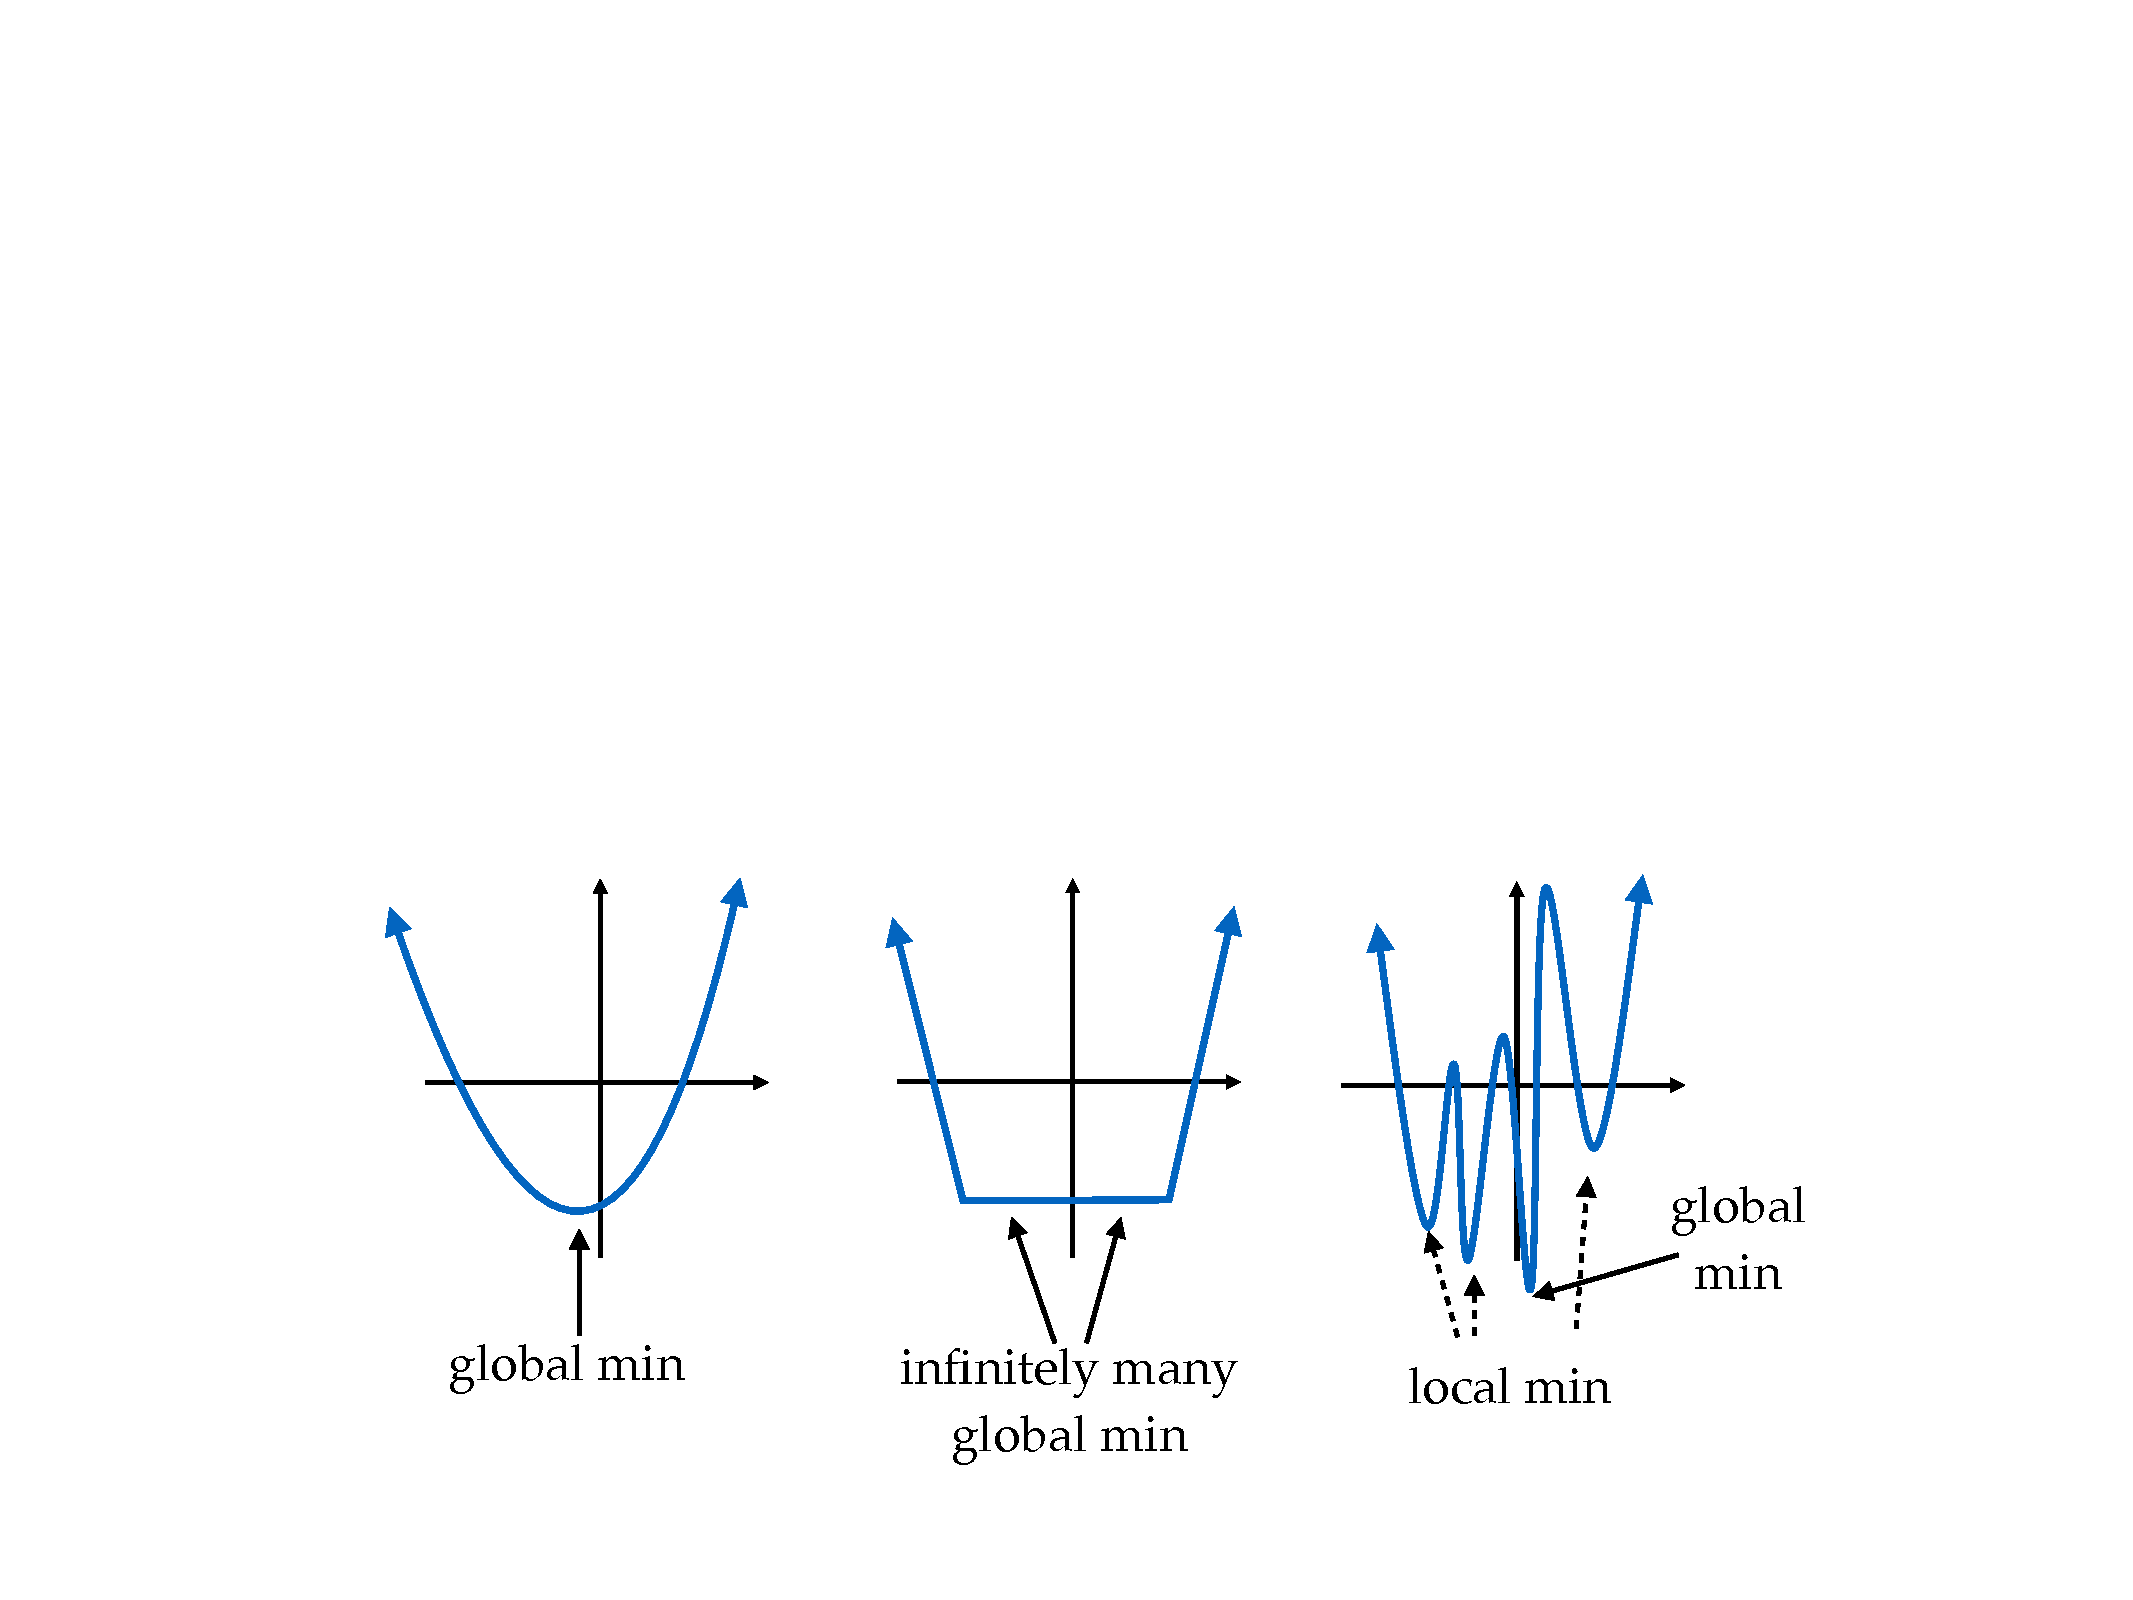
\includegraphics[width=1\textwidth,height=\textheight]{assets/minima}
\caption{Examples of minima of functions. In the first illustration,
there is a unique minimizer. In the second, there are an infinite number
of minimizers, but all local minimizers are global minimizers. In the
third example, there are many local minimizers that are not global
minimizers.}
\end{figure}

Note that in our example, the two functions without suboptimal local
minimizers share the property that for any two points~\(w_1\)
and~\(w_2\), the line segment connecting~\((w_1,\Phi(w_1))\)
to~\((w_2,\Phi(w_2))\) lies completely above the graph of the function.
Such functions are called \emph{convex functions}.

\begin{Definition}

A function~\(\Phi\) is \emph{convex} if for all~\(w_1\),~\(w_2\)
in~\(\mathbb{R}^d\) and~\(\alpha \in [0,1]\), \[
        \Phi(\alpha w_1 + (1-\alpha) w_2 )\leq \alpha\Phi(w_1)+(1-\alpha)\Phi(w_2)\,.
\]

\end{Definition}

We will see shortly that convex functions are the class of functions
where gradient descent is guaranteed to find an optimal solution.

\begin{figure}
\centering
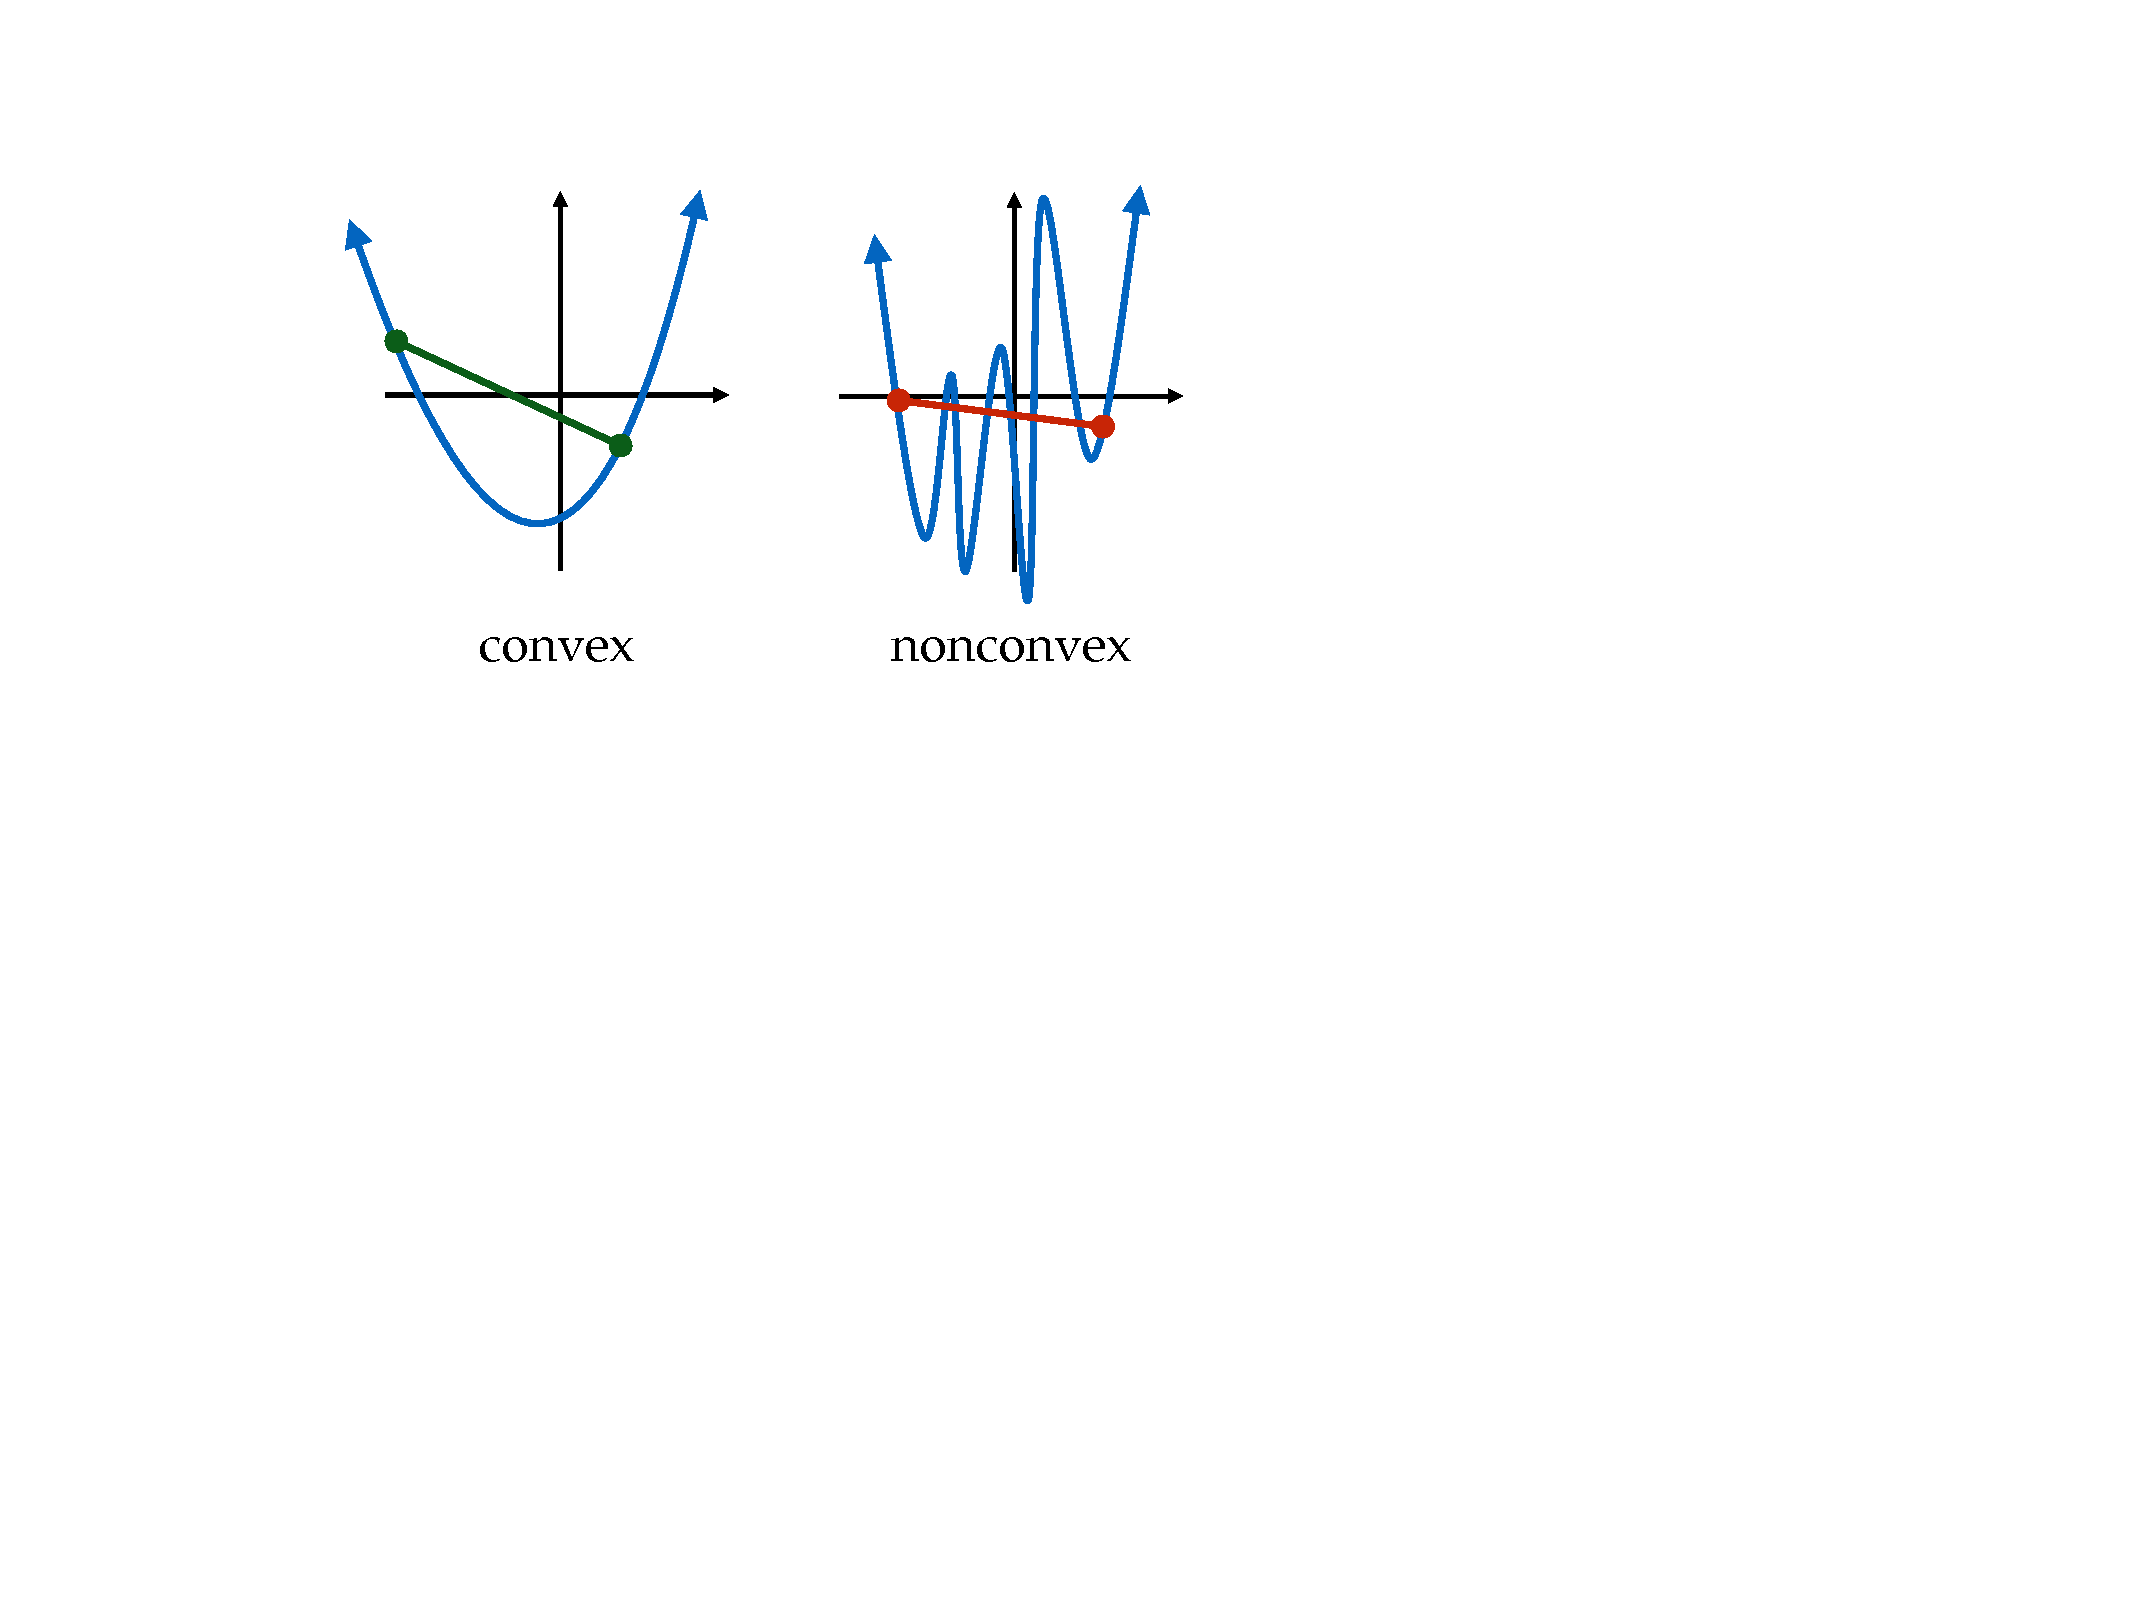
\includegraphics[width=0.66\textwidth,height=\textheight]{assets/convex}
\caption{Convex vs nonconvex functions.}
\end{figure}

\hypertarget{gradient-descent}{%
\section{Gradient descent}\label{gradient-descent}}

Suppose we want to minimize a differentiable function
\(\Phi\colon\mathbb{R}^d \rightarrow \mathbb{R}\). Most of the
algorithms we will consider start at some point~\(w_0\) and then aim to
find a new point~\(w_1\) with a lower function value. The simplest way
to do so is to find a direction~\(v\) such that~\(\Phi\) is decreasing
when moving along the direction~\(v\). This notion can be formalized by
the following definition:

\begin{Definition}

A vector~\(v\) is a \emph{descent direction} for~\(\Phi\) at~\(w_0\) if
\(\Phi(w_0 + tv) < \Phi(w_0)\) for some~\(t>0\).

\end{Definition}

For continuously differentiable functions, it's easy to tell if~\(v\) is
a descent direction: if~\(v^T \nabla \Phi(w_0) <0\) then~\(v\) is a
descent direction.

To see this note that by Taylor's theorem, \[
\Phi(w_0 + \alpha v) = \Phi(w_0) + \alpha \nabla \Phi(w_0 + \tilde{\alpha} v)^T v
\] for some~\(\tilde{\alpha} \in [0,\alpha]\). By continuity,
if~\(\alpha\) is small, we'll
have~\(\nabla \Phi(w_0 + \tilde{\alpha} v)^Tv <0\).
Therefore~\(\Phi(w_0 + \alpha v) < \Phi(w_0)\) and~\(v\) is a descent
direction.

This characterization of descent directions allows us to provide
conditions as to when~\(w\) minimizes~\(\Phi\).

\begin{Proposition}

The point~\(w_\star\) is a local minimizer only if
\(\nabla \Phi(w_\star) = 0\,.\)

\end{Proposition}

Why is this true? Well,~\(-\nabla \Phi(w_\star)\) is always a descent
direction if it's not zero. If~\(w_\star\) is a local minimum, there can
be no descent directions. Therefore, the gradient must vanish.

Gradient descent uses the fact that the negative gradient is always a
descent direction to construct an algorithm: repeatedly compute the
gradient and take a step in the opposite direction to minimize~\(\Phi\).

\begin{Algorithm}

\textbf{Gradient Descent}

\begin{itemize}
\tightlist
\item
  Start from an initial point \(w_0 \in \mathbb{R}^d.\)
\item
  At each step \(t=0,1,2,\dots\):

  \begin{itemize}
  \tightlist
  \item
    Choose a step size \(\alpha_t>0\)
  \item
    Set \(w_{t+1} = w_t - \alpha_t \nabla \Phi(w_t)\)
  \end{itemize}
\end{itemize}

\end{Algorithm}

Gradient descent terminates whenever the gradient is so small that the
iterates~\(w_t\) no longer substantially change. Note now that there can
be points where the gradient vanishes but where the function is not
minimized. For example, maxima have this property. In general, points
where the gradient vanishes are called \emph{stationary points}. It is
critically important to remember that not all stationary points are
minimizers.

\begin{figure}
\centering
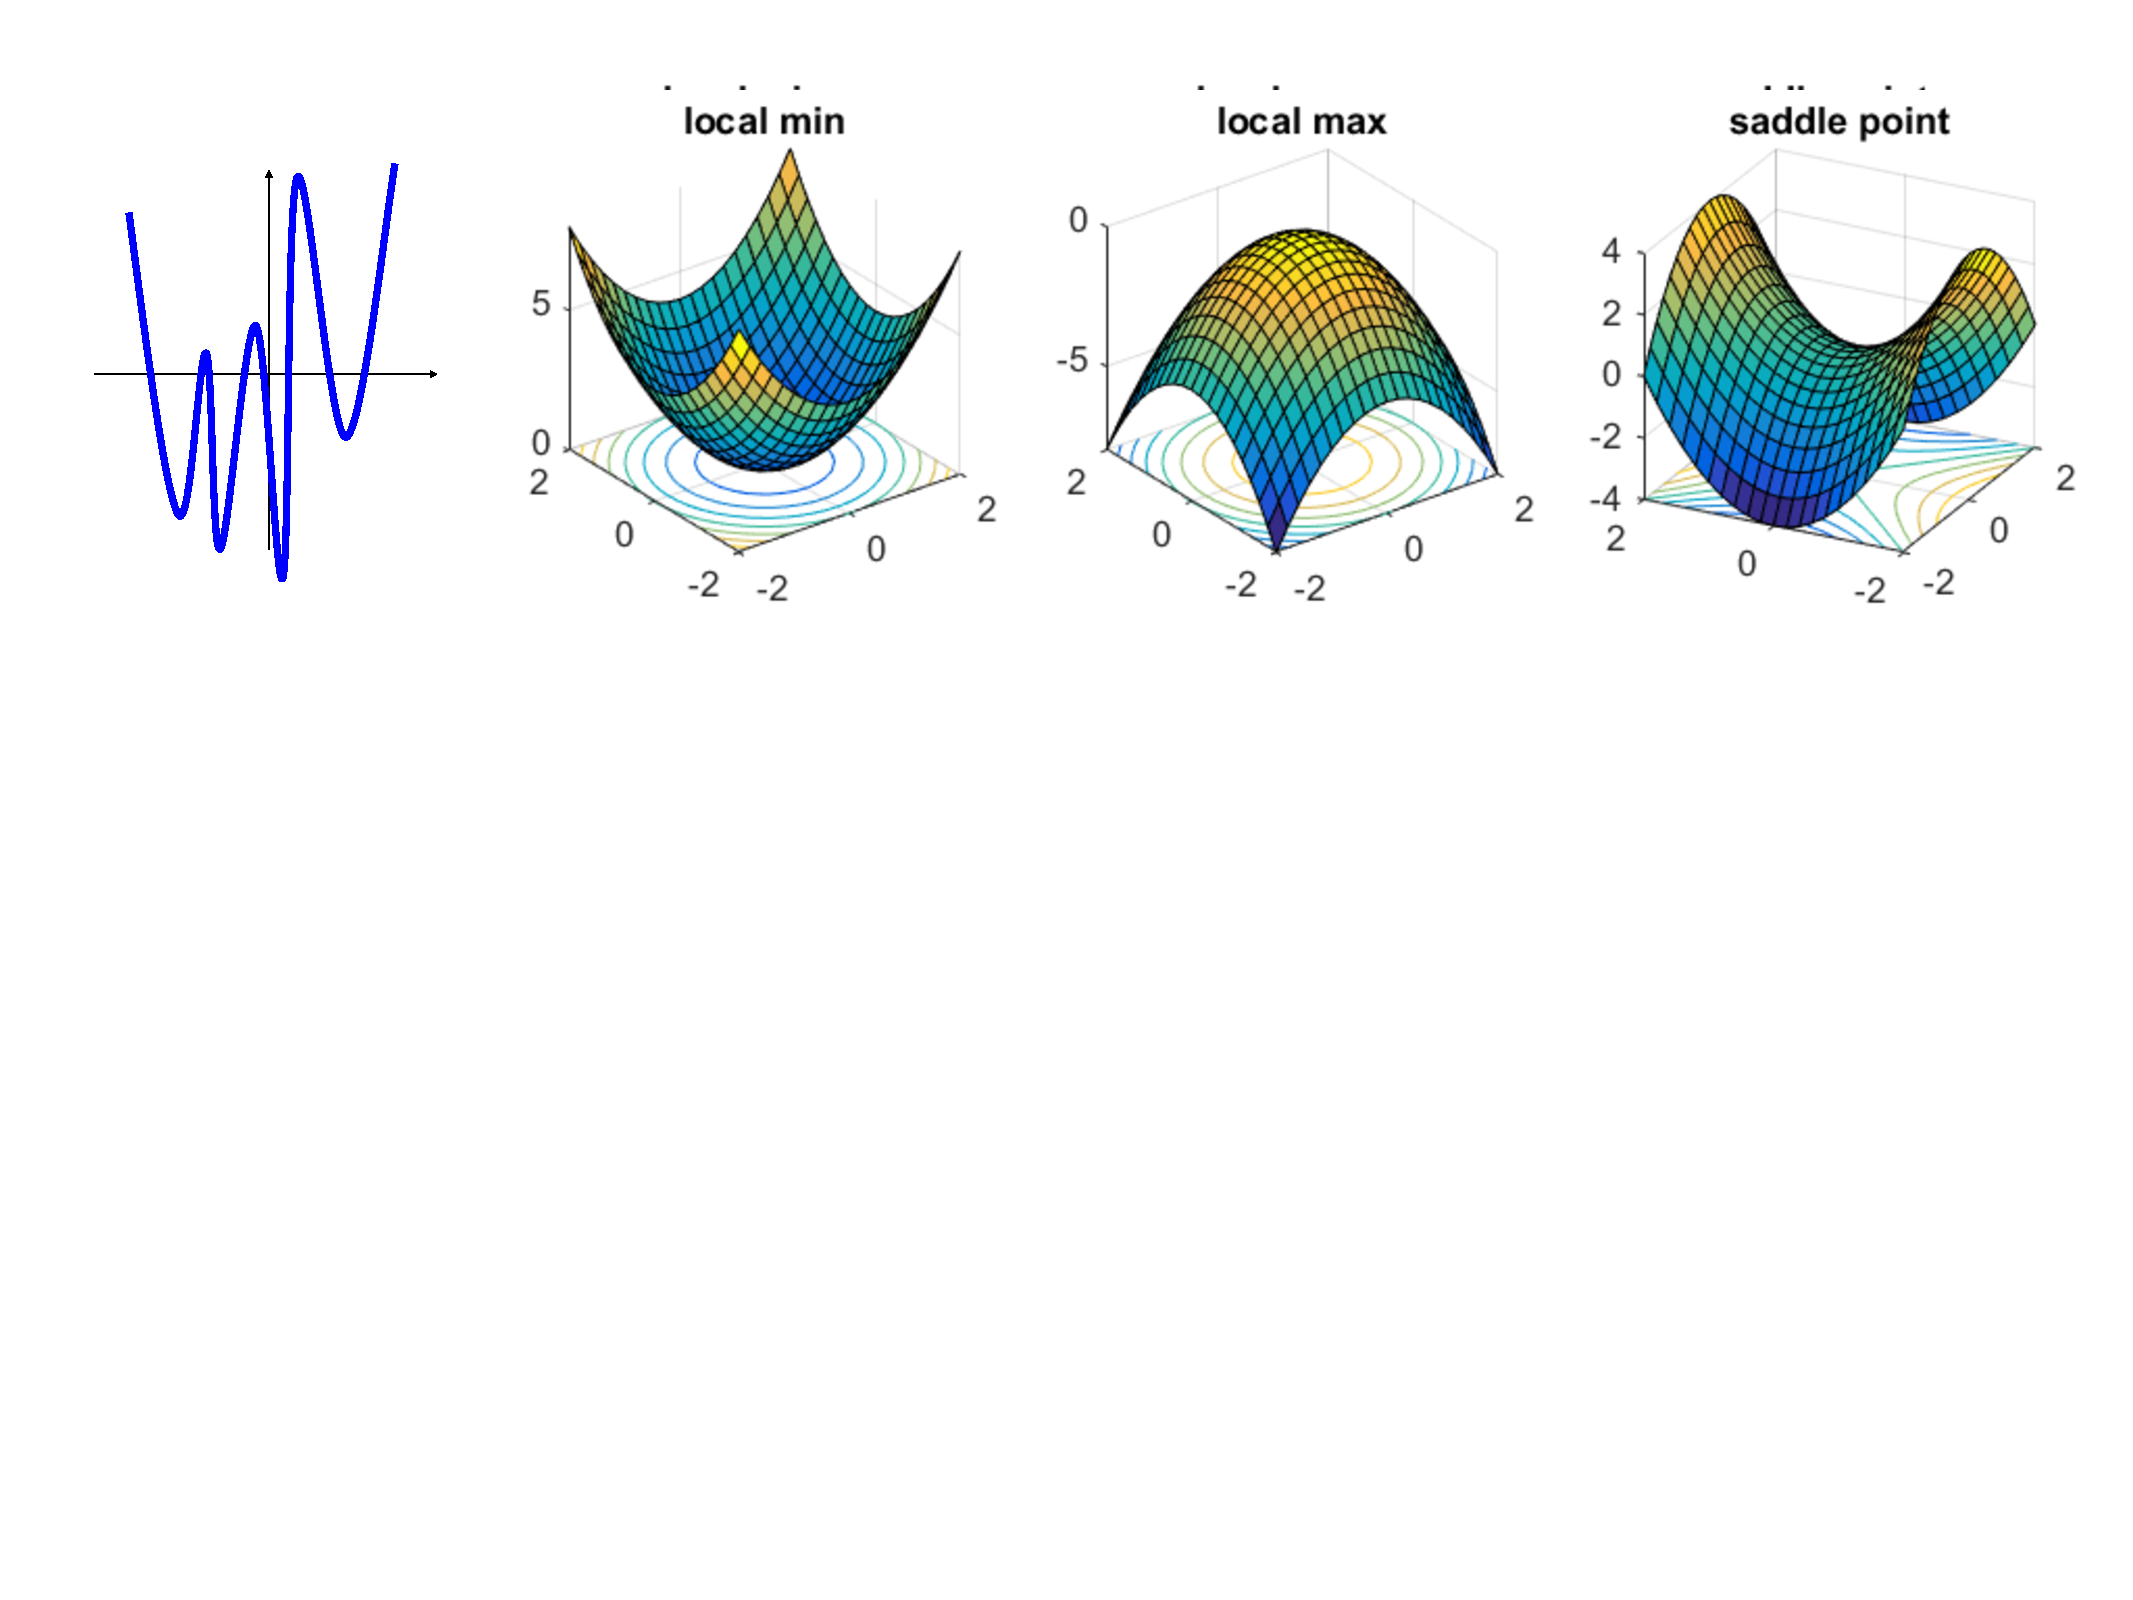
\includegraphics[width=1\textwidth,height=\textheight]{assets/stationary_points}
\caption{Examples of stationary points.}
\end{figure}

For convex~\(\Phi\), the situation is dramatically simpler. This is part
of the reason why convexity is so appealing.

\begin{Proposition}

Let~\(\Phi:\mathbb{R}^d\rightarrow \mathbb{R}\) be a differentiable
convex function. Then~\(w_\star\) is a global minimizer of~\(\Phi\) if
and only if \(\nabla \Phi(w_\star)=0\).

\end{Proposition}

\begin{Proof}

To prove this, we need our definition of convexity: for any
\(\alpha \in [0,1]\) and~\(w\in\mathbb{R}^d\), \[
    \Phi(w_\star + \alpha(w-w_\star)) =  \Phi((1-\alpha)w_\star + \alpha w) \leq (1-\alpha) \Phi(w_\star) + \alpha \Phi(w)
\] Here, the inequality is just our definition of convexity. Now, if we
rearrange terms, we have \[
    \Phi(w) \geq \Phi(w_\star) + \frac{\Phi(w_\star + \alpha(w-w_\star)) - \Phi(w_\star)}{\alpha}
\] Now apply Taylor's theorem: there is now some
\(\tilde{\alpha}\in[0,1]\) such that
\(\Phi(w_\star + \alpha(w-w_\star)) - \Phi(w_\star)=\alpha \nabla \Phi(w_\star+ \tilde{\alpha}(w-w_\star))^T(w-w_\star)\).
Taking the limit as~\(\alpha\) goes to zero yields \[
    \Phi(w) \geq \Phi(w_\star) +\nabla \Phi(w_\star)^T(w-w_\star)\,.
\]

But if~\(\nabla \Phi(w_\star)=0\), that means,
\(\Phi(w) \geq \Phi(w_\star)\) for all~\(w\), and hence~\(w_\star\) is a
global minimizer.

\end{Proof}

This last expression is quite useful and we'll record it for later.

\begin{Proposition}

Let~\(\Phi:\mathbb{R}^d\rightarrow \mathbb{R}\) be a differentiable
convex function. Then for any~\(u\) and~\(v\), we have \[
        \Phi(u) \geq \Phi(v) + \nabla \Phi(v)^T(u-v)\,.
\]

\end{Proposition}

\begin{figure}
\centering
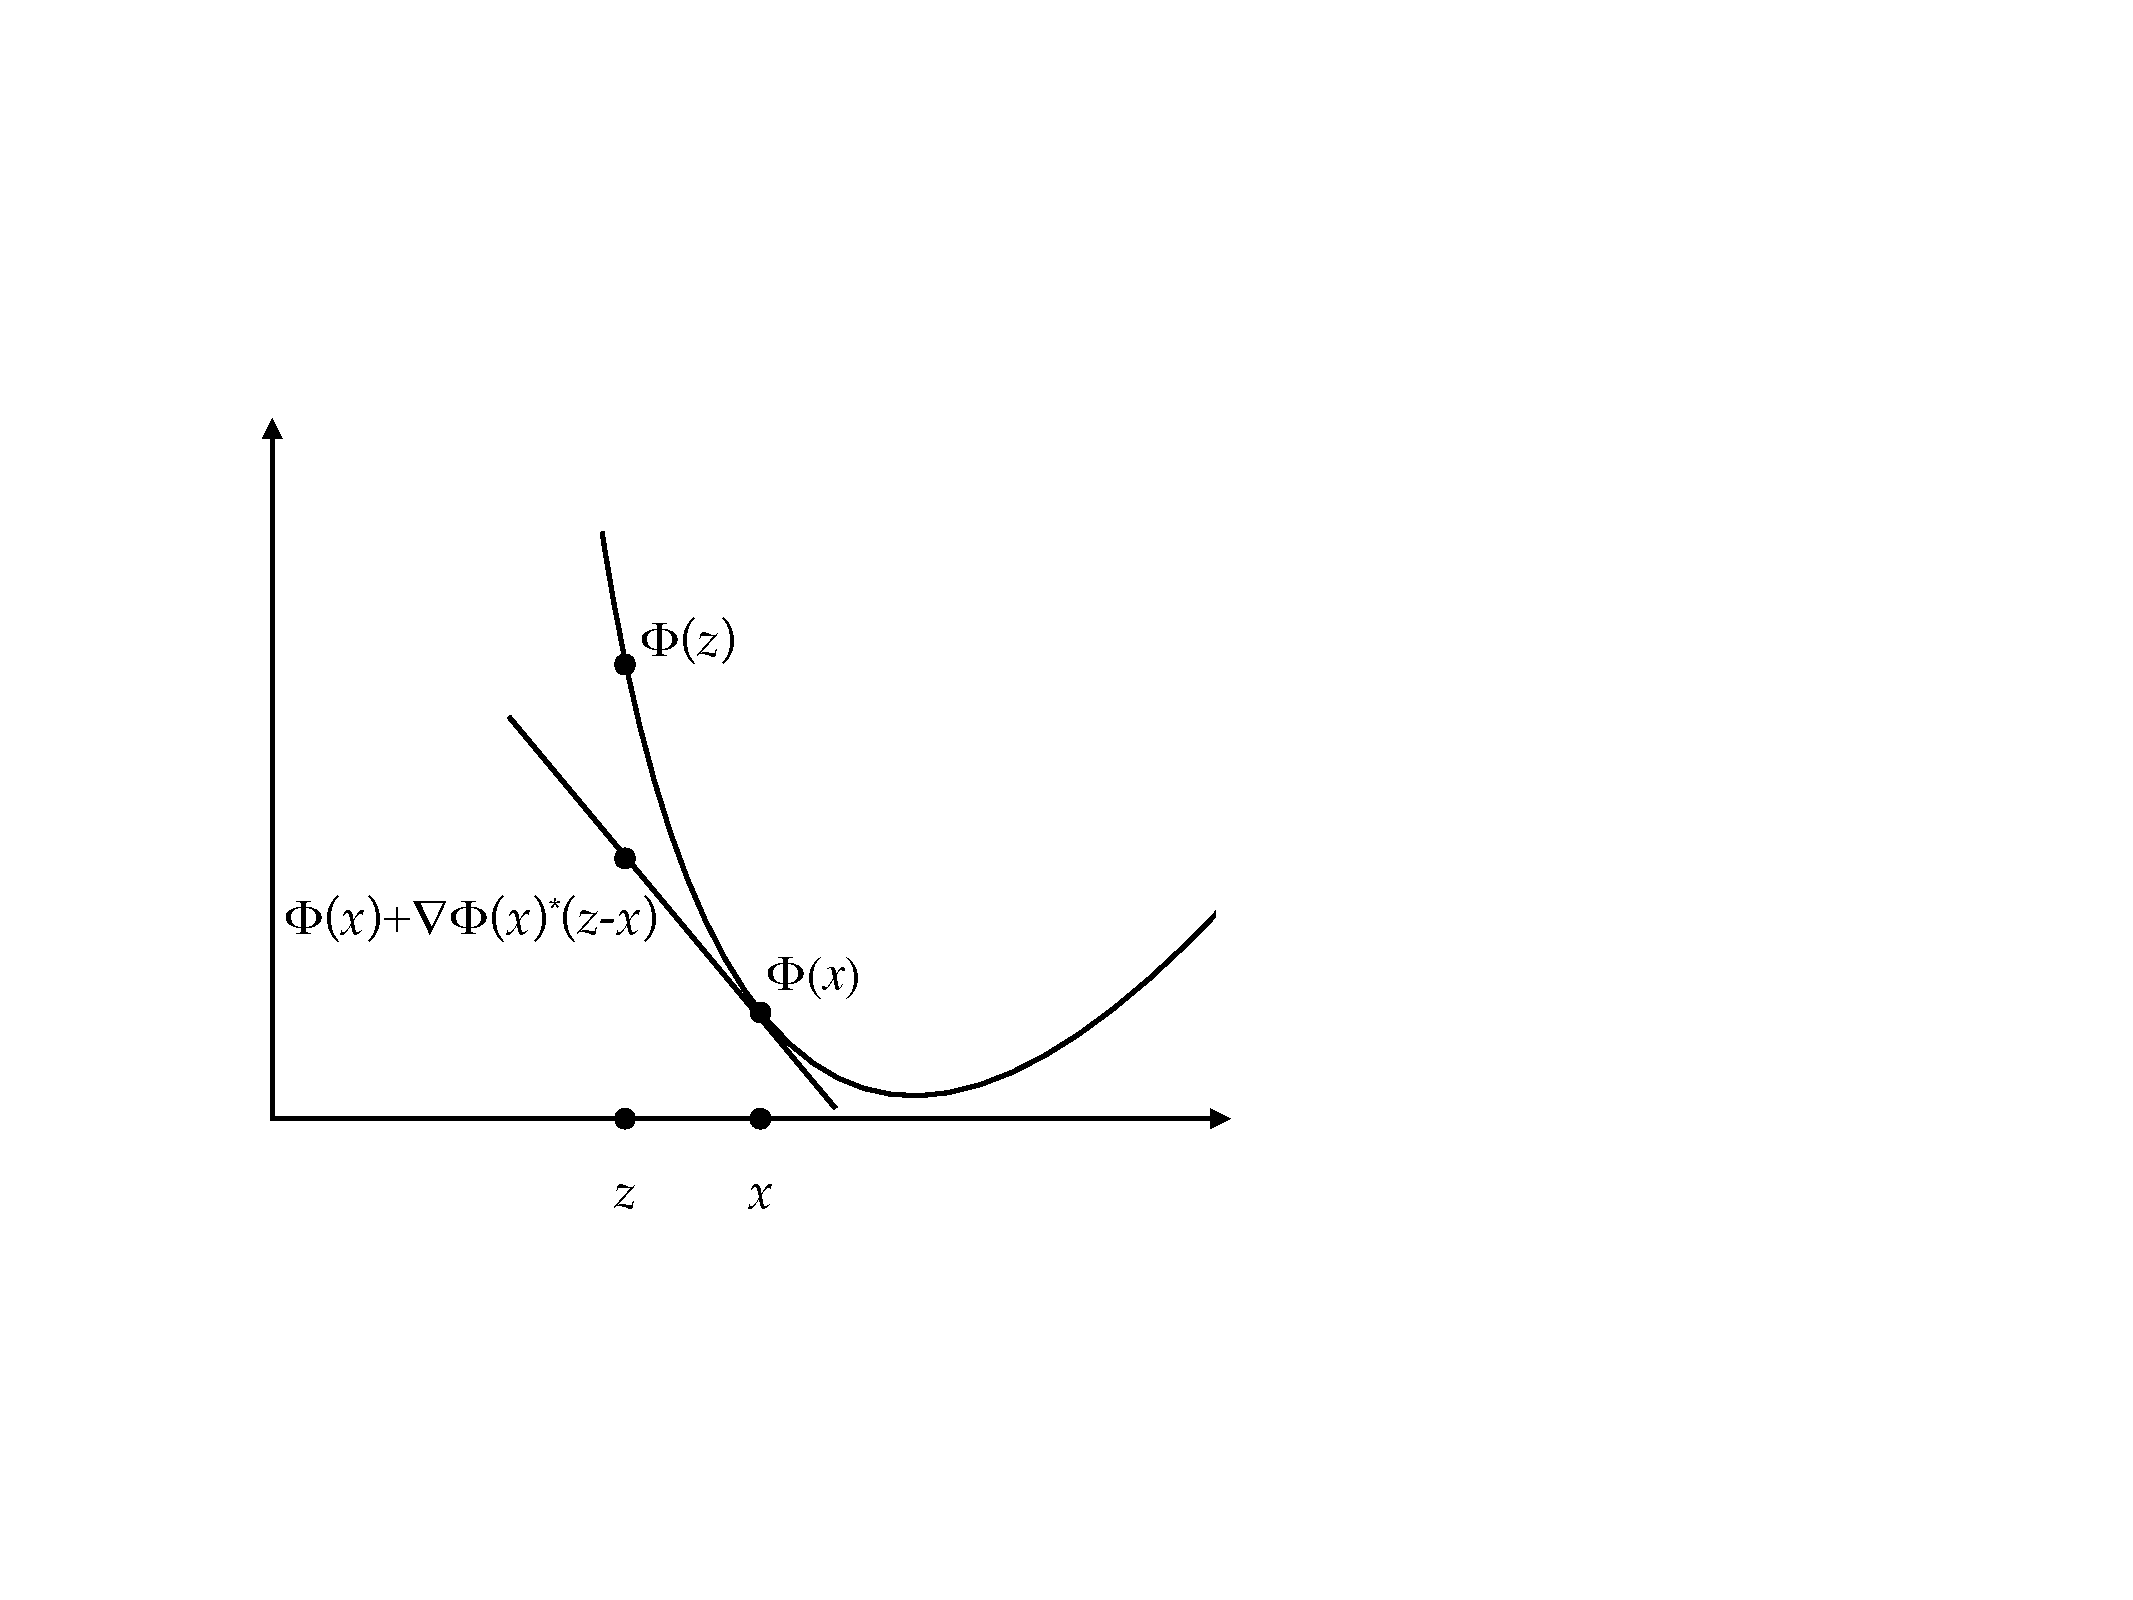
\includegraphics[width=0.6\textwidth,height=\textheight]{assets/line_below}
\caption{Tangent planes to graphs of functions are defined by the
gradient. These hyperplanes always fall below the graphs of convex
functions.}
\end{figure}

\hypertarget{a-convex-function-cookbook}{%
\subsection{A convex function
cookbook}\label{a-convex-function-cookbook}}

Testing if a function is convex seems tricky if you can't plot it. But
here are 5 rules that generate convex functions from simpler functions.
In machine learning, almost all convex cost functions are built using
these rules.

\begin{enumerate}
\def\labelenumi{\arabic{enumi}.}
\item
  All norms are convex (this follows from the triangle inequality).
\item
  If~\(\Phi\) is convex and~\(\alpha \geq 0\), then~\(\alpha \Phi\) is
  convex.
\item
  If~\(\Phi\) and~\(\Psi\) are convex, then~\(\Phi+\Psi\) is convex.
\item
  If~\(\Phi\) and~\(\Psi\) are convex, then
  \(h(w) = \max \{\Phi(w),\Psi(w)\}\) is convex.
\item
  If~\(\Phi\) is convex and~\(A\) is a matrix and~\(b\) is a vector,
  then the function~\(h(w)=\Phi(Aw+b)\) is convex.
\end{enumerate}

All of these properties can be verified using only the definition of
convex functions. For example, consider the 4th property. This is
probably the trickiest of the list. Take two points~\(w_1\) and~\(w_2\)
and \(\alpha \in [0,1]\). Suppose, without loss of generality, that
\(\Phi((1-\alpha)w_1+ \alpha w_2) \geq \Psi((1-\alpha) w_1 + \alpha w_2)\)
\[
\begin{aligned}
    h((1-\alpha) w_1 + \alpha w_2) &= \max \{\Phi((1- \alpha) w_1+ \alpha w_2),\Psi((1-\alpha) w_1 + \alpha w_2)\}\\
    &= \Phi((1-\alpha) w_1+ \alpha w_2)\\
    & \leq  (1-\alpha) \Phi(w_1)+ \alpha \Phi(w_2)\\
    &\leq (1-\alpha) \max\{\Phi(w_1),\Psi(w_1)\} + \alpha \max\{\Phi(w_2),\Psi(w_2)\}\\
    & = (1-\alpha) h(w_1) + \alpha h(w_2)
\end{aligned}
\] Here, the first inequality follows because~\(\Phi\) is convex.
Everything else follows from the definition that~\(h\) is the max of
\(\Phi\) and~\(\Psi\). The reader should verify the other four
assertions as an exercise. Another useful exercise is to verify that the
SVM cost in the next section is convex by just using these five basic
rules.

\hypertarget{applications-to-empirical-risk-minimization}{%
\section{Applications to empirical risk
minimization}\label{applications-to-empirical-risk-minimization}}

For decision theory problems, we studied the loss function that counts
errors:\marginnote{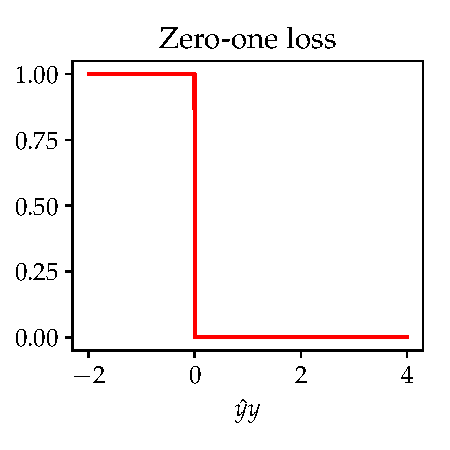
\includegraphics{assets/zeroone_loss}} \[
    \mathit{loss}(\hat{y},y) = \mathbb{1}\{ y\hat{y} \geq 0\}
\] Unfortunately, this loss is not useful for the gradient method. The
gradient is zero almost everywhere. As we discussed in the chapter on
supervised learning, machine learning practice always turns to surrogate
losses that are easier to optimize. Here we review three popular
choices, all of which are convex loss functions.\index{loss!zero-one}

Each choice leads to a different important optimization problem that has
been studied in its own right.

\hypertarget{the-support-vector-machine}{%
\subsection{The support vector
machine}\label{the-support-vector-machine}}

\index{support vector machine}\index{loss!hinge}

Consider the canonical problem of support vector machine classification.
We are provided pairs~\(\left(x_{i},y_{i}\right)\), with
\(x_{i}\in\mathbb{R}^{d}\) and~\(y_{i}\in\left\{ -1,1\right\}\) for
\(i=1,\ldots n\) (Note, the~\(y\) labels are now in~\(\{-1,1\}\) instead
of \(\{0,1\}\).) The goal is to find a vector~\(w\in \mathbb{R}^d\) such
that: \[
\begin{aligned}
w^{T}x_{i} & >  0\quad\text{ for }y_{i}=1\\
w^{T}x_{i} & < 0\quad\text{ for }y_{i}=-1
\end{aligned}
\] Such a~\(w\) defines a half-space where we believe all of the
positive examples lie on one side and the negative examples on the
other.

Rather than classifying these points exactly, we can allow some slack.
We can pay a penalty of~\(1-y_i w^T x_i\) points that are not strongly
classified. This motivates the hinge
loss\marginnote{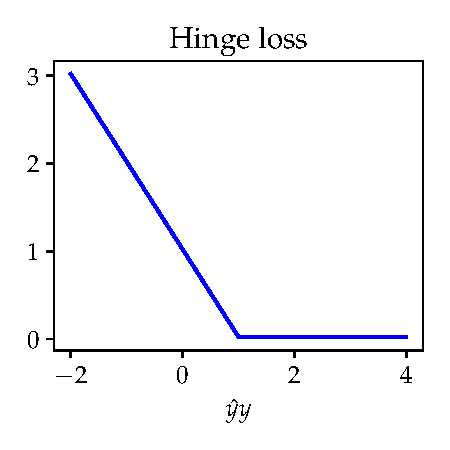
\includegraphics{assets/hinge_loss}} we encountered
earlier and leads to the \emph{support vector machine objective}: \[
    \text{minimize}_w\quad  \sum_{i=1}^n \max\left\{1-y_i w^T x_i,0\right\} \,.
\]

Defining the function~\(e(z) = \mathbb{1}\{ z\leq 1 \},\) we can compute
that the gradient of the SVM cost is \[
    -\sum_{i=1}^n e(y_i w^T x_i) y_i x_i \,.
\] Hence, gradient descent for this ERM problem would follow the
iteration \[
    w_{t+1} = w_t + \alpha \sum_{i=1}^n e(y_i w^T x_i) y_i x_i
\] Although similar, note that this isn't quite the perceptron method
yet. The time to compute one gradient step is~\(O(n)\) as we sum over
all \(n\) inner products. We will soon turn to the stochastic gradient
method that has constant iteration complexity and will subsume the
perceptron algorithm.

\hypertarget{logistic-regression}{%
\subsection{Logistic regression}\label{logistic-regression}}

\index{logistic regression}\index{loss!logistic}

Logistic regression is equivalent to using the loss
function\marginnote{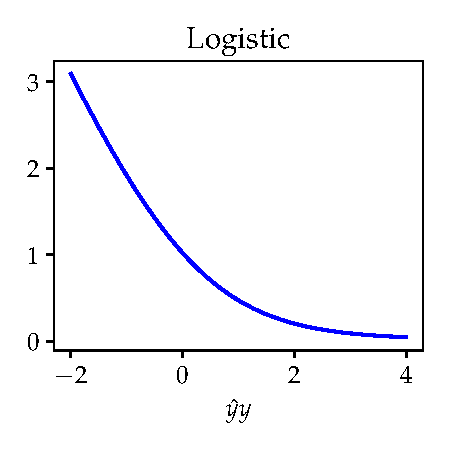
\includegraphics{assets/logistic_loss}} \[
\mathit{loss}(\hat y,y) = \log \left(1+\exp(-y\hat y)\right)\,.
\] Note that even though this loss has a probabilistic interpretation,
it can also just be seen as an approximation to the error-counting
zero-one loss.

\hypertarget{least-squares-classification}{%
\subsection{Least squares
classification}\label{least-squares-classification}}

\index{least squares}\index{loss!squared}

Least squares classification uses the loss
function\marginnote{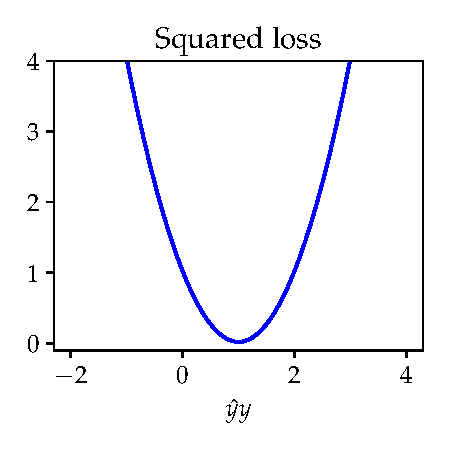
\includegraphics{assets/squared_loss}} \[
\mathit{loss}(\hat y,y) =  \tfrac{1}{2}(\hat y-y)^2\,.
\] Though this might seem like an odd approximation to the
error-counting loss, it leads to the maximum a posteriori (MAP) decision
rule when minimizing the population risk. Recall the MAP rule selects
the label that has highest probability conditional on the observed
data.\index{MAP}\index{maximum a posteriori}

It is helpful to keep the next picture in mind that summarizes how each
of these different loss functions approximate the zero-one loss. We can
ensure that the squared loss is an upper bound on the zero-one loss by
dropping the factor~\(1/2.\)

\begin{figure}
\centering
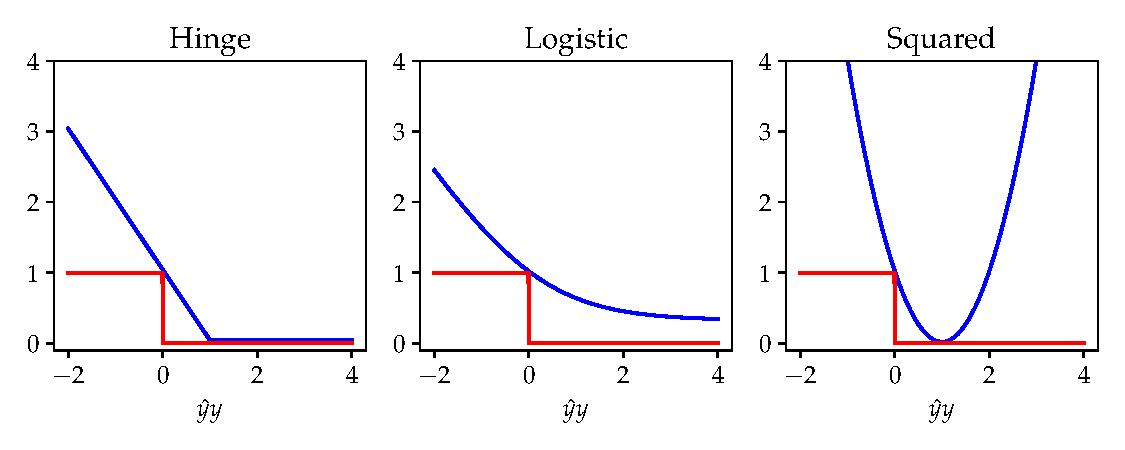
\includegraphics{assets/losses_vs_zeroone}
\caption{Example loss functions for classification. The zero-one loss is
plotted in red for comparison.}
\end{figure}

\hypertarget{insights-on-convergence-of-gradient-methods-from-quadratic-functions}{%
\section{Insights on convergence of gradient methods from quadratic
functions}\label{insights-on-convergence-of-gradient-methods-from-quadratic-functions}}

Quadratic functions are the prototypical example that motivate
algorithms for differentiable optimization problems. Though not all
insights from quadratic optimization transfer to more general functions,
there are several key features of the dynamics of iterative algorithms
on quadratics that are notable. Moreover, quadratics are a good test
case for reasoning about optimization algorithms: if a method doesn't
work well on quadratics, it typically won't work well on more
complicated nonlinear optimization problems. Finally, note that ERM with
linear functions and a squared loss is a quadratic optimization problem,
so such problems are indeed relevant to machine learning practice.

The general quadratic optimization problem takes the form \[
    \Phi(w) = \tfrac{1}{2} w^T Q w - p^T w + r
\] where~\(Q\) is a symmetric matrix,~\(p\) is a vector, and~\(r\) is a
scalar. The scalar~\(r\) only affects the value of the function, and
plays no role in the dynamics of gradient descent. The gradient of this
function is \[
    \nabla \Phi(w) = Qw - p\,.
\] The stationary points of~\(\Phi\) are the~\(w\) where~\(Qw = p\).
If~\(Q\) is full rank, there is a unique stationary point.

The gradient descent algorithm for quadratics follows the iterations \[
    w_{t+1} = w_t - \alpha (Qw_t - p)
\] If we let~\(w_\star\) be \emph{any} stationary point of~\(\Phi\), we
can rewrite this iteration as \[
    w_{t+1}-w_\star = (I-\alpha Q) (w_t - w_\star)\,.
\] Unwinding the recursion yields the ``closed form'' formula for the
gradient descent iterates \[
    w_{t}-w_\star = (I-\alpha Q)^t (w_0 - w_\star)\,.
\]

This expression reveals several possible outcomes. Let
\(\lambda_1 \geq \lambda_2 \geq \ldots \geq \lambda_d\) denote the
eigenvalues of~\(Q\). These eigenvalues are real because~\(Q\) is
symmetric. First suppose that~\(Q\) has a negative
eigenvalue~\(\lambda_d<0\) and~\(v\) is a vector such
that~\(Qv = \lambda_d v\). Then
\((I-\alpha Q)^t v = (1+\alpha \lambda_d)^t v\) which tends to infinity
as \(t\) grows. This is because~\(1+\alpha \lambda_d\) is greater
than~\(1\) if \(\alpha>0\). Hence,
if~\(\langle v, w_0-w_\star \rangle \neq 0\), gradient descent
\emph{diverges}. For a random initial condition~\(w_0\), we'd expect
this dot product will not equal zero, and hence gradient descent will
almost surely not converge from a random initialization.

In the case that all of the eigenvalues of~\(Q\) are positive, then let
\(0\leq 1-\alpha \lambda_k <1\) if~\(0<\alpha \leq 1/\lambda_1\). In
this case, the gradient method converges exponentially quickly to the
optimum \(w_\star:\) \[
\begin{aligned}
    \Vert w_{t+1}-w_\star\Vert &= \Vert (I-\alpha Q) (w_t - w_\star)\Vert\\
    &\leq \Vert I-\alpha Q\Vert  \Vert w_t - w_\star \Vert \\
    & \leq \left(1-\frac{\lambda_d}{\lambda_1}\right)\Vert w_t-w_\star\Vert\,.
    \end{aligned}
\] When the eigenvalues of~\(Q\) are all positive, the function~\(\Phi\)
is strongly convex. Strongly convex functions turn out to be the set of
functions where gradient descent with a constant step size converges
exponentially from any starting point.

Note that the ratio of~\(\lambda_1\) to~\(\lambda_d\) governs how
quickly all of the components converge to~\(0\). Defining the
\emph{condition number} of~\(Q\) to be \[
    \kappa:= \frac{\lambda_1}{\lambda_d}
\] and setting the step size~\(\alpha = 1/\lambda_d\), gives the bound
\[
 \Vert w_{t}-w_\star\Vert \leq \left(1 - \kappa^{-1}\right)^t  \Vert w_{0}-w_\star \Vert\,.
\] This rate reflects what happens in practice: when there are small
singular values, gradient descent tends to bounce around and oscillate
as shown in the figure below. When the condition number of~\(Q\) is
small, gradient descent makes rapid progress towards the optimum.

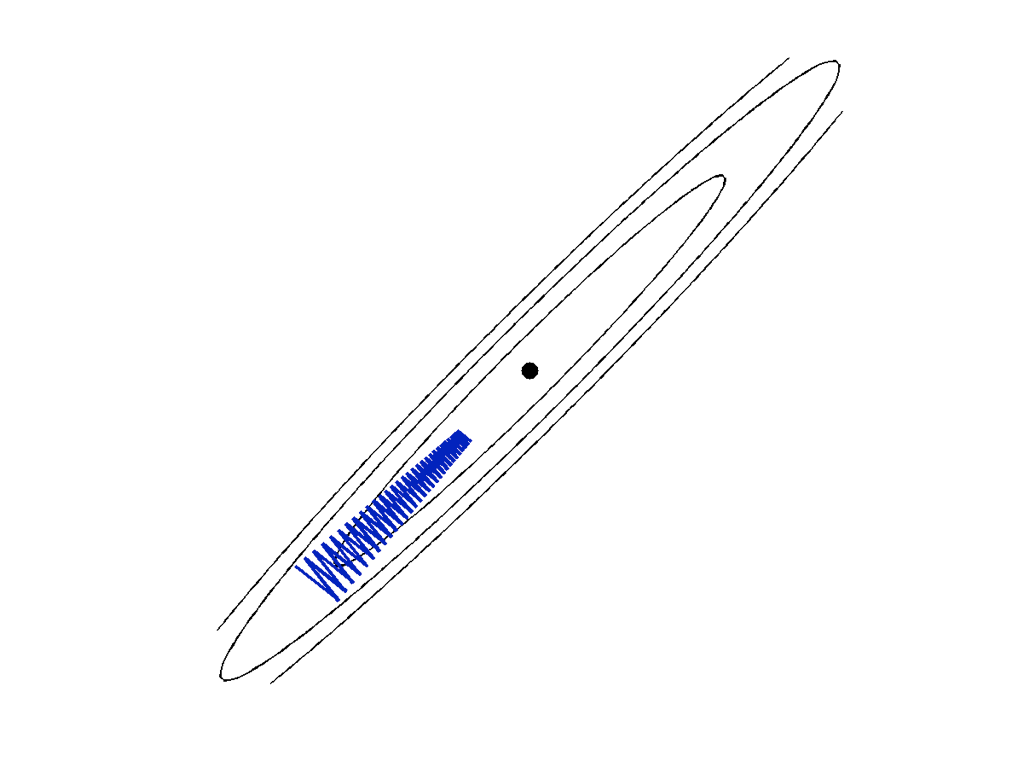
\includegraphics[width=0.4\textwidth,height=\textheight]{assets/gd_osc.png}
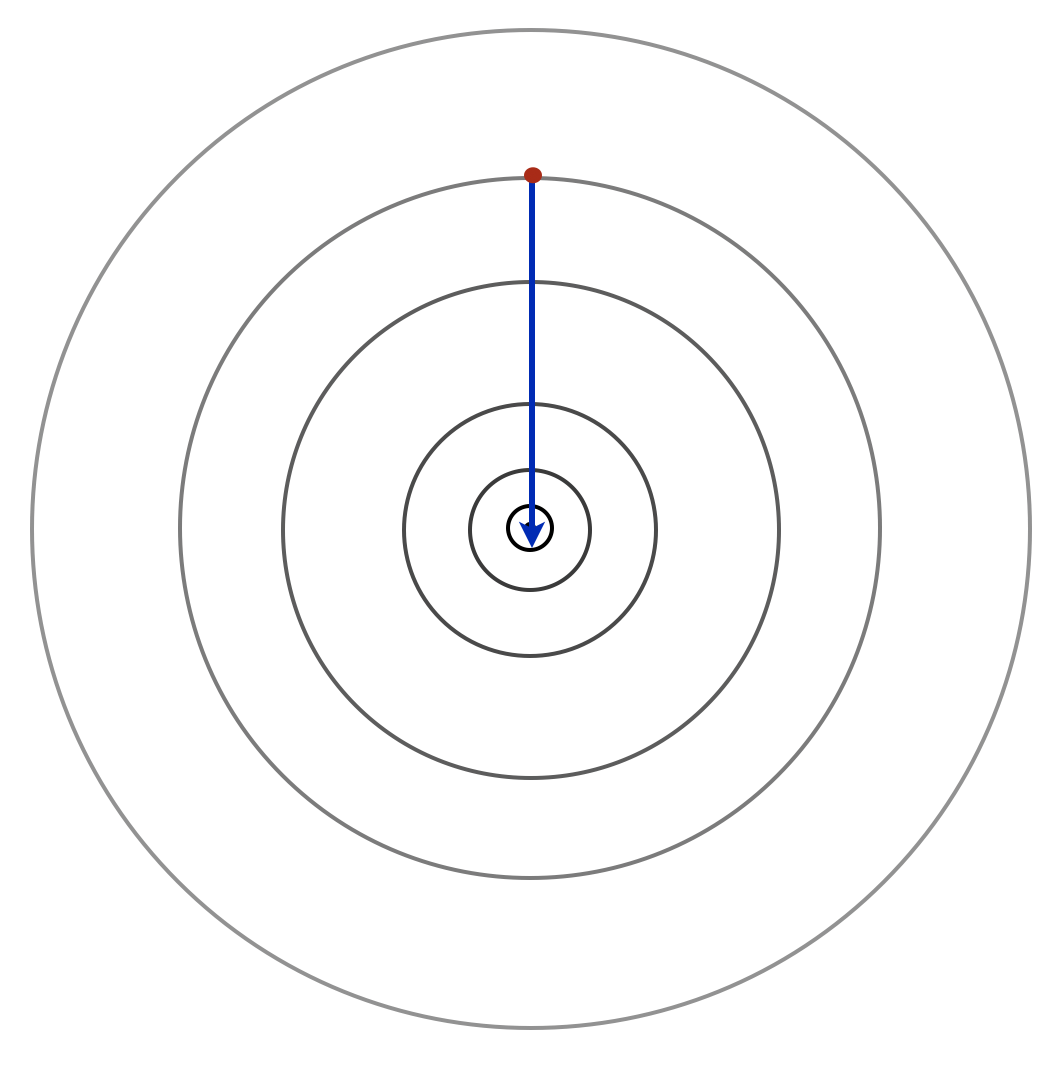
\includegraphics[width=0.3\textwidth,height=\textheight]{assets/gd_nice_condition.png}

There is one final case that's worth considering. When all of the
eigenvalues of~\(Q\) are nonnegative but some of them are zero, the
function~\(\Phi\) is convex but not strongly convex. In this case,
exponential convergence to a unique point cannot be guaranteed. In
particular, there will be an infinite number of global minimizers of
\(\Phi\). If~\(w_\star\) is a global minimizer and~\(v\) is any vector
with \(Qv=0\), then~\(w_\star+v\) is also a global minimizer. However,
in the span of the eigenvectors corresponding to positive eigenvalues,
gradient descent still converges exponentially. For general convex
functions, it will be important to consider different parts of the
parameter space to fully understand the dynamics of gradient methods.

\hypertarget{stochastic-gradient-descent}{%
\section{Stochastic gradient
descent}\label{stochastic-gradient-descent}}

The stochastic gradient method is one of the most popular algorithms for
contemporary data analysis and machine learning. It has a long history
and has been ``invented'' several times by many different communities
(under the names ``least mean squares,'' ``backpropagation,'' ``online
learning,'' and the ``randomized Kaczmarz method''). Most researchers
attribute this algorithm to the initial work of Robbins and Monro from
1951 who solved a more general problem with the same method.\footnote{Robbins
  and Monro, {``A Stochastic Approximation Method,''} \emph{The Annals
  of Mathematical Statistics}, 1951, 400--407.}

Consider again our main goal of minimizing the empirical risk with
respect to a vector of parameters~\(w\), and consider the simple case of
linear classification where~\(w\) is~\(d\)-dimensional and \[
f(x_i;w) = w^Tx_i\,.
\]

The idea behind the stochastic gradient method is that since the
gradient of a sum is the sum of the gradients of the summands, each
summand provides useful information about how to optimize the total sum.
Stochastic gradient descent minimizes empirical risk by following the
gradient of the risk evaluated on a \emph{single, random} example.

\begin{Algorithm}

\textbf{Stochastic Gradient Descent}

\begin{itemize}
\tightlist
\item
  Start from an initial point \(w_0 \in \mathbb{R}^d\).
\item
  At each step \(t=0,1,2,\dots\):

  \begin{itemize}
  \tightlist
  \item
    Choose a step size \(\alpha_t>0\) and random index \(i \in [n]\).
  \item
    Set
    \(w_{t+1} = w_t - \alpha_t \nabla_w \mathit{loss}(f(x_i;w_t),y_i)\)
  \end{itemize}
\end{itemize}

\end{Algorithm}

The intuition behind this method is that by following a descent
direction in expectation, we should be able to get close to the optimal
solution if we wait long enough. However, it's not quite that simple.
Note that even when the gradient of the sum is zero, the gradients of
the individual summands may not be. The fact that~\(w_\star\) is no
longer a fixed point complicates the analysis of the method.

\hypertarget{example-revisiting-the-perceptron}{%
\subsection{Example: Revisiting the
Perceptron}\label{example-revisiting-the-perceptron}}

Let's apply the stochastic gradient method to the support vector machine
cost loss. We initialize our half-space at some~\(w_{0}\). At iteration
\(t\), we choose a random data point~\((x_{i},y_{i})\) and update \[
w_{t+1}= w_{t}+\eta\begin{cases}
y_{i}x_{i} &\text{if}~y_{i}w_{t}^{T}x_{i}\leq 1\\
0 & \text{otherwise}
\end{cases}
\] As we promised earlier, we see that using stochastic gradient descent
to minimize empirical risk with a hinge loss is completely equivalent to
Rosenblatt's Perceptron algorithm.

\hypertarget{example-computing-a-mean}{%
\subsection{Example: Computing a mean}\label{example-computing-a-mean}}

Let's now try to examine the simplest example possible. Consider
applying the stochastic gradient method to the function \[
    \frac{1}{2n} \sum_{i=1}^n  (w-y_i)^2
\] where~\(y_1,\dots,y_n\) are fixed scalars. This setup corresponds to
a rather simple classification problem where the~\(x\) features are all
equal to~\(1\). Note that the gradient of one of the increments is \[
    \nabla \mathit{loss} (f(x_i;w),y) = w-y_i\,.
\]

To simplify notation, let's imagine that our random samples are coming
to us in order~\(\{1,2,3,4,...\}\) Start with~\(w_1=0\), use the step
size \(\alpha_k = 1/k\). We can then observe that \[
\begin{aligned}
w_{2} & =  w_{1}-w_{1}+y_{1}=y_{1}\\
w_{3} & =  w_{2}-\frac{1}{2}\left(w_{2}-y_{2}\right)=\frac{1}{2}y_{1}+\frac{1}{2}y_{2}\\
w_{4} & =   w_{3}-\frac{1}{3}\left(w_{3}-y_{3}\right) = \frac{1}{3}y_{1}+\frac{1}{3}y_{2}+\frac{1}{3}y_{3}
\end{aligned}
\] Thus, we can quickly conclude by induction that \[
w_{k+1} =  \left(\frac{k-1}{k}\right)w_{k}+\frac{1}{k}y_{k}=\frac{1}{k}\sum_{i=1}^{k}y_{i}\,.
\] After~\(n\) steps,~\(w_n\) is the mean of the~\(y_i\), and you can
check by taking a gradient that this is indeed the minimizer of the ERM
problem.

The~\(1/k\) step size was the originally proposed step size by Robbins
and Monro. This simple example justifies why: we can think of the
stochastic gradient method as computing a running average. Another
motivation for the~\(1/k\) step size is that the steps tend to zero, but
the path length is infinite.

Moving to a more realistic random setting where the data might arrive in
any order, consider what happens when we run the stochastic gradient
method on the function \[
    R(w) = \tfrac{1}{2} \mathbb{E}[ (w-Y)^2]\,.
\] Here~\(Y\) is some random variable with mean~\(\mu\) and variance
\(\sigma^2\). If we run for~\(k\) steps with i.i.d. samples~\(Y_i\) at
each iteration, the calculation above reveals that \[
    w_k = \frac{1}{k} \sum_{i=1}^k Y_i\,.
\] The associated cost is \[
    R(w_k) = \frac{1}{2} \mathop\mathbb{E}\left[ \left(\frac{1}{k} \sum_{i=1}^k Y_i-Y\right)^2\right]
    = \frac{1}{2k}\sigma^2 + \frac{1}{2}\sigma^2\,.
\] Compare this with the cost of the exact minimizer~\(w_\star\) of
\(R(w)\). Expanding the definition \[
    R(w) = \tfrac{1}{2} \mathbb{E}[w^2 - 2 Y w + Y^2] = \tfrac{1}{2}w^2 - 2 \mu Y + \tfrac{1}{2}\sigma^2 + \tfrac{1}{2}\mu^2\,,
\] we find that the minimizer is~\(w_\star=\mu\). Its cost is \[
    R(w_\star) = \frac{1}{2} \sigma^2\,,
\] and after~\(n\) iterations, we have the \emph{optimality gap} \[
    R(w)-R(w_\star) = \frac{1}{2n}\sigma^2\,.
\] This is the best we could have achieved using any estimator for
\(w_\star\) given the collection of random draws. Interestingly, the
incremental ``one-at-a-time'' method finds as good a solution as one
that considers all of the data together. This basic example reveals a
fundamental limitation of the stochastic gradient method: we can't
expect to generically get fast convergence rates without additional
assumptions. Statistical fluctuations themselves prevent the optimality
gap from decreasing exponentially quickly.

This simple example also helps give intuition on the convergence as we
sample stochastic gradients. The figure below plots an example of each
individual term in the summand, shaded with colors of blue to
distinguish each term. The minimizing solution is marked with a red
star. To the far left and far right of the figure, all of the summands
will have gradients pointing in the same direction to the solution.
However, as our iterate gets close to the optimum, we will be pointed in
different directions depending on which gradient we sample. By reducing
the step size, we will be more likely to stay close and eventually
converge to the optimal solution.

\begin{figure}
\centering
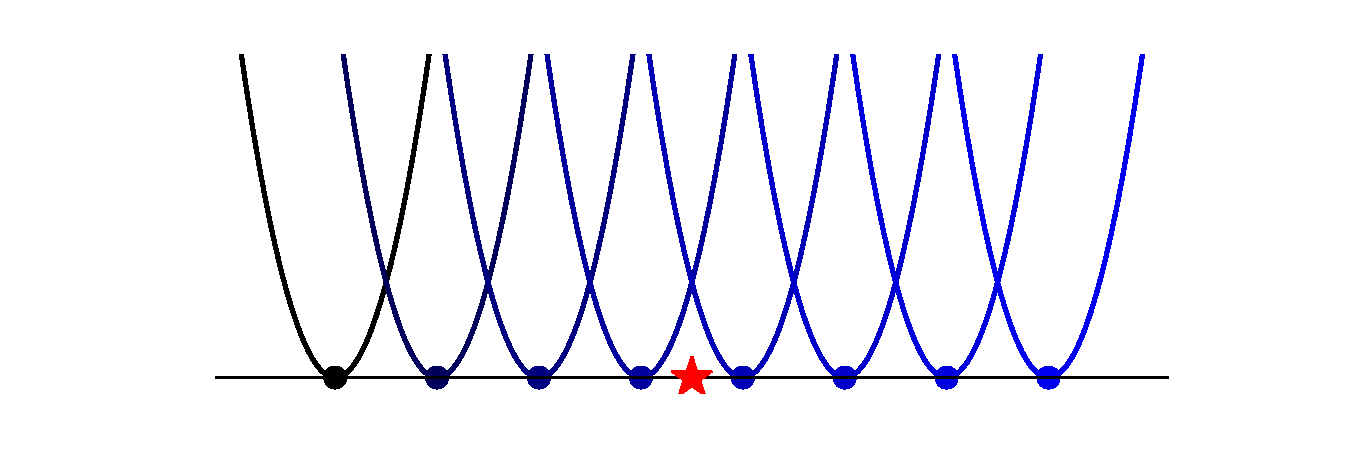
\includegraphics{assets/confusion_region}
\caption{Plot of the different increments of
\(\tfrac{1}{2n} \sum_{i=1}^n (w-y_i)^2\). The red star denotes the
optimal solution.}
\end{figure}

\hypertarget{example-stochastic-minimization-of-a-quadratic-function}{%
\subsection{Example: stochastic minimization of a quadratic
function}\label{example-stochastic-minimization-of-a-quadratic-function}}

Let's consider a more general version of stochastic gradient descent
that follows the gradient plus some unbiased noise. We can model the
algorithm as minimizing a function~\(\Phi(w)\) where we follow a
direction \(\nabla \Phi(w) + \nu\) where~\(\nu\) is a random vector with
mean zero and \(\mathop\mathbb{E}[\Vert \nu \Vert^2] = \sigma^2\).
Consider the special case where \(\Phi(w)\) is a quadratic function \[
    \Phi(w) = \tfrac{1}{2} w^T Q w - p^T w +r\,.
\] Then the iterations take the form \[
    w_{t+1} = w_t - \alpha (  Qw_t -p  + \nu_t)\,.
\] Let's consider what happens when~\(Q\) is positive definite with
maximum eigenvalue~\(\lambda_1\) and minimum
eigenvalue~\(\lambda_d >0\). Then, if~\(w_\star\) is a global minimizer
of~\(Q\), we can again rewrite the iterations as \[
    w_{t+1}-w_\star = (I-\alpha Q) (w_t-w_\star) - \alpha\nu_t\,.
\] Since we assume that the noise~\(\nu_t\) is independent of all of the
\(w_k\) with~\(k \leq t\), we have \[
    \mathop\mathbb{E}[ \Vert w_{t+1}-w_\star \Vert^2 ]= \Vert I-\alpha Q \Vert^2 \mathop\mathbb{E}[ \Vert w_t-w_\star\Vert^2 ] + \alpha^2\sigma^2\,.
\] which looks like the formula we derived for quadratic functions, but
now with an additional term from the noise. Assuming
\(\alpha < 1/\lambda_1\), we can unwind this recursion to find \[
    \mathop\mathbb{E}[ \Vert w_{t}-w_\star \Vert^2 ]\leq ( 1-\alpha \lambda_d)^{2t} \Vert w_0-w_\star\Vert^2  + \frac{\alpha \sigma^2}{\lambda_d}\,.
\] From this expression, we see that gradient descent converges
exponentially quickly to some ball around the optimal solution. The
smaller we make~\(\alpha\), the closer we converge to the optimal
solution, but the rate of convergence is also slower for smaller
\(\alpha\). This tradeoff motivates many of the step size selection
rules in stochastic gradient descent. In particular, it is common to
start with a large step size and then successively reduce the step size
as the algorithm progresses.

\hypertarget{tricks-of-the-trade}{%
\subsection{Tricks of the trade}\label{tricks-of-the-trade}}

In this section, we describe key engineering techniques that are useful
for tuning the performance of stochastic gradient descent. Every machine
learning practitioner should know these simple tricks.

\textbf{Shuffling.} Even though we described the stochastic gradient
method a sampling each gradient with replacement from the increments, in
practice better results are achieved by simply randomly permuting the
data points and then running SGD in this random order. This is called
``shuffling,'' and even a single shuffle can eliminate the pathological
behavior we described in the example with highly correlated data.
Recently, beginning with work by Gürbüzbalaban et al., researchers have
shown that in theory, shuffling outperforms independent sampling of
increments.\footnote{Gürbüzbalaban, Ozdaglar, and Parrilo, {``Why Random
  Reshuffling Beats Stochastic Gradient Descent,''} \emph{Mathematical
  Programming}, 2019, 1--36.} The arguments for without-replacement
sampling remain more complicated than the with-replacement derivations,
but optimal sampling for SGD remains an active area of optimization
research.

\textbf{Step size selection.} Step size selection in SGD remains a hotly
debated topic. We saw above a decreasing stepsize~\(1/k\) solved our
simple one dimensional ERM problem. However, a rule that works for an
unreasonable number of cases is to simply pick the largest step size
which does not result in divergence. This step will result in a model
that is not necessarily optimal, but significantly better than
initialization. By slowly reducing the step size from this initial large
step size to successively smaller ones, we can zero in on the optimal
solution.

\textbf{Step decay.} The step size is usually reduced after a fixed
number of passes over the training data. A pass over the entire data set
is called an \emph{epoch}. In an epoch, some number of iterations are
run, and then a choice is made about whether to change the step size. A
common strategy is to run with a constant step size for some fixed
number of iterations \(T\), and then reduce the step size by a constant
factor~\(\gamma\). Thus, if our initial step size is~\(\alpha\), on
the~\(k\)th epoch, the step size is~\(\alpha \gamma^{k-1}\). This method
is often more robust in practice than the diminishing step size rule.
For this step size rule, a reasonable heuristic is to choose~\(\gamma\)
between~\(0.8\) and~\(0.9\). Sometimes people choose rules as aggressive
as~\(\gamma = 0.1\).

Another possible schedule for the step-size is called \emph{epoch
doubling}. In epoch doubling, we run for~\(T\) steps with step
size~\(\alpha\), then run~\(2T\) steps with step size~\(\alpha/2\), and
then~\(4T\) steps with step size~\(\alpha/4\) and so on. Note that this
provides a piecewise constant approximation to the
function~\(\alpha/k\).

\textbf{Minibatching.} A common technique used to take advantage of
parallelism is called \emph{minibatching}. A minibatch is an average of
many stochastic gradients. Suppose at each iteration we sample a
\(\mathrm{batch}_k\) with~\(m\) data points. The update rule then
becomes \[
    w_{k+1} = w_{k} -\alpha_k  \frac{1}{m}\sum_{j\in \mathrm{batch}_k} \nabla_w  \mathit{loss}(f(x_j;w_k),y_j)\,.
\] Minibatching reduces the variance of the stochastic gradient estimate
of the true gradient, and hence tends to be a better descent direction.
Of course, there are tradeoffs in total computation time versus the size
of the minibatch, and these typically need to be handled on a case by
case basis.

\textbf{Momentum.} Finally, we note that one can run stochastic gradient
descent with \emph{momentum}. Momentum mixes the current gradient
direction with the previously taken step. The idea here is that if the
previous weight update was good, we may want to continue moving along
this direction. The algorithm iterates are defined as \[
w_{k+1}=w_{k}-\alpha_{k}g_k\left(w_{k}\right) + \beta (w_{k}+w_{k-1})\,,
\] where~\(g_k\) denotes a stochastic gradient. In practice, these
methods are very successful. Typical choices for~\(\beta\) here are
between~\(0.8\) and~\(0.95\). Momentum can provide significant
accelerations, and should be considered an option in any implementation
of SGM.

\textbf{The SGD Quick Start Guide.} Newcomers to stochastic gradient
descent often find all of these design choices daunting, and it's useful
to have simple rules of thumb to get going. We recommend the following:

\begin{enumerate}
\def\labelenumi{\arabic{enumi}.}
\tightlist
\item
  Pick as large a minibatch size as you can given your computer's RAM.
\item
  Set your momentum parameter to either 0 or 0.9. Your call!
\item
  Find the largest constant stepsize such that SGD doesn't diverge. This
  takes some trial and error, but you only need to be accurate to within
  a factor of 10 here.
\item
  Run SGD with this constant stepsize until the empirical risk plateaus.
\item
  Reduce the stepsize by a constant factor (say, 10)
\item
  Repeat steps 4 and 5 until you converge.
\end{enumerate}

While this approach may not be the most optimal in all cases, it's a
great starting point and is good enough for probably 90\% of
applications we've encountered.

\hypertarget{analysis-of-the-stochastic-gradient-method}{%
\section{Analysis of the stochastic gradient
method}\label{analysis-of-the-stochastic-gradient-method}}

We now turn to a theoretical analysis of the general stochastic gradient
method. Before we proceed, let's set up some conventions. We will assume
that we are trying to minimize a convex function
\(R:\mathbb{R}^d \rightarrow \mathbb{R}\). Let~\(w_\star\) denote any
optimal solution of~\(R\). We will assume we gain access at every
iteration to a \emph{stochastic function} \(g(w;\xi)\) such that \[
    \mathbb{E}_\xi[g(w; \xi)] = \nabla R(w)\,.
\] Here~\(\xi\) is a random variable which determines what our direction
looks like. We additionally assume that these stochastic gradients are
\emph{bounded} so there exists a non-negative constants~\(B\) such that
\[
     \Vert g(w;\xi)\Vert \leq  B\,.
\]

We will study the stochastic gradient iteration \[
w_{t+1}=w_{t}-\alpha_{t}g\left(w_{t};\xi_t\right)\,.
\] Throughout, we will assume that the sequence~\(\{\xi_j\}\) is
selected i.i.d. from some fixed distribution.

We begin by expanding the distance to the optimal solution \[
\begin{aligned}
 \Vert w_{t+1} - w_\star \Vert^2 &=
 \Vert  w_t - \alpha_t g_t(w_t;\xi_t) - w_\star \Vert^2  \\
 &= \Vert w_t - w_\star\Vert^2 -2 \alpha_t \langle g_t( w_t;\xi_t), w_t- w_\star \rangle + \alpha_t^2 \Vert g_t(w_t; \xi_t) \Vert^2
\end{aligned}
\]

We deal with each term in this expansion separately. First note that if
we apply the law of iterated expectation \[
\begin{aligned}
    \mathbb{E}[ \langle g_t(w_t;\xi_t), w_t - w_\star \rangle ]
    &= \mathbb{E}\left[\mathbb{E}_{\xi_t}[  \langle g_t(w_t;\xi_t), w_t - w_\star \rangle \mid  \xi_0,\ldots,\xi_{t-1} ]\right]\\
    &= \mathbb{E}\left[  \langle\mathbb{E}_{\xi_t}[  g_t(w_t;\xi_t)  \mid  \xi_0,\ldots,\xi_{t-1} ] , w_t - w_\star \rangle\right]\\
    &= \mathbb{E}\left[ \langle \nabla R(w_t) , w_t - w_\star \rangle\right]\,.
\end{aligned}
\] Here, we are simply using the fact that~\(\xi_t\) being independent
of all of the preceding~\(\xi_i\) implies that it is independent
of~\(w_t\). This means that when we iterate the expectation, the
stochastic gradient can be replaced by the gradient.

The last term we can bound using our assumption that the gradients are
bounded \[
\begin{aligned}
\mathbb{E}[ \Vert g(w_t; \xi_t)\Vert^2]  \leq B^2
\end{aligned}
\]

Letting~\(\delta_t := \mathbb{E}[\Vert w_{t}-w_\star\Vert^2]\), this
gives \[
 \delta_{t+1} \leq \delta_t - 2 \alpha_t \mathbb{E}\left[ \langle \nabla R(w_t) , w_t - w_\star \rangle\right] + \alpha_t^2 B^2\,.
\]

Now let~\(\lambda_t = \sum_{j=0}^t \alpha_j\) denote the sum of all the
step sizes up to iteration~\(t\). Also define the average of the
iterates weighted by the step size \[
    \bar{w}_t = \lambda_t^{-1} \sum_{j=0}^t \alpha_j w_j\,.
\] We are going to analyze the deviation of~\(R(\bar{w}_t)\) from
optimality.

Also let~\(\rho_0 = \Vert w_0-w_\star\Vert^2\).~\(\rho_0\) is the
initial distance to an optimal solution. It is not necessarily a random
variable.

To proceed, we just expand the following expression: \[
\begin{aligned}
\mathbb{E}\left[  R\left (\bar{w}_T \right)  - R(w_\star)  \right]  & \leq
    \mathbb{E}\left[ \lambda_T^{-1} \sum_{t=0}^T \alpha_t( R(w_t)  - R(w_\star) ) \right] \\
    &\leq   \lambda_T^{-1} \sum_{t=0}^T \alpha_t \mathbb{E}[ \langle \nabla R(x_t), w_t-w_\star \rangle ]\\
    &\leq   \lambda_T^{-1} \sum_{t=0}^T \tfrac{1}{2}(\delta_{t}-\delta_{t+1})+ \tfrac{1}{2} \alpha_t^2 B^2\\
    & = \frac{\delta_0 - \delta_{T+1} +  B^2 \sum_{t=0}^T \alpha_t^2}{2 \lambda_T}\\
    & \leq \frac{\rho_0^2  + B^2 \sum_{t=0}^T \alpha_t^2}{2 \sum_{t=0}^T \alpha_t}
\end{aligned}
\] Here, the first inequality follows because~\(R\) is convex (the line
segments lie above the function, i.e.,
\(R(w_\star) \geq R(w_t) + \langle\nabla R(w_t), w_t-w_\star\rangle\)).
The second inequality uses the fact that gradients define tangent planes
to~\(R\) and always lie below the graph of~\(R\), and the third
inequality uses the recursion we derived above for~\(\delta_t\).

With this in hand, we can now prove the following result.\footnote{Nemirovski
  et al., {``Robust Stochastic Approximation Approach to Stochastic
  Programming,''} \emph{SIAM Journal on Optimization} 19, no. 4 (2009):
  1574--1609.}

\begin{Theorem}

Suppose we run the SGM on a convex~\(R\) for~\(T\) steps with step size
\(\alpha\). Define \[
    \alpha_{\mathrm{opt}} = \frac{\rho_0}{B\sqrt{T}}
\] and~\(\theta = \alpha/\alpha_{\mathrm{opt}}.\) Then, we have the
bound \[
\mathbb{E}[R(\bar{w}_T) - R_\star] \leq \left(\tfrac{1}{2} \theta + \tfrac{1}{2} \theta^{-1}\right) \frac{B \rho_0}{\sqrt{T}}  \,.
\]

\end{Theorem}

This proposition asserts that we pay linearly for errors in selecting
the optimal constant step size. If we guess a constant step size that is
two-times or one-half of the optimal choice, then we need to run for
twice as many iterations. The optimal step-size is found by minimizing
our upper bound on the suboptimality gap. Other step sizes could also be
selected here, including diminishing step size. But the constant step
size turns out to be optimal for this upper bound.

What are the consequences for risk minimization? First, for
\emph{empirical risk}, assume we are minimizing a convex loss function
and searching for a linear predictor. Assume further that there exists a
model with zero empirical risk. Let~\(C\) be the maximum value of the
gradient of the loss function,~\(D\) be the largest norm of any
example~\(x_i\) and let~\(\rho\) denote the minimum norm~\(w\) such
that~\(R_S[w]=0\). Then we have \[
\mathbb{E}[R_S[\bar{w}_T]] \leq \frac{CD\rho}{\sqrt{T}}  \,.
\] we see that with appropriately chosen step size, the stochastic
gradient method converges at a rate of~\(1/\sqrt{T}\), the same rate of
convergence observed when studying the one-dimensional mean computation
problem. Again, the stochasticity forces us into a slow,~\(1/\sqrt{T}\)
rate of convergence, but high dimensionality does not change this rate.

Second, if we only operate on samples exactly once, and we assume our
data is i.i.d., we can think of the stochastic gradient method as
minimizing the \emph{population risk} instead of the empirical risk.
With the same notation, we'll have \[
\mathbb{E}[R[\bar{w}_T]] -R_\star \leq \frac{CD\rho}{\sqrt{T}}  \,.
\] The analysis of stochastic gradient gives our second
\emph{generalization bound} of the book. What it shows is that by
optimizing over a fixed set of~\(T\) data points, we can get a solution
that will have low cost on new data. We will return to this observation
in the next chapter.

\hypertarget{implicit-convexity}{%
\section{Implicit convexity}\label{implicit-convexity}}

\index{convexity!implicit}

We have thus far focused on convex optimization problems, showing that
gradient descent can find global minima with modest computational means.
What about nonconvex problems? Nonconvex optimization is such a general
class of problems that in general it is hard to make useful guarantees.
However, ERM is a special optimization problem, and its structure
enables nonconvexity to enter in a graceful way.

As it turns out there's a ``hidden convexity'' of ERM problems which
shows that the \emph{predictions} should converge to a global optimum
even if we can't analyze to where exactly the model converges. We will
show this insight has useful benefits when models are overparameterized
or nonconvex.

Suppose we have a loss function~\(\mathit{loss}\) that is equal to zero
when \(\hat{y} = y\) and is nonnegative otherwise. Suppose we have a
generally parameterized function class~\(f(x;w)\) and we aim to find the
best~\(w\) to minimize the empirical risk. The empirical risk \[
R_S[w] =\frac{1}{n} \sum_{i=1}^n \mathit{loss}(f(x_i;w),y_i)\,.
\] is bounded below by~\(0\). Hence if we can find a solution with
\(f(x_i;w)=y_i\) for all~\(i\), we would have a \emph{global minimum}
not a local minimum. This is a trivial observation, but one that helps
focus our study: if we can show~\(f(x_i;w)\) converges to~\(y_i\) for
all~\(i\), we will have computed a global minimizer.

For the sake of simplicity, we specialize to the square loss in this
section: \[
 \mathit{loss}(f(x_i;w),y_i) =  \tfrac{1}{2} (f(x_i;w)-y_i)^2\,.
\] The argument we develop here is inspired by the work of Du \emph{et
al.} who use a similar approach to rigorously analyze the convergence of
two layer neural networks.\footnote{Du et al., {``Gradient Descent
  Provably Optimizes over-Parameterized Neural Networks,''} in
  \emph{International Conference on Learning Representations}, 2019.}
Similar calculations can be made for other losses with some
modifications of the argument.

\hypertarget{convergence-of-overparameterized-linear-models}{%
\subsection{Convergence of overparameterized linear
models}\label{convergence-of-overparameterized-linear-models}}

Let's first consider the case of linear prediction functions \[
    f(x;w) = w^T x\,.
\] Define \[
    y = \begin{bmatrix}
        y_1\\ \vdots \\ y_n
    \end{bmatrix}\qquad \qquad \text{and}\qquad \qquad X = \begin{bmatrix} x_1^T \\ \vdots \\x_n^T \end{bmatrix}\,.
\] We can then write the empirical risk objective as \[
R_S[w]=\frac1{2n}\|Xw-y\|^2\,.
\] The gradient descent update rule has the form\marginnote{We pull the
scaling factor~\(1/n\) into the step size for notational convenience.}
\[
    w_{t+1} = w_t - \alpha X^T (X w_t-y)\,.
\] Now define the vector of predictions \[
\hat{y}_t = \begin{bmatrix}
        f(x_1;w_t) \\ \vdots \\ f(x_n;w_t)
    \end{bmatrix}\,.
\] For the linear case, the predictions are given by
\(\hat{y}_k = X w_k\). We can use this definition to track the evolution
of the \emph{predictions} instead of the parameters~\(w\). The
predictions evolve according to the rule \[
    \hat{y}_{t+1} = \hat{y}_t - \alpha X X^T (\hat{y}_t-y)\,.
\] This looks a lot like the gradient descent algorithm applied to a
strongly convex quadratic function that we studied earlier. Subtracting
\(y\) from both sides and rearranging shows \[
    \hat{y}_{t+1}-y = (I - \alpha X X^T) (\hat{y}_t-y)\,.
\] This expression proves\marginnote{Keep in mind that~\(X\)
is~\(n\times d\) and a model is overparameterized if~\(d>n\).
The~\(n\times n\) matrix~\(XX^T\) has a chance of being strictly
positive definite in this case.} that as long as~\(XX^T\) is strictly
positive definite and~\(\alpha\) is small enough, then the predictions
converge to the training labels. When we use a sufficiently small and
constant step size~\(\alpha\), our predictions converge at an
\emph{exponential} rate. This is in contrast to the behavior we saw for
gradient methods on overdetermined problems. Our general analysis of the
weights showed that the convergence rate might be only inverse
polynomial in the iteration counter. In the overparameterized regime, we
can guarantee the predictions converge more rapidly than the weights
themselves.

The rate in this case is governed by properties of the matrix~\(X\). As
we have discussed we need the eigenvalues of~\(XX^T\) to be positive,
and we'd ideally like that the eigenvalues are all of similar magnitude.

First note that a \emph{necessary} condition is that~\(d\), the
dimension, must be larger than~\(n\), the number of data points. That
is, we need to have an overparameterized model in order to ensure
exponentially fast convergence of the predictions. We have already seen
that such overparameterized models make it possible to interpolate any
set of labels and to always force the data to be linearly separable.
Here, we see further that overparameterization encourages optimization
methods to converge in fewer iterations by improving the condition
number of the data matrix.

Overparameterization can also help accelerate convergence. Recall that
the eigenvalues of~\(XX^T\) are the squares of the \emph{singular
values} of \(X\). Let us write out a singular value decomposition
for~\(X\): \[
    X = USV^T
\] where~\(S\) is a diagonal matrix of singular values
\((\sigma_1,\ldots, \sigma_n)\). In order to improve the condition
number of this matrix, it suffices to add a feature that is concentrated
in the span of the singular vectors with small singular values. How to
find such features is not always apparent, but does give us a starting
point as to where to look for new, informative features.

\hypertarget{convergence-of-nonconvex-models}{%
\subsection{Convergence of nonconvex
models}\label{convergence-of-nonconvex-models}}

\index{nonconvex}

Surprisingly, this analysis naturally extends to nonconvex models. With
some abuse of notation, let~\(\hat y = f(x;w)\in\mathbb{R}^n\) denote
the~\(n\) predictions of some nonlinear model parameterized by the
weights~\(w\) on input~\(x\). Our goal is to minimize the squared loss
objective \[
\frac12\|f(x;w)-y\|^2\,.
\] Since the model is nonlinear this objective is no longer convex.
Nonetheless we can mimic the analysis we did previously for
overparameterized linear models.

Running gradient descent on the weights gives \[
    w_{t+1}
    = w_t - \alpha \mathsf{D} f (x;w_t)(\hat{y}_t - y)\,,
\] where~\(\hat y_t=f(x;w_t)\) and~\(\mathsf{D} f\) is the Jacobian of
the predictions with respect to~\(w\). That is,~\(\mathsf{D} f (x;w)\)
is the \(d\times n\) matrix of first order derivatives of the
function~\(f(x;w)\) with respect to~\(w\). We can similarly define the
Hessian operator~\(H(w)\) to be the~\(n \times d \times d\) array of
second derivatives of~\(f(x;w)\). We can think of~\(H(w)\) as a
quadratic form that maps pairs of vectors
\((u,v) \in \mathbb{R}^{d\times d}\) to~\(\mathbb{R}^n\). With these
higher order derivatives, Taylor's theorem asserts \[
\begin{aligned}
    \hat{y}_{t+1} &= f(x,w_{t+1})\\
    &= f(x,w_t) +  \mathsf{D} f (x;w_t)^T(w_{t+1}-w_t) \\
    &\qquad\qquad+  \int_0^1 H(w_t+s (w_{t+1}-w_t))  (w_{t+1}-w_t, w_{t+1}-w_t) \mathrm{d} s\,.
\end{aligned}
\] Since~\(w_t\) are the iterates of gradient descent, this means that
we can write the prediction as \[
\begin{aligned}
    \hat{y}_{t+1}   &= \hat{y}_t -\alpha \mathsf{D} f(x;w_t)^T \mathsf{D} f(x;w_t)(\hat{y_t} - y)
            + \alpha \epsilon_t \,,
\end{aligned}
\] where \[
\epsilon_t = \alpha \int_0^1 H(w_t+s (w_{t+1}-w_t))
    \left( \mathsf{D} f(x;w_t) (\hat{y}_t - y),\mathsf{D} f(x;w_t) (\hat{y}_t - y)\right)\mathrm{d} s\,.
\] Subtracting the labels~\(y\) from both sides and rearranging terms
gives the recursion \[
    \hat{y}_{t+1}-y = (I -  \alpha \mathsf{D} f(x;w_t)^T \mathsf{D} f(x;w_t))(\hat{y}_t - y) + \alpha \epsilon_t\,.
\] If~\(\epsilon_t\) vanishes, this shows that the predictions again
converge to the training labels as long as the eigenvalues of
\(\mathsf{D} f(x;w_t)^T \mathsf{D} f(x;w_t)\) are strictly positive.
When the error vector~\(\epsilon_t\) is sufficiently small, similar
dynamics will occur. We expect~\(\epsilon_t\) to not be too large
because it is quadratic in the distance of~\(y_t\) to~\(y\) and because
it is multiplied by the stepsize~\(\alpha\) which can be chosen to be
small.

The nonconvexity isn't particularly disruptive here. We just need to
make sure our Jacobians have full rank most of the time and that our
steps aren't too large. Again, if the number of parameters are larger
than the number of data points, then these Jacobians are likely to be
positive definite as long as we've engineered them well. But how exactly
can we guarantee that our Jacobians are well behaved? We can derive some
reasonable ground rules by unpacking how we compute gradients of
compositions of functions. More on this follows in our chapter on deep
learning.

\hypertarget{regularization}{%
\section{Regularization}\label{regularization}}

\index{regularization}

The topic of \emph{regularization} belongs somewhere between
optimization and generalization and it's one way of connecting the two.
Hence, we will encounter it in both chapters. Indeed, one complication
with optimization in the overparameterized regime is that there is an
\emph{infinite collection} of models that achieve zero empirical risk.
How do we break ties between these and which set of weights should we
prefer?

To answer this question we need to take a step back and remember that
the goal of supervised learning is not just to achieve zero training
error. We also care about performance on data \emph{outside} the
training set, and having zero loss on its own doesn't tell us anything
about data outside the training set.

As a toy example, imagine we have two sets of
data~\(X_{\mathrm{train}}\) and~\(X_{\mathrm{test}}\)
where~\(X_{\mathrm{train}}\) has shape \(n \times d\)
and~\(X_{\mathrm{test}}\) is~\(m \times d\). Let \(y_{\mathrm{train}}\)
be the training labels and let~\(q\) be an \(m\)-dimensional vector of
random labels. Then if~\(d>(m+n)\) we can find weights~\(w\) such that
\[
    \begin{bmatrix}
     X_{\mathrm{train}} \\ X_{\mathrm{test}}
    \end{bmatrix} w =
    \begin{bmatrix}
     y_{\mathrm{train}} \\ q
    \end{bmatrix}
\] That is, these weights would produce zero error on the training set,
but error no better than random guessing on the testing set. That's not
desired behavior! Of course this example is pathological, because in
reality we would have no reason to fit random labels against the test
set when we create our model.

The main challenge in supervised learning is to design models that
achieve low training error while performing well on new data. The main
tool used in such problems is called \emph{regularization}.
Regularization is the general term for taking a problem with infinitely
many solutions and biasing its solution towards a smaller subset of
solution space. This is a highly encompassing notion.

Sometimes regularization is \emph{explicit} insofar as we have a desired
property of the solution in mind which we exercise as a constraint on
our optimization problem. Sometimes regularization is \emph{implicit}
insofar as algorithm design choices lead to a unique solution, although
the properties of this solution might not be immediately
apparent.\index{regularization!implicit}\index{regularization!explicit}

Here, we take an unconventional tack of working from implicit to
explicit, starting with stochastic gradient descent.

\hypertarget{implicit-regularization-by-optimization}{%
\subsection{Implicit regularization by
optimization}\label{implicit-regularization-by-optimization}}

\index{regularization!implicit}

Consider again the linear case of gradient descent or stochastic
gradient descent: \[
    w_{t+1} = w_t - \alpha e_t x_t
\] where~\(e_t\) is the gradient of the loss at the current prediction.
Note that if we initialize~\(w_0=0\), then~\(w_t\) is always in the span
of the data. This can be seen by simple induction. This already shows
that even though general weights lie in a high dimensional, SGD searches
over a space with dimension at most~\(n\), the number of data points.

Now suppose we have a nonnegative loss with
\(\frac{\partial \mathit{loss}(z,y)}{\partial z} = 0\) if and only
if~\(y=z\). This condition is satisfied by the square loss, but not
hinge and logistic losses. For such losses, at optimality we have for
some vector~\(v\) that:

\begin{enumerate}
\def\labelenumi{\arabic{enumi}.}
\tightlist
\item
  \(Xw = y\,,\) because we have zero loss.
\item
  \(w = X^T v\,,\) because we are in the span of the data.
\end{enumerate}

Under the mild assumption that our examples are linearly independent, we
can combine these equations to find that \[
    w=X^T(XX^T)^{-1}y\,.
\] That is, when we run stochastic gradient descent we converge to a
very specific solution. Even though we were searching through an
\(n\)-dimensional space, we converge to a unique point in this space.

This special~\(w\) is the \emph{minimum Euclidean norm solution}
of~\(Xw=y\). In other words, out of all the linear prediction functions
that interpolate the training data, SGD selects the solution with the
minimal Euclidean norm. To see why this solution has minimal norm,
suppose that \(\hat{w} = X^T\alpha + v\) with~\(v\) orthogonal to
all~\(x_i\). Then we have \[
X\hat{w} = XX^T\alpha + Xv = XX^T\alpha \,.
\] Which means~\(\alpha\) is completely determined and hence
\(\hat{w} = X^T(XX^T)^{-1}y+ v\). But now \[
    \Vert \hat{w}\Vert^2 = \Vert X^T(XX^T)^{-1}y\Vert^2 + \Vert v \Vert^2\,.
\] Minimizing the right hand side shows that~\(v\) must equal zero.

We now turn to showing that such minimum norm solutions have important
robustness properties that suggest that they will perform well on new
data. In the next chapter, we will prove that these methods are
guaranteed to perform well on new data under reasonable assumptions.

\hypertarget{margin-and-stability}{%
\subsection{Margin and stability}\label{margin-and-stability}}

\index{margin}\index{stability}

Consider a linear classifier that makes no classification errors and
hence perfectly separates the data. Recall that the \emph{decision
boundary} of this classifier is the
hyperplane~\(\mathcal{B}= \{z\,:\,w^Tz = 0\}\) and the \emph{margin} of
the classifier is the distance of the decision boundary from to data: \[
    \mathrm{margin}(w) = \min_i \operatorname{dist}\left(x_i,\mathcal{B}\right)\,.
\] Since we're assuming that~\(w\) correctly classifies all of the
training data, we can write the margin in the convenient form \[
    \operatorname{margin}(w) = \min_i \frac{y_i w^Tx_i}{\Vert w\Vert}\,.
\]

Ideally, we'd like our data to be far away from the boundary and hence
we would like our classifier to have large margin. The reasoning behind
this desideratum is as follows: If we expect new data to be similar to
the training data and the decision boundary is far away from the
training data, then it would be unlikely for a new data point to lie on
the wrong side of the decision boundary. Note that margin tells us how
large a perturbation in the~\(x_i\) can be handled before a data point
is misclassified. It is a robustness measure that tells us how sensitive
a classifier is to changes in the data itself.

Let's now specialize margin to the interpolation regime described in the
previous section. Under the assumption that we interpolate the labels so
that~\(w^Tx_i=y_i\), we have \[
    \operatorname{margin}(w) = \Vert w\Vert^{-1}
\] If we want to simultaneously maximize margin and interpolate the
data, then the optimal solution is to choose the minimum norm solution
of~\(Xw=y\). This is precisely the solution found by SGD and gradient
descent.

Note that we could have directly tried to maximize margin by solving the
constrained optimization problem \[
\begin{array}{ll}
    \text{minimize} & \Vert w \Vert^2\\
    \text{subject to} & y_i w^Tx_i \geq 1\,.
\end{array}
\] This optimization problem is the classic formulation of the support
vector machine. The support vector machine is an example of
\emph{explicit} regularization. Here we declare exactly which solution
we'd like to choose given that our training error is zero. Explicit
regularization of high dimensional models is as old as machine learning.
In contemporary machine learning, however, we often have to squint to
see how our algorithmic decisions are regularizing. The tradeoff is that
we can run faster algorithms with implicit regularizers. But it's likely
that revisiting classic regularization ideas in the context of
contemporary models will lead to many new insights.

\hypertarget{the-representer-theorem-and-kernel-methods}{%
\subsection{The representer theorem and kernel
methods}\label{the-representer-theorem-and-kernel-methods}}

\index{representer theorem}\index{kernel methods}

As we have discussed so far, it is common in linear methods to restrict
the search space to the span of the data. Even when~\(d\) is large (or
even infinite), this reduces the search problem to one in an
\(n\)-dimensional space. It turns out that under broad generality,
solutions in the span of the data are optimal for most optimization
problems in prediction. Here, we make formal an argument we first
introduced in our discussion of features: for most empirical risk
minimization problems, the optimal model will lie in the span of the
training data.

Consider the \emph{penalized} ERM problem \[
    \text{minimize} \frac{1}{n} \sum_{i=1}^n \mathit{loss}(w^T x_i, y_i) + \lambda \Vert w\Vert^2
\] Here~\(\lambda\) is called a \emph{regularization parameter}. When
\(\lambda=0\), there are an infinite number of~\(w\) that minimize the
ERM problem. But for any~\(\lambda>0\), there is a unique minimizer. The
term regularization refers to adding some prior information to an
optimization problem to make the optimal solution unique. In this case,
the prior information is explicitly encoding that we should prefer~\(w\)
with smaller norms if possible. As we discussed in our chapter on
features, smaller norms tend to correspond to simpler solutions in many
feature spaces. Moreover, we just described that minimum norm solutions
themselves could be of interest in machine learning. A regularization
parameter allows us to explicitly tune the norm of the optimal solution.

For our penalized ERM problem, using the same argument as above, we can
write any~\(w\) as \[
    w = X^T \beta + v
\] for some vectors~\(\beta\) and~\(v\) with~\(v^Tx_i=0\) for all~\(i\).
Plugging this ansatz into the penalized ERM problem yields \[
    \text{minimize}_{\beta,v} \frac{1}{n} \sum_{i=1}^n \mathit{loss}(\beta^T X x_i,y_i) + \lambda \Vert X^T \beta \Vert^2 + \lambda \Vert v\Vert^2\,.
\] Now we can minimize with respect to~\(v\), seeing that the only
option is to set~\(v=0\). Hence, we must have that the optimum model
lies in the span of the data: \[
    w = X^T \beta \,.
\] This derivation is commonly called the \emph{representer theorem} in
machine learning. As long as the cost function only depends on function
evaluations~\(f(x_i)=w^Tx_i\) and the cost increases as a function of
\(\Vert w\Vert\), then the empirical risk minimizer will lie in the span
of the data.

Define the kernel matrix of the training data~\(K = XX^T\). We can then
rewrite the penalized ERM problem as \[
    \text{minimize}_{\beta} \frac{1}{n} \sum_{i=1}^n \mathit{loss}(e_i^T K\beta,y_i) + \lambda \beta^T K \beta\,,
\] where~\(e_i\) is the standard Euclidean basis vector. Hence, we can
solve the machine learning problem only using the values in the matrix
\(K\), searching only for the coefficients~\(\beta\) in the kernel
expansion.

The representer theorem (also known as the kernel trick) tells us that
most machine learning problems reduce to a search in~\(n\) dimensional
space, even if the feature space has much higher dimension. Moreover,
the optimization problems only care about the values of dot products
between data points. This motivates the use of the kernel functions
described in our discussion of representation: kernel functions allow us
to evaluate dot products of vectors in high dimensional spaces often
without ever materializing the vectors, reducing high-dimensional
function spaces to the estimation of weightings of individual data
points in the training sample.

\hypertarget{squared-loss-methods-and-other-optimization-tools}{%
\section{Squared loss methods and other optimization
tools}\label{squared-loss-methods-and-other-optimization-tools}}

\index{loss!squared}

This chapter focused on gradient methods for minimizing empirical risk,
as these are the most common methods in contemporary machine learning.
However, there are a variety of other optimization methods that may be
useful depending on the computational resources available and the
particular application in question.

There are a variety of optimization methods that have proven fruitful in
machine learning, most notably constrained quadratic programming for
solving support vector machines and related problems. In this section we
highlight least squares methods which are attractive as they can be
solved by solving linear systems. For many problems, linear systems
solves are faster than iterative gradient methods, and the computed
solution is exact up to numerical precision, rather than being
approximate.

Consider the optimization problem \[
\begin{array}{ll}
    \text{minimize}_w  & \tfrac{1}{2}\sum_{i=1}^n (y_i-w^T x_i)^2 \,.
    \end{array}
\] The gradient of this loss function with respect to~\(w\) is given by
\[
    \sum_{i=1}^n (y_i-w^T x_i)x_i \,.
\] If we let~\(y\) denote the vector of~\(y\) labels and~\(X\) denote
the matrix \[
    X = \begin{bmatrix} x_1^T\\ x_2^T \\ \vdots \\ x_n^T \end{bmatrix}\,,
\] then setting the gradient of the least squares cost equal to zero
yields the solution \[
    w = (X^T X)^{-1} X^T y\,.
\] For many problems, it is faster to compute this closed form solution
than it is to run the number of iterations of gradient descent required
to find a~\(w\) with small empirical risk.

Regularized least squares also has a convenient closed form solution.
The penalized ERM problem where we use a square loss is called the
\emph{ridge regression problem}. \[
\begin{array}{ll}
    \text{minimize}_w  & \tfrac{1}{2}\sum_{i=1}^n (y_i-w^T x_i)^2 +\lambda \Vert w\Vert^2
    \end{array}\,.
\] Ridge regression can be solved in the same manner as above, yielding
the optimal solution \[
    w = (X^T X+ \lambda I)^{-1} X^T y\,.
\] There are a few other important problems solvable by least squares.
First, we have the identity \[
    (X^T X+ \lambda I_d)^{-1} X^T = X (X X^T+ \lambda I_n)^{-1}\,.
\] this means that we can solve ridge regression either by solving a
system in~\(d\) equations and~\(d\) unknowns or~\(n\) equations
and~\(n\) unknowns. In the overparameterized regime, we'd choose the
formulation with~\(n\) parameters. Moreover, as we described above, the
minimum norm interpolating problem \[
\begin{array}{ll}
    \text{minimize} & \Vert w \Vert^2\\
    \text{subject to} & w^Tx_i = y_i\,.
\end{array}
\] is solved by~\(w= X (X X^T)^{-1}y.\) This shows that the limit as
\(\lambda\) goes to zero in ridge regression is this minimum norm
solution.

Finally, we note that for kernelized problems, we can simply replace the
matrix~\(X X^T\) with the appropriate kernel~\(K\). Hence, least squares
formulations are extensible to solve prediction problems in arbitrary
kernel spaces.

\hypertarget{chapter-notes-4}{%
\section{Chapter notes}\label{chapter-notes-4}}

Mathematical optimization is a vast field, and we clearly are only
addressing a very small piece of the puzzle. For an expanded coverage of
the material in this chapter with more mathematical rigor and
implementation ideas, we invite the reader to consult the recent book by
Wright and Recht.\footnote{Wright and Recht, \emph{Optimization for Data
  Analysis} (Cambridge University Press, 2021).}

The chapter focuses mostly on iterative, stochastic gradient methods.
Initially invented by Robbins and Monro for solving systems of equations
in random variables,\footnote{Robbins and Monro, {``A Stochastic
  Approximation Method.''}} stochastic gradient methods have played a
key role in pattern recognition since the Perceptron. Indeed, it was
very shortly after Rosenblatt's invention that researchers realized the
Perceptron was solving a stochastic approximation problem. Of course,
the standard perceptron step-size schedule does not converge to a global
optimum when the data is not separable, and this lead to a variety of
methods to fix the problem. Many researchers employed the Widrow-Hoff
``Least-Mean-Squares'' rule which in modern terms is minimizing the
empirical risk associated with a square loss by stochastic gradient
descent.\footnote{Widrow and Hoff, {``Adaptive Switching Circuits,''} in
  \emph{Institute of Radio Engineers, Western Electronic Show and
  Convention, Convention Record}, 1960, 96--104.} Aizerman and his
colleagues determined not only how to apply stochastic gradient descent
to linear functions, but how to operate in kernel spaces as
well.\footnote{Aizerman, Braverman, and Rozonoer, {``The Robbins-Monro
  Process and the Method of Potential Functions.''}} Of course, all of
these methods were closely related to each other, but it took some time
to put them all on a unified footing. It wasn't until the 1980s with a
full understanding of complexity theory, that optimal step sizes were
discovered for stochastic gradient methods by Nemirovski and
Yudin.\footnote{Nemirovski and Yudin, \emph{Problem Complexity and
  Method Efficiency in Optimization} (New York: Wiley, 1983).} More
surprisingly, it was not until 2007 that the first non-asymptotic
analysis of the perceptron algorithm was published.\footnote{Shalev-Shwartz,
  Singer, and Srebro, {``Pegasos: {P}rimal Estimated Sub-{G}r{A}dient
  {SO}lver for {SVM},''} in \emph{International Conference on Machine
  Learning}, 2007.}

Interestingly, it wasn't again until the early 2000s that stochastic
gradient descent became the default optimization method for machine
learning. There tended to be a repeated cycle of popularity for the
various optimization methods. Global optimization methods like linear
programming were determined effective in the 1960s for pattern
recognition problems,\footnote{Mangasarian, {``Linear and Nonlinear
  Separation of Patterns by Linear Programming.''}} supplanting interest
in stochastic descent methods. Stochastic gradient decent was rebranded
as back propagation in the 1980s, but again more global methods
eventually took center stage. Mangasarian, who was involved in both of
these cycles, told us in private correspondence that linear programming
methods were always more effective in terms of their speed of
computation and quality of solution.

Indeed this pattern was also followed in optimization. Nemirovski and
Nesterov did pioneering work in iterative gradient and stochastic
gradient methods . But they soon turned to developing the foundations of
interior point methods for solving global optimization
problems.\footnote{Nesterov and Nemirovskii, \emph{Interior-Point
  Polynomial Methods in Convex Programming} (SIAM, 1994).} In the 2000s,
they republished their work on iterative methods, leading to a
revolution in machine learning.

It's interesting to track this history and forgetting in machine
learning. Though these tools are not new, they are often forgotten and
replaced. It's perhaps time to revisit the non-iterative methods in
light of this.

\chapter{Generalization}

Simply put, generalization relates the performance of a model on seen
examples to its performance on \emph{unseen} examples. In this chapter,
we discuss the interplay between representation, optimization, and
generalization, again focusing on models with more parameters than seen
data points. We examine the intriguing empirical phenomena related to
overparameterization and generalization in today's machine learning
practice. We then review available theory---some old and some
emerging---to better understand and anticipate what drives
generalization performance.

\hypertarget{generalization-gap}{%
\section{Generalization gap}\label{generalization-gap}}

\index{generalization gap}

Recall, the risk of a predictor~\(f\colon X\to Y\) with respect to a
loss function~\(f\colon Y\times Y\to\mathbb{R}\) is defined as \[
R[f] = \mathbb{E}_{(x, y)\sim D}\left[\mathit{loss}(f(x), y)\right]\,.
\] Throughout this chapter, it will often be convenient to abuse
notation slightly by using~\(\mathit{loss}(f,(x,y))\) to denote the loss
of a prediction~\(f\) on an example~\((x,y)\). For linear models with
\(f(x)= w^Tx\), we'll also often write~\(\mathit{loss}(w,(x,y))\).

We typically set aside a set of~\(n\) training examples and use each
training example multiple times. This creates a potential disconnect
between the performance of the model on the training examples compared
with its performance on a fresh example. To analyze this gap, we
introduce some more terminology.

Recall, that given a tuple of~\(n\) labeled examples, \[
S=((x_1,y_1),\dots\dots,(x_n,y_n))\in(X\times Y)^n\,,
\] the empirical risk~\(R_S[f]\) is defined as \[
R_{S}(f) = \frac{1}{n}\sum_{i=1}^{n}\mathit{loss}(f(x_i),y_i)\,.
\] Empirical risk minimization seeks to find a predictor~\(f^*\) in a
specified class~\(\mathcal{F}\) that minimizes the empirical risk: \[
f^* = \arg\min_{f\in\mathcal{F}} R_S[f]
\] In the context of empirical risk minimization, the empirical risk is
often called \emph{training error} or \emph{training loss}, as it
corresponds to the loss achieved by some optimization methods. However,
depending on the optimization problem, we may not be able to find an
exact empirical risk minimizer and it may not be unique.

Empirical risk minimization is commonly used as a proxy for minimizing
the unknown population risk. But how good is this proxy? Ideally, we
would like that the predictor~\(f\) we find via empirical risk
minimization satisfies~\(R_S[f]\approx R[f].\) However, this may not be
the case, since the risk~\(R[f]\) captures loss on unseen example, while
the empirical risk~\(R_S[f]\) captures loss on seen examples.

Generally, we expect to do much better on seen examples than unseen
examples. This performance gap between seen and unseen examples is what
we call \emph{generalization gap}.

\begin{Definition}

Define the \emph{generalization gap} of a predictor~\(f\) with respect
to a data set~\(S\) as \[
\Delta_{\mathrm{gen}}(f) = R[f] - R_S[f]\,.
\]

\end{Definition}

This quantity is sometimes also called \emph{generalization error} or
\emph{excess risk}.

Note the following tautological, yet important identity: \[
R[f] = R_S[f] + \Delta_{\mathrm{gen}}(f)
\] What this shows in particular is that if we manage to make the
empirical risk~\(R_S[f]\) small through optimization, then all that
remains to worry about is generalization gap.

So, how can we bound the generalization gap? We first take a tour of
evidence from machine learning practice for inspiration.

\hypertarget{overparameterization-empirical-phenomena}{%
\section{Overparameterization: empirical
phenomena}\label{overparameterization-empirical-phenomena}}

\index{overparameterization}

We have spent much of our tour of machine learning thus far emphasizing
the advantages of overparameterized models in terms of their ability to
represent complex functions and to be easy to optimize. Of course, the
question remains whether they generalize to unseen data. We will now see
that not only to large, overparameterized models often not only
generalize well, but more parameters often leads to better
generalization in practice. This empirical evidence will help to
motivate why we focus on dimension-free bounds and avoid worst-case
analyses.

\hypertarget{effects-of-model-complexity}{%
\subsection{Effects of model
complexity}\label{effects-of-model-complexity}}

\begin{figure}
\centering
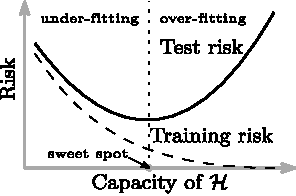
\includegraphics[width=0.5\textwidth,height=\textheight]{assets/u-shaped}
\caption{The so-called bias-variance trade-off represents a traditional
view of generalization consistent with uniform convergence bounds}
\end{figure}

The figure illustrates the traditional conception of the so-called
bias-variance trade-off. As model complexity increases the empirical
risk (training risk) decreases due to the model's improved ability to
interpolate the training data. However, increasing the model complexity
too far eventually leads to an increase in risk (test risk)
corresponding to signs of \emph{overfitting}.

This kind of picture has been drawn in numerous textbooks and courses on
machine learning. Of course, it does not seem to bear much resemblance
to what is observed in practice. We have already discussed the example
of the Perceptron which achieves zero training loss and still
generalizes well in theory. Numerous practitioners have observed that
other complex models also can simultaneously achieve close to zero
training loss and still generalize well. Moreover, in many cases risk
continues to decreases as model complexity grows and training data are
interpolated exactly down to (nearly) zero training loss. This empirical
relationship between overparameterization and risk appears to be robust
and manifests in numerous model classes, including overparameterized
linear models, ensemble methods, and neural networks.

\begin{figure}
\centering
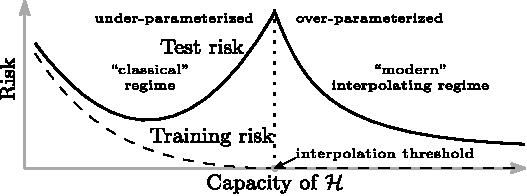
\includegraphics[width=1\textwidth,height=\textheight]{assets/doubledescent}
\caption{An extended picture with a ``double descent'' shape accounting
for the overparameterized regime.}
\end{figure}

In the absence of regularization and for certain model families, the
empirical relationship between model complexity and risk is more
accurately captured by the \emph{double descent} curve in the figure
above. There is an interpolation threshold at which a model of the given
complexity can fit the training data exactly. The complexity range below
the threshold is the \emph{underparameterized regime}, while the one
above is the overparameterized regime. Increasing model complexity in
the overparameterized regime continues to decrease risk indefinitely,
albeit at decreasing marginal returns, toward some convergence point.
The double descent curve is not universal. In many cases, in practice we
observe a single descent curve throughout the entire complexity range.
In other cases, we can see multiple bumps as we increase model
complexity.\footnote{Liang, Rakhlin, and Zhai, {``On the Multiple
  Descent of Minimum-Norm Interpolants and Restricted Lower Isometry of
  Kernels,''} in \emph{Conference on Learning Theory}, 2020.} However,
the general point remains: there is no evidence that highly
overparameterized models do not generalize. And, indeed, empirical
evidence suggests larger models not only generalize, but that larger
models make better out-of-sample predictors than smaller
ones.\footnote{He et al., {``Deep Residual Learning for Image
  Recognition,''} in \emph{Computer Vision and Pattern Recognition},
  2016; Huang et al., {``GPipe: Efficient Training of Giant Neural
  Networks Using Pipeline Parallelism,''} in \emph{Advances in Neural
  Information Processing Systems}, 2019.}

\hypertarget{optimization-versus-generalization}{%
\subsection{Optimization versus
generalization}\label{optimization-versus-generalization}}

Training neural networks with stochastic gradient descent, as is
commonly done in practice, attempts to solve a non-convex optimization
problem. Reasoning about non-convex optimization is known to be
difficult. As such theoreticians see a worthy goal in trying to prove
mathematically that stochastic gradient methods successfully minimize
the training objective of large artificial neural networks. The previous
chapter discussed some of the progress that has been made toward this
goal.

It is widely believed that what makes optimization easy crucially
depends on the fact that models in practice have many more parameters
than there are training points. While making optimization tractable,
overparameterization puts burden on generalization.

We can force a disconnect between optimization and generalization in a
simple experiment that we will see next. One consequence is that even if
a mathematical proof established the convergence guarantees of
stochastic gradient descent for training some class of large neural
networks, it would not necessarily on its own tell us much about why the
resulting model generalizes well to the test objective.

Indeed, consider the following experiment. Fix training data
\((x_1,y_1),\dots, (x_n, y_n)\) and fix a training algorithm~\(A\) that
achieves zero training loss on these data and achieves good test loss as
well.

Now replace all the labels~\(y_1,\dots,y_n\) by randomly and
independently drawn labels~\(\tilde y_1,\dots, \tilde y_n\). What
happens if we run the same algorithm on the training data with noisy
labels \((x_1,\tilde y_1),\dots, (x_n, \tilde y_n))\)?

\begin{figure}
\centering
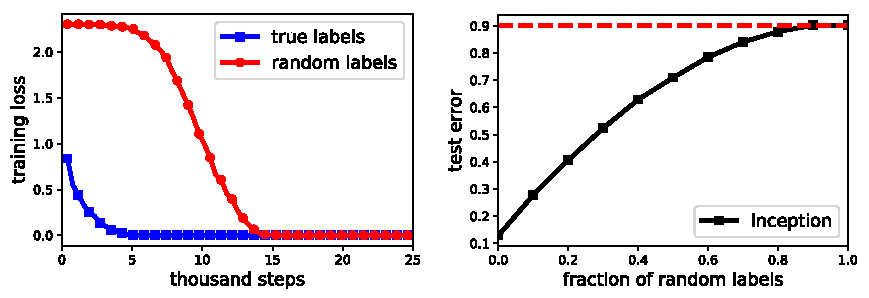
\includegraphics[width=1\textwidth,height=\textheight]{assets/randomization-test}
\caption{Randomization test on CIFAR-10. Left: How randomization affects
training loss. Training still converges to zero loss even on fully
randomized labels. Right: How increasing the fraction of corrupted
training labels affects classification error on the test set. At full
randomization, the test error degrades to \(90\%\), as good as guessing
one of the \(10\) classes.}
\end{figure}

One thing is clear. If we choose from~\(k\) discrete classes, we expect
the model trained on the random labels to have no more than~\(1/k\) test
accuracy, that is, the accuracy achieved by random guessing. After all
there is no statistical relationship between the training labels and the
test labels that the model could learn.

What is more interesting is what happens to optimization. The left panel
of the figure shows the outcome of this kind of \emph{randomization
test} on the popular CIFAR-10 image classification benchmark for a
standard neural network architecture. What we can see is that the
training algorithm continues to drive the training loss to zero even if
the labels are randomized. Moreover, the same is true for various other
kinds of randomizations. We can even replace the original images by
random pixels so as to get a randomly labeled random pixel images
\((\tilde x_i, \tilde y_i)\). The algorithm will continue to
successfully minimize the loss function.

The randomization experiment shows that optimization continues to work
well even when generalization performance is no better than random
guessing, i.e.,~\(10\%\) accuracy in the case of the CIFAR-10 benchmark
that has~\(10\) classes. The optimization method is moreover insensitive
to properties of the data, since it works even on random labels. A
consequence of this simple experiment is that a proof of convergence for
the optimization method may not reveal any insights into the nature of
generalization.

\hypertarget{the-diminished-role-of-explicit-regularization}{%
\subsection{The diminished role of explicit
regularization}\label{the-diminished-role-of-explicit-regularization}}

\index{regularization}

Regularization plays an important role in the theory of convex empirical
risk minimization. The most common form of regularization used to be
\(\ell_2\)-regularization corresponding to adding a scalar of the
squared Euclidean norm of the parameter vector to the objective
function.

\index{data augmentation}

A more radical form of regularization, called \emph{data augmentation},
is common in the practice of deep learning. Data augmentation transforms
each training point repeatedly throughout the training process by some
operation, such as a \emph{random crop} of the image. Training on such
randomly modified data points is meant to reduce overfitting, since the
model never encounters the exact same data point twice.

Regularization continues to be a component of training large neural
networks in practice. However, the nature of regularization is not
clear. We can see a representative empirical observation in the table
below.

\begin{longtable}[]{@{}ccccc@{}}
\caption{The training and test accuracy (in percentage) with and without
data augmentation and \(\ell_2\)-regularization on a representative
model architecture called \emph{Inception}. Explicit regularization
helps, but is not necessary for non-trivial generalization
performance.}\tabularnewline
\toprule
params & random crop & \(\ell_2\)-regularization & train accuracy & test
accuracy \\
\midrule
\endfirsthead
\toprule
params & random crop & \(\ell_2\)-regularization & train accuracy & test
accuracy \\
\midrule
\endhead
1,649,402 & yes & yes & 100.0 & 89.05 \\
& yes & no & 100.0 & 89.31 \\
& no & yes & 100.0 & 86.03 \\
& no & no & 100.0 & 85.75 \\
\bottomrule
\end{longtable}

The table shows the performance of a common neural model architecture,
called Inception, on the standard CIFAR-10 image classification
benchmark. The model has more than~\(1.5\) million trainable parameters,
even though there are only~\(50,000\) training examples spread
across~\(10\) classes. The training procedure uses two explicit forms of
regularization. One is a form of data augmentation with random crops.
The other is~\(\ell_2\)-regularization. With both forms of
regularization the fully trained model achieves close to~\(90\%\) test
accuracy. But even if we turn both of them off, the model still achieves
close to~\(86\%\) test accuracy (without even readjusting any
hyperparameters such as learning rate of the optimizer). At the same
time, the model fully interpolates the training data in the sense of
making no misclassification errors whatsoever on the training data.

These findings suggest that while explicit regularization may help
generalization performance, it is by no means necessary for strong
generalization of heavily overparameterized models.

\hypertarget{theories-of-generalization}{%
\section{Theories of generalization}\label{theories-of-generalization}}

With these empirical facts in hand, we now turn to mathematical theories
that might help explain what we observe in practice and also may guide
future empirical and theoretical work. In the remainder of the chapter,
we tour several different, seemingly disconnected views of
generalization.

We begin with a deep dive into \emph{algorithmic stability}, which
posits that generalization arises when models are insensitive to
perturbations in the data on which they are trained. We then discuss
\emph{VC dimension and Rademacher complexity}, which show how small
generalization gaps can arise when we restrict the complexity of models
we wish to fit to data. We then turn to \emph{margin bounds} which
assert that whenever the data is easily separable, good generalization
will occur. Finally we discuss generalization bounds that arise from
\emph{optimization}, showing how choice of an algorithmic scheme itself
can yield models with desired generalization properties.

In all of these cases, we show that we can recover generalization bounds
of the form we saw in the Perceptron: the bounds will decrease with
number of data points and increase with ``complexity'' of the optimal
prediction function. Indeed, looking back at the proof of the Perceptron
generalization bound, all of the above elements appeared. Our
generalization bound arose because we could remove single data points
from a set and not change the number of mistakes made by the Perceptron.
A large margin assumption was essential to get a small mistake bound.
The mistake bound itself was dependent on the iterations of the
algorithm. And finally, we related the size of the margin to the scale
of the data and optimal separator.

Though starting from different places, we will shows that the four
different views of generalization can all arrive at similar results.
Each of the aforementioned ingredients can alone lead to generalization,
but considerations of all of these aspects help to improve machine
learning methods. Generalization is multifaceted and multiple
perspectives are useful when designing data-driven predictive systems.

Before diving into these four different views, we first take a quick
pause to consider how we hope generalization bounds might look.

\hypertarget{how-should-we-expect-the-gap-to-scale}{%
\subsection{How should we expect the gap to
scale?}\label{how-should-we-expect-the-gap-to-scale}}

Before we turn to analyzing generalization gaps, it's worth first
considering how we should expect them to scale. That is, what is the
relationship between the expected size of~\(\Delta_{\mathrm{gen}}\) and
the number of observations,~\(n\)?

There are effectively two scaling regimes of interest in generalization
theory. In one case when the empirical risk is large, we expect the
generalization gap to decrease inversely proportional to~\(\sqrt{n}\).
When the empirical risk is expected to be very small, on the other hand,
we tend to see the the generalization gap decrease inversely
proportional to~\(n\).

Why we see these two regimes is illustrated by studying the behavior of
a \emph{single} prediction function~\(f\). Note that the zero-one loss
for a fixed function~\(f\) is a Bernoulli random variable, equal
to~\(1\) with probability~\(p\) and~\(1-p\) otherwise.~\(R_S\) is the
sample average of this random variable and~\(R\) is its expectation. To
estimate the generalization gap, we can apply Hoeffding's inequality to
find\\
\[
  \mathop\mathbb{P}[ R[f]-R_S[f] \geq \epsilon] \leq \exp\left( -2n\epsilon^2\right)\,.
\] Hence, we will have with probability~\(1-\delta\) on our sample that
\[
  |\Delta_{\mathrm{gen}}(f)| \leq \sqrt{\frac{\log(1/\delta)}{2n}}\,.
\] That is, the generalization gap goes to zero at a rate of
\(1/\sqrt{n}\).

In the regime where we observe no empirical mistakes, a more refined
analysis can be applied. Suppose that~\(R[f]>\epsilon\). Then the
probability that one observes~\(R_S=0\) can be bounded as \[
\begin{aligned}
  \mathop\mathbb{P}[ \forall i\colon\operatorname{sgn}(f(x_i))=y_i \mid R[f] > \epsilon]
  &= \prod_{i=1}^n \mathop\mathbb{P}[ \operatorname{sgn}(f(x_i))=y_i \mid R[f] > \epsilon] \\
  & \leq (1-\epsilon)^n \leq e^{-\epsilon n}\,.
  \end{aligned}
\] Hence, with probability~\(1-\delta\), \[
  |\Delta_{\mathrm{gen}}(f)| \leq \frac{\log(1/\delta)}{n}\,,  
\] which is the~\(1/n\) regime. These two rates are precisely what we
observe in the more complex regime of generalization bounds in machine
learning. The main trouble in difficulty in computing generalization
error is that our prediction function~\(f\) depends on the data, making
the above analysis inapplicable.

In this chapter, we will focus mostly on~\(1/\sqrt{n}\) rates. These
rates are more general as they make no assumptions about the expected
empirical risk. With a few notable exceptions, the derivation of
\(1/\sqrt{n}\) rates tends to be easier than the~\(1/n\) counterparts.
However, we note that every one of our approaches to generalization
bounds have analyses for the ``low empirical risk'' or ``large margin''
regimes. We provide references at the end of this chapter to these more
refined analyses.

\hypertarget{algorithmic-stability}{%
\section{Algorithmic stability}\label{algorithmic-stability}}

\index{stability!algorithmic}

We will first see a tight characterization in terms of an algorithmic
robustness property we call \emph{algorithmic stability}. Intuitively,
algorithmic stability measures how sensitive an algorithm is to changes
in a single training example. Whenever a model is insensitive to such
perturbations, the generalization gap will be small. Stability gives us
a powerful and intuitive way of reasoning about generalization.

There are a variety of different notions of perturbation. We could
consider resampling a single data point and look at how much a model
changes. We could also leave one data point out and see how much the
model changes. This was the heart of our Perceptron generalization
argument. More aggressively, we could study what happens when a single
data point is arbitrarily corrupted. All three of these approaches yield
similar generalization bounds, though it is often easier to work with
one than the others. To simplify the exposition, we choose to focus on
only one notion (resampling) here.

To introduce the idea of stability, we first condense our notation to
make the presentation a bit less cumbersome. Recall, that we operate on
tuples of~\(n\) labeled examples, \[
S=((x_1,y_1),\dots\dots,(x_n,y_n))\in(X\times Y)^n\,.
\] We let~\(z_i=(x_i,y_i)\) denote the~\(i\)-th labeled example pair. We
also will overload our notation and denote the loss accrued by a
prediction function~\(f\) on a data point~\(z\)
as~\(\mathit{loss}(f,z)\). That is,
\(\mathit{loss}(f,z) = \mathit{loss}(f(x),y)\).

With this notation in hand, let's now consider two independent samples
\(S = (z_1, \dots , z_n)\) and
\(S^{\prime} = (z^{\prime}_1, \dots ,z^{\prime}_{n})\), each drawn
independently and identically from the distribution~\(D\). We call the
second sample~\(S'\) a \emph{ghost sample} as it is solely an analytical
device. We never actually collect this second sample or run any
algorithm on it.

We introduce~\(n\) \emph{hybrid samples} \(S^{(i)}\),
for~\(i\in\{1, \dots, n\}\) as \[
S^{(i)} = (z_1, \,\dots ,\, z_{i-1}, \,z_{i}^{\prime},\, z_{i+1}, \,\dots \,,z_{n})\,,
\] where the~\(i\)-th example comes from~\(S',\) while all others come
from \(S.\)

We can now introduce a data-dependent notion of average stability of an
algorithm. For this definition, we think of an algorithm as a
deterministic map~\(A\) that takes a training sample
in~\((X\times Y)^n\) to some prediction function in a function
space~\(\Omega\). That is~\(A(S)\) denotes the function from~\(X\)
to~\(Y\) that is returned by our algorithm when run on the data
set~\(S\)

\index{stability!average}

\begin{Definition}

The \emph{average stability} of an algorithm
\(A\colon (X \times Y)^{n} \rightarrow \Omega\): \[
\Delta(A) = \mathop\mathbb{E}_{S,S^{\prime}}
\left[
\frac{1}{n}\sum_{i=1}^{n}
\left(\mathit{loss}(A(S),z_i^{\prime}) -\mathit{loss}(A(S^{(i)}),z_{i}^{\prime})\right)
\right]
\]

\end{Definition}

There are two useful ways to parse this definition. The first is to
interpret average stability as the average sensitivity of the algorithm
to a change in a single example. Since we don't know which of its~\(n\)
input samples the algorithm may be sensitive to, we test all of them and
average out the results.

Second, from the perspective of~\(A(S)\), the example~\(z_i^\prime\) is
\emph{unseen}, since it is not part of~\(S.\) But from the perspective
of \(A(S^{(i)})\) the example~\(z_i^\prime\) is seen, since it is part
of \(S^{(i)}\) via the substitution that defines the~\(i\)-th hybrid
sample. This shows that the instrument~\(\Delta(A)\) also measures the
average loss difference of the algorithm on seen and unseen examples. We
therefore have reason to suspect that average stability relates to
generalization gap as the next proposition confirms.

\begin{Proposition}

The expected generalization gap equals average stability: \[
\mathop\mathbb{E}[\Delta_{\mathrm{gen}}(A(S))] = \Delta(A)
\]

\end{Proposition}

\begin{Proof}

By linearity of expectation, \[
\begin{aligned}
\mathop\mathbb{E}[\Delta_{\mathrm{gen}}(A(S))]
&= \mathop\mathbb{E}\left[R[A(S)] - R_S[A(S)]\right] \\
&= \mathop\mathbb{E}\left[\frac{1}{n}\sum_{i=1}^{n}\mathit{loss}(A(S),z_i^{\prime})\right]
- \mathop\mathbb{E}\left[\frac{1}{n}\sum_{i=1}^{n}\mathit{loss}(A(S),z_i)\right]\,.
\end{aligned}
\] Here, we used that~\(z_i^\prime\) is an example drawn from the
distribution that does not appear in the set~\(S,\) while~\(z_i\) does
appear in~\(S.\) At the same time,~\(z_i\) and~\(z_i'\) are identically
distributed and independent of the other examples. Therefore, \[
\mathop\mathbb{E}\mathit{loss}(A(S),z_i) = \mathop\mathbb{E}\mathit{loss}(A(S^{(i)}),z_i^{\prime})\,.
\] Applying this identity to each term in the empirical risk above, and
comparing with the definition of~\(\Delta(A),\) we conclude \[
\mathop\mathbb{E}[R[A(S)] - R_S[A(S)]] = \Delta(A)
\]

\end{Proof}

\hypertarget{uniform-stability}{%
\subsection{Uniform stability}\label{uniform-stability}}

While average stability gave us an exact characterization of
generalization error, it can be hard to work with the expectation over
\(S\) and~\(S'.\) Uniform stability replaces the averages by suprema,
leading to a stronger but useful notion.

\index{stability!uniform}

\begin{Definition}

The \emph{uniform stability} of an algorithm~\(A\) is defined as \[
\Delta_{\mathrm{sup}}(A) = \sup_{\underset{d_H(S, S')=1}{S, S' \in (X\times Y)^n}}
\sup_{z\in(X\times Y)} |\mathit{loss}(A(S), z) - \mathit{loss}(A(S'), z)|,
\] where~\(d_H(S,S')\) denotes the Hamming distance between the
tuples~\(S\) and~\(S'\).

\end{Definition}

In this definition, it is important to note that the~\(z\) has nothing
to do with~\(S\) and~\(S'\). Uniform stability is effectively computing
the worst-case difference in the predictions of the learning algorithm
run on two arbitrary data sets that differ in exactly one point.

Uniform stability upper bounds average stability, and hence uniform
stability upper bounds generalization gap (in expectation). Thus, we
have the corollary \[
\mathop\mathbb{E}[\Delta_{\mathrm{gen}}(A(S))] \leq \Delta_{\mathrm{sup}} (A)
\]

This corollary turns out to be surprisingly useful since many algorithms
are uniformly stable. For example, strong convexity of the loss function
is sufficient for the uniform stability of empirical risk minimization,
as we will see next.

\hypertarget{stability-of-empirical-risk-minimization}{%
\subsection{Stability of empirical risk
minimization}\label{stability-of-empirical-risk-minimization}}

We now show that empirical risk minimization is uniformly stable
provided under strong assumptions on the loss function. One important
assumption we need is that the loss function~\(\mathit{loss}(w, z)\) is
differentiable and \emph{strongly convex} in the model parameters~\(w\)
for every example~\(z.\) What this means is that for every example~\(z\)
and for all~\(w,w'\in\Omega,\) \[
\mathit{loss}(w',z)\ge
\mathit{loss}(w,z)
+ \langle\nabla \mathit{loss}(w,z), w' - w\rangle
+ \frac{\mu}2\|w-w'\|^2
\] There's only one property of strong convexity we'll need. Namely, if
\(\Phi\colon\mathbb{R}^d\to\mathbb{R}\) is~\(\mu\)-strongly convex
and~\(w^*\) is a stationary point (and hence global minimum) of the
function~\(\Phi\), then we have \[
\Phi(w) - \Phi(w^*) \geq \frac{\mu}{2} \| w - w^* \|^2\,.
\] The second assumption we need is that~\(\mathit{loss}(w, z)\) is
\emph{\(L\)-Lipschitz} in~\(w\) for every~\(z\), i.e.,
\(\|\nabla \mathit{loss}(w, z)\|\le L\). Equivalently, this means
\(|\mathit{loss}(w, z)-\mathit{loss}(w',z)|\le L\|w-w'\|.\)

\begin{Theorem}

Assume that for every~\(z\),~\(\mathit{loss}(w, z)\) is~\(\mu\)-strongly
convex in~\(w\) over the domain~\(\Omega\), i.e., Further assume that,
that the loss function~\(\mathit{loss}(w, z)\) is~\(L\)-Lipschitz
in~\(w\) for every~\(z.\) Then, empirical risk minimization (ERM)
satisfies \[
\Delta_{\mathrm{sup}} (\text{ERM}) \leq \frac{4L^2}{\mu n}\,.
\]

\end{Theorem}

\begin{Proof}

Let
\(\hat w_S = \arg \min_{w\in \Omega} \frac{1}{n} \sum_{i=1}^n\mathit{loss}(w, z_i)\)
denote the empirical risk minimizer on the sample~\(S.\) Fix arbitrary
samples~\(S,S'\) of size~\(n\) that differ in a single index
\(i\in\{1,\dots,n\}\) where~\(S\) contains~\(z_i\) and~\(S'\)
contains~\(z_i'\). Fix an arbitrary example~\(z\). We need to show that
\[
|\mathit{loss}(\hat w_{S}, z) - \mathit{loss}(\hat w_{S'}, z)|
\leq \frac{4 L^2}{\mu n}\,.
\] Since the loss function is~\(L\)-Lipschitz, it suffices to show that
\[
\| \hat w_{S} - \hat w_{S'} \| \leq \frac{4L}{\mu n}\,.
\]

On the one hand, since~\(\hat w_S\) minimizes the empirical risk by
definition, it follows from the strong convexity of the empirical risk
that \[
\frac{\mu}{2} \| \hat w_{S} - \hat w_{S'} \|^2
\le R_S[\hat w_{S'}] - R_S[\hat w_{S}]\,.
\]

On the other hand, we can bound the right hand side as \[
\begin{aligned}
& R_S[\hat w_{S'}] - R_S[\hat w_{S}]\\
&=  \frac{1}{n} ( \mathit{loss}(\hat w_{S'}, z_i) - \mathit{loss}(\hat w_{S}, z_i)) + \frac{1}{n} \sum_{i \neq j} ( \mathit{loss}(\hat w_{S'}, z_j) - \mathit{loss}(\hat w_{S}, z_j))\\
&=\frac{1}{n} (\mathit{loss}(\hat w_{S'}, z_i) - \mathit{loss}(\hat w_{S}, z_i))
+ \frac{1}{n} (\mathit{loss}(\hat w_{S}, z_i') - \mathit{loss}(\hat w_{S'}, z_i'))
+ \left(R_{S'}[\hat w_{S'}] - R_{S'}[\hat w_{S}]\right)\\
&\leq \frac{1}{n} | \mathit{loss}(\hat w_{S'}, z_i) - \mathit{loss}(\hat w_{S}, z_i)| +
\frac{1}{n} |  \mathit{loss}(\hat w_{S}, z_i') - \mathit{loss}(\hat w_{S'}, z_i') |\\
&\leq  \frac{2 L}{n} \| \hat w_{S'} - \hat w_{S}\|\,.
\end{aligned}
\]

Here, we used the assumption that~\(\mathit{loss}\) is~\(L\)-Lipschitz
and the fact that \[
R_{S'}[\hat w_{S'}] - R_{S'}[\hat w_{S}] \leq 0\,.
\]

Putting together the strong convexity property and our calculation
above, we find \[
\| \hat w_{S'} - \hat w_{S} \| \leq \frac{4 L}{\mu n}\,.
\]

Hence,~\(\Delta_{\mathrm{sup}}(\text{ERM}) \leq \frac{4 L ^ 2}{\mu n}\).

\end{Proof}

An interesting point about this result is that there is no explicit
reference to the complexity of the model class referenced by~\(\Omega.\)

\hypertarget{stability-of-regularized-empirical-risk-minimization}{%
\subsection{Stability of regularized empirical risk
minimization}\label{stability-of-regularized-empirical-risk-minimization}}

\index{regularization}\index{regularized ERM}

Some empirical risk minimization problems, such as the Perceptron (ERM
with hinge loss) we saw earlier, are convex but not strictly convex. We
can turn convex problems into strongly convex problems by adding an
\emph{\(\ell_2\)-regularization} term to the loss function:

\[
r(w, z) = \mathit{loss}(w, z) + \frac{\mu}{2} \| w \|^2\,.
\]

The last term is named~\(\ell_2\)-regularization, \emph{weight decay},
or \emph{Tikhonov regularization} depending on field and
context.\index{weight decay}\index{Tikhonov regularization}

By construction, if the loss is convex, then the regularized loss
\(r(w, z)\) is~\(\mu\)-strongly convex. Moreover, we can typically
assume the loss is optimized over a compact domain. As a simple example,
consider the hinge loss for classification. Then we will have \[
  \frac{\mu}{2} \Vert w^*\Vert^2 \leq \mathop\mathbb{E}[r(0,z)]  = 1\,.
\] Hence no matter whether we minimize an empirical or population risk,
the optimal~\(w\) will have norm less than~\(\sqrt{2/\mu}\). If the data
are also bounded, say~\(\Vert x \Vert \leq D\), this means the loss is
Lipschitz as it has bounded derivatives on this compact set. Indeed, we
always have \[
  \Vert \nabla_w r(w,z) \Vert \leq D+\mu \|w\|\,.
\] Hence, we see that regularized empirical risk minimization will be
uniformly stable. Regularization gives us the following chain of
implications valid for convex empirical risk minimization:
Regularization and convexity together imply strong convexity, which
gives us uniform stability and thus generalization.

A simple argument further shows that solving the regularized objective
also solves the unregularized objective. The idea is that assuming
\(\|w\|\le B\) we can set the regularization parameter
\(\mu \approx \frac{L}{B\sqrt{n}}\). This ensures that the
regularization term~\(\mu\|w\|^2\) is at most~\(O(\frac{LB}{\sqrt{n}})\)
and therefore the minimizer of the regularized risk also minimizes the
unregularized risk up to error~\(O(\frac{LB}{\sqrt{n}})\). Plugging this
choice of~\(\mu\) into the ERM stability theorem, the generalization gap
will also be \(O(\frac{LB}{\sqrt{n}})\).

As a final observation, note that in the case where the data is linearly
separable with margin~\(\gamma\), we can recover a perceptron-like
generalization bound. Let~\(w_\gamma\) be a max-margin hyperplane for a
data set~\(S\) and~\(w_\star\) the minimizer of the empirical risk. We
know that the empirical loss will satisfy \[
R_S[w_\star] \leq R_S[w_\gamma] = \frac{\mu}{2} \| w_\gamma \|^2 = \frac{\mu }{2\gamma^2}\,.
\] Moreover, since we know that the hinge loss upper bounds the zero-one
loss, we have \[
Pr[Y w_\star^T X < 0] \leq R[w_\star] \leq R_S[w_\star] + \frac{4(D+\sqrt{2\mu})^2}{\mu n} \leq \frac{\mu }{2\gamma^2} +  \frac{4(D+\sqrt{2\mu})^2}{\mu n}\,.
\] Setting~\(\mu=\frac{2\gamma D}{\sqrt{n}}\) gives that \[
  Pr[Y w_\star^T X < 0] \leq \frac{ 3 D }{\gamma \sqrt{n}} + o(n^{-1/2})\,.
\] Up to lower order terms, this is proportional to the square root of
the bound we saw for the Perceptron in chapter 2. As we discussed
earlier, this rate is slower than the perceptron rate as it does not
explicitly take into account the fact that the empirical risk is zero.
However, it is worth noting that the relationship between the variables
in question---diameter, margin, and number of samples---precisely the
same as for the Perceptron, and we derived this bound as a simple lemma
of a much more general assertion. This bound is ubiquitous and we will
derive it several more times in this chapter.

Stability analysis combined with explicit regularization and convexity
thus give an appealing conceptual and mathematical approach to reasoning
about generalization. However, empirical risk minimization involving
non-linear models is increasingly successful in practice and generally
leads to non-convex optimization problems.

\hypertarget{model-complexity-and-uniform-convergence}{%
\section{Model complexity and uniform
convergence}\label{model-complexity-and-uniform-convergence}}

\index{uniform convergence}

We briefly review other useful tools to reason about generalization.
Arguably, the most basic is based on counting the number of different
functions that can be described with the given model parameters.

Given a sample~\(S\) of~\(n\) independent draws from the same underlying
distribution, the empirical risk~\(R_S[f]\) for a fixed function~\(f\)
is an average of~\(n\) random variables, each with mean equal to the
risk \(R[f]\). Assuming for simplicity that the range of our loss
function is bounded in the interval~\([0,1],\) Hoeffding's bound gives
us the tail bound \[
\mathop\mathbb{P}\left\{ R_S[f] > R[f] + t\right\} \le \exp(-2nt^2)\,.
\]

By applying the union bound to a finite set of functions~\(\mathcal{F}\)
we can guarantee that with probability~\(1-\delta,\) we have for all
functions~\(f\in\mathcal{F}\) that \[
\Delta_{\mathrm{gen}}(f)\le\sqrt{\frac{\ln|\mathcal{F}|+\ln(1/\delta)}{n}}\,.\quad\quad(1)
\]

The cardinality bound~\(|\mathcal{F}|\) is a basic measure of the
complexity of the model family~\(\mathcal{F}.\) We can think of the term
\(\ln(\mathcal{F})\) as a measure of complexity of the function class
\(\mathcal{F}\). The gestalt of the generalization bound as
``\(\sqrt{\mathrm{complexity}/n}\)'' routinely appears with varying
measures of complexity.

\hypertarget{vc-dimension}{%
\subsection{VC dimension}\label{vc-dimension}}

\index{VC dimension}

Bounding the generalization gap from above for all functions in a
function class is called \emph{uniform convergence}. A classical tool to
reason about uniform convergence is the Vapnik-Chervonenkis dimension
(VC dimension) of a function class
\(\mathcal{F}\subseteq X\rightarrow Y\), denoted
\(\mathrm{VC}(\mathcal{F})\). It's defined as the size of the largest
set \(Q\subseteq X\) such that for any Boolean function
\(h\colon Q \to \{-1,1\},\) there is a predictor~\(f\in\mathcal{F}\)
such that~\(f(x)= g(x)\) for all~\(x\in Q\). In other words, if there is
a size-\(d\) sample such that the functions of~\(\mathcal{F}\) induce
all \(2^d\) possible binary labelings of~\(S\), then the VC-dimension of
\(\mathcal{F}\) is at least~\(d\).

The VC-dimension measures the ability of the model class to conform to
an arbitrary labeling of a set of points. The so-called VC inequality
implies that with probability~\(1-\delta,\) we have for all functions
\(f\in\mathcal{F}\) \[
\Delta_{\mathrm{gen}}(f)\le \sqrt{\frac{\mathrm{VC}(\mathcal{F})\ln n+\ln(1/\delta)}{n}}\,.\quad\quad(2)
\]

We can see that the complexity term~\(\mathrm{VC}(\mathcal{F})\) refines
our earlier cardinality bound since
\(\mathrm{VC}(\mathcal{F})\le\log|\mathcal{F}|+1.\) However VC-dimension
also applies to infinite model classes. Linear models
over~\(\mathbb{R}^d\) have VC-dimension~\(d\), corresponding to the
number of model parameters. Generally speaking, VC dimension tends to
grow with the number of model parameters for many model families of
interest. In such cases, the bound in Equation 2 becomes useless once
the number of model parameters exceeds the size of the sample.

However, the picture changes significantly if we consider notions of
model complexity different than raw counts of parameters. Consider the
set of all hyperplanes in~\(\mathbb{R}^d\) with norm at
most~\(\gamma^{-1}\). Vapnik showed\footnote{Vapnik, \emph{Statistical
  Larning Theory} (Wiley, 1998).} that when the data had maximum norm
\(\|x\|\leq D\), then the VC dimension of this set of hyperplanes was
\(\frac{D^2}{\gamma^2}\). As described in a survey of support vector
machines by Burges, the worst case arrangement of~\(n\) data points is a
simplex in~\(n-2\) dimensions.\footnote{Burges, {``A Tutorial on Support
  Vector Machines for Pattern Recognition,''} \emph{Data Mining and
  Knowledge Discovery} 2, no. 2 (1998): 121--67.} Plugging this
VC-dimension into our generalization bound yields \[
\Delta_{\mathrm{gen}}(f)\le \sqrt{\frac{D^2\ln n+\gamma^2\ln(1/\delta)}{\gamma^2 n}}\,.
\] We again see our Perceptron style generalization bound! This bound
again holds when the empirical risk is nonzero. And the dimension of the
data,~\(d\) does not appear at all in this bound. The difference between
the parametric model and the margin-like bound is that we considered
properties of the data. In the \emph{worst case} bound which counts
parameters, it appears that high-dimensional prediction is impossible.
It is only by considering data-specific properties that we can find a
reasonable generalization bound.

\hypertarget{rademacher-complexity}{%
\subsection{Rademacher complexity}\label{rademacher-complexity}}

\index{Rademacher complexity}

An alternative to VC-dimension is Rademacher complexity, a flexible tool
that often is more amenable to calculations that incorporate
problem-specific aspects such as restrictions on the distribution family
or properties of the loss function. To get a generalization bound in
terms of Rademacher complexity, we typically apply the definition not
the model class~\(\mathcal{F}\) itself but to the class of functions
\(\mathcal{L}\) of the form~\(h(z) = \mathit{loss}(f, z)\) for some
\(f\in\mathcal{F}\) and a loss function~\(\ell.\) By varying the loss
function, we can derive different generalization bounds.

Fix a function class~\(\mathcal{L}\subseteq Z\to\mathbb{R}\), which will
later correspond to the composition of a predictor with a loss function,
which is why we chose the symbol~\(\mathcal{L}\). Think of the
domain~\(Z\) as the space of labeled examples~\(z=(x,y)\). Fix a
distribution~\(P\) over the space~\(Z\).

The \emph{empirical Rademacher complexity} of a function class
\(\mathcal{L}\subseteq Z\to\mathbb{R}\) with respect to a sample
\(Q=\{z_1,\dots,z_n\}\subseteq Z\) drawn i.i.d. from the
distribution~\(P\) is defined as: \[
\widehat{\mathfrak{R}}_n(\mathcal{L})
=\mathop\mathbb{E}_{\sigma\in\{-1,1\}^n}
\left[
\frac 1n \sup_{h\in\mathcal{L}}
\left|
\sum_{i=1}^n \sigma_i h(z_i)
\right|
\right]\,.
\]

We obtain the \emph{Rademacher complexity}
\(\mathfrak{R}_n(\mathcal{L})=\mathop\mathbb{E}\left[\widehat{\mathfrak{R}}_n(\mathcal{L})\right]\)
by taking the expectation of the empirical Rademacher complexity with
respect to the sample. Rademacher complexity measures the ability of a
function class to interpolate a random sign pattern assigned to a point
set.

One application of Rademacher complexity applies when the loss function
is~\(L\)-Lipschitz in the parameterization of the model class for every
example~\(z\). This bound shows that with probability~\(1-\delta\) for
all functions~\(f\in\mathcal{F},\) we have \[
\Delta_{\mathrm{gen}}(f)\le 2L{\mathfrak{R}}_n(\mathcal{F}) + 3\sqrt{\frac{\log(1/\delta)}{m}}\,.
\] When applied to the hinge loss with the function class being
hyperplanes of norm less than~\(\gamma^{-1}\), this bound again recovers
the perceptron generalization bound \[
\Delta_{\mathrm{gen}}(f)\le 2 \frac{D}{\gamma \sqrt{n}}
 + 3\sqrt{\frac{\log(1/\delta)}{n}}\,.
\]

\hypertarget{margin-bounds-for-ensemble-methods}{%
\section{Margin bounds for ensemble
methods}\label{margin-bounds-for-ensemble-methods}}

\index{boosting}\index{ensemble}\index{margin bounds}

Ensemble methods work by combining many weak predictors into one strong
predictor. The combination step usually involves taking a weighted
average or majority vote of the weak predictors. Boosting and random
forests are two ensemble methods that continue to be highly popular and
competitive in various settings. Both methods train a sequence of small
decision trees, each on its own achieving modest accuracy on the
training task. However, so long as different trees make errors that
aren't too correlated, we can obtain a higher accuracy model by taking,
say, a majority vote over the individual predictions of the trees.

Researchers in the 1990s already observed that boosting often continues
to improve test accuracy as more weak predictors are added to the
ensemble. The complexity of the entire ensemble was thus often far too
large to apply standard uniform convergence bounds.

A proffered explanation was that boosting, while growing the complexity
of the ensemble, also improved the \emph{margin} of the ensemble
predictor. Assuming that the final predictor~\(f\colon X\to \{-1,1\}\)
is binary, its \emph{margin} on an example~\((x,y)\) is defined as the
value~\(yf(x)\). The larger the margin the more ``confident'' the
predictor is about its prediction. A margin~\(yf(x)\) just above~\(0\)
shows that the weak predictors in the ensemble were nearly split evenly
in their weighted votes.

An elegant generalization bound relates the risk of any predictor~\(f\)
to the fraction of correctly labeled training examples at a given margin
\(\theta.\) Below let~\(R[f]\) be the risk of~\(f\) w.r.t.
classification error. However, let~\(R^\theta_S(f)\) be the empirical
risk with respect to \emph{margin errors} at level~\(\theta\), i.e., the
loss \(\mathbf{1}(yf(x)\le\theta)\) that penalizes errors where the
predictor is within an additive~\(\theta\) margin of making a mistake.

\begin{Theorem}

With probability~\(1-\delta\), every convex combination~\(f\) of base
classifiers in~\(\mathcal{H}\) satisfies the following bound for every
\(\theta>0:\)

\[
R[f]
- R^\theta_S[f]
\le O\left(
\frac1{\sqrt{n}}\left(\frac{
\mathrm{VC}(\mathcal{H})\log n}{\theta^2}
+\log(1/\delta)
\right)^{1/2}
\right)
\]

\end{Theorem}

The theorem can be proved using Rademacher complexity. Crucially, the
bound only depends on the VC dimension of the base class~\(\mathcal{H}\)
but not the complexity of ensemble. Moreover, the bound holds for all
\(\theta>0\) and so we can choose~\(\theta\) after knowing the margin
that manifested during training.

\hypertarget{margin-bounds-for-linear-models}{%
\subsection{Margin bounds for linear
models}\label{margin-bounds-for-linear-models}}

Margins also play a fundamental role for linear classification. We saw
one margin bound for linear models in our chapter on the Perceptron
algorithm. Similar bounds hold for other variants of linear
classification. We'll state the result here for a simple least squares
problem:

\[
w^* = \arg\min_{w\colon\|w\|\le B} \frac1n\sum_{i=1}^n\left(\langle x_i, w\rangle - y\right)^2
\]

In other words, we minimize the empirical risk w.r.t. the squared loss
over norm bounded linear separators, call this class~\(\mathcal{W}_B\).
Further assume that all data points satisfy~\(\|x_i\|\le 1\) and
\(y\in\{-1,1\}.\) Analogous to the margin bound in Theorem 2 it can be
shown that with probability~\(1-\delta\) for every linear
predictor~\(f\) specified by weights in~\(\mathcal{W}_B\) we have

\[
R[f]
- R_S^\theta[f]
\le 4\frac{{\mathfrak{R}}(\mathcal{W}_B)}{\theta}
+ O\left(\frac{\log(1/\delta)}{\sqrt{n}}\right)\,.
\]

Moreover, given the assumptions on the data and model class we made, the
Rademacher complexity satisfies
\({\mathfrak{R}}(\mathcal{W})\le B/\sqrt{n}.\) What we can learn from
this bound is that the relevant quantity for generalization is the ratio
of complexity to margin~\(B/\theta\).

It's important to understand that margin is a scale-sensitive notion; it
only makes sense to talk about it after suitable normalization of the
parameter vector. If the norm didn't appear in the bound we could scale
up the parameter vector to achieve any margin we want. For linear
predictors the Euclidean norm provides a natural and often suitable
normalization.

\hypertarget{generalization-from-algorithms}{%
\section{Generalization from
algorithms}\label{generalization-from-algorithms}}

In the overparameterized regime, there are always an infinite number of
models that minimize empirical risk. However, when we run a particular
algorithm, the algorithm usually returns only one from this continuum.
In this section, we show how directly analyzing algorithmic iteration
can itself yield generalization bounds.

\hypertarget{one-pass-optimization-of-stochastic-gradient-descent}{%
\subsection{One pass optimization of stochastic gradient
descent}\label{one-pass-optimization-of-stochastic-gradient-descent}}

As we briefly discussed in the optimization chapter, we can interpret
the convergence analysis of stochastic gradient descent as directly
providing a generalization bound for a particular variant of SGD. Here
we give the argument in full detail. Suppose that we choose a loss
function that upper bounds the number of mistakes. That is
\(\mathit{loss}(\hat{y},y) \geq \mathbb{1}\{y\hat{y}<0\}\). The hinge
loss would be such an example. Choose the function~\(R\) to be the risk
(not empirical risk!) with respect to this loss function: \[
    R[w] = \mathop\mathbb{E}[ \operatorname{loss}(w^T x, y) ]\,.
\] At each iteration, suppose we gain access to an example pair
\((x_i, y_i)\) sampled i.i.d. from the a data generating distribution.
Then when we run the stochastic gradient method, the iterates are \[
    w_{t+1} = w_t - \alpha_t e(w_t^Tx_t,y_t) x_t\,,
\] where \[
    e(z,y) = \frac{\partial \operatorname{loss}(z,y)}{\partial z}\,.
\] Suppose that for all~\(x\),~\(\Vert x \Vert \leq D\). Also suppose
that \(e(z,y)\leq C\). Then the SGD convergence theorem tells us that
after~\(n\) steps, starting at~\(w_0=0\) and using an appropriately
chosen constant step size, the average of our iterates~\(\bar{w}_n\)
will satisfy \[
\mathop\mathbb{P}[\operatorname{sign}(\bar{w}_n^T x ) \neq y ] \leq
\mathbb{E}[R[\bar{w}_n]] \leq R[w_\star]  + \frac{C D \Vert w_\star \Vert }{\sqrt{n}}\,.
\] This inequality tells us that we will find a distribution boundary
that has low \emph{population} risk after seeing~\(n\) samples. And the
population risk itself lets us upper bound the probability of our model
making an error on new data. That is, this inequality is a
generalization bound.

We note here that this importantly does not measure our empirical risk.
By running stochastic gradient descent, we can find a low-risk model
without ever computing the empirical risk.

Let us further assume that the population can be separated with large
margin. As we showed when we discussed the Perceptron, the margin is
equal to the inverse of the norm of the corresponding hyperplane.
Suppose we ran the stochastic gradient method using a hinge loss. In
this case,~\(C=1\), so, letting~\(\gamma\) denote the maximum margin, we
get the simplified bound \[
\mathop\mathbb{P}[\operatorname{sign}(\bar{w}_n^T x ) \neq y ] \leq
 \frac{D}{\gamma\sqrt{n}}\,.
\] Note that the Perceptron analysis did not have a step size parameter
that depended on the problem instance. But, on the other hand, this
analysis of SGD holds regardless of whether the data is separable or
whether zero empirical risk is achieved after one pass over the data.
The stochastic gradient analysis is more general but generality comes at
the cost of a looser bound on the probability of error on new examples.

\hypertarget{uniform-stability-of-stochastic-gradient-descent}{%
\subsection{Uniform stability of stochastic gradient
descent}\label{uniform-stability-of-stochastic-gradient-descent}}

Above we showed that empirical risk minimization is stable no matter
what optimization method we use to solve the objective. One weakness is
that the analysis applied to the exact solution of the optimization
problem and only applies for strongly convex loss function. In practice,
we might only be able to compute an approximate empirical risk minimizer
and may be interested in losses that are not strongly convex.
Fortunately, we can also show that some optimization methods are stable
even if they don't end up computing a minimizer of a strongly convex
empirical risk. Specifically, this is true for the stochastic gradient
method under suitable assumptions. Below we state one such result which
requires the assumption that the loss function is smooth.\footnote{A
  continuously differentiable function
  \(f\colon\mathbb{R}^d\to\mathbb{R}\) is~\(\beta\)-smooth if
  \(\|\nabla f(y)-\nabla f(x)\|\le \beta\|y-x\|.\)}

\begin{Theorem}

Assume a continuously differentiable loss function that is
\(\beta\)-smooth and~\(L\)-Lipschitz on every example and convex.
Suppose that we run the stochastic gradient method (SGM) with step sizes
\(\eta_t\le 2/\beta\) for~\(T\) steps. Then, we have \[
\Delta_{\mathrm{sup}} (\text{SGM}) \leq \frac{2L^2}{n}\sum_{t=1}^T\eta_t\,.
\]

\end{Theorem}

The theorem\footnote{Hardt, Recht, and Singer, {``Train Faster,
  Generalize Better: Stability of Stochastic Gradient Descent,''} in
  \emph{International Conference on Machine Learning}, 2016.} allows for
SGD to sample the same data points multiple times, as is common practice
in machine learning. The stability approach also extends to the
non-convex case albeit with a much weaker quantitative bound.

\hypertarget{what-solutions-does-stochastic-gradient-descent-favor}{%
\subsection{What solutions does stochastic gradient descent
favor?}\label{what-solutions-does-stochastic-gradient-descent-favor}}

We reviewed empirical evidence that explicit regularization is not
necessary for generalization. Researchers therefore believe that a
combination of data generating distribution and optimization algorithm
perform \emph{implicit regularization}. Implicit regularization
describes the tendency of an algorithm to seek out solutions that
generalize well on their own on a given a data set without the need for
explicit correction. Since the empirical phenomena we reviewed are all
based on gradient methods, it makes sense to study implicit
regularization of gradient descent. While a general theory for
non-convex problems remains elusive, the situation for linear models is
instructive.

Consider again the linear case of gradient descent or stochastic
gradient descent: \[
    w_{t+1} = w_t - \alpha e_t x_t
\] where~\(e_t\) is the gradient of the loss at the current prediction.
As we showed in the optimization chapter, if we run this algorithm to
convergence, we must have the resulting~\(\hat{w}\) lies in the span of
the data, and that it interpolates the data. These two facts imply that
the optimal~\(\hat{w}\) is the minimum Euclidean norm solution
of~\(Xw=y\). That is,~\(w\) solves the optimization problem \[
\begin{array}{ll}
    \text{minimize} & \|w\|^2\\
    \text{subject to} & y_i w^Tx_i = 1\,.
\end{array}
\] Moreover, a closed form solution of this problem is given by \[
    \hat{w}=X^T(XX^T)^{-1}y\,.
\] That is, when we run stochastic gradient descent we converge to a
very specific solution. Now what can we say about the generalization
properties of this minimum norm interpolating solution?

The key to analyzing the generalization of the minimum norm solution
will be a stability-like argument due to Liang and Recht.\footnote{Liang
  and Recht, {``Interpolating Classifiers Make Few Mistakes,''}
  \emph{arXiv:2101.11815}, 2021.} We aim to control the error of the
model trained on the first~\(m\) data points on the next data point in
the sequence, \(x_{m+1}\). To do so, we use a simple identity that
follows from linear algebra:

\begin{Lemma}

Let~\(S\) be an arbitrary set of~\(m\geq 2\) data points.
Let~\(w_{m-1}\) and \(w_{m}\) denote the minimum norm solution trained
on the first~\(m-1\) and \(m\) points respectively. Then \[
    (1-y_{m} \langle w_{m-1}, x_m \rangle)^2 = s_{m}^2 (\Vert| w_m \Vert|^2-\Vert| w_{m-1} \Vert|^2)\,,
\] where \[
    s_{m} := \operatorname{dist} \left(\operatorname{span}( \varphi_{x_1},\ldots, \varphi_{x_{m-1}}),\varphi_{x_{m}}\right)\,.
\]

\end{Lemma}

We hold off on proving this lemma and state and prove our generalization
result:

\begin{Theorem}

Let~\(S\) denote a set of~\(n\) i.i.d. samples from~\(\mathcal{D}\).
Let~\(S_j\) denote the first~\(j\) samples and~\(w_j\) denote the
solution of minimum norm that interpolates these~\(j\) points.
Let~\(D_j\) denote the maximum norm of~\(\Vert x_i \Vert\)
for~\(1\leq i\leq j\). Let~\((x,y)\) denote another independent sample
from~\(\mathcal{D}\). Then if
\(\epsilon_j:=\mathop\mathbb{E}[(1 - y f_{S_j}(x))^2]\) is a
non-increasing sequence, we have \[
    \mathop\mathbb{P}[ y \langle w_{n}, x \rangle < 0] \leq  \frac{\mathop\mathbb{E}[W(S_{n+1})^2 B(S_{n+1})^2]}{n}\,.
\]

\end{Theorem}

\begin{Proof}

Using the bound~\(s_i^2 \leq D_{n+1}^2\) and the lemma yields the
inequality \[
    \mathop\mathbb{E}[(1-y \langle w_i, x \rangle)^2] \leq D_{n+1}^2 (\mathop\mathbb{E}[\Vert| w_{i+1} \Vert|^2]-\mathop\mathbb{E}[\Vert w_i\Vert^2])\,.
\] Here, we could drop the subscript on~\(x\) and~\(y\) on the left-hand
side as they are identically distributed to~\((x_{i+1},y_{i+1})\).
Adding these inequalities together gives the bound \[
    \frac{1}{n} \sum_{i=1}^n \mathop\mathbb{E}[(1 - y f_{S_i}(x))^2]  \leq \frac{\mathop\mathbb{E}[W(S_{n+1})^2 B(S_{n+1})^2]}{n}\,.
\] Assuming the sequence is decreasing means that the minimum summand of
the previous inequality is~\(\mathop\mathbb{E}[(1 - y f_{i}(x))^2]\).
This and Markov's inequality prove the theorem.

\end{Proof}

This proof reveals that the minimum norm solution, the one found by
running stochastic gradient descent to convergence, achieves a nearly
identical generalization bound as the Perceptron, even with the fast
\(1/n\) rate. Here, nothing is assumed about margin, but instead we
assume that the complexity of the interpolating solution does not grow
rapidly as we increase the amount of data we collect. This proof
combines ideas from stability, optimization, and model complexity to
find yet another explanation for why gradient methods find high-quality
solutions to machine learning problems.

\hypertarget{proof-of-lemma}{%
\subsection{Proof of lemma}\label{proof-of-lemma}}

Let~\(K= XX^T\) denote the kernel matrix for~\(S\). Partition~\(K\) as
\[
    K = \begin{bmatrix} K_{11} & K_{12} \\ K_{21} & K_{22} \end{bmatrix}
\] where~\(K_{11}\) is~\((m-1) \times (m-1)\) and~\(K_{22}\) is a scalar
equal to~\(k(x_m,x_m)\). Similarly, partition the vector of labels~\(y\)
so that \(y^{(m-1)}\) denotes the first~\(m-1\) labels. Under this
partitioning, \[
 \langle w_{m-1} , x_m \rangle = K_{21} K_{11}^{-1} y^{(m-1)}\,.
\]

Now note that \[
s_m^2 = K_{22}-K_{21} K_{11}^{-1} K_{12}\,.
\] Next, using the formula for inverting partitioned matrices, we find
\[
    K^{-1} = \begin{bmatrix}
    (K_{11}-K_{12}K_{21}K_{22}^{-1})^{-1} & s_m^{-2} K_{11}^{-1} K_{12} \\
    s_m^{-2} (K_{11}^{-1} K_{12})^T & s_m^{-2}
    \end{bmatrix}\,.
\] By the matrix inversion lemma we have \[
    (K_{11}-K_{12}K_{21}K_{22}^{-1})^{-1}
    = K_{11}^{-1} +s_m^{-2} \left(K_{21} K_{11}^{-1}\right)^T\left(K_{21} K_{11}^{-1}\right) \,.
\] Hence, \[
    \Vert w_{i}\Vert = y^T K^{-1} y = s_m^{-2}(y_m^2 - 2y_m \langle w_{m-1} ,x_m\rangle +\langle w_{m-1} ,x_m\rangle^2 ) + {y^{(m-1)}}^T K_{11}^{-1} y^{(m-1)}\,.
\] Rearranging terms proves the lemma.

\hypertarget{looking-ahead}{%
\section{Looking ahead}\label{looking-ahead}}

Despite significant effort and many recent advances, the theory of
generalization in overparameterized models still lags behind the
empirical phenomenology. What governs generalization remains a matter of
debate in the research community.

Existing generalization bounds often do not apply directly to practice
by virtue of their assumptions, are quantitatively too weak to apply to
heavily overparameterized models, or fail to explain important empirical
observations. However, it is not just a lack of quantitative sharpness
that limits our understanding of generalization.

Conceptual questions remain open: What is it a successful theory of
generalization should do? What are formal success criteria? Even a
qualitative theory of generalization, that is not quantitatively precise
in concrete settings, may be useful if it leads to the successful
algorithmic interventions. But how do we best evaluate the value of a
theory in this context?

Our focus in this chapter was decidedly narrow. We discussed how to
related risk and empirical risk. This perspective can only capture
questions that relate performance on a sample to performance on the very
same distribution that the sample was drawn from. What is left out are
important questions of \emph{extrapolation} from a training environment
to testing conditions that differ from training. Overparameterized
models that generalize well in the narrow sense can fail dramatically
even with small changes in the environment. We will revisit the question
of generalization for overparameterized models in our chapter on deep
learning.

\hypertarget{chapter-notes-5}{%
\section{Chapter notes}\label{chapter-notes-5}}

The tight characterization of generalization gap in terms of average
stability, as well as stability of regularized empirical risk
minimization, is due to Shalev-Shwartz et al.\footnote{Shalev-Shwartz et
  al., {``Learnability, Stability and Uniform Convergence,''}
  \emph{JMLR} 11, no. Oct (2010): 2635--70.} Uniform stability was
introduced by Bousquet and Elisseeff.\footnote{Bousquet and Elisseeff,
  {``Stability and Generalization,''} \emph{JMLR} 2, no. Mar (2002):
  499--526.} For additional background on VC dimension and Rademacher
complexity, see, for example, the text by Shalev-Shwartz and
Ben-David.\footnote{Shalev-Shwartz and Ben-David, \emph{Understanding
  Machine Learning: From Theory to Algorithms} (Cambridge University
  Press, 2014).}

The double descent figure is from work of Belkin et al.\footnote{Belkin
  et al., {``Reconciling Modern Machine-Learning Practice and the
  Classical Bias{{}}variance Trade-Off,''} \emph{Proceedings of the
  National Academy of Sciences}, 2019.} Earlier work pointed out similar
empirical risk-complexity relationships.\footnote{Neyshabur, Tomioka,
  and Srebro, {``In Search of the Real Inductive Bias: On the Role of
  Implicit Regularization in Deep Learning,''} \emph{arXiv:1412.6614},
  2014.} The empirical findings related to the randomization test and
the role of regularization are due to Zhang et al.\footnote{Zhang et
  al., {``Understanding Deep Learning Requires Rethinking
  Generalization,''} in \emph{International Conference on Learning
  Representations}, 2017.}

Theorem 2 is due to Schapire et al.\footnote{Schapire et al.,
  {``Boosting the Margin: A New Explanation for the Effectiveness of
  Voting Methods,''} \emph{The Annals of Statistics} 26, no. 5 (1998):
  1651--86.} Later work showed theoretically that boosting maximizes
margin.\footnote{Zhang and Yu, {``Boosting with Early Stopping:
  Convergence and Consistency,''} \emph{The Annals of Statistics} 33
  (2005): 1538--79; Telgarsky, {``Margins, Shrinkage, and Boosting,''}
  in \emph{International Conference on Machine Learning}, 2013.}

The margin bound for linear models follows from more general results of
Kakade et al.\footnote{Kakade, Sridharan, and Tewari, {``On the
  Complexity of Linear Prediction: Risk Bounds, Margin Bounds, and
  Regularization,''} in \emph{Advances in Neural Information Processing
  Systems}, 2009, 793--800.} that build on earlier work by Bartlett and
Mendelson\footnote{Bartlett and Mendelson, {``Rademacher and Gaussian
  Complexities: Risk Bounds and Structural Results,''} \emph{JMLR} 3,
  no. Nov (2002): 463--82.} as well as work of Koltchinskii and
Panchenko.\footnote{Koltchinskii and Panchenko, {``Empirical Margin
  Distributions and Bounding the Generalization Error of Combined
  Classifiers,''} \emph{The Annals of Statistics} 30, no. 1 (2002):
  1--50.}

Rademacher complexity bounds for family of neural networks go back to
work of Bartlett\footnote{Bartlett, {``The Sample Complexity of Pattern
  Classification with Neural Networks: The Size of the Weights Is More
  Important Than the Size of the Network,''} \emph{Transactions on
  Information Theory} 44, no. 2 (1998): 525--36.} and remain and active
research topic. We will see more on this in our chapter on deep
learning.

See also\footnote{Hardt, Recht, and Singer, {``Train Faster, Generalize
  Better.''}} and subsequent work for attempts to explain the
generalization performance stochastic gradient descent in terms of its
stability properties. There has been an explosion of work on
generalization and overparameterization in recent years. See, also,
recent work exploring how other norms shed light on generalization
performance.\footnote{Neyshabur et al., {``Exploring Generalization in
  Deep Learning,''} in \emph{Advances in Neural Information Processing
  Systems}, 2017, 5947--56.}

Our exposition is by no means a representative survey of the broad
literature on this topic. There are several ongoing lines of work we did
not cover: PAC-Bayes bounds,\footnote{Dziugaite and Roy, {``Computing
  Nonvacuous Generalization Bounds for Deep (Stochastic) Neural Networks
  with Many More Parameters Than Training Data,''}
  \emph{arXiv:1703.11008}, 2017.} compression bounds,\footnote{Arora et
  al., {``Stronger Generalization Bounds for Deep Nets via a Compression
  Approach,''} \emph{arXiv:1802.05296}, 2018.} and arguments about the
properties of the optimization landscape.\footnote{Zhang et al.,
  {``Theory of Deep Learning {III}: Generalization Properties of Sgd''}
  (Discussion paper, Center for Brains, Minds; Machines (CBMM).
  Preprint, 2017).}

This chapter builds on a chapter by Hardt,\footnote{Hardt,
  {``Generalization in Overparameterized Models,''} in \emph{Beyond the
  Worst-Case Analysis of Algorithms}, ed. Tim Roughgarden (Cambridge
  University Press, 2021), 486--505.} but contains several structural
changes as well as different results.

\chapter{Deep learning}

The past chapters have sketched a path towards predictive modeling:
acquire data, construct a set of features that properly represent data
in a way such that relevant conditions can be discriminated, pose a
convex optimization problem that balances fitting training data to
managing model complexity, optimize this problem with a standard solver,
and then reason about generalization via the hold-out method or cross
validation. In many ways this pipeline suffices for most predictive
tasks.

However, this standard practice does have its deficiencies. Feature
engineering has many moving pieces, and choices at one part of the
pipeline may influence downstream decisions in unpredictable ways.
Moreover, different software dependencies may be required to intertwine
the various parts of this chain, making the machine learning engineering
more fragile. It's additionally possible that more concise feature
representations are possible if the pieces can all be tuned together.

Though motivated differently by different people, \emph{deep learning}
can be understood as an attempt to ``delayer'' the abstraction
boundaries in the standard machine learning workflow. It enables
holistic design of representation and optimization. This delayering
comes at the cost of loss of convexity and some theoretical guarantees
on optimization and generalization. But, as we will now describe in this
chapter, this cost is often quite modest and, on many machine learning
problems such as image classification and machine translation, the
predictive gains can be dramatic.

As the reader must be aware, deep learning has been tremendously
successful in pattern classification, and at the time of this writing is
the dominant approach to solving industrial machine learning problems
and is the top performing approach in most prediction tasks in computer
vision. There are a variety of sociotechnical explanations for why deep
learning has had such success. However, it's important to share with the
reader that the only honest answer for why you might want to prefer deep
learning over any other method is ``because it seems to work better on
certain problems and there is a lot of free software out there to run
the methods.'' We now retrace our path through representation,
optimization, and generalization, highlighting what is different for
Deep Learning and what remains the same.

\hypertarget{deep-models-and-feature-representation}{%
\section{Deep models and feature
representation}\label{deep-models-and-feature-representation}}

We discussed in the chapter on representation that template matching,
pooling, and nonlinear lifting can all be achieved by affine
transformations followed by pointwise nonlinearities. These mappings can
be chained together to give a series of new feature vectors: \[
    x_{\ell+1} = \phi(A_\ell x_\ell+b_\ell)\,.
\] Here,~\(\ell\) indexes the \emph{layer} of a model. We can chain
several layers together to yield a final representation~\(x_L\).

As a canonical example, suppose~\(x_1\) is a pixel representation of an
image. Let's say this representation has size
\(d_1 \times d_1 \times c_1\), with~\(d_1\) counting spatial dimensions
and \(c_1\) counting the number of color channels. We could
apply~\(c_2\) template matching convolutions to this image, resulting in
a second layer of size~\(d_1 \times d_1 \times c_2\). Since we expect
convolutions to capture local variation, we can compress the size of
this second layer, averaging every~\(2\times 2\) cell to produce~\(x_2\)
of size \(d_2 \times d_2 \times c_2\), with~\(d_2<d_1\) and~\(c_2>c_1\).
Repeating this procedure several times will yield a
representation~\(x_{L-1}\) which has few spatial dimensions (\(d_{L-1}\)
is small) but many channel dimensions (\(c_{L-1}\) is large). We can
then map this penultimate layer through some universal approximator like
a neural network.

A variety of machine learning pipelines can be thought of in this way.
The first layer might correspond to edge detectors like in
SIFT\footnote{Lowe, {``Distinctive Image Features from Scale-Invariant
  Keypoints,''} \emph{International Journal of Computer Vision} 60, no.
  2 (2004): 91--110.} or HOG.\footnote{Dalal and Triggs, {``Histograms
  of Oriented Gradients for Human Detection,''} in \emph{Computer Vision
  and Pattern Recognition}, 2005.} The second layer may look for parts
relevant to detection like in a deformable parts model.\footnote{Felzenszwalb
  et al., {``Object Detection with Discriminatively Trained Part-Based
  Models,''} \emph{{IEEE} Transactions on Pattern Analysis and Machine
  Intelligence} 32, no. 9 (2009): 1627--45.} The insight in deep
learning is that we can declare the parameters of each layer~\(A_\ell\)
and~\(b_\ell\) to be \emph{optimization variables}. This way, we do not
have to worry about the particular edge or color detectors to use for
our problem, but can instead let the collected data dictate the best
settings of these features.

This abstraction of ``features'' as ``structure linear maps with tunable
parameters'' allows for a set of basic building blocks that can be used
across a variety of domains.

\begin{enumerate}
\def\labelenumi{\arabic{enumi}.}
\item
  \textbf{Fully connected layers.} Fully connected layers are simply
  unstructured neural networks that we discussed in the representation
  chapter. For a fixed nonlinear function~\(\sigma\), a fully connected
  layer maps a vector~\(x\) to a vector~\(z\) with coordinates \[
   z_{i} = \sigma\left(\sum_j A_{ij}x_j + b_i\right)\,.
  \] While it is popular to chain fully connected layers together to get
  deep neural networks, there is little established advantage over just
  using a single layer. Daniely et al.~have backed up this empirical
  observation, showing theoretically that no new approximation power is
  gained by concatenating fully connected layers.\footnote{Daniely,
    Frostig, and Singer, {``Toward Deeper Understanding of Neural
    Networks.''}} Moreover, as we will discuss below, concatenating many
  layers together often slows down optimization. As with most things in
  deep learning, there's nothing saying you can't chain fully connected
  layers, but we argue that most of the gains in deep learning come from
  the structured transforms, including the ones we highlight here.
\item
  \textbf{Convolutions}. Convolutions are the most important building
  block in all of deep learning. We have already discussed the use of
  convolutions as template matchers that promote spatial invariances.
  Suppose the input is~\(d_0 \times d_0 \times c_0\), with the first two
  components indexing space and the last indexing channels. The
  parameter~\(A\) has size~\(q_0 \times q_0 \times c_0 \times c_1\),
  where \(q_0\) is usually small (greater than~\(2\) and less
  than~\(10\).~\(b\) typically has size~\(c_1\). The number of
  parameters used to define a convolutional layer is dramatically
  smaller than what would be used in a fully connected layer. The
  structured linear map of a convolution can be written as \[
   z_{a,b,c} = \sigma\left( \sum_{i,j,k} A_{i,j,k,c} x_{a-i,b-j,k} + b_{c} \right)\,.
  \]
\item
  \textbf{Recurrent structures.} Recurrent structures let us capture
  repeatable stationary patters in time or space. Suppose we expect
  stationarity in time. In this case, we expect each layer to represent
  a state of the system, and the next time step should be a static
  function of the previous: \[
   x_{t+1} = f(x_t)
  \] When we write~\(f\) as a neural network, this is called a
  \emph{recurrent neural network}. Recurrent neural networks \emph{share
  weights} insofar as the~\(f\) does not change from one time step to
  the next.
\item
  \textbf{Attention mechanisms.} Attention mechanisms have proven
  powerful tools in natural language processing for collections of
  vectors with dependencies that are not necessarily sequential. Suppose
  our layer is a list of~\(m\) vectors of dimension~\(d\). That
  is,~\(x\) has shape \(d\times m\). An attention layer will have two
  matrices~\(U\) and~\(V\), one to operate on the feature dimensions and
  one to operate on the sequential dimensions. The transformation takes
  form \[
   z_{a,b} = \sigma\left( \sum_{i,j} U_{a,i} x_{ij} V_{b,j} \right)\,.
  \] Just as was the case with convolutions, this structured map can
  have fewer dimensions than a fully connected layer, and can also
  respect a separation of the feature dimensions from the sequential
  dimensions in the data matrix~\(x\).
\end{enumerate}

\hypertarget{optimization-of-deep-nets}{%
\section{Optimization of deep nets}\label{optimization-of-deep-nets}}

Once we have settled on a feature representation, typically called
\emph{model architecture} in this context, we now need to solve
empirical risk minimization. Let's group all of the parameters of the
layers into a single large array of weights,~\(w\). We denote the map
from~\(x\) to prediction with weights~\(w\) as~\(f(x;w)\). Then at an
abstract level, empirical risk minimization amounts to minimizing \[
    R_S[w] = \frac{1}{n}\sum_{i=1}^n \mathit{loss}(f(x_i;w),y_i)
\] This is a nonconvex optimization problem, but we can still run
gradient methods to try to find minimizers. Our main concerns from an
optimization perspective are whether we run into local optima and how
can we compute gradient steps efficiently.

We will address gradient computation through a discussion of automatic
differentiation. With regards to global optimization, there are
unfortunately computational complexity results proving efficient
optimization of arbitrary neural networks is intractable. Even neural
nets with a single neuron can have exponentially many local
minimizers,\footnote{Auer, Herbster, and Warmuth, {``Exponentially Many
  Local Minima for Single Neurons,''} in \emph{Advances in Neural
  Information Processing Systems}, 1996.} and finding the minimum of a
simple two-layer neural network is NP-hard.\footnote{Vu, {``On the
  Infeasibility of Training Neural Networks with Small Mean-Squared
  Error,''} \emph{Transactions on Information Theory} 44, no. 7 (1998):
  2892--2900; Goel et al., {``Tight Hardness Results for Training
  Depth-2 ReLU Networks,''} in \emph{Innovations in Theoretical Computer
  Science}, 2021.} We cannot expect a perfectly clean mathematical
theory guiding our design and implementation of neural net optimization
algorithms.

However, these theoretical results are \emph{worst case}. In practice,
optimization of neural nets is quite easy. If the loss is bounded below
by zero, any model with zero loss is a global minimizer. As we discussed
in the generalization chapter, one can quickly find a global optimum of
a state-of-the-art neural net by cloning a github repo and turning off
the various regularization schemes. In this section, we aim to provide
some insights about the disconnect between the computational complexity
pessimism and the results achieved in practice. We provide some partial
insights as to why neural net optimization is easy by studying the
convergence of the predictions and how this convergence can be aided by
overparameterization.

\hypertarget{convergence-of-predictions-in-nonlinear-models}{%
\subsection{Convergence of predictions in nonlinear
models}\label{convergence-of-predictions-in-nonlinear-models}}

Consider the special case where we aim to minimize the square-loss. Let
\(\hat{y}_t\) denote the vector of predictions~\(\{f(x_i;w_t)\}\). Then
gradient descent follows the iterations \[
    w_{t+1} = w_t - \alpha \mathsf{D}_w f(x;w_t) (\hat{y}_t - y)
\] where~\(\mathsf{D}_w f(x;w_t)\) denotes the~\(d\times n\) Jacobian
matrix of the predictions~\(\hat{y}_t\). Reasoning about convergence of
the weights is difficult, but we showed in the optimization chapter that
we could reason about convergence of the predictions: \[
    \hat{y}_{t+1}-y = (I -  \alpha \mathsf{D}_w f(x; w_t)^T \mathsf{D}_w f(x;w_t))(\hat{y}_t - y) + \alpha \epsilon_t\,.
\] Here, \[
    \epsilon_t = \frac{\alpha}{2} \Lambda \Vert \hat{y}_t - y \Vert^2
\] and~\(\Lambda\) bounds the curvature of the~\(f\).
If~\(\epsilon_t=0\) is sufficiently small the predictions will converge
to the training labels.

Hence, under modest assumptions, nonconvexity does not stand in the way
of convergence to an empirical risk minimizer. Moreover, control of the
Jacobians~\(\mathsf{D}_w f\) can accelerate convergence. We can derive
some reasonable ground rules on how to keep~\(\mathsf{D}_w f\) well
conditioned by unpacking how we compute gradients of compositions of
functions.

\hypertarget{automatic-differentiation}{%
\subsection{Automatic differentiation}\label{automatic-differentiation}}

For linear models it's easy to calculate the gradient with respect to
the model parameters analytically and to implement the analytical
expression efficiently. The situation changes once we stack many
operations on top of each other. Even though in principle we can
calculate gradients using the chain rule, this gets tedious and
error-prone very quickly. Moreover, the straightforward way of
implementing the chain rule is computationally inefficient. What's worse
is that any change to the model architecture would require us to redo
our calculation and update its implementation.

Fortunately, the field of \emph{automatic differentiation} has the tools
to avoid all of these problems. At a high-level, automatic
differentiation provides efficient algorithms to compute gradients of
any function that we can write as a composition of differentiable
building blocks. Though automatic differentiation has existed since the
1960s, the success of deep learning has led to numerous free,
well-engineered, and efficient automatic differentiation packages.
Moreover, the dynamic programming algorithm behind these methods is
quite instructive as it gives us some insights into how to best engineer
model architectures with desirable gradients.

Automatic differentiation serves two useful purposes in deep learning.
First, it lowers the barrier to entry, allowing practitioners to think
more about modeling than about the particulars of calculus and numerical
optimization. Second, a standard automatic differentiation algorithm
helps us write down parseable formulas for the gradients of our
objective function so we can reason about what structures encourage
faster optimization.

To define this dynamic programming algorithm, called
\emph{backpropagation}\index{backpropagation}, it's helpful to move up a
level of abstraction before making the matter more concrete again. After
all, the idea is completely general and not specific to deep models.
Specifically, we consider an abstract computation that proceeds in~\(L\)
steps starting from an input~\(z^{(0)}\) and produces an output
\(z^{(L)}\) with~\(L-1\) intermediate steps~\(z^{(1)},\dots,z^{(L-1)}\):
\[
\begin{aligned}
  \text{input}\quad z^{(0)}\\
    z^{(1)} &= f_1(z^{(0)})\\
     &\vdots\\
    z^{(L-1)} &= f_{L-1}(z^{(L-2)})\\
\text{output}\quad z^{(L)} &=f_L(z^{(L-1)})
\end{aligned}
\] We assume that each \emph{layer} \(z^{(i)}\) is a real-valued vector
and that each function~\(f_i\) maps a real-valued vector of some
dimension to another dimension. Recall that for a
function~\(f\colon\mathbb{R}^n\to\mathbb{R}^m\), the Jacobian
matrix~\(\mathsf{D}(w)\) is the~\(n\times m\) matrix of first-order
partial derivatives evaluated at the point~\(w\). When~\(m=1\) the
Jacobian matrix coincides with the transpose of the gradient.

In the context of backpropagation, it makes sense to be a bit more
explicit in our notation. Specifically, we will denote the Jacobian of a
function~\(f\) with respect to a variable~\(x\) evaluated at point~\(w\)
by \(\mathsf{D}_x f(w)\,.\)

The backpropagation algorithm is a computationally efficient way of
computing the partial derivatives of the output~\(z^{(L)}\) with respect
to the input~\(z^{(0)}\) evaluated at a given parameter vector~\(w\),
that is, the Jacobian~\(\mathsf{D}_{z^{(0)}} z^{(L)}(w).\) Along the
way, it computes the Jacobians for any of the intermediate layers as
well.

\begin{Algorithm}

\textbf{Backpropagation}

\begin{itemize}
\tightlist
\item
  Input: parameters \(w\)
\item
  Forward pass:

  \begin{itemize}
  \tightlist
  \item
    Set \(v_0 = w\)
  \item
    For \(i =1,\ldots,L\):

    \begin{itemize}
    \tightlist
    \item
      Store \(v_{i-1}\) and compute \(v_i = f_i(v_{i-1})\)
    \end{itemize}
  \end{itemize}
\item
  Backward pass:

  \begin{itemize}
  \tightlist
  \item
    Set \(\Lambda_L = \mathsf{D}_{z_{L}} z_L(v_L)= I\).
  \item
    For \(i=L,\ldots,1\):

    \begin{itemize}
    \tightlist
    \item
      Set
      \(\Lambda_{i-1} =\Lambda_i\mathsf{D}_{z^{(i-1)}} z^{(i)}(v_{i-1})\).
    \end{itemize}
  \end{itemize}
\item
  Output \(\Lambda_0\).
\end{itemize}

\end{Algorithm}

First note that backpropagation runs in time~\(O(LC)\) where~\(C\) is
the computational cost of performing an operation at one step. On the
forward pass, this cost correspond to function evaluation. On the
backward pass, it requires computing the partial derivatives of
\(z^{(i)}\) with respect to~\(z^{(i-1)}\). The computational cost
depends on what the operation is. Typically, the~\(i\)-th step of the
backward pass has the same computational cost as the
corresponding~\(i\)-th step of the forward pass up to constant factors.
What is important is that computing these partial derivatives is an
entirely \emph{local} operation. It only requires the partial
derivatives of a function with respect to its input evaluated at the
value~\(v_{i-1}\) that we computed in the forward pass. This observation
is key to all fast implementations of backpropagation. Each operation in
our computation only has to implement function evaluation, its
first-order derivatives, and store an array of values computed in the
forward pass. There is nothing else we need to know about the
computation that comes before or after.

The main correctness property of the algorithm is that the final output
\(\Lambda_0\) equals the partial derivative of the output layer with
respect to the input layer evaluated at the input~\(w\).

\begin{Proposition}

\textbf{Correctness of backpropagation.} \[
\Lambda_0 = \mathsf{D}_{z^{(0)}} z^{(L)}(w)
\]

\end{Proposition}

The claim directly follows by induction from the following lemma, which
states that if we have the correct partial derviatives at step~\(i\) of
the backward pass, then we also get them at step~\(i-1.\)

\begin{Lemma}

\textbf{Backpropagation invariant.} \[
\Lambda_i = \mathsf{D}_{z^{(i)}} z^{(L)}(v_i)
\quad\Longrightarrow\quad
\Lambda_{i-1} = \mathsf{D}_{z^{(i-1)}} z^{(L)}(v_{i-1})
\]

\end{Lemma}

\begin{Proof}

Assume that the premise holds. Then, we have \[
\begin{aligned}
\Lambda_{i-1}
&=  \Lambda_i\mathsf{D}_{z^{(i-1)}} z^{(i)}(v_{i-1}) \\
& = \mathsf{D}_{z^{(i)}} z^{(L)}(v_i)
    \mathsf{D}_{z^{(i-1)}} z^{(i)}(v_{i-1}) \\
& = \mathsf{D}_{z^{(i-1)}} z^{(L)}(v_{i-1}) \\
\end{aligned}
\] The last identity is the multivariate chain rule.\marginnote{To aid
the intuition read this as
\[\frac{\partial z^{(L)}}{\partial z^{(i)}}\frac{\partial z^{(i)}}{\partial z^{(i-1)}}
  =\frac{\partial z^{(L)}}{\partial z^{(i-1)}}\]}

\end{Proof}

\hypertarget{a-worked-out-example}{%
\subsection{A worked out example}\label{a-worked-out-example}}

The backpropagation algorithm works in great generality. It produces
partial derivatives for any variable appearing in any layer~\(z^{(i)}\).
So, if we want partial derivatives with respect to some parameters, we
only need to make sure they appear on one of the layers. This
abstraction is so general that we can easily express all sorts of deep
architectures and the associated objective functions with it.

But let's make that more concrete and get a feeling for the mechanics of
backpropagation in the two cases that are most common: a non-linear
transformation applied coordinate-wise, and a linear transformation.

Suppose at some point in our computation we apply the \emph{rectified
linear unit} \(\mathrm{ReLU}=\max\{u, 0\}\) coordinate-wise to the
vector~\(u\). ReLU units remain one of the most common non-linearities
in deep neural networks. To implement the backward pass, all we need to
be able to do is to compute the partial derivatives
of~\(\mathrm{ReLU}(u)\) with respect to~\(u\). It's clear that
when~\(u_i > 0\), the derivative is~\(1\). When \(u_i < 0,\) the
derivative is~\(0\). The derivative is not defined at \(u_i=0,\) but we
choose to ignore this issue by setting it to be \(0\).\marginnote{Many
operations appearing in modern deep models are not everywhere
differentiable.} The resulting Jacobian matrix is a diagonal matrix
\(D(u)\) which has a one in all coordinates corresponding to positive
coordinates of the input vector, and is zero elsewhere.

\begin{itemize}
\tightlist
\item
  Forward pass:

  \begin{itemize}
  \tightlist
  \item
    Input: \(u\)
  \item
    Store \(u\) and compute the value \(v=\mathrm{ReLU}(u)\).
  \end{itemize}
\item
  Backward pass:

  \begin{itemize}
  \tightlist
  \item
    Input: Jacobian matrix \(\Lambda\)
  \item
    Output \(\Lambda D(u)\)
  \end{itemize}
\end{itemize}

If we were to swap out the rectified linear unit for some other
coordinate-wise nonlinearity, we'd still get a diagonal matrix. What
changes are the coefficients along the diagonal.

Now, let's consider an affine transformation of the input~\(v=Au + b\).
The Jacobian of an affine transformation is simply the matrix~\(A\)
itself. Hence, the backward pass is simple:

\begin{itemize}
\tightlist
\item
  Backward pass:

  \begin{itemize}
  \tightlist
  \item
    Input: Jacobian matrix \(\Lambda\)
  \item
    Output: \(\Lambda A\)
  \end{itemize}
\end{itemize}

We can now easily chain these together. Suppose we have a typical ReLU
network that strings together~\(L\) linear transformations with ReLU
operations in between: \[
f(x)=A_L\mathrm{ReLU}(A_{L-1}\mathrm{ReLU}(\cdots \mathrm{ReLU}(A_1x)))
\] The Jacobian of this chained operation with respect to the
input~\(x\) is given by a chain of linear operations: \[
A_LD_{L-1}A_{L-1}\cdots D_1A_1
\] Each matrix~\(D_i\) is a diagonal matrix that zeroes out some
coordinates and leaves others untouched. Now, in a deep model
architecture the weights of the linear transformation are typically
trainable. That means we really want to be able to compute the gradients
with respect to, say, the coefficients of the matrix~\(A_i\).

Fortunately, the same reasoning applies. All we need to do is to make
\(A_i\) part of the input to the matrix-vector multiplication node and
backpropagation will automatically produce derivatives for it. To
illustrate this point, suppose we want to compute the partial
derivatives with respect to, say, the~\(j\)-th column of~\(A_i\). Let
\(u=\mathrm{ReLU}(A_{i-1}\cdots (A_1x))\) be the vector that we multiply
\(A_i\) with. We know from the argument above that the Jacobian of the
output with respect to the vector~\(A_iu\) is given by the linear map
\(B=A_LD_{L-1}A_{L-1}\cdots D_i\). To get the Jacobian with respect to
the \(j\)-th column of~\(A_i\) we therefore only need to find the
partial derivative of~\(A_iu\) with respect to the~\(j\)-th column
of~\(A_i\). We can verify by taking derivatives that this
equals~\(u_jI\). Hence, the partial derivatives of~\(f(x)\) with respect
to the~\(j\)-th column of~\(A_i\) are given by~\(Bu_j\).

Let's add in the final ingredient, a loss function. Suppose~\(A_L\) maps
into one dimension and consider the squared loss~\(\frac12(f(x)-y)^2.\)
The only thing this loss function does is to scale our Jacobian by a
factor~\(f(x)-y.\) In other words, the partial derivatives of the loss
with respect to the~\(j\)-th columns of the weight matrix~\(A_i\) is
given by~\((f(x)-y)Bu_j\).

As usual with derivatives, we can interpret this quantity as the
\emph{sensitivity} of our loss to changes in the model parameters. This
interpretation will be helpful next.

\hypertarget{vanishing-gradients}{%
\section{Vanishing gradients}\label{vanishing-gradients}}

The previous discussion revealed that the gradients of deep models are
produced by chains of linear operations. Generally speaking, chains of
linear operations tend to either blow up the input exponentially with
depth, or shrink it, depending on the singular values of the matrices.
It is helpful to keep in mind the simple case of powering the same
symmetric real matrix~\(A\) a number of times. For almost all
vectors~\(u\), the norm~\(\|A^Lu\|\) grows
as~\(\Theta\left(\lambda_1(A)^L\right)\) asymptotically with~\(L\).
Hence it vanishes exponentially quickly if \(\lambda_1(A)<1\) and it
grows exponentially quickly if~\(\lambda_1(A)>1.\)

When it comes to gradients, these two cases correspond to the
\emph{vanishing gradients problem} and the \emph{exploding gradients
problem}, respectively. Both result in a failure case for gradient-based
optimization methods. Huge gradients are numerically unstable. Tiny
gradients preclude progress and stall any gradient-based optimization
method. We can always avoid one of the problems by scaling the weights,
but avoiding both can be delicate.

Vanishing and exploding gradients are not the fault of an optimization
method. They are a property of the model architecture. As a result, to
avoid them we need to engineer our model architectures carefully. Many
architecture innovations in deep learning aim to address this problem.
We will discuss two of them. The first are residual connections, and the
second are layer normalizations.

\hypertarget{residual-connections}{%
\subsection{Residual connections}\label{residual-connections}}

The basic idea behind \emph{residual networks} is to make each layer
close to the identity map. Traditional building blocks of neural
networks typically looked like two affine transformations~\(A, B\), with
a nonlinearity in the middle: \[
f(x)= B(\mathrm{ReLU}(A(x)))
\] Residual networks modify these building blocks by adding the input
\(x\) back to the output: \[
h(x)= x + B(\mathrm{ReLU}(A(x)))
\] In cases where the output of~\(C\) differs in its dimension
from~\(x\), practitioners use different padding or truncation schemes to
match dimensions. Thinking about the computation graph, we create a
connection from the input to the output of the building block that
\emph{skips} the transformation. Such connections are therefore called
\emph{skip connections}.

This seemingly innocuous change was hugely successful. Residual networks
took the computer vision community by storm, after they achieved leading
performance in numerous benchmarks upon their release in 2015. These
networks seemed to avoid the vanishing gradients better than prior
architectures and allowed for model depths not seen before.

Let's begin to get some intuition for why residual layers are reasonable
by thinking about what they do to the gradient computation. Let
\(J = \mathsf{D}_x f(x)\) be the Jacobian of the function~\(f\) with
respect to its input. We can verify that the Jacobian of the residual
block looks like \[
J' = \mathsf{D}_x h(x) = \mathsf{D}_x I(x) + \mathsf{D}_x f(x) = I + J\,.
\] In other words, the Jacobian of a residual block is the Jacobian of a
regular block plus the identity. This means that if we scale down the
weights of the regular block, the Jacobian~\(J'\) approaches the
identity in the sense that all its singular values are
between~\(1-\epsilon\) and \(1+\epsilon\). We can think of such a
transformation as locally well-conditioned. It neither blows up nor
shrinks down the gradient much. Since the full Jacobian of a deep
residual network will be a product of such matrices, our reasoning
suggests that suitably scaled residual networks have well-conditioned
Jacobians, and hence, as we discussed above, predictions should converge
rapidly.

Our analyses of non-convex ERM thus far have described scenarios where
we could prove the \emph{predictions} converge to the training labels.
Residual networks are interesting as we can construct cases where
\emph{the weights} converge to a unique optimal solution. This perhaps
gives even further motivation for their use.

Let's consider the simple case of where the activation function is the
identity. The resulting residual blocks are linear transformations of
the form~\(I + A.\) We can chain them as
\(A=(I + A_L)\cdots (I + A_1).\) Such networks are no longer universal
approximators, but they are non-convex parameterizations of linear
functions. We can turn this parameterization into an optimization
problem by solving a least squares regression problem in this residual
parameterization: \[
\begin{array}{ll}
    \text{minimize}_{A_1,\dots,A_L}  & \mathop\mathbb{E}[\frac12\|A(X)-Y\|^2]
\end{array}
\] Assume~\(X\) is a random vector with covariance matrix~\(I\) and
\(Y=B(X)+G\) where~\(B\) is a linear transformation and~\(G\) is
centered random gaussian noise. A standard trick shows that up to an
additive constant the objective function is equal to \[
f(A_1,\dots,A_L)=\frac12\|A-B\|_F^2\,.
\] What can we say about the gradients of this function? We can verify
that the Jacobian of~\(f\) with respect to~\(A_i\) equals \[
\mathsf{D}_{A_i} f(A_1,\dots, A_L)
= P^T E Q^T
\] where~\(P=(I+A_L)\cdots(I+A_{i+1})\) and
\(Q=(I + A_{i-1})\cdots(I + A_1).\)

Note that when~\(P\) and~\(Q\) are non-singular, then the gradient can
only vanish at~\(E=0\). But that means we're at the global minimum of
the objective function~\(f\). We can ensure that~\(P\) and~\(Q\) are
non-singular by making the largest singular value of each~\(A_i\) to be
less than \(1/L\).

The property we find here is that the gradient vanishes only at the
optimum. This is implied by convexity, but it does not imply convexity.
Indeed, the objective function above is not convex. However, this weaker
property is enough to ensure that gradient-based methods do not get
stuck except at the optimum. In particular, the objective has no saddle
points. This desirable property does not hold for the standard
parameterization~\(A=A_L\cdots A_1\) and so it speaks to the benefit of
the residual parameterization.

\hypertarget{normalization}{%
\subsection{Normalization}\label{normalization}}

Consider a feature vector~\(x\). We can partition this vector into
subsets so that \[
x = \begin{bmatrix} x_1 & \cdots & x_P \end{bmatrix}\,,
\] and \emph{normalize} each subset to yield a vector with partitions \[
    x'_i = 1/s_i (x_i - \mu_i)
\] where~\(\mu_i\) is the mean of the components of~\(x_i\) and~\(s_i\)
is the standard deviation.

Such normalization schemes have proven powerful for accelerating the
convergence of stochastic gradient descent. In particular, it is clear
why such an operation can improve the conditioning of the Jacobian.
Consider the simple linear case where~\(\hat{y} = Xw\). Then
\(\mathsf{D} (w) = X\). If each row of~\(X\) has a large mean, i.e.,
\(X \approx X_0 + c11^T\), then,~\(X\) may be ill conditioned, as the
rank one term will dominate first singular value, and the remaining
singular values may be small. Removing the mean improves the condition
number. Rescaling by the variance may improve the condition number, but
also has the benefit of avoiding numerical scaling issues, forcing each
layer in a neural network to be on the same scale.

Such whole vector operations are expensive. Normalization in deep
learning chooses parts of the vector to normalize that can be computed
quickly. Batch Normalization normalizes along the data-dimension in
batches of data used to as stochastic gradient minibatches.\footnote{Ioffe
  and Szegedy, {``Batch Normalization: Accelerating Deep Network
  Training by Reducing Internal Covariate Shift,''} 2015.} Group
Normalization generalizes this notion to arbitrary partitioning of the
data, encompassing a variety of normalization proposals.\footnote{Wu and
  He, {``Group Normalization,''} in \emph{European Conference on
  Computer Vision}, 2018, 3--19.} The best normalization scheme for a
particular task is problem dependent, but there is a great deal of
flexibility in how one partitions features for normalization.

\hypertarget{generalization-in-deep-learning}{%
\section{Generalization in deep
learning}\label{generalization-in-deep-learning}}

While our understanding of optimization of deep neural networks has made
significant progress, our understanding of generalization is
considerably less settled. In the previous chapter, we highlighted four
paths towards generalization: stability, capacity, margin, optimization.
It's plausible deep neural networks have elements of all four of these
core components. The evidence is not as cut and dry as it is for linear
models, but some mathematical progress has been made to understand how
deep learning leverages classic foundations of generalization. In this
section we review the partial evidence gathered so far.

Before we proceed, we note to the reader that we believe our
understanding of generalization of deep neural networks can be more
richly informed by considering the data on which these models are
successful and the sociotechnical structures that advance deep models.
We turn to a study of these topics in the next chapter.

\hypertarget{algorithmic-stability-of-deep-neural-networks}{%
\subsection{Algorithmic stability of deep neural
networks}\label{algorithmic-stability-of-deep-neural-networks}}

We discussed how stochastic gradient descent trained on convex models
was algorithmically stable. For deep neural nets, some degree of
algorithmic stability was proven by Hardt et al.\footnote{Hardt, Recht,
  and Singer, {``Train Faster, Generalize Better.''}} The theoretical
results are not as strong as those for yielded for networks learned by
convex optimization. The main reason for this weakness is related to
optimization: proving stochastic gradient descent is stable requires
understanding of the dynamics of the weights~\(w\). Though we can
guarantee the predictions converge, to where the weights converge
remains a bit nebulous.

That said, the quantitative results on large models are compelling. To
measure algorithmic stability we can the Euclidean distance between the
parameters of two identical models trained on the datasets which differ
by a single example. If these are close for many independent runs, then
the algorithm is likely algorithmically stable. Note that parameter
distance is a \emph{stronger} notion than algorithmic stability.

The plot below displays the parameter distance for the the AlexNet model
trained on the ImageNet benchmark.\footnote{Krizhevsky, Sutskever, and
  Hinton, {``ImageNet Classification with Deep Convolutional Neural
  Networks,''} in \emph{Advances in Neural Information Processing
  Systems}, 2012.} We observe that the parameter distance grows
sub-linearly even though our theoretical analysis is unable to prove
this to be true.

\begin{figure}
\centering
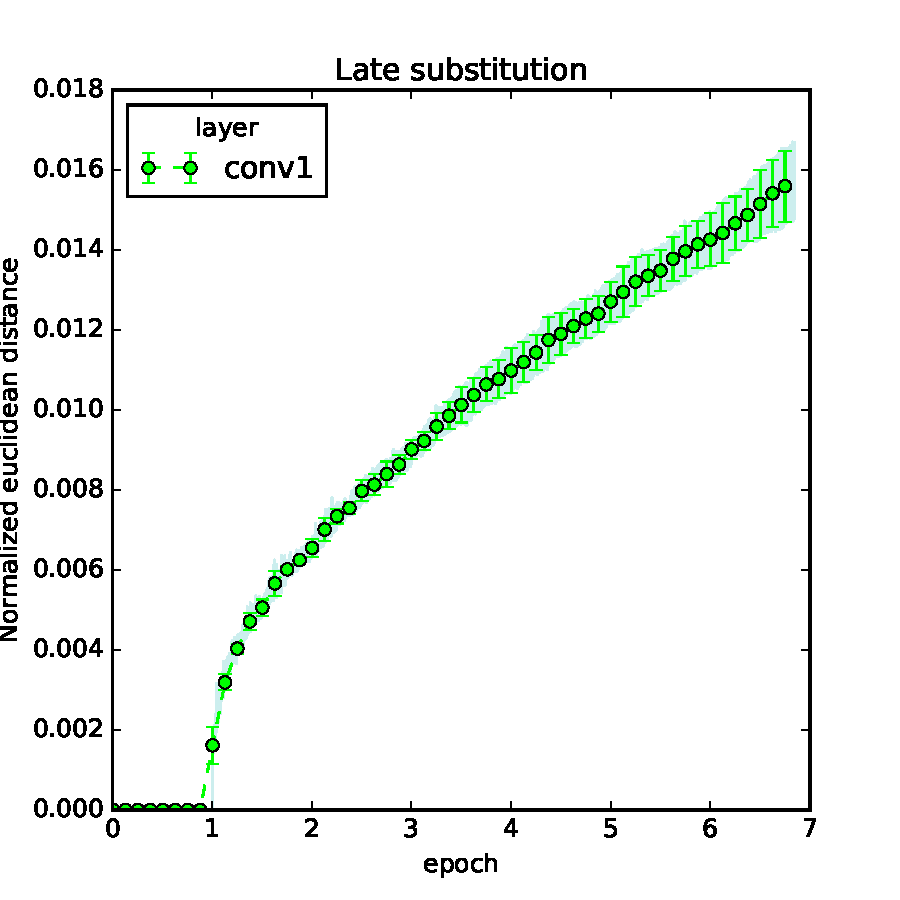
\includegraphics[width=0.5\textwidth,height=\textheight]{assets/imagenet-cpu-late.pdf}
\caption{Parameter divergence on AlexNet trained on Imagenet. The two
models differ only in a single example.}
\end{figure}

\hypertarget{capacity-of-deep-neural-networks}{%
\subsection{Capacity of deep neural
networks}\label{capacity-of-deep-neural-networks}}

Many researchers have attempted to compute notions like VC-dimension or
Rademacher complexity of neural networks. The earliest work by Baum and
Haussler bounded the VC-dimension of small neural networks and showed
that as long these networks could be optimized well in the
\emph{underparameterized} regime, then the neural networks would
generalize.\footnote{Baum and Haussler, {``What Size Net Gives Valid
  Generalization?''} in \emph{Advances in Neural Information Processing
  Systems}, 1988.} Later, seminal work by Bartlett showed that the size
of the weights was more important than the number of weights in terms of
understanding generalization capabilities of neural networks.\footnote{Bartlett,
  {``The Sample Complexity of Pattern Classification with Neural
  Networks: The Size of the Weights Is More Important Than the Size of
  the Network,''} \emph{IEEE Transactions on Information Theory} 44, no.
  2 (1998): 525--36.} These bounds were later sharpened using Rademacher
compexity arguments.\footnote{Bartlett and Mendelson, {``Rademacher and
  Gaussian Complexities.''}}

\hypertarget{margin-bounds-for-deep-neural-networks}{%
\subsection{Margin bounds for deep neural
networks}\label{margin-bounds-for-deep-neural-networks}}

The margin theory for linear models conceptually extends to neural
networks. The definition of margin is unchanged. It simply quantifies
how close the network is to making an incorrect prediction. What changes
is that for multi-layer neural networks the choice of a suitable norm is
substantially more delicate.

To see why, a little bit of notation is necessary. We consider
multi-layer neural networks specified by a composition of~\(L\) layers.
Each layer is a linear transformation of the input, followed by a
coordinate-wise non-linear map:

\[
\mathrm{Input}\, x
\rightarrow Ax
\rightarrow \sigma (Ax)
\]

The linear transformation has trainable parameters, while the non-linear
map does not. For notational simplicity, we assume we have the same
non-linearity~\(\sigma\) at each layer scaled so that the map is
\(1\)-Lipschitz. For example, the popular coordinate-wise ReLU
\(\max\{x,0\}\) operation satisfies this assumption.

Given~\(L\) weight matrices~\(\mathcal{A} = (A_1,\ldots,A_L)\) let
\(f_\mathcal{A}\colon\mathbb{R}^d\to\mathbb{R}^k\) denote the function
computed by the corresponding network: \[
  f_\mathcal{A}(x) := A_L\sigma(A_{L-1} \cdots \sigma(A_1 x)\cdots))\,.
\] The network output~\(F_\mathcal{A}(x)\in\mathbb{R}^{k}\) is converted
to a class label in~\(\{1,\ldots,k\}\) by taking the~\(\arg\max\) over
components, with an arbitrary rule for breaking ties. We
assume~\(d\ge k\) only for notational convenience.

Our goal now is to define a complexity measure of the neural network
that will allow us to prove a margin bound. Recall that margins are
meaningless without a suitable normalization of the network. Convince
yourself that the Euclidean norm can no longer work for multi-layer ReLU
networks. After all we can scale the linear transformation on one later
by a constant~\(c\) and a subsequent layer by a constant~\(1/c\). Since
the ReLU non-linearity is piecewise linear, this transformation changes
the Euclidean norm of the weights arbitrarily without changing the
function that the network computes.

There's much ongoing work about what good norms are for deep neural
networks. We will introduce one possible choice here.

Let~\(\|\cdot\|_{\mathrm{op}}\) denote the spectral norm. Also, let
\(\|A\|_{2,1}=\left\| (\|{}A_{:,1}\|_2, \ldots, \|{}A_{:,m} \|_2)\right\|_1\)
the matrix norm, where we apply the~\(\ell_2\)-norm to each column of
the matrix and then take the~\(\ell_1\)-norm of the resulting vector.

The \emph{spectral complexity} \(R_\mathcal{A}\) of a
network~\(F_\mathcal{A}\) with weights~\(\mathcal{A}\) is the defined as
\begin{equation}   R_{\mathcal{A}}   :=   \left(\prod_{i=1}^L\|A_i\|_{\mathrm{op}}\right)   \left(\sum_{i=1}^L \left(\frac{ \|A_i^{\top} - M_i^{\top}\|_{2,1}}{\|A_i\|_{\mathrm{op}}}\right)^{2/3}\right)^{3/2}\,.   \label{eq:spec_comp} \end{equation}
Here, the matrices~\(M_1,\dots, M_L\) are free parameters that we can
choose to minimize the bound. Random matrices tend to be good choices.

The following theorem provides a generalization bound for neural
networks with fixed nonlinearities and weight matrices~\(\mathcal{A}\)
of bounded spectral complexity~\(R_{\mathcal{A}}\).

\begin{Theorem}

Given data~\((x_1,y_1),\dots,(x_n,y_n)\) drawn i.i.d. from any
probability distribution over~\(\mathbb{R}^d\times\{1,\ldots,k\}\), with
probability at least \(1-\delta\), for every margin~\(\theta > 0\) and
every network \(f_{\mathcal{A}} \colon \mathbb{R}^d \to \mathbb{R}^k,\)
\begin{align*}     R[f_{\mathcal{A}}]- R_S^{\theta}[f_{\mathcal{A}}]     \leq \widetilde{{\cal O}}     \left( \frac {R_{\mathcal{A}}\sqrt{ \sum_i \|x_i\|_2^2 }\ln(d)}{\theta n} + \sqrt{\frac {\ln(1/\delta)}{n}} \right),    \end{align*}
where
\(R_S^{\theta}[f] \leq n^{-1} \sum_i \mathbf{1}\left[ f(x_i)_{y_i} \leq \theta + \max_{j\neq y_i} f(x_i)_j \right]\).

\end{Theorem}

The proof of the theorem involves Rademacher complexity and so-called
data-dependent covering arguments. Although it can be shown empirically
that the above complexity measure~\(R_{\mathcal{A}}\) is somewhat
correlated with generalization performance in some cases, there is no
reason to believe that it is the ``right'' complexity measure. The bound
has other undesirable properties, such as an exponential dependence on
the depth of the network as well as an implicit dependence on the size
of the network.

\hypertarget{implicit-regularization-by-stochastic-gradient-descent-in-deep-learning}{%
\subsection{Implicit regularization by stochastic gradient descent in
deep
learning}\label{implicit-regularization-by-stochastic-gradient-descent-in-deep-learning}}

There have been recent attempts to understand the dynamics of stochastic
gradient descent on deep neural networks. Using an argument similar to
the one we used to reason about convergence of the \emph{predictions} of
deep neural networks, Jacot et al.~used a differential equations
argument to understand to which \emph{function} stochastic gradient
converged.\footnote{Jacot, Gabriel, and Hongler, {``Neural Tangent
  Kernel.''}}

Here we can sketch the rough details of their argument. Recall our
expression for the dynamics of the predictions in gradient descent: \[
    \hat{y}_{t+1}-y = (I -  \alpha \mathsf{D}(w_t)^T \mathsf{D}(w_t))(\hat{y}_t - y) + \alpha \epsilon_t\,.
\] If~\(\alpha\) is very small, we can further approximate this as \[
    \hat{y}_{t+1}-y = (I -  \alpha \mathsf{D}(w_0)^T \mathsf{D}(w_0))(\hat{y}_t - y) + \alpha \epsilon'_t\,.
\] Now~\(\epsilon'_t\) captures both the curvature of the function
representation and the deviation of the weights from their initial
condition. Note that in this case,~\(\mathsf{D}(w_0)\) is a constant for
all time. The matrix~\(\mathsf{D}(w_0)^T \mathsf{D}(w_0)\)
is~\(n \times n\), positive semidefinite, and only depends on the data
and the initial setting of the weights. When the weights are random,
this is a kernel induced by random features. The expected value of this
random feature embedding is called a \emph{Neural Tangent Kernel}. \[
    k(x_1,x_2) = \mathop\mathbb{E}_{w_0} \left[\langle \nabla_w f(x_1; w_0), \nabla_w f(x_2;w_0)
    \rangle \right] \,.
\]

Using a limit where~\(\alpha\) tends to zero, Jacot et. al argue that a
deep neural net will find a minimum norm solution in the RKHS of the
Neural Tangent Kernel. This argument was made non-asymptotic by Heckel
and Soltanolkotabi.\footnote{Heckel and Soltanolkotabi, {``Compressive
  Sensing with Un-Trained Neural Networks: Gradient Descent Finds the
  Smoothest Approximation,''} 2020.} In the generalization chapter, we
showed that the minimum norm solution of in RKHS generalized with a rate
of~\(O(1/n)\). Hence, this argument suggests a similar rate of
generalization may occur in deep learning, provided the norm of the
minimum norm solution does not grow to rapidly with the number of data
points and that the true function optimized by stochastic gradient
descent isn't too dissimilar from the Neural Tangent Kernel limit. We
note that this argument is qualitative, and there remains work to be
done to make these arguments fully rigorous.

Perhaps the most glaring issue with NTK arguments is that they do not
reflect practice. Models trained with Neural Tangent Kernels do not
match the predictive performance of the corresponding neural network.
Moreover, simpler kernels inspired by these networks can out perform
Neural Tangent Kernels.\footnote{Shankar et al., {``Neural Kernels
  Without Tangents.''}} There is a significant gap between the theory
and practice here, but the research is new and remains active and this
gap may be narrowed in the coming years.

\hypertarget{chapter-notes-6}{%
\section{Chapter notes}\label{chapter-notes-6}}

Deep learning is at this point a vast field with tens of thousands of
papers. We don't attempt to survey or systematize this vast literature.
It's worth emphasizing though the importance of learning about the area
by experimenting with avaialble code on publicly available datasets. The
next chapter will cover datasets and benchmarks in detail.

Apart from the development of benchmark datasets, one of the most
important advances in deep learning over the last decade has been the
development of high quality, open source software. This software makes
it easier than ever to prototype deep neural network models. One such
open source project is Pytorch\footnote{\href{https://pytorch.org/}{pytorch.org}},
which we recommend for the researcher interested in experimenting with
deep neural networks.

The best way to begin to understand some of the nuances of architecture
selection is to find pre-existing code and understand how it is
composed. We recommend the tutorial by David Page which demonstrates how
the many different pieces fit together in a deep learning
pipeline.\footnote{\href{https://myrtle.ai/learn/how-to-train-your-resnet/}{myrtle.ai/learn/how-to-train-your-resnet}}

For the reader interested in a more in depth understanding of automatic
differentiation, we recommend Griewank and Walther's \emph{Evaluating
Derivatives}.\footnote{Griewank and Walther, \emph{Evaluating
  Derivatives: Principles and Techniques of Algorithmic
  Differentiation}, 2nd ed. (SIAM, 2008).} This text works through a
variety of unexpected scenarios---such as implicitly defined
functions---where gradients can be computed algorithmically.
Jax\footnote{\href{https://github.com/google/jax}{github.com/google/jax}}
is open source automatic differentiation package that incorporates many
of these techniques, and is useful for any application that could be
assisted by automatic differentiation.

Residual networks were introduced by He et al.\footnote{He et al.,
  {``Deep Residual Learning for Image Recognition.''}} The observation
about linear residual networks is due to Hardt and Ma.\footnote{Hardt
  and Ma, {``Identity Matters in Deep Learning,''} in
  \emph{International Conference on Learning Representations}, 2017.}

\chapter{Datasets}

It's become commonplace to point out that machine learning models are
only as good as the data they're trained on. The old slogan ``garbage
in, garbage out'' no doubt applies to machine learning practice, as does
the related catchphrase ``bias in, bias out.'' Yet, these aphorisms
still understate---and somewhat misrepresent---the significance of data
for machine learning.

It's not only the output of a learning algorithm that may suffer with
poor input data. A dataset serves many other vital functions in the
machine learning ecosystem. The dataset itself is an integral part of
the problem formulation. It implicitly sorts out and operationalizes
what the problem is that practitioners end up solving. Datasets have
also shaped the course of entire scientific communities in their
capacity to measure and benchmark progress, support competitions, and
interface between researchers in academia and practitioners in industry.

If so much hinges on data in machine learning, it might come as a
surprise that there is no simple answer to the question of what makes
data good for what purpose. The collection of data for machine learning
applications has not followed any established theoretical framework,
certainly not one that was recognized a priori.

In this chapter, we take a closer look at popular datasets in the field
of machine learning and the benchmarks that they support. We trace out
the history of benchmarks and work out the implicit scientific
methodology behind machine learning benchmarks.

We limit the scope of this chapter in some important ways. Our focus
will be largely on publicly available datasets that support training and
testing purposes in machine learning research and applications.
Primarily, we critically examine the train-and-test paradigm machine
learning practitioners take for granted today.

\hypertarget{the-scientific-basis-of-machine-learning-benchmarks}{%
\section{The scientific basis of machine learning
benchmarks}\label{the-scientific-basis-of-machine-learning-benchmarks}}

Methodologically, much of modern machine learning practice rests on a
variant of \emph{trial and error}, which we call the \emph{train-test
paradigm}. Practitioners repeatedly build models using any number of
heuristics and test their performance to see what works. Anything goes
as far as training is concerned, subject only to computational
constraints, so long as the performance looks good in testing. Trial and
error is sound so long as the testing protocol is robust enough to
absorb the pressure placed on it. We will examine to which extent this
is the case in machine learning.

From a theoretical perspective, the best way to test the performance of
a classifier~\(f\) is to collect a sufficiently large fresh
dataset~\(S\) and to compute the empirical risk~\(R_S[f]\). We already
learned that the empirical risk in this case is an unbiased estimate of
the risk of the classifier. For a bounded loss function and a test set
of size~\(n\), an appeal to Hoeffding's inequality proves the
generalization gap to be no worse than~\(O(1/\sqrt{n})\). We can go a
step further and observe that if we take union bound over~\(k\) fixed
classifiers, our fresh sample will simultaneously provide good estimates
for all~\(k\) classifiers up to a maximum error
of~\(O(\sqrt{\log(k)/n})\). In fact, we can apply any of the
mathematical tools we saw in the Generalization chapter so long as the
sample~\(S\) really is a fresh sample with respect to the set of models
we want to evaluate.

Data collection, however, is a difficult and costly task. In most
applications, practitioners cannot sample fresh data for each model they
would like to try out. A different practice has therefore become the
de-facto standard. Practitioners split their dataset into typically two
parts, a \emph{training set} used for training a model, and a \emph{test
set} used for evaluating its performance.\footnote{Sometimes
  practitioners divide their data into multiple splits, e.g., training,
  validation, and test sets. However, for our discussion here that won't
  be necessary.} Often the split is determined when the dataset is
created. Datasets used for benchmarks in particular have one fixed split
persistent throughout time. A number of variations on this theme go
under the name \emph{holdout method}.\index{holdout method}

Machine learning competitions have adopted the same format. The company
Kaggle, for example, has organized hundreds of competitions since it was
founded. In a competition, a holdout set is kept secret and is used to
rank participants on a public leaderboard as the competition unfolds. In
the end, the final winner is whoever scores highest on a separate secret
test set not used to that point.\index{Kaggle}\index{competition}

In all applications of the holdout method the hope is that the test set
will serve as a fresh sample that provides good risk estimates for all
the models. The central problem is that practitioners don't just use the
test data once only to retire it immediately thereafter. The test data
are used incrementally for building one model at a time while
incorporating feedback received previously from the test data. This
leads to the fear that eventually models begin to \emph{overfit} to the
test data.\index{overfit}

Duda and Hart summarize the problem aptly in their 1973
textbook:\footnote{Duda, Hart, and Stork, \emph{Pattern Classification
  and Scene Analysis}, vol. 3 (Wiley New York, 1973).}

\begin{quote}
In the early work on pattern recognition, when experiments were often
done with very small numbers of samples, the same data were often used
for designing and testing the classifier. This mistake is frequently
referred to as ``testing on the training data.'' A related but less
obvious problem arises when a classifier undergoes a long series of
refinements guided by the results of repeated testing on the same data.
This form of ``training on the testing data'' often escapes attention
until new test samples are obtained.
\end{quote}

Nearly half a century later, Hastie, Tibshirani, and Friedman still
caution in the 2017 edition of their influential textbook:\footnote{Hastie,
  Tibshirani, and Friedman, \emph{The Elements of Statistical Learning:
  Data Mining, Inference, and Prediction (Corrected 12th Printing)}
  (Springer, 2017).}

\begin{quote}
Ideally, the test set should be kept in a ``vault,'' and be brought out
only at the end of the data analysis. Suppose instead that we use the
test-set repeatedly, choosing the model with smallest test-set error.
Then the test set error of the final chosen model will underestimate the
true test error, sometimes substantially.
\end{quote}

Indeed, reuse of test data---on the face of it---invalidates the
statistical guarantees of the holdout method. The classifiers created
with knowledge about prior test-set evaluations are no longer
independent of the test data. In other words, the sample isn't fresh
anymore. While the suggestion to keep the test data in a ``vault'' is
safe, it couldn't be further from the reality of modern practice. We
will soon see that popular test datasets often see tens of thousands of
evaluations in a single research paper.

We could try to salvage the situation by relying on uniform convergence.
If all models we try out have sufficiently small complexity in some
formal sense, such as VC-dimension, we could use the tools from the
Generalization chapter to negotiate some sort of a bound. However, the
whole point of the train-test paradigm is not to constrain the
complexity of the models a priori, but rather to let the practitioner
experiment freely. Moreover, if we had an actionable theoretical
generalization guarantee to begin with, there would hardly be any need
for the holdout method whose purpose is to provide an empirical estimate
where theoretical guarantees are lacking.

Before we discuss the ``training on the testing data'' problem any
further, it's helpful to get a better sense of concrete machine learning
benchmarks, their histories, and their impact within the community.

\hypertarget{a-tour-of-datasets-in-different-domains}{%
\section{A tour of datasets in different
domains}\label{a-tour-of-datasets-in-different-domains}}

The creation of datasets in machine learning does not follow a clear
theoretical framework. Datasets aren't collected to test a specific
scientific hypothesis. In fact, we will see that there are many
different roles data plays in machine learning. As a result, it makes
sense to start by looking at a few influential datasets from different
domains to get a better feeling for what they are, what motivated their
creation, how they organized communities, and what impact they had.

\hypertarget{timit}{%
\subsection{TIMIT}\label{timit}}

Automatic speech recognition is a machine learning problem of
significant commercial interest. Its roots date back to the early 20th
century.\footnote{Li and Mills, {``Vocal Features: From Voice
  Identification to Speech Recognition by Machine,''} \emph{Technology
  and Culture} 60, no. 2 (2019): S129--60.}

Interestingly, speech recognition also features one of the oldest
benchmarks data sets, the TIMIT (Texas Instruments/Massachusetts
Institute for Technology) data. The creation of the dataset was funded
through a 1986 DARPA program on speech recognition. In the mid-eighties,
artificial intelligence was in the middle of a ``funding winter'' where
many governmental and industrial agencies were hesitant to sponsor AI
research because it often promised more than it could deliver. DARPA
program manager Charles Wayne proposed a way around this problem was
establishing more rigorous evaluation methods. Wayne enlisted the
National Institute of Standards and Technology to create and curate
shared datasets for speech, and he graded success in his program based
on performance on recognition tasks on these data sets.

Many now credit Wayne's program with kick starting a revolution of
progress in speech recognition.\footnote{{``Obituary: {F}red
  {J}elinek,''} \emph{Computational Linguistics} 36, no. 4 (2010):
  595--99; Church, {``Emerging Trends''}; Liberman and Wayne, {``Human
  Language Technology.''}} According to Church,

\begin{quote}
It enabled funding to start because the project was
glamour-and-deceit-proof, and to continue because funders could measure
progress over time. Wayne's idea makes it easy to produce plots which
help sell the research program to potential sponsors. A less obvious
benefit of Wayne's idea is that it enabled hill climbing. Researchers
who had initially objected to being tested twice a year began to
evaluate themselves every hour.
\end{quote}

A first prototype of the TIMIT dataset was released in December of 1988
on a CD-ROM. An improved release followed in October 1990. TIMIT already
featured the training/test split typical for modern machine learning
benchmarks. There's a fair bit we know about the creation of the data
due to its thorough documentation.\footnote{Garofolo et al., {``DARPA
  {TIMIT} Acoustic-Phonetic Continous Speech Corpus {CD-ROM}. {NIST}
  Speech Disc 1-1.1,''} \emph{STIN} 93 (1993): 27403.}

TIMIT features a total of about 5 hours of speech, composed of 6300
utterances, specifically, 10 sentences spoken by each of 630 speakers.
The sentences were drawn from a corpus of 2342 sentences such as the
following.\index{TIMIT}

\begin{verbatim}
She had your dark suit in greasy wash water all year. (sa1)
Don't ask me to carry an oily rag like that. (sa2)
This was easy for us. (sx3)
Jane may earn more money by working hard. (sx4)
She is thinner than I am. (sx5)
Bright sunshine shimmers on the ocean. (sx6)
Nothing is as offensive as innocence. (sx7)
\end{verbatim}

The TIMIT documentation distinguishes between 8 major dialect
regions\footnote{New England, Northern, North Midland, South Midland,
  Southern, New York City, Western, Army Brat (moved around)} in the
United States. Of the speakers, 70\% are male and 30\% are female. All
native speakers of American English, the subjects were primarily
employees of Texas Instruments at the time. Many of them were new to the
Dallas area where they worked.

Racial information was supplied with the distribution of the data and
coded as ``White,'' ``Black,'' ``American Indian,''
``Spanish-American,'' ``Oriental,'' and ``Unknown.'' Of the 630
speakers, 578 were identified as White, 26 as Black, 2 as American
Indian, 2 as Spanish-American, 3 as Oriental, and 17 as unknown.

\begin{longtable}[]{@{}llll@{}}
\caption{Demographic information about the TIMIT
speakers}\tabularnewline
\toprule
& Male & Female & Total (\%) \\
\midrule
\endfirsthead
\toprule
& Male & Female & Total (\%) \\
\midrule
\endhead
White & 402 & 176 & 578 (91.7\%) \\
Black & 15 & 11 & 26 (4.1\%) \\
American Indian & 2 & 0 & 2 (0.3\%) \\
Spanish-American & 2 & 0 & 2 (0.3\%) \\
Oriental & 3 & 0 & 3 (0.5\%) \\
Unknown & 12 & 5 & 17 (2.6\%) \\
\bottomrule
\end{longtable}

The documentation notes:

\begin{quote}
In addition to these 630 speakers, a small number of speakers with
foreign accents or other extreme speech and/or hearing abnormalities
were recorded as ``auxiliary'' subjects, but they are not included on
the CD-ROM.
\end{quote}

It comes to no surprise that early speech recognition models had
significant demographic and racial biases in their performance.

Today, several major companies, including Amazon, Apple, Google, and
Microsoft, all use speech recognition models in a variety of products
from cell phone apps to voice assistants. Today, speech recognition
lacks a major open benchmark that would support the training models
competitive with the industrial counterparts. Industrial speech
recognition pipelines are often complex systems that use proprietary
data sources that not a lot is known about. Nevertheless, even today's
speech recognition systems continue to have racial biases.\footnote{Koenecke
  et al., {``Racial Disparities in Automated Speech Recognition,''}
  \emph{Proceedings of the National Academy of Sciences} 117, no. 14
  (2020): 7684--89.}

\hypertarget{uci-machine-learning-repository}{%
\subsection{UCI Machine Learning
Repository}\label{uci-machine-learning-repository}}

The UCI Machine Learning Repository currently hosts more than 500
datasets, mostly for different classification and regression tasks. Most
datasets are relatively small, many of them structured tabular data sets
with few attributes.\index{UCI}

The UCI Machine Learning Repository contributed to the adoption of the
train-test paradigm in machine learning in the late 1980s. Langley
recalls:

\begin{quote}
The experimental movement was aided by another development. David Aha,
then a PhD student at UCI, began to collect data sets for use in
empirical studies of machine learning. This grew into the UCI Machine
Learning Repository (http://archive.ics.uci.edu/ml/), which he made
available to the community by FTP in 1987. This was rapidly adopted by
many researchers because it was easy to use and because it let them
compare their results to previous findings on the same tasks.\footnote{Langley,
  {``The Changing Science of Machine Learning.''}}
\end{quote}

Aha's PhD work involved evaluating nearest-neighbor methods, and he
wanted to be able to compare the utility of his algorithms to decision
tree induction algorithms, popularized by Ross Quinlan. Aha describes
his motivation for building the UCI repository as follows.

\begin{quote}
I was determined to create and share it, both because I wanted to use
the datasets for my own research and because I thought it was ridiculous
that the community hadn't fielded what should have been a useful
service. I chose to use the simple attribute-value representation that
Ross Quinlan was using so successfully for distribution with his TDIDT
implementations.\footnote{David Aha. Personal communication.}
\end{quote}

The UCI dataset was wildly successful, and partially responsible for the
renewed interest in pattern recognition methods in machine learning.
However, this success came with some detractors. By the mid 1990s, many
were worried that evaluation-by-benchmark encouraged chasing
state-of-the-art results and writing incremental papers. Aha reflects:

\begin{quote}
By ICML-95, the problems ``caused'' by the repository had become
popularly espoused. For example, at that conference Lorenza Saitta had,
in an invited workshop that I co-organized, passionately decried how it
allowed researchers to publish dull papers that proposed small
variations of existing supervised learning algorithms and reported their
small-but-significant incremental performance improvements in comparison
studies.
\end{quote}

Nonetheless, the UCI repository remains one of the most popular source
for benchmark data sets in machine learning, and many of the early data
sets still are used for benchmarking in machine learning research. The
most popular dataset in the UCI repository is Ronald A. Fisher's Iris
Data Set that Fisher collected for his 1936 paper on ``The use of
multiple measurements in taxonomic problems.''

The second most popular dataset in the UCI repository\footnote{As of
  October, 2020.} is the \emph{Adult} dataset. Extracted from the 1994
Census database, the dataset features nearly 50,000 instances describing
individual in the United States, each having 14 attributes. The goal is
to classify whether an individual earns more than 50,000 US dollars or
less.

The Adult dataset became popular in the algorithmic fairness community,
largely because it is one of the few publicly available datasets that
features demographic information including \emph{gender} (coded in
binary as male/female), as well as \emph{race} (coded as
Amer-Indian-Eskimo, Asian-Pac-Islander, Black, Other, and White).

Unfortunately, the data has some idiosyncrasies that make it less than
ideal for understanding biases in machine learning models. Due to the
age of the data, and the income cutoff at \$50,000, almost all instances
labeled \emph{Black} are below the cutoff, as are almost all instances
labeled \emph{female}. Indeed, a standard logistic regression model
trained on the data achieves about 85\% accuracy overall, while the same
model achieves 91\% accuracy on Black instances, and nearly 93\%
accuracy on female instances. Likewise, the ROC curves for the latter
two groups enclose actually more area than the ROC curve for male
instances. This is a rather untypical situation since often machine
learning models perform more poorly on historically disadvantaged
groups.

\hypertarget{mnist}{%
\subsection{MNIST}\label{mnist}}

The MNIST dataset contains images of handwritten digits. Its most common
version has 60,000 training images and 10,000 test images, each having
28x28 black and white pixels.\index{MNIST}

\begin{figure}
\centering
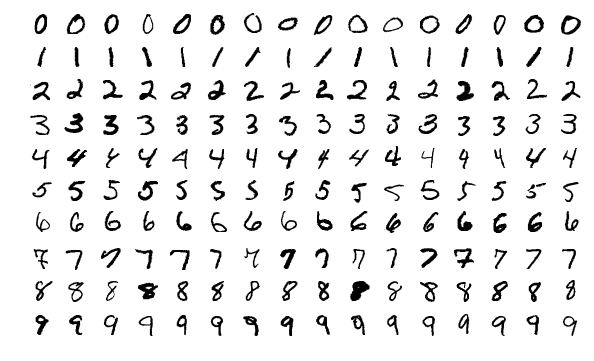
\includegraphics{assets/datasets_mnist-examples.png}
\caption{A sample of MNIST digits}
\end{figure}

MNIST was created by researchers Burges, Cortes, and Lecun from data by
the National Institute of Standards and Technology (NIST). The dataset
was introduced in a research paper in 1998 to showcase the use of
gradient-based deep learning methods for document recognition
tasks.\footnote{LeCun et al., {``Gradient-Based Learning Applied to
  Document Recognition,''} \emph{Proceedings of the IEEE} 86, no. 11
  (1998): 2278--2324.} However, the authors released the data set to
provide a convenient benchmark of image data, in contrast to UCI's
predominantly tabular data. The MNIST website states

\begin{quote}
It is a good database for people who want to try learning techniques and
pattern recognition methods on real-world data while spending minimal
efforts on preprocessing and formatting.\footnote{http://yann.lecun.com/exdb/mnist/}
\end{quote}

MNIST became a highly influential benchmark in the machine learning
community. Two decades and over 30,000 citation later, researchers
continue to use the data actively.

The original NIST data had the property that training and test data came
from two different populations. The former featured the handwriting of
two thousand American Census Bureau employees, whereas the latter came
from five hundred American high school students.\footnote{Grother,
  {``NIST Special Database 19 Handprinted Forms and Characters
  Database,''} \emph{National Institute of Standards and Technology},
  1995.} The creators of MNIST reshuffled these two data sources and
split them into training and test set. Moreover, they scaled and
centered the digits. The exact procedure to derive MNIST from NIST was
lost, but recently reconstructed by matching images from both data
sources.\footnote{Yadav and Bottou, {``Cold Case: The Lost Mnist
  Digits,''} in \emph{Advances in Neural Information Processing
  Systems}, 2019, 13443--52.}\index{NIST}

The original MNIST test set was of the same size as the training set,
but the smaller test set became standard in research use. The 50,000
digits in the original test set that didn't make it into the smaller
test set were later identified and dubbed \emph{the lost
digits}.\footnote{Yadav and Bottou.}

From the beginning, MNIST was intended to be a benchmark used to compare
the strengths of different methods. For several years, LeCun maintained
an informal leaderboard on a personal website that listed the best
accuracy numbers that different learning algorithms achieved on
MNIST.\index{leaderboard}

\begin{longtable}[]{@{}ll@{}}
\caption{A snapshot of the original MNIST leaderboard from February 2,
1999. Source: Internet Archive (Retrieved: December 4,
2020)}\tabularnewline
\toprule
Method & Test error (\%) \\
\midrule
\endfirsthead
\toprule
Method & Test error (\%) \\
\midrule
\endhead
linear classifier (1-layer NN) & 12.0 \\
linear classifier (1-layer NN) {[}deskewing{]} & 8.4 \\
pairwise linear classifier & 7.6 \\
K-nearest-neighbors, Euclidean & 5.0 \\
K-nearest-neighbors, Euclidean, deskewed & 2.4 \\
40 PCA + quadratic classifier & 3.3 \\
1000 RBF + linear classifier & 3.6 \\
K-NN, Tangent Distance, 16x16 & 1.1 \\
SVM deg 4 polynomial & 1.1 \\
Reduced Set SVM deg 5 polynomial & 1.0 \\
Virtual SVM deg 9 poly {[}distortions{]} & 0.8 \\
2-layer NN, 300 hidden units & 4.7 \\
2-layer NN, 300 HU, {[}distortions{]} & 3.6 \\
2-layer NN, 300 HU, {[}deskewing{]} & 1.6 \\
2-layer NN, 1000 hidden units & 4.5 \\
2-layer NN, 1000 HU, {[}distortions{]} & 3.8 \\
3-layer NN, 300+100 hidden units & 3.05 \\
3-layer NN, 300+100 HU {[}distortions{]} & 2.5 \\
3-layer NN, 500+150 hidden units & 2.95 \\
3-layer NN, 500+150 HU {[}distortions{]} & 2.45 \\
LeNet-1 {[}with 16x16 input{]} & 1.7 \\
LeNet-4 & 1.1 \\
LeNet-4 with K-NN instead of last layer & 1.1 \\
LeNet-4 with local learning instead of ll & 1.1 \\
LeNet-5, {[}no distortions{]} & 0.95 \\
LeNet-5, {[}huge distortions{]} & 0.85 \\
LeNet-5, {[}distortions{]} & 0.8 \\
Boosted LeNet-4, {[}distortions{]} & 0.7 \\
\bottomrule
\end{longtable}

In its capacity as a benchmark, it became a showcase for the emerging
kernel methods of the early 2000s that temporarily achieved top
performance on MNIST.\footnote{Decoste and Schölkopf, {``Training
  Invariant Support Vector Machines.''}} Today, it is not difficult to
achieve less than 0.5\% classification error with a wide range of
convolutional neural network architectures. The best models classify all
but a few pathological test instances correctly. As a result, MNIST is
widely considered \emph{too easy} for today's research tasks.

MNIST wasn't the first dataset of handwritten digits in use for machine
learning research. Earlier, the US Postal Service (USPS) had released a
dataset of 9298 images (7291 for training, and 2007 for testing). The
USPS data was actually a fair bit harder to classify than MNIST. A
non-negligible fraction of the USPS digits look unrecognizable to
humans,\footnote{Bromley and Sackinger, {``Neural-Network and
  k-Nearest-Neighbor Classifiers,''} \emph{Rapport Technique}, 1991,
  11359--910819.} whereas humans recognize essentially all digits in
MNIST.

\hypertarget{imagenet}{%
\subsection{ImageNet}\label{imagenet}}

ImageNet is a large repository of labeled images that has been highly
influential in computer vision research over the last decade. The image
labels correspond to nouns from the WordNet lexical database of the
English language. WordNet groups nouns into cognitive synonyms, called
\emph{synsets}. The words \emph{car} and \emph{automobile}, for example,
would fall into the same synset. On top of these categories WordNet
provides a hierarchical tree structure according to a super-subordinate
relationship between synsets. The synset for \emph{chair}, for example,
is a child of the synset for \emph{furniture} in the wordnet hierarchy.
WordNet existed before ImageNet and in part inspired the creation of
Imagenet.\index{ImageNet}\index{WordNet}

The initial release of ImageNet included about 5000 image categories
each corresponding to a synset in WordNet. These ImageNet categories
averaged about 600 images per category.\footnote{Deng et al.,
  {``Imagenet: A Large-Scale Hierarchical Image Database,''} in
  \emph{Computer Vision and Pattern Recognition}, 2009, 248--55.}
ImageNet grew over time and its Fall 2011 release had reached about
32,000 categories.

The construction of ImageNet required two essential steps:

\begin{enumerate}
\def\labelenumi{\arabic{enumi}.}
\tightlist
\item
  The first was the retrieval of candidate images for each synset.
\item
  The second step in the creation process was the labeling of images.
\end{enumerate}

Scale was an important consideration due to the target size of the image
repository.

This first step utilized available image databases with a search
interface, specifically, Flickr. Candidate images were taken from the
image search results associated with the synset nouns for each category.

For the second labeling step, the creators of ImageNet turned to
Amazon's Mechanical Turk platform (MTurk). MTurk is an online labor
market that allows individuals and corporations to hire on-demand
workers to perform simple tasks. In this case, MTurk workers were
presented with candidate images and had to decide whether or not the
candidate image was indeed an image corresponding to the category that
it was putatively associated with.\index{MTurk}

It is important to distinguish between this ImageNet database and a
popular machine learning benchmark and competition, called ImageNet
Large Scale Visual Recognition Challenge (ILSVRC), that was derived from
it.\footnote{Russakovsky et al., {``Imagenet Large Scale Visual
  Recognition Challenge,''} \emph{International Journal of Computer
  Vision} 115, no. 3 (2015): 211--52.} The competition was organized
yearly from 2010 until 2017 to ``measure the progress of computer vision
for large scale image indexing for retrieval and
annotation.\index{ILSVRC}'' In 2012, ILSVRC reached significant
notoriety in both industry and academia when a deep neural network
trained by Krizhevsky, Sutskever, and Hinton outperformed all other
models by a significant margin.\footnote{Krizhevsky, Sutskever, and
  Hinton, {``ImageNet Classification with Deep Convolutional Neural
  Networks.''}} This result---yet again an evaluation in a train-test
paradigm---helped usher in the latest era of exuberant interest in
machine learning and neural network models under the rebranding as
\emph{deep learning}.\footnote{Malik, {``What Led Computer Vision to
  Deep Learning?''} \emph{Communications of the {ACM}} 60, no. 6 (2017):
  82--83.}

When machine learning practitioners say ``ImageNet'' they typically
refer to the data used for the image classification task in the 2012
ILSVRC benchmark. The competition included other tasks, such as object
recognition, but image classification has become the most popular task
for the dataset. Expressions such as ``a model trained on ImageNet''
typically refer to training an image classification model on the
benchmark data set from 2012.

Another common practice involving the ILSVRC data is
\emph{pre-training}. Often a practitioner has a specific classification
problem in mind whose label set differs from the 1000 classes present in
the data. It's possible nonetheless to use the data to create useful
features that can then be used in the target classification problem.
Where ILSVRC enters real-world applications it's often to support
pre-training.\index{pre-training}

This colloquial use of the word ImageNet can lead to some confusion, not
least because the ILSVRC-2012 dataset differs significantly from the
broader database. It only includes a subset of 1000 categories.
Moreover, these categories are a rather skewed subset of the broader
ImageNet hierarchy. For example, of these 1000 categories only three are
in the \emph{person} branch of the WordNet hierarchy, specifically,
\emph{groom}, \emph{baseball player}, and \emph{scuba diver}. Yet, more
than 100 of the 1000 categories correspond to different dog
breeds.\footnote{The number is 118, to be exact, not counting wolves,
  foxes, and wild dogs that are also present among the 1000 categories.}

What motivated the exact choice of these 1000 categories is not entirely
clear. The apparent canine inclination, however, isn't just a quirk
either. At the time, there was an interest in the computer vision
community in making progress on prediction with many classes, some of
which are very similar. This reflects a broader pattern in the machine
learning community. The creation of datasets is often driven by an
intuitive sense of what the technical challenges are for the field. In
the case of ImageNet, \emph{scale}, both in terms of the number of data
points as well as the number of classes, was an important motivation.

The large scale annotation and labeling of datasets, such as we saw in
the case of Imagenet, fall into a category of labor that anthropologist
Gray and computer scientist Suri coined \emph{Ghost Work} in their book
of the same name.\footnote{Gray and Suri, \emph{Ghost Work: How to Stop
  Silicon Valley from Building a New Global Underclass} (Eamon Dolan
  Books, 2019).} They point out:

\begin{quote}
MTurk workers are the AI revolution's unsung heroes.
\end{quote}

Indeed, ImageNet was labeled by about 49,000 MTurk workers from 167
countries over the course of multiple years.

\hypertarget{longevity-of-benchmarks}{%
\section{Longevity of benchmarks}\label{longevity-of-benchmarks}}

The holdout method is central to the scientific and industrial
activities of the machine learning community. Thousands of research
papers have been written that report numbers on popular benchmark data,
such as, MNIST, CIFAR-10, or Imagenet. Often extensive tuning and
hyperparameter optimization went into each such research project to
arrive at the final accuracy numbers reported in the paper.

Does this extensive reuse of test sets not amount to what Duda and Hart
call the ``training on the testing data'' problem? If so, how much of
the progress that has been made is real, and how much amounts of
overfitting to the test data?

To answer these questions we will develop some more theory that will
help us interpret the outcome of empirical meta studies into the
longevity of machine learning benchmarks.

\hypertarget{the-problem-of-adaptivity}{%
\subsection{The problem of adaptivity}\label{the-problem-of-adaptivity}}

Model building is an iterative process where the performance of a model
informs subsequent design choices. This iterative process creates a
closed feedback loop between the analyst and the test set. In
particular, the classifiers the analyst chooses are not independent of
the test set, but rather
\emph{adaptive}.\index{adaptive}\index{adaptivity}

Adaptivity can be interpreted as a form of overparameterization. In an
adaptively chosen sequence of classifiers~\(f_1,\dots,f_k,\)
the~\(k\)-th classifier had the ability to incorporate at least~\(k-1\)
bits of information about the performance of previously chosen
classifiers. This suggests that as~\(k\ge n,\) the statistical
guarantees of the holdout method become vacuous. This intuition is
formally correct, as we will see.

To reason about adaptivity, it is helpful to frame the problem as an
interaction between two parties. One party holds the dataset~\(S\).
Think of this party as implementing the holdout method. The other party,
we call \emph{analyst}, can \emph{query} the dataset by requesting the
empirical risk \(R_S[f]\) of a given classifier~\(f\) on the
dataset~\(S\). The parties interact for some number~\(k\) of rounds,
thus creating a sequence of adaptively chosen
classifiers~\(f_1,\dots,f_k.\) Keep in mind that this sequence depends
on the data set! In particular, when~\(S\) is drawn at
random,~\(f_2,\dots, f_k\) become random variables, too, that are in
general not independent of each
other.\index{analyst}\index{adaptive!analyst}

\begin{figure}
\centering
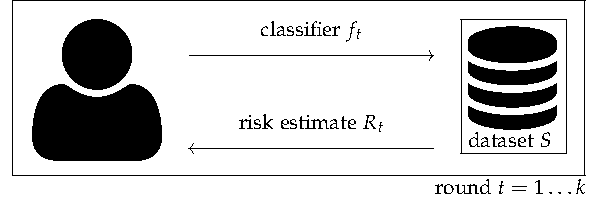
\includegraphics[width=1\textwidth,height=\textheight]{assets/datasets-adaptiveanalyst}
\caption{The adaptive analyst model. The risk estimate need not equal
the empirical risk.}
\end{figure}

In this chapter, we restrict our attention to the case of the zero-one
loss and binary prediction, although the theory extends to other
settings.

Indeed, there is a fairly natural sequence of~\(k\) adaptively chosen
classifiers, resembling the practice of ensembling, on which the
empirical risk is off by at least~\(\Omega(\sqrt{k/n}).\) We present the
idea for the zero-one loss in a binary prediction
problem.\index{ensembling}

\begin{Algorithm}

\textbf{Overfitting by ensembling:}

\begin{enumerate}
\def\labelenumi{\arabic{enumi}.}
\tightlist
\item
  Choose \(k\) of random binary classifiers \(f_1,\dots, f_k.\)
\item
  Compute the set \(I=\{i\in[k]\colon R_S[f_i] < 1/2\}.\)
\item
  Output the classifier \(f=\mathrm{majority}\{ f_i \colon i\in I \}\)
  that takes a majority vote over all the classifiers computed in the
  second step.
\end{enumerate}

\end{Algorithm}

The key idea of the algorithm is to select all the classifiers that have
accuracy strictly better than random guessing. This selection step
creates a bias that gives each selected classifier an advantage over
random guessing. The majority vote in the third step amplifies this
initial advantage into a larger advantage that grows with~\(k\). The
next proposition confirms that indeed this strategy find a classifier
whose empirical risk is bounded a away from~\(1/2\) (random guessing) by
a margin of~\(\Omega(\sqrt{k/n}).\) Since the classifier does nothing
but taking a majority vote over random functions, its population risk is
of course no better than~\(1/2\).

\begin{Proposition}

For sufficiently large~\(k\le n\), overfitting by ensembling returns a
classifier~\(f\) whose classification error satisfies with probability
\(1/3\), \[
R_S[f]\le \frac12-\Omega(\sqrt{k/n})\,.
\] In particular,~\(\Delta_{\mathrm{gen}}(f)\ge\Omega(\sqrt{k/n})\).

\end{Proposition}

We also have a nearly matching upper bound that essentially follows from
a Hoeffding's concentration inequality just as the cardinality bound in
the previous chapter. However, in order to apply Hoeffding's inequality
we first need to understand a useful idea about how we can analyze the
adaptive setting.

The idea is that we can think of the interaction between a fixed analyst
\(\mathcal{A}\) and the data set as a \emph{tree}. The root node is
labeled by \(f_1=\mathcal{A}(\emptyset)\), i.e., the first function that
the analyst queries without any input. The response~\(R_S[f_1]\) takes
on~\(n+1\) possible values. This is because we consider the zero-one
loss, which can only take the values~\(\{0, 1/n, 2/n,\dots, 1\}\). Each
possible response value \(a_1\) creates a new child node in the tree
corresponding to the function \(f_2=\mathcal{A}(a_1)\) that the analyst
queries upon receiving answer~\(a_1\) to the first query~\(f_1\). We
recursively continue the process until we built up a tree of depth~\(k\)
and degree~\(n+1\) at each node.

\begin{figure}
\centering
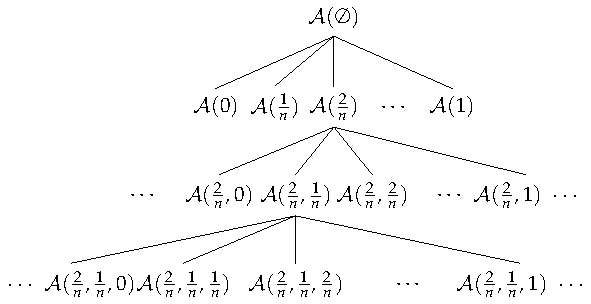
\includegraphics[width=1\textwidth,height=\textheight]{assets/datasets-adaptivetree}
\caption{Constructing a tree of depth \(k\) and degree \(n+1\) given an
adaptive analyst. Each node corresponds to the classifier the analyst
chooses based on the responses seen so far.}
\end{figure}

Note that this tree only depends on the analyst and how it responds to
possible query answers, but it does not depend on the actual query
answers we get out of the sample~\(S\). The tree is therefore
data-independent. This argument is useful in proving the following
proposition.\index{adaptive!tree}

\begin{Proposition}

For any sequence of~\(k\) adaptively chosen
classifiers~\(f_1,\dots, f_k\), the holdout method satisfies with
probability~\(2/3\), \[
\max_{1\le t\le k} \Delta_{\mathrm{gen}}(f_t) \le O\left(\sqrt{k\log(n+1)/n}\right)\,.
\]

\end{Proposition}

\begin{Proof}

The adaptive analyst defines a tree of depth~\(k\) and degree~\(n+1\).
Let \(F\) be the set of functions appearing at any of the nodes in the
tree. Note that~\(|F|\le (n+1)^k.\)

Since this set of functions is data independent, we can apply the
cardinality bound from the previous chapter to argue that the maximum
generalization gap for any function in~\(F\) is bounded by
\(O(\sqrt{\log|F|/n})\) with any constant probability. But the functions
\(f_1,\dots, f_k\) are contained in~\(F\) by construction. Hence, the
claim follows.

\end{Proof}

These propositions show that the principal concern of ``training on the
testing data'' is not unfounded. In the worst case, holdout data can
lose its guarantees rather quickly. If this pessimistic bound manifested
in practice, popular benchmark data sets would quickly become useless.
But does it?

\hypertarget{replication-efforts}{%
\subsection{Replication efforts}\label{replication-efforts}}

In recent replication efforts, researchers carefully recreated new test
sets for the CIFAR-10 and ImageNet classification benchmarks, created
according to the very same procedure as the original test sets. The
researchers then took a large collection of representative models
proposed over the years and evaluated all of them on the new test sets.
In the case of MNIST, researchers used the \emph{lost digits} as a new
test set, since these digits hadn't been used in almost all of the
research on MNIST.

The results of these studies teach us a couple of important lessons that
we will discuss in turn.

\begin{figure}
\centering
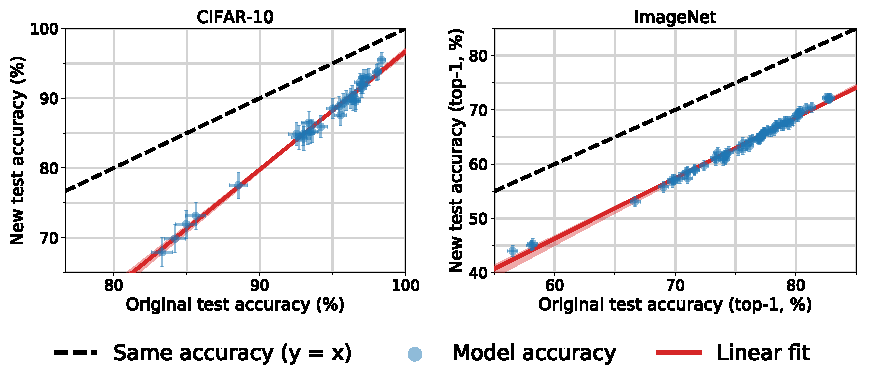
\includegraphics[width=1\textwidth,height=\textheight]{assets/repl-cifar-imagenet}
\caption{Model accuracy on the original test sets vs.~new test sets for
CIFAR-10 and ImageNet. Each data point corresponds to one model in a
test bed of representative models (shown with 95\% Clopper-Pearson
confidence intervals). The plots reveal two main phenomena: (i) There is
generally a significant drop in accuracy from the original to the new
test sets. (ii) The model accuracies closely follow a linear function
with slope greater than 1 (1.7 for CIFAR-10 and 1.1 for ImageNet). This
means that every percentage point of progress on the original test set
translates into more than one percentage point on the new test set. The
two plots are drawn so that their aspect ratio is the same, i.e., the
slopes of the lines are visually comparable. The narrow shaded region is
a 95\% confidence region for the linear fit from 100,000 bootstrap
samples.}
\end{figure}

First, all models suffer a significant drop in performance on the new
test set. The accuracy on the new data is substantially lower than on
the old data. This shows that these models \emph{transfer} surprisingly
poorly from one dataset to a very similar dataset that was constructed
in much the same was as the original data. This observation resonates
with a robust fact about machine learning. Model fitting will do exactly
that. The model will be good on exactly the data it is trained on, but
there is no good reason to believe that it will perform well on other
data. Generalization as we cast it in the preceding chapter is thus
about \emph{interpolation}. It's about doing well on more data from the
same source. It is decidedly \emph{not} about doing well on data from
other sources.

The second observation is relevant to the question of adaptivity; it's a
bit more subtle. The scatter plots admit a clean linear fit with
positive slope. In other words, the better a model is on the old test
set the better it is on the new test set, as well. But notice that newer
models, i.e., those with higher performance on the original test set,
had \emph{more} time to adapt to the test set and to incorporate more
information about it. Nonetheless, the better a model performed on the
old test set the better it performs on the new set. Moreover, on
CIFAR-10 we even see clearly that the absolute performance drops
diminishes with increasing accuracy on the old test set. In particular,
if our goal was to do well on the new test set, seemingly our best
strategy is to continue to inch forward on the old test set. This might
seem counterintuitive.

We will discuss each of these two observations in more detail, starting
with the one about adaptivity.

\hypertarget{benign-adaptivity}{%
\subsection{Benign adaptivity}\label{benign-adaptivity}}

The experiments we just discussed suggest that the effect of adaptivity
was more benign than our previous analysis suggested. This raises the
question what it is that prevents more serious overfitting. There are a
number of pieces to the puzzle that researchers have found. Here we
highlight two.

The main idea behind both mechanisms that damp adaptivity is that the
set of possible nodes in the adaptive tree may be much less than~\(n^k\)
because of empirical conventions. The first mechanism is \emph{model
similarity}. Effectively, model similarity notes that the leaves of the
adaptive tree may be producing similar predictions, and hence the
adaptivity penalty is smaller than our worst case count. The second
mechanism is the \emph{leaderboard principle}. This more subtle effect
states that since publication biases force researchers to chase
state-of-the-art results, they only publish models if they see
significant improvements over prior models.

While we don't believe that these two phenomena explain the entirety of
why overfitting is not observed in practice, they are simple mechanisms
that significantly reduce the effects of adaptivity. As we said, these
are two examples of norms in machine learning practice that diminish the
effects of overfitting.

\hypertarget{model-similarity}{%
\subsection{Model similarity}\label{model-similarity}}

Naively, there are~\(2^n\) total assignments of binary labels to a data
set of size~\(n\). But how many such labeling assignments do we see in
practice? We do not solve pattern recognition problems using the
ensembling attack described above. Rather, we use a relatively small set
of function approximation architectures, and tune the parameters of
these architectures. While we have seen that these architectures can
yield any of the~\(2^n\) labeling patterns, we expect that a much
smaller set of predictions is returned in practice when we run standard
empirical risk minimization.

\emph{Model similarity} formalizes this notion as follows. Given an
adaptively chosen sequence of classifiers~\(f_1,\dots,f_k\), we have a
sequence of estimates of their empirical risks~\(R_1,\dots,R_k\).

\begin{Definition}

We say that a batch of models~\(f_1,\ldots,f_k\)
are~\(\zeta\)-\emph{similar} if for all pairs of models~\(f_i\)
and~\(f_j\) with~\(R_i \leq R_j\), the probability \[
  \mathop\mathbb{P}\left[\{f_j(x) = y\} \cap \{f_i(x) \neq y\} \right] \leq \zeta\,.
\]

\end{Definition}

This definition states that there is low probability of a model with
small empirical risk misclassifying an example where a model with higher
empirical risk was correct. It effectively grades the set of
\emph{examples} as being easier or harder to classify, and suggests that
models with low risk usually get the easy examples correct.

Though simple, this definition has powerful consequences. Mania et
al.\footnote{Mania et al., {``Model Similarity Mitigates Test Set
  Overuse,''} in \emph{Advances in Neural Information Processing
  Systems}, 2019.} showed that this definition was sufficient to reduce
the size of the adaptive tree, and proved that the risk could be bounded
to be at most~\(O(\sqrt{\frac{k^{1-q}}{n}})\) for some positive
scalar~\(q\).The authors also demonstrated empirically on several
benchmarks that deep learning models were~\(\zeta\)-similar. More
recently, Mania and Sra showed that~\(\zeta\)-similarity also implied
the plots observed in our previous section: when empirical risks on two
different test sets are plotted, the scatter of~\((R_i,R_i')\) cluster
around some line.\footnote{Mania and Sra, {``Why Do Classifier
  Accuracies Show Linear Trends Under Distribution Shift?''}
  \emph{arXiv:2012.15483}, 2020.}

\hypertarget{the-leaderboard-principle}{%
\subsection{The leaderboard principle}\label{the-leaderboard-principle}}

The leaderboard principle postulates that \emph{a researcher only cares
if their model improved over the previous best or
not.}\index{leaderboard!principle}\index{leaderboard!error} This
motivates a notion of \emph{leaderboard error} where the holdout method
is only required to track the risk of the best performing model over
time, rather than the risk of all models ever evaluated.

\begin{Definition}

Given an adaptively chosen sequence of classifiers~\(f_1,\dots,f_k,\) we
define the \emph{leaderboard error} of a sequence of estimates
\(R_1,\dots,R_k\) as \[
\mathrm{lberr}(R_1,\dots,R_k)=
\max_{1\le t\le k}\left|\min_{1\le i\le t} R[f_i] - R_t\right|\,.
\]

\end{Definition}

We discuss an algorithm called the Ladder algorithm that achieves small
leaderboard accuracy. The algorithm is simple. For each given
classifier, it compares the empirical risk estimate of the classifier to
the previously smallest empirical risk achieved by any classifier
encountered so far. If the loss is below the previous best by some
margin, it announces the empirical risk of the current classifier and
notes it as the best seen so far. Importantly, if the loss is not
smaller by a margin, the algorithm releases the previous best (rather
than the new loss).

Again, we focus on risk with respect to the zero-one loss, although the
ideas apply more generally.\index{Ladder algorithm}

\begin{Algorithm}

\textbf{Input:} Data set~\(S,\) threshold~\(\eta>0\)

\begin{itemize}
\tightlist
\item
  Assign initial leaderboard error \(R_0\leftarrow 1.\)
\item
  For each round \(t \leftarrow 1,2 \ldots:\)

  \begin{enumerate}
  \def\labelenumi{\arabic{enumi}.}
  \tightlist
  \item
    Receive classifier \(f_t\colon X\to Y\)
  \item
    If \(R_S[f_t] < R_{t-1} - \eta,\) update leaderboard error to
    \(R_t\leftarrow R_S[f_t].\) Else keep previous leaderboard error
    \(R_t\leftarrow R_{t-1}.\)
  \item
    Output leaderboard error \(R_t\)
  \end{enumerate}
\end{itemize}

\end{Algorithm}

The next theorem follows from a variant of the adaptive tree argument we
saw earlier, in which we carefully prune the tree and bound its
size.\index{adaptive!tree}

\begin{Theorem}

For a suitably chosen threshold parameter, for any sequence of
adaptively chosen classifiers~\(f_1,\dots,f_k,\) the Ladder algorithm
achieves with probability~\(1-o(1)\): \[
\mathrm{lberr}(R_1,\dots,R_k)
\le O\left(\frac{\log^{1/3}(kn)}{n^{1/3}}\right)\,.
\]

\end{Theorem}

\begin{Proof}

Set~\(\eta = \log^{1/3}(kn)/n^{1/3}.\) With this setting of~\(\eta,\) it
suffices to show that with probability~\(1-o(1)\) we have for all
\(t\in[k]\) the bound
\(|R_S[f_t]-R[f_t]|\le O(\eta) = O(\log^{1/3}(kn)/n^{1/3})\).

Let~\(\mathcal{A}\) be the adaptive analyst generating the function
sequence. The algorithm~\(\mathcal{A}\) naturally defines a rooted
tree~\(\mathcal{T}\) of depth~\(k\) recursively defined as follows:

\begin{enumerate}
\def\labelenumi{\arabic{enumi}.}
\tightlist
\item
  The root is labeled by \(f_1 = \mathcal{A}(\emptyset).\)
\item
  Each node at depth \(1<i\le k\) corresponds to one realization
  \((h_1,r_1,\dots,h_{i-1},r_{i-1})\) of the tuple of random variables
  \((f_1,R_1,\dots,f_{i-1},R_{i-1})\) and is labeled by
  \(h_i = \mathcal{A}(h_1,r_1,\dots,h_{i-1},r_{i-1}).\) Its children are
  defined by each possible value of the output \(R_i\) of Ladder
  Mechanism on the sequence \(h_1,r_1,\dots,r_{i-1},h_i.\)
\end{enumerate}

Let~\(B = (1/\eta+1)\log(4k(n+1)).\) We claim that the size of the tree
satisfies~\(|\mathcal{T}|\le 2^B.\) To prove the claim, we will uniquely
encode each node in the tree using~\(B\) bits of information. The claim
then follows directly.

The compression argument is as follows. We use
\(\lceil\log k\rceil\le \log(2k)\) bits to specify the depth of the node
in the tree. We then specify the index of each~\(i\in[k]\) for which the
Ladder algorithm performs an ``update'' so that~\(R_i \le R_{i-1}-\eta\)
together with the value~\(R_i.\) Note that since~\(R_i \in[0,1]\) there
can be at most~\(\lceil 1/\eta\rceil\le (1/\eta)+1\) many such steps.
This is because the loss is lower bounded by~\(0\) and decreases
by~\(\eta\) each time there is an update.\footnote{Low bit encoding of
  the adaptive tree. Dashed lines correspond to rounds with no update.
  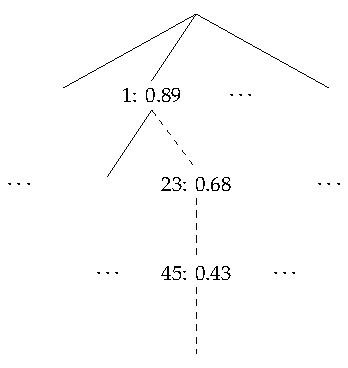
\includegraphics{assets/datasets-ladderpath}}

Moreover, there are at most~\(n+1\) many possible values for~\(R_i\),
since we're talking about the zero-one loss on a dataset of size~\(n\).
Hence, specifying all such indices requires at most
\((1/\eta + 1)(\log(n+1)+\log(2k))\) bits. It is easy that this uniquely
identifies each node in the graph, since for every index~\(i\) not
explicitly listed we know that~\(R_i=R_{i-1}.\) The total number of bits
we used is: \[
(1/\eta+1)(\log(n+1)+\log(2k))+\log(2k)
\le (1/\eta +1)\log(4k(n+1)) = B\,.
\] This establishes the claim we made. The theorem now follows by
applying a union bound over all nodes in~\(\mathcal{T}\) and using
Hoeffding's inequality for each fixed node. Let~\(F\) be the set of all
functions appearing in~\(\mathcal{T}.\) By a union bound, we have \[
\begin{aligned}
\mathop\mathbb{P}\left\{\exists f\in F\colon \left|R[f]-R_S[f]\right|>\epsilon\right\}
& \le 2|F|\exp(-2\epsilon^2n)\\
& \le 2\exp(-2\epsilon^2n+B)\,.
\end{aligned}
\] Verify that by putting~\(\epsilon=5\eta\), this expression can be
upper bounded by~\(2\exp(-n^{1/3})=o(1)\), and thus the claim follows.

\end{Proof}

\hypertarget{harms-associated-with-data}{%
\section{Harms associated with data}\label{harms-associated-with-data}}

The collection and use of data often raises serious ethical concerns. We
will walk through some that are particularly relevant to machine
learning.\index{harm}

\hypertarget{representational-harm-and-biases}{%
\subsection{Representational harm and
biases}\label{representational-harm-and-biases}}

As we saw earlier, we have no reason to expect a machine learning model
to perform well on any population that differs significantly from the
training data. As a result, underrepresentation or misrepresentation of
populations in the training data has direct consequences on the
performance of any model trained on the
data.\index{harm!representational}\index{bias}

In a striking demonstration of this problem, Buolamwini and
Gebru\footnote{Buolamwini and Gebru, {``Gender Shades: Intersectional
  Accuracy Disparities in Commercial Gender Classification,''} in
  \emph{Fairness, Accountability and Transparency}, 2018, 77--91.} point
out that two facial analysis benchmarks, IJB-A and Adience,
overwhelmingly featured lighter-skinned subjects. Introducing a new
facial analysis dataset, which is balanced by gender and skin type,
Buolamwini and Gebru demonstrated that commercial face recognition
software misclassified darker-skinned females at the highest rate, while
misclassifying lighter-skinned males at the lowest rate.

Images are not the only domain where this problem surfaces. Models
trained on text corpora reflect the biases and stereotypical
representations present in the training data. A well known example is
the case of word embeddings. Word embeddings map words in the English
language to a vector representation. This representation can then be
used as a feature representation for various other downstream tasks. A
popular word embedding method is Google's \texttt{word2vec} tool that
was trained on a corpus of Google news articles. Researchers
demonstrated that the resulting word embeddings encoded stereotypical
gender representations of the form \emph{man is to computer programmer
as woman is to homemaker}.\footnote{Bolukbasi et al., {``Man Is to
  Computer Programmer as Woman Is to Homemaker? Debiasing Word
  Embeddings,''} \emph{Advances in Neural Information Processing
  Systems} 29 (2016): 4349--57.} Findings like these motivated much work
on \emph{debiasing} techniques that aim to remove such biases from the
learned representation. However, there is doubt whether such methods can
successfully remove bias after the
fact.\footnote{Gonen and Goldberg, {``Lipstick on a Pig: Debiasing
  Methods Cover up Systematic Gender Biases in Word Embeddings but Do
  Not Remove Them,''} \emph{arXiv:1903.03862}, 2019.}\index{word embedding}

\hypertarget{privacy-violations}{%
\subsection{Privacy violations}\label{privacy-violations}}

The Netflix Prize was one of the most famous machine learning
competitions. Starting on October 2, 2006, the competition ran for
nearly three years ending with a grand prize of \$1M, announced on
September 18, 2009. Over the years, the competition saw 44,014
submissions from 5169 teams.\index{Netflix Prize}

The Netflix training data contained roughly 100 million movie ratings
from nearly 500 thousand Netflix subscribers on a set of~\(17770\)
movies. Each data point corresponds to a tuple
\texttt{\textless{}user,\ movie,\ date\ of\ rating,\ rating\textgreater{}}.
At about 650 megabytes in size, the dataset was just small enough to fit
on a CD-ROM, but large enough to be pose a challenge at the time.

The Netflix data can be thought of as a matrix with~\(n=480189\) rows
and \(m=17770\) columns. Each row corresponds to a Netflix subscriber
and each column to a movie. The only entries present in the matrix are
those for which a given subscriber rated a given movie with rating in
\(\{1,2,3,4,5\}\). All other entries---that is, the vast majority---are
\emph{missing}. The objective of the participants was to predict the
missing entries of the matrix, a problem known as \emph{matrix
completion}, or \emph{collaborative filtering} somewhat more broadly. In
fact, the Netflix challenge did so much to popularize this problem that
it is sometimes called the \emph{Netflix problem}. The idea is that if
we could predict missing entries, we'd be able to recommend unseen
movies to users accordingly.

The holdout data that Netflix kept secret consisted of about three
million ratings. Half of them were used to compute a running leaderboard
throughout the competition. The other half determined the final
winner.\index{leaderboard}

The Netflix competition was hugely influential. Not only did it attract
significant participation, it also fueled much academic interest in
collaborative filtering for years to come. Moreover, it popularized the
competition format as an appealing way for companies to engage with the
machine learning community. A startup called Kaggle, founded in April
2010, organized hundreds of machine learning competitions for various
companies and organizations before its acquisition by Google in 2017.

But the Netflix competition became infamous for another reason. Although
Netflix had replaced usernames by random numbers, researchers Narayanan
and Shmatikov were able to re-identify many of the Netflix subscribers
whose movie ratings were in the dataset.\footnote{Narayanan and
  Shmatikov, {``Robust de-Anonymization of Large Sparse Datasets,''} in
  \emph{Symposium on Security and Privacy} (IEEE, 2008), 111--25.} In a
nutshell, their idea was to link movie ratings in the Netflix dataset
with publicly available movie ratings on IMDB, an online movie database.
Some Netflix subscribers had also publicly rated an overlapping set of
movies on IMDB under their real name. By matching movie ratings between
the two sources of information, Narayanan and Shmatikov succeeded in
associating anonymous users in the Netflix data with real names from
IMDB. In the privacy literature, this is called a \emph{linkage attack}
and it's one of the many ways that seemingly anonymized data can be
de-anonymized.\footnote{Dwork et al., {``Exposed! A Survey of Attacks on
  Private Data,''} 2017.}\index{deanonymization}

What followed were multiple class action lawsuits against Netflix, as
well as an inquiry by the Federal Trade Commission over privacy
concerns. As a consequence, Netflix canceled plans for a second
competition, which it had announced on August 6,
2009.\index{privacy!concerns}

To this day, privacy concerns are a highly legitimate obstacle to public
data release and dataset creation. Deanonymization techniques are mature
and efficient. There provably is no algorithm that could take a dataset
and provide a rigorous privacy guarantee to all participants, while
being useful for all analyses and machine learning purposes. Dwork and
Roth call this the Fundamental Law of Information Recovery:
\emph{``overly accurate answers to too many questions will destroy
privacy in a spectacular way.''}\footnote{Dwork and Roth, {``The
  Algorithmic Foundations of Differential Privacy.''} \emph{Foundations
  and Trends in Theoretical Computer Science} 9, no. 3--4 (2014):
  211--407.}

\hypertarget{copyright}{%
\subsection{Copyright}\label{copyright}}

Privacy concerns are not the only obstruction to creating public
datasets and using data for machine learning purposes. Almost all data
sources are also subject to copyright. Copyright is a type of
intellectual property, protected essentially worldwide through
international treatise. It gives the creator of a piece of work the
exclusive right to create copies of it. Copyright expires only decades
after the creator dies. Text, images, video, digital or not, are all
subject to copyright. Copyright infringement is a serious crime in many
countries.\index{copyright}

The question of how copyright affects machine learning practice is far
from settled. Courts have yet to set precedents on whether copies of
content that feed into machine learning training pipelines may be
considered copyright infringement.

Legal scholar Levendowski argues that copyright law biases creators of
machine learning systems toward ``biased, low-friction data.'' These are
data sources that carry a low risk of creating a liability under
copyright law, but carry various biases in the data that affect how the
resulting models perform.\footnote{Levendowski, {``How Copyright Law Can
  Fix Artificial Intelligence's Implicit Bias Problem,''} \emph{Wash. L.
  Rev.} 93 (2018): 579.}

One source of low-friction data is what is known as ``public domain.''
Under current US law, works enter public domain 75 years after the death
of the copyright holder. This means that most public domain works were
published prior to 1925. If the creator of a machine learning system
relied primarily on public domain works for training, it would likely
bias the data toward older content.

Another example of a low-friction dataset is the \emph{Enron email
corpus} that contains 1.6 million emails sent among Enron employees over
the course of multiple years leading up to the collapse of the company
in 2001. The corpus was released by the Federal Energy Regulatory
Commission (FERC) in 2003, following its investigation into the serious
accounting fraud case that became known as ``Enron scandal.'' The Enron
dataset is one of the few available large data sources of emails sent
between real people. Even though the data were released by regulators to
the public, that doesn't mean that they are ``public domain.'' However,
it is highly unlikely that a former Enron employee might sue for
copyright infringement. The dataset has numerous biases. The emails are
two decades old, and sent by predominantly male senior managers in a
particular business sector.

An example of a dataset that is \emph{not} low-friction is the corpus of
news articles that became the basis for Google's famous word embedding
tool called word2vec that we mentioned earlier. Due to copyright
concerns with the news articles contained in the corpus, the dataset was
never released, only the trained model.

\hypertarget{problem-framing-and-comparisons-with-humans}{%
\subsection{Problem framing and comparisons with
humans}\label{problem-framing-and-comparisons-with-humans}}

A long-standing ambition of artificial intelligence research is to match
or exceed human cognitive abilities by an algorithm. This desire often
leads to comparisons between humans and machines on various tasks.
Judgments about human accuracy often also enter the debate around when
to use statistical models in high stakes decision making settings.

The comparison between human decision makers and statistical models is
by no means new. For decades, researchers have compared the accuracy of
human judgments with that of statistical models.\footnote{Dawes, Faust,
  and Meehl, {``Clinical Versus Actuarial Judgment,''} \emph{Science}
  243, no. 4899 (1989): 1668--74.}

Even within machine learning, the debate dates way back. A 1991 paper by
Bromley and Säckinger explicitly compared the performance of artificial
neural networks to a measure of human accuracy on the USPS digits
dataset that predates the famous MNIST data.\footnote{Bromley and
  Sackinger, {``Neural-Network and k-Nearest-Neighbor Classifiers.''}} A
first experiment put the human accuracy at 2.5\%, a second experiment
found the number 1.51\%, while a third reported the number
2.37\%.\footnote{Chaaban and Scheessele, {``Human Performance on the
  USPS Database,''} \emph{Report, Indiana University South Bend}, 2007.}

Comparison with so-called \emph{human baselines} has since become widely
accepted in the machine learning community. The Electronic Frontier
Foundation (EFF), for example, hosts a major repository of AI progress
measures that compares the performance of machine learning models to
\emph{reported human accuracies} on numerous benchmarks.\footnote{See
  \url{https://www.eff.org/ai/metrics}.}

For the ILSVRC 2012 data, the reported human accuracy is
5.1\%.\footnote{To be precise, this number is referring to the fraction
  of times that the correct image label was not contained in the top 5
  predicted labels of the model or human.} This often quoted number
corresponds to the performance of a single human annotator who was
``trained on 500 images and annotated 1500 test images''.\footnote{Russakovsky
  et al., {``Imagenet Large Scale Visual Recognition Challenge.''}} A
second annotator who was ``trained on 100 images and then annotated 258
test images'' achieved an accuracy of 12\%.

Based on this number of 5.1\%, researchers announced in 2015 that their
model was ``the first to surpass human-level performance''.\footnote{He
  et al., {``Delving Deep into Rectifiers: Surpassing Human-Level
  Performance on Imagenet Classification,''} in \emph{International
  Conference on Computer Vision}, 2015, 1026--34.} Not surprisingly,
this claim received significant attention throughout the media.

However, a later more careful investigation into ``human accuracy'' on
ImageNet revealed a very different picture.\footnote{Shankar et al.,
  {``Evaluating Machine Accuracy on ImageNet,''} in \emph{International
  Conference on Machine Learning}, 2020.} The researchers found that
only models from 2020 are actually on par with the strongest human
labeler. Moreover, when restricting the data to 590 object classes out
of 1000 classes in total, the best human labeler performed much better
at less than 1\% error than even the best predictive models. Recall,
that the ILSVRC 2012 data featured 118 different dog breeds alone, some
of which are extremely hard to distinguish for anyone who is not a
trained dog expert. In fact, the researchers had to consult with experts
from the American Kennel Club (AKC) to disambiguate challenging cases of
different dog breeds. Simply removing dog classes alone increases the
performance of the best human labeler to less than 1.3\% error.

There is another troubling fact. Small variations in the data collection
protocol turn out to have a significant effect on the performance of
machine classifiers: ``the accuracy scores of even the best image
classifiers are still highly sensitive to minutiae of the data cleaning
process.''\footnote{Recht et al., {``Do ImageNet Classifiers Generalize
  to ImageNet?''} in \emph{International Conference on Machine
  Learning}, 2019, 5389--5400.}

These results cast doubt not only on how me measure ``human accuracy,''
but also on the validity of the presumed theoretical construct of
``human accuracy'' itself. It is helpful to take a step back and reflect
on measurement more broadly. Recall from Chapter 4 that the field of
measurement theory distinguishes between a measurement procedure and the
target \emph{construct} that we wish to measure. For any measurement to
be valid, the target construct has to be \emph{valid} in the first
place.

However, the machine learning community has adopted a rather casual
approach to measuring human accuracy. Many researchers assume that the
construct of \emph{human accuracy} exists unambiguously and it is
whatever number comes out of some ad-hoc testing protocol for some set
of human beings. These ad-hoc protocols often result in anecdotal
comparisons of questionable scientific value.

There is a broader issue with the idea of \emph{human accuracy}. The
notion presupposes that we have already accepted the prediction task to
be the definitive task that we ought to solve, thus forgoing alternative
solutions. But in many cases the problem formulation in itself is the
subject of normative debate.

Consider the case of predicting \emph{failure to appear in court}. This
prediction problem is at the center of an ongoing criminal justice
reform in the United states. Many proponents seek to replace, or at
least augment, human judges by statistical models that predict whether
or not a defendant would fail to appear in court, if released ahead of a
future trial in court. Defendants of high risk are jailed, often for
months without a verdict, until their court appointment. An alternative
to prediction is to understand the \emph{causes} of failure to appear in
court, and to specifically address these.\footnote{We will turn to
  causality in subsequent chapters, where we will see that it often
  provides an important alternative to prediction.}

As it turns out, defendants often fail to appear in court for lack of
transportation, lack of childcare, inflexible work hours, or simple too
many court appointments. Addressing these fundamental problems, in fact,
is part of a settlement in Harris County, Texas.

To conclude, invalid judgments about human performance relative to
machines are not just a scientific error, they also have the potential
to create narratives that support poor policy choices in high stakes
policy questions around the use of predictive models in consequential
decisions.

\hypertarget{toward-better-data-practices}{%
\section{Toward better data
practices}\label{toward-better-data-practices}}

The practices of data collection and dataset creation in the machine
learning community leave much room for improvement. We close this
chapter highlighting a few practices that can be immediately adopted.

\hypertarget{data-annotation}{%
\subsection{Data annotation}\label{data-annotation}}

Many existing datasets in machine learning are poorly documented, and
details about their creation are often missing. This leads to a range of
issues from lack of reproducibility and concerns of scientific validity
to misuse and ethical concerns. Fortunately, there is some emerging
literature on how to better execute and document the creation of
datasets for machine learning.

\emph{Datasheets for datasets} is an initiative to promote a more
detailed and systematic annotation for datasets.\footnote{Gebru et al.,
  {``Datasheets for Datasets,''} \emph{arXiv:1803.09010}, 2018.} A
datasheet requires the creator of a dataset to answer questions relating
to several areas of interest: Motivation, composition, collection
process, preprocessing/cleaning/labeling, uses, distribution,
maintenance.\index{datasheets}

One goal is that process of creating a datasheet will help anticipate
ethical issues with the dataset. But datasheets also aim to make data
practices more reproducible, and help practitioners select more adequate
data sources.

Going a step beyond datasheets, researchers Jo and Gebru\footnote{Jo and
  Gebru, {``Lessons from Archives: Strategies for Collecting
  Sociocultural Data in Machine Learning,''} in \emph{Fairness,
  Accountability, and Transparency}, 2020, 306--16.} draw lessons from
archival and library sciences for the construction and documentation of
machine learning datasets. These lessons draw attention to issues of
consent, inclusivity, power, transparency, ethics and privacy.

\hypertarget{lessons-from-measurement}{%
\subsection{Lessons from measurement}\label{lessons-from-measurement}}

Measurement theory is an established science with ancient roots. In
short, measurement is about assigning numbers to objects in the real
world in a way that reflects relationships between these objects.
Measurement draws an important distinction between a \emph{construct}
that we wish to measure and the measurement procedure that we used to
create a numerical representation of the construct.\index{measurement}

For example, we can think of a well-designed math exam as measuring the
mathematical abilities of a student. A student with greater mathematical
ability than another is expected to score higher on the exam. Viewed
this way, an exam is a \emph{measurement procedure} that assigns numbers
to students. The \emph{mathematical ability} of a student is the
construct we hope to measure. We desire that the ordering of these
numbers reflects the sorting of students by their mathematical
abilities. A measurement procedure operationalizes a
construct.\index{measurement!construct}\index{measurement!procedure}

The first rather immediate counterpoint to our straw man argument is
that every prediction problem needs a target variable, the thing we're
trying to predict.\footnote{Recall that in a prediction problem we have
  covariates~\(X\) from which we're trying to predict a variable~\(Y\).
  This variable~\(Y\) is what we call the \emph{target variable} in our
  prediction problem.}

The choice of a poor target variable cannot be ironed out with
additional data. In fact, the more data we feed into our model, the
better it gets at capturing the flawed target variable. Improved data
quality or diversity are no cure either.

All formal fairness criteria that involve the target variable,
separation and sufficiency are two prominent examples\footnote{Recall
  from Chapter 2 that separation requires the protected attribute to be
  independent of the prediction conditional on the target variable.
  Sufficiency requires the target variable to be independent of the
  protected attribute given the prediction.\index{target variable}}, are
either meaningless or downright misleading when the target variable
itself is the locus of discrimination.

But what makes a target variable \emph{good} or \emph{bad}? Let's get a
better grasp on this question by considering a few examples.

\begin{enumerate}
\def\labelenumi{\arabic{enumi}.}
\tightlist
\item
  Predicting the value of the Standard and Poor 500 Index (S\&P 500) at
  the close of the New York Stock Exchange tomorrow.
\item
  Predicting whether an individual is going to default on a loan.
\item
  Predicting whether an individual is going to commit a crime.
\end{enumerate}

The first example is rather innocuous. It references a fairly robust
target variable, even though it relies on a number of social facts.

The second example is a common application of statistical modeling that
underlies much of modern credit scoring in the United States. At first
sight a default event seems like a clean cut target variable. But the
reality is different. In a public dataset by the Federal
Reserve\footnote{The Federal Reserve Board, {``Report to the Congress on
  Credit Scoring and Its Effects on the Availability and Affordability
  of Credit''}
  (\url{https://www.federalreserve.gov/boarddocs/rptcongress/creditscore/},
  2007).} default events are coded by a so-called \emph{performance}
variable that measures a \emph{serious delinquency in at least one
credit line of a certain time period}. More specifically, the report
states that the

\begin{quote}
measure is based on the performance of new or existing accounts and
measures whether individuals have been late 90 days or more on one or
more of their accounts or had a public record item or a new collection
agency account during the performance period.\footnote{Quote from the
  \href{https://www.federalreserve.gov/boarddocs/rptcongress/creditscore/performance.htm\#toc9.5}{Federal
  Reserve report}.}
\end{quote}

Our third example runs into the most concerning measurement problem. How
do we determine if an individual committed a crime? What we can
determine with certainty is whether or not an individual was arrested
and found guilty of a crime. But this depends crucially on who is likely
to be policed in the first place and who is able to maneuver the
criminal justice system successfully following an arrest.

Sorting out what a good target variable is, in full generality, can
involve the whole apparatus of measurement theory. The scope of
measurement theory, however, goes beyond defining reliable and valid
target variables for prediction. Measurement comes in whenever we create
features for a machine learning problem and should therefore be an
essential part of the data creation process.

Judging the quality of a measurement procedure is a difficult task.
Measurement theory has two important conceptual frameworks for arguing
about what makes measurement \emph{good}. One is \emph{reliability}. The
other is
\emph{validity}.\index{measurement!reliability}\index{measurement!validity}

Reliability describes the differences observed in multiple measurements
of the same object under identical conditions. Thinking of the
measurement variable as a random variable, reliability is about the
variance between independent identically distributed measurements. As
such, reliability can be analogized with the statistical notion of
variance.

Validity is concerned with how well the measurement procedure in
principle captures the concept that we try to measure. If reliability is
analogous to variance, it is tempting to see validity as analogous to
\emph{bias}. But the situation is a bit more complicated. There is no
simple formal criterion that we could use to establish validity. In
practice, validity is based to a large extent on human expertise and
subjective judgments.

One approach to formalize validity is to ask how well a score predicts
some external criterion. This is called \emph{external validity}. For
example, we could judge a measure of creditworthiness by how well it
predicts default in a lending scenario. While external validity leads to
concrete technical criteria, it essentially identifies good measurement
with predictive accuracy. However, that's certainly not all there is to
validity.

Construct validity is a framework for discussing validity that includes
numerous different types of evidence. Messick highlights six aspects of
construct validity:

\begin{itemize}
\tightlist
\item
  Content: How well does the content of the measurement instrument, such
  as the items on a questionnaire, measure the construct of interest?
\item
  Substantive: Is the construct supported by a sound theoretical
  foundation?
\item
  Structural: Does the score express relationships in the construct
  domain?
\item
  Generalizability: Does the score generalize across different
  populations, settings, and tasks?
\item
  External: Does the score successfully predict external criteria?
\item
  Consequential: What are the potential risks of using the score with
  regards to bias, fairness, and distributive justice?
\end{itemize}

Of these different criteria, external validity is the one most familiar
to the machine learning practitioner. But machine learning practice
would do well to embrace the other, more qualitative, criteria as well.
Ultimately, measurement forces us to grapple with the often surprisingly
uncomfortable question: What are we even trying to do when we predict
something?

\hypertarget{limits-of-data-and-prediction}{%
\section{Limits of data and
prediction}\label{limits-of-data-and-prediction}}

Machine learning fails in many scenarios and it's important to
understand the failure cases as much as the success stories.

The Fragile Families Challenge was a machine learning competition based
on the Fragile Families and Child Wellbeing study (FFCWS).\footnote{Reichman
  et al., {``Fragile Families: Sample and Design,''} \emph{Children and
  Youth Services Review} 23, no. 4--5 (2001): 303--26.} Starting from a
random sample of hospital births between 1998 and 2000, the FFCWS
followed thousand of American families over the course of 15 years,
collecting detailed information, about the families' children, their
parents, educational outcomes, and the larger social environment. Once a
family agreed to participate in the study, data were collected when the
child was born, and then at ages 1, 3, 5, 9, and
15.\index{Fragile Families Challenge}

The Fragile Families Challenge took concluded in 2017. The underlying
dataset for the competition contains 4242 rows, one for each family, and
12943 columns, one for each variable plus an ID number of each family.
Of the 12942 variables, 2358 are constant (i.e., had the same value for
all rows), mostly due to redactions for privacy and ethics concerns. Of
the approximately 55 million (4242 x 12942) entries in the dataset,
about 73\% do not have a value. Missing values have many possible
reasons, including non-response of surveyed families, drop out of study
participants, as well as logical relationships between features that
imply certain fields are missing depending on how others are set. There
are six outcome variables, measured at age 15: \emph{1) child grade
point average (GPA), 2) child grit, 3) household eviction, 4) household
material hardship, 5) caregiver layoff, and 6) caregiver participation
in job training.}

The goal of the competition was to predict the value of the outcome
variables at age 15 given the data from age 1 through 9. As is common
for competitions, the challenge featured a three-way data split:
training, leaderboard, and test sets. The training set is publicly
available to all participants, the leaderboard data support a
leaderboard throughout the competition, and the test set is used to
determine a final winner.

Despite significant participation from hundreds of researchers
submitting thousands of models over the course of five months, the
outcome of the prediction challenge was disappointing. Even the winning
model performed hardly better than a simple baseline and predicted
little more than the average outcome value.

What caused the poor performance of machine learning on the fragile
families data? There are a number of technical possibilities, the sample
size, the study design, the missing values.

But there is also a more fundamental reason that remains plausible.
Perhaps the dynamics of life trajectories are inherently unpredictable
over the six year time delay between measurement of the covariates and
measurement of the outcome.

Machine learning works best in a static and stable world where the past
looks like the future. Prediction alone can be a poor choice when we're
anticipating dynamic changes, or when we are trying to reason about the
effect that hypothetical actions would have in the real world. In
subsequent chapters, we will develop powerful conceptual tools to engage
more deeply with this observation.

\hypertarget{chapter-notes-7}{%
\section{Chapter notes}\label{chapter-notes-7}}

This chapter overlaps significantly with a chapter on datasets and
measurement in the context of fairness and machine learning in the book
by Barocas, Hardt, and Narayanan.\footnote{Barocas, Hardt, and
  Narayanan, \emph{Fairness and Machine Learning}.}

Adaptivity in holdout reuse was the subject of\footnote{Dwork et al.,
  {``The Reusable Holdout: Preserving Validity in Adaptive Data
  Analysis,''} \emph{Science} 349, no. 6248 (2015): 636--38.} and much
subsequent work in the area of adaptive data analysis. Similar concerns
go under the name of \emph{inference after selection} in the statistics
community and were recognized by Freedman in a 1983 paper.\footnote{Freedman,
  {``A Note on Screening Regression Equations,''} \emph{The American
  Statistician} 37, no. 2 (1983): 152--55.}

Leaderboard error and the Ladder algorithm come from a work by Blum and
Hardt.\footnote{Blum and Hardt, {``The Ladder: A Reliable Leaderboard
  for Machine Learning Competitions,''} in \emph{International
  Conference on Machine Learning}, 2015, 1006--14.} The replication
study for CIFAR-10 and ImageNet is due to Recht, Roelofs, Schmidt, and
Shankar.\footnote{Recht et al., {``Do ImageNet Classifiers Generalize to
  ImageNet?''}}

The collection and use of large ad-hoc data sets (once referred to as
``big data'') has been scrutinized in several important works, see, for
example, boyd and Crawford,\footnote{Boyd and Crawford, {``Critical
  Questions for Big Data: Provocations for a Cultural, Technological,
  and Scholarly Phenomenon,''} \emph{Information, Communication \&
  Society} 15, no. 5 (2012): 662--79.} as well as Tufekci.\footnote{Tufekci,
  {``Big Questions for Social Media Big Data: Representativeness,
  Validity and Other Methodological Pitfalls,''} \emph{arXiv:1403.7400},
  2014; Tufekci, {``Engineering the Public: Big Data, Surveillance and
  Computational Politics,''} \emph{First Monday}, 2014.} More recently,
Couldry and Mejias\footnote{Couldry and Mejias, {``Data Colonialism:
  Rethinking Big Data's Relation to the Contemporary Subject,''}
  \emph{Television \& New Media} 20, no. 4 (2019): 336--49.} use the
term \emph{data colonialism} to emphasize the processes by which data
are appropriated and marginalized communities are exploited through data
collection.

Olteanu et al.\footnote{Olteanu et al., {``Social Data: Biases,
  Methodological Pitfalls, and Ethical Boundaries,''} \emph{Frontiers in
  Big Data} 2 (2019): 13.} discuss biases, methodological pitfalls, and
ethical questions in the context of social data analysis. In particular,
the article provides comprehensive taxonomies biases and issues that can
arise in the sourcing, collection, processing, and analysis of social
data.

For an introduction to measurement theory, not specific to the social
sciences, see the books by Hand.\footnote{Hand, \emph{Measurement Theory
  and Practice}; Hand, \emph{Measurement}.} The comprehensive textbook
by Bandalos\footnote{Bandalos, \emph{Measurement Theory and Applications
  for the Social Sciences}.} focuses on applications to the social
science, including a chapter on fairness.

\chapter{Causality}

Our starting point is the difference between an observation and an
action. What we see in passive observation is how individuals follow
their routine behavior, habits, and natural inclination. Passive
observation reflects the state of the world projected to a set of
features we chose to highlight. Data that we collect from passive
observation show a snapshot of our world as it is.

There are many questions we can answer from passive observation alone:
Do 16 year-old drivers have a higher incidence rate of traffic accidents
than 18 year-old drivers? Formally, the answer corresponds to a
difference of conditional probabilities. We can calculate the
conditional probability of a traffic accident given that the driver's
age is 16 years and subtract from it the conditional probability of a
traffic accident given the age is 18 years. Both conditional
probabilities can be estimated from a large enough sample drawn from the
distribution, assuming that there are both 16 year old and 18 year old
drivers. The answer to the question we asked is solidly in the realm of
observational statistics.

But important questions often are not observational in nature. Would
traffic fatalities decrease if we raised the legal driving age by two
years? Although the question seems similar on the surface, we quickly
realize that it asks for a fundamentally different insight. Rather than
asking for the frequency of an event in our manifested world, this
question asks for the effect of a hypothetical action.

As a result, the answer is not so simple. Even if older drivers have a
lower incidence rate of traffic accidents, this might simply be a
consequence of additional driving experience. There is no obvious reason
why an 18 year old with two months on the road would be any less likely
to be involved in an accident than, say, a 16 year-old with the same
experience. We can try to address this problem by holding the number of
months of driving experience fixed, while comparing individuals of
different ages. But we quickly run into subtleties. What if 18 year-olds
with two months of driving experience correspond to individuals who are
exceptionally cautious and hence---by their natural inclination---not
only drive less, but also more cautiously? What if such individuals
predominantly live in regions where traffic conditions differ
significantly from those in areas where people feel a greater need to
drive at a younger age?

We can think of numerous other strategies to answer the original
question of whether raising the legal driving age reduces traffic
accidents. We could compare countries with different legal driving ages,
say, the United States and Germany. But again, these countries differ in
many other possibly relevant ways, such as, the legal drinking age.

At the outset, causal reasoning is a conceptual and technical framework
for addressing questions about the effect of hypothetical actions or
\emph{interventions}. Once we understand what the effect of an action
is, we can turn the question around and ask what action plausibly
\emph{caused} an event. This gives us a formal language to talk about
cause and effect.

\hypertarget{the-limitations-of-observation}{%
\section{The limitations of
observation}\label{the-limitations-of-observation}}

Before we develop any new formalism, it is important to understand why
we need it in the first place.

To see why we turn to the venerable example of graduate admissions at
the University of California, Berkeley\index{Berkeley} in
1973.\footnote{Bickel et al., {``Sex Bias in Graduate Admissions: Data
  from Berkeley,''} \emph{Science} 187, no. 4175 (1975): 398--404.}
Historical data show that 12763 applicants were considered for admission
to one of 101 departments and inter-departmental majors. Of the 4321
women who applied roughly 35 percent were admitted, while 44 percent of
the 8442 men who applied were admitted. Standard statistical
significance tests suggest that the observed difference would be highly
unlikely to be the outcome of sample fluctuation if there were no
difference in underlying acceptance rates.

A similar pattern exists if we look at the aggregate admission decisions
of the six largest departments. The acceptance rate across all six
departments for men is about 44\%, while it is only roughly 30\% for
women, again, a significant difference. Recognizing that departments
have autonomy over who to admit, we can look at the gender bias of each
department.\footnote{\href{http://www.randomservices.org/random/data/Berkeley.html}{Source}
  (Note: There is some discrepancy with a
  \href{https://en.wikipedia.org/wiki/Simpson\%27s_paradox}{Wikipedia
  page}. Retrieved: Dec 27, 2018.)}

\begin{longtable}[]{@{}lllll@{}}
\caption{UC Berkeley admissions data from 1973.}\tabularnewline
\toprule
& Men & & Women & \\
\midrule
\endfirsthead
\toprule
& Men & & Women & \\
\midrule
\endhead
Department & Applied & Admitted (\%) & Applied & Admitted (\%) \\
A & 825 & 62 & 108 & \textbf{82} \\
B & 520 & 60 & 25 & \textbf{68} \\
C & 325 & \textbf{37} & 593 & 34 \\
D & 417 & 33 & 375 & \textbf{35} \\
E & 191 & \textbf{28} & 393 & 24 \\
F & 373 & 6 & 341 & \textbf{7} \\
\bottomrule
\end{longtable}

What we can see from the table is that four of the six largest
departments show a higher acceptance ratio among women, while two show a
higher acceptance rate for men. However, these two departments cannot
account for the large difference in acceptance rates that we observed in
aggregate. So, it appears that the higher acceptance rate for men that
we observed in aggregate seems to have reversed at the department level.

Such reversals are sometimes called \emph{Simpson's paradox}\footnote{For
  clarifications regarding the popular interpretation of Simpson's
  original article (Simpson, {``The Interpretation of Interaction in
  Contingency Tables,''} \emph{Journal of the Royal Statistical Society:
  Series B (Methodological)} 13, no. 2 (1951): 238--41), see (Hernán,
  Clayton, and Keiding, {``{The Simpson's paradox unraveled},''}
  \emph{International Journal of Epidemiology} 40, no. 3 (March 2011):
  780--85, \url{https://doi.org/10.1093/ije/dyr041}) and (Pearl,
  \emph{Causality} (Cambridge University Press, 2009)).}, even though
mathematically they are no surprise. It's a fact of conditional
probability that there can be events~\(Y\) (here, acceptance), \(A\)
(here, female gender taken to be a binary variable) and a random
variable~\(Z\) (here, department choice) such that:

\begin{enumerate}
\def\labelenumi{\arabic{enumi}.}
\tightlist
\item
  \(\mathbb{P}[ Y \mid A ] < \mathbb{P}[ Y \mid \neg A ]\)
\item
  \(\mathbb{P}[ Y \mid A, Z = z ] > \mathbb{P}[ Y \mid \neg A, Z = z]\)
  for all values \(z\) that the random variable \(Z\) assumes.
\end{enumerate}

Simpson's paradox nonetheless causes discomfort to some, because
intuition suggests that a trend which holds for all subpopulations
should also hold at the population level.

The reason why Simpson's paradox is relevant to our discussion is that
it's a consequence of how we tend to misinterpret what information
conditional probabilities encode. Recall that a statement of conditional
probability corresponds to passive observation. What we see here is a
snapshot of the normal behavior of women and men applying to graduate
school at UC Berkeley in 1973.

What is evident from the data is that gender influences department
choice. Women and men appear to have different preferences for different
fields of study. Moreover, different departments have different
admission criteria. Some have lower acceptance rates, some higher.
Therefore, one explanation for the data we see is that women
\emph{chose} to apply to more competitive departments, hence getting
rejected at a higher rate than men.

Indeed, this is the conclusion the original study drew:

\begin{quote}
\emph{The bias in the aggregated data stems not from any pattern of
discrimination on the part of admissions committees, which seems quite
fair on the whole, but apparently from prior screening at earlier levels
of the educational system. Women are shunted by their socialization and
education toward fields of graduate study that are generally more
crowded, less productive of completed degrees, and less well funded, and
that frequently offer poorer professional employment
prospects.\footnote{Bickel et al., {``Sex Bias in Graduate
  Admissions.''}}}
\end{quote}

In other words, the article concluded that the source of gender bias in
admissions was a \emph{pipeline problem}: Without any wrongdoing by the
departments, women were ``shunted by their socialization'' that happened
at an earlier stage in their lives.

It is difficult to debate this conclusion on the basis of the available
data alone. The question of discrimination, however, is far from
resolved.\footnote{The example has been heavily discussed in various
  other writings, such as Pearl's recent discussion (Pearl and
  Mackenzie, \emph{The Book of Why: The New Science of Cause and Effect}
  (Basic Books, 2018)). However, the development throughout this chapter
  will differ significantly in its arguments and conclusions.} We can
ask why women applied to more competitive departments in the first
place. There are several possible reasons. Perhaps less competitive
departments, such as engineering schools, were unwelcoming of women at
the time. This may have been a general pattern at the time or specific
to the university. Perhaps some departments had a track record of poor
treatment of women that was known to the applicants. Perhaps the
department advertised the program in a manner that discouraged women
from applying.

The data we have also shows no measurement of \emph{qualification} of an
applicant. It's possible that due to self-selection women applying to
engineering schools in 1973 were over-qualified relative to their peers.
In this case, an equal acceptance rate between men and women might
actually be a sign of discrimination.

There is no way of knowing what was the case from the data we have. We
see that at best the original analysis leads to a number of follow-up
questions.

At this point, we have two choices. One is to design a new study and
collect more data in a manner that might lead to a more conclusive
outcome. The other is to argue over which scenario is more likely based
on our beliefs and plausible assumptions about the world.

Causal inference is helpful in either case. On the one hand, it can be
used as a guide in the design of new studies. It can help us choose
which variables to include, which to exclude, and which to hold
constant. On the other hand, causal models can serve as a mechanism to
incorporate scientific domain knowledge and exchange plausible
assumptions for plausible conclusions.

\hypertarget{causal-models}{%
\section{Causal models}\label{causal-models}}

We choose \emph{structural causal models}\index{causal!model} as the
basis of our formal discussion as they have the advantage of giving a
sound foundation for various causal notions we will encounter. The
easiest way to conceptualize a structural causal model is as a program
for generating a distribution from independent noise variables through a
sequence of formal instructions. Let's unpack this statement. Imagine
instead of samples from a distribution, somebody gave you a step-by-step
computer program to generate samples on your own starting from a random
seed. The process is not unlike how you would write code. You start from
a simple random seed and build up increasingly more complex constructs.
That is basically what a structural causal model is, except that each
assignment uses the language of mathematics rather than any concrete
programming syntax.

\hypertarget{a-first-example}{%
\subsection{A first example}\label{a-first-example}}

Let's start with a toy example not intended to capture the real world.
Imagine a hypothetical population in which an individual exercises
regularly with probability~\(1/2\). With probability~\(1/3\), the
individual has a latent disposition to develop overweight that manifests
in the absence of regular exercise. Similarly, in the absence of
exercise, heart disease occurs with probability~\(1/3\). Denote by~\(X\)
the indicator variable of regular exercise, by~\(W\) that of excessive
weight, and by \(H\) the indicator of heart disease. Below is a
structural causal model to generate samples from this hypothetical
population.

\begin{enumerate}
\def\labelenumi{\arabic{enumi}.}
\tightlist
\item
  Sample independent Bernoulli\footnote{A Bernoulli random
    variable~\(\mathrm{B}(p)\) with bias~\(p\) is a biased coin toss
    that assumes value~\(1\) with probability~\(p\) and value~\(0\) with
    probability~\(1-p.\)} random variables, i.e., biased coin flips:
  \(U_1\sim \mathrm{B}(1/2), U_2\sim \mathrm{B}(1/3), U_3\sim\mathrm{B}(1/3).\)
\item
  \(X := U_1\)
\item
  \(W := \,\) if \(X=1\) then \(0\) else \(U_2\)
\item
  \(H := \,\) if \(X=1\) then \(0\) else \(U_3\)
\end{enumerate}

Contrast this generative description of the population with a usual
random sample drawn from the population that might look like this:

\begin{longtable}[]{@{}ccc@{}}
\toprule
\(X\) & \(W\) & \(H\) \\
\midrule
\endhead
0 & 1 & 1 \\
1 & 0 & 0 \\
1 & 1 & 1 \\
1 & 1 & 0 \\
0 & 1 & 0 \\
\ldots{} & \ldots{} & \ldots{} \\
\bottomrule
\end{longtable}

From the program description, we can immediately see that in our
hypothetical population \emph{exercise} averts both \emph{overweight}
and \emph{heart disease}, but in the absence of exercise the two are
independent. At the outset, our program generates a joint distribution
over the random variables~\((X, W, H).\) We can calculate probabilities
under this distribution. For example, the probability of heart disease
under the distribution specified by our model
is~\(1/2 \cdot 1/3 = 1/6.\) We can also calculate the conditional
probability of heart diseases given overweight. From the event~\(W=1\)
we can infer that the individual does not exercise so that the
probability of heart disease given overweight increases to~\(1/3\)
compared with the baseline of~\(1/6\).

Does this mean that overweight causes heart disease in our model? The
answer is \emph{no} as is intuitive given the program to generate the
distribution. But let's see how we would go about arguing this point
formally. Having a program to generate a distribution is substantially
more powerful than just having sampling access. One reason is that we
can manipulate the program in whichever way we want, assuming we still
end up with a valid program. We could, for example, set~\(W := 1,\)
resulting in a new distribution. The resulting program looks like this:

\begin{enumerate}
\def\labelenumi{\arabic{enumi}.}
\setcounter{enumi}{1}
\tightlist
\item
  \(X := U_1\)
\item
  \(W := 1\)
\item
  \(H := \,\) if \(X=1\) then \(0\) else \(U_3\)
\end{enumerate}

This new program specifies a new distribution. We can again calculate
the probability of heart disease under this new distribution. We still
get~\(1/6.\) This simple calculation reveals a significant insight. The
substitution~\(W:=1\) does not correspond to a conditioning on~\(W=1.\)
One is an action, albeit inconsequential in this case. The other is an
observation from which we can draw inferences. If we observe that an
individual is overweight, we can infer that they have a higher risk of
heart disease (in our toy example). However, this does not mean that
lowering body weight would avoid heart disease. It wouldn't in our
example. The active substitution~\(W:=1\) in contrast creates a new
hypothetical population in which all individuals are overweight with all
that it entails in our model.

Let us belabor this point a bit more by considering another hypothetical
population, specified by the equations:

\begin{enumerate}
\def\labelenumi{\arabic{enumi}.}
\setcounter{enumi}{1}
\tightlist
\item
  \(W := U_2\)
\item
  \(X := \,\) if \(W=0\) then \(0\) else \(U_1\)
\item
  \(H := \,\) if \(X=1\) then \(0\) else \(U_3\)
\end{enumerate}

In this population exercise habits are driven by body weight. Overweight
individuals choose to exercise with some probability, but that's the
only reason anyone would exercise. Heart disease develops in the absence
of exercise. The substitution~\(W:=1\) in this model leads to an
increased probability of exercise, hence lowering the probability of
heart disease. In this case, the conditioning on~\(W=1\) has the same
affect. Both lead to a probability of~\(1/6.\)

What we see is that fixing a variable by substitution may or may not
correspond to a conditional probability. This is a formal rendering of
our earlier point that observation isn't action. A substitution
corresponds to an action we perform. By substituting a value we break
the natural course of action our model captures. This is the reason why
the substitution operation is sometimes called the \emph{do-operator},
written as~\(\mathrm{do}(W:=1)\).

Structural causal models give us a formal calculus to reason about the
effect of hypothetical actions. We will see how this creates a formal
basis for all the different causal notions that we will encounter in
this chapter.

\hypertarget{structural-causal-models-more-formally}{%
\subsection{Structural causal models, more
formally}\label{structural-causal-models-more-formally}}

Formally, a structural causal model\index{structural causal model} is a
sequence of assignments for generating a joint distribution starting
from independent noise variables. By executing the sequence of
assignments we incrementally build a set of jointly distributed random
variables. A structural causal model therefore not only provides a joint
distribution, but also a description of how the joint distribution can
be generated from elementary noise variables. The formal definition is a
bit cumbersome compared with the intuitive notion.

\begin{Definition}

A \emph{structural causal model} \(M\) is given by a set of variables
\(X_1,..., X_d\) and corresponding assignments of the form \[
X_i := f_i(P_i, U_i),\quad\quad i=1,..., d\,.
\]

Here,~\(P_i\subseteq\{X_1,...,X_d\}\) is a subset of the variables that
we call the \emph{parents} of~\(X_i\). The random
variables~\(U_1,..., U_d\) are called \emph{noise variables}, which we
require to be jointly independent.

The directed graph corresponding to the model has one node for each
variable~\(X_i,\) which has incoming edges from all the parents~\(P_i.\)
We will call such a graph the \emph{causal graph} corresponding to the
structural causal model.

\end{Definition}

Let's walk through the formal concepts introduced in this definition in
a bit more detail.

The noise variables that appear in the definition model \emph{exogenous
factors} that influence the system. Consider, for example, how the
weather influences the delay on a traffic route you choose. Due to the
difficulty of modeling the influence of weather more precisely, we could
take the weather induced to delay to be an exogenous factor that enters
the model as a noise variable. The choice of exogenous variables and
their distribution can have important consequences for what conclusions
we draw from a model.

The parent nodes~\(P_i\) of node~\(i\) in a structural causal model are
often called the \emph{direct causes}\index{cause!direct} of~\(X_i.\)
Similarly, we call~\(X_i\) the \emph{direct effect}\index{direct effect}
of its direct causes~\(P_i.\) Recall our hypothetical population in
which weight gain was determined by lack of exercise via the
assignment~\(W:=\min\{U_1,1-X\}.\) Here we would say that exercise (or
lack thereof) is a direct cause of weight gain.

Structural causal model are a collection of formal \emph{assumptions}
about how certain variables interact. Each assignment specifies a
\emph{response function}. We can think of nodes as receiving messages
from their parents and acting according to these messages as well as the
influence of an exogenous noise variable.

To which extent a structural causal model conforms to reality is a
separate and difficult question that we will return to in more detail
later. For now, think of a structural causal model as formalizing and
exposing a set of assumptions about a data generating process. As such
different models can expose different hypothetical scenarios and serve
as a basis for discussion. When we make statements about cause and
effect in reference to a model, we don't mean to suggest that these
relationship necessarily hold in the real world. Whether they do depends
on the scope, purpose, and validity of our model, which may be difficult
to substantiate.

It's not hard to show that a structural causal model defines a unique
joint distribution over the variables~\((X_1,..., X_d)\) such that
\(X_i=f_i(P_i,U_i).\) It's convenient to introduce a notion for
probabilities under this distribution. When~\(M\) denotes a structural
causal model, we will write the probability of an event~\(E\) under the
entailed joint distribution as~\(\mathbb{P}_M\{E\}.\) To gain
familiarity with the notation, let~\(M\) denote the structural causal
model for the hypothetical population in which both weight gain and
heart disease are directly caused by an absence of exercise. We
calculated earlier that the probability of heart disease in this model
is \(\mathbb{P}_M\{H\}=1/6.\)

In what follows we will derive from this single definition of a
structural causal model all the different notions and terminology that
we'll need in this chapter.

Throughout, we restrict our attention to acyclic assignments. Many
real-world systems are naturally described as stateful dynamical system
with feedback loops. At the end of the chapter, we discuss some of the
options for dealing with such closed loop systems. For example, often
cycles can be broken up by introducing time dependent variables, such
as, investments at time~\(0\) grow the economy at time~\(1\) which in
turn grows investments at time~\(2\), continuing so forth until some
chosen time horizon~\(t\).

\hypertarget{causal-graphs}{%
\section{Causal graphs}\label{causal-graphs}}

We saw how structural causal models naturally give rise to \emph{causal
graphs}\index{causal!graph} that represent the assignment structure of
the model graphically. We can go the other way as well by simply looking
at directed graphs as placeholders for an unspecified structural causal
model which has the assignment structure given by the graph. Causal
graphs are often called \emph{causal diagrams}. We'll use these terms
interchangeably.

Below we see causal graphs for the two hypothetical populations from our
heart disease example.

\begin{figure}
\centering
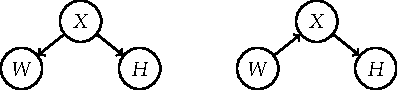
\includegraphics[width=0.7\textwidth,height=\textheight]{assets/causal-ex}
\caption{Causal diagrams for the heart disease examples.}
\end{figure}

The scenarios differ in the direction of the link between exercise and
weight gain.

Causal graphs are convenient when the exact assignments in a structural
causal models are of secondary importance, but what matters are the
paths present and absent in the graph. Graphs also let us import the
established language of graph theory to discuss causal notions. We can
say, for example, that an \emph{indirect cause}\index{cause!indirect} of
a node is any ancestor of the node in a given causal graph. In
particular, causal graphs allow us to distinguish cause and effect based
on whether a node is an ancestor or descendant of another node.

Let's take a first glimpse at a few important graph structures.

\hypertarget{forks}{%
\subsection{Forks}\label{forks}}

A \emph{fork} is a node~\(Z\) in a graph that has outgoing edges to two
other variables~\(X\) and~\(Y\). Put differently, the node~\(Z\) is a
common cause of~\(X\) and
\(Y\).\index{fork}\index{cause!common}\index{confounder}

\begin{figure}
\centering
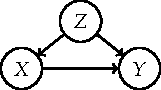
\includegraphics[width=0.3\textwidth,height=\textheight]{assets/causal-conf}
\caption{Example of a fork.}
\end{figure}

We already saw an example of a fork in our weight and exercise example:
\(W\leftarrow X \rightarrow H\). Here, exercise~\(X\) influences both
weight and heart disease. We also learned from the example that~\(Z\)
has a \emph{confounding}\index{confounding} effect: Ignoring
exercise~\(X\), we saw that~\(W\) and~\(H\) appear to be positively
correlated. However, the correlation is a mere result of confounding.
Once we hold exercise levels constant (via the do-operation), weight has
no effect on heart disease in our example.

Confounding leads to a disagreement between the calculus of conditional
probabilities (observation) and do-interventions (actions).

Real-world examples of confounding are a common threat to the validity
of conclusions drawn from data. For example, in a well known medical
study a suspected beneficial effect of \emph{hormone replacement
therapy} in reducing cardiovascular disease disappeared after
identifying \emph{socioeconomic status} as a confounding
variable.\footnote{Humphrey, Chan, and Sox, {``{Postmenopausal Hormone
  Replacement Therapy and the Primary Prevention of Cardiovascular
  Disease},''} \emph{Annals of Internal Medicine} 137, no. 4 (August
  2002): 273--84.}

\hypertarget{mediators}{%
\subsection{Mediators}\label{mediators}}

The case of a fork is quite different from the situation where~\(Z\)
lies on a directed path from~\(X\) to~\(Y\):

\begin{figure}
\centering
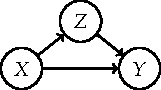
\includegraphics[width=0.3\textwidth,height=\textheight]{assets/causal-chain}
\caption{Example of a mediator.}
\end{figure}

In this case, the path~\(X\to Z\to Y\) contributes to the total effect
of \(X\) on~\(Y\). It's a causal path and thus one of the ways in
which~\(X\) causally influences~\(Y\). That's why~\(Z\) is not a
confounder. We call~\(Z\) a \emph{mediator} instead.\index{mediator}

We saw a plausible example of a mediator in our UC Berkeley admissions
example. In one plausible causal graph, department choice mediates the
influences of gender on the admissions decision.

\hypertarget{colliders}{%
\subsection{Colliders}\label{colliders}}

Finally, let's consider another common situation: the case of a
\emph{collider}.\index{collider}\index{explaining away}\index{Berkson's law}

\begin{figure}
\centering
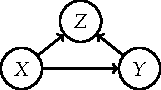
\includegraphics[width=0.3\textwidth,height=\textheight]{assets/causal-collider}
\caption{Example of a collider.}
\end{figure}

Colliders aren't confounders. In fact, in the above graph,~\(X\)
and~\(Y\) are unconfounded, meaning that we can replace do-statements by
conditional probabilities. However, something interesting happens when
we condition on a collider. The conditioning step can create correlation
between~\(X\) and~\(Y\), a phenomenon called \emph{explaining away}. A
good example of the explaining away effect, or \emph{collider bias}, is
due to Berkson. Two independent diseases can become negatively
correlated when analyzing hospitalized patients. The reason is that when
either disease (\(X\) or~\(Y\)) is sufficient for admission to the
hospital (indicated by variable~\(Z\)), observing that a patient has one
disease makes the other statistically less likely.\footnote{See the
  \href{https://en.wikipedia.org/wiki/Berkson\%27s_paradox}{Wikipedia
  article} and the reprint of Berkson's original article (Berkson,
  {``Limitations of the Application of Fourfold Table Analysis to
  Hospital Data,''} \emph{International Journal of Epidemiology} 43, no.
  2 (2014): 511--15).}

Berkson's law is a cautionary tale for statistical analysis when we're
studying a cohort that has been subjected to a selection rule. For
example, there's an ongoing debate about the effectiveness of GRE scores
in higher education. Recent studies\footnote{Moneta-Koehler, {``The
  Limitations of the GRE in Predicting Success in Biomedical Graduate
  School,''} \emph{PLOS ONE} 12, no. 1 (January 2017): 1--17; Hall,
  {``Predictors of Student Productivity in Biomedical Graduate School
  Applications,''} \emph{PLOS ONE} 12, no. 1 (January 2017): 1--14.}
argue that GRE scores are not predictive of various success outcomes in
a graduate student population. However, if such studies are restricted
to admitted students, this introduces the potential for collider bias.
The selection rule that introduces the potential for collider bias, and
care must be taken to tease out such effects.

\hypertarget{interventions-and-causal-effects}{%
\section{Interventions and causal
effects}\label{interventions-and-causal-effects}}

Structural causal models give us a way to formalize the effect of
hypothetical actions or interventions on the population within the
assumptions of our model. As we saw earlier all we needed was the
ability to do substitutions.\index{intervention}\index{causal!effect}

\hypertarget{substitutions-and-the-do-operator}{%
\subsection{Substitutions and the
do-operator}\label{substitutions-and-the-do-operator}}

Given a structural causal model~\(M\) we can take any assignment of the
form \[
X := f(P, U)
\] and replace it by another assignment. The most common substitution is
to assign~\(X\) a constant value~\(x\): \[
X := x
\] We will denote the resulting model by~\(M'=M[X:=x]\) to indicate the
surgery we performed on the original model~\(M\). Under this assignment
we hold~\(X\) constant by removing the influence of its parent nodes and
thereby any other variables in the model.

Graphically, the operation corresponds to eliminating all incoming edges
to the node~\(X\). The children of~\(X\) in the graph now receive a
fixed message~\(x\) from~\(X\) when they query the node's value.

\begin{figure}
\centering
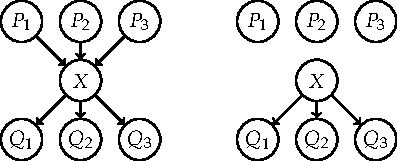
\includegraphics[width=0.6\textwidth,height=\textheight]{assets/causal-sub}
\caption{Graph before and after substitution.}
\end{figure}

The assignment operator is also called the
\emph{do-operator}\index{do-operator} to emphasize that it corresponds
to performing an action or intervention. We already have notation to
compute probabilities after applying the do-operator,
namely,~\(\mathbb{P}_{M[X:=x]}(E).\)

Another notation is popular and common: \[
\mathbb{P}\{E\mid \mathrm{do}(X:=x)\} = \mathbb{P}_{M[X:=x]}(E)
\]

This notation analogizes the do-operation with the usual notation for
conditional probabilities, and is often convenient when doing
calculations involving the do-operator. Keep in mind, however, that the
do-operator (action) is fundamentally different from the conditioning
operator (observation).

\hypertarget{causal-effects}{%
\subsection{Causal effects}\label{causal-effects}}

The \emph{causal effect} of an action~\(X:=x\) on a variable~\(Y\)
refers to the distribution of the variable~\(Y\) in the
model~\(M[X:=x].\) When we speak of the causal effect of a
variable~\(X\) on another variable~\(Y\) we refer to all the ways in
which setting~\(X\) to any possible value~\(x\) affects the distribution
of~\(Y\).\index{causal!effect}

Often we think of~\(X\) as a binary treatment variable and are
interested in a quantity such as \[
\mathbb{E}_{M[X:=1]}[Y] - \mathbb{E}_{M[X:=0]}[Y]\,.
\] This quantity is called the \emph{average treatment
effect}\index{treatment effect!average}. It tells us how much treatment
(action~\(X:=1\)) increases the expectation of~\(Y\) relative to no
treatment (action~\(X:=0\)).

Causal effects are population quantities. They refer to effects averaged
over the whole population. Often the effect of treatment varies greatly
from one individual or group of individuals to another. Such treatment
effects are called \emph{heterogeneous}.

\hypertarget{confounding}{%
\section{Confounding}\label{confounding}}

Important questions in causality relate to when we can rewrite a
do-operation in terms of conditional probabilities. When this is
possible, we can estimate the effect of the do-operation from
conventional conditional probabilities that we can estimate from data.

The simplest question of this kind asks when a causal effect
\(\mathbb{P}\{Y=y\mid \mathrm{do}(X:=x)\}\) coincides with the condition
probability~\(\mathbb{P}\{Y=y\mid X=x\}.\) In general, this is not true.
After all, the difference between observation (conditional probability)
and action (interventional calculus) is what motivated the development
of causality.

The disagreement between interventional statements and conditional
statements is so important that it has a well-known name:
\emph{confounding}\index{confounding}. We say that~\(X\) and~\(Y\) are
confounded when the causal effect of action~\(X:=x\) on~\(Y\) does not
coincide with the corresponding conditional probability.

When~\(X\) and~\(Y\) are confounded, we can ask if there is some
combination of conditional probability statements that give us the
desired effect of a do-intervention. This is generally possible given a
causal graph by conditioning on the parent nodes~\(\mathit{PA}\) of the
node~\(X\): \[
\mathbb{P}\{Y=y\mid \mathrm{do}(X:=x)\}
= \sum_z \mathbb{P}\{Y=y\mid X=x, \mathit{PA} = z\}
\mathbb{P}\{\mathit{PA} = z\}
\] This formula is called the \emph{adjustment
formula}\index{adjustment formula}. It gives us one way of estimating
the effect of a do-intervention in terms of conditional probabilities.

The adjustment formula is one example of what is often called
\emph{controlling for} a set of variables: We estimate the effect
of~\(X\) on \(Y\) separately in every slice of the population defined by
a condition \(Z=z\) for every possible value of~\(z\). We then average
these estimated sub-population effects weighted by the probability
of~\(Z=z\) in the population. To give an example, when we control for
age, we mean that we estimate an effect separately in each possible age
group and then average out the results so that each age group is
weighted by the fraction of the population that falls into the age
group.

Controlling for more variables in a study isn't always the right choice.
It depends on the graph structure. Let's consider what happens when we
control for the variable~\(Z\) in the three causal graphs we discussed
above.

\begin{itemize}
\tightlist
\item
  Controlling for a confounding variable \(Z\) in a fork
  \(X \leftarrow Z \rightarrow Y\) will deconfound the effect of \(X\)
  on \(Y\).
\item
  Controlling for a mediator \(Z\) will eliminate some of the causal
  influence of \(X\) on \(Y\).
\item
  Controlling for a collider will create correlation between \(X\) and
  \(Y\). That is the opposite of what controlling for \(Z\) accomplishes
  in the case of a fork. The same is true if we control for a descendant
  of a collider.
\end{itemize}

\hypertarget{the-backdoor-criterion}{%
\subsection{The backdoor criterion}\label{the-backdoor-criterion}}

At this point, we might worry that things get increasingly complicated.
As we introduce more nodes in our graph, we might fear a combinatorial
explosion of possible scenarios to discuss. Fortunately, there are
simple sufficient criteria for choosing a set of deconfounding variables
that is safe to control for.

A well known graph-theoretic notion is the
\emph{backdoor}\index{backdoor criterion} criterion.\footnote{Pearl,
  \emph{Causality}.} Two variables are confounded if there is a
so-called \emph{backdoor} path between them. A \emph{backdoor path}
from~\(X\) to \(Y\) is any path starting at~\(X\) with a backward edge
``\(\leftarrow\)'' into \(X\) such as:
\[ X \leftarrow A \rightarrow B \leftarrow C \rightarrow Y \]
Intuitively, backdoor paths allow information flow from~\(X\) to~\(Y\)
in a way that is not causal. To deconfound a pair of variables we need
to select a \emph{backdoor set} of variables that ``blocks'' all
backdoor paths between the two nodes. A backdoor path involving a chain
\(A\rightarrow B\rightarrow C\) can be blocked by controlling for~\(B\).
Information by default cannot flow through a collider
\(A\rightarrow B\leftarrow C\). So we only have to be careful not to
open information flow through a collider by conditioning on the
collider, or descendant of a collider.\footnote{For additional
  discussion of backdoor paths and confounding, see (Pearl).}

\hypertarget{unobserved-confounding}{%
\subsection{Unobserved confounding}\label{unobserved-confounding}}

The adjustment formula might suggest that we can always eliminate
confounding bias by conditioning on the parent nodes. However, this is
only true in the absence of \emph{unobserved
confounding}\index{confounding!unobserved}. In practice often there are
variables that are hard to measure, or were simply left unrecorded. We
can still include such unobserved nodes in a graph, typically denoting
their influence with dashed lines, instead of solid lines.

\begin{figure}
\centering
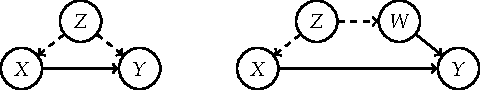
\includegraphics[width=0.75\textwidth,height=\textheight]{assets/causal-unob-conf}
\caption{Two cases of unobserved confounding.}
\end{figure}

The above figure shows two cases of unobserved confounding. In the first
example, the causal effect of~\(X\) on~\(Y\) is unidentifiable. In the
second case, we can block the confounding backdoor path
\(X\leftarrow Z\rightarrow W\rightarrow Y\) by controlling for~\(W\)
even though~\(Z\) is not observed. The backdoor criterion lets us work
around unobserved confounders in some cases where the adjustment formula
alone wouldn't suffice.

Unobserved confounding nonetheless remains a major obstacle in practice.
The issue is not just lack of measurement, but often lack of
anticipation or awareness of a confounding variable. We can try to
combat unobserved confounding by increasing the number of variables
under consideration. But as we introduce more variables into our study,
we also increase the burden of coming up with a valid causal model for
all variables under consideration. In practice, it is not uncommon to
control for as many variables as possible in a hope to disable
confounding bias. However, as we saw, controlling for mediators or
colliders can be harmful.

\hypertarget{randomization}{%
\subsection{Randomization}\label{randomization}}

The backdoor criterion gives a non-experimental way of eliminating
confounding bias given a causal model and a sufficient amount of
observational data from the joint distribution of the variables. An
alternative experimental method of eliminating confounding bias is the
well-known \emph{randomized controlled trial}.

In a \emph{randomized controlled
trial}\index{randomized controlled trial} a group of subjects is
randomly partitioned into a \emph{control group} and a \emph{treatment
group}. Participants do not know which group they were assigned to and
neither do the staff administering the trial. The control group receives
an actual treatment, such as a drug that is being tested for efficacy,
while the control group receives a placebo identical in appearance. An
outcome variable is measured for all
subjects.\index{control group}\index{treatment group}

The goal of a randomized controlled trial is to break natural
inclination. Rather than observing who chose to be treated on their own,
we assign treatment randomly. Thinking in terms of causal models, what
this means is that we eliminate all incoming edges into the treatment
variable. In particular, this closes all backdoor paths and hence avoids
confounding bias.

\hypertarget{counterfactuals}{%
\section{Counterfactuals}\label{counterfactuals}}

Fully specified structural causal models allow us to ask causal
questions that are more delicate than the mere effect of an action.
Specifically, we can ask \emph{counterfactual}\index{counterfactual}
questions such as: Would I have avoided the traffic jam had I taken a
different route this morning? Counterfactual questions are common. We
can answer them given a structural causal model. However, the procedure
for extracting the answer from the model looks a bit subtle at first. It
helps to start with a simple example.

\hypertarget{a-simple-counterfactual}{%
\subsection{A simple counterfactual}\label{a-simple-counterfactual}}

To understand counterfactuals, we first need to convince ourselves that
they aren't quite as straightforward as a single substitution in our
model.

Assume every morning we need to decide between two routes~\(X=0\) and
\(X=1\). On bad traffic days, indicated by~\(U=1\), both routes are bad.
On good days, indicated by~\(U=0\), the traffic on either route is good
unless there was an accident on the route.

Let's say that~\(U\sim B(1/2)\) follows the distribution of an unbiased
coin toss. Accidents occur independently on either route with
probability~\(1/2.\) So, choose two Bernoulli random variables
\(U_0, U_1\sim B(1/2)\) that tell us if there is an accident on
route~\(0\) and route~\(1\), respectively.

We reject all external route guidance and instead decide on which route
to take uniformly at random. That is,~\(X:=U_X\sim B(1/2)\) is also an
unbiased coin toss.

Introduce a variable~\(Y\in\{0,1\}\) that tells us whether the traffic
on the chosen route is good (\(Y=0\)) or bad (\(Y=1\)). Reflecting our
discussion above, we can express~\(Y\) as \[
Y := X\cdot \max\{U, U_1\} + (1-X)\max\{U, U_0\} \,.
\] In words, when~\(X=0\) the first term disappears and so traffic is
determined by the larger of the two values~\(U\) and~\(U_0\). Similarly,
when~\(X=1\) traffic is determined by the larger of~\(U\) and~\(U_1\).

\begin{figure}
\centering

\includegraphics[width=0.25\textwidth,height=\textheight]{assets/causal-counterf}
\caption{Causal diagram for our traffic scenario.}
\end{figure}

Now, suppose one morning we have~\(X=1\) and we observe bad
traffic~\(Y=1.\) Would we have been better off taking the alternative
route this morning?

A natural attempt to answer this question is to compute the likelihood
of~\(Y=0\) after the do-operation~\(X:=0\), that is,
\(\mathbb{P}_{M[X:=0]}(Y=0).\) A quick calculation reveals that this
probability is~\(\frac12 \cdot \frac12 = 1/4.\) Indeed, given the
substitution~\(X:=0\) in our model, for the traffic to be good we need
that~\(\max\{U, U_0\}=0.\) This can only happen when both~\(U=0\)
(probability~\(1/2\)) and~\(U_0=0\) (probability~\(1/2\)).

But this isn't the correct answer to our question. The reason is that we
took route~\(X=1\) and observed that~\(Y=1.\) From this observation, we
can deduce that certain background conditions did not manifest for they
are inconsistent with the observed outcome. Formally, this means that
certain settings of the noise variables~\((U, U_0, U_1)\) are no longer
feasible given the observed event~\(\{Y=1, X=1\}\). Specifically,
if~\(U\) and~\(U_1\) had both been zero, we would have seen no bad
traffic on route \(X=1\), but this is contrary to our observation. In
fact, the available evidence~\(\{Y=1, X=1\}\) leaves only the following
settings for~\(U\) and \(U_1\):\footnote{We leave out~\(U_0\) from the
  table, since its distribution is unaffected by our observation.}

\begin{longtable}[]{@{}cc@{}}
\caption{Possible noise settings after observing
evidence}\tabularnewline
\toprule
\(U\) & \(U_1\) \\
\midrule
\endfirsthead
\toprule
\(U\) & \(U_1\) \\
\midrule
\endhead
0 & 1 \\
1 & 1 \\
1 & 0 \\
\bottomrule
\end{longtable}

Each of these three cases is equally likely, which in particular means
that the event~\(U=1\) now has probability~\(2/3.\) In the absence of
any additional evidence, recall,~\(U=1\) had probability~\(1/2.\) What
this means is that the observed evidence~\(\{Y=1, X=1\}\) has biased the
distribution of the noise variable~\(U\) toward~\(1\). Let's use the
letter \(U'\) to refer to this biased version of~\(U\).\footnote{Formally,~\(U'\)
  is distributed according to the distribution of~\(U\) conditional on
  the event~\(\{Y=1, X=1\}.\)}

Working with this biased noise variable, we can again entertain the
effect of the action~\(X:=0\) on the outcome~\(Y\). For~\(Y=0\) we need
that \(\max\{U', U_0\}=0.\) This means that~\(U'=0\), an event that now
has probability~\(1/3\), and~\(U_0=0\) (probability~\(1/2\) as before).
Hence, we get the probability~\(1/6=1/2\cdot 1/3\) for the event
that~\(Y=0\) under our do-operation~\(X:=0\), and after updating the
noise variables to account for the observation~\(\{Y=1, X=1\}\).

To summarize, incorporating available evidence into our calculation
decreased the probability of no traffic (\(Y=0\)) when choosing
route~\(0\) from~\(1/4\) to~\(1/6\). The intuitive reason is that the
evidence made it more likely that it was generally a bad traffic day,
and even the alternative route would've been clogged. More formally, the
event that we observed biases the distribution of exogenous noise
variables.

We think of the result we just calculated as the \emph{counterfactual}
of choosing the alternative route given the route we chose had bad
traffic.

\hypertarget{the-general-recipe}{%
\subsection{The general recipe}\label{the-general-recipe}}

We can generalize our discussion of computing counterfactuals from the
previous example to a general procedure. There were three essential
steps. First, we incorporated available observational evidence by
biasing the exogenous noise variables through a conditioning operation.
Second, we performed a do-operation in the structural causal model after
we substituted the biased noise variables. Third, we computed the
distribution of a target variable.

These three steps are typically called \emph{abduction}, \emph{action},
and \emph{prediction}, as can be described as follows.

\begin{Definition}

Given a structural causal model~\(M\), an observed event~\(E\), an
action \(X:= x\) and target variable~\(Y,\) we define the
\emph{counterfactual} \(Y_{X:=x}(E)\) by the following three step
procedure:

\begin{enumerate}
\def\labelenumi{\arabic{enumi}.}
\tightlist
\item
  \textbf{Abduction:} Adjust noise variables to be consistent with the
  observed event. Formally, condition the joint distribution of
  \(U=(U_1,...,U_d)\) on the event \(E\). This results in a biased
  distribution \(U'\).
\item
  \textbf{Action:} Perform do-intervention \(X:=x\) in the structural
  causal model \(M\) resulting in the model \(M'=M[X:=x].\)
\item
  \textbf{Prediction:} Compute target counterfactual \(Y_{X:=x}(E)\) by
  using \(U'\) as the random seed in \(M'.\)
\end{enumerate}

\end{Definition}

It's important to realize that this procedure \emph{defines} what a
counterfactual is in a structural causal model. The notation
\(Y_{X:=x}(E)\) denotes the outcome of the procedure and is part of the
definition. We haven't encountered this notation before.

Put in words, we interpret the formal counterfactual~\(Y_{X:=x}(E)\) as
the value~\(Y\) would've taken had the variable~\(X\) been set to
value~\(x\) in the circumstances described by the event~\(E\).

In general, the counterfactual~\(Y_{X:=x}(E)\) is a random variable that
varies with~\(U'\). But counterfactuals can also be deterministic. When
the event~\(E\) narrows down the distribution of~\(U\) to a single point
mass, called \emph{unit}, the variable~\(U'\) is constant and hence the
counterfactual~\(Y_{X:=x}(E)\) reduces to a single number. In this case,
it's common to use the shorthand
notation~\(Y_{x}(u)=Y_{X:=x}(\{U=u\}),\) where we make the
variable~\(X\) implicit, and let~\(u\) refer to a single unit.

The motivation for the name \emph{unit} derives from the common
situation where the structural causal model describes a population of
entities that form the atomic units of our study. It's common for a unit
to be an individual (or the description of a single individual).
However, depending on application, the choice of units can vary. In our
traffic example, the noise variables dictate which route we take and
what the road conditions are.

Answers to counterfactual questions strongly depend on the specifics of
the structural causal model, including the precise model of how the
exogenous noise variables come into play. It's possible to construct two
models that have identical graph structures, and behave identically
under interventions, yet give different answers to counterfactual
queries.\footnote{Peters, Janzing, and Schölkopf, \emph{Elements of
  Causal Inference} (MIT Press, 2017).}

\hypertarget{potential-outcomes}{%
\subsection{Potential outcomes}\label{potential-outcomes}}

The \emph{potential outcomes}\index{potential outcomes} framework is a
popular formal basis for causal inference, which goes about
counterfactuals differently. Rather than deriving them from a structural
causal model, we assume their existence as ordinary random variables,
albeit some unobserved.

Specifically, we assume that for every unit~\(u\) there exist random
variables~\(Y_x(u)\) for every possible value of the assignment~\(x\).
In the potential outcomes model, it's customary to think of a binary
\emph{treatment variable} \(X\) so that~\(x\) assumes only two
values,~\(0\) for \emph{untreated}, and~\(1\) for \emph{treated}. This
gives us two potential outcome variables~\(Y_0(u)\) and~\(Y_1(u)\) for
each unit~\(u\).\footnote{There is some potential for notational
  confusion here. Readers familiar with the potential outcomes model may
  be used to the notation ``\(Y_i(0), Y_i(1)\)'' for the two potential
  outcomes corresponding to unit~\(i\). In our notation the unit (or,
  more generally, set of units) appears in the parentheses and the
  subscript denotes the substituted value for the variable we intervene
  on.}

The key point about the potential outcomes model is that we only observe
the potential outcome~\(Y_1(u)\) for units that were treated. For
untreated units we observe~\(Y_0(u)\). In other words, we can never
simultaneously observe both, although they're both assumed to exist in a
formal sense. Formally, the outcome~\(Y(u)\) for unit~\(u\) that we
observe depends on the binary treatment~\(T(u)\) and is given by the
expression: \[Y(u)=Y_0(u)\cdot(1-T(u))+Y_1(u) \cdot T(u)\] It's often
convenient to omit the parentheses from our notation for counterfactuals
so that this expression would read~\(Y=Y_0\cdot(1-T)+Y_1\cdot T\).

We can revisit our traffic example in this framework. The next table
summarizes what information is observable in the potential outcomes
model. We think of the route we choose as the treatment variable, and
the observed traffic as reflecting one of the two potential outcomes.

\begin{longtable}[]{@{}cccr@{}}
\caption{Traffic example in the potential outcomes model}\tabularnewline
\toprule
Route \(X\) & Outcome \(Y_0\) & Outcome \(Y_1\) & Probability \\
\midrule
\endfirsthead
\toprule
Route \(X\) & Outcome \(Y_0\) & Outcome \(Y_1\) & Probability \\
\midrule
\endhead
0 & 0 & ? & 1/8 \\
0 & 1 & ? & 3/8 \\
1 & ? & 0 & 1/8 \\
1 & ? & 1 & 3/8 \\
\bottomrule
\end{longtable}

Often this information comes in the form of samples. For example, we
might observe the traffic on different days. With sufficiently many
samples, we can estimate the above frequencies with arbitrary accuracy.

\begin{longtable}[]{@{}cccc@{}}
\caption{Traffic data in the potential outcomes model}\tabularnewline
\toprule
Day & Route \(X\) & Outcome \(Y_0\) & Outcome \(Y_1\) \\
\midrule
\endfirsthead
\toprule
Day & Route \(X\) & Outcome \(Y_0\) & Outcome \(Y_1\) \\
\midrule
\endhead
1 & 0 & 1 & ? \\
2 & 0 & 0 & ? \\
3 & 1 & ? & 1 \\
4 & 0 & 1 & ? \\
5 & 1 & ? & 0 \\
\ldots{} & \ldots{} & \ldots{} & \ldots{} \\
\bottomrule
\end{longtable}

A typical query in the potential outcomes model is the \emph{average
treatment effect} \(\mathbb{E}[Y_1 - Y_0].\) Here the expectation is
taken over the properly weighted units in our study. If units correspond
to equally weighted individuals, the expectation is an average over
these individuals.

In our original traffic example, there were~\(16\) units corresponding
to the background conditions given by the four binary variables
\(U, U_0, U_1, U_X\). When the units in the potential outcome model
agree with those of a structural causal model, then causal effects
computed in the potential outcomes model agree with those computed in
the structural equation model. The two formal frameworks are perfectly
consistent with each other.

As is intuitive from the table above, causal inference in the potential
outcomes framework can be thought of as filling in the missing entries
(``?'') in the table above. This is sometimes called \emph{missing data
imputation} and there are numerous statistical methods for this task. If
we could \emph{reveal} what's behind the question marks, estimating the
average treatment effect would be as easy as counting rows.

There is a set of established conditions under which causal inference
becomes possible:

\begin{enumerate}
\def\labelenumi{\arabic{enumi}.}
\tightlist
\item
  \textbf{Stable Unit Treatment Value Assumption} (SUTVA): The treatment
  that one unit receives does not change the effect of treatment for any
  other unit.\index{SUTVA}
\item
  \textbf{Consistency}: Formally, \(Y=Y_0(1-T)+Y_1T.\) That is,
  \(Y=Y_0\) if \(T=0\) and \(Y=Y_1\) if \(T=1\). In words, the outcome
  \(Y\) agrees with the potential outcome corresponding to the treatment
  indicator.
\item
  \textbf{Ignorability}: The potential outcomes are independent of
  treatment given some deconfounding variables \(Z\), i.e.,
  \(T\bot (Y_0, Y_1)\mid Z\). In words, the potential outcomes are
  conditionally independent of treatment given some set of deconfounding
  variables.\index{ignorability}
\end{enumerate}

The first two assumptions automatically hold for counterfactual
variables derived from structural causal models according to the
procedure described above. This assumes that the units in the potential
outcomes framework correspond to the atomic values of the background
variables in the structural causal model.

The third assumption is a major one. It's easiest to think of it as
aiming to formalize the guarantees of a perfectly executed randomized
controlled trial. The assumption on its own cannot be verified or
falsified, since we never have access to samples with both potential
outcomes manifested. However, we can verify if the assumption is
consistent with a given structural causal model by checking if the set
\(Z\) blocks all backdoor paths from treatment~\(T\) to outcome~\(Y\).

There's no tension between structural causal models and potential
outcomes and there's no harm in having familiarity with both. It
nonetheless makes sense to say a few words about the differences of the
two approaches.

We can derive potential outcomes from a structural causal model as we
did above, but we cannot derive a structural causal model from potential
outcomes alone. A structural causal model in general encodes more
assumptions about the relationships of the variables. This has several
consequences. On the one hand, a structural causal model gives us a
broader set of formal concepts (causal graphs, mediating paths,
counterfactuals for every variable, and so on). On the other hand,
coming up with a plausibly valid structural causal model is often a
daunting task that might require knowledge that is simply not available.
We will dive deeper into questions of validity below. Difficulty to come
up with a plausible causal model often exposes unsettled substantive
questions that require resolution first.

The potential outcomes model, in contrast, is generally easier to apply.
There's a broad set of statistical estimators of causal effects that can
be readily applied to observational data. But the ease of application
can also lead to abuse. The assumptions underpinning the validity of
such estimators are experimentally unverifiable. Frivolous application
of causal effect estimators in situations where crucial assumptions do
not hold can lead to false results, and consequently to ineffective or
harmful interventions.

\hypertarget{chapter-notes-8}{%
\section{Chapter notes}\label{chapter-notes-8}}

This chapter overlaps significantly with the chapter on causality in the
textbook on fairness and machine learning by Barocas, Hardt, and
Narayanan,\footnote{Barocas, Hardt, and Narayanan, \emph{Fairness and
  Machine Learning}.} which contains additional discussion of
discrimination and fairness analysis.

There are several excellent introductory textbooks on the topic of
causality. For an introduction to causality with an emphasis on causal
graphs and structural equation models turn to Pearl's primer,\footnote{Pearl,
  Glymour, and Jewell, \emph{Causal Inference in Statistics: A Primer}
  (Wiley, 2016).} or the more comprehensive textbook.\footnote{Pearl,
  \emph{Causality}.} Our exposition of Simpson's paradox and the UC
Berkeley data was influenced by Pearl's discussion, updated for a new
popular audience book.\footnote{Pearl and Mackenzie, \emph{The Book of
  Why}.} The technically-minded reader will enjoy complementing Pearl's
book with the recent open access text by Peters, Janzing, and
Schölkopf\footnote{Peters, Janzing, and Schölkopf, \emph{Elements of
  Causal Inference}.} that is
\href{https://mitpress.mit.edu/books/elements-causal-inference}{available
online}. The text emphasizes two variable causal models and applications
to machine learning. See Spirtes, Glymour and Scheines\footnote{Spirtes
  et al., \emph{Causation, Prediction, and Search} (MIT press, 2000).}
for a general introduction based on causal graphs with an emphasis on
\emph{graph discovery}, i.e., inferring causal graphs from observational
data. Morgan and Winship\footnote{Morgan and Winship,
  \emph{Counterfactuals and Causal Inference} (Cambridge University
  Press, 2014).} focus on applications in the social sciences. Imbens
and Rubin\footnote{Imbens and Rubin, \emph{Causal Inference for
  Statistics, Social, and Biomedical Sciences} (Cambridge University
  Press, 2015).} give a comprehensive introduction to the technical
repertoire of causal inference in the potential outcomes model. Angrist
and Pischke\footnote{Angrist and Pischke, \emph{Mostly Harmless
  Econometrics: An Empiricist's Companion} (Princeton university press,
  2008).} focus on causal inference and potential outcomes in
econometrics. Hernán and Robins\footnote{Hernán and Robins, \emph{Causal
  Inference} (Boca Raton: Chapman \& Hall/CRC, forthcoming, 2019).} give
another detailed introduction to causal inference, also
\href{https://www.hsph.harvard.edu/miguel-hernan/causal-inference-book/}{available
online}, that draws on the authors' experience in epidemiology.

\chapter{Causal inference in practice}

The previous chapter introduced the conceptual foundations of causality,
but there's a lot more to learn about how these concepts play out in
practice. In fact, there's a flourishing practice of causal inference in
numerous scientific disciplines. Increasingly, ideas from machine
learning show up in the design of causal estimators. Conversely, ideas
from causal inference can help machine learning practitioners run better
experiments.

In this chapter we focus on estimating the average treatment effect,
often abbreviated as ATE, of a binary treatment~\(T\) on an outcome
variable~\(Y\): \[
\mathop\mathbb{E}[Y \mid \mathrm{do}(T:=1) ] - \mathop\mathbb{E}[Y \mid \mathrm{do}(T:=0)]\,.
\] Causal effects are population quantities that involve two
hypothetical actions, one holding the treatment variable constant at the
treatment value~\(1\), the other holding the treatment constant at its
baseline value~\(0\).

The central question in causal inference is how we can estimate causal
quantities, such as the average treatment effect, from data.

Confounding between the outcome and treatment variable is the main
impediment to causal inference from observational data. Recall that
random variables~\(Y\) and~\(T\) are confounded, if the conditional
probability distribution of~\(Y\) given~\(T\) does not equal its
interventional counterpart: \[
\mathop\mathbb{P}\{Y=y\mid \mathrm{do}(T:=t)\}
\ne
\mathop\mathbb{P}\{Y=y\mid T=t\}
\] If these expressions were equal, we could estimate the average
treatment effect in a straightforward way by estimating the difference
\(\mathop\mathbb{E}[Y\mid T=1]-\mathop\mathbb{E}[Y\mid T=0]\) from
samples. Confounding makes the estimation of treatment effects more
challenging, and sometimes impossible. Note that the main challenge here
is to arrive at an expression for the desired causal effect that is free
of any causal constructs, such as the do-operator. Once we have a plain
probability expression at hand, tools from statistics allow us to relate
the population quantity with a finite sample estimate.

\hypertarget{design-and-inference}{%
\section{Design and inference}\label{design-and-inference}}

There are two important components to causal inference, one is
\emph{design}, the other is \emph{inference}.

In short, design is about sorting out various substantive questions
about the data generating process. Inference is about the statistical
apparatus that we unleash on the data in order to estimate a desired
causal effect.

Design requires us to decide on a population, a set of variables to
include, and a precise question to ask. In this process we need to
engage substantively with relevant scientific domain knowledge in order
to understand what assumptions we can make about the data.

Design can only be successful if the assumptions we are able to make
permit the estimation of the causal effect we're interested in. In
particular, this is where we need to think carefully about potential
sources of confounding and how to cope with them.

There is no way statistical estimators can recover from poor design. If
the design does not permit causal inference, there is simply no way that
a clever statistical trick could remedy the shortcoming. It's therefore
apt to think of causal insights as consequences of the substantive
assumptions that we can make about the data, rather than as products of
sophisticated statistical ideas.

Hence, we emphasize design issues throughout this chapter and
intentionally do not dwell on technical statements about rates of
estimation. Such mathematical statements can be valuable, but design
must take precedence.

\hypertarget{experimental-and-observational-designs}{%
\subsection{Experimental and observational
designs}\label{experimental-and-observational-designs}}

Causal inference distinguishes between \emph{experimental} and
\emph{observational} designs. Experimental designs generally are active
in the sense of administering some treatment to some set of experimental
units. Observational designs do not actively assign treatment, but
rather aim to make it possible to identify causal effects from collected
data without implementing any interventions.

The most common and well-established experimental design is a randomized
controlled trial (RCT). The main idea is to assign treatment randomly. A
randomly assigned treatment, by definition, is not influenced by any
other variable. Hence, randomization eliminates any confounding bias
between treatment and outcome.

In a typical implementation of a randomized controlled trial, subjects
are randomly partitioned into a \emph{treatment group} and a
\emph{control group}. The treatment group receives the treatment, the
control group receives no treatment. It is important that subjects do
not know which group they were assigned to. Otherwise knowledge of their
assignment may influence the outcome. To ensure this, subjects in the
control group receive what is called a \emph{placebo}, a device or
procedure that looks indistinguishable from treatment to the study
subject, but lacks the treatment ingredient whose causal powers are in
question. Adequate placebos may not exist depending on what the
treatment is, for example, in the case of a surgery.

Randomized controlled trials have a long history with many success
stories. They've become an important source of scientific knowledge.

Sometimes randomized controlled trials are difficult, expensive, or
impossible to administer. Treatment might be physically or legally
impossible, too costly, or too dangerous. Nor are they free of issues
and pitfalls.\footnote{Deaton and Cartwright, {``Understanding and
  Misunderstanding Randomized Controlled Trials,''} \emph{Social Science
  \& Medicine} 210 (2018): 2--21.} In this chapter, we will see
observational alternatives to randomized controlled trials. However,
these are certainly not without their own set of difficulties and
shortcomings.

The machine learning practitioner is likely to encounter randomization
in the form of so-called \emph{A/B tests}. In an A/B test we randomly
assign one of two treatments to a set of individuals. Such experiments
are common in the tech industry to find out which of two changes to a
product leads to a better outcome.

\index{A/B test}

\hypertarget{the-observational-basics-adjustment-and-controls}{%
\section{The observational basics: adjustment and
controls}\label{the-observational-basics-adjustment-and-controls}}

For the remainder of the chapter we focus on observational causal
inference methods. In the previous chapter we saw that there are
multiple ways to cope with confounding between treatment and outcome.
One of them is to adjust (or control) for the parents (i.e., direct
causes) of~\(T\) via the adjustment formula.\index{adjustment formula}

The extra variables that we adjust for are also called \emph{controls},
and we take the phrase \emph{controlling for} to mean the same thing as
\emph{adjusting for}.

We then saw that we could use any set of random variables satisfying the
graphical backdoor criterion. This is helpful in cases where some direct
causes are unobserved so that we cannot use them in the adjustment
formula.

Let's generalize this idea even further and call a set of variables
\emph{admissible} if it satisfies the adjustment
formula.\index{admissible}

\begin{Definition}

We say that a discrete random variable~\(X\) is \emph{admissible} if it
satisfies the adjustment formula: \[
\mathop\mathbb{P}[Y=y\mid \mathrm{do}(T:=t)] = \sum_x \mathop\mathbb{P}[Y=y\mid T=t, X=x] \mathop\mathbb{P}[X=x]
\] Here we sum over all values~\(x\) in the support of~\(X\).

\end{Definition}

The definition directly suggests a basic estimator for the
do-intervention:

\begin{enumerate}
\def\labelenumi{\arabic{enumi}.}
\tightlist
\item
  Collect samples \(n\) samples \((t_i, y_i, x_i)_{i=1}^n.\)
\item
  Estimate each of the conditional probabilities
  \(\mathop\mathbb{P}[Y=y\mid T=t,X=x]\) from the collected samples.
\item
  Compute the weighted sum.
\end{enumerate}

This estimator can only work if all slices~\(\{T=t,X=x\}\) have nonzero
probability, an assumption often called \emph{overlap} or
\emph{positivity} in causal inference.\index{overlap}

But the basic estimator also fails when the adjustment variable~\(X\)
can take on too many possible values. In general, the variable~\(X\)
could correspond to a tuple of features, such as, age, height, weight,
etc. The support of~\(X\) grows exponentially with the number of
features. This poses an obvious computational problem, but more
importantly a statistical problem as well. By a counting argument some
of the events \(\{T=t,X=x\}\) must have probability as small as the
inverse of size of the support~\(X\). To estimate a probability~\(p>0\)
from samples to within small relative error, we need about~\(O(1/p^2)\)
samples.

Much work in causal inference deals with overcoming the statistical
inefficiency of the basic estimator. Conceptually, however, most
sophisticated estimators work from the same principle. We need to assume
that we have an admissible variable~\(X\) and that positivity holds.
Different estimators then use this assumption in different ways.

\hypertarget{potential-outcomes-and-ignorability}{%
\subsection{Potential outcomes and
ignorability}\label{potential-outcomes-and-ignorability}}

The average treatment effect often appears in the causal inference
literature equivalently in its potential outcome notation
\(\mathop\mathbb{E}[Y_1 - Y_0]\). This way of going about it is
mathematically equivalent and either way works for us.

When talking about potential outcomes, it's customary to replace the
assumption that~\(X\) is admissible with another essentially equivalent
assumption called \emph{ignorability} or \emph{unconfoundedness}. To
recall from the previous chapter, this assumption requires that the
potential outcomes variables are conditionally independent of treatment
given~\(X\). Formally,~\(T\bot (Y_0, Y_1)\mid X\). It's not hard to show
that ignorability implies that~\(X\) is
admissible.\index{unconfoundedness}\index{ignorability}

\hypertarget{reductions-to-model-fitting}{%
\section{Reductions to model
fitting}\label{reductions-to-model-fitting}}

Adjustment gives a simple and general way to estimate causal effects
given an admissible set of variables. The primary shortcoming that we
discussed is the sample inefficiency of the formula in high-dimensional
settings.

There's a vast literature of causal estimators that aim to address this
central shortcoming in a range of different settings. While the
landscape of causal estimators might seem daunting to newcomers, almost
all causal inference methods share a fundamental idea. This idea is
reduce causal inference to standard supervised machine learning tasks.

Let's see how this central idea plays out in a few important cases.

\hypertarget{propensity-scores}{%
\subsection{Propensity scores}\label{propensity-scores}}

Propensity scores are one popular way to cope with adjustment variables
that have large support.

Let~\(T \in \{ 0, 1 \}\) be a binary treatment variable. The quantity \[
e(x) = \mathop\mathbb{E}[T \mid X=x]
\] is known as the \emph{propensity score} and gives the likelihood of
treatment given in the subpopulation defined by the condition
\(X=x\).\index{propensity score}

\begin{Theorem}

Suppose that~\(X\) is admissible, and the propensity scores are positive
\(e(x) \neq 0\) for all~\(X\). Then, \[
\begin{aligned}
\mathop\mathbb{E}[ Y \mid \mathrm{do}(T := 1) ] = \mathop\mathbb{E} \left[ \frac{YT}{e(X)} \right]
\end{aligned}
\]

\end{Theorem}

\begin{Proof}

Applying the adjustment formula, we have \[
\begin{aligned}
\mathop\mathbb{E}[ Y \mid \mathrm{do}(T := 1)]
&= \sum_y y \mathop\mathbb{P}[Y = y \mid \mathrm{do}(T := 1)] \\
&= \sum_y y \left( \sum_x \mathop\mathbb{P}[ Y = y \mid T = 1, X=x] \mathop\mathbb{P}[X=x] \right)\\
&= \sum_y y \left( \sum_x \frac{\mathop\mathbb{P}[ Y = y \mid T= 1, X=x] \mathop\mathbb{P}[X=x] \mathop\mathbb{P}[T = 1 \mid X=x]}{\mathop\mathbb{P}[T = 1 \mid X=x]} \right)\\
&= \sum_y y \left( \sum_x \frac{\mathop\mathbb{P}[Y = y, T = 1, X=x]}{\mathop\mathbb{P}[T = 1 \mid X=x]} \right)\\
&= \sum_y y \left( \sum_{x, t\in\{0, 1\}} \frac{t \mathop\mathbb{P}[Y = y,T = t,X=x] }{\mathop\mathbb{P}[T = 1 \mid X=x]} \right)\\
&= \sum_{y, x, t\in\{0, 1\}}   \frac{y t \mathop\mathbb{P}[ Y = y, T = t,  X=x ]}{\mathop\mathbb{P}[T = 1 \mid X=x]} \\
&= \mathop\mathbb{E} \left[ \frac{YT}{e(X)} \right]
\end{aligned}
\] Here, we used the adjustment formula in the second line, then
multiplied and divided
by~\(e(x) = \mathop\mathbb{P}[T = 1 \mid X=x] \neq 0\) to obtain the
third line.

\end{Proof}

The same theorem also shows that \[
\mathop\mathbb{E}[Y \mid \mathrm{do}(T := 0) ] = \mathop\mathbb{E} \left[ \frac{Y(1 - T)}{1 - e(X)} \right]
\] and thus the average treatment effect of~\(X\) on~\(Y\) is given by
\[
\mathop\mathbb{E}[ Y \mid \mathrm{do}(T := 1)]
- \mathop\mathbb{E}[Y \mid \mathrm{do}(T := 0)]
= \mathop\mathbb{E} \left[ Y\left(\frac{T}{e(X)}-\frac{1-T}{1-e(X)}\right) \right]\,.
\] This formula for the average treatment effect is called \emph{inverse
propensity score weighting}. Let's understand what it buys us compared
with the adjustment formula when working with a finite sample.

One way to approximate the expectation given the the theorem above is to
collect many samples from which we estimate the propensity
score~\(e(x)\) separately for each possible setting~\(X\). However, this
way of going about it runs into the very same issues as the basic
estimator. Practitioners therefore choose a different route.

In a first step, we fit a model~\(\hat e\) to the propensity scores
hoping that our model~\(\hat e\) approximates the propensity score
function~\(e\) uniformly well. We approach this step as we would any
other machine learning problem. We create a dataset of
observations~\((x_i, e_i)\) where \(e_i\) is an empirical estimate
of~\(e(x_i)\) that we compute from our sample. We then fit a model to
these data points using our favorite statistical technique, be it
logistic regression or something more sophisticated.

In a second step, we then use our model's estimated propensity scores in
our sample estimate instead of the true propensity scores: \[
\frac{1}{n} \sum_{i=1}^n \frac{t_i y_i}{\hat e (x_i)}.
\] The appeal of this idea is that we can use the entire repertoire of
model fitting to get a good function approximation of the propensity
scores. Depending on what the features are we could use logistic
regression, kernel methods, random forests, or even deep models.
Effectively we're reducing the problem of causal inference to that of
model fitting, which we know how to do.

\hypertarget{double-machine-learning}{%
\subsection{Double machine learning}\label{double-machine-learning}}

Our previous reduction to model fitting has a notable shortcoming. The
propensity score estimate~\(\hat e(x_i)\) appears in the denominator of
our estimator. This has two consequences. First, unbiased estimates of
propensity scores do not imply an unbiased estimate of the causal
effect. Second, when propensity scores are small and samples aren't too
plentiful, this can lead to substantial variance.

There's a popular way to cope, called \emph{double machine learning},
that works in a partially linear structural causal
model:\marginnote{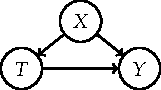
\includegraphics[width=0.3\textwidth,height=\textheight]{assets/causal-conf-TXY}}\index{double machine learning}
\[
\begin{aligned}
Y &= \tau T + g(X) + U \\
T &= f(X) + V
\end{aligned}
\] In this model, the variable~\(X\) is an observed confounder between
treatment and outcome. We allow the functions~\(g\) and~\(f\) to be
arbitrary, but note that~\(g\) only depends on~\(X\) but not on~\(T\) as
it could in general. The random variables~\(U, V\) are independent
exogenous noise variables with mean~\(0\). In this model, the effect of
treatment on the outcome is linear and the coefficient~\(\tau\) is the
desired average treatment effect.

The trick behind double machine learning is to
subtract~\(\mathop\mathbb{E}[Y\mid X]\) from each side of the first
equation and to use the fact that
\(\mathop\mathbb{E}[Y\mid X]=\tau\mathop\mathbb{E}[T\mid X] + g(X)\). We
therefore get the equation \[
Y-\mathop\mathbb{E}[Y\mid X] = \tau (T-\mathop\mathbb{E}[T\mid X]) + U\,.
\] Denoting~\(\tilde Y = Y-\mathop\mathbb{E}[Y\mid X]\)
and~\(\tilde T=T-\mathop\mathbb{E}[T\mid X]\) we can see that the causal
effect~\(\tau\) is the solution to the regression
problem~\(\tilde Y = \tau \tilde T+U\).

The idea now is to solve \emph{two} regression problems to find good
function approximations of the conditional
expectations~\(\mathop\mathbb{E}[Y\mid X]\) and
\(\mathop\mathbb{E}[T\mid X]\), respectively. We can do this using data
drawn from the joint distribution of~\((X, T, Y)\) by solving two
subsequent model fitting problems, hence the name double machine
learning.

Suppose then that we find two function approximations
\(q(X, Y) \approx \mathop\mathbb{E}[Y\mid X]\)
and~\(r(X, T)\approx\mathop\mathbb{E}[T\mid X]\). We can define the
random variables~\(\hat Y = Y - q(X, Y)\) and \(\hat T = T - r(X, T)\).
The final step is to solve the regression
problem~\(\hat Y = \hat\tau\hat T + U\) for the parameter~\(\hat\tau\).

Compared with inverse propensity score weighting, we can see that finite
sample errors in estimating the conditional expectations have a more
benign effect on the causal effect estimate~\(\hat\tau\). In particular,
unbiased estimates of the conditional expectations lead to an unbiased
estimate of the causal effect.

\hypertarget{heterogeneous-treatment-effects}{%
\subsection{Heterogeneous treatment
effects}\label{heterogeneous-treatment-effects}}

In many applications, treatment effects can vary by subpopulation. In
such cases we may be interested in the \emph{conditional average
treatment effect} (CATE) in the subpopulation defined by
\(X=x\):\index{treatment effect!conditional average}\index{treatment effect!heterogeneous}
\[
\tau(x)=\mathop\mathbb{E}[Y \mid \mathrm{do}(T:=1), X=x ] - \mathop\mathbb{E}[Y \mid \mathrm{do}(T:=0), X=x]\,.
\] We're in luck, because the same proof we saw earlier shows that we
can estimate these so-called heterogeneous treatment effects with the
propensity score formula: \[
\tau(x) = \mathop\mathbb{E}\left[Y\left(\frac{T}{e(X)}-\frac{1-T}{1-e(X)}\right)\mid X=x\right]
\]

We can also extend double machine learning easily to the heterogeneous
case by replacing the coefficient~\(\tau\) in the first structural
equation with a function~\(\tau(X)\) that depends on~\(X\). The argument
remains the same except that in the end we need to solve the problem
\(\hat Y = \hat\tau(X) \hat T + Y\), which amounts to optimizing over a
function~\(\hat\tau\) in some model family rather than a constant
\(\hat\tau\).

Both inverse propensity score weighting and the double machine learning
can, in principle, estimate heterogeneous treatment effects. These
aren't the only reductions to model fitting, however. Another popular
method, called \emph{causal forests}, constructs decision trees whose
leaves correspond covariate settings that deconfound treatment and
outcome.\footnote{Wager and Athey, {``Estimation and Inference of
  Heterogeneous Treatment Effects Using Random Forests,''} \emph{Journal
  of the American Statistical Association} 113, no. 523 (2018):
  1228--42.}\index{causal!forest}

\hypertarget{quasi-experiments}{%
\section{Quasi-experiments}\label{quasi-experiments}}

The idea behind quasi-experimental designs is that sometimes processes
in nature or society are structured in a way that enables causal
inference. The three most widely used quasi-experimental designs are
\emph{regression discontinuities}, \emph{instrumental variables}, and
\emph{differences in differences}. We will review the first two briefly
to see where machine learning comes
in.\index{regression discontinuity}\index{instrumental variables}\index{differences in differences}\index{quasi-experiments}

\hypertarget{regression-discontinuity}{%
\subsection{Regression discontinuity}\label{regression-discontinuity}}

Many consequential interventions in society trigger when a certain score
\(R\) exceeds a threshold value~\(t\). The idea behind a regression
discontinuity design is that units that fall just below the threshold
are indistinguishable from units just above threshold. In other words,
whether or not a unit is just above or just below the threshold is a
matter of pure chance. We can then hope to identify a causal effect of
an intervention by comparing units just below and just above the
threshold.

\begin{figure}
\centering
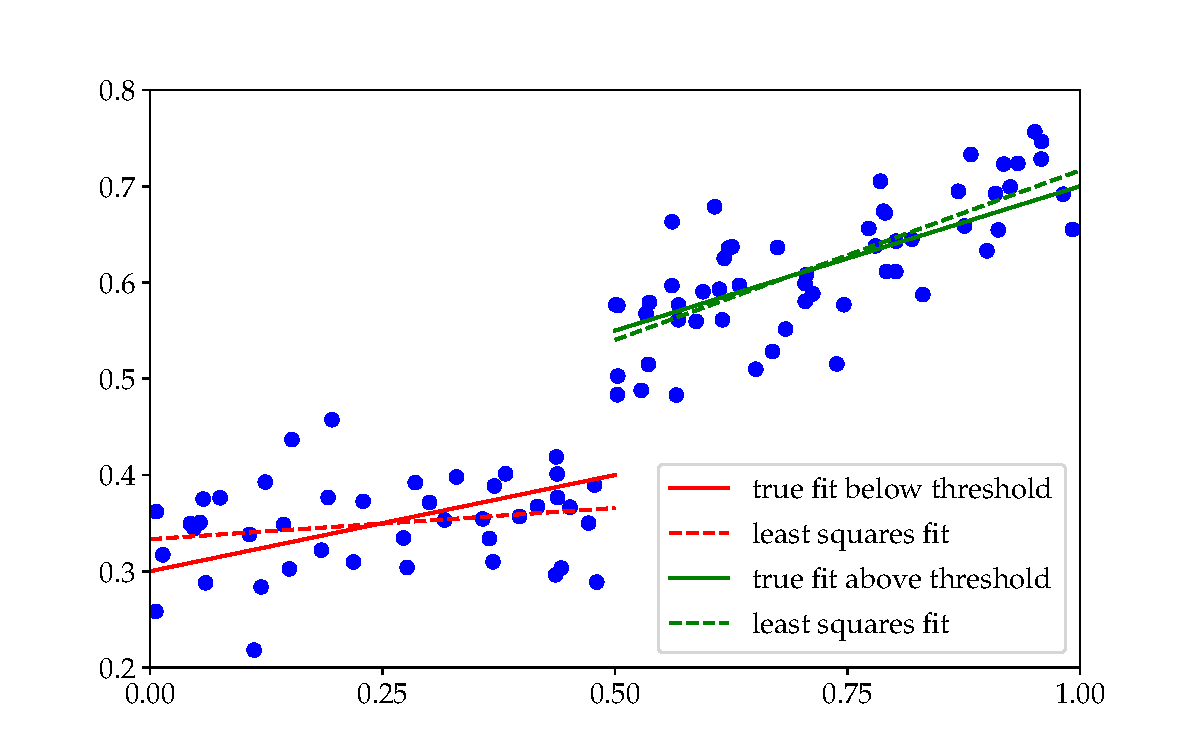
\includegraphics{assets/rdd}
\caption{Illustration of an idealized regression discontinuity. Real
examples are rarely this clear cut.}
\end{figure}

To illustrate the idea, consider an intervention in a hospital setting
that is assigned to newborn children just below a birth weight of 1500g.
We can ask if the intervention has a causal effect on wellbeing of the
child at a later age as reflected in an outcome variable, such as,
mortality or cumulative hospital cost in their first year. We expect
various factors to influence both birth weight and outcome variable. But
we hope that these confounding factors are essentially held constant
right around the threshold weight of 1500g. Regression discontinuity
designs have indeed been used to answer such questions for a number of
different outcome variables.\footnote{Almond et al., {``Estimating
  Marginal Returns to Medical Care: Evidence from at-Risk Newborns,''}
  \emph{The Quarterly Journal of Economics} 125, no. 2 (2010): 591--634;
  Bharadwaj, Løken, and Neilson, {``Early Life Health Interventions and
  Academic Achievement,''} \emph{American Economic Review} 103, no. 5
  (2013): 1862--91.}

Once we have identified the setup for a regression discontinuity, the
idea is to perform two regressions. One fits a model to the data below
the threshold. The other fits the model to data above the threshold. We
then take the difference of the values that the two models predict at
the threshold as our estimate of the causal effect. As usual, the idea
works out nicely in an idealized linear setting and can be generalized
in various ways.

There are numerous subtle and not so subtle ways a regression
discontinuity design can fail. One subtle failure mode is when
intervention incentivizes people to strategically make efforts to fall
just below or above the threshold. Manipulation or \emph{gaming} of the
running variable is a well-known issue for instance when it comes to
social program eligibility.\footnote{Camacho and Conover,
  {``Manipulation of Social Program Eligibility,''} \emph{American
  Economic Journal: Economic Policy} 3, no. 2 (2011): 41--65.} But there
are other less obvious cases. For example, school class sizes in data
from Chile exhibit irregularities that void regression discontinuity
designs.\footnote{Urquiola and Verhoogen, {``Class-Size Caps, Sorting,
  and the Regression-Discontinuity Design,''} \emph{American Economic
  Review} 99, no. 1 (2009): 179--215.} In turn, researchers have come up
with tests designed to catch such problems.

\hypertarget{instrumental-variables}{%
\subsection{Instrumental variables}\label{instrumental-variables}}

Instrumental variables are a popular quasi-experimental method for
causal inference. The starting point is confounding between a treatment
\(T\) and our outcome of interest~\(Y\). We are in a situation where
we're unable to resolve confounding via the adjustment formula. However,
what we have is the existence of a special variable~\(Z\) called an
\emph{instrument} that will help us estimate the treatment effect.

What makes~\(Z\) a valid instrument is nicely illustrated with the
following causal graph.

\begin{figure}
\centering
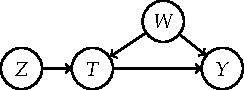
\includegraphics[width=0.5\textwidth,height=\textheight]{assets/causal-iv}
\caption{Typical graphical model for an instrumental variable setup}
\end{figure}

The graph structure encodes two key assumptions:

\begin{enumerate}
\def\labelenumi{\arabic{enumi}.}
\tightlist
\item
  The instrument \(Z\) and the outcome \(Y\) are unconfounded.
\item
  The instrument \(Z\) has no direct effect on the outcome \(Y\).
\end{enumerate}

Let's walk through how this works out in the one-dimensional linear
structural equation for the outcome: \[
Y= \alpha + \beta T + \gamma W + N
\] Here,~\(N\) is an independent noise term. For convenience, we denote
the \emph{error term} \(U=\gamma W + N\). What we're interested in is
the coefficient~\(\beta\) since we can easily verify that it corresponds
to the average treatment effect: \[
\beta = \mathop\mathbb{E}[Y\mid\mathrm{do}(T:=1)] - \mathop\mathbb{E}[Y\mid\mathrm{do}(T:=0)]
\] To find the coefficient~\(\beta,\) we cannot directly solve the
regression problem~\(Y=\alpha + \beta T + U\), because the error
term~\(U\) is not independent of~\(T\) due to the confounding influence
of~\(W\).

However, there's a way forward after we make a few additional
assumptions:

\begin{enumerate}
\def\labelenumi{\arabic{enumi}.}
\tightlist
\item
  The error term is zero mean: \(\mathop\mathbb{E}[U]=0\)
\item
  The instrument is uncorrelated with the error term:
  \(\mathop\mathrm{Cov}(Z, U)=0\)
\item
  Instrument and treatment have nonzero correlation:
  \(\mathop\mathrm{Cov}(Z, T)\ne 0\)
\end{enumerate}

The first two assumptions directly imply \[
\begin{aligned}
& \mathop\mathbb{E}[Y-\alpha-\beta T]= 0 \\
& \mathop\mathbb{E}[Z(Y-\alpha-\beta T)] = 0
\end{aligned}
\] This leaves us with two linear equations in~\(\alpha\) and~\(\beta\)
so that we can solve for both parameters. Indeed,
\(\alpha=\mathop\mathbb{E}[Y]-\beta\mathop\mathbb{E}[T]\). Plugging this
into the second equation, we have \[
\mathop\mathbb{E}[Z((Y-\mathop\mathbb{E}[Y])-\beta(T-\mathop\mathbb{E}[T]) )]=0,
\] which implies, via our third
assumption~\(\mathop\mathrm{Cov}(T, Z)\ne 0,\) \[
\beta = \frac{\mathop\mathrm{Cov}(Z, Y)}{\mathop\mathrm{Cov}(T, Z)}\,.
\] There's a different intuitive way to derive this solution by solving
a \emph{two step least squares} procedure:

\begin{enumerate}
\def\labelenumi{\arabic{enumi}.}
\tightlist
\item
  Predict the treatment from the instrument via least squares
  regression, resulting in the predictor \(\hat T = cZ\).
\item
  Predict the outcome from the predicted treatment using least squares
  regression, resulting in the predictor \(\hat Y=\beta' \hat T\).
\end{enumerate}

A calculation reveals that indeed~\(\beta'=\beta\), the desired
treatment effect. To see this note that \[
c=\frac{\mathop\mathrm{Cov}(Z, T)}{\mathop\mathrm{Var}(Z)}\,
\] and hence \[
\beta'
= \frac{\mathop\mathrm{Cov}(Y, \hat T)}{\mathop\mathrm{Var}(\hat T)}
= \frac{\mathop\mathrm{Cov}(Y, Z)}{c\mathop\mathrm{Var}(Z)}
= \frac{\mathop\mathrm{Cov}(Z, Y)}{\mathop\mathrm{Cov}(T, Z)}
= \beta\,.
\] This solution directly generalizes to the multi-dimensional linear
case. The two stage regression approach is in fact the way instrumental
variables is often introduced operationally. We see that again
instrumental variables is a clever way of reducing causal inference to
prediction.

One impediment to instrumental variables is a poor correlation between
the instrument and the treatment. Such instruments are called \emph{weak
instruments}. In this case, the
denominator~\(\mathop\mathrm{Cov}(T, Z)\) in our expression
for~\(\beta\) is small and the estimation problem is ill-conditioned.
The other impediment is that the causal graph corresponding to
instrumental variables is not necessarily easy to come by in
applications. What's delicate about the graph is that we want the
instrument to have a significant causal effect on the treatment, but at
the same time have no other causal powers that might influence the
outcome in a way that's not mediated by the treatment.

Nonetheless, researchers have found several intriguing applications of
instrumental variables. One famous example goes by the name \emph{judge
instruments}. The idea is that within the United States, at least in
certain jurisdictions and courts, defendants may be assigned randomly to
judges. Different judges then assign different sentences, some perhaps
more lenient, others harsher. The treatment here could be the sentence
length and the outcome may indicate whether or not the defendant went on
to commit another crime upon serving the prison sentence. A perfectly
random assignment of judges implies that the judge assignment and the
outcome are unconfounded. Moreover, the assignment of a judge has a
causal effect on the treatment, but plausibly no direct causal effect on
the outcome. The assignment of judges then serves as an instrumental
variable. The observation that judge assignments may be random has been
the basis of much causal inference about the criminal justice system.
However, the assumption of randomness in judge assignments has also been
challenged.\footnote{Chilton and Levy, {``Challenging the Randomness of
  Panel Assignment in the Federal Courts of Appeals,''} \emph{Cornell L.
  Rev.} 101 (2015): 1.}

\hypertarget{limitations-of-causal-inference-in-practice}{%
\section{Limitations of causal inference in
practice}\label{limitations-of-causal-inference-in-practice}}

It's worth making a distinction between causal modeling broadly speaking
and the practice of causal inference today. The previous chapter covered
the concepts of causal modeling. Structural causal models make it
painfully clear that the model necessarily specifies strong assumptions
about the data generating process. In contrast, the practice of causal
inference we covered in this chapter seems almost \emph{model-free} in
how it reduces to pattern classification via technical assumptions. This
appears to free the practitioner from difficult modeling choices.

The assumptions that make this all work, however, are not verifiable
from data. Some papers seek assurance in statistical robustness checks,
but these too are sample-based estimates. Traditional robustness checks,
such as resampling methods or leave-one-out estimates, may get at issues
of generalization, but cannot speak to the validity of causal
assumptions.

As a result, a certain pragmatic attitude has taken hold. If we cannot
verify the assumption from data anyway, we might as well make it in
order to move forward. But this is a problematic position. Qualitative
and theoretical ways of establishing substantive knowledge remain
relevant where the limitations of data set in. The validity of a causal
claim cannot be established solely based on a sample. Other sources of
substantive knowledge are required.

\hypertarget{validity-of-observational-methods}{%
\subsection{Validity of observational
methods}\label{validity-of-observational-methods}}

The empirical evidence regarding the validity of observational causal
inference studies is mixed and depends on the domain of application.

A well known article compared observational studies in the medical
domain between 1985 and 1998 to the results of randomized controlled
trials.\footnote{Benson and Hartz, {``A Comparison of Observational
  Studies and Randomized, Controlled Trials,''} \emph{New England
  Journal of Medicine} 342, no. 25 (2000): 1878--86.} The conclusion was
good news for observational methods:

\begin{quote}
We found little evidence that estimates of treatment effects in
observational studies reported after 1984 are either consistently larger
than or qualitatively different from those obtained in randomized,
controlled trials.
\end{quote}

Another study around the same time came to a similar conclusion:

\begin{quote}
The results of well-designed observational studies (with either a cohort
or a case--control design) do not systematically overestimate the
magnitude of the effects of treatment as compared with those in
randomized, controlled trials on the same topic.\footnote{Concato, Shah,
  and Horwitz, {``Randomized, Controlled Trials, Observational Studies,
  and the Hierarchy of Research Designs,''} \emph{New England Journal of
  Medicine} 342, no. 25 (2000): 1887--92.}
\end{quote}

One explanation, however, is that medical researchers may create
observational designs with great care on the basis of extensive domain
knowledge and prior investigation.

Freedman's paper \emph{Statistical Models and Shoe Leather} illustrates
this point through the famous example of Jon Snow's discovery from the
1850s that cholera is a waterborne disease.\footnote{Freedman,
  {``Statistical Models and Shoe Leather,''} \emph{Sociological
  Methodology}, 1991, 291--313.} Many associate Snow with an early use
of quantitative methods. But the application of those followed years of
substantive investigation and theoretical considerations that formed the
basis of the quantitative analysis.

In other domains, observational methods have been much less successful.
Online advertising, for example, generates hundreds of billions of
dollars in global revenue today, but the causal effects of targeted
advertising remain a subject of debate.\footnote{Hwang, \emph{Subprime
  Attention Crisis} (Farrar, Strauss; Giroux, 2020).} Randomized
controlled trials in this domain are rare for technical and cultural
reasons. Advertising platforms are highly optimized toward a particular
way of serving ads that can make true randomization difficult to
implement. As a result, practitioners rely on a range of observational
methods to determine the causal effect of showing and ad. However, these
methods tend to perform poorly as a recent large-scale study reveals:

\begin{quote}
The observational methods often fail to produce the same effects as the
randomized experiments, even after conditioning on extensive demographic
and behavioral variables. We also characterize the incremental
explanatory power our data would require to enable observational methods
to successfully measure advertising effects. Our findings suggest that
commonly used observational approaches based on the data usually
available in the industry often fail to accurately measure the true
effect of advertising.\footnote{Gordon et al., {``A Comparison of
  Approaches to Advertising Measurement: Evidence from Big Field
  Experiments at Facebook,''} \emph{Marketing Science} 38, no. 2 (2019):
  193--225.}
\end{quote}

\hypertarget{interference-interaction-and-spillovers}{%
\subsection{Interference, interaction, and
spillovers}\label{interference-interaction-and-spillovers}}

Confounding is not the only threat to the validity of causal studies. In
a medical setting, it's often relatively easy to ensure that treatment
of one subject does not influence the treatment assignment or outcome of
any other unit. We called this the Stable Unit Treatment Value
Assumption (SUTVA) in the previous chapter and noted that it holds by
default for the units in a structural causal models. Failures of SUTVA,
however, are common and go by many names, such as, interference,
interaction, and spill-over effects.

Take the example of an online social network. Interaction between units
is the default in all online platforms, whose entire purpose is that
people interact. Administering treatment to a subset of the platform's
users typically has some influence on the control group. For example, if
our treatment exposes a group of users to more content of a certain
kind, those users might share the content with others outside the
treatment group. In other words, treatment \emph{spills over} to the
control group. In certain cases, this problem can be mitigated by
assigning treatment to a cluster in the social network that has a
boundary with few outgoing edges thus limiting bias from
interaction.\footnote{Eckles, Karrer, and Ugander, {``Design and
  Analysis of Experiments in Networks: Reducing Bias from
  Interference,''} \emph{Journal of Causal Inference} 5, no. 1 (2016).}

Interference is also common in the economic development context. To
borrow an example from economist John Roemer,\footnote{Roemer, \emph{How
  We Cooperate: A Theory of Kantian Optimization} (Yale University
  Press, 2019).} suppose we want to know if better fishing nets would
improve the yield of fishermen in a town. We design a field experiment
in which we give better fishing nets to a random sample of fishermen.
The results show a significantly improved yield for the treated
fishermen. However, if we scale the intervention to the entire
population of fishermen, we might cause overfishing and hence reduced
yield for everyone.

\hypertarget{chapter-notes-9}{%
\section{Chapter notes}\label{chapter-notes-9}}

Aside from the introductory texts from the previous chapter, there are a
few more particularly relevant in the context of this chapter.

The textbook by Angrist and Pischke\footnote{Angrist and Pischke,
  \emph{Mostly Harmless Econometrics}.} covers causal inference with an
emphasis on regression analysis an applications in econometrics. See
Athey and Imbens\footnote{Athey and Imbens, {``The State of Applied
  Econometrics: Causality and Policy Evaluation,''} \emph{Journal of
  Economic Perspectives} 31, no. 2 (2017): 3--32.} for a more recent
survey of the state of causal inference in econometrics.

Marinescu et al.\footnote{Marinescu, Lawlor, and Kording,
  {``Quasi-Experimental Causality in Neuroscience and Behavioural
  Research,''} \emph{Nature Human Behaviour} 2, no. 12 (2018): 891--98.}
give a short introduction to quasi-experiments and their applications to
neuroscience with a focus on regression discontinuity design,
instrumental variables, and differences in differences.

\chapter{Sequential decision making and dynamic programming}

As the previous chapters motivated we don't just make predictions for
their own sake, but rather use data to inform decision making and
action. This chapter examines sequential decisions and the interplay
between predictions and actions in settings where our repeated actions
are directed towards a concrete end-goal. It will force us to understand
statistical models that evolve over time and the nature of dependencies
in data that is temporally correlated. We will also have to understand
feedback and its impact on statistical decision-making problems.

In machine learning, the subfield of using statistical tools to direct
actions in dynamic environments is commonly called ``reinforcement
learning'' (RL). However, this blanket term tends to lead people towards
specific solution techniques. So we are going to try to maintain a
higher view of the area of ``sequential decision making,'' including
perspectives from related fields of predictive analytics and optimal
control. These multiple perspectives will allow us to highlight how RL
is different from the machine learning we are most familiar
with.\index{reinforcement learning}

This chapter will follow a similar flow to our study of prediction. We
will formalize a temporal mathematical model of sequential decision
making involving notions from \emph{dynamical systems}. We will then
present a common optimization framework for making sequential decisions
when models are known: \emph{dynamic programming}. Dynamic programming
will enable algorithms for finding or approximating optimal decisions
under a variety of scenarios. In the sequel, we will turn to the
learning problem of how to best make sequential decisions when the
mechanisms underlying dynamics and costs are not known in
advance.\index{dynamic programming}

\hypertarget{from-predictions-to-actions}{%
\section{From predictions to
actions}\label{from-predictions-to-actions}}

Let's first begin with a discussion of how sequential decision making
differs from static prediction. In our study of decision theory, we laid
out a framework for making optimal predictions of a binary
covariate~\(Y\) when we had access to data~\(X\), and probabilistic
models of how~\(X\) and \(Y\) were related. Supervised learning was the
resulting problem of making such decisions from data rather than
probabilistic models.

In sequential decision making, we add two new variables. First, we
incorporate \emph{actions} denoted~\(U\) that we aim to take throughout
a procedure. We also introduce rewards~\(R\) that we aim to maximize. In
sequential decision making, the goal is to analyze the data~\(X\) and
then subsequently choose~\(U\) so that~\(R\) is large. We have explicit
agency in choosing~\(U\) and are evaluated based on some quality scoring
of~\(U\) and \(X\). There are an endless number of problems where this
formulation is applied from supply chain optimization to robotic
planning to online engagement maximization. Reinforcement learning will
be the resulting problem of making taking actions to maximize rewards
where our actions are only a function of previously observed data rather
than probabilistic models. Not surprisingly, the optimization problem
associated with sequential decision making is more challenging than the
one that arises in decision theory.

\hypertarget{dynamical-systems}{%
\section{Dynamical systems}\label{dynamical-systems}}

\index{dynamical system}

In addition to the addition to action variable in sequential decision
making, another key feature of sequential decision making problems is
the notion of time and sequence. We assume data is collected in an
evolving process, and our current actions influence our future rewards.

We begin by bringing all of these elements together in the general
definition of a discrete time dynamical system. The definitions both
simple and broad. We will illustrate with several examples shortly.

A \emph{dynamical system model} has a \emph{state} \(X_t\),
\emph{exogenous input} \(U_t\) modeling our \emph{control action}, and
\emph{reward} \(R_t\). The state evolves in discrete time steps
according to the equation \[
    X_{t+1} = f_t(X_t,U_t,W_t)
\] where~\(W_t\) is a random variable and~\(f_t\) is a function. The
reward is assumed to be a function of these variables as well: \[
    R_{t} = g_t(X_t,W_t)
\] for some function~\(g_t\). To simplify our notation throughout, we
will commonly write~\(R\) explicitly as a function of~\((X,U,W)\), that
is, \(R_t[X_t,U_t,W_t]\).

Formally, we can think of this definition as a structural equation model
that we also used to define causal models. After all, the equations
above give us a way to incrementally build up a data-generating process
from noise variables. Whether or not the dynamical system is intended to
capture any causal relationships in the real world is a matter of
choice. Practitioners might pursue this formalism for reward
maximization without modeling causal relationships. A good example is
the use of sequential decision making tools for revenue maximization in
targeted advertising. Rather than modeling causal relationships between,
say, preferences and clicks, targeted advertising heavily relies on all
sorts of signals, be they causal or not.

\hypertarget{concrete-examples}{%
\subsection{Concrete examples}\label{concrete-examples}}

\textbf{Grocery shopping.} Bob really likes to eat cheerios for
breakfast every morning. Let the state~\(X_t\) denotes the amount of
Cheerios in Bob's kitchen on day~\(t\). The action~\(U_t\) denotes the
amount of Cheerios Bob buys on day~\(t\) and~\(W_t\) denotes the amount
of Cheerios he eats that day. The random variable~\(W_t\) varies with
Bob's hunger. This yields the dynamical system \[
    X_{t+1} = X_t + U_t - W_t\,.
\] While this example is a bit cartoonish, it turns out that such simple
models are commonly used in managing large production supply chains. Any
system where resources are stochastically depleted and must be
replenished can be modeled comparably. If Bob had a rough model for how
much he eats in a given day, he could forecast when his supply would be
depleted. And he could then minimize the number of trips he'd need to
make to the grocer using optimal control.

\textbf{Moving objects.} Consider a physical model of a flying object.
The simplest model of the dynamics of this system are given by Newton's
laws of mechanics. Let~\(Z_t\) denote the position of the vehicle (this
is a three-dimensional vector). The derivative of position is velocity
\[
V_t = \frac{\partial Z_t}{\partial t}\,,
\] and the derivative of velocity is acceleration \[
A_t = \frac{\partial V_t}{\partial t}\,.
\] Now, we can approximate the rules in discrete time with the simple
Taylor approximations \[
\begin{aligned}
    Z_{t+1} &= Z_t + \Delta V_t\\
    V_{t+1} &= V_t + \Delta A_t
\end{aligned}
\] We also know by Newton's second law, that acceleration is equal to
the total applied force divided by the mass of the object:~\(F=mA\). The
flying object will be subject to external forces such as gravity and
wind~\(W_t\) and it will also receive forces from its
propellers~\(U_t\). Then we can add this to the equations to yield a
model \[
\begin{aligned}
    Z_{t+1} &= Z_t + \Delta V_t\\
    V_{t+1} &= V_t + \frac{\Delta}{m} (W_t+U_t)\,.
\end{aligned}
\]

Oftentimes, we only observe the acceleration through an accelerometer.
Then estimating the position and velocity becomes a filtering problem.
Optimal control problems for this model would including being able to
fly the object along a given trajectory or flying to a desired location
in a minimal amount of time.

\hypertarget{markov-decision-processes}{%
\subsection{Markov decision processes}\label{markov-decision-processes}}

\index{Markov decision process}

Our definition in terms of structural equations is not the only
dynamical model used in machine learning. Some people prefer to work
directly with probabilistic transition models and conditional
probabilities. In a \emph{Markov Decision Process}, we again have a
state \(X_t\) and input~\(U_t\), and they are linked by a probabilistic
model \[
    \mathop\mathbb{P}[X_{t+1}\mid X_t,U_t]\,.
\] This is effectively the same as the structural equation model above
except we hide the randomness in this probabilistic notation.

\textbf{Example: machine repair.} The following example illustrates the
elegance of the conditional probability models for dynamical systems.
This example comes from Bertsekas.\footnote{Bertsekas, \emph{Dynamic
  Programming and Optimal Control}, 4th ed., vol. 1 (Athena Scientific,
  2017).} Suppose we have a machine with ten states of repair. State 10
denotes excellent condition and 1 denotes the inability to function.
Every time one uses the machine in state~\(j\), it has a probability of
falling into disrepair, given by the
probabilities~\(\mathop\mathbb{P}[X_{t+1} = i\mid X_t=j]\,,\) where
\(\mathop\mathbb{P}[X_{t+1}=i\mid X_t=j]=0\) if~\(i>j\). The
action~\(a\) one can take at any time is to repair the machine,
resetting the system state to~\(10\). Hence \[
\mathop\mathbb{P}[X_{t+1}=i\mid X_{t}=j,U_t=0] = \mathop\mathbb{P}[X_{t+1}=i\mid X_{t}=j]
\] and \[
\mathop\mathbb{P}[X_{t+1}=i\mid X_{t}=j,U_t=1] = \mathbb{1}\left\{ i=10 \right\} \,.
\] While we could write this dynamical system as a structural equation
model, it is more conveniently expressed by these probability tables.

\hypertarget{optimal-sequential-decision-making}{%
\section{Optimal sequential decision
making}\label{optimal-sequential-decision-making}}

Just as risk minimization was the main optimization problem we studied
in static decision theory, there is an abstract class of optimization
problems that underlie most sequential decision making (SDM) problems.
The main problem is to find a sequence of decision \emph{policies} that
maximize a cumulative reward subject to the uncertain, stochastic system
dynamics. At each time, we assign a reward~\(R_t(X_t,U_t,W_t)\) to the
current state-action pair. The goal is to find a sequence of actions to
make the summed reward as large as possible: \[
\begin{array}{ll}
\text{maximize}_{\{u_t\}} & \mathop\mathbb{E}_{W_t}\left[ \sum_{t=0}^T R_t(X_t,u_t,W_t) \right]\\
\text{subject to} & X_{t+1} = f_t(X_t, u_t, W_t)\\
& \text{($x_0$ given)}
\end{array}
\] Here, the expected value is over the sequence of stochastic
disturbance variables~\(W_t\). Note here,~\(W_t\) is a random variable
and \(X_t\) are is hence also a random variable. The sequence of actions
\(\{u_t\}\) is our decision variable. It could be chosen via a random or
deterministic procedure as a matter of design. But it is important to
understand what information is allowed to be used in order to select
\(u_t\).

Since the dynamics are stochastic, the optimal SDM problem typically
allows a policy to observe the state before deciding upon the next
action. This allows a decision strategy to continually mitigate
uncertainty through feedback. This is why we optimize over policies
rather than over a deterministic sequence of actions. That is, our goal
is to find functions of the current state~\(\pi_t\) such that
\(U_t=\pi_t(X_t, X_{t-1}, \ldots)\) is optimal in expected value. By a
\emph{control policy} (or simply ``a policy'') we mean a function that
takes a trajectory from a dynamical system and outputs a new control
action. In order for~\(\pi_t\) to be implementable, it must only have
access only to previous states and actions.

The policies~\(\pi_t\) are the decision variables of the problem: \[
\begin{array}{ll}
\text{maximize}_{\pi_t} & \mathop\mathbb{E}_{W_t}\left[ \sum_{t=0}^T R_t(X_t,U_t,W_t) \right]\\
\text{subject to} & X_{t+1} = f(X_t, U_t, W_t) \\
& U_t = \pi_t(X_t, X_{t-1},\ldots)\\
& \text{($x_0$ given)}
\end{array}
\] Now,~\(U_t\) is explicitly a random variable as it is a function of
the state~\(X_t\).

This SDM problem will be the core of what we study in this chapter. And
our study will follow a similar path to the one we took with decision
theory. We will first study how to solve these SDM problems when we know
the model. There is a general purpose solution for these problems known
as \emph{dynamic programming}.

\hypertarget{dynamic-programming}{%
\section{Dynamic programming}\label{dynamic-programming}}

The dynamic programming solution to the SDM problem is based on the
\emph{principle of optimality}: if you've found an optimal control
policy for a time horizon of length~\(T\),~\(\pi_1,\ldots, \pi_T\), and
you want to know the optimal strategy starting at state~\(x\) at
time~\(t\), then you just have to take the optimal policy starting at
time~\(t\), \(\pi_t,\ldots,\pi_T\). The best analogy for this is based
on driving directions: if you have mapped out an optimal route from
Seattle to Los Angeles, and this path goes through San Francisco, then
you must also have the optimal route from San Francisco to Los Angeles
as the tail end of your trip. Dynamic programming is built on this
principle, allowing us to recursively find an optimal policy by starting
at the final time and going backwards in time to solve for the earlier
stages.\index{dynamic programming}

To proceed, define the \emph{Q-function} to be the
mapping\index{Q-function} \[
    \mathcal{Q}_{a\rightarrow b}(x,u) = \max_{\{u_t\}}\left\{ \mathop\mathbb{E}_{W_t}\left[ \sum_{t=a}^b R_t(X_t,u_t,W_t)\right] \,:\,X_{t+1} = f_t(X_t, u_t, W_t),\,(X_a,u_a)=(x,u)\right\}
\] The Q-function determines the best achievable value of the SDM
problem over times~\(a\) to~\(b\) when the action at time~\(a\) is set
to be \(u\) and the initial condition is~\(x\). It then follows that the
optimal value of the SDM problem is
\(\max_u \mathcal{Q}_{0\rightarrow T}(x_0,u)\), and the optimal policy
is \(\pi(x_0) = \arg \max_u \mathcal{Q}_{0\rightarrow T}(x_0,u)\). If we
had access to the Q-function for the horizon~\({0,T}\), then we'd have
everything we'd need to know to take the first step in the SDM problem.
Moreover, the optimal policy is only a function of the current state of
the system. Once we see the current state, we have all the information
we need to predict future states, and hence we can discard the previous
observations.

We can use dynamic programming to compute this Q-function and the
Q-function associated with every subsequent action. That is, clearly we
have that the terminal Q-function is \[
    \mathcal{Q}_{T\rightarrow T}(x,u) = \mathop\mathbb{E}_{W_T}\left[ R_T(x,u,W_T) \right]\,,
\] and then compute recursively \[
    \mathcal{Q}_{t\rightarrow T}(x,u) = \mathop\mathbb{E}_{W_t}\left[ R_t(x,u,W_t) +  \max_{u'} \mathcal{Q}_{t+1 \rightarrow T}(f_t(x,u,W_t),u')\right]\,.
\] This expression is known as Bellman's equation. We also have that for
all times~\(t\), the optimal policy is
\(u_t = \arg\max_u \mathcal{Q}_t (x_t,u)\) and the policy depends only
on the current state.

To derive this form of the Q-function, we assume inductively that this
form is true for all times beyond~\(t+1\) and then have the chain of
identities \[
\begin{aligned}
    \mathcal{Q}_{t\rightarrow T}(x,u) &= \max_{\pi_{t+1},\ldots,\pi_T} \mathop\mathbb{E}_{w}\left[R_t(x,u,W_t) +  \sum_{s=t+1}^T R_s(X_s,\pi_{s}(X_s),W_s)\right]\\
&=  \mathop\mathbb{E}_{W_t}\left[R_t(x,u,W_t) +  
\max_{\pi_{t+1},\ldots,\pi_T}\mathop\mathbb{E}_{W_{t+1},\ldots,W_T} \left\{
\sum_{s=t+1}^T R_s(X_s,\pi_{s}(X_s),W_s) \right\}\right]\\
 &=\mathop\mathbb{E}_{W_t}\left[R_t(x,u,W_t) +     \max_{\pi_{t+1}} Q\left\{f(x,u,W_t),\pi_{t+1}(f(x,u,W_t))\right\}\right]\\
 &= \mathop\mathbb{E}_{W_t}\left[R_t(x,u,W_t) +    \max_{u'} Q(f(x,u,W_t),u')\right]\,.
\end{aligned}
\] Here, the most important point is that the maximum can be exchanged
with the expectation with respect to the first~\(W_t\). This is because
the policies are allowed to make decisions based on the history of
observed states, and these states are deterministic functions of the
noise process.

\hypertarget{infinite-time-horizons-and-stationary-policies}{%
\subsection{Infinite time horizons and stationary
policies}\label{infinite-time-horizons-and-stationary-policies}}

The Q-functions we derived for these finite time horizons are \emph{time
varying}. One applies a different policy for each step in time. However,
on long horizons with time invariant dynamics and costs, we can get a
simpler formula. First, for example, consider the limit: \[
\begin{array}{ll}
\text{maximize} & \lim_{N\rightarrow \infty}  \mathop\mathbb{E}_{W_t}[ \frac{1}{N} \sum_{t=0}^N R(X_t,U_t,W_t) ]\\
\text{subject to} & X_{t+1} = f(X_t, U_t, W_t),~U_t=\pi_t(X_t)\\
& \text{($x_0$ given).}
\end{array}
\] Such infinite time horizon problems are referred to as \emph{average
cost} dynamic programs. Note that there are no subscripts on the rewards
or transition functions in this model.

Average cost dynamic programming is deceptively difficult. These
formulations are not directly amenable to standard dynamic programming
techniques except in cases with special structure. A considerably
simpler infinite time formulation is known as \emph{discounted} dynamic
programming, and this is the most popular studied formulation.
Discounting is a mathematical convenience that dramatically simplifies
algorithms and analysis. Consider the SDM problem \[
    \begin{array}{ll}
        \text{maximize} &  (1-\gamma) \mathop\mathbb{E}_{W_t}[ \sum_{t=0}^\infty \gamma^t R(X_t,U_t,W_t) ]\\
        \text{subject to} & X_{t+1} = f(X_t, U_t, W_t),~U_t=\pi_t(X_t)\\
        & \text{($x_0$ given).}
    \end{array}
\] where~\(\gamma\) is a scalar in~\((0,1)\) called the \emph{discount
factor}.\index{discount factor} For~\(\gamma\) close to~\(1\), the
discounted reward is approximately equal to the average reward. However,
unlike the average cost model, the discounted cost has particularly
clean optimality conditions. If we define~\(\mathcal{Q}_\gamma(x,u)\) to
be the Q-function obtained from solving the discounted problem with
initial condition~\(x\), then we have a discounted version of dynamic
programming, now with the same Q-functions on the left and right hand
sides: \[
    \mathcal{Q}_\gamma(x,u) = \mathop\mathbb{E}_{W} \left[ R(x,u,W) + \gamma  \max_{u'} \mathcal{Q}_\gamma(f(x,u,W),u')\right]\,.
\] The optimal policy is now for \emph{all times} to let \[
    u_t= \arg\max_u \mathcal{Q}_\gamma(x_t,u)\,.
\] The policy is time invariant and one can execute it without any
knowledge of the reward or dynamics functions. At every stage, one
simply has to maximize a function to find the optimal action.
Foreshadowing to the next chapter, the formula additionally suggest that
the amount that needs to be ``learned'' in order to ``control'' is not
very large for these infinite time horizon problems.

\hypertarget{computation}{%
\section{Computation}\label{computation}}

Though dynamic programming is a beautiful universal solution to the very
general SDM problem, the generality also suggests computationally
barriers. Dynamic programming is only efficiently solvable for special
cases, and we now describe a few important examples.

\hypertarget{tabular-mdps}{%
\subsection{Tabular MDPs}\label{tabular-mdps}}

Tabular MDPs refer to Markov Decision Processes with small number of
states and actions. Say that there are~\(S\) states and~\(A\) actions.
Then the the transition rules are given by tables of conditional
probabilities~\(\mathop\mathbb{P}[X_{t+1}|X_t,U_t]\), and the size of
such tables are \(S^2 A\). The Q-functions for the tabular case are also
tables, each of size~\(SA\), enumerating the cost-to-go for all possible
state action pairs.\index{tabular} In this case, the maximization \[
 \max_{u'}\mathcal{Q}_{a\rightarrow b}(x,u')
\] corresponds to looking through all of the actions and choosing the
largest entry in the table. Hence, in the case that the rewards are
deterministic functions of~\(x\) and~\(u\), Bellman's equation
simplifies to \[
    \mathcal{Q}_{t\rightarrow T}(x,u) = R_t(x,u) + \sum_{x'} \mathop\mathbb{P}[X_{t+1}=x'|X_t=x,U_t=u] \max_{u'} \mathcal{Q}_{t+1\rightarrow T}(x',u')\,.
\] This function can be computed by elementary matrix-vector operations:
the Q-functions are~\(S \times A\) arrays of numbers. The ``max''
operation can be performed by operating over each row in such an array.
The summation with respect to~\(x'\) can be implemented by multiplying a
\(SA \times S\) array by an~\(S\)-dimensional vector. We complete the
calculation by summing the resulting expression with the~\(S\times A\)
array of rewards. Hence, the total time to compute
\(\mathcal{Q}_{t\rightarrow T}\) is~\(O(S^2A)\).

\hypertarget{linear-quadratic-regulator}{%
\subsection{Linear quadratic
regulator}\label{linear-quadratic-regulator}}

The other important problem where dynamic programming is efficiently
solvable is the case when the dynamics are \emph{linear} and the rewards
are \emph{quadratic}. In control design, this class of problems is
generally referred to as the problem of the Linear Quadratic Regulator
(LQR):\index{linear quadratic regulator}\index{LQR} \[
\begin{array}{ll}
\text{minimize} \, & \mathop\mathbb{E}_{W_t} \left[\frac{1}{2}\sum_{t=0}^T X_t^T \Phi_t X_t + U_t^T \Psi_t U_t\right], \\
\text{subject to} & X_{t+1} = A_t X_t+ B_t U_t + W_t,~U_t=\pi_t(X_t) \\
& \text{($x_0$ given).}
\end{array}
\] Here,~\(\Phi_t\) and~\(\Psi_t\) are most commonly positive
semidefinite matrices.~\(w_t\) is noise with zero mean and bounded
variance, and we assume~\(W_t\) and~\(W_{t'}\) are independent
when~\(t\neq t'\). The state transitions are governed by a linear update
rule with~\(A_t\) and~\(B_t\) appropriately sized matrices. We also
abide by the common convention in control textbooks to pose the problem
as a minimization---not maximization---problem.

As we have seen above, many systems can be modeled by linear dynamics in
the real world. However, we haven't yet discussed cost functions. It's
important to emphasize here that cost functions are \emph{designed} not
given. Recall back to supervised learning: though we wanted to minimize
the number of errors made on out of sample data, on in sample data we
minimized convex surrogate problems. The situation is exactly the same
in this more complex world of dynamical decision making. Cost functions
are designed by the engineer so that the SDM problems are tractable but
also so that the desired outcomes are achieved. Cost function design is
part of the toolkit for online decision making, and quadratic costs can
often yield surprisingly good performance for complex problems.

Quadratic costs are also attractive for computational reasons. They are
convex as long as~\(\Phi_t\) and~\(\Psi_t\) are positive definite.
Quadratic functions are closed under minimization, maximization,
addition. And for zero mean noise~\(W_t\) with covariance~\(\Sigma\), we
know that the noise interacts nicely with the cost function. That is, we
have \[
    \mathbb{E}_W[(x+W)^T M (x+W)] = x^T M x + \operatorname{Tr}(Q\Sigma)
\] for any vector~\(x\) and matrix~\(M\). Hence, when we run dynamic
programming, every Q-function is necessarily quadratic. Moreover, since
the Q-functions are quadratic, the optimal action is a \emph{linear
function} of the state \[
    U_t = -K_t X_t
\] for some matrix~\(K_t\).

Now consider the case where there are static costs~\(\Phi_t=\Phi\) and
\(\Psi_t=\Psi\), and time invariant dynamics such that~\(A_t=A\)
and~\(B_t=B\) for all~\(t\). One can check that the Q-function on a
finite time horizon satisfies a recursion \[
 \mathcal{Q}_{t \rightarrow T}(x,u) = x^T \Phi x + u^T \Psi u + (Ax+Bu)^T M_{t+1} (Ax+Bu) + c_t\,.
\] for some positive definite matrix~\(M_{t+1}\). In the limit as the
time horizon tends to infinity, the optimal control \emph{policy} is
\emph{static, linear state feedback}: \[
    u_t = -K x_t\,.
\] \(K\) is defined by \[
    K=(\Psi + B^T M B)^{-1} B^T M A
\] and~\(M\) is a solution to the \emph{Discrete Algebraic Riccati
Equation}\index{Riccati Equation} \[
M = \Phi + A^T M A - (A^T M B)(\Psi + B^T M B)^{-1} (B^T M A)\,.
\] Here,~\(M\) is the unique solution of the Riccati equation where all
of the eigenvalues of~\(A-BK\) have magnitude less than~\(1\). Finding
this specific solution is relatively easy using standard linear
algebraic techniques. It is also the limit of the Q-functions computed
above.

\hypertarget{policy-and-value-iteration}{%
\subsection{Policy and value
iteration}\label{policy-and-value-iteration}}

Two of the most well studied methods for solving such discounted
infinite time horizon problems are \emph{value iteration} and
\emph{policy iteration}.\index{policy iteration}\index{value iteration}
Value iteration proceeds by the steps \[
    \mathcal{Q}_{k+1} (x,u) = \mathop\mathbb{E}_{W} \left[ R(x,u,W) + \gamma  \max_{u'} \mathcal{Q}_k (f(x,u,W),u')\right]\,.
\] That is, it simply tries to solve the Bellman equation by running a
fixed point operation. This method succeeds when the iteration is a
contraction mapping, and this occurs in many contexts.

On the other hand, Policy Iteration is a two step procedure:
\emph{policy evaluation} followed by \emph{policy improvement}. Given a
policy~\(\pi_k\), the policy evaluation step is given by \[
    \mathcal{Q}_{k+1} (x,u) = \mathop\mathbb{E} \left[  R(x,u,W) + \gamma \mathcal{Q}_k (f(x,\pi_k(x),W),u')\right]\,.
\] And then the policy is updated by the rule \[
    \pi_{k+1}(x) = \arg\max_u \mathcal{Q}_{k+1} (x,u)\,.
\] Often times, several steps of policy evaluation are performed before
updating the policy.

For both policy and value iteration, we need to be able to compute
expectations efficiently and must be able to update \emph{all values}
of~\(x\) and~\(u\) in the associated~\(Q\) functions. This is certainly
doable for tabular MDPs. For general low dimensional problems, policy
iteration and value iteration can be approximated by gridding state
space, and then treating the problem as a tabular one. Then, the
resulting~\(Q\) function can be extended to other~\((x,u)\) pairs by
interpolation. There are also special cases where the maxima and minima
yield closed form solutions and hence these iterations reduce to simpler
forms. LQR is a canonical example of such a situation.

\hypertarget{model-predictive-control}{%
\subsection{Model predictive control}\label{model-predictive-control}}

\index{model predictive control}

If the Q-functions in value or policy iteration converge quickly, it
suggests that very long term planning might not be necessary, and we can
effectively solve infinite horizon problem with short term planning.
This is the key idea behind one of the most powerful techniques for
efficiently and effectively finding quality policies for SDM problems
called \emph{model predictive control}.

Suppose that we aim to solve the infinite horizon average reward
problem: \[
\begin{array}{ll}
\text{maximize} & \lim_{T\rightarrow \infty} \mathop\mathbb{E}_{W_t}[\frac{1}{T}\sum_{t=0}^T R_t(W_t,U_t) ]\\
\text{subject to} & X_{t+1} = f_t(X_t, U_t, W_t)\\
& U_t = \pi_t(X_t)\\
& \text{($x_0$ given).}
\end{array}
\] Model Predictive Control computes an \emph{open loop} policy on a
finite horizon~\(H\) \[
\begin{array}{ll}
\text{maximize}_{u_t} & \mathop\mathbb{E}_{W_t}[ \sum_{t=0}^H R_t(X_t,u_t)]\\
\text{subject to} & X_{t+1} = f_t(X_t, u_t, W_t)\\
& \text{($X_0$ = x).}
\end{array}
\] This gives a sequence~\(u_0(x),\ldots, u_H(x)\). The policy is then
set to be~\(\pi(x)=u_0(x)\). After this policy is executed, we observe a
new state,~\(x'\), based on the dynamics. We then recompute the
optimization, now using~\(x_0=x'\) and setting the action to
be~\(\pi(x')= u_0(x')\).

MPC is a rather intuitive decision strategy. The main idea is to plan
out a sequence of actions for a given horizon, taking into account as
much uncertainty as possible. But rather than executing the entire
sequence, we play the first action and then gain information from the
environment about the noise. This direct feedback influences the next
planning stage. For this reason, model predictive control is often a
successful control policy even when implemented with inaccurate or
approximate models. Model Predictive Control also allows us to easily
add a variety of constraints to our plan at little cost, such as bounds
on the magnitude of the actions. We just append these to the
optimization formulation and then lean on the computational solver to
make us a plan with these constraints.

To concretely see how Model Predictive Control can be effective, it's
helpful to work through an example. Let's suppose the dynamics and
rewards are time invariant. Let's suppose further that the reward
function is bounded above, and there is some state-action pair
\((x_\star,u_\star)\) which achieves this maximal
reward~\(R_\mathrm{max}\).

Suppose we solve the finite time horizon problem where we enforce that
\((x,u)\) must be at~\((x_\star,u_\star)\) at the end of the time
horizon: \[
\begin{array}{ll}
\text{maximize} & \mathop\mathbb{E}_{W_t}[ \sum_{t=0}^H R(X_t,u_t)]\\
\text{subject to} & X_{t+1} = f(X_t, u_t, W_t)\\
& (X_H,U_H) = (x_\star,u_\star)\\
& \text{($X_0$ = x).}
\end{array}
\] We replan at every time step by solving this optimization problem and
taking the first action.

The following proposition summarizes how this policy performs

\begin{Proposition}

Assume that all rewards are bounded above by~\(R_{\mathrm{max}}\). Then
with the above MPC policy, we have for all~\(T\) that \[
 \mathbb{E}\left[ \frac{1}{T} \sum_{t=0}^T R(x_t,u_t)\right] \geq \frac{Q_{0\rightarrow H}(x_0,u_0)-H R_{\mathrm{max}}}{T}
 + \mathbb{E}_W[R(f(x_\star,u_\star,W),0)]\,.
\]

\end{Proposition}

The proposition asserts that there is a burn in cost associated with the
initial horizon length. This term goes to zero with~\(T\), but will have
different values for different~\(H\). The policy converges to a residual
average cost due to the stochasticity of the problem and the fact that
we try to force the system to the state~\((x_\star,u_\star)\).

\begin{Proof}

To analyze how the policy performs, we turn to Bellman's equation. For
any time~\(t\), the MPC policy is \[
    u_t = \arg\max_u \mathcal{Q}_{0\rightarrow H}(x_t,u)
\] Now, \[
    \mathcal{Q}_{0\rightarrow H}(x_t,u) = R(x_t,u) + \mathbb{E}[\max_{u'} \mathcal{Q}_{1\rightarrow H}(X_{t+1},u')]\,.
\]

Now consider what to do at the time~\(t+1\). A \emph{suboptimal}
strategy at this time is to try to play the optimal strategy on the
horizon \(1\rightarrow H\), and then do nothing on the last step. That
is, \[
\max_u \mathcal{Q}_{0\rightarrow H}(x_{t+1},u) \geq
                 \max_{u'} \mathcal{Q}_{1\rightarrow H}(x_{t+1},u') + \mathbb{E}[R(f(x_\star,u_\star,W_{t+H}),0)]\,.
\] The last expression follows because the action sequence from
\(1\rightarrow H\) enforces~\((x_{t+H},u_{t+H})=(x_\star,u_\star)\). The
first term on the right hand side was computed in expectation above,
hence we have \[
\mathbb{E}[\max_u \mathcal{Q}_{0\rightarrow H}(X_{t+1},u)] \geq
    \mathbb{E}[\mathcal{Q}_{0\rightarrow H}(x_t,u_t)] - \mathbb{E}[R(x_t,u_t,W)] + \mathbb{E}[R(f(x_\star,u_\star,W),0)] \,.
\] Unwinding this recursion, we find \[
\begin{aligned}
\mathbb{E}[\max_u \mathcal{Q}_{0\rightarrow H}(X_{T+1},u)] &\geq
    \mathcal{Q}_{0\rightarrow H}(x_0,u_0) - \mathbb{E}\left[\sum_{t=0}^T R(x_t,u_t,W_t)\right]\\
    &\qquad\qquad\qquad  + T \mathbb{E}[R(f(x_\star,u_\star,W),0)] \,.
    \end{aligned}
\] Since the rewards are bounded above, we can upper bound the left hand
side by~\(R_{\mathrm{max}} H\). Rearranging terms then proves the
theorem.

\end{Proof}

The main caveat with this argument is that there may not \emph{exist} a
policy that drives~\(x\) to~\(x_\star\) from an arbitrary initial
condition and any realization of the disturbance signal. Much of the
analysis of MPC schemes is devoted to guaranteeing that the problems are
\emph{recursively feasible}, meaning that such constraints can be met
for all time.

This example also shows how it is often helpful to have some sort of
recourse at the end of the planning horizon to mitigate the possibility
of greedy optimizing driving the system into a bad state. The terminal
condition of forcing~\(x_H=0\) adds an element of safety to the
planning, and ensures stable execution for all time. More general,
adding some terminal condition to the planning
horizon~\(\mathcal{C}(x_{H})\) is part of good Model Predictive Control
design and is often a powerful way to balance performance and
robustness.

\hypertarget{partial-observation-and-the-separation-heuristic}{%
\section{Partial observation and the separation
heuristic}\label{partial-observation-and-the-separation-heuristic}}

Let's now move to the situation where instead of observing the state
directly, we observe an output~\(Y_t\) instead: \[
    Y_t = h_t(X_t,U_t,W_t)\,.
\] All of the policies we derived from optimization formulations above
required feeding back a function of the state. When we can only act on
outputs, SDM problems are considerably more difficult.

\begin{enumerate}
\def\labelenumi{\arabic{enumi}.}
\item
  \textbf{Static Output Feedback is NP-hard} Consider the case of just
  building a static policy from the output~\(Y_t\). Let's suppose our
  model is just the simple linear model \[
  \begin{aligned}
   X_{t+1} &= A X_t + B U_t\\
   Y_t &= C X_t
  \end{aligned}
  \] here,~\(A\),~\(B\) and~\(C\) are matrices. Suppose we want to find
  a feedback policy~\(U_t = K Y_t\) ( where~\(K\) is a matrix) and all
  we want to guarantee is that for any initial~\(x_0\), the system state
  converges to zero. This problem is called \emph{static state feedback}
  and is surprisingly \emph{NP-Hard}. It turns out that the problem is
  equivalent to finding a matrix~\(K\) such that~\(A+BKC\) has all of
  its eigenvalues inside the unit circle in the complex
  plane.\footnote{Blondel and Tsitsiklis, {``A Survey of Computational
    Complexity Results in Systems and Control,''} \emph{Automatica} 36,
    no. 9 (2000): 1249--74.} Though in the MDP case, static state
  feedback was not only optimal, but computable for tabular MDPs and
  certain other SDM problems, static output feedback is computationally
  intractable.
\item
  \textbf{POMDPs are PSPACE hard.} Papadimitriou and Tsitsiklis showed
  that optimization of general POMDPs, even on small state spaces, was
  in all likelihood completely intractable.\footnote{Papadimitriou and
    Tsitsiklis, {``The Complexity of {M}arkov {D}ecision {P}rocesses,''}
    \emph{Mathematics of Operations Research} 12, no. 3 (1987): 441--50.}
  They reduced the problem of \emph{quantifier elimination} in logical
  satisfiability problems (QSAT) to POMDPs. QSAT seeks to determine the
  validity of statements like ``there exists \(x\) such that for all
  \(y\) there exists \(z\) such that for all \(w\) this logical formula
  is true.'' Optimal action in POMDPs essentially have to keep track of
  all of the possible true states that might have been visited given the
  partial observation and make actions accordingly. Hence, the policies
  have a similar flavor to quantifier elimination as they seek actions
  that are beneficial all possible occurrences of the unobserved
  variables. Since these policies act over long time horizons, the
  number of counterfactuals that must be maintained grows exponentially
  large.
\end{enumerate}

Despite these challenges, engineers solve POMDP problems all of the
time. Just because the problems are hard in general, doesn't mean they
are intractable on average. It only means that we cannot expect to have
``general purpose optimal algorithms'' for these problems. Fortunately,
suboptimal solutions are often times quite good for practice, and there
are many useful heuristics for decision making with partial information.
The most common approach to the output feedback problem is the following
two-stage strategy:

\begin{enumerate}
\def\labelenumi{\arabic{enumi}.}
\item
  \textbf{Filtering.} Using all of your past data~\(\{y_s\}\) for
  \(s=0,\ldots,t\), build an estimate,~\(\hat{x}_t\), of your state.
\item
  \textbf{Action based on certainty equivalence.} Solve the desired SDM
  problem as if you had perfect observation of the state~\(X_t\), using
  \(\hat{x}_t\) wherever you would have used an observation~\(X_t=x_t\).
  At run time, plug in the estimator~\(\hat{x}_t\) as if it were a
  perfect measurement of the state.
\end{enumerate}

This strategy uses a \emph{separation principle} between prediction and
action. For certain problems, this two-staged approach is actually
optimal. Notably, if the SDM problem has quadratic rewards/costs, if the
dynamics are linear, and if the noise process is Gaussian, then the
separation between prediction and action is optimal. More commonly, the
separation heuristic is suboptimal, but this abstraction also enables a
simple heuristic that is easy to debug and simple to
design.\index{separation principle}

While we have already covered algorithms for optimal control, we have
not yet discussed state estimation. Estimating the state of a dynamical
system receives the special name: \emph{filtering}.\index{filtering}
However, at the end of the day, filtering is a prediction problem.
Define the observed data up to time~\(t\) as \[
\tau_t := (y_t,\ldots, y_1, u_{t-1}, \ldots, u_1)\,.
\] The goal of filtering is to estimate a a function~\(h(\tau_t)\) that
predicts~\(X_t\). We now describe two approaches to filtering.

\hypertarget{optimal-filtering}{%
\subsection{Optimal filtering}\label{optimal-filtering}}

Given a model of the state transition function and the observation
function, we can attempt to compute the maximum \emph{a posteriori}
estimate of the state from the data. That is, we could
compute~\(p(x_t | \tau_t)\) and then estimate the mode of this density.
Here, we show that such an estimator has a relatively simple recursive
formula, though it is not always computationally tractable to compute
this formula.

To proceed, we first need a calculation that takes advantage of the
conditional independence structure of our dynamical system model. Note
that \[
\begin{aligned}
p(y_t, x_t, & x_{t-1}, u_{t-1} | \tau_{t-1} )
= \\
&p(y_t| x_t, x_{t-1}, u_{t-1}, \tau_{t-1} )
p(x_t | x_{t-1},u_{t-1}, \tau_{t-1} )\\
 &\qquad\qquad\qquad\qquad\times p(x_{t-1}|\tau_{t-1} )
p(u_{t-1}|\tau_{t-1} )\\
&= p(y_t| x_t )
p(x_t | x_{t-1},u_{t-1} )
p(x_{t-1}|\tau_{t-1} )
p(u_{t-1}|\tau_{t-1} )\,.
\end{aligned}
\] This decomposition is into terms we now recognize.
\(p(x_t | x_{t-1},u_{t-1} )\) and~\(p(y_t| x_t )\) define the POMDP
model and are known.~\(p(u_t|\tau_t)\) is our policy and it's what we're
trying to design. The only unknown here is~\(p(x_{t-1}|\tau_{t-1} )\),
but this expression gives us a recursive formula
to~\(p(x_{t}|\tau_{t} )\) for all \(t\).

To derive this formula, we apply Bayes rule and then use the above
calculation: \[
\begin{aligned}
p(x_t | \tau_t) &=\frac{\int_{x_{t-1}} p(x_t , y_t, x_{t-1}, u_{t-1} | \tau_{t-1}) }
                                                {\int_{x_t,x_{t-1}} p(x_t , y_t, x_{t-1}, u_{t-1}| \tau_{t-1})}\\
&=\frac{\int_{x_{t-1}} p(y_t| x_t ) p(x_t | x_{t-1},u_{t-1} )
p(x_{t-1}|\tau_{t-1} )
p(u_{t-1}|\tau_{t-1} ) }
{\int_{x_{t},x_{t-1}} p(y_t| x_t ) p(x_t | x_{t-1},u_{t-1} )
p(x_{t-1}|\tau_{t-1} )
p(u_{t-1}|\tau_{t-1} )}\\
&=\frac{\int_{x_{t-1}} p(y_t| x_t ) p(x_t | x_{t-1},u_{t-1} )
p(x_{t-1}|\tau_{t-1} ) }
{\int_{x_t,x_{t-1}} p(y_t| x_t ) p(x_t| x_{t-1},u_{t-1} )
p(x_{t-1}|\tau_{t-1} )}\,.\qquad (3)
\end{aligned}
\] Given a prior for~\(x_0\), this now gives us a formula to compute a
MAP estimate of~\(x_t\) for all~\(t\), incorporating data in a streaming
fashion. For tabular POMDP models with small state spaces, this formula
can be computed simply by summing up the conditional probabilities. In
POMDPs without inputs---also known as \emph{hidden markov models}---this
formula gives the forward pass of Viterbi's decoding algorithm. For
models where the dynamics are linear and the noise is Gaussian, these
formulas reduce into an elegant closed form solution known as
\emph{Kalman filtering}. In general, this optimal filtering algorithm is
called \emph{belief propagation} and is the basis of a variety of
algorithmic techniques in the field of graphical
models.\index{Kalman filtering}\index{belief propagation}

\hypertarget{kalman-filtering}{%
\subsection{Kalman filtering}\label{kalman-filtering}}

For the case of linear dynamical systems, the above calculation has a
simple closed form solution that looks similar to the solution of LQR.
This estimator is called a \emph{Kalman Filter}, and is one of the most
important tools in signal processing and estimation. The Kalman Filter
assumes a linear dynamical system driven by Gaussian noise with
observations corrupted by Gaussian noise \[
\begin{aligned}
 X_{t+1} &= A X_t+ B U_t + W_t\\
 Y_{t} & = C X_t + V_t\,.
\end{aligned}
\] Here, assume~\(W_t\) and~\(V_t\) are independent for all time and
Gaussian with means zero and covariances~\(\Sigma_W\) and~\(\Sigma_V\)
respectively. Because of the joint Gaussianity, we can compute a closed
form formula for the density of~\(X_t\) conditioned on the past
observations and actions,~\(p(x_t | \tau_t)\). Indeed,~\(X_t\) is a
Gaussian itself.

On an infinite time horizon, the Kalman Filter takes a simple and
elucidating form: \[
\begin{aligned}
    \hat{x}_{t+1} = A \hat{x}_t + B u_t - L (y_t - \hat{y}_t)\\
    \hat{y}_t = C \hat{x}_t
\end{aligned}
\] where \[
    L=A P C^T (C P C^T + \Sigma_V)^{-1}
\] and~\(P\) is the positive semidefinite solution to the discrete
algebraic Riccati equation \[
    P = A P A^T + \Sigma_W - (A P C^T) (CPC^T +\Sigma_V)^{-1} (C\Sigma A^T)\,.
\]

The derivation of this form follows from the calculation in Equation 3
But the explanation of the formulas tend to be more insightful than the
derivation. Imagine the case where~\(L=0\). Then our
estimate~\(\hat{x}_t\) simulates the same dynamics as our model with no
noise corruption. The matrix~\(L\) computes a correction for this
simulation based on the observed~\(y_t\). This feedback correction is
chosen in such a way such that~\(P\) is the steady state covariance of
the error~\(X_t-\hat{x}_t\).~\(P\) ends up being the minimum variance
possible with an estimator that is \emph{unbiased} in the sense that
\(\mathop\mathbb{E}[\hat{x}_t-X_t]=0\).

Another interesting property of this calculation is that the~\(L\)
matrix is the LQR gain associated with the LQR problem \[
\begin{array}{ll}
\text{minimize} \, & \lim_{T\rightarrow \infty}\mathop\mathbb{E}_{W_t} \left[\frac{1}{2}\sum_{t=0}^T X_t^T \Sigma_W X_t + U_t^T \Sigma_V U_t\right], \\
\text{subject to} & X_{t+1} = A^T X_t+ B^T U_t + W_t,~U_t=\pi_t(X_t) \\
& \text{($x_0$ given).}
\end{array}
\] Control theorists often refer to this pairing as the \emph{duality
between estimation and control}.

\hypertarget{feedforward-prediction}{%
\subsection{Feedforward prediction}\label{feedforward-prediction}}

While the optimal filter can be computed in simple cases, we often do
not have simple computational means to compute the optimal state
estimate. That said, the problem of state estimation is necessarily one
of prediction, and the first half of this course gave us a general
strategy for building such estimators from data. Given many simulations
or experimental measurements of our system, we can try to estimate a
function~\(h\) such that~\(X_t \approx h(\tau_t)\). To make this
concrete, we can look at \emph{time lags} of the history \[
\tau_{t-s\rightarrow t} := (y_t,\ldots, y_{t-s}, u_{t-1}, \ldots, u_{t-s})\,.
\] Such time lags are necessarily all the same length. Then estimating
\[
\begin{array}{ll}
\text{minimize}_h & \sum_t \operatorname{loss}(h(\tau_{t-s\rightarrow t}), x_t)
\end{array}
\] is a supervised learning problem, and standard tools can be applied
to design architectures for and estimate~\(h\).

\hypertarget{chapter-notes-10}{%
\section{Chapter notes}\label{chapter-notes-10}}

This chapter and the following chapter overlap significantly with a
survey of reinforcement learning by Recht,\footnote{Recht, {``A Tour of
  Reinforcement Learning: The View from Continuous Control,''}
  \emph{Annual Review of Control, Robotics, and Autonomous Systems} 2
  (2019).} which contains additional connections to continuous control.
Those further interested in learning more about continuous control from
an optimization viewpoint should consult the book by Borrelli et
al.\footnote{Borrelli, Bemporad, and Morari, \emph{Predictive Control
  for Linear and Hybrid Systems} (Cambridge University Press, 2017).}
This book also provides an excellent introduction to model predictive
control. Another excellent introduction to continuous optimal control
and filtering is Boyd's lecture notes.\footnote{Boyd, {``{Ee363}: Linear
  Dynamical Systems''} 2009.}

An invaluable introduction to the subject of dynamic programming is by
Bertsekas who has done pioneering research in this space and has written
some of the most well read texts.\footnote{Bertsekas, \emph{Dynamic
  Programming and Optimal Control}.} For the reader interested in a
mathematical introduction to dynamic programming on discrete processes,
we recommend Puterman's text.\footnote{Puterman, \emph{Markov Decision
  Processes: Discrete Stochastic Dynamic Programming}
  (Wiley-Interscience, 1994).} Puterman also explains the linear
programming formulation of dynamic programming.

\chapter{Reinforcement learning}

Dynamic programming and its approximations studied thus far all require
knowledge of the probabilistic mechanisms underlying how data and
rewards change over time. When these mechanisms are unknown, appropriate
techniques to probe and learn about the underlying dynamics must be
employed in order to find optimal actions. We shall refer to the
solutions to sequential decision making problems when the dynamics are
unknown as \emph{reinforcement learning.}\index{reinforcement learning}
Depending on context, the term may refer to a body of work in artificial
intelligence, the community of researchers and practitioners who apply a
certain set of tools to sequential decision making, and data-driven
dynamic programming. That said, it is a useful name to collect a set of
problems of broad interest to machine learning, control theory, and
robotics communities.

A particularly simple and effective strategy for reinforcement learning
problems is to estimate a predictive model for the dynamical system and
then to use the fit model as if it were the true model in the optimal
control problem. This is an application of the \emph{principle of
certainty equivalence}, an idea tracing back to the dynamic programming
literature of the 1950s.\footnote{Simon, {``Dynamic Programming Under
  Uncertainty with a Quadratic Criterion Function,''}
  \emph{Econometrica} 24, no. 1 (1956): 74--81; Theil, {``A Note on
  Certainty Equivalence in Dynamic Planning,''} \emph{Econometrica} 25,
  no. 2 (1957): 346--49.} Certainty equivalence is a general solution
strategy for the following problem. Suppose you want to solve some
optimization problem with a parameter~\(\vartheta\) that is unknown.
However, suppose we can gather data to estimate~\(\vartheta\). Then the
certainty equivalent solution is to use a point estimate
for~\(\vartheta\) as if it were the true value. That is, you act as if
you were certain of the value of~\(\vartheta\), even though you have
only estimated \(\vartheta\) from data. We will see throughout this
chapter that such certainty equivalent solutions are powerfully simple
and effective baseline for sequential decision making in the absence of
well specified models.\index{certainty equivalence}

Certainty equivalence is a very general principle. We can apply it to
the output of a filtering scheme that predicts state, as we described in
our discussion of partially observed Markov Decision Processes. We can
also apply this principle in the study of MDPs with unknown parameters.
For every problem in this chapter, our core baseline will always be the
certainty equivalent solution. Surprisingly, we will see that certainty
equivalent baselines are typically quite competitive and give a clear
illustration of the best quality one can expect in many reinforcement
learning problems.

\hypertarget{exploration-exploitation-tradeoffs-regret-and-pac-learning}{%
\section{Exploration-exploitation tradeoffs: Regret and PAC
learning}\label{exploration-exploitation-tradeoffs-regret-and-pac-learning}}

In order to compare different approaches to reinforcement learning, we
need to decide on some appropriate rules of comparison. Though there are
a variety of important metrics for engineering practice that must be
considered including ease of implementation and robustness, a
first-order statistical comparison might ask how many samples are needed
to achieve a policy with high reward.

For this question, there are two predominant conventions to compare
methods: \emph{PAC-error}\marginnote{PAC is a shorthand for
\emph{probably approximately correct}.} and \emph{regret}. PAC-error is
useful when we spend all of our time learning about a system, and then
want to know how suboptimal our solution will be when built from the
data gathered thus far. Regret is more geared towards online execution
where we evaluate the reward accrued at all time steps, even if we are
spending that time probing the system to learn about its dynamics. Our
focus in this chapter will be showing that these two concepts are
closely
related.\index{PAC}\index{probably approximately correct}\index{regret}

Let us formalize the two notions. As in the previous chapter, we will be
concerned with sequential decision making problems of the form \[
\begin{array}{ll}
\text{maximize}_{\pi_t} & \mathop\mathbb{E}_{W_t}\left[ \sum_{t=0}^T R_t(X_t,U_t,W_t) \right]\\
\text{subject to} & X_{t+1} = f(X_t, U_t, W_t) \\
& U_t = \pi_t(X_t, X_{t-1},\ldots)\\
& \text{($x_0$ given.)}
\end{array}
\] Let~\(\pi_\star\) denote the optimal policy of this problem.

For PAC, let's suppose we allocate~\(N\) samples to probe the system and
use them in some way to build a policy~\(\pi_N\). We can define the
optimization error of this policy to be \[
    \mathcal{E}(\pi_N)=\mathop\mathbb{E}\left[\sum_{t=1}^T R_t[X'_t,\pi_\star(X'_t),W_t]\right]-\mathop\mathbb{E}\left[\sum_{t=1}^T R_t[X_t,\pi_N(X_t),W_t]\right]\,.
\] Our model has~\((\delta,\epsilon)\)-PAC error if
\(\mathcal{E}(\pi_N)\leq \epsilon\) with probability at
least~\(1-\delta\). The probability here is measured with respect to the
sampling process and dynamics of the system.

Regret is defined similarly, but is subtly different. Suppose we are now
only allowed~\(T\) total actions and we want to understand the
cumulative award achieved after applying these~\(T\) actions. In this
case, we have to balance the number of inputs we use to find a good
policy (exploration) against the number of inputs used to achieve the
best reward (exploitation).

Formally, suppose we use a policy~\(\pi_t\) at each time step to choose
our action. Suppose~\(\pi_\star\) is some other fixed policy.
Let~\(X_t\) denote the states induced by the policy sequence~\(\pi_t\)
and~\(X_t'\) denote the states induced by~\(\pi_\star\). Then the
\emph{regret} of \(\{\pi_t\}\) is defined to be \[
    \mathcal{R}_T(\{\pi_t\}) = \mathop\mathbb{E}\left[\sum_{t=1}^T R_t[X'_t,\pi_\star(X'_t),W_t]\right]-\mathop\mathbb{E}\left[\sum_{t=1}^T R_t[X_t,\pi_t(X_t),W_t]\right]\,.
\] It is simply the expected difference in the rewards generated under
policy~\(\pi_\star\) as compared to those generated under policy
sequence \(\pi_t\). One major way that regret differs from PAC-error is
the policy can change with each time step.\index{regret}

One note of caution for both of these metrics is that they are comparing
to a policy~\(\pi_\star\). It's possible that the comparison policy
\(\pi_\star\) is not very good. So we can have small regret and still
not have a particularly useful solution to the SDM problem. As a
designer it's imperative to understand~\(\pi_\star\) to formalize the
best possible outcome with perfect information. That said, regret and
PAC-error are valuable ways to quantify how much exploration is
necessary to find nearly optimal policies. Moreover, both notions have
provided successful frameworks for algorithm development: many
algorithms with low regret or PAC-error are indeed powerful in practice.

\hypertarget{multi-armed-bandits}{%
\subsection{Multi-armed bandits}\label{multi-armed-bandits}}

The multi-armed bandit is one of the simplest reinforcement learning
problems, and studying this particular problem provides many insights
into exploration-exploitation
tradeoffs.\index{multi-armed bandits}\index{bandits}

In the multi-armed bandit, we assume \emph{no state whatsoever}. There
are \(K\) total actions, and the reward is a random function of which
action you choose. We can model this by saying there are i.i.d. random
variables~\(W_{t1},\ldots, W_{tk}\), and your reward is the dot product
\[
    R_t = [W_{t1},\ldots, W_{tK}] e_{u_t}
\] where~\(e_i\) is a standard basis vector. Here~\(W_{ti}\) take values
in the range~\([0,1]\). We assume that all of the~\(W_{ti}\) are
independent, and that~\(W_{ti}\) and~\(W_{si}\) are identically
distributed. Let \(\mu_{i} = \mathop\mathbb{E}[W_{ti}]\). Then the
expected reward at time~\(t\) is precisely~\(\mu_{u_t}\).

The multi-armed bandit problem is inspired by gambling on slot machines.
Indeed, a ``bandit'' is a colloquial name for a slot machine. Assume
that you have~\(K\) slot machines. Each machine has some probability of
paying out when you play it. You want to find the machine that has the
largest probability of paying out, and then play that machine for the
rest of time. The reader should take an opportunity to ponder the irony
that much of our understanding of statistical decision making comes from
gambling.

First let's understand what the optimal policy is if we know the model.
The total reward is equal to \[
    \mathop\mathbb{E}_{W_t}\left[ \sum_{t=0}^T R_t(u_t,W_t) \right] = \sum_{t=1}^T \mu_{u_t}\,.
\] The optimal policy is hence to choose a constant action~\(u_{t}=k\)
where~\(k = \arg\max_i \mu_i\).

When we don't know the model, it makes sense that our goal is to quickly
find the action corresponding to the largest mean. Let's first do a
simple PAC analysis, and then turn to the slightly more complicated
regret analysis. Our simple baseline is one of certainty equivalence. We
will try each action~\(N/K\) times, and compute the empirical return.
The empirical means are: \[
    \hat{\mu}_k = \frac{K}{N} \sum_{i=1}^{N/K} R_i^{(k)}
\] Our policy will be to take the action with the highest observed
empirical return.

To estimate the value of this policy, let's assume that the best action
is~\(u=1\). Then define \[
    \Delta_i  = \mu_1 -\mu_i\,.
\] Then we have \[
    \mathcal{E}(\pi_N) = \sum_{i=1}^K T \Delta_i \mathop\mathbb{P}[\forall i\colon \hat{\mu}_k \geq \hat{\mu}_i]\,.
\]

We can bound the probability that action~\(k\) is selected as follows.
First, if action~\(k\) has the largest empirical mean, it must have a
larger empirical mean than the true best option, action 1: \[
\mathop\mathbb{P}[\forall i\colon \hat{\mu}_k \geq \hat{\mu}_i]
\leq \mathop\mathbb{P}[ \hat{\mu}_k \geq \hat{\mu}_1]\,.
\] We can bound this last term using Hoeffding's inequality. Let
\(m=N/K\). Since each reward corresponds to an independent draw of some
random process, we have~\(\hat{\mu}_k - \hat{\mu}_1\) is the mean
of~\(2m\) independent random variables in the range~\([-1,1]\): \[
    \frac{1}{2} (\hat{\mu}_k - \hat{\mu}_1) =  \frac{1}{2m} \left( \sum_{i=1}^m R_i^{(k)} +\sum_{i=1}^m -R_i^{(1)} \right)\,.
\] Now writing Hoeffding's inequality for this random variable gives the
tail bound \[
\mathop\mathbb{P}[ \hat{\mu}_k \geq \hat{\mu}_1]
=\mathop\mathbb{P}[ \tfrac{1}{2}( \hat{\mu}_k- \hat{\mu}_1) \geq 0]
\leq \exp\left(-\frac{m\Delta_k^2}{4}\right)
\] which results in an optimization error \[
    \mathcal{E}(\pi_N) \leq \sum_{i=1}^K T \Delta_i \exp\left(-\frac{N\Delta_i^2}{4K}\right)\,.
\] with probability~\(1\). This expression reveals that the multi-armed
bandit problem is fairly simple. If~\(\Delta_i\) are all small, then any
action will yield about the same reward. But if all of the~\(\Delta_i\)
are large, then finding the optimal action only takes a few samples.
Naively, without knowing anything about the gaps at all, we can use the
fact that~\(x e^{-x^2/2}\leq \tfrac{1}{2}\) for nonnegative~\(x\) to
find \[
    \mathcal{E}(\pi_N) \leq \frac{K^{3/2} T}{\sqrt{N}}\,.
\] This shows that no matter what the gaps are, as long as~\(N\) is
larger than~\(K^3\), we would expect to have a high quality solution.

Let's now turn to analyzing regret of a simple certainty equivalence
baseline. Given a time horizon~\(T\), we can spend the first~\(m\) time
steps searching for the best return. Then we can choose this action for
the remaining~\(T-m\) time steps. This strategy is called
\emph{explore-then-commit}.\index{explore-then-commit}

The analysis of the explore-then-commit strategy for the multi-armed
bandit is a straightforward extension of the PAC analysis. If at round
\(t\), we apply action~\(k\), the expected gap between our policy and
the optimal policy is~\(\Delta_k\). So if we let~\(T_k\) denote the
number of times action~\(k\) is chosen by our policy then we must have
\[
    \mathcal{R}_T = \sum_{k=1}^K \mathop\mathbb{E}[T_k]\Delta_k\,.
\] \(T_k\) are necessarily random variables: what the policy learns
about the different means will depend on the observed sequence~\(x_k\)
which are all random variables.

Suppose that for exploration, we mimic our offline procedure, trying
each action~\(m\) times and record the observed rewards for that action
\(r_i^{(k)}\) for~\(i=1,\ldots,m\). At the end of these~\(mk\) actions,
we compute the empirical mean associated with each action as before.
Then we must have that \[
    \mathop\mathbb{E}[T_k] = m + (T-mK)\mathop\mathbb{P}[\forall i\colon \hat{\mu}_k \geq \hat{\mu}_i]\,.
\] The first term just states that each action is performed~\(m\) times.
The second term states that action~\(k\) is chosen for the commit phase
only if its empirical mean is larger than all of the other empirical
means.

Using Hoeffding's inequality again to bound these probabilities, we can
put everything together bound the expected regret as \[
 \mathcal{R}_T \leq \sum_{k=1}^K m\Delta_k + (T-mK) \Delta_k \exp\left(-\frac{m\Delta_k^2}{4}\right) \,.
\]

Let's specialize to the case of \emph{two} actions to see what we can
take away from this decomposition:

\begin{enumerate}
\def\labelenumi{\arabic{enumi}.}
\item
  \textbf{Gap dependent regret.} First, assume we know the gap between
  the means,~\(\Delta_2\), but we don't know which action leads to the
  higher mean. Suppose that \[
   m_0 = \left\lceil \frac{4}{\Delta_2^2} \log \left(\frac{T \Delta_2^2}{4} \right) \right\rceil \geq 1\,.
  \] Then using~\(m=m_0\), we have \[
  \begin{aligned}
   \mathcal{R}_T &\leq m\Delta_2 + T \Delta_2 \exp\left(-\frac{m\Delta_2^2}{4}\right)\\
   &\leq \Delta_2+ \frac{4}{\Delta_2} \left(\log \left(\frac{T \Delta_2^2}{4}\right)+1\right)\,.
  \end{aligned}
  \] If~\(m_0<1\), then~\(\Delta_2 <\frac{2}{\sqrt{T}}\), then choosing
  a random arm yields total expected regret at most \[
   \mathcal{R}_T = \frac{T}{2} \Delta_2 \leq \sqrt{T}\,.
  \] If~\(\Delta_2\) is very small, then we might also just favor the
  bound \[
   \mathcal{R}_T \leq \tfrac{1}{2}\Delta_2 T\,.
  \] Each of these bounds applies in different regimes and tells us
  different properties of this algorithm. The first bound shows that
  with appropriate choice of~\(m\), explore-then-commit incurs regret
  asymptotically bounded by~\(\log(T)\). This is effectively the
  smallest asymptotic growth achievable and is the gold standard for
  regret algorithms. However, this logarithmic regret bound depends on
  the gap~\(\Delta_2\). For small~\(\Delta_2\), the second bound shows
  the regret is never worse than~\(\sqrt{T}\) for any value of the gap.
  \(\sqrt{T}\) is one of the more common values for regret, and though
  it is technically asymptotically worse than logarithmic, algorithms
  with~\(\sqrt{T}\) regret tend to be more stable and robust than their
  logarithmic counterparts. Finally, we note that a very naive algorithm
  will incur regret that grows linearly with the horizon \(T\). Though
  linear regret is not typically an ideal situation, there are many
  applications where it's acceptable. If~\(\Delta_2\) is tiny to the
  point where it is hard to observe the difference between \(\mu_1\)
  and~\(\mu_2\), then linear regret might be completely satisfactory for
  an application.
\item
  \textbf{Gap independent regret.} We can get a gap
  independent,~\(\sqrt{T}\) regret for explore then commit for any value
  of~\(\Delta_2\). This just requires a bit of calculus: \[
  \begin{aligned}
  \frac{4}{\Delta_2} \left(\log \left(\frac{T \Delta^2}{4}\right)+1\right)
  & = 2\sqrt{T} \left( \frac{2}{\Delta_2\sqrt{T}} \left(\log \left(\frac{T \Delta^2}{4}\right)+1\right)   \right)\\
  & = 2\sqrt{T} \sup_{x\geq 0} \frac{2\log(x)+1}{x} \leq 4 e^{-1/2} \sqrt{T} \leq 2.5 \sqrt{T} \,.
  \end{aligned}
  \] Hence, \[
  \mathcal{R}_T \leq \Delta_2 + 2.5 \sqrt{T}
  \] no matter the size of~\(\Delta_2\) the gap is. Often times this
  unconditional bound is smaller than the logarithmic bound we derived
  above.
\item
  \textbf{Gap independent policy.} The stopping rule we described thus
  far requires knowing the value of~\(\Delta_2\). However, if we set
  \(m=T^{2/3}\) then we can achieve sublinear regret no matter what the
  value of~\(\Delta_2\) is. To see this again just requires some
  calculus: \[
  \begin{aligned}
  \mathcal{R}_T &\leq T^{2/3}\Delta_2 + T \Delta_2 \exp\left(-\frac{T^{2/3}\Delta_2^2}{4}\right)\\
  &= T^{2/3} \left(   \Delta_2 + T^{1/3} \Delta_2 \exp\left(-\frac{T^{2/3}\Delta_2^2}{4}\right)   \right)\\
  &\leq T^{2/3} \left(   \Delta_2 + 2 \sup_{x\geq 0} x e^{-x^2} \right) \leq 2 T^{2/3}\,.
  \end{aligned}
  \] \(O(T^{2/3})\) regret is technically ``worse'' than an asymptotic
  regret of~\(O(T^{1/2})\), but often times such algorithms perform well
  in practice. This is because there is a difference between worst case
  and average case behavior, and hence these worst-case bounds on regret
  themselves do not tell the whole story. A practitioner has to weigh
  the circumstances of their application to decide what sorts of
  worst-case scenarios are acceptable.
\end{enumerate}

\hypertarget{interleaving-exploration-and-exploitation}{%
\subsection{Interleaving exploration and
exploitation}\label{interleaving-exploration-and-exploitation}}

Explore-then-commit is remarkably simple, and illustrates most of the
phenomena associated with regret minimization. There are essentially two
main shortcomings in the case of the multi-armed bandit:

\begin{enumerate}
\def\labelenumi{\arabic{enumi}.}
\item
  For a variety of practical concerns, it would be preferable to
  interleave exploration with exploitation.
\item
  If you don't know the gap, you only get a~\(T^{2/3}\) rate.
\end{enumerate}

A way to fix this is called \emph{successive elimination}. As in
explore-then-commit, we try all actions~\(m\) times. Then, we drop the
actions that are clearly performing poorly. We then try the remaining
actions~\(4m\) times, and drop the poorly performing actions. We run
repeated cycles of this pruning procedure, yielding a collection of
better actions on average, aiming at convergence to the best return.
\index{successive elimination}

\begin{Algorithm}

\textbf{Successive Elimination Algorithm:}

\begin{itemize}
\tightlist
\item
  Given number of rounds \(B\) and an increasing sequence of positive
  integers \(\{m_\ell\}\).
\item
  Initialize the active set of options \(\mathcal{A}=\{1,\ldots,K\}\).
\item
  For \(\ell=1,\ldots, B\):

  \begin{enumerate}
  \def\labelenumi{\arabic{enumi}.}
  \tightlist
  \item
    Try every action in \(\mathcal{A}\) for \(m_\ell\) times.
  \item
    Compute the empirical means \(\hat{\mu}_k\) from this iteration
    only.
  \item
    Remove from \(\mathcal{A}\) any action \(j\) with
    \(\mu_j + 2^{-\ell} < \max_{k \in \mathcal{A}} \mu_k\).
  \end{enumerate}
\end{itemize}

\end{Algorithm}

The following theorem bounds the regret of successive elimination, and
was proven by Auer and Ortner.\footnote{Auer and Ortner, {``{UCB}
  Revisited: Improved Regret Bounds for the Stochastic Multi-Armed
  Bandit Problem,''} \emph{Periodica Mathematica Hungarica} 61, no. 1--2
  (2010): 55--65.}

\begin{Theorem}

With~\(B=\lfloor \tfrac{1}{2} \log_2 \tfrac{T}{e} \rfloor\) and
\(m_\ell = \lceil 2^{2\ell+1} \log \tfrac{T} {4^{\ell}} \rceil\), the
successive elimination algorithm accrues expected regret \[
\mathcal{R}_T \leq \sum_{i\colon\Delta_i > \lambda} \left( \Delta_i + \frac{32 \log(T\Delta_i^2) + 96}{\Delta_i} \right) + \max_{i\colon\Delta_i \leq \lambda} \Delta_i T
\] for any~\(\lambda>\sqrt{e/T}\).

\end{Theorem}

Another popular strategy is known as \emph{optimism in the face of
uncertainty}.\index{optimism} This strategy is also often called ``bet
on the best.'' At iteration~\(t\), take all of the observations seen so
far and form a set up upper confidence bounds~\(B_i\) such that \[
\mathop\mathbb{P}[\forall i\colon \mu_i \leq  B_i(t)] \leq 1-\delta
\] This leads to the Upper Confidence Bound (UCB)
algorithm.\index{upper confidence bound}\index{UCB}

\begin{Algorithm}

\textbf{UCB Algorithm}

\begin{itemize}
\tightlist
\item
  For \(t=1,\ldots, T\):

  \begin{enumerate}
  \def\labelenumi{\arabic{enumi}.}
  \tightlist
  \item
    Choose action \(k = \arg \max_i B_i(t-1)\).
  \item
    Play action \(k\) and observe reward \(r_t\).
  \item
    Update the confidence bounds.
  \end{enumerate}
\end{itemize}

\end{Algorithm}

For the simple case of the multi-armed bandit, we can use the bound that
would directly come from Hoeffding's inequality: \[
        B_i(t) = \hat{\mu}_i(t) + \sqrt{\frac{2 \log (1/\delta)}{T_i(t)}}
\] where we remind the reader that~\(T_i(t)\) denotes the number of
times we have tried action~\(i\) up to round~\(t\). Though~\(T_i(t)\) is
a random variable, one can still prove that this choice yields an
algorithm with nearly optimal regret.

More generally, optimistic algorithms work by maintaining an uncertainty
set about the dynamics model underlying the SDM problem. The idea is to
maintain a set~\(S\) where we have confidence our true model lies. The
algorithm then proceeds by choosing the model in~\(S\) which gives the
highest expected reward. The idea here is that either we get the right
model in which case we get a large reward, or we learn quickly that we
have a suboptimal model and we remove it from our set~\(S\).

\hypertarget{contextual-bandits}{%
\subsection{Contextual bandits}\label{contextual-bandits}}

\index{contextual bandits}

Contextual bandits provide a transition from multi-armed bandits to full
fledged reinforcement learning, introducing \emph{state} or
\emph{context} into the decision problem. Our goal in contextual bandits
is to iteratively update a policy to maximize the total reward: \[
    \text{maximize}_{u_t}~\mathop\mathbb{E}_{W_t}\left[\sum_{t=1}^T R(X_t,u_t,W_t)\right]
\] where we choose actions~\(u_t\) according to some policy that is a
function of the observations of the random variables~\(X_t\).
The~\(X_t\) are called \emph{contexts} or \emph{states} and we make no
assumptions about how they evolve over time. We assume that the reward
function is unknown and, at every time step, the received award is given
by \[
R(X_t,u_t,W_t)=R(X_t,u_t)+W_t
\] where~\(W_t\) is a random variable with zero mean and independent
from all other variables in the problem.

Contextual bandits are a convenient way to abstractly model engagement
problems on the internet. Every interaction a person has with the
website can be scored in term of some sort of reward function that
encodes information such as whether the person clicked, liked something,
or purchased an item. Whatever the reward function is, the goal will be
to maximize the total reward accumulated over all time. The~\(X_t\) will
be features describing the person's interaction history, and the action
will be related to the content served.

As was the case with the multi-armed bandit, the key idea in solving
contextual bandits is to reduce the problem to a prediction problem. In
fact we can upper bound our regret by our errors in prediction. The
regret accrued by a policy~\(\pi\) is \[
    \mathbb{E}\left\{\sum_{t=1}^T  \max_{u} R(X_t,u) - R(X_t, \pi(X_t)) \right\}\,.
\] This is because if we know the reward function, then the optimal
strategy is to choose the action that maximizes~\(R\). This is
equivalent to the dynamic programming solution when the dynamics are
trivial.

Let's reduce this problem to one of prediction. Suppose that at
time~\(t\) we have built an approximation of~\(R\),~\(\hat{R}_t(x,u)\).
Let's suppose that our algorithm uses the policy \[
    U_t = \arg \max_u \hat{R}_t(X_t,u)
\] That is, we take our current estimate as if it was the true reward,
and pick the action that maximizes reward given the context~\(X_t\).

To bound the regret for such an algorithm, note that we have for any
action~\(u\) \[
\begin{aligned}
    0 &\leq \hat{R}_t(X_t,\pi(X_t))-\hat{R}_t(X_t, u)\\
     &\leq R(X_t, \pi(X_t))-R(X_t, u) + (\hat{R}_t(X_t,\pi(X_t)) \\
     &\qquad\qquad- R(X_t, \pi(X_t) ))
     + (\hat{R}_t(X_t,u) - R(X_t, u ) )\,.   
\end{aligned}
\] Hence, \[
    \sum_{t=1}^T  \max_{u} R(X_t,u) - R(X_t, \pi(X_t))
    \leq 2 \sum_{t=1}^T \max_u | \hat{R}_t(X_t, u)-R(X_t, u)|\,.
\] This final inequality shows that if the prediction error goes to
zero, the associated algorithm accrues sublinear regret.

While there are a variety of algorithms for contextual bandits, we focus
our attention on two simple solutions that leverage the above reduction
to prediction. These algorithms work well in practice and are by far the
most commonly implemented. Indeed, they are so common that most
applications don't even call these implementations of contextual bandit
problems, as they take the bandit nature completely for granted.

This regret bound naturally suggests the following explore-then-commit
procedure.\index{explore-then-commit}

\begin{Algorithm}

\textbf{Explore-then-commit for contextual bandits}

\begin{itemize}
\tightlist
\item
  For \(t=1,2,\ldots, m\):

  \begin{enumerate}
  \def\labelenumi{\arabic{enumi}.}
  \tightlist
  \item
    Receive new context \(x_t\).
  \item
    Choose a random action \(u_t\).
  \item
    Receive reward \(r_t\).
  \end{enumerate}
\item
  Find a function to minimize prediction error:
  \(\textstyle\hat{R}_m~:=~\arg\min_f \sum_{s=1}^{m} \mathit{loss}(f(x_s,u_s),r_s)\,.\)
\item
  Define the policy \(\pi(x) = \arg\max_u \hat{R}_m(x_t,u)\).
\item
  for \(t=m+1,m+2,\ldots\):

  \begin{enumerate}
  \def\labelenumi{\arabic{enumi}.}
  \tightlist
  \item
    Receive new context \(x_t\).
  \item
    Choose the action given by \(\pi(x_t)\).
  \item
    Receive reward \(r_t\).
  \end{enumerate}
\end{itemize}

\end{Algorithm}

Second, an even more popular method is the following greedy
algorithm.\index{greedy algorithm}

\begin{Algorithm}

\textbf{Greedy algorithm for contextual bandits}

\begin{itemize}
\tightlist
\item
  For \(t=1,2,\ldots\)

  \begin{enumerate}
  \def\labelenumi{\arabic{enumi}.}
  \tightlist
  \item
    Find a function to minimize prediction error: \[
       \hat{R}_t := \arg\min_f \sum_{s=1}^{t-1}  \mathit{loss}(f(x_s,u_s),r_s) \,.
      \]
  \item
    Receive new context \(x_t\).
  \item
    Choose the action given by the policy \[
           \pi_t(x_t) := \arg\max_u \hat{R}_t(x_t,u) \,.
       \]
  \item
    Receive reward \(r_t\).
  \end{enumerate}
\end{itemize}

\end{Algorithm}

That industry has converged primarily on this one algorithm for a very
general problem is useful for many reasons. Though in worst case
settings, the greedy algorithm may accrue linear regret, Kannan et
al.~showed the algorithm performs well under mild assumptions about the
behavior of the client-base.\footnote{Kannan et al., {``A Smoothed
  Analysis of the Greedy Algorithm for the Linear Contextual Bandit
  Problem,''} in \emph{Advances in Neural Information Processing
  Systems}, 2018.} Essentially, only the most adversarial behavior can
cause the greedy algorithm to fail, and the greedy algorithm performs
perfectly fine on any slight random perturbation to this worst case
instance. Moreover, it is not always desirable to be exploring which
amounts to choosing random actions to see what happens. Empirically, the
value of adding exploration in practice seems limited at
best.\footnote{Hummel and McAfee, {``Machine Learning in an Auction
  Environment,''} \emph{Journal of Machine Learning Research} 17, no. 1
  (2016): 6915--51; Bietti, Agarwal, and Langford, {``A Contextual
  Bandit Bake-Off,''} \emph{arXiv:1802.04064}, 2018.} This context is
useful to keep in mind as we move to the more complex problem of
reinforcement learning and approximate dynamic programming.

\hypertarget{when-the-model-is-unknown-approximate-dynamic-programming}{%
\section{When the model is unknown: Approximate dynamic
programming}\label{when-the-model-is-unknown-approximate-dynamic-programming}}

We now bring dynamics back into the picture and attempt to formalize how
to solve general SDM problems when we don't know the dynamics model or
even the reward function. We turn to exploring the three main approaches
in this space: certainty equivalence fits a model from some collected
data and then uses this model as if it were true in the SDM problem.
Approximate Dynamic Programming uses Bellman's principle of optimality
and stochastic approximation to learn Q-functions from data. Direct
Policy Search directly searches for policies by using data from previous
episodes in order to improve the reward. Each of these has their
advantages and disadvantages as we now explore in depth.

\hypertarget{certainty-equivalence-for-sequential-decision-making}{%
\subsection{Certainty equivalence for sequential decision
making}\label{certainty-equivalence-for-sequential-decision-making}}

One of the simplest, and perhaps most obvious strategies to solve an SDM
problem when the dynamics are unknown is to estimate the dynamics from
some data and then to use this estimated model as if it were the true
model in the SDM problem.\index{certainty equivalence}

Estimating a model from data is commonly called ``system
identification'' in the dynamical systems and control literature. System
identification differs from conventional estimation because one needs to
carefully choose the right inputs to excite various degrees of freedom
and because dynamical outputs are correlated over time with the
parameters we hope to estimate, the inputs we feed to the system, and
the stochastic disturbances. Once data is collected, however,
conventional prediction tools can be used to find the system that best
agrees with the data and can be applied to analyze the number of samples
required to yield accurate models.

Let's suppose we want to build a predictor of the state~\(x_{t+1}\) from
the trajectory history of past observed states and actions. A simple,
classic strategy is simply to inject a random probing sequence~\(u_t\)
for control and then measure how the state responds. Up to stochastic
noise, we should have that \[
    x_{t+1} \approx \varphi(x_t,u_t) \,,
\] where~\(\varphi\) is some model aiming to approximate the true
dynamics.~\(\varphi\) might arise from a first-principles physical model
or might be a non-parametric approximation by a neural network. The
state-transition function can then be fit using supervised learning. For
instance, a model can be fit by solving the least-squares problem \[
\begin{array}{ll}
\text{minimize}_{\varphi} & \sum_{t=0}^{N-1} ||x_{t+1} - \varphi(x_t,u_t)||^2\,.
\end{array}
\]

Let~\(\hat{\varphi}\) denote the function fit to the collected data to
model the dynamics. Let~\(\omega_t\) denote a random variable that we
will use as a model for the noise process. With such a point estimate
for the model, we might solve the optimal control problem \[
\begin{array}{ll}
\text{maximize} & \mathop\mathbb{E}_{\omega_t}[ \sum_{t=0}^N R(x_t,u_t)  ]\\
\text{subject to} & x_{t+1} = \hat{\varphi}(x_t, u_t)+\omega_t,~u_t = \pi_t(\tau_t)\,.
\end{array}
\] In this case, we are solving the wrong problem to get our control
policies~\(\pi_t\). Not only is the model incorrect, but this
formulation requires some plausible model of the noise process. But we
emphasize that this is standard engineering practice. Though more
sophisticated techniques can be used to account for the errors in
modeling, feedback often can compensate for these modeling errors.

\hypertarget{approximate-dynamic-programming}{%
\subsection{Approximate dynamic
programming}\label{approximate-dynamic-programming}}

Approximate dynamic programming approaches the RL problem by directly
approximating the optimal control cost and then solving this with
techniques from dynamic programming. Approximate Dynamic Programming
methods typically try to Q-functions directly from data. The standard
assumption in most practical implementations of Q-learning is that the
Q-functions are static, as would be the case in the infinite horizon,
discounted optimal control problem.

Probably the best known approximate dynamic programming method is
\emph{Q-learning}.\footnote{Watkins and Dayan, {``Q-Learning,''}
  \emph{Machine Learning} 8, no. 3--4 (1992): 279--92.} Q-learning
simply attempts to solve value iteration using \emph{stochastic
approximation}.\index{Q-learning} If we draw a sample trajectory using
the policy given by the optimal policy, then we should have
(approximately and in expectation) \[
    \mathcal{Q}_\gamma(x_t,u_t) \approx R(x_t,u_t) + \gamma \max_{u'} \mathcal{Q}_\gamma(x_{t+1},u')\,.
\] Thus, beginning with some initial guess
\(\mathcal{Q}_\gamma^{(\mathrm{old})}\) for the Q-function, we can
update \[
    \mathcal{Q}_\gamma^{(\mathrm{new})}(x_t,u_t) = (1-\eta) \mathcal{Q}_\gamma^{(\mathrm{old})}(x_t,u_t) + \eta \left(R(x_t,u_t) + \gamma  \mathcal{Q}_\gamma^{(\mathrm{old})}(x_{t+1},u_{t+1})\right)
\] where~\(\eta\) is a \emph{step-size} or \emph{learning rate}.

The update here only requires data generated by the policy
\(Q_\gamma^{\mathrm{old}}\) and does not need to know the explicit form
of the dynamics. Moreover, we don't even need to know the reward
function if this is provided online when we generate trajectories.
Hence, Q-learning is often called ``model free.'' We strongly dislike
this terminology and do not wish to dwell on it. Unfortunately,
distinguishing between what is ``model-free'' and what is
``model-based'' tends to just lead to confusion. All reinforcement
learning is inherently based on models, as it implicitly assumes data is
generated by some Markov Decision Process. In order to run Q-learning we
need to know the form of the Q-function itself, and except for the
tabular case, how to represent this function requires \emph{some}
knowledge of the underlying dynamics. Moreover, assuming that value
iteration is the proper solution of the problem is a modeling
assumption: we are assuming a discount factor and time invariant
dynamics. But the reader should be advised that when they read
``model-free,'' this almost always means ``no model of the state
transition function was used when running this algorithm.''

For continuous control problems methods like Q-learning appear to make
an inefficient use of samples. Suppose the internal state of the system
is of dimension~\(d\). When modeling the state-transition function, each
sample provides~\(d\) pieces of information about the dynamics. By
contrast, Q-learning only uses~\(1\) piece of information per time step.
Such inefficiency is often seen in practice. Also troubling is the fact
that we had to introduce the discount factor in order to get a simple
form of the Bellman equation. One can avoid discount factors, but this
requires either considerably more sophisticated analysis. Large discount
factors do in practice lead to brittle methods, and the discount factor
becomes a hyperparameter that must be tuned to stabilize performance.

We close this section by noting that for many problems with high
dimensional states or other structure, we might be interested in not
representing Q-functions as a look up table. Instead, we might
approximate the Q-functions with a parametric family:
\(\mathcal{Q}(x,u;\vartheta)\). Though we'd like to update the parameter
\(\vartheta\) using something like gradient descent, it's not
immediately obvious how to do so. The simplest attempt, following the
guide of stochastic approximation is to run the iterations: \[
\begin{aligned}
\delta_t  &= R(x_{t},u_{t}) + \gamma  \mathcal{Q}(x_{t+1},u_{t+1}; \vartheta_{t})
- \mathcal{Q}(x_t,u_t;\vartheta_t)\\
\vartheta_{t+1} &= \vartheta_t + \eta \delta_t \nabla \mathcal{Q}(x_t,u_t,\vartheta_t)
\end{aligned}
\] This algorithm is called \emph{Q-learning with function
approximation}. A typically more stable version uses momentum to average
out noise in Q-learning. With~\(\delta_t\) as above, we add the
modification \[
\begin{aligned}
e_{t} &= \lambda e_{t-1} + \nabla \mathcal{Q}(x_t,u_t,\vartheta_t)\\
\vartheta_{t+1} &= \vartheta_t + \eta \delta_t e_t
\end{aligned}
\] for~\(\lambda \in [0,1]\). This method is known as
SARSA(\(\lambda\)).\footnote{Rummery and Niranjan, {``Online q-Learning
  Using Connectionist Systems''} (CUED/F-INFENG/TR 166, Cambridge
  University Engineering Dept., 1994).}

\hypertarget{direct-policy-search}{%
\subsection{Direct policy search}\label{direct-policy-search}}

The most ambitious form of control without models attempts to directly
learn a policy function from episodic experiences without ever building
a model or appealing to the Bellman equation. From the oracle
perspective, these policy driven methods turn the problem of RL into
derivative-free optimization.\index{policy search}

In turn, let's first begin with a review of a general paradigm for
leveraging random sampling to solve optimization problems. Consider the
general unconstrained optimization problem \[
\begin{array}{ll}
    \text{maximize}_{z\in\mathbb{R}^d} & R(z) \,.
    \end{array}
\] Any optimization problem like this is equivalent to an optimization
over probability densities on~\(z\): \[
\begin{array}{ll}
    \text{maximize}_{p(z)} & \mathbb{E}_p[R(z)] \,.
\end{array}
\] If~\(z_\star\) is the optimal solution, then we'll get the same value
if we put a~\(\delta\)-function around~\(z_\star\). Moreover, if~\(p\)
is a density, it is clear that the
\emph{expected value of the reward function} can never be larger than
the maximal reward achievable by a fixed~\(z\). So we can either
optimize over~\(z\) or we can optimize over \emph{densities} over \(z\).

Since optimizing over the space of all probability densities is
intractable, we must restrict the class of densities over which we
optimize. For example, we can consider a family parameterized by a
parameter vector~\(\vartheta\):~\(p(z;\vartheta)\) and attempt to
optimize \[
\begin{array}{ll}
    \text{maximize}_{\vartheta} & \mathbb{E}_{p(z;\vartheta)}[R(z)] \,.
\end{array}
\] If this family of densities contains all of the Delta functions, then
the optimal value will coincide with the non-random optimization
problem. But if the family does not contain the Delta functions, the
resulting optimization problem only provides a lower bound on the
optimal value no matter how good of a probability distribution we find.

That said, this reparameterization provides a powerful and general
algorithmic framework for optimization. In particular, we can compute
the derivative of~\(J(\vartheta):= \mathbb{E}_{p(z;\vartheta)}[R(z)]\)
using the following calculation (called ``the log-likelihood trick''):
\[
\begin{aligned}
    \nabla_{\vartheta} J(\vartheta) &= \int R(z) \nabla_{\vartheta} p(z;\vartheta) dz\\
    &= \int R(z) \left(\frac{\nabla_{\vartheta} p(z;\vartheta)}{p(z;\vartheta)}\right) p(z;\vartheta) dz\\
    &= \int \left( R(z) \nabla_{\vartheta} \log p(z;\vartheta) \right) p(z;\vartheta)dz \\
  &= \mathbb{E}_{p(z;\vartheta)}\left[ R(z) \nabla_{\vartheta} \log p(z;\vartheta) \right]\,.
\end{aligned}
\] This derivation reveals that the gradient of~\(J\) with respect to
\(\vartheta\) is the expected value of the function \[
    G(z,\vartheta) = R(z) \nabla_{\vartheta} \log p(z;\vartheta)
\] Hence, if we sample~\(z\) from the distribution defined by
\(p(z;\vartheta)\), we can compute~\(G(z,\vartheta)\) and will have an
unbiased estimate of the gradient of~\(J\). We can follow this direction
and will be running stochastic gradient descent on~\(J\), defining the
following algorithm:\index{REINFORCE}

\begin{Algorithm}

\textbf{REINFORCE algorithm:}

\begin{itemize}
\tightlist
\item
  \emph{Input Hyperparameters:} step-sizes \(\alpha_j>0\).
\item
  \emph{Initialize:} \(\vartheta_0\) and \(k = 0\).
\item
  Until the heat death of the universe, do:

  \begin{enumerate}
  \def\labelenumi{\arabic{enumi}.}
  \tightlist
  \item
    Sample \(z_k\sim p(z;\vartheta_k)\).
  \item
    Set
    \(\vartheta_{k+1} = \vartheta_k + \alpha_k R(z_k) \nabla_\vartheta \log p(z_k; \vartheta_k)\).
  \item
    \(k\leftarrow k + 1\).
  \end{enumerate}
\end{itemize}

\end{Algorithm}

The main appeal of the REINFORCE Algorithm is that it is trivial to
implement. If you can efficiently sample from~\(p(z;\vartheta)\) and can
easily compute~\(\nabla \log p\), you can run this algorithm on
essentially any problem. But such generality must and does come with a
significant cost. The algorithm operates on stochastic gradients of the
sampling distribution, but the function we cared about
optimizing---\(R\)---is only accessed through function evaluations.
Direct search methods that use the log-likelihood trick are necessarily
derivative free optimization methods, and, in turn, are necessarily less
effective than methods that compute actual gradients, especially when
the function evaluations are noisy. Another significant concern is that
the choice of distribution can lead to very high variance in the
stochastic gradients. Such high variance in turn implies that many
samples need to be drawn to find a stationary point.

That said, the ease of implementation should not be readily discounted.
Direct search methods are trivial to implement, and oftentimes
reasonable results can be achieved with considerably less effort than
custom solvers tailored to the structure of the optimization problem.
There are two primary ways that this sort of stochastic search arises in
reinforcement learning: Policy gradient and pure random search.

\hypertarget{policy-gradient}{%
\subsection{Policy gradient}\label{policy-gradient}}

Though we have seen that the optimal solutions of Bellman's equations
are deterministic, probabilistic policies can add an element of
exploration to a control strategy, hopefully enabling an algorithm to
simultaneously achieve reasonable awards and learn more about the
underlying dynamics and reward functions. Such policies are the starting
point for \emph{policy gradient}
methods.\footnote{Williams, {``Simple Statistical Gradient-Following
  Algorithms for Connectionist Reinforcement Learning,''} \emph{Machine
  Learning} 8, no. 3--4 (1992): 229--56.}\index{policy gradient}

Consider a \emph{parametric, randomized policy} such that~\(u_t\) is
sampled from a distribution~\(p(u \vert \tau_t;\vartheta)\) that is only
a function of the currently observed trajectory and a parameter vector
\(\vartheta\). A probabilistic policy induces a probability distribution
over trajectories: \[
    p(\tau;\vartheta) = \prod_{t=0}^{L-1} p(x_{t+1} \vert x_{t},u_{t}) p(u_t \vert \tau_t ;\vartheta)\,.
\] Moreover, we can overload notation and define the reward of a
trajectory to be \[
    R(\tau) = \sum_{t=0}^N R_t(x_t,u_t)
\] Then our optimization problem for reinforcement learning takes the
form of stochastic search. Policy gradient thus proceeds by sampling a
trajectory using the probabilistic policy with
parameters~\(\vartheta_k\), and then updating using REINFORCE.

Using the log-likelihood trick and the factored form of the probability
distribution~\(p(\tau;\vartheta)\), we can see that the gradient
of~\(J\) with respect to~\(\vartheta\) \emph{is not a function of the
underlying dynamics}. However, at this point this should not be
surprising: by shifting to distributions over policies, we push the
burden of optimization onto the sampling procedure.

\hypertarget{pure-random-search}{%
\subsection{Pure random search}\label{pure-random-search}}

\index{random search}

An older and more widely applied method to solve the generic stochastic
search problem is to directly perturb the current decision
variable~\(z\) by random noise and then update the model based on the
received reward at this perturbed value. That is, we apply the REINFORCE
Algorithm with sampling
distribution~\(p(z;\vartheta) = p_0(z-\vartheta)\) for some
distribution~\(p_0\). Simplest examples for~\(p_0\) would be the uniform
distribution on a sphere or a normal distribution. Perhaps less
surprisingly here, REINFORCE can again be run without any knowledge of
the underlying dynamics. The REINFORCE algorithm has a simple
interpretation in terms of gradient approximation. Indeed, REINFORCE is
equivalent to approximate gradient ascent of~\(R\) \[
    \vartheta_{t+1} = \vartheta_{t} + \alpha g_\sigma(\vartheta_k)
\] with the gradient approximation \[
    g_\sigma(\vartheta) = \frac{R(\vartheta + \sigma \epsilon) - R(\vartheta - \sigma \epsilon) }{2\sigma} \epsilon\,.
\] This update says to compute a finite difference approximation to the
gradient along the direction~\(\epsilon\) and move along the gradient.
One can reduce the variance of such a finite-difference estimate by
sampling along multiple random directions and averaging: \[
    g^{(m)}_\sigma(\vartheta) = \frac{1}{m} \sum_{i=1}^m\frac{R(\vartheta + \sigma \epsilon_i) - R(\vartheta - \sigma \epsilon_i) }{2\sigma} \epsilon_i\,.
\] This is akin to approximating the gradient in the random subspace
spanned by the~\(\epsilon_i\)

This particular algorithm and its generalizations goes by many different
names. Probably the earliest proposal for this method is
Rastrigin.\footnote{Rastrigin, {``About Convergence of Random Search
  Method in Extremal Control of Multi-Parameter Systems.''}
  \emph{Avtomat. I Telemekh.} 24, no. 11 (1963): 1467---1473.} Somewhat
surprisingly, Rastrigin initially developed this method to solve
reinforcement learning problems. His main motivating example was an
inverted pendulum. A rigorous analysis using contemporary techniques was
provided by Nesterov and Spokoiny.\footnote{Nesterov and Spokoiny,
  {``Random Gradient-Free Minimization of Convex Functions,''}
  \emph{Foundations of Computational Mathematics} 17, no. 2 (2017):
  527--66.} Random search was also discovered by the evolutionary
algorithms community and is called \((\mu,\lambda)\)-Evolution
Strategies.\footnote{Beyer and Schwefel, {``{Evolution Strategies} - a
  Comprehensive Introduction,''} \emph{Natural Computing} 1, no. 1
  (2002): 3--52; Schwefel, {``Evolutionsstrategie Und Numerische
  Optimierung''} (TU Berlin, 1975).} Random search has also been studied
in the context of stochastic approximation\footnote{Spall,
  {``Multivariate Stochastic Approximation Using a Simultaneous
  Perturbation Gradient Approximation,''} \emph{Transactions on
  Automatic Control} 37, no. 3 (1992): 332--41.} and bandits.\footnote{Flaxman,
  Kalai, and McMahan, {``Online Convex Optimization in the Bandit
  Setting: Gradient Descent Without a Gradient,''} in \emph{Symposium on
  Discrete Algorithms} (Society for Industrial; Applied Mathematics,
  2005), 385--94; Agarwal, Dekel, and Xiao, {``Optimal Algorithms for
  Online Convex Optimization with Multi-Point Bandit Feedback,''} in
  \emph{Conference on Learning Theory}, 2010.} Algorithms that get
invented by four different communities probably have something good
going for them.

\hypertarget{deep-reinforcement-learning}{%
\subsection{Deep reinforcement
learning}\label{deep-reinforcement-learning}}

\index{deep reinforcement learning}\index{reinforcement learning!deep}

We have thus far spent no time discussing \emph{deep} reinforcement
learning. That is because there is nothing conceptually different other
than using neural networks for function approximation. That is, if one
wants to take any of the described methods and make them deep, they
simply need to add a neural net. In model-based RL,~\(\varphi\) is
parameterized as a neural net, in ADP, the Q-functions or Value
Functions are assumed to be well-approximated by neural nets, and in
policy search, the policies are set to be neural nets. The algorithmic
concepts themselves don't change. However, convergence analysis
certainly will change, and algorithms like Q-learning might not even
converge. The classic text Neurodynamic Programming by Bertsekas and
Tsitisklis discusses the adaptations needed to admit function
approximation.\footnote{Bertsekas and Tsitsiklis, \emph{Neuro-Dynamic
  Programming} (Athena Scientific, 1996).}

\hypertarget{certainty-equivalence-is-often-optimal-for-reinforcement-learning}{%
\section{Certainty equivalence is often optimal for reinforcement
learning}\label{certainty-equivalence-is-often-optimal-for-reinforcement-learning}}

In this section, we give a survey of the power of certainty equivalence
in sequential decision making problems. We focus on the simple cases of
tabular MDPs and LQR as they are illustrative of more general problems
while still being manageable enough to analyze with relatively simple
mathematics. However, these analyses are less than a decade old. Though
the principle of certainty equivalence dates back over 60 years, our
formal understanding of certainty equivalence and its robustness is just
now solidifying.

\hypertarget{certainty-equivalence-for-lqr}{%
\subsection{Certainty equivalence for
LQR}\label{certainty-equivalence-for-lqr}}

\index{linear quadratic regulator}

Consider the linear quadratic regulator problem \[
\begin{array}{ll}
\text{minimize} \, & \lim_{T\rightarrow \infty} \mathop\mathbb{E}_{W_t} \left[\frac{1}{2T}\sum_{t=0}^T X_t^T\Phi X_t + U_t^T \Psi U_t\right], \\
\text{subject to} & X_{t+1} = A X_t+ B U_t + W_t,~U_t=\pi_t(X_t) \\
& \text{($x_0$ given).}
\end{array}
\] We have shown that the solution to this problem is static state
feedback~\(U_t = -K_\star X_t\) where \[
    K_\star=(\Psi + B^T M B)^{-1} B^T M A
\] and~\(M\) is the unique stabilizing solution to the Discrete
Algebraic Riccati Equation \[
M = \Phi + A^T M A - (A^T M B)(\Psi + B^T M B)^{-1} (B^T M A)\,.
\]

Suppose that instead of knowing~\((A,B,\Phi,\Psi)\) exactly, we only
have estimates~\((\hat{A},\hat{B},\hat{\Phi},\hat{\Psi})\). Certainty
equivalence would then yield a control policy~\(U_t = -\hat{K} X_t\)
where \(\hat{K}\) can be found
using~\((\hat{A},\hat{B},\hat{\Phi},\hat{\Psi})\) in place
of~\((A,B,\Phi,\Psi)\) in the formulae above. What is the cost of this
model?

The following discussion follows arguments due to Mania et
al.\footnote{Mania, Tu, and Recht, {``Certainty Equivalence Is Efficient
  for Linear Quadratic Control,''} in \emph{Advances in Neural
  Information Processing Systems}, 2019.} Let~\(J(K)\) denote that cost
of using the policy~\(K\). Note that this cost may be infinite, but it
will also be differentiable in~\(K\). If we unroll the dynamics and
compute expected values, one can see that the cost is the limit of
polynomials in~\(K\), and hence is differentiable.

Suppose that \[
    \epsilon := \max \left\{ \|\hat{A}-A\|,\, \|\hat{B}-B\|,\, \|\hat{\Phi}-\Phi\|,\, \|\hat{\Psi}-\Psi\|\right\}
\] If we Taylor expand the cost we find that for some~\(t \in [0,1]\),
\[
    J(\hat{K})-J_\star = \langle \nabla J(K_\star), \hat{K}-K_\star \rangle + \frac{1}{2} (\hat{K}-K_\star)^T \nabla^2 J(\tilde{K})(\hat{K}-K_\star)\,.
\] where~\(\tilde{K} = (1-t)K_\star + t \hat{K}\). The first term is
equal to zero because~\(K_\star\) is optimal. Since the map from
\((A,B,\Phi,\Psi)\) to~\(K_\star\) is differentiable, there must be
constants~\(L\) and~\(\epsilon_0\) such that
\(\|\hat{K}-K_\star\| \leq L \epsilon\) whenever
\(\epsilon \leq \epsilon_0\). This means that as long as the estimates
for \((A,B,\Phi,\Psi)\) are close enough to the true values, we must
have \[
    J(\hat{K})-J_\star = O(\epsilon^2)\,.
\]

Just how good should the estimates for these quantities be? Let's focus
on the dynamics~\((A,B)\) as the cost matrices~\(\Phi\) and~\(\Psi\) are
typically design parameters, not unknown properties of the system.
Suppose~\(A\) is~\(d\times d\) and~\(B\) is~\(d\times p\). Basic
parameter counting suggests that if we observe~\(T\) sequential states
from the dynamical system, we observe a total of~\(dT\) numbers, one for
each dimension of the state per time step. Hence, a naive statistical
guess would suggest that \[
 \max \left\{ \|\hat{A}-A\|,\, \|\hat{B}-B\|\right\} \leq O\left(\sqrt{\frac{d+p}{T}}\right)\,.
\] Combining this with our Taylor series argument implies that \[
    J(\hat{K})-J_\star = O\left(\frac{d+p}{T}\right)\,.
\] As we already described, this also suggests that certainty equivalent
control accrues a regret of \[
    \mathcal{R}_T = O(\sqrt{T})\,.
\]

This argument can be made completely rigorous.\footnote{Mania, Tu, and
  Recht.} The regret accrued also turns out to be the
optimal.\footnote{Simchowitz and Foster, {``Naive Exploration Is Optimal
  for Online {LQR},''} in \emph{International Conference on Machine
  Learning}, 2020.} Moreover, the Taylor series argument here works for
any model where the cost function is twice differentiable. Thus, we'd
expect to see similar behavior in more general SDM problems with
continuous state spaces.

\hypertarget{certainty-equivalence-for-tabular-mdps}{%
\subsection{Certainty equivalence for tabular
MDPs}\label{certainty-equivalence-for-tabular-mdps}}

For discounted, tabular MDPs, certainty equivalence also yields an
optimal sample complexity. This result is elementary enough to be proven
in a few pages. We first state an approximation theorem that shows that
if you build a policy with the wrong model, the value of that policy can
be bounded in terms of the inaccuracy of your model. Then, using
Hoeffding's inequality, we can construct a sample complexity bound that
is nearly optimal. The actual optimal rate follows using our main
approximation theorem coupled with slightly more refined concentration
inequalities. We refer readers interested in this more refined analysis
to the excellent reinforcement learning text by Agarwal et
al.\footnote{Agarwal et al., {``Reinforcement Learning: Theory and
  Algorithms''} 2020.}

Let~\(V_\star(x)\) denote the optimal expected reward attainable by some
policy on the discounted problem \[
    \begin{array}{ll}
        \text{maximize} &  (1-\gamma) \mathop\mathbb{E}_{W_t}[ \sum_{t=0}^\infty \gamma^t R(X_t,U_t,W_t) ]\\
        \text{subject to} & X_{t+1} = f(X_t, U_t, W_t),~U_t=\pi_t(X_t)\\
        & \text{($x_0=x$).}
    \end{array}
\] Note that~\(V_\star\) is a function of the initial state. This
mapping from initial state to expected rewards is called the \emph{value
function} of the SDM problem. Let~\(V^{\pi}(x)\) denote the expected
reward attained when using some fixed, static policy~\(\pi\). Our aim is
to evaluate the reward of particular policies that arise from certainty
equivalence.

To proceed, first let~\(\hat{Q}\) be any function mapping state-action
pairs to a real value. We can always define a policy
\(\pi_{\hat{Q}}(x) = \arg \max_u \hat{Q}(x,u)\). The following theorem
quantifies the value of~\(\pi_{\hat{Q}}\) when~\(\hat{Q}\) is derived by
solving the Bellman equation with an approximate model of the MDP
dynamics. This theorem has been derived in numerous places in the RL
literature, and yet it does not appear to be particularly well known. As
pointed out by 'Avila Pires and Szepesvari,\footnote{Pires and
  Szepesvári, {``Policy Error Bounds for Model-Based Reinforcement
  Learning with Factored Linear Models,''} in \emph{Conference on
  Learning Theory}, 2016.} it appears as a Corollary to Theorem 3.1 in
Whitt\footnote{Whitt, {``Approximations of Dynamic Programs, {I},''}
  \emph{Mathematics of Operations Research} 3, no. 3 (1978): 231--43.}
(1978), as Corollary 2 in Singh and Yee\footnote{Singh and Yee, {``An
  Upper Bound on the Loss from Approximate Optimal-Value Functions.''}
  \emph{Machine Learning} 16, no. 3 (1994): 227--33.} (1994), as a
corollary of Proposition 3.1 in Bertsekas\footnote{Bertsekas,
  {``Weighted Sup-Norm Contractions in Dynamic Programming: A Review and
  Some New Applications,''} LIDS Tech Report (Department of Electrical
  Engineering; Computer Science, Massachusetts Institute Technology,
  2012).} (2012). We emphasize it here as it demonstrates immediately
why certainty equivalence is such a powerful tool in sequential decision
making problems.\index{model-error theorem}

\begin{Theorem}

\textbf{Model-error for MDPs.} Consider a~\(\gamma\)-discounted MDP with
dynamics governed by a model~\(p\) and a reward function~\(r\). Let
\(\hat{Q}\) denote the~\(Q\)-function for the MDP with the same rewards
but dynamics~\(\hat{\mathop\mathbb{P}}\). Then we have \[
 V_\star(x)-V^{\pi_{\hat{Q}}}(x)  \leq \frac{2\gamma}{(1-\gamma)^2} \sup_{x,u} \left| \mathop\mathbb{E}_{\hat{\mathop\mathbb{P}}(\cdot|x,u)}[V_\star] - \mathop\mathbb{E}_{\mathop\mathbb{P} (\cdot|x,u)}[V_\star] \right|\,.
\]

\end{Theorem}

This theorem states that the values associated with the policy that we
derive using the wrong dynamics will be close to optimal if
\(\mathop\mathbb{E}_{\hat{\mathop\mathbb{P}}(\cdot|x,u)}[V_\star]\)
and~\(\mathop\mathbb{E}_{\mathop\mathbb{P} (\cdot|x,u)}[V_\star]\) are
close for all state-action pairs~\((x,u)\). This is a remarkable result
as it shows that we can control our regret by our prediction errors. But
the only prediction that matters is our predictions of the optimal value
vectors~\(V_\star\). Note further that this theorem makes no assumptions
about the size of the state spaces: it holds for discrete, tabular MDPs,
and more general discounted MDPs. A discussion of more general problems
is covered by Bertsekas.\footnote{Bertsekas, \emph{Abstract Dynamic
  Programming}, 2nd ed. (Athena Scientific, 2018).}

Focusing on the case of finite-state tabular MDPs, suppose the rewards
are in the range~\([0,1]\) and there are~\(S\) states and~\(A\) actions.
Then the values are in the
range~\(V_\star(x) \in [0, (1-\gamma)^{-1}]\). Immediately from this
result, we can derive a sample-complexity bound. Let's suppose that for
each pair~\((x,u)\), we collect~\(n\) samples to estimate the
conditional probabilities~\(\mathop\mathbb{P}[X'=x'|x,u]\), and define
\(\hat{\mathop\mathbb{P}}(X'=x'|x,u)\) to be the number of times we
observe~\(x'\) divided by~\(n\). Then by Hoeffding's inequality \[
    \mathop\mathbb{P}\left[ \left| \mathop\mathbb{E}_{\hat{\mathop\mathbb{P}}[\cdot|x,u]}[V_\star] - \mathop\mathbb{E}_{\mathop\mathbb{P}[\cdot|x,u]}[V_\star] \right|\geq \epsilon \right]
    \leq 2\exp\left(-2n\epsilon^2 (1-\gamma)^2 \right)
\] and therefore, by the union bound \[
    \sup_{x,u} \left| \mathop\mathbb{E}_{\hat{\mathop\mathbb{P}}[\cdot|x,u]}[V_\star] - \mathop\mathbb{E}_{\mathop\mathbb{P}[\cdot|x,u]}[V_\star] \right| \leq \sqrt{\frac{\log\left(\frac{2 SA}{\delta}\right)}{n(1-\gamma)^2}}\,.
\] with probability~\(1-\delta\). If we let~\(N = SAn\) denote the total
number of samples collected, we see that \[
 V_\star(x) -   V^{\pi_{\hat{Q}}}(x) \leq \frac{2\gamma}{(1-\gamma)^3} \sqrt{\frac{SA\log\left(\frac{2 SA}{\delta}\right)}{N}}\,.
\] Our naive bound here is nearly optimal: the dependence on~\(\gamma\)
can be reduced from~\((1-\gamma)^{-3}\) to~\((1-\gamma)^{-3/2}\) using
more refined deviation inequalities, but the dependence on~\(S\),~\(A\),
and~\(N\) is optimal.\footnote{Agarwal et al., {``Reinforcement
  Learning''}; Agarwal, Kakade, and Lin F. Yang, {``Model-Based
  Reinforcement Learning with a Generative Model Is Minimax Optimal,''}
  in \emph{Conference on Learning Theory}, 2020.} That is, certainty
equivalence achieves an optimal sample complexity for the discounted
tabular MDP problem.

\hypertarget{proof-of-the-model-error-theorem}{%
\subsection{Proof of the model-error
theorem}\label{proof-of-the-model-error-theorem}}

\newcommand{\transop}[3]{{\mathcal{T}_{#1}}^{#3}#2}

The proof here combines arguments by Bertsekas\footnote{Bertsekas,
  {``Weighted Sup-Norm Contractions in Dynamic Programming.''}} and
Agarwal.\footnote{Agarwal et al., {``Reinforcement Learning.''}} Let us
first introduce notation that makes the proof a bit more elegant.
Let~\(Q\) be any function mapping state-action pairs to real numbers.
Given a policy~\(\pi\) and a state-transition model
\(\mathop\mathbb{P}\), denote~\({\mathcal{T}_{\mathop\mathbb{P}}}^{}\)
to be the map from functions to functions where \[
    [{\mathcal{T}_{\mathop\mathbb{P}}}^{}Q ](x,u) = r(x,u)+\gamma \sum_{x'} \max_{u'} Q(x',u') \mathop\mathbb{P}[X'=x'|x,u]  \,.
\] With this notation, the Bellman equation for the discounted MDP
simply becomes \[
    Q_\star = {\mathcal{T}_{\mathop\mathbb{P}}}^{}Q_\star\,.
\] If we were to use~\(\hat{\mathop\mathbb{P}}\) instead
of~\(\mathop\mathbb{P}\), this would yield an
alternative~\(Q\)-function,~\(\hat{Q}\), that satisfies the Bellman
equation \(\hat{Q} ={\mathcal{T}_{\hat{\mathop\mathbb{P}}}}^{}\hat{Q}\).

The operator~\({\mathcal{T}_{\mathop\mathbb{P}}}^{}\) is a
\emph{contraction mapping} in the~\(\ell_\infty\) norm. To see this,
note that for any functions~\(Q_1\) and~\(Q_2\), \[
\begin{aligned}
    |[{\mathcal{T}_{\mathop\mathbb{P}}}^{}Q_1 - {\mathcal{T}_{\mathop\mathbb{P}}}^{}Q_2 ](x,u)  | &= \left| \gamma \sum_{x'} (\max_{u_1} Q_1(x',u_1) - \max_{u_2} Q_2(x',u_2)) \mathop\mathbb{P}[X'=x'|x,u]  \right|\\
    & \leq \gamma \sum_{x'} \mathop\mathbb{P}[X'=x'|x,u]  \left|  \max_{u_1} Q_1(x',u_1) - \max_{x_2} Q_2(x',u_2) \right| \\
    & \leq \gamma\|Q_1-Q_2\|_\infty\,.
    \end{aligned}
\] Since~\({\mathcal{T}_{\mathop\mathbb{P}}}^{}\) is a contraction, the
solution of the discounted Bellman equations are unique and
\(Q_\star =\lim_{k\rightarrow \infty} {\mathcal{T}_{\mathop\mathbb{P}}}^{k}Q\)
for any function~\(Q\). Similarly,
\(\hat{Q} =\lim_{k\rightarrow \infty} {\mathcal{T}_{\hat{\mathop\mathbb{P}}}}^{k}Q\).

Now we can bound \[
\begin{aligned}
    \left\| {\mathcal{T}_{\hat{\mathop\mathbb{P}}}}^{k}Q_\star - Q_\star\right\|_\infty \leq \sum_{i=1}^k \| {\mathcal{T}_{\hat{\mathop\mathbb{P}}}}^{i}Q_\star - {\mathcal{T}_{\hat{\mathop\mathbb{P}}}}^{i-1}Q_\star\|_\infty
    \leq     \sum_{i=1}^k \gamma^k \| {\mathcal{T}_{\hat{\mathop\mathbb{P}}}}^{}Q_\star -Q_\star\|_\infty\,.
\end{aligned}
\] Taking limits of both sides as~\(k\rightarrow\infty\), we find \[
\begin{aligned}
    \left\| \hat{Q} - Q_\star\right\|_\infty
    \leq    \frac{1}{1-\gamma}\| {\mathcal{T}_{\hat{\mathop\mathbb{P}}}}^{}Q_\star -Q_\star\|_\infty\,.
\end{aligned}
\] But since~\(Q_\star = {\mathcal{T}_{\mathop\mathbb{P}}}^{}Q_\star\),
and \[
\begin{aligned}
&    [{\mathcal{T}_{\hat{\mathop\mathbb{P}}}}^{}Q_\star -{\mathcal{T}_{\mathop\mathbb{P}}}^{}Q_\star](x,u)\\
     =&\gamma  \sum_{x'} \max_{u'} Q_\star(x',u') \left(\hat{\mathop\mathbb{P}}[X'=x'|x,u] -
      \mathop\mathbb{P}[X'=x'|x,u]
      \right) \,,
\end{aligned}
\] we have the bound \[
\left\| \hat{Q} - Q_\star\right\|_\infty \leq \frac{\gamma}{1-\gamma} \sup_{x,u} \left| \mathop\mathbb{E}_{\hat{\mathop\mathbb{P}}[\cdot|x,u]}[V_\star] - \mathop\mathbb{E}_{\mathop\mathbb{P} [\cdot|x,u]}[V_\star] \right|\,.
\]

To complete the proof, it suffices to use
\(\left\| \hat{Q} - Q_\star\right\|_\infty\) to upper bound the
difference between the values of the two policies. Let
\(\pi_\star(x) = \arg\max_u Q_\star(x,u)\) and
\(\hat{\pi}(x) = \arg\max_u \hat{Q}_\star(x,u)\) denote the optimal
policies for the models~\(\mathop\mathbb{P}\)
and~\(\hat{\mathop\mathbb{P}}\) respectively. For any policy~\(\pi\), we
have \[
    V^{\pi}(x) = r(x,\pi(x)) + \gamma \sum_{x'} \mathop\mathbb{P}[X'=x'|x,\pi(x)] V^\pi(x')\,,
\] and hence we can bound the optimality gap as \[
\begin{aligned}
    V_\star(x) - V^{\hat{\pi}}(x) &= Q_\star(x,\pi_\star(x)) - V^{\hat{\pi}}(x)\\
    &= Q_\star(x,\pi_\star(x)) -Q_\star(x,\hat{\pi}(x))+Q_\star(x,\hat{\pi}(x)) - V^{\hat{\pi}}(x)\\
    &= Q_\star(x,\pi_\star(x)) -Q_\star(x,\hat{\pi}(x))\\
    &\qquad\qquad+ \gamma \sum_{x'} \mathop\mathbb{P}[X'=x'|x,\hat{\pi}(x)] \left(V_\star(x') - V^{\hat{\pi}}(x') \right)\\
    &\leq Q_\star(x,\pi_\star(x)) - \hat{Q}(x,\pi_\star(x)) + \hat{Q}(x,\hat{\pi}(x)) -Q_\star(x,\hat{\pi}(x))\\
    &\qquad\qquad+ \gamma \sum_{x'} \mathop\mathbb{P}[X'=x'|x,\hat{\pi}(x)]\left(V_\star(x') - V^{\hat{\pi}}(x') \right)\\
    &\leq 2\|Q_\star- \hat{Q}\|_\infty + \gamma \|V_\star - V^{\hat{\pi}} \|_\infty\,.
\end{aligned}
\] Here, the first inequality holds because
\(\hat{Q}(x,\pi_\star(x)) \leq \max_u \hat{Q}(x,u)=\hat{Q}(x,\hat{\pi}(x))\).
Rearranging terms shows that \[
V_\star(x) - V^{\hat{\pi}}(x) \leq \frac{2}{1-\gamma}\|Q_\star- \hat{Q}\|_\infty\,,
\] which, when combined with our previous bound on
\(\|Q_\star- \hat{Q}\|_\infty\), completes the proof.

\hypertarget{sample-complexity-of-other-rl-algorithms}{%
\subsection{Sample complexity of other RL
algorithms}\label{sample-complexity-of-other-rl-algorithms}}

The sample complexity of reinforcement learning remains an active field,
with many papers honing in on algorithms with optimal complexity.
Researchers have now shown a variety of methods achieve the optimal
complexity of certainty equivalence including those based on ideas from
approximate dynamic programming and Q-learning.\footnote{Regret for
  discounted MDPs doesn't make much sense as the worst case regret is
  always~\(1/(1-\gamma)\) because of the discount factor.} For LQR on
the other hand, no other methods are currently competitive.

While sample complexity is important, there are not significant gains to
be made over simple baselines that echo decades of engineering practice.
And, unfortunately, though sample complexity is a well posed problem
which excites many researchers, it does not address many of the
impediments preventing reinforcement learning form being deployed in
more applications. As we will see in a moment, the optimization
framework itself has inherent weaknesses that cannot be fixed by better
sample efficiency, and these weaknesses must be addressed head-on when
designing an SDM system.

\hypertarget{the-limits-of-learning-in-feedback-loops}{%
\section{The limits of learning in feedback
loops}\label{the-limits-of-learning-in-feedback-loops}}

Though we have shown the power of certainty equivalence, it is also a
useful example to guide how reinforcement learning---and optimal
sequential decision making more generally---can go wrong. First, we will
show how optimal decision making problems themselves can be set up to be
very sensitive to model-error. So treating a model as true in these
cases can lead to misguided optimism about performance. Second, we will
adapt this example to the case where the state is partially observed and
demonstrate a more subtle pathology. As we discussed in the last
chapter, when state is not perfectly observed, decision making is
decidedly more difficult. Here we will show an example where improving
your prediction paradoxically increases your sensitivity to model error.

\hypertarget{fragile-instances-of-the-linear-quadratic-regulator}{%
\subsection{Fragile instances of the linear quadratic
regulator}\label{fragile-instances-of-the-linear-quadratic-regulator}}

\index{linear quadratic regulator}

Consider the following innocuous dynamics:

\[
    A = \begin{bmatrix} 0 & 1\\ 0 & 0\end{bmatrix} \,,\quad B = \begin{bmatrix} 0\\1 \end{bmatrix}\,,
\]

This system is a simple, two-state shift register. Write the state out
with indexed components~\(x=[x^{(1)},x^{(2)}]^\top\). New states enter
through the control~\(B\) into the second state. The first state,
\(x^{(1)}\) is simply whatever was in the second register at the
previous time step. The open loop dynamics of this system are as stable
as you could imagine. Both eigenvalues of~\(A\) are zero.

Let's say our control objective aims to try to keep the two components
of the state equal to each other. We can model this with the quadratic
cost matrices

\[
    \Phi = \begin{bmatrix} 1 & -1 \\ -1 & 1 \end{bmatrix} \,, \quad \Psi = 0\,.
\]

Here,~\(\Psi=0\) for simplicity, as the formulae are particularly nice
for this case. But, as we will discuss in a moment, the situation is not
improved simply by having~\(R\) be positive. For the disturbance, assume
that~\(W_t\) is zero mean, has bounded second moment,
\(\Sigma_t = \mathbb{E}[W_t W_t^\top]\), and is uncorrelated
with~\(X_t\) and~\(U_t\).

The cost is asking to minimize \[
    \mathop\mathbb{E}\left[\sum_{t=1}^N (X_t^{(1)}-X_t^{(2)})^2\right]
\] When~\(W_t=0\),~\(X_t^{(1)}+X_t^{(2)} = X_{t-1}^{(2)}+U_{t-1}\), so
the intuitive best action would be to set~\(U_{t}=X_t^{(2)}\). This
turns out to be the optimal action, and one can prove this directly
using standard dynamic programming computations or a Discrete Algebraic
Riccati Equation. With this identification, we can write \emph{closed
loop} dynamics by eliminating the control signal: \[
    X_{t+1} = \begin{bmatrix} 0 & 1\\ 0 & 1 \end{bmatrix} X_t + W_t\,.
\] This closed-loop system is \emph{marginally stable}, meaning that
while signals don't blow up, some states will persist forever and not
converge to~\(0\). The second component of the state simply exhibits a
random walk on the real line. We can analytically see that the system is
not stable by computing the eigenvalues of the state-transition matrix,
which are here~\(0\) and~\(1\). The~\(1\) corresponds the state where
the two components are equal, and such a state can persist forever.

If we learned an incorrect model of the dynamics, how would that
influence the closed loop behavior? The simplest scenario is that we
identified~\(B\) from some preliminary experiments. If the true
\(B_\star=\alpha B\), then the closed loop dynamics are \[
    X_{t+1} = \begin{bmatrix} 0 & 1\\ 0 &\alpha \end{bmatrix} X_t + W_t\,.
\] This system is unstable for any~\(\alpha>1\). That is, the system is
arbitrarily sensitive to misidentification of the dynamics. This lack of
robustness has nothing to do with the noise sequence. The structure of
the cost is what drives the system to fragility.

If~\(\Psi>0\), we would get a slightly different policy. Again, using
elementary dynamic programming shows that the optimal control is
\(u_t=\beta_t(\Psi) x_t^{(2)}\) for some~\(\beta_t(\Psi) \in (1/2,1)\).
The closed loop system will be a bit more stable, but this comes at the
price of reduced performance. You can also check that if you add
\(\epsilon\) times the identity to~\(\Phi\), we again get a control
policy proportional to the second component of the state,~\(x_t^{(2)}\).

Similar examples are fairly straightforward to construct. The
state-transition matrix of the closed loop dynamics will always be of
the form~\(A-BK\), and we can first find a~\(K\) such that~\(A-BK\) has
an eigenvalue of magnitude~\(1\). Once this is constructed, it suffices
to find a vector~\(v\) such that~\((v'B)^{-1} v'A = K\). Then the cost
\(\Phi=vv'\) yields the desired pathological example.

One such example that we will use in our discussion of partially
observed systems is the model: \[
    A = \begin{bmatrix} 1 & 1\\ 0 & 1\end{bmatrix} \,,\quad B = \begin{bmatrix} 0\\1 \end{bmatrix}\,,
\] \[
    \Phi = \begin{bmatrix} 1 & 1/2 \\ 1/2 & 1/4 \end{bmatrix} \,, \quad \Psi = 0\,.
\] The dynamics here are our ``Newton's Law'' dynamics studied in our
dynamic programming examples. One can check that the closed loop
dynamics of this system are \[
    X_{t+1} = \begin{bmatrix} 1 & 1\\ -2 &-2 \end{bmatrix} X_t + W_t\,.
\] The transition matrix here has eigenvalues~\(0\) and~\(-1\), and the
state~\(x=[1/2,-1]\) will oscillate in sign and persist forever.

\hypertarget{partially-observed-example}{%
\subsection{Partially observed
example}\label{partially-observed-example}}

Recall the generalization of LQR to the case with imperfect state
observation is called ``Linear Quadratic Gaussian'' control (LQG). This
is the simplest, special case of a POMDP. We again assume linear
dynamics: \[
    X_{t+1} = AX_t + B U_t + W_t\,.
\] where the state is now corrupted by zero-mean Gaussian
noise,~\(W_t\). Instead of measuring the state~\(X_t\) directly, we
instead measure a signal~\(Y_t\) of the form \[
    Y_t = C X_t + V_t\,.
\] Here,~\(V_t\) is also zero-mean Gaussian noise. Suppose we'd still
like to minimize a quadratic cost function \[
\lim_{T\rightarrow \infty} \mathop\mathbb{E}\left[\frac{1}{T} \sum_{t=0}^{T} X_t^\top \Phi X_t + U_t^\top \Psi U_t\right] \,.
\] This problem is very similar to our LQR problem except for the fact
that we get an indirect measurement of the state and need to apply some
sort of \emph{filtering} of the~\(Y_t\) signal to estimate~\(X_t\).

The optimal solution for LQG is strikingly elegant. Since the
observation of~\(X_t\) is through a Gaussian process, the maximum
likelihood estimation algorithm has a clean, closed form solution. As we
saw in the previous chapter, our best estimate for~\(X_t\), denoted
\(\hat{x}_t\), given all of the data observed up to time~\(t\) is given
by a Kalman Filter. The estimate obeys a difference equation \[
 \hat{x}_{t+1}  = A\hat{x}_t + B u_t + L(y_t-C\hat{x}_t)\,.
\] The matrix~\(L\) that can be found by solving an discrete algebraic
Riccati equation that depends on the variance of~\(v_t\) and~\(w_t\) and
on the matrices~\(A\) and~\(C\). In particular, it's the DARE with data
\((A^\top,C^\top,\Sigma_w,\Sigma_v)\).

The optimal LQG solution takes the estimate of the Kalman Filter,
\(\hat{x}_t\), and sets the control signal to be \[
    u_t = -K\hat{x}_t\,.
\]

Here,~\(K\) is gain matrix that would be used to solve the LQR problem
with data~\((A,B,\Phi,\Psi)\). That is, LQG performs optimal filtering
to compute the best state estimate, and then computes a feedback policy
as if this estimate was a noiseless measurement of the state. That this
turns out to be optimal is one of the more amazing results in control
theory. It decouples the process of designing an optimal filter from
designing an optimal controller, enabling simplicity and modularity in
control design. This decoupling where we treat the output of our state
estimator as the true state is yet another example of certainty
equivalence, and yet another example of where certainty equivalence
turns out to be optimal. However, as we will now see, LQG highlights a
particular scenario where certainty equivalent control leads to
misplaced optimism about robustness.

Before presenting the example, let's first dive into \emph{why} LQG is
likely less robust than LQR. Let's assume that the true dynamics are
generated as: \[
    X_{t+1} = AX_t + B_\star U_t + W_t \,,
\] though we computed the optimal controller with the matrix~\(B\).
Define an error signal,~\(E_t = X_t - \hat{x}_t\), that measures the
current deviation between the actual state and the estimate. Then, using
the fact that~\(u_t = -K \hat{x}_t\), we get the closed loop dynamics \[
\small
 \begin{bmatrix}
        \hat{X}_{t+1}\\
        E_{t+1}
    \end{bmatrix} = \begin{bmatrix} A-BK & LC\\ (B-B_\star) K & A-LC \end{bmatrix}\begin{bmatrix}
        \hat{X}_t\\
        E_t
    \end{bmatrix} +
    \begin{bmatrix} LV_t\\ W_t-LV_t \end{bmatrix}\,.
\] When~\(B=B_\star\), the bottom left block is equal to zero. The
system is then stable provided~\(A-BK\) and~\(A-LC\) are both stable
matrices (i.e., have eigenvalues with magnitude less than one). However,
small perturbations in the off-diagonal block can make the matrix
unstable. For intuition, consider the matrix \[
 \begin{bmatrix} 0.9 & 1\\ 0 & 0.8 \end{bmatrix}\,.
\] The eigenvalues of this matrix are~\(0.9\) and~\(0.8\), so the matrix
is clearly stable. But the matrix \[
 \begin{bmatrix} 0.9 & 1\\ t & 0.8 \end{bmatrix}
\] has an eigenvalue greater than zero if~\(t>0.02\). So a tiny
perturbation significantly shifts the eigenvalues and makes the matrix
unstable.

Similar things happen in LQG. Let's return to our simple dynamics
inspired by Newton's Laws of Motion \[
    A = \begin{bmatrix} 1 & 1\\ 0 & 1\end{bmatrix} \,,\quad B = \begin{bmatrix} 0\\1 \end{bmatrix}\,, \quad C= \begin{bmatrix} 1 & 0\end{bmatrix}
\] And let's use \emph{any} cost matrices~\(\Phi\) and~\(\Psi\). We
assume that the noise variances are \[
    \mathbb{E}\left[W_t W_t^\top\right]=\begin{bmatrix} 1 & 2 \\ 2 & 4\end{bmatrix} \,,\quad \mathbb{E}\left[V_t^2\right]=\sigma^2
\]

The open loop system here is unstable, having two eigenvalues at~\(1\).
We can stabilize the system only by modifying the second state. The
state disturbance is aligned along the direction of the
vector~\([1/2;1]\), and the state cost only penalizes states aligned
with this disturbance. The SDM goal is simply to remove as much signal
as possible in the~\([1;1]\) direction without using large inputs. We
only are able to measure the first component of the state, and this
measurement is corrupted by Gaussian noise.

What does the optimal policy look like? Perhaps unsurprisingly, it
focuses all of its energy on ensuring that there is little state signal
along the disturbance direction. The optimal~\(L\) matrix is \[
    L=\begin{bmatrix} 3-d_1 \\ 2-d_2 \end{bmatrix}\,.
\] where~\(d_1\) and~\(d_2\) are small positive numbers that go to zero
as \(\sigma\) goes to zero. The optimal~\(K\) will have positive
coefficients whenever we choose for~\(\Phi\) and~\(\Psi\) to be positive
semidefinite: if \(K\) has a negative entry, it will necessarily not
stabilize~\((A,B)\).

Now what happens when we have model mismatch? Let's assume for
simplicity that~\(\sigma=0\). If we set~\(B_\star=tB\) and use the
formula for the closed loop above, we see that closed loop state
transition matrix is \[
A_{cl}=\begin{bmatrix}
1 & 1 & 3 & 0\\
    -k_1 & 1-k_2  & 2 & 0\\
    0 & 0 &-2 &1\\
    k_1(1-t) & k_2(1-t) & -2 & 1
    \end{bmatrix}\,.
\]

It's straight forward to check that when~\(t=1\) (i.e., no model
mismatch), the eigenvalues of~\(A-BK\) and~\(A-LC\) all have real parts
with magnitude less than or equal to~\(1\). For the full closed loop
matrix, analytically computing the eigenvalues themselves is a pain, but
we can prove instability by looking at a characteristic polynomial. For
a matrix to have all of its eigenvalues in the left half plane, its
characteristic polynomial necessarily must have all positive
coefficients. If we look at the linear term in the characteristic
polynomial, of~\(-I-A_{cl}\) we see that if~\(t>1\),~\(A_{cl}\) must
have an eigenvalue with real part less than~\(-1\), and hence the closed
loop is unstable. This is a very conservative condition, and we could
get a tighter bound if we'd like, but it's good enough to reveal some
paradoxical properties of LQG. The most striking is that if we build a
sensor that gives us a better and better measurement, our system becomes
more and more fragile to perturbation and model mismatch. For machine
learning scientists, this seems to go against all of our training. How
can a system become \emph{less} robust if we improve our sensing and
estimation?

Let's look at the example in more detail to get some intuition for
what's happening. When the sensor noise gets small, the optimal Kalman
Filter is more aggressive. The filter rapidly damps any errors in the
disturbance direction~\([1;1/2]\) and, as~\(\sigma\) decreases, it damps
the \([1;1]\) direction less. When~\(t \neq 1\),~\(B-B_\star\) is
aligned in the \([0;1]\) and can be treated as a disturbance signal.
This undamped component of the error is fed errors from the state
estimate, and these errors compound each other. Since we spend so much
time focusing on our control along the direction of the injected state
noise, we become highly susceptible to errors in a different direction
and these are the exact errors that occur when there is a gain mismatch
between the model and reality.

The fragility of LQG has many takeaways. It highlights that noiseless
state measurement can be a dangerous modeling assumption, because it is
then optimal to trust our model too much. Model mismatch must be
explicitly accounted for when designing the decision making policies.

This should be a cautionary tale for modern AI systems. Most papers in
reinforcement learning consider MDPs where we perfectly measure the
system state. Building an entire field around optimal actions with
perfect state observation builds too much optimism. Any realistic
scenario is going to have partial state observation, and such problems
are much thornier.

A second lesson is that it is not enough to just improve the prediction
components in feedback systems that are powered by machine learning.
Improving prediction will increase sensitivity to a modeling errors in
some other part of the engineering pipeline, and these must all be
accounted for together to ensure safe and successful decision making.

\hypertarget{chapter-notes-11}{%
\section{Chapter notes}\label{chapter-notes-11}}

This chapter and the previous chapter overlap significantly with a
survey of reinforcement learning by Recht,\footnote{Recht, {``A Tour of
  Reinforcement Learning.''}} which contains additional connections to
continuous control.

Bertsekas has written several valuable texts on reinforcement learning
from different perspectives. His seminal book with Tsitsiklis
established the mathematical formalisms of Neurodynamic Programming that
most resemble contemporary reinforcement learning.\footnote{Bertsekas
  and Tsitsiklis, \emph{Neuro-Dynamic Programming}.} The second volume
of his Dynamic Programming Book covers many of the advanced topics in
approximate dynamic programming and infinite horizon dynamic
programming.\footnote{Bertsekas, \emph{Dynamic Programming and Optimal
  Control}, 4th ed., vol. 2 (Nashua, NH: Athena Scientific, 2012).} And
his recent book on reinforcement learning builds ties with his earlier
work and recent advances in reinforcement learning post
AlphaGo.\footnote{Bertsekas, \emph{Reinforcement Learning and Optimal
  Control} (Athena Scientific, 2019).}

For more on bandits from a theoretical perspective, the reader is
invited to consult the comprehensive book by Lattimore and
Szepesvari.\footnote{Lattimore and Szepesvári, \emph{Bandit Algorithms}
  (Cambridge University Press, 2020).} Agarwal et al.~provide a thorough
introduction to the theoretical aspects of reinforcement learning from
the perspective of learning theory.\footnote{Agarwal et al.,
  {``Reinforcement Learning.''}}

The control theoretic perspective on reinforcement learning is called
\emph{dual control}. Its originated at a similar time to reinforcement
learning, and many attribute Feldbaum's work as the origin
point.\footnote{Feldbaum, {``Dual Control Theory,''} \emph{Avtomatika i
  Telemekhanika} 21, no. 9 (1960): 1240--49.} Wittenmark surveys the
history of this topic, its limitations, and its comparison to certainty
equivalence methods.\footnote{Wittenmark, {``Adaptive Dual Control
  Methods: An Overview,''} in \emph{Adaptive Systems in Control and
  Signal Processing} (Elsevier, 1995), 67--72.} For further exploration
of the limits of classical optimal control and how to think about
robustness, Gunter Stein's ``Respect the Unstable'' remains a classic
lecture on the subject.\footnote{Stein, {``Respect the Unstable,''}
  \emph{IEEE Control Systems Magazine} 23, no. 4 (2003): 12--25.}

\chapter{Epilogue}

Unknown outcomes often follow patterns found in past observations. But
when do they not? As powerful as statistical patterns are, they are not
without limitations. Every discipline built on the empirical law also
experiences its failure.

In fact, Halley's contemporaries already bore witness. Seeking to
increase revenue still despite the sale of life annuities, King William
III desired to tax his citizens in proportion to their wealth. An income
tax appeared too controversial and unpopular with his constituents so
that the king's advisors had to come up with something else. In 1696,
the king introduced a property tax based on the number of windows in a
house. It stands to reason that the wealth of a family correlated
strongly with the number of windows in their home. So, the window tax
looked quite reasonable from a statistical perspective.

Although successful on the whole and adopted by many other countries,
the window tax had a peculiar side effect. People adjusted.
Increasingly, houses would have bricked-up window spaces. In Edinburgh
an entire row of houses featured no bedroom windows at all. The
correlation between the number of windows and wealth thus deteriorated.

The problem with the window tax foretold a robust limitation of
prediction. Datasets display a static snapshot of a population.
Predictions on the basis of data are accurate only under an unspoken
stability assumption. Future observations must follow the same
data-generating process. It's the ``more of the same'' principle that we
call generalization in supervised learning.

However, predictions often motivate consequential actions in the real
world that change the populations we observe. Chemist and technology
critic Ursula Franklin summarizes the problem aptly in her 1989 book
called The Real World of Technology:

\begin{quote}
{[}T{]}echnologies are developed and used within a particular social,
economic, and political context. They arise out of a social structure,
they are grafted on to it, and they may reinforce it or destroy it,
often in ways that are neither foreseen nor foreseeable.\footnote{Franklin,
  \emph{The Real World of Technology} (House of Anansi, 1999).}
\end{quote}

Franklin continues:

\begin{quote}
{[}C{]}ontext is not a passive medium but a dynamic counterpart. The
responses of people, individually, and collectively, and the responses
of nature are often underrated in the formulation of plans and
predictions.
\end{quote}

Franklin understood that predictions are not made in a vacuum. They are
agents of change through the actions they prompt. Decisions are always
part of an evolving environment. It's this dynamic environment that
determines the merit of a decision.

Predictions can fail catastrophically when the underlying population is
subject to unmodeled changes. Even benign changes to a population,
sometimes called distribution shift, can sharply degrade the utility of
statistical models. Numerous results in machine learning are testament
to the fragility of even the best performing models under changing
environments.

Other disciplines have run into the same problem. In his influential
critique from 1976, economist Robert Lucas argued that patterns found in
historical macroeconomic data are an inadequate basis of policy making,
since any policy would inevitably perturb those statistical patterns.
Subsequently, economists sought to ground macroeconomics in the
microeconomic principles of utility theory and rational behavior of the
individual, an intellectual program known as microfoundations dominant
to this day. The hope was that microfoundations would furnish a more
reliable basis of economic policy making.

It is tempting to see dynamic modeling as a possible remedy to the
problem Lucas describes. However, Lucas critique \emph{was} about
dynamic models. Macroeconomists at the time were well aware of dynamic
programming and optimal control. A survey of control-theoretic tools in
macroeconomics from 1976 starts with the lines:

\begin{quote}
In the past decade, a number of engineers and economists have asked the
question: ``If modern control theory can improve the guidance of
airplanes and spacecraft, can it also help in the control of inflation
and unemployment?''\footnote{Kendrick, {``Applications of Control Theory
  to Macroeconomics,''} in \emph{Annals of Economic and Social
  Measurement, Volume 5, Number 2} (NBER, 1976), 171--90.}
\end{quote}

If anything, the 60s and 70s had been the heyday of dynamic modeling.
Entire disciplines, such as \emph{system dynamics}, attempted to create
dynamic models of complex social systems, such as, corporations, cities,
and even the western industrial world. Proponents of system dynamics
used simulations of these models to motivate consequential policy
propositions. Reflecting on these times, economist Schumacher wrote in
1973:

\begin{quote}
There have never been so many futurologists, planners, forecasters, and
model-builders as there are today, and the most intriguing product of
technological progress, the computer, seems to offer untold new
possibilities. {[}\ldots{]} Are not such machines just what we have been
waiting for?\footnote{Schumacher, \emph{Small Is Beautiful: A Study of
  Economics as If People Mattered} (Random House, 2011).}
\end{quote}

It was not the lack of dynamic models that Lucas criticized, it was the
fact that policy may invalidate the empirical basis of the model. Lucas'
critique puts pressure how we come to \emph{know} a model. Taking action
can invalidate not just a particular model but also disrupt the social
and empirical facts from which we derived the model.

If economics reckoned with this problem decades ago, it's worth taking a
look at how the field has developed since. Oversimplifying greatly, the
ambitious macroeconomic theorizing of the 20th century gave way to a
greater focus on microeconomics and empirical work. Field experiments
and causal inference, in particular, are now at the forefront of
economic research.

Fundamental limitations of dynamic models not only surfaced in
economics, they were also called out by control theorists themselves. In
a widely heralded plenary lecture at the 1989 IEEE Conference on
Decision and Control, Gunter Stein argued against ``the increasing
worship of abstract mathematical results in control at the expense of
more specific examinations of their practical, physical consequences.''
Stein warned that mathematical and algorithmic formulations often elided
fundamental physical limitations and trade-offs that could lead to
catastrophic consequences.

Unstable systems illustrate this point. A stable system has the property
that no matter how you disturb the system, it will always come back to
rest. If you heat water on the stove, it will always eventually return
to room temperature. An unstable system on the other hand can evolve
away from a natural equilibrium exponentially quickly, like a contagious
pathogen. From a computational perspective, however, there is no more
difficulty in mathematically solving a sequential decision making
problem with unstable dynamics than in solving one with stable dynamics.
We can write down and solve decision making problems in both cases, and
they appear to be of equal computational difficulty. But in reality,
unstable systems are dangerous in a way that stable systems are not.
Small errors get rapidly amplified, possibly resulting in catastrophe.
Likely the most famous such catastrophe is the Chernobyl disaster, which
Stein described as the failure to ``respect the unstable'' inherent in
the reactor design.

As the artificial intelligence and machine learning communities
increasingly embrace dynamic modeling, they will inevitably relearn
these cautionary lessons of days past.

\hypertarget{beyond-pattern-classification}{%
\section{Beyond pattern
classification?}\label{beyond-pattern-classification}}

Part of the recent enthusiasm for causality and reinforcement learning
stems from the hope that these formalisms might address some of the
inherent issues with the static pattern classification paradigm. Indeed,
they might. But neither causality nor reinforcement learning are a
panacea. Without hard earned substantive domain knowledge to guide
modeling and mathematical assumptions, there is little that sets these
formalisms apart from pattern classification. The reliance on subject
matter knowledge stands in contrast with the nature of recent advances
in machine learning that largely did without---and that was the point.

Looking ahead, the space of machine learning beyond pattern
classification is full of uncharted territory. In fact, even the basic
premise that there is such a space is not entirely settled.

Some argue that as a practical matter machine learning will proceed in
its current form. Those who think so would see progress coming from
faster hardware, larger datasets, better benchmarks, and increasingly
clever ways of reducing new problems to pattern classification. This
position isn't unreasonable in light of historical or recent
developments. Pattern classification has reemerged several times over
the past 70 years, and each time it has shown increasingly impressive
capabilities.

We can try to imagine what replaces pattern recognition when it falls
out of favor. And perhaps we can find some inspiration by returning one
last time to Edmund Halley. Halley is more well-known for astronomy than
for his life table. Much of astronomy before the 17th century was more
similar to pattern recognition than fundamental physics. Halley himself
had used curve-fitting methods to predict the paths of comets, but found
notable errors in his predictions for the comet Kirch. He discussed his
calculations with Isaac Newton, who solved the problem by establishing a
fundamental description of the laws of gravity and motion. Halley, so
excited by these results, paid to publish Newton's magnum opus
\emph{Philosophiæ Naturalis Principia Mathematica}.

Even if it may not be physics once again or on its own, similarly
disruptive conceptual departures from pattern recognition may be viable
and necessary for machine learning to become a safe and reliable
technology in our lives.

We hope that our story about machine learning was helpful to those who
aspire to write its next chapters.

\chapter{Mathematical background}

The main mathematical tools of machine learning are optimization and
statistics. At their core are concepts from multivariate calculus and
probability. Here, we briefly review some of the concepts from calculus
and probability that we will frequently make use of in the book.

\hypertarget{common-notation}{%
\section{Common notation}\label{common-notation}}

\begin{itemize}
\tightlist
\item
  Lowercase letters \(u, v, w, x, y, z,\) typically denote vectors
\item
  Capital letters \(X, Y, Z\) typically denote random variables
\item
  The conditional probability \(\mathop\mathbb{P}[A \mid B]\) of an
  event \(A\) conditional on an event \(B\)
\item
  The \emph{gradient} \(\nabla f(x)\) of a function
  \(f\colon \mathbb{R}^d\to\mathbb{R}\) at a point \(x\in\mathbb{R}^d\)
  refers to the vector of partial derivatives of \(f\) evaluated at
  \(x\).
\item
  Identity matrix \(I\)
\item
  The first \(k\) positive integers \([k]=\{1, 2, \dots, k\}.\)
\end{itemize}

\hypertarget{multivariable-calculus-and-linear-algebra}{%
\section{Multivariable calculus and linear
algebra}\label{multivariable-calculus-and-linear-algebra}}

\hypertarget{positive-definite-matrices}{%
\subsection{Positive definite
matrices}\label{positive-definite-matrices}}

Positive definite matrices are central to both optimization algorithms
and statistics. In this section, we quickly review some of the core
properties that we will use throughout the book.

A matrix~\(M\) is \emph{positive definite} (pd) if it is
symmetric~\(M = M^T\) and~\(z^T M z > 0\) for all
nonzero~\(z\in \mathbb{R}^d\). We denote this as \(M \succ 0\) A
matrix~\(M\) is \emph{positive semidefinite} (psd) if it is symmetric
and~\(z^T M z \geq 0\) for all nonzero~\(z\). We denote this as
\(M \succeq 0\). All pd matrices are psd, but not vice versa.

Some of the main properties of positive semidefinite matrices include.

\begin{enumerate}
\def\labelenumi{\arabic{enumi}.}
\item
  If~\(M_1 \succeq 0\), and~\(M_2 \succeq 0\),
  then~\(M_1 + M_2 \succeq 0\).
\item
  \(a \in \mathbb{R}\),~\(a\geq 0\) implies~\(aM \succeq 0\).
\item
  For any matrix~\(F\),~\(FF^T\) and~\(F^TF\) are both psd. Conversely,
  if \(M\) is psd there exists an~\(F\) such that~\(M = FF^T\).
\end{enumerate}

Note that (1) and (2) still hold if ``psd'' is replaced with ``pd.''"
That is, the sum of two pd matrices is pd. And multiplying a pd matrix
by a positive scalar preserves positive definiteness.

Recall that~\(\lambda\) is a eigenvalue of a square matrix~\(M\) if
there exists a nonzero~\(x\in \mathbb{R}^d\) such
that~\(Mx = \lambda x\). Eigenvalues of psd matrices are all
non-negative. Eigenvalues of pd matrices are all positive. This follows
by multiplying the equation~\(Ax = \lambda x\) on the left by~\(x^T\).

\hypertarget{gradients-taylors-theorem-and-infinitesimal-approximation}{%
\subsection{Gradients, Taylor's Theorem and infinitesimal
approximation}\label{gradients-taylors-theorem-and-infinitesimal-approximation}}

Let~\(\Phi:\mathbb{R}^d\rightarrow \mathbb{R}\). Recall from
multivariable calculus that the \emph{gradient}\index{gradient}
of~\(\Phi\) at a point~\(w\) is the vector of partial derivatives \[
    \nabla \Phi(w) = \begin{bmatrix} \frac{\partial \Phi(w)}{\partial x_1} \\ \frac{\partial \Phi(w)}{\partial x_2} \\ \vdots \\ \frac{\partial \Phi(w)}{\partial x_d} \end{bmatrix}\,.
\] Sometimes we write~\(\nabla_x\Phi(w)\) to make clear which functional
argument we are referring to.

One of the most important theorems in calculus is \emph{Taylor's
Theorem}, which allows us to approximate smooth functions by simple
polynomials. The following simplified version of Taylor's Theorem is
used throughout optimization. This form of Taylor's theorem is sometimes
called the multivariable mean-value theorem. We will use this at
multiple points to analyze algorithms and understand the local
properties of functions.\index{Taylor's theorem}

\begin{Theorem}

\textbf{Taylor's Theorem.}

\begin{itemize}
\item
  If~\(\Phi\) is continuously differentiable, then, for some
  \(t \in [0,1]\,,\)
  \[\Phi(w) = \Phi(w_0) + \nabla \Phi(tw + (1-t)w_0)^T (w - w_0)\,.\]
\item
  If~\(\Phi\) is twice continuously differentiable, then \[
  \nabla \Phi(w) = \nabla \Phi(w_0) + \int_0^1 \nabla^2 \Phi(tw + (1-t)w_0)(w - w_0) \mathrm{d}t
  \] and, for some~\(t \in [0,1]\) \[
  \begin{aligned}
  \Phi(w) &= \Phi(w_0) + \nabla \Phi(w_0)^T(w - w_0) \\
  &\qquad\qquad\quad+ \frac{1}{2} (w-w_0)^T \nabla^2 \Phi(tw + (1-t)w_0)^T (w - w_0)\,.
  \end{aligned}
  \]
\end{itemize}

\end{Theorem}

Taylor's theorem can be used to understand the local properties of
functions. For example, \[
  \Phi(w+ \epsilon v) = \Phi(w) + \epsilon \nabla \Phi(w)^Tv + \frac{\epsilon^2}{2} v^T \nabla^2 \Phi(w + \delta v)^T v
\] for some~\(0\leq \delta \leq \epsilon\). This expression states that
\[
  \Phi(w+ \epsilon v) = \Phi(w) + \epsilon \nabla \Phi(w)^Tv + \Theta(\epsilon^2)\,,
\] So to first order, we can approximate~\(\Phi\) by a linear function.

\hypertarget{jacobians-and-the-multivariate-chain-rule}{%
\subsection{Jacobians and the multivariate chain
rule}\label{jacobians-and-the-multivariate-chain-rule}}

The matrix of first order partial derivatives of a multivariate mapping
\(\Phi\colon\mathbb{R}^n\to\mathbb{R}^m\) is called \emph{Jacobian
matrix}.\index{Jacobian} We define the Jacobian of~\(\Phi\) with respect
to a variable~\(x\) evaluated at a value~\(w\) as the~\(m\times n\)
matrix \[
\mathsf{D}_x \Phi(w)
= \left[
  \frac{\partial \Phi_i(w)}{\partial x_j} 
\right]_{i=1\dots m, j=1\dots n}\,.
\] The~\(i\)-th row of the Jacobian therefore corresponds to the
transpose of the familiar gradient~\(\nabla_x^T \Phi_i(w)\) of
the~\(i\)-th coordinate of~\(\Phi\). In particular, when~\(m=1\) the
Jacobian corresponds to the transpose of the gradient.

The first-order approximation given by Taylor's theorem directly extends
to multivariate functions via the Jacobian matrix. So does the
\emph{chain rule} from calculus for computing the derivatives of
function compositions.\index{chain rule}

Let~\(\Phi\colon\mathbb{R}^n\to\mathbb{R}^m\)
and~\(\Psi\colon\mathbb{R}^m\to\mathbb{R}^k\). Then, we have \[
\mathsf{D}_x \Psi\circ\Phi(w)
= \mathsf{D}_{\Phi(w)}\Psi(\Phi(w))\mathsf{D}_x\Phi(w)\,.
\]

As we did with the gradient notation, when the variable~\(x\) is clear
from context we may drop it from our notation and
write~\(\mathsf{D}\Phi(w)\)

\hypertarget{probability}{%
\section{Probability}\label{probability}}

Contemporary machine learning uses probability as its primary means of
quantifying uncertainty. He we review some of the basics we will make
use of in this course. This will also allow us to fix
notation.\index{probability}

We note that often times, mathematical rigor gets in the way of
explaining concepts. So we will attempt to only introduce mathematical
machinery when absolutely necessary.

Probability is a function on sets. Let~\(\mathcal{X}\) denote the sample
set. For every~\(A\subset \mathcal{X},\) we have \[
  0 \leq \mathop\mathbb{P}[A] \leq 1\,, \qquad\qquad \mathop\mathbb{P}[\mathcal{X}]=1\,, \qquad \qquad \mathop\mathbb{P}[\emptyset] = 0\,,
\] and \[
\mathop\mathbb{P}[A\cup B] + \mathop\mathbb{P}[A\cap B] = \mathop\mathbb{P}[A] + \mathop\mathbb{P}[B]\,.
\] This implies that \[
  \mathop\mathbb{P}[A\cup B] = \mathop\mathbb{P}[A] + \mathop\mathbb{P}[B]\,.
\] if and only if~\(\mathop\mathbb{P}[A\cap B]=0\). We always have the
inequality \[
  \mathop\mathbb{P}[A\cup B] \leq \mathop\mathbb{P}[A] + \mathop\mathbb{P}[B]\,.
\] By induction, we get the union bound \[
  \textstyle\mathop\mathbb{P}\left[\bigcup_{i} A_i\right] \leq \sum_i \mathop\mathbb{P}[A_i]\,.
\]

\hypertarget{random-variables-and-vectors}{%
\subsection{Random variables and
vectors}\label{random-variables-and-vectors}}

Random variables are a particular way of characterizing outcomes of
random processes. We will use capital letters like~\(X\),~\(Y\),
and~\(Z\) to denote such random variables. The sample space of a random
variable will be the set where a variable can take values. Events are
simply subsets of possible values. Common examples we will encounter in
this book are

\begin{itemize}
\item
  \textbf{Probability that a random variable has a particular value}.
  This will be denoted as~\(\mathop\mathbb{P}[X=x]\). Note here that we
  use a lower case letter to denote the value that the random variable
  might take.
\item
  \textbf{Probability that a random variable satisfies some inequality}.
  For example, the probability that~\(X\) is less than a scalar~\(t\)
  will be denoted as~\(\mathop\mathbb{P}[X\leq t]\).
\end{itemize}

A \emph{random vector} is a random variable whose sample space consists
of \(R^d\). We will not use notation to distinguish between vectors and
scalars in this text.

\hypertarget{densities}{%
\subsection{Densities}\label{densities}}

Random vectors are often characterized by \emph{probability
densities}\index{probability!density} rather than by probabilities. The
density~\(p\) of a random variable~\(X\) is defined by its relation to
probabilities of sets: \[
  \mathop\mathbb{P}[X \in A] = \int_{x\in A} p(x) \mathrm{d} x\,.
\]

\hypertarget{expectations}{%
\subsection{Expectations}\label{expectations}}

If~\(f\) is a function on~\(R^d\) and~\(X\) is a random vector, then the
expectation\index{expectation} of~\(f\) is given by \[
  \mathop\mathbb{E}[f(X)] = \int f(x) p(x) \mathrm{d} x
\]

If~\(A\) is a set, the \emph{indicator function of the set} is the
function \[
  I_A(x) = \begin{cases} 1 & \text{if}~x \in A \\ 0 & \text{otherwise} \end{cases}
\] Note that the expectation of an indicator function is a probability:
\[
  \mathop\mathbb{E}[I_A(X)] = \int_{x \in A} p(x) \mathrm{d} x = \mathop\mathbb{P}[X \in A]\,.
\] This expression links the three concepts of expectation, density, and
probability together.

Note that the expectation operator is linear: \[
  \mathop\mathbb{E}[af(X)+bg(X)] = a \mathop\mathbb{E}[f(X)] + b \mathop\mathbb{E}[g(x)] \,.
\]

Two other important expectations are the mean and covariance. The
\emph{mean} of a random variable is the expected value of the identity
function: \[
  \mu_X := \mathop\mathbb{E}[X] = \int x p(x) \mathrm{d} x\,.
\] The \emph{covariance} of a random variable is the
matrix\index{covariance} \[
  \Sigma_X := \mathop\mathbb{E}[(X-\mu_X)(X-\mu_X)^T]\,.
\] Note that covariance matrices are positive semidefinite. To see this,
take a nonzero vector~\(z\) and compute \[
z^T \Sigma_X z := \mathop\mathbb{E}[z^T(X-\mu_X)(X-\mu_X)^Tz] = \mathop\mathbb{E}[ ((X-\mu_X)^Tz)^2]\,.
\] Since the term inside the expectation is nonnegative, the expectation
is nonnegative as well.

\hypertarget{important-examples-of-probability-distributions}{%
\subsection{Important examples of probability
distributions}\label{important-examples-of-probability-distributions}}

\begin{itemize}
\item
  \textbf{Bernoulli random variables.} A Bernoulli random variable~\(X\)
  can take two values,~\(0\) and~\(1\). In such a
  case~\(\mathop\mathbb{P}[X=1] = 1-\mathop\mathbb{P}[X=0]\)
\item
  \textbf{Gaussian random vectors.} Gaussian random vectors are the most
  ubiquitous real valued random vectors. Their densities are
  parameterized only by their mean and covariance: \[
  p(x) = \frac{1}{\operatorname{det}(2\pi \Sigma)^{1/2}} \exp\left( -\tfrac{1}{2} (x-\mu_X)^T \Sigma^{-1} (x-\mu_X) \right)\,.
  \] Gaussian random variables are often called ``normal'' random
  variables. We denote the distribution of a normal random variable with
  mean~\(\mu\) and covariance~\(\Sigma\) as \[
  \mathcal{N}(\mu,\Sigma)\,.
  \] The reason Gaussian random variables are ubiquitous is because of
  the central limit theorem: averages of many independent random
  variables tend to look like Gaussian random variables.
\end{itemize}

\hypertarget{conditional-probability-and-bayes-rule}{%
\section{Conditional probability and Bayes'
Rule}\label{conditional-probability-and-bayes-rule}}

Conditional probability is applied quite cavalierly in machine learning.
It's actually very delicate and should only be applied when we really
know what we're doing.\index{probability!conditional}\index{Bayes' Rule}

\[
  \mathop\mathbb{P}[A|B] = \frac{\mathop\mathbb{P}[A\cap B]}{\mathop\mathbb{P}[B]}
\]

\(A\) and~\(B\) are said to be \emph{independent}
if~\(\mathop\mathbb{P}[A|B] = \mathop\mathbb{P}[A]\). Note that from the
definition of conditional probability~\(A\) and~\(B\) are independent if
and only if \[
  \mathop\mathbb{P}[A\cap B] = \mathop\mathbb{P}[A]\mathop\mathbb{P}[B]\,.
\]

Bayes' Rule is an immediate corollary of the definition of conditional
probability. In some sense, it's just a restatement of the definition.
\[
\mathop\mathbb{P}[A|B] = \frac{\mathop\mathbb{P}[B|A]\mathop\mathbb{P}[A]}{\mathop\mathbb{P}[B]}
\] This is commonly applied when~\(A\) is one of a set of several
alternatives. Suppose~\(A_i\) are a collection of disjoint sets such
that \(\cup_i A_i = \mathcal{X}\) then for each~\(i\), Bayes' Rule
states \[
  \mathop\mathbb{P}[A_i|B] = \frac{\mathop\mathbb{P}[B|A_i] \mathop\mathbb{P}[A_i]}{\sum_j \mathop\mathbb{P}[B|A_j] \mathop\mathbb{P}[A_j]}\,.
\] This shows that if we have models of the likelihood of~\(B\) under
each alternative~\(A_i\) and if we have beliefs about the probability of
each \(A_i\), we can compute the probability of observing~\(A_i\) under
the condition that~\(B\) has occurred.

\hypertarget{conditional-densities}{%
\subsection{Conditional densities}\label{conditional-densities}}

Suppose~\(X\) and~\(Z\) are random variables whose joint distribution is
continuous. If we try to write down the conditional distribution
for~\(X\) given~\(Z=z\), we find \[
  \mathop\mathbb{P}[X\in A | Z=z] = \frac{  \mathop\mathbb{P}[X\in A \cap Z=z] } {\mathop\mathbb{P}[Z=z]}
\] Both the numerator and denominator are equal to zero. In order to
have a useful formula, we can appeal to densities. \[
\begin{aligned}
  \mathop\mathbb{P}[x \in A  | z \leq Z \leq z+\epsilon ] &= \frac{  \int_{z}^{z+\epsilon} \int_{x \in A} p(x,z') \mathrm{d} x \mathrm{d} z' } {\int_{z}^{z+\epsilon}  p(z') \mathrm{d} z' }\\
  &\approx \frac{  \epsilon \int_{x\in A} p(x,z) } { \epsilon  p(z) \mathrm{d} z } \\
  &= \int_{x\in A} \frac{p(x,z)}{p(z)} \mathrm{d} x
\end{aligned}
\] Letting~\(\epsilon\) go to zero, this calculation shows that we can
use the \emph{conditional density} to compute the conditional
probabilities of \(X\) when~\(Z=z\): \[
  p(x|z) := \frac{p(x,z)}{p(z)}\,.
\]

\hypertarget{conditional-expectation-and-the-law-of-iterated-expectation}{%
\subsection{Conditional expectation and the law of iterated
expectation}\label{conditional-expectation-and-the-law-of-iterated-expectation}}

Conditional expectation is short hand for computing expected values with
respect to conditional probabilities: \[
   \mathop\mathbb{E}[f(x,z)|Z=z] = \int f(x,z) p(x|z) \mathrm{d} x
\] An important formula is the law of iterated expectation: \[
  \mathop\mathbb{E}[f(x,z)] = \mathop\mathbb{E}[\mathop\mathbb{E}[f(x,z)|Z=z]]
\] This formula follows because \[
\begin{aligned}
  \mathop\mathbb{E}[f(x,z)] &= \int\int f(x,z) p(x,z) \mathrm{d} x \mathrm{d} z \\
  &= \int\int f(x,z) p(x|z) p(z) \mathrm{d} x \mathrm{d} z \\
  &= \int \left(\int f(x,z) p(x|z)\mathrm{d} x\right) p(z) \mathrm{d} z \,.
  \end{aligned}
\]

\hypertarget{samples-versus-population}{%
\section{Samples versus population}\label{samples-versus-population}}

We have thus far presented probability as an abstract concept over sets.
How probability is used to represent uncertainty in the real world is a
bit of an art form, and often results in heated philosophical debate. We
will take a very pragmatically minded approach in this text, and attempt
to not enter into debates between frequentists and Bayesians.

The main notion that we rely on is that of independent sampling. Let's
say that we have~\(n\) random variables~\(X_1, \ldots, X_n\) which each
have the same probability distribution and are pairwise independent.
Suppose that we observe the state of each of these variables to
be~\(X_i=x_i\). This observation is called ``i.i.d. sampling from the
distribution.'' i.i.d. abbreviates ``independent and identically
distributed.'' What information does this convey about the probability
distribution of the random variables?

The relationship between samples and distributions underlies most of the
machinery in machine learning. Machine learning approaches probability
from the perspective that we rarely have access to probability
distributions of random variables, but rather gain access to samples.
The question is how well can we make predictions and decisions from
samples alone? In order to answer this question, we typically
characterize the quality of our answers when we know the true
distribution and then try to quantify what we lose when we only have
access to samples.

In order to make this relationship precise, machine learning leans
heavily on the central limit theorem.

Let's consider our random variables~\(X_i\). Let~\(X\) be another random
variable with the same distribution, independent of all of the other
\(X_i\). If we wanted to compute the mean of~\(X\), we should note that
\(\mathop\mathbb{E}[X_i] = \mathop\mathbb{E}[X]\) for all~\(i\). Hence,
\[
  \mu_X = \mathop\mathbb{E}[X] = \mathop\mathbb{E}\left[ \frac{1}{n}\sum_{i=1}^n X_i \right]\,.
\]

The \emph{sample average} \[
  \hat\mu := \frac{1}{n}\sum_{i=1}^n X_i
\] has the same expectation as~\(X\). However, it has lower variance: \[
\begin{aligned}
  &\mathop\mathbb{E}\left[ \left(\frac{1}{n}\sum_{i=1}^n X_i- \mu_X\right)\left(\frac{1}{n}\sum_{i=1}^n X_i- \mu_X\right)^T\right]\\
  &=\mathop\mathbb{E}\left[\frac{1}{n^2}\sum_{i,j=1}^n (X_i- \mu_X)(X_j- \mu_X)^T\right]\\
  &=\mathop\mathbb{E}\left[\frac{1}{n^2}\sum_{i=1}^n (X_i- \mu_X)(X_i- \mu_X)^T\right]\\
  &=\frac{1}{n} \Sigma_X
\end{aligned}
\]

Hence, we expect the sample average to give us a reasonable estimate of
expectations. This can be made formal by the \emph{central limit
theorem}: If \(Z\) is a random variable with bounded variance
then~\(\hat{\mu}_Z^{(n)}\) converges in distribution to a Gaussian
random variable with mean zero and variance on the order of~\(1/n\).

\hypertarget{quantitative-central-limit-theorems}{%
\subsection{Quantitative central limit
theorems}\label{quantitative-central-limit-theorems}}

The following inequalities are useful.\index{Markov's inequality}

\begin{itemize}
\tightlist
\item
  \textbf{Markov's inequality:} Let \(X\) be a nonnegative random
  variable. Then, \[
  \mathop\mathbb{P}[X \geq t] \leq \frac{\mathop\mathbb{E}[X]}{t}\,.
  \]
\end{itemize}

This can be proven using the inequality
\(I_{[X\geq t]}(x) \leq \frac{x}{t}\).

\begin{itemize}
\tightlist
\item
  \textbf{Chebyshev's inequality:} Suppose \(X\) has mean \(\mu_X\) and
  variance \(\sigma_X^2\). Then, \[
  \mathop\mathbb{P}[X\geq t+\mu_X] \leq \frac{\sigma_X^2}{t^2}
  \]
\end{itemize}

Chebyshev's inequality\index{Chebyshev's inequality} helps us understand
why sample averages are good estimates of the mean. Suppose
that~\(X_1,\dots, X_n\) are independent copies of~\(X\) and
let~\(\hat\mu\) denote the sample mean~\(\frac1n\sum_{i=1}^n X_i.\)
Chebyshev's inequality implies \[
  \mathop\mathbb{P}[\hat\mu\geq t+\mu_X] \leq \frac{\sigma_X^2}{n t^2}\,,
\] which tends to zero as~\(n\) grows.

A popular form of this inequality sets~\(t=\mu_X\) which gives \[
  \mathop\mathbb{P}[\hat{\mu}\geq 2\mu_X] \leq \frac{\sigma_X^2}{n \mu_X^2}\,.
\]

\begin{itemize}
\tightlist
\item
  \textbf{Hoeffding's inequality:} Suppose \(X_1, X_2, \ldots, X_n\) be
  independent random variables, each taking values in the interval
  \([a_i,b_i]\). Let \(Z = \frac{1}{n}\sum_{i=1}^n X_i\). Then \[
  \mathop\mathbb{P}[Z\geq \mu_Z + t] \leq \exp\left(- \frac{2n^2t^2}{\sum_{i=1}^n(b_i-a_i)^2}\right)\,.
  \]
\end{itemize}

\index{Hoeffding's inequality} An important special case is when
the~\(X_i\) are identically distributed copies of~\(X\) and take values
in \([0,1]\). Denoting the sample mean by~\(\hat\mu\), we have \[
  \mathop\mathbb{P}[\hat\mu \geq \mu_X + t] \leq \exp\left(- 2nt^2\right)\,.
\] This shows that when random variables are bounded, sample averages
concentrate around their mean value exponentially quickly. This
inequality often shows up when the random variables~\(X_i\) reflect the
bounded loss of a fixed classifier on a random draw from a
data-generating distribution.

\hypertarget{estimation}{%
\section{Estimation}\label{estimation}}

We have thus far been interested in probabilistic decision making. Given
some data~\(x\), our goal has been to infer the value of a discrete
random variable~\(y\). A different but related problem in statistical
inference is \emph{parameter estimation}. Assuming that data~\(x\) is
generated by a probability distribution~\(p(x)\), we'd like to infer
some \emph{nonrandom} property about the distribution. The most
canonical examples here would be estimating the mean or variance of the
distribution. Note that estimating these parameters has a different
flavor than decision theory. In particular, our framework of risk
minimization no longer
applies.\index{estimation}\index{parameter estimation}

If we aim to minimize a functional \[
    \text{minimize}_f~\mathop\mathbb{E}[\mathit{loss}(\vartheta,f(x))]
\] then the optimal choice is to set~\(f(x) = \vartheta\). But we don't
know this parameter in the first place. So we end up with an algorithm
that's not implementable.

Instead, what we do in estimation theory is pose a variety of plausible
estimators that might work for a particular parameter and consider the
efficacy of these parameters in different settings. In particular, we'd
like estimators that take a set of observations~\(S=(x_1,\ldots,x_n)\)
and return a guess for the parameter whose value improves as~\(n\)
increases: \[
    \lim_{n\rightarrow \infty} \mathop\mathbb{E}_S[\mathit{loss}(\vartheta,\hat{\vartheta}(S))] = 0
\]

Even though estimators are constructed from data, their design and
implementation require a good deal of knowledge about the underlying
probability distribution. Because of this, estimation is typically
considered to be part of classical statistics and not machine
learning\footnote{Estimation theory has a variety of powerful tools that
  are aimed at producing high quality estimators, and is certainly worth
  learning more about. We highlight some good introductory texts at the
  end of this section.}. That said, as we dive into interventions, we
will need rudimentary elements of estimation to understand popular
baselines and algorithms in causal inference and reinforcement learning.

\hypertarget{plug-in-estimators}{%
\subsection{Plug-in Estimators}\label{plug-in-estimators}}

We will restrict our attention to \emph{plug-in
estimators}.\index{plug-in estimator} Plug-in estimators are functions
of the moments of probability distributions. They are plug-in because we
replace the true distribution with the empirical distribution. To be
precise, suppose there exist vector valued functions \(g\) and~\(\psi\)
such that~\(\vartheta = g(\mathop\mathbb{E}[\psi(x)])\). Then, given a
data set,~\(S=(x_1,\ldots,x_n)\), the associated plug-in estimator of
\(\vartheta\) is \[
\hat{\vartheta}(S) = g\left( \frac{1}{n} \sum_{i=1}^n \psi(x_i)\right)
\] that is, we replace the expectation with the sample average. There
are canonical examples of plugin estimators.

\begin{enumerate}
\def\labelenumi{\arabic{enumi}.}
\item
  \emph{The sample mean.} The sample mean is the plug-in estimator where
  \(g\) and~\(\psi\) are both the identity functions.
\item
  \emph{The sample covariance.} The sample covariance is \[
   \hat{\Sigma}_x = \sum_{i=1}^n x_i x_i^T -\left(\frac{1}{n}\sum_{i=1}^n x_i \right)\left(\sum_{i=1}^n x_i \right)^T\,.
  \] From this formula, we can take \[
   \psi(x) = \begin{bmatrix} 1\\ x \end{bmatrix}\begin{bmatrix} 1\\ x \end{bmatrix}^T ~~~\text{and}~~~
   g\left(\begin{bmatrix} A & B \\ B^T & C\end{bmatrix} \right) = C-BB^T\,.
  \]
\item
  \emph{Least-squares estimator.} Suppose we have three random vectors,
  \(y\),~\(x\), and~\(v\) and we assume that~\(v\) and~\(x\) are
  zero-mean and uncorrelated and that~\(y=Ax+v\) for some matrix~\(A\).
  Let's suppose we'd like to estimate~\(A\) from a set of pairs
  \(S=( (x_1,y_1), \ldots, (x_n, y_n))\). One can check that \[
   A = \Sigma_{yx} \Sigma_{x}^{-1}\,.
  \] And hence the plug-in estimator would use the sample covariances:
  \[
   \hat{A} = \left( \sum_{i=1}^n y_i x_i^T\right) \left( \sum_{i=1}^n x_i x_i^T\right)^{-1}
  \] In this case, we have the formulation \[
   \psi(x) = \begin{bmatrix} x\\ y \end{bmatrix}\begin{bmatrix} x\\ y \end{bmatrix}^T ~~~\text{and}~~~
   g\left(\begin{bmatrix} A & B \\ B^T & C\end{bmatrix} \right) = B A^{-1}\,.
  \]
\end{enumerate}

\hypertarget{convergence-rates}{%
\subsection{Convergence rates}\label{convergence-rates}}

In our study of generalization, we reasoned that the empirical risk
should be close to the true risk because sample averages should be close
to population values. A similar reasoning holds true for plug-in
estimators: smooth functions of sample averages should be close to their
population counterparts.

For the sample mean, this is straightforward and was essentially covered
in our discussion of generalization. Suppose~\(x\) is a Bernoulli random
variable with mean~\(p\). Let~\(x_1,\ldots,x_n\) be independent and
identically distributed as~\(x\). Then Hoeffding's inequality states
that \[
    \mathop\mathbb{P}\left[ \left| \frac{1}{n}\sum_{i=1}^n x_i - p \right| > \epsilon \right] \leq 2 \exp(-2n \epsilon^2)\,.
\] Or, in other words, with probability~\(1-\delta\), \[
     \left| \frac{1}{n}\sum_{i=1}^n x_i - p \right| \leq  \sqrt{\frac{\log(2/\delta)}{2n}}\,.
\]

Let's consider a simple least-squares estimator. Suppose we know that
\(y=w^T x + v\) where~\(w\) and~\(x\) are a vectors,~\(w\) is
deterministic, and \(x\) and~\(v\) are uncorrelated. Consider the
least-squares estimator \(\hat{w}_S\) from~\(n\) data points.. The
estimation error in~\(w\) is the vector~\(e_S = \hat{w}_S-w\). The
expectation of~\(e_S\) is zero and the expected norm of the error is
given by \[
    \mathop\mathbb{E}\left[ \Vert e_S \Vert^2 \right] = \operatorname{Trace} \left( \left( \sum_{i=1}^n x_i x_i^T \right)^{-1} \right)\,.
\] This error is small if the sample covariance has large eigenvalues.
Indeed, if~\(\lambda_S\) denotes the minimum eigenvalue of the sample
covariance of~\(x\), then \[
    \mathop\mathbb{E}\left[ \Vert e_S \Vert^2 \right] \leq \frac{d}{n} \lambda_S\,.
\] This expression suggests that the distribution of~\(x\) must have
density that covers all directions somewhat equally in order for the
least-squares estimator to have good performance. On top of this, we see
that the squared error decreases roughly as~\(d/n\). Hence, we need far
more measurements than dimensions to find a good estimate of~\(w\). This
is in contrast to what we studied in classification. Most of the
generalization bounds for classification we derived were \emph{dimension
free} and only depended on properties like the margin of the data. In
contrast, in parameter estimation, we tend to get results that scale as
number of parameters over number of data points. This rough rule of
thumb that the error scales as the ratio of number of parameters to
number of data points tends to be a good guiding principle when
attempting to understand convergence rates of estimators.

\showchapternumberfalse

\chapter{Bibliography}

\parindent=0pt

\hypertarget{refs}{}
\begin{CSLReferences}{1}{0}
\leavevmode\hypertarget{ref-agarwal2010optimal}{}%
Agarwal, Alekh, Ofer Dekel, and Lin Xiao. {``Optimal Algorithms for
Online Convex Optimization with Multi-Point Bandit Feedback.''} In
\emph{Conference on Learning Theory}, 2010.

\leavevmode\hypertarget{ref-RLTheoryBook}{}%
Agarwal, Alekh, Nan Jiang, Sham M. Kakade, and Wen Sun. {``Reinforcement
Learning: Theory and Algorithms,''} 2020.

\leavevmode\hypertarget{ref-Agarwal2020c}{}%
Agarwal, Alekh, Sham M. Kakade, and and Lin F. Yang. {``Model-Based
Reinforcement Learning with a Generative Model Is Minimax Optimal.''} In
\emph{Conference on Learning Theory}, 2020.

\leavevmode\hypertarget{ref-Aizerman65}{}%
Aizerman, M. A., E. M. Braverman, and L. I. Rozonoer. {``The
Robbins-Monro Process and the Method of Potential Functions.''}
\emph{Automation and Remote Control} 26 (1965): 1882--85.

\leavevmode\hypertarget{ref-almond2010estimating}{}%
Almond, Douglas, Joseph J Doyle Jr, Amanda E Kowalski, and Heidi
Williams. {``Estimating Marginal Returns to Medical Care: Evidence from
at-Risk Newborns.''} \emph{The Quarterly Journal of Economics} 125, no.
2 (2010): 591--634.

\leavevmode\hypertarget{ref-Angelino2017}{}%
Angelino, Elaine, Nicholas Larus-Stone, Daniel Alabi, Margo Seltzer, and
Cynthia Rudin. {``Learning Certifiably Optimal Rule Lists for
Categorical Data.''} \emph{Journal of Machine Learning Research} 18, no.
234 (2018): 1--78.

\leavevmode\hypertarget{ref-angrist2008mostly}{}%
Angrist, Joshua D., and Jörn-Steffen Pischke. \emph{Mostly Harmless
Econometrics: An Empiricist's Companion}. Princeton university press,
2008.

\leavevmode\hypertarget{ref-Aronszajn50}{}%
Aronszajn, N. {``Theory of Reproducing Kernels.''} \emph{Transactions of
the American Mathematical Society} 68, no. 3 (1950): 337--404.

\leavevmode\hypertarget{ref-arora2018stronger}{}%
Arora, Sanjeev, Rong Ge, Behnam Neyshabur, and Yi Zhang. {``Stronger
Generalization Bounds for Deep Nets via a Compression Approach.''}
\emph{arXiv:1802.05296}, 2018.

\leavevmode\hypertarget{ref-athey2017state}{}%
Athey, Susan, and Guido W Imbens. {``The State of Applied Econometrics:
Causality and Policy Evaluation.''} \emph{Journal of Economic
Perspectives} 31, no. 2 (2017): 3--32.

\leavevmode\hypertarget{ref-auer1996exponentially}{}%
Auer, Peter, Mark Herbster, and Manfred K. Warmuth. {``Exponentially
Many Local Minima for Single Neurons.''} In \emph{Advances in Neural
Information Processing Systems}, 1996.

\leavevmode\hypertarget{ref-AuerOrtner10}{}%
Auer, Peter, and Ronald Ortner. {``{UCB} Revisited: Improved Regret
Bounds for the Stochastic Multi-Armed Bandit Problem.''} \emph{Periodica
Mathematica Hungarica} 61, no. 1--2 (2010): 55--65.

\leavevmode\hypertarget{ref-bandalos2018measurement}{}%
Bandalos, Deborah L. \emph{Measurement Theory and Applications for the
Social Sciences}. Guilford Publications, 2018.

\leavevmode\hypertarget{ref-barocas-hardt-narayanan}{}%
Barocas, Solon, Moritz Hardt, and Arvind Narayanan. \emph{Fairness and
Machine Learning}. fairmlbook.org, 2019.

\leavevmode\hypertarget{ref-Barron93}{}%
Barron, Andrew R. {``Universal Approximation Bounds for Superpositions
of a Sigmoidal Function.''} \emph{Transactions on Information Theory}
39, no. 3 (1993): 930--45.

\leavevmode\hypertarget{ref-bartlett1998sample}{}%
Bartlett, Peter L. {``The Sample Complexity of Pattern Classification
with Neural Networks: The Size of the Weights Is More Important Than the
Size of the Network.''} \emph{IEEE Transactions on Information Theory}
44, no. 2 (1998): 525--36.

\leavevmode\hypertarget{ref-bartlett98}{}%
Bartlett, Peter L. {``The Sample Complexity of Pattern Classification
with Neural Networks: The Size of the Weights Is More Important Than the
Size of the Network.''} \emph{Transactions on Information Theory} 44,
no. 2 (1998): 525--36.

\leavevmode\hypertarget{ref-bartlett2002rademacher}{}%
Bartlett, Peter L, and Shahar Mendelson. {``Rademacher and Gaussian
Complexities: Risk Bounds and Structural Results.''} \emph{JMLR} 3, no.
Nov (2002): 463--82.

\leavevmode\hypertarget{ref-Baum88}{}%
Baum, Eric B., and David Haussler. {``What Size Net Gives Valid
Generalization?''} In \emph{Advances in Neural Information Processing
Systems}, 1988.

\leavevmode\hypertarget{ref-belkin2019reconciling}{}%
Belkin, Mikhail, Daniel Hsu, Siyuan Ma, and Soumik Mandal.
{``Reconciling Modern Machine-Learning Practice and the Classical
Bias{{}}variance Trade-Off.''} \emph{Proceedings of the National Academy
of Sciences}, 2019.

\leavevmode\hypertarget{ref-bellhouse2011new}{}%
Bellhouse, David R. {``A New Look at Halley's Life Table.''}
\emph{Journal of the Royal Statistical Society: Series A (Statistics in
Society)} 174, no. 3 (2011): 823--32.

\leavevmode\hypertarget{ref-benjamin2019race}{}%
Benjamin, Ruha. \emph{Race After Technology}. Polity, 2019.

\leavevmode\hypertarget{ref-benson2000comparison}{}%
Benson, Kjell, and Arthur J Hartz. {``A Comparison of Observational
Studies and Randomized, Controlled Trials.''} \emph{New England Journal
of Medicine} 342, no. 25 (2000): 1878--86.

\leavevmode\hypertarget{ref-berkson2014limitations}{}%
Berkson, Joseph. {``Limitations of the Application of Fourfold Table
Analysis to Hospital Data.''} \emph{International Journal of
Epidemiology} 43, no. 2 (2014): 511--15.

\leavevmode\hypertarget{ref-BertsekasAbstractDPBook}{}%
Bertsekas, Dimitri P. \emph{Abstract Dynamic Programming}. 2nd ed.
Athena Scientific, 2018.

\leavevmode\hypertarget{ref-BertsekasDPBook2}{}%
---------. \emph{Dynamic Programming and Optimal Control}. 4th ed. Vol.
2. Nashua, NH: Athena Scientific, 2012.

\leavevmode\hypertarget{ref-BertsekasDPBook}{}%
---------. \emph{Dynamic Programming and Optimal Control}. 4th ed. Vol.
1. Athena Scientific, 2017.

\leavevmode\hypertarget{ref-BertsekasRLBook}{}%
---------. \emph{Reinforcement Learning and Optimal Control}. Athena
Scientific, 2019.

\leavevmode\hypertarget{ref-Bertsekas2012}{}%
---------. {``Weighted Sup-Norm Contractions in Dynamic Programming: A
Review and Some New Applications.''} LIDS Tech Report. Department of
Electrical Engineering; Computer Science, Massachusetts Institute
Technology, 2012.

\leavevmode\hypertarget{ref-bt-probability-book}{}%
Bertsekas, Dimitri P., and John N. Tsitsiklis. \emph{Introduction to
Probability}. 2nd ed. Athena Scientific, 2008.

\leavevmode\hypertarget{ref-bertsekas1996neuro}{}%
Bertsekas, Dimitri P, and John N Tsitsiklis. \emph{Neuro-Dynamic
Programming}. Athena Scientific, 1996.

\leavevmode\hypertarget{ref-Beyer02}{}%
Beyer, Hans-Georg, and Hans-Paul Schwefel. {``{Evolution Strategies} - a
Comprehensive Introduction.''} \emph{Natural Computing} 1, no. 1 (2002):
3--52.

\leavevmode\hypertarget{ref-bharadwaj2013early}{}%
Bharadwaj, Prashant, Katrine Vellesen Løken, and Christopher Neilson.
{``Early Life Health Interventions and Academic Achievement.''}
\emph{American Economic Review} 103, no. 5 (2013): 1862--91.

\leavevmode\hypertarget{ref-bickel1975sex}{}%
Bickel, Peter J, Eugene A Hammel, J William O'Connell, and others.
{``Sex Bias in Graduate Admissions: Data from Berkeley.''}
\emph{Science} 187, no. 4175 (1975): 398--404.

\leavevmode\hypertarget{ref-bietti2018contextual}{}%
Bietti, Alberto, Alekh Agarwal, and John Langford. {``A Contextual
Bandit Bake-Off.''} \emph{arXiv:1802.04064}, 2018.

\leavevmode\hypertarget{ref-block1962perceptron}{}%
Block, Hans-Dieter. {``The Perceptron: A Model for Brain Functioning.''}
\emph{Reviews of Modern Physics} 34, no. 1 (1962): 123.

\leavevmode\hypertarget{ref-blondel2000survey}{}%
Blondel, Vincent D., and John N. Tsitsiklis. {``A Survey of
Computational Complexity Results in Systems and Control.''}
\emph{Automatica} 36, no. 9 (2000): 1249--74.

\leavevmode\hypertarget{ref-blum2015ladder}{}%
Blum, Avrim, and Moritz Hardt. {``The Ladder: A Reliable Leaderboard for
Machine Learning Competitions.''} In \emph{International Conference on
Machine Learning}, 1006--14, 2015.

\leavevmode\hypertarget{ref-bolukbasi2016man}{}%
Bolukbasi, Tolga, Kai-Wei Chang, James Y Zou, Venkatesh Saligrama, and
Adam T Kalai. {``Man Is to Computer Programmer as Woman Is to Homemaker?
Debiasing Word Embeddings.''} \emph{Advances in Neural Information
Processing Systems} 29 (2016): 4349--57.

\leavevmode\hypertarget{ref-BorrelliMPCBook}{}%
Borrelli, Francesco, Alberto Bemporad, and Manfred Morari.
\emph{Predictive Control for Linear and Hybrid Systems}. Cambridge
University Press, 2017.

\leavevmode\hypertarget{ref-bousquet2002stability}{}%
Bousquet, Olivier, and André Elisseeff. {``Stability and
Generalization.''} \emph{JMLR} 2, no. Mar (2002): 499--526.

\leavevmode\hypertarget{ref-boyd2012critical}{}%
Boyd, Danah, and Kate Crawford. {``Critical Questions for Big Data:
Provocations for a Cultural, Technological, and Scholarly Phenomenon.''}
\emph{Information, Communication \& Society} 15, no. 5 (2012): 662--79.

\leavevmode\hypertarget{ref-BoydOCNotes}{}%
Boyd, Stephen. {``{Ee363}: Linear Dynamical Systems,''} 2009.

\leavevmode\hypertarget{ref-breiman1993hinging}{}%
Breiman, Leo. {``Hinging Hyperplanes for Regression, Classification, and
Function Approximation.''} \emph{Transactions on Information Theory} 39,
no. 3 (1993): 999--1013.

\leavevmode\hypertarget{ref-bromley1991neural}{}%
Bromley, J, and E Sackinger. {``Neural-Network and k-Nearest-Neighbor
Classifiers.''} \emph{Rapport Technique}, 1991, 11359--910819.

\leavevmode\hypertarget{ref-broussard2018artificial}{}%
Broussard, Meredith. \emph{Artificial Unintelligence: How Computers
Misunderstand the World}. MIT Press, 2018.

\leavevmode\hypertarget{ref-buolamwini2018gender}{}%
Buolamwini, Joy, and Timnit Gebru. {``Gender Shades: Intersectional
Accuracy Disparities in Commercial Gender Classification.''} In
\emph{Fairness, Accountability and Transparency}, 77--91, 2018.

\leavevmode\hypertarget{ref-burges1998tutorial}{}%
Burges, Christopher JC. {``A Tutorial on Support Vector Machines for
Pattern Recognition.''} \emph{Data Mining and Knowledge Discovery} 2,
no. 2 (1998): 121--67.

\leavevmode\hypertarget{ref-camacho2011manipulation}{}%
Camacho, Adriana, and Emily Conover. {``Manipulation of Social Program
Eligibility.''} \emph{American Economic Journal: Economic Policy} 3, no.
2 (2011): 41--65.

\leavevmode\hypertarget{ref-candes2008introduction}{}%
Candès, Emmanuel J., and Michael B. Wakin. {``An Introduction to
Compressive Sampling.''} \emph{{IEEE} Signal Processing Magazine} 25,
no. 2 (2008): 21--30.

\leavevmode\hypertarget{ref-chaaban2007human}{}%
Chaaban, Ibrahim, and Michael R Scheessele. {``Human Performance on the
USPS Database.''} \emph{Report, Indiana University South Bend}, 2007.

\leavevmode\hypertarget{ref-chilton2015challenging}{}%
Chilton, Adam S, and Marin K Levy. {``Challenging the Randomness of
Panel Assignment in the Federal Courts of Appeals.''} \emph{Cornell L.
Rev.} 101 (2015): 1.

\leavevmode\hypertarget{ref-Cho09}{}%
Cho, Youngmin, and Lawrence K Saul. {``Kernel Methods for Deep
Learning.''} In \emph{Advances in Neural Information Processing
Systems}, 2009.

\leavevmode\hypertarget{ref-chow1957optimum}{}%
Chow, Chi-Keung. {``An Optimum Character Recognition System Using
Decision Functions.''} \emph{{IRE} Transactions on Electronic
Computers}, no. 4 (1957): 247--54.

\leavevmode\hypertarget{ref-Church18}{}%
Church, Kenneth Ward. {``Emerging Trends: A Tribute to Charles Wayne.''}
\emph{Natural Language Engineering} 24, no. 1 (2018): 155--60.

\leavevmode\hypertarget{ref-ciecka2008edmond}{}%
Ciecka, James E. {``Edmond Halley's Life Table and Its Uses.''} \emph{J.
Legal Econ.} 15 (2008): 65.

\leavevmode\hypertarget{ref-concato2000randomized}{}%
Concato, John, Nirav Shah, and Ralph I Horwitz. {``Randomized,
Controlled Trials, Observational Studies, and the Hierarchy of Research
Designs.''} \emph{New England Journal of Medicine} 342, no. 25 (2000):
1887--92.

\leavevmode\hypertarget{ref-couldry2019data}{}%
Couldry, Nick, and Ulises A Mejias. {``Data Colonialism: Rethinking Big
Data's Relation to the Contemporary Subject.''} \emph{Television \& New
Media} 20, no. 4 (2019): 336--49.

\leavevmode\hypertarget{ref-cybenko1989approximation}{}%
Cybenko, George. {``Approximation by Superpositions of a Sigmoidal
Function.''} \emph{Mathematics of Control, Signals and Systems} 2, no. 4
(1989): 303--14.

\leavevmode\hypertarget{ref-dalal2005histograms}{}%
Dalal, Navneet, and Bill Triggs. {``Histograms of Oriented Gradients for
Human Detection.''} In \emph{Computer Vision and Pattern Recognition},
2005.

\leavevmode\hypertarget{ref-daniely2016toward}{}%
Daniely, Amit, Roy Frostig, and Yoram Singer. {``Toward Deeper
Understanding of Neural Networks: The Power of Initialization and a Dual
View on Expressivity.''} In \emph{Advances in Neural Information
Processing Systems}, 2016.

\leavevmode\hypertarget{ref-dawes1989clinical}{}%
Dawes, Robyn M, David Faust, and Paul E Meehl. {``Clinical Versus
Actuarial Judgment.''} \emph{Science} 243, no. 4899 (1989): 1668--74.

\leavevmode\hypertarget{ref-deaton2018understanding}{}%
Deaton, Angus, and Nancy Cartwright. {``Understanding and
Misunderstanding Randomized Controlled Trials.''} \emph{Social Science
\& Medicine} 210 (2018): 2--21.

\leavevmode\hypertarget{ref-decoste2002training}{}%
Decoste, Dennis, and Bernhard Schölkopf. {``Training Invariant Support
Vector Machines.''} \emph{Machine Learning} 46, no. 1--3 (2002):
161--90.

\leavevmode\hypertarget{ref-deng2009imagenet}{}%
Deng, Jia, Wei Dong, Richard Socher, Li-Jia Li, Kai Li, and Li Fei-Fei.
{``Imagenet: A Large-Scale Hierarchical Image Database.''} In
\emph{Computer Vision and Pattern Recognition}, 248--55, 2009.

\leavevmode\hypertarget{ref-Du18gradient}{}%
Du, Simon S., Xiyu Zhai, Barnabas Poczos, and Aarti Singh. {``Gradient
Descent Provably Optimizes over-Parameterized Neural Networks.''} In
\emph{International Conference on Learning Representations}, 2019.

\leavevmode\hypertarget{ref-duda1973pattern}{}%
Duda, Richard O, Peter E Hart, and David G Stork. \emph{Pattern
Classification and Scene Analysis}. Vol. 3. Wiley New York, 1973.

\leavevmode\hypertarget{ref-dwork2015reusable}{}%
Dwork, Cynthia, Vitaly Feldman, Moritz Hardt, Toniann Pitassi, Omer
Reingold, and Aaron Roth. {``The Reusable Holdout: Preserving Validity
in Adaptive Data Analysis.''} \emph{Science} 349, no. 6248 (2015):
636--38.

\leavevmode\hypertarget{ref-dwork2014algorithmic}{}%
Dwork, Cynthia, and Aaron Roth. {``The Algorithmic Foundations of
Differential Privacy.''} \emph{Foundations and Trends in Theoretical
Computer Science} 9, no. 3--4 (2014): 211--407.

\leavevmode\hypertarget{ref-dwork2017exposed}{}%
Dwork, Cynthia, Adam Smith, Thomas Steinke, and Jonathan Ullman.
{``Exposed! A Survey of Attacks on Private Data,''} 2017.

\leavevmode\hypertarget{ref-dziugaite2017computing}{}%
Dziugaite, Gintare Karolina, and Daniel M Roy. {``Computing Nonvacuous
Generalization Bounds for Deep (Stochastic) Neural Networks with Many
More Parameters Than Training Data.''} \emph{arXiv:1703.11008}, 2017.

\leavevmode\hypertarget{ref-eckles2016design}{}%
Eckles, Dean, Brian Karrer, and Johan Ugander. {``Design and Analysis of
Experiments in Networks: Reducing Bias from Interference.''}
\emph{Journal of Causal Inference} 5, no. 1 (2016).

\leavevmode\hypertarget{ref-eubanks2018automating}{}%
Eubanks, Virginia. \emph{Automating Inequality: How High-Tech Tools
Profile, Police, and Punish the Poor}. St. Martin's Press, 2018.

\leavevmode\hypertarget{ref-feldbaum1960dual}{}%
Feldbaum, AA. {``Dual Control Theory.''} \emph{Avtomatika i
Telemekhanika} 21, no. 9 (1960): 1240--49.

\leavevmode\hypertarget{ref-felzenszwalb2009object}{}%
Felzenszwalb, Pedro F., Ross B. Girshick, David McAllester, and Deva
Ramanan. {``Object Detection with Discriminatively Trained Part-Based
Models.''} \emph{{IEEE} Transactions on Pattern Analysis and Machine
Intelligence} 32, no. 9 (2009): 1627--45.

\leavevmode\hypertarget{ref-flaxman2005online}{}%
Flaxman, Abraham D, Adam Tauman Kalai, and H Brendan McMahan. {``Online
Convex Optimization in the Bandit Setting: Gradient Descent Without a
Gradient.''} In \emph{Symposium on Discrete Algorithms}, 385--94.
Society for Industrial; Applied Mathematics, 2005.

\leavevmode\hypertarget{ref-franklin1999real}{}%
Franklin, Ursula. \emph{The Real World of Technology}. House of Anansi,
1999.

\leavevmode\hypertarget{ref-freedman1983note}{}%
Freedman, David A. {``A Note on Screening Regression Equations.''}
\emph{The American Statistician} 37, no. 2 (1983): 152--55.

\leavevmode\hypertarget{ref-freedman1991statistical}{}%
Freedman, David A. {``Statistical Models and Shoe Leather.''}
\emph{Sociological Methodology}, 1991, 291--313.

\leavevmode\hypertarget{ref-garofolo1993darpa}{}%
Garofolo, John S, Lori F Lamel, William M Fisher, Jonathan G Fiscus, and
David S Pallett. {``DARPA {TIMIT} Acoustic-Phonetic Continous Speech
Corpus {CD-ROM}. {NIST} Speech Disc 1-1.1.''} \emph{STIN} 93 (1993):
27403.

\leavevmode\hypertarget{ref-gebru2018datasheets}{}%
Gebru, Timnit, Jamie Morgenstern, Briana Vecchione, Jennifer Wortman
Vaughan, Hanna Wallach, Hal Daumé III, and Kate Crawford. {``Datasheets
for Datasets.''} \emph{arXiv:1803.09010}, 2018.

\leavevmode\hypertarget{ref-gitelman2013raw}{}%
Gitelman, Lisa. \emph{Raw Data Is an Oxymoron}. MIT press, 2013.

\leavevmode\hypertarget{ref-goel21hardness}{}%
Goel, Surbhi, Adam Klivans, Pasin Manurangsi, and Daniel Reichman.
{``Tight Hardness Results for Training Depth-2 ReLU Networks.''} In
\emph{Innovations in Theoretical Computer Science}, 2021.

\leavevmode\hypertarget{ref-gonen2019lipstick}{}%
Gonen, Hila, and Yoav Goldberg. {``Lipstick on a Pig: Debiasing Methods
Cover up Systematic Gender Biases in Word Embeddings but Do Not Remove
Them.''} \emph{arXiv:1903.03862}, 2019.

\leavevmode\hypertarget{ref-gordon2019comparison}{}%
Gordon, Brett R, Florian Zettelmeyer, Neha Bhargava, and Dan Chapsky.
{``A Comparison of Approaches to Advertising Measurement: Evidence from
Big Field Experiments at Facebook.''} \emph{Marketing Science} 38, no. 2
(2019): 193--225.

\leavevmode\hypertarget{ref-gray2019ghost}{}%
Gray, Mary L, and Siddharth Suri. \emph{Ghost Work: How to Stop Silicon
Valley from Building a New Global Underclass}. Eamon Dolan Books, 2019.

\leavevmode\hypertarget{ref-griewank2008evaluating}{}%
Griewank, Andreas, and Andrea Walther. \emph{Evaluating Derivatives:
Principles and Techniques of Algorithmic Differentiation}. 2nd ed. SIAM,
2008.

\leavevmode\hypertarget{ref-grother1995nist}{}%
Grother, Patrick J. {``NIST Special Database 19 Handprinted Forms and
Characters Database.''} \emph{National Institute of Standards and
Technology}, 1995.

\leavevmode\hypertarget{ref-gurbuzbalaban2019random}{}%
Gürbüzbalaban, Mert, Asu Ozdaglar, and Pablo A Parrilo. {``Why Random
Reshuffling Beats Stochastic Gradient Descent.''} \emph{Mathematical
Programming}, 2019, 1--36.

\leavevmode\hypertarget{ref-hacking2006emergence}{}%
Hacking, Ian. \emph{The Emergence of Probability: A Philosophical Study
of Early Ideas about Probability, Induction and Statistical Inference}.
Cambridge University Press, 2006.

\leavevmode\hypertarget{ref-hall2017predictors}{}%
Hall, Anna B. AND Cook, Joshua D. AND O'Connell. {``Predictors of
Student Productivity in Biomedical Graduate School Applications.''}
\emph{PLOS ONE} 12, no. 1 (January 2017): 1--14.

\leavevmode\hypertarget{ref-hand2016measurement}{}%
Hand, David J. \emph{Measurement: A Very Short Introduction}. Oxford
University Press, 2016.

\leavevmode\hypertarget{ref-hand2010measurement}{}%
Hand, David J. \emph{Measurement Theory and Practice: The World Through
Quantification}. Wiley, 2010.

\leavevmode\hypertarget{ref-hardt2021generalization}{}%
Hardt, Moritz. {``Generalization in Overparameterized Models.''} In
\emph{Beyond the Worst-Case Analysis of Algorithms}, edited by Tim
Roughgarden, 486--505. Cambridge University Press, 2021.

\leavevmode\hypertarget{ref-hardt2017identity}{}%
Hardt, Moritz, and Tengyu Ma. {``Identity Matters in Deep Learning.''}
In \emph{International Conference on Learning Representations}, 2017.

\leavevmode\hypertarget{ref-hardt2016train}{}%
Hardt, Moritz, Benjamin Recht, and Yoram Singer. {``Train Faster,
Generalize Better: Stability of Stochastic Gradient Descent.''} In
\emph{International Conference on Machine Learning}, 2016.

\leavevmode\hypertarget{ref-hastie2017elements}{}%
Hastie, Trevor, Robert Tibshirani, and Jerome Friedman. \emph{The
Elements of Statistical Learning: Data Mining, Inference, and Prediction
(Corrected 12th Printing)}. Springer, 2017.

\leavevmode\hypertarget{ref-resnet}{}%
He, Kaiming, Xiangyu Zhang, Shaoqing Ren, and Jian Sun. {``Deep Residual
Learning for Image Recognition.''} In \emph{Computer Vision and Pattern
Recognition}, 2016.

\leavevmode\hypertarget{ref-he2015delving}{}%
---------. {``Delving Deep into Rectifiers: Surpassing Human-Level
Performance on Imagenet Classification.''} In \emph{International
Conference on Computer Vision}, 1026--34, 2015.

\leavevmode\hypertarget{ref-heckel2020compressive}{}%
Heckel, Reinhard, and Mahdi Soltanolkotabi. {``Compressive Sensing with
Un-Trained Neural Networks: Gradient Descent Finds the Smoothest
Approximation,''} 2020.

\leavevmode\hypertarget{ref-heims1991cybernetics}{}%
Heims, Steve J. {``The Cybernetics Group,''} 1991.

\leavevmode\hypertarget{ref-hernan2011simpson}{}%
Hernán, Miguel A, David Clayton, and Niels Keiding. {``{The Simpson's
paradox unraveled}.''} \emph{International Journal of Epidemiology} 40,
no. 3 (March 2011): 780--85. \url{https://doi.org/10.1093/ije/dyr041}.

\leavevmode\hypertarget{ref-hernan2019causal}{}%
Hernán, Miguel, and James Robins. \emph{Causal Inference}. Boca Raton:
Chapman \& Hall/CRC, forthcoming, 2019.

\leavevmode\hypertarget{ref-highleyman1962linear}{}%
Highleyman, Wilbur H. {``Linear Decision Functions, with Application to
Pattern Recognition.''} \emph{Proceedings of the {IRE}} 50, no. 6
(1962): 1501--14.

\leavevmode\hypertarget{ref-gpipe}{}%
Huang, Yanping, Youlong Cheng nd Ankur Bapna, Dehao Chen Orhan Firat Mia
Xu Chen, Jiquan Ngiam, Quoc V. Le, Yonghui Wu, and Zhifeng Chen.
{``GPipe: Efficient Training of Giant Neural Networks Using Pipeline
Parallelism.''} In \emph{Advances in Neural Information Processing
Systems}, 2019.

\leavevmode\hypertarget{ref-hummel2016machine}{}%
Hummel, Patrick, and R Preston McAfee. {``Machine Learning in an Auction
Environment.''} \emph{Journal of Machine Learning Research} 17, no. 1
(2016): 6915--51.

\leavevmode\hypertarget{ref-humphrey2002postmenopausal}{}%
Humphrey, Linda L., Benjamin K. S. Chan, and Harold C. Sox.
{``{Postmenopausal Hormone Replacement Therapy and the Primary
Prevention of Cardiovascular Disease}.''} \emph{Annals of Internal
Medicine} 137, no. 4 (August 2002): 273--84.

\leavevmode\hypertarget{ref-hutchinson201950}{}%
Hutchinson, Ben, and Margaret Mitchell. {``50 Years of Test (Un)
Fairness: Lessons for Machine Learning.''} In \emph{Proceedings of the
Conference on Fairness, Accountability, and Transparency}, 49--58, 2019.

\leavevmode\hypertarget{ref-hwang2020subprime}{}%
Hwang, Tim. \emph{Subprime Attention Crisis}. Farrar, Strauss; Giroux,
2020.

\leavevmode\hypertarget{ref-imbens2015causal}{}%
Imbens, Guido W., and Donald B. Rubin. \emph{Causal Inference for
Statistics, Social, and Biomedical Sciences}. Cambridge University
Press, 2015.

\leavevmode\hypertarget{ref-ioffe2015batch}{}%
Ioffe, Sergey, and Christian Szegedy. {``Batch Normalization:
Accelerating Deep Network Training by Reducing Internal Covariate
Shift,''} 2015.

\leavevmode\hypertarget{ref-jacot2018neural}{}%
Jacot, Arthur, Franck Gabriel, and Clément Hongler. {``Neural Tangent
Kernel: Convergence and Generalization in Neural Networks.''} In
\emph{Advances in Neural Information Processing Systems}, 8580--89,
2018.

\leavevmode\hypertarget{ref-jo2020lessons}{}%
Jo, Eun Seo, and Timnit Gebru. {``Lessons from Archives: Strategies for
Collecting Sociocultural Data in Machine Learning.''} In \emph{Fairness,
Accountability, and Transparency}, 306--16, 2020.

\leavevmode\hypertarget{ref-Jones92}{}%
Jones, L. K. {``A Simple Lemma on Greedy Approximation in {H}ilbert
Space and Convergence Rates for Projection Pursuit Regression and Neural
Network Training.''} \emph{Annals of Statistics} 20, no. 1 (1992):
608--13.

\leavevmode\hypertarget{ref-jordan2019artificial}{}%
Jordan, Michael I. {``Artificial Intelligence---the Revolution Hasn't
Happened Yet.''} \emph{Harvard Data Science Review} 1, no. 1 (2019).

\leavevmode\hypertarget{ref-kakade2009complexity}{}%
Kakade, Sham M, Karthik Sridharan, and Ambuj Tewari. {``On the
Complexity of Linear Prediction: Risk Bounds, Margin Bounds, and
Regularization.''} In \emph{Advances in Neural Information Processing
Systems}, 793--800, 2009.

\leavevmode\hypertarget{ref-kannan2018smoothed}{}%
Kannan, Sampath, Jamie H Morgenstern, Aaron Roth, Bo Waggoner, and
Zhiwei Steven Wu. {``A Smoothed Analysis of the Greedy Algorithm for the
Linear Contextual Bandit Problem.''} In \emph{Advances in Neural
Information Processing Systems}, 2018.

\leavevmode\hypertarget{ref-karhunen1947lineare}{}%
Karhunen, Kari. {``{Ü}ber Lineare Methoden in Der
Wahrscheinlichkeitsrechnung.''} \emph{Annales Academia Scientiarum
Fennica Mathematica, Series A}, no. 37 (1947): 1--47.

\leavevmode\hypertarget{ref-kendrick1976applications}{}%
Kendrick, David. {``Applications of Control Theory to Macroeconomics.''}
In \emph{Annals of Economic and Social Measurement, Volume 5, Number 2},
171--90. NBER, 1976.

\leavevmode\hypertarget{ref-kline2015cybernetics}{}%
Kline, Ronald R. \emph{The Cybernetics Moment: Or Why We Call Our Age
the Information Age}. JHU Press, 2015.

\leavevmode\hypertarget{ref-koenecke2020racial}{}%
Koenecke, Allison, Andrew Nam, Emily Lake, Joe Nudell, Minnie Quartey,
Zion Mengesha, Connor Toups, John R Rickford, Dan Jurafsky, and Sharad
Goel. {``Racial Disparities in Automated Speech Recognition.''}
\emph{Proceedings of the National Academy of Sciences} 117, no. 14
(2020): 7684--89.

\leavevmode\hypertarget{ref-koltchinskii2002empirical}{}%
Koltchinskii, Vladimir, and Dmitry Panchenko. {``Empirical Margin
Distributions and Bounding the Generalization Error of Combined
Classifiers.''} \emph{The Annals of Statistics} 30, no. 1 (2002): 1--50.

\leavevmode\hypertarget{ref-KrizhevskySuHi12}{}%
Krizhevsky, Alex, Ilya Sutskever, and Geoffrey Hinton. {``ImageNet
Classification with Deep Convolutional Neural Networks.''} In
\emph{Advances in Neural Information Processing Systems}, 2012.

\leavevmode\hypertarget{ref-langley2011changing}{}%
Langley, Pat. {``The Changing Science of Machine Learning.''} Springer,
2011.

\leavevmode\hypertarget{ref-LattimoreBanditBook}{}%
Lattimore, Tor, and Csaba Szepesvári. \emph{Bandit Algorithms}.
Cambridge University Press, 2020.

\leavevmode\hypertarget{ref-lecun1998gradient}{}%
LeCun, Yann, Léon Bottou, Yoshua Bengio, and Patrick Haffner.
{``Gradient-Based Learning Applied to Document Recognition.''}
\emph{Proceedings of the IEEE} 86, no. 11 (1998): 2278--2324.

\leavevmode\hypertarget{ref-levendowski2018copyright}{}%
Levendowski, Amanda. {``How Copyright Law Can Fix Artificial
Intelligence's Implicit Bias Problem.''} \emph{Wash. L. Rev.} 93 (2018):
579.

\leavevmode\hypertarget{ref-li2019vocal}{}%
Li, Xiaochang, and Mara Mills. {``Vocal Features: From Voice
Identification to Speech Recognition by Machine.''} \emph{Technology and
Culture} 60, no. 2 (2019): S129--60.

\leavevmode\hypertarget{ref-Liang2020}{}%
Liang, Tengyuan, Alexander Rakhlin, and Xiyu Zhai. {``On the Multiple
Descent of Minimum-Norm Interpolants and Restricted Lower Isometry of
Kernels.''} In \emph{Conference on Learning Theory}, 2020.

\leavevmode\hypertarget{ref-LiangRecht2021}{}%
Liang, Tengyuan, and Benjamin Recht. {``Interpolating Classifiers Make
Few Mistakes.''} \emph{arXiv:2101.11815}, 2021.

\leavevmode\hypertarget{ref-Liberman10}{}%
Liberman, Mark. {``Obituary: {F}red {J}elinek.''} \emph{Computational
Linguistics} 36, no. 4 (2010): 595--99.

\leavevmode\hypertarget{ref-Liberman20}{}%
Liberman, Mark, and Charles Wayne. {``Human Language Technology.''}
\emph{{AI} Magazine} 41, no. 2 (2020): 22--35.

\leavevmode\hypertarget{ref-loeve1946functions}{}%
Loève, Michel. {``Functions Aleatoire de Second Ordre.''} \emph{Revue
Science} 84 (1946): 195--206.

\leavevmode\hypertarget{ref-lowe2004distinctive}{}%
Lowe, David G. {``Distinctive Image Features from Scale-Invariant
Keypoints.''} \emph{International Journal of Computer Vision} 60, no. 2
(2004): 91--110.

\leavevmode\hypertarget{ref-MalikCACM}{}%
Malik, Jitendra. {``What Led Computer Vision to Deep Learning?''}
\emph{Communications of the {ACM}} 60, no. 6 (2017): 82--83.

\leavevmode\hypertarget{ref-mangasarian1965linear}{}%
Mangasarian, Olvi L. {``Linear and Nonlinear Separation of Patterns by
Linear Programming.''} \emph{Operations Research} 13, no. 3 (1965):
444--52.

\leavevmode\hypertarget{ref-Mania-Model-Sim}{}%
Mania, Horia, John Miller, Ludwig Schmidt, Moritz Hardt, and Benjamin
Recht. {``Model Similarity Mitigates Test Set Overuse.''} In
\emph{Advances in Neural Information Processing Systems}, 2019.

\leavevmode\hypertarget{ref-mania-sra}{}%
Mania, Horia, and Suvrit Sra. {``Why Do Classifier Accuracies Show
Linear Trends Under Distribution Shift?''} \emph{arXiv:2012.15483},
2020.

\leavevmode\hypertarget{ref-Mania19}{}%
Mania, Horia, Stephen Tu, and Benjamin Recht. {``Certainty Equivalence
Is Efficient for Linear Quadratic Control.''} In \emph{Advances in
Neural Information Processing Systems}, 2019.

\leavevmode\hypertarget{ref-marinescu2018quasi}{}%
Marinescu, Ioana E, Patrick N Lawlor, and Konrad P Kording.
{``Quasi-Experimental Causality in Neuroscience and Behavioural
Research.''} \emph{Nature Human Behaviour} 2, no. 12 (2018): 891--98.

\leavevmode\hypertarget{ref-mcclelland1986parallel}{}%
McClelland, James L, David E Rumelhart, PDP Research Group, and others.
{``Parallel Distributed Processing.''} \emph{Explorations in the
Microstructure of Cognition} 2 (1986): 216--71.

\leavevmode\hypertarget{ref-Michalski83}{}%
Michalski, Ryszard S., Jamie G. Carbonell, and Tom M. Mitchell, eds.
\emph{Machine Learning: An Artificial Intelligence Approach}.
Springer-Verlag, 1983.

\leavevmode\hypertarget{ref-mindell2002between}{}%
Mindell, David A. \emph{Between Human and Machine: Feedback, Control,
and Computing Before Cybernetics}. JHU Press, 2002.

\leavevmode\hypertarget{ref-minsky2017perceptrons}{}%
Minsky, Marvin, and Seymour A Papert. \emph{Perceptrons: An Introduction
to Computational Geometry}. MIT press, 2017.

\leavevmode\hypertarget{ref-moneta-koehler2017the}{}%
Moneta-Koehler, Abigail M. AND Petrie, Liane AND Brown. {``The
Limitations of the GRE in Predicting Success in Biomedical Graduate
School.''} \emph{PLOS ONE} 12, no. 1 (January 2017): 1--17.

\leavevmode\hypertarget{ref-morgan2014counterfactuals}{}%
Morgan, Stephen L., and Christopher Winship. \emph{Counterfactuals and
Causal Inference}. Cambridge University Press, 2014.

\leavevmode\hypertarget{ref-narayanan2008robust}{}%
Narayanan, Arvind, and Vitaly Shmatikov. {``Robust de-Anonymization of
Large Sparse Datasets.''} In \emph{Symposium on Security and Privacy},
111--25. IEEE, 2008.

\leavevmode\hypertarget{ref-NemirovskiYudinBook}{}%
Nemirovski, A., and D. Yudin. \emph{Problem Complexity and Method
Efficiency in Optimization}. New York: Wiley, 1983.

\leavevmode\hypertarget{ref-Nemirovski09}{}%
Nemirovski, A, A Juditsky, G Lan, and A Shapiro. {``Robust Stochastic
Approximation Approach to Stochastic Programming.''} \emph{SIAM Journal
on Optimization} 19, no. 4 (2009): 1574--1609.

\leavevmode\hypertarget{ref-nesterov-nemirovskii-ip}{}%
Nesterov, Yurii, and Arkadi Nemirovskii. \emph{Interior-Point Polynomial
Methods in Convex Programming}. SIAM, 1994.

\leavevmode\hypertarget{ref-nesterov2017random}{}%
Nesterov, Yurii, and Vladimir Spokoiny. {``Random Gradient-Free
Minimization of Convex Functions.''} \emph{Foundations of Computational
Mathematics} 17, no. 2 (2017): 527--66.

\leavevmode\hypertarget{ref-neyman1933}{}%
Neyman, Jerzy, and Egon S. Pearson. {``On the Problem of the Most
Efficient Tests of Statistical Hypotheses.''} \emph{Philosophical
Transactions of the Royal Society of London. Series A} 231, no. 694--706
(1933): 289--337.

\leavevmode\hypertarget{ref-neyman1928use}{}%
---------. {``On the Use and Interpretation of Certain Test Criteria for
Purposes of Statistical Inference: Part i.''} \emph{Biometrika}, 1928,
175--240.

\leavevmode\hypertarget{ref-neyshabur2017exploring}{}%
Neyshabur, Behnam, Srinadh Bhojanapalli, David McAllester, and Nati
Srebro. {``Exploring Generalization in Deep Learning.''} In
\emph{Advances in Neural Information Processing Systems}, 5947--56,
2017.

\leavevmode\hypertarget{ref-neyshabur2014search}{}%
Neyshabur, Behnam, Ryota Tomioka, and Nathan Srebro. {``In Search of the
Real Inductive Bias: On the Role of Implicit Regularization in Deep
Learning.''} \emph{arXiv:1412.6614}, 2014.

\leavevmode\hypertarget{ref-noble2018algorithms}{}%
Noble, Safiya Umoja. \emph{Algorithms of Oppression: How Search Engines
Reinforce Racism}. {NYU} Press, 2018.

\leavevmode\hypertarget{ref-Novikoff1962}{}%
Novikoff, Albert B. J. {``On Convergence Proofs on Perceptrons.''} In
\emph{Proceedings of the Symposium on the Mathematical Theory of
Automata}, 615--22, 1962.

\leavevmode\hypertarget{ref-oneil2016weapons}{}%
O'Neil, Cathy. \emph{Weapons of Math Destruction: How Big Data Increases
Inequality and Threatens Democracy}. Broadway Books, 2016.

\leavevmode\hypertarget{ref-JelinekObit}{}%
{``Obituary: {F}red {J}elinek.''} \emph{Computational Linguistics} 36,
no. 4 (2010): 595--99.

\leavevmode\hypertarget{ref-olteanu2019social}{}%
Olteanu, Alexandra, Carlos Castillo, Fernando Diaz, and Emre Kiciman.
{``Social Data: Biases, Methodological Pitfalls, and Ethical
Boundaries.''} \emph{Frontiers in Big Data} 2 (2019): 13.

\leavevmode\hypertarget{ref-willsky1997signals}{}%
Oppenheim, Alan V., Alan S. Willsky, and S. Hamid Nawab. \emph{Signals
and Systems}. Prentice-Hall International, 1997.

\leavevmode\hypertarget{ref-papadimitriou1987complexity}{}%
Papadimitriou, Christos H, and John N Tsitsiklis. {``The Complexity of
{M}arkov {D}ecision {P}rocesses.''} \emph{Mathematics of Operations
Research} 12, no. 3 (1987): 441--50.

\leavevmode\hypertarget{ref-papert1961some}{}%
Papert, Seymour. {``Some Mathematical Models of Learning.''} In
\emph{London Symposium on Information Theory}. Academic Press, New York,
1961.

\leavevmode\hypertarget{ref-parzen1961approach}{}%
Parzen, Emmanuel. {``An Approach to Time Series Analysis.''} \emph{The
Annals of Mathematical Statistics} 32, no. 4 (1961): 951--89.

\leavevmode\hypertarget{ref-pearl2009causality}{}%
Pearl, Judea. \emph{Causality}. Cambridge University Press, 2009.

\leavevmode\hypertarget{ref-pearl2016causal}{}%
Pearl, Judea, Madelyn Glymour, and Nicholas P. Jewell. \emph{Causal
Inference in Statistics: A Primer}. Wiley, 2016.

\leavevmode\hypertarget{ref-pearl2018book}{}%
Pearl, Judea, and Dana Mackenzie. \emph{The Book of Why: The New Science
of Cause and Effect}. Basic Books, 2018.

\leavevmode\hypertarget{ref-pearson1981history}{}%
Pearson, Karl, and E. S. Pearson. {``The History of Statistics in the
17th and 18th Centuries Against the Changing Background of Intellectual,
Scientific and Religious Thought.''} \emph{British Journal for the
Philosophy of Science} 32, no. 2 (1981): 177--83.

\leavevmode\hypertarget{ref-peters2017elements}{}%
Peters, Jonas, Dominik Janzing, and Bernhard Schölkopf. \emph{Elements
of Causal Inference}. MIT Press, 2017.

\leavevmode\hypertarget{ref-peterson1954}{}%
Peterson, W. Wesley, Theodore G. Birdsall, and W. C. Fox. {``The Theory
of Signal Detectability.''} \emph{Transactions of the {IRE}} 4, no. 4
(1954): 171--212.

\leavevmode\hypertarget{ref-PinkusBook}{}%
Pinkus, Allan. \emph{N-Widths in Approximation Theory}. New York:
Springer, 1985.

\leavevmode\hypertarget{ref-AvilaPires16}{}%
Pires, Bernardo Ávila, and Csaba Szepesvári. {``Policy Error Bounds for
Model-Based Reinforcement Learning with Factored Linear Models.''} In
\emph{Conference on Learning Theory}, 2016.

\leavevmode\hypertarget{ref-Pisier81}{}%
Pisier, G. {``Remarques Sur Un résultat Non Publié de {B}.~{M}aurey.''}
In \emph{Séminaire d'analyse Fonctionnelle}. Palaiseau: Ecole
Polytechnique Centre de Mathematiques, 1980-1981.

\leavevmode\hypertarget{ref-PutermanBook}{}%
Puterman, Martin L. \emph{Markov Decision Processes: Discrete Stochastic
Dynamic Programming}. Wiley-Interscience, 1994.

\leavevmode\hypertarget{ref-RahimiRecht07}{}%
Rahimi, Ali, and Benjamin Recht. {``Random Features for Large-Scale
Kernel Machines.''} In \emph{Advances in Neural Information Processing
Systems}, 2007.

\leavevmode\hypertarget{ref-RahimiRechtAllerton08}{}%
---------. {``Uniform Approximation of Functions with Random Bases.''}
In \emph{The \(46\)Th Annual Allerton Conference on Communication,
Control, and Computing}, 2008.

\leavevmode\hypertarget{ref-RahimiRechtNIPS08}{}%
---------. {``Weighted Sums of Random Kitchen Sinks: Replacing
Minimization with Randomization in Learning.''} In \emph{Advances in
Neural Information Processing Systems}, 2008.

\leavevmode\hypertarget{ref-Rastrigin63}{}%
Rastrigin, Leonard A. {``About Convergence of Random Search Method in
Extremal Control of Multi-Parameter Systems.''} \emph{Avtomat. I
Telemekh.} 24, no. 11 (1963): 1467---1473.

\leavevmode\hypertarget{ref-RechtRLSurvey}{}%
Recht, Benjamin. {``A Tour of Reinforcement Learning: The View from
Continuous Control.''} \emph{Annual Review of Control, Robotics, and
Autonomous Systems} 2 (2019).

\leavevmode\hypertarget{ref-recht2019imagenet}{}%
Recht, Benjamin, Rebecca Roelofs, Ludwig Schmidt, and Vaishaal Shankar.
{``Do ImageNet Classifiers Generalize to ImageNet?''} In
\emph{International Conference on Machine Learning}, 5389--5400, 2019.

\leavevmode\hypertarget{ref-reichman2001fragile}{}%
Reichman, Nancy E, Julien O Teitler, Irwin Garfinkel, Sara S McLanahan,
and others. {``Fragile Families: Sample and Design.''} \emph{Children
and Youth Services Review} 23, no. 4--5 (2001): 303--26.

\leavevmode\hypertarget{ref-robbins1951stochastic}{}%
Robbins, Herbert, and Sutton Monro. {``A Stochastic Approximation
Method.''} \emph{The Annals of Mathematical Statistics}, 1951, 400--407.

\leavevmode\hypertarget{ref-roemer19how}{}%
Roemer, John E. \emph{How We Cooperate: A Theory of Kantian
Optimization}. Yale University Press, 2019.

\leavevmode\hypertarget{ref-rosenblatt1962principles}{}%
Rosenblatt, Frank. {``Principles of Neurodynamics: Perceptions and the
Theory of Brain Mechanisms,''} 1962.

\leavevmode\hypertarget{ref-rosenblatt58theperceptron}{}%
---------. {``The Perceptron: A Probabilistic Model for Information
Storage and Organization in the Brain.''} \emph{Psychological Review},
1958, 65--386.

\leavevmode\hypertarget{ref-rosenblatt1958two}{}%
---------. \emph{Two Theorems of Statistical Separability in the
Perceptron}. United States Department of Commerce, 1958.

\leavevmode\hypertarget{ref-SARSA}{}%
Rummery, G. A., and M. Niranjan. {``Online q-Learning Using
Connectionist Systems.''} CUED/F-INFENG/TR 166, Cambridge University
Engineering Dept., 1994.

\leavevmode\hypertarget{ref-russakovsky2015imagenet}{}%
Russakovsky, Olga, Jia Deng, Hao Su, Jonathan Krause, Sanjeev Satheesh,
Sean Ma, Zhiheng Huang, et al. {``Imagenet Large Scale Visual
Recognition Challenge.''} \emph{International Journal of Computer
Vision} 115, no. 3 (2015): 211--52.

\leavevmode\hypertarget{ref-schapire1998boosting}{}%
Schapire, Robert E, Yoav Freund, Peter Bartlett, Wee Sun Lee, and
others. {``Boosting the Margin: A New Explanation for the Effectiveness
of Voting Methods.''} \emph{The Annals of Statistics} 26, no. 5 (1998):
1651--86.

\leavevmode\hypertarget{ref-SchoelkopfKernelBook}{}%
Schölkopf, Bernhard, and Alexander J. Smola. \emph{Learning with
Kernels: Support Vector Machines, Regularization, Optimization, and
Beyond}. Cambridge: MIT Press, 2002.

\leavevmode\hypertarget{ref-schumacher2011small}{}%
Schumacher, Ernst Friedrich. \emph{Small Is Beautiful: A Study of
Economics as If People Mattered}. Random House, 2011.

\leavevmode\hypertarget{ref-SchwefelThesis}{}%
Schwefel, H.-P. {``Evolutionsstrategie Und Numerische Optimierung.''}
PhD thesis, TU Berlin, 1975.

\leavevmode\hypertarget{ref-shalev2014understanding}{}%
Shalev-Shwartz, Shai, and Shai Ben-David. \emph{Understanding Machine
Learning: From Theory to Algorithms}. Cambridge University Press, 2014.

\leavevmode\hypertarget{ref-shalev2010learnability}{}%
Shalev-Shwartz, Shai, Ohad Shamir, Nathan Srebro, and Karthik Sridharan.
{``Learnability, Stability and Uniform Convergence.''} \emph{JMLR} 11,
no. Oct (2010): 2635--70.

\leavevmode\hypertarget{ref-Pegasos}{}%
Shalev-Shwartz, Shai, Yoram Singer, and Nathan Srebro. {``Pegasos:
{P}rimal Estimated Sub-{G}r{A}dient {SO}lver for {SVM}.''} In
\emph{International Conference on Machine Learning}, 2007.

\leavevmode\hypertarget{ref-Shankar20a}{}%
Shankar, Vaishaal, Alex Fang, Wenshuo Guo, Sara Fridovich-Keil, Jonathan
Ragan-Kelley, Ludwig Schmidt, and Benjamin Recht. {``Neural Kernels
Without Tangents.''} In \emph{International Conference on Machine
Learning}, 2020.

\leavevmode\hypertarget{ref-shankar2020evaluating}{}%
Shankar, Vaishaal, Rebecca Roelofs, Horia Mania, Alex Fang, Benjamin
Recht, and Ludwig Schmidt. {``Evaluating Machine Accuracy on
ImageNet.''} In \emph{International Conference on Machine Learning},
2020.

\leavevmode\hypertarget{ref-shawe2004kernel}{}%
Shawe-Taylor, John, and Nello Cristianini. \emph{Kernel Methods for
Pattern Analysis}. Cambridge university press, 2004.

\leavevmode\hypertarget{ref-Simchowitz20}{}%
Simchowitz, Max, and Dylan Foster. {``Naive Exploration Is Optimal for
Online {LQR}.''} In \emph{International Conference on Machine Learning},
2020.

\leavevmode\hypertarget{ref-Simon56}{}%
Simon, Herbert A. {``Dynamic Programming Under Uncertainty with a
Quadratic Criterion Function.''} \emph{Econometrica} 24, no. 1 (1956):
74--81.

\leavevmode\hypertarget{ref-simpson1951interpretation}{}%
Simpson, Edward H. {``The Interpretation of Interaction in Contingency
Tables.''} \emph{Journal of the Royal Statistical Society: Series B
(Methodological)} 13, no. 2 (1951): 238--41.

\leavevmode\hypertarget{ref-Singh94}{}%
Singh, Satinder P., and Richard C. Yee. {``An Upper Bound on the Loss
from Approximate Optimal-Value Functions.''} \emph{Machine Learning} 16,
no. 3 (1994): 227--33.

\leavevmode\hypertarget{ref-spall1992multivariate}{}%
Spall, James C. {``Multivariate Stochastic Approximation Using a
Simultaneous Perturbation Gradient Approximation.''} \emph{Transactions
on Automatic Control} 37, no. 3 (1992): 332--41.

\leavevmode\hypertarget{ref-spirtes2000causation}{}%
Spirtes, Peter, Clark N Glymour, Richard Scheines, David Heckerman,
Christopher Meek, Gregory Cooper, and Thomas Richardson.
\emph{Causation, Prediction, and Search}. MIT press, 2000.

\leavevmode\hypertarget{ref-stein2003respect}{}%
Stein, Gunter. {``Respect the Unstable.''} \emph{IEEE Control Systems
Magazine} 23, no. 4 (2003): 12--25.

\leavevmode\hypertarget{ref-tanner1954}{}%
Tanner Jr., Wilson P., and John A. Swets. {``A Decision-Making Theory of
Visual Detection.''} \emph{Psychological Review} 61, no. 6 (1954): 401.

\leavevmode\hypertarget{ref-telgarsky2013margins}{}%
Telgarsky, Matus. {``Margins, Shrinkage, and Boosting.''} In
\emph{International Conference on Machine Learning}, 2013.

\leavevmode\hypertarget{ref-federalreserve2007report}{}%
The Federal Reserve Board. {``Report to the Congress on Credit Scoring
and Its Effects on the Availability and Affordability of Credit.''}
\url{https://www.federalreserve.gov/boarddocs/rptcongress/creditscore/},
2007.

\leavevmode\hypertarget{ref-Theil57}{}%
Theil, Henri. {``A Note on Certainty Equivalence in Dynamic Planning.''}
\emph{Econometrica} 25, no. 2 (1957): 346--49.

\leavevmode\hypertarget{ref-tufekci2014big}{}%
Tufekci, Zeynep. {``Big Questions for Social Media Big Data:
Representativeness, Validity and Other Methodological Pitfalls.''}
\emph{arXiv:1403.7400}, 2014.

\leavevmode\hypertarget{ref-tufekci2014engineering}{}%
---------. {``Engineering the Public: Big Data, Surveillance and
Computational Politics.''} \emph{First Monday}, 2014.

\leavevmode\hypertarget{ref-urquiola2009class}{}%
Urquiola, Miguel, and Eric Verhoogen. {``Class-Size Caps, Sorting, and
the Regression-Discontinuity Design.''} \emph{American Economic Review}
99, no. 1 (2009): 179--215.

\leavevmode\hypertarget{ref-vapnik1998SLTBook}{}%
Vapnik, Vladimir. \emph{Statistical Larning Theory}. Wiley, 1998.

\leavevmode\hypertarget{ref-VapnikChervonenkis1974Book}{}%
Vapnik, Vladimir, and Alexey Chervonenkis. \emph{Theory of Pattern
Recognition: Statistical Learning Problems}. Moscow: Nauka, 1974.

\leavevmode\hypertarget{ref-vu1998infeasibility}{}%
Vu, Van H. {``On the Infeasibility of Training Neural Networks with
Small Mean-Squared Error.''} \emph{Transactions on Information Theory}
44, no. 7 (1998): 2892--2900.

\leavevmode\hypertarget{ref-wager-causal-forests}{}%
Wager, Stefan, and Susan Athey. {``Estimation and Inference of
Heterogeneous Treatment Effects Using Random Forests.''} \emph{Journal
of the American Statistical Association} 113, no. 523 (2018): 1228--42.

\leavevmode\hypertarget{ref-Wahba90}{}%
Wahba, Grace. \emph{Spline Models for Observational Data}. Philadelphia,
Pennsylvania: Society for Industrial; Applied Mathematics, 1990.

\leavevmode\hypertarget{ref-wald1939}{}%
Wald, Abraham. {``Contributions to the Theory of Statistical Estimation
and Testing Hypotheses.''} \emph{The Annals of Mathematical Statistics}
10, no. 4 (1939): 299--326.

\leavevmode\hypertarget{ref-watkins1992q}{}%
Watkins, Christopher JCH, and Peter Dayan. {``Q-Learning.''}
\emph{Machine Learning} 8, no. 3--4 (1992): 279--92.

\leavevmode\hypertarget{ref-Whitt78}{}%
Whitt, Ward. {``Approximations of Dynamic Programs, {I}.''}
\emph{Mathematics of Operations Research} 3, no. 3 (1978): 231--43.

\leavevmode\hypertarget{ref-WidrowHoffLMS}{}%
Widrow, Bernard, and Marcian E. Hoff. {``Adaptive Switching Circuits.''}
In \emph{Institute of Radio Engineers, Western Electronic Show and
Convention, Convention Record}, 96--104, 1960.

\leavevmode\hypertarget{ref-williams1992simple}{}%
Williams, Ronald J. {``Simple Statistical Gradient-Following Algorithms
for Connectionist Reinforcement Learning.''} \emph{Machine Learning} 8,
no. 3--4 (1992): 229--56.

\leavevmode\hypertarget{ref-wittenmark1995adaptive}{}%
Wittenmark, Bjoern. {``Adaptive Dual Control Methods: An Overview.''} In
\emph{Adaptive Systems in Control and Signal Processing}, 67--72.
Elsevier, 1995.

\leavevmode\hypertarget{ref-Wright2021}{}%
Wright, Stephen J., and Benjamin Recht. \emph{Optimization for Data
Analysis}. Cambridge University Press, 2021.

\leavevmode\hypertarget{ref-wu2018group}{}%
Wu, Yuxin, and Kaiming He. {``Group Normalization.''} In \emph{European
Conference on Computer Vision}, 3--19, 2018.

\leavevmode\hypertarget{ref-yadav2019cold}{}%
Yadav, Chhavi, and Léon Bottou. {``Cold Case: The Lost Mnist Digits.''}
In \emph{Advances in Neural Information Processing Systems}, 13443--52,
2019.

\leavevmode\hypertarget{ref-zhang2017understanding}{}%
Zhang, Chiyuan, Samy Bengio, Moritz Hardt, Benjamin Recht, and Oriol
Vinyals. {``Understanding Deep Learning Requires Rethinking
Generalization.''} In \emph{International Conference on Learning
Representations}, 2017.

\leavevmode\hypertarget{ref-zhang2017theory}{}%
Zhang, Chiyuan, Qianli Liao, Alexander Rakhlin, Karthik Sridharan,
Brando Miranda, Noah Golowich, and Tomaso Poggio. {``Theory of Deep
Learning {III}: Generalization Properties of Sgd.''} Discussion paper,
Center for Brains, Minds; Machines (CBMM). Preprint, 2017.

\leavevmode\hypertarget{ref-zhang2005boosting}{}%
Zhang, Tong, and Bin Yu. {``Boosting with Early Stopping: Convergence
and Consistency.''} \emph{The Annals of Statistics} 33 (2005): 1538--79.

\end{CSLReferences}

\backmatter

\showchapternumberfalse

\listoffigures
\listoftables

\printindex

\end{document}

%**<title>A Gentle Introduction to Haskell: Classes</title>
%**~header
\section{Type Classes and Overloading}
\label{tut-type-classes}

There is one final feature of Haskell's type system that sets it apart
from other programming languages.  The kind of polymorphism that we
have talked about so far is commonly called {\em parametric}
polymorphism.  There is another kind called {\em ad hoc} polymorphism,
better known as {\em overloading}.  Here are some examples of {\em ad hoc}
polymorphism:
\begin{itemize}
\item The literals \mbox{\tt 1}, \mbox{\tt 2}, etc. are often used to represent both
fixed and arbitrary precision integers.

\item Numeric operators such as \mbox{\tt +} are often defined to work on
many different kinds of numbers.

\item The equality operator (\mbox{\tt ==} in Haskell) usually works on
numbers and many other (but not all) types.

\end{itemize}
Note that these overloaded behaviors are different for each type
(in fact the behavior is sometimes undefined, or error), whereas in
parametric polymorphism the type truly does not matter (\mbox{\tt fringe}, for
example, really doesn't care what kind of elements are found in the
leaves of a tree).  In Haskell, {\em type classes} provide a
structured way to control {\em ad hoc} polymorphism, or overloading.

Let's start with a simple, but important, example: equality.
There are many types for which we would like equality defined, but
some for which we would not.  For example, comparing the equality of
functions is generally considered computationally intractable, whereas
we often want to compare two lists for equality.\footnote{The kind of
equality we are referring to here is ``value equality,'' and opposed
to the ``pointer equality'' found, for example, with Java's \mbox{\tt ==}.
Pointer equality is not referentially transparent, and thus does not
sit well in a purely functional language.} To highlight the issue,
consider this definition of the function \mbox{\tt elem} which tests for
membership in a list:
\bprog
\mbox{\tt x\ `elem`\ \ []\ \ \ \ \ \ \ \ \ \ \ \ =\ False}\\
\mbox{\tt x\ `elem`\ (y:ys)\ \ \ \ \ \ \ \ \ =\ x==y\ ||\ (x\ `elem`\ ys)}
\eprog
\syn{For the stylistic reason we discussed in Section \ref{tut-lambda},
we have chosen to define \mbox{\tt elem} in infix form.  \mbox{\tt ==} and \mbox{\tt ||} are the
infix operators for equality and logical or, respectively.}

\noindent Intuitively speaking, the type of \mbox{\tt elem} ``ought'' to be:
\mbox{\tt a->[a]->Bool}.  But this would imply that \mbox{\tt ==} has type \mbox{\tt a->a->Bool},
even though we just said that we don't expect \mbox{\tt ==} to be defined for
all types.

Furthermore, as we have noted earlier, even if \mbox{\tt ==} were 
defined on all types, comparing two lists for equality is very
different from comparing two integers.  In this sense, we expect \mbox{\tt ==}
to be {\em overloaded} to carry on these various tasks.

{\em Type classes} conveniently solve both of these problems.  They
allow us to declare which types are {\em instances} of which class,
and to provide definitions of the overloaded {\em operations}
associated with a class.  For example, let's define a type class
containing an equality operator:
\bprog
\mbox{\tt class\ Eq\ a\ where\ }\\
\mbox{\tt \ \ (==)\ \ \ \ \ \ \ \ \ \ \ \ \ \ \ \ \ \ ::\ a\ ->\ a\ ->\ Bool}
\eprog
Here \mbox{\tt Eq} is the name of the class being defined, and \mbox{\tt ==} is the
single operation in the class.  This declaration may be read ``a type
\mbox{\tt a} is an instance of the class \mbox{\tt Eq} if there is an (overloaded)
operation \mbox{\tt ==}, of the appropriate type, defined on it.''  (Note that
\mbox{\tt ==} is only defined on pairs of objects of the same type.)

The constraint that a type \mbox{\tt a} must be an instance of the class \mbox{\tt Eq}
is written \mbox{\tt Eq\ a}.  Thus \mbox{\tt Eq\ a} is not a type expression, but rather
it expresses a constraint on a type, and is called a {\em context}.
Contexts are placed at the front of type expressions.  For example,
the effect of the above class declaration is to assign the following
type to \mbox{\tt ==}:
\bprog
\mbox{\tt (==)\ \ \ \ \ \ \ \ \ \ \ \ \ \ \ \ \ \ \ \ ::\ (Eq\ a)\ =>\ a\ ->\ a\ ->\ Bool}
\eprog
This should be read, ``For every type \mbox{\tt a} that is an instance of the
class \mbox{\tt Eq}, \mbox{\tt ==} has type \mbox{\tt a->a->Bool}''.  This is the type that would
be used for \mbox{\tt ==} in the \mbox{\tt elem} example, and indeed the constraint
imposed by the context propagates to the principal type for \mbox{\tt elem}:
\bprog
\mbox{\tt elem\ \ \ \ \ \ \ \ \ \ \ \ \ \ \ \ \ \ \ \ ::\ (Eq\ a)\ =>\ a\ ->\ [a]\ ->\ Bool}
\eprog
This is read, ``For every type \mbox{\tt a} that is an instance of the
class \mbox{\tt Eq}, \mbox{\tt elem} has type \mbox{\tt a->[a]->Bool}''.  This is just what we
want---it expresses the fact that \mbox{\tt elem} is not defined on all
types, just those for which we know how to compare elements for
equality.

So far so good.  But how do we specify which types are instances of
the class \mbox{\tt Eq}, and the actual behavior of \mbox{\tt ==} on each of those
types?  This is done with an {\em instance declaration}.  For example:
\bprog
\mbox{\tt instance\ Eq\ Integer\ where\ }\\
\mbox{\tt \ \ x\ ==\ y\ \ \ \ \ \ \ \ \ \ \ \ \ \ \ \ =\ \ x\ `integerEq`\ y}
\eprog
The definition of \mbox{\tt ==} is called a {\em method}.  The function \mbox{\tt integerEq}
happens to 
be the primitive function that compares integers for equality, but in
general any valid expression is allowed on the right-hand side, just
as for any other function definition.  The overall declaration is
essentially saying: ``The type \mbox{\tt Integer} is an instance of the class \mbox{\tt Eq},
and here is the definition of the method corresponding to the
operation \mbox{\tt ==}.''  Given this declaration, we can now compare fixed
precision integers for equality using \mbox{\tt ==}.  Similarly:
\bprog
\mbox{\tt instance\ Eq\ Float\ where}\\
\mbox{\tt \ \ x\ ==\ y\ \ \ \ \ \ \ \ \ \ \ \ \ \ \ \ =\ \ x\ `floatEq`\ y}
\eprog
allows us to compare floating point numbers using \mbox{\tt ==}.

Recursive types such as \mbox{\tt Tree} defined earlier can also be handled:
\bprog
\mbox{\tt instance\ (Eq\ a)\ =>\ Eq\ (Tree\ a)\ where\ }\\
\mbox{\tt \ \ Leaf\ a\ \ \ \ \ \ \ \ \ ==\ Leaf\ b\ \ \ \ \ \ \ \ \ \ =\ \ a\ ==\ b}\\
\mbox{\tt \ \ (Branch\ l1\ r1)\ ==\ (Branch\ l2\ r2)\ \ =\ \ (l1==l2)\ {\char'46}{\char'46}\ (r1==r2)}\\
\mbox{\tt \ \ {\char'137}\ \ \ \ \ \ \ \ \ \ \ \ \ \ ==\ {\char'137}\ \ \ \ \ \ \ \ \ \ \ \ \ \ \ =\ \ False}
\eprog
Note the context \mbox{\tt Eq\ a} in the first line---this is necessary because
the elements in the leaves (of type \mbox{\tt a}) are compared for equality in
the second line.  The additional constraint is essentially saying that we can
compare trees of \mbox{\tt a}'s for equality as long as we know how to compare
\mbox{\tt a}'s for equality.  If the context were omitted from the instance
declaration, a static type error would result.

The Haskell Report, especially the Prelude, contains a wealth
of useful examples of type classes.  
Indeed, a class \mbox{\tt Eq} is defined
that is slightly larger than the one defined earlier:
\bprog
\mbox{\tt class\ \ Eq\ a\ \ where}\\
\mbox{\tt \ \ (==),\ (/=)\ \ \ \ \ \ \ \ \ \ \ \ ::\ a\ ->\ a\ ->\ Bool}\\
\mbox{\tt \ \ x\ /=\ y\ \ \ \ \ \ \ \ \ \ \ \ \ \ \ \ =\ \ not\ (x\ ==\ y)}
\eprog
This is an example of a class with two operations, one for
equality, the other for inequality.  It also demonstrates the use of a
{\em default method}, in this case for the inequality operation \mbox{\tt /=}.
If a method for a particular operation is omitted in an instance
declaration, then the default one defined in the class declaration, if
it exists, is used instead.  For example, the three instances of \mbox{\tt Eq}
defined earlier will work perfectly well with the above class
declaration, yielding just the right definition of inequality that we
want: the logical negation of equality.

Haskell also supports a notion of {\em class extension}.  For example,
we may wish to define a class \mbox{\tt Ord} which {\em inherits} all of the
operations in \mbox{\tt Eq}, but in addition has a set of comparison operations
and minimum and maximum functions:
\bprog
\mbox{\tt class\ \ (Eq\ a)\ =>\ Ord\ a\ \ where}\\
\mbox{\tt \ \ (<),\ (<=),\ (>=),\ (>)\ \ ::\ a\ ->\ a\ ->\ Bool}\\
\mbox{\tt \ \ max,\ min\ \ \ \ \ \ \ \ \ \ \ \ \ \ ::\ a\ ->\ a\ ->\ a}
\eprog 
Note the context in the \mbox{\tt class} declaration.  We say that \mbox{\tt Eq} is a
{\em superclass} of \mbox{\tt Ord} (conversely, \mbox{\tt Ord} is a {\em subclass} of
\mbox{\tt Eq}), and any type which is an instance of \mbox{\tt Ord} must also be an
instance of \mbox{\tt Eq}. 
(In the next Section we give a fuller definition of \mbox{\tt Ord} taken from
the Prelude.)

One benefit of such class inclusions is shorter contexts: a type
expression for a function that uses operations from both the \mbox{\tt Eq} and
\mbox{\tt Ord} classes can use the context \mbox{\tt (Ord\ a)}, rather than 
\mbox{\tt (Eq\ a,\ Ord\ a)}, since \mbox{\tt Ord} ``implies'' \mbox{\tt Eq}.  More importantly,
methods for subclass operations can assume the existence of methods
for superclass operations.  For example, the \mbox{\tt Ord} declaration in the
Standard Prelude contains this default method for \mbox{\tt (<)}: 
\bprog
\mbox{\tt \ \ \ \ x\ <\ y\ \ \ \ \ \ \ \ \ \ \ \ \ \ \ =\ \ x\ <=\ y\ {\char'46}{\char'46}\ x\ /=\ y}
\eprog
As an example of the use of \mbox{\tt Ord}, the principal typing of \mbox{\tt quicksort}
defined in Section \ref{tut-list-comps} is:
\bprog
\mbox{\tt quicksort\ \ \ \ \ \ \ \ \ \ \ \ \ \ \ ::\ \ (Ord\ a)\ =>\ [a]\ ->\ [a]}
\eprog
In other words, \mbox{\tt quicksort} only operates on lists of values of 
ordered types.  This typing for \mbox{\tt quicksort} arises because of the use
of the comparison operators \mbox{\tt <} and \mbox{\tt >=} in its definition.

Haskell also permits {\em multiple inheritance}, since classes may
have more than one superclass.  For example, the declaration
\bprog
\mbox{\tt class\ (Eq\ a,\ Show\ a)\ =>\ C\ a\ where\ ...}
\eprog
creates a class \mbox{\tt C} which inherits operations from both \mbox{\tt Eq} and \mbox{\tt Show}.

Class methods are treated as top level declarations in
Haskell.  They share the same namespace as ordinary variables; a name
cannot be used to denote both a class method and a variable or methods
in different classes.

Contexts are also allowed in \mbox{\tt data} declarations; see \see{datatype-decls}.

Class methods may have additional class constraints on any type
variable except the one defining the current class.  For example, in
this class:
\bprog
\mbox{\tt class\ C\ a\ where}\\
\mbox{\tt \ \ m\ \ \ \ \ \ \ \ \ \ \ \ \ \ \ \ \ \ \ \ \ ::\ Show\ b\ =>\ a\ ->\ b}
\eprog
the method \mbox{\tt m} requires that type \mbox{\tt b} is in class \mbox{\tt Show}.  However, the
method \mbox{\tt m} could not place any additional class constraints on type
\mbox{\tt a}.  These would instead have to be part of the context in the class
declaration. 

So far, we have been using ``first-order'' types.  For example, the
type constructor \mbox{\tt Tree} has so far always been paired with an
argument, as in \mbox{\tt Tree\ Integer} (a tree containing \mbox{\tt Integer} values) or
\mbox{\tt Tree\ a} 
(representing the family of trees containing \mbox{\tt a} values).  But \mbox{\tt Tree}
by itself is a type constructor, and as such takes a type as an
argument and returns a type as a result.  There are no values in
Haskell that have this type, but such ``higher-order'' types can be
used in \mbox{\tt class} declarations.

To begin, consider the following \mbox{\tt Functor} class (taken from the Prelude):
\bprog
\mbox{\tt class\ Functor\ f\ where}\\
\mbox{\tt \ \ fmap\ \ \ \ \ \ \ \ \ \ \ \ \ \ \ \ \ \ ::\ (a\ ->\ b)\ ->\ f\ a\ ->\ f\ b}
\eprog
The \mbox{\tt fmap} function generalizes the \mbox{\tt map} function used previously.
Note that the type variable \mbox{\tt f} is applied to other types in \mbox{\tt f\ a} and
\mbox{\tt f\ b}.  Thus we would expect it to be bound to a type such as \mbox{\tt Tree}
which can be applied to an argument.  An instance of \mbox{\tt Functor}
for type \mbox{\tt Tree} would be:
\bprog
\mbox{\tt instance\ Functor\ Tree\ where}\\
\mbox{\tt \ \ fmap\ f\ (Leaf\ x)\ \ \ \ \ \ \ =\ Leaf\ \ \ (f\ x)}\\
\mbox{\tt \ \ fmap\ f\ (Branch\ t1\ t2)\ =\ Branch\ (fmap\ f\ t1)\ (fmap\ f\ t2)}
\eprog
This instance declaration declares that \mbox{\tt Tree}, rather than \mbox{\tt Tree\ a},
is an instance of \mbox{\tt Functor}.  This capability is quite useful, and
here demonstrates the ability to describe generic ``container'' types,
allowing functions such as \mbox{\tt fmap} to work uniformly over arbitrary
trees, lists, and other data types.

\syn{Type applications are written in the same manner as
function applications.  The type \mbox{\tt T\ a\ b} is parsed as \mbox{\tt (T\ a)\ b}.
Types such as tuples which use special syntax can be written in an
alternative style which allows currying.  For functions, \mbox{\tt (->)} is a
type constructor; the types \mbox{\tt f\ ->\ g} and \mbox{\tt (->)\ f\ g} are the same.
Similarly, the types \mbox{\tt [a]} and \mbox{\tt []\ a} are the same.  For tuples, the
type constructors (as well as the data constructors) are \mbox{\tt (,)},
\mbox{\tt (,,)}, and so on.}

As we know, the type system detects typing errors in expressions.  But
what about errors due to malformed type expressions?  The expression
\mbox{\tt (+)\ 1\ 2\ 3} results in a type error since \mbox{\tt (+)} takes only two arguments.
Similarly, the type \mbox{\tt Tree\ Int\ Int} should produce some sort of an
error since the \mbox{\tt Tree} type takes only a single argument.  So, how
does Haskell detect malformed type expressions?  The answer is a second
type system which ensures the correctness of types!  Each
type has an associated \mbox{$\it kind$} which ensures that the type is used
correctly.

Type expressions are classified into different {\em kinds} which take
one of two possible forms:
\begin{itemize}
\item The symbol $\ast$ represents the kind of type associated with
concrete data objects.  That is, if the value \mbox{$\it v$} has type \mbox{$\it t$}, the
kind of \mbox{$\it v$} must be $\ast$.

\item If $\kappa_1$ and $\kappa_2$ are kinds, then
$\kappa_1\rightarrow\kappa_2$ is the kind of types that take a type of
kind $\kappa_1$ and return a type of kind $\kappa_2$.
\end{itemize}
The type constructor \mbox{\tt Tree} has the kind $\ast\rightarrow\ast$; the
type \mbox{\tt Tree\ Int} has the kind $\ast$.  Members of the \mbox{\tt Functor} class
must all have the kind $\ast\rightarrow\ast$; a kinding error would
result from an declaration such as 
\bprog
\mbox{\tt instance\ Functor\ Integer\ where\ ...}
\eprog
since \mbox{\tt Integer} has the kind $\ast$.  

Kinds do not appear directly in Haskell programs.
The compiler infers kinds before doing type checking without any need
for `kind declarations'.  Kinds stay in the background of a Haskell
program except when an erroneous  type signature leads to a kind
error.  Kinds are 
simple enough that compilers should be able to provide descriptive
error messages when kind conflicts occur.  See 
\see{type-syntax} and \see{kindinference} for more information about
kinds.

\paragraph*{A Different Perspective.}
Before going on to further examples of the use of type classes, it is
worth pointing out two other views of Haskell's type classes.
The first is by analogy with object-oriented programming (OOP).  In the
following general statement about OOP, simply substituting {\em type
class} for {\em class}, and {\em type} for {\em object}, yields a valid
summary of Haskell's type class mechanism:

``{\em Classes} capture common sets of operations.  A particular
{\em object} may be an instance of a {\em class}, and will have a
method corresponding to each operation.  {\em Classes} may be arranged
hierarchically, forming notions of super{\em classes} and sub{\em
classes}, and permitting inheritance of operations/methods.
A default method may also be associated with an operation.''

In contrast to OOP, it should be clear that types are not
objects, and in particular there is no notion of an object's or type's
internal mutable state.  An advantage over some OOP languages is that
methods in 
Haskell are completely type-safe: any attempt to apply a method to a
value whose type is not in the required class will be detected at
compile time instead of at runtime.  In other words, methods are not
``looked up'' at runtime but are simply passed as higher-order
functions.

A different perspective can be gotten by considering the relationship
between parametric and {\em ad hoc} polymorphism.  We have shown how
parametric polymorphism is useful in defining families of types by
universally quantifying over all types.  Sometimes, however,
that universal quantification is too broad---we wish to quantify over
some smaller set of types, such as those types whose elements can be
compared for equality.  Type classes can be seen as providing a
structured way to do just this.  Indeed, we can think of parametric
polymorphism as a kind of overloading too!  It's just that the
overloading occurs implicitly over all types instead of a constrained
set of types (i.e.~a type class).

\paragraph*{Comparison to Other Languages.}

The classes used by Haskell are similar to those used in other
object-oriented languages such as C++ and Java.  However, there are
some significant differences:
\begin{itemize}
\item Haskell separates the definition of a type from the definition
of the methods associated with that type.  A class in C++ or Java
usually defines both a data structure (the member variables) and the
functions associated with the structure (the methods).  In Haskell,
these definitions are separated.
\item The class methods defined by a Haskell class correspond to
virtual functions in a C++ class.  Each instance of a class provides
its own definition for each method; class defaults correspond to
default definitions for a virtual function in the base class. 
\item Haskell classes are roughly similar to a Java interface.  Like
an interface declaration, a Haskell class declaration defines a
protocol for using an object rather than defining an object itself.
\item Haskell does not support the C++ overloading style in which
functions with different types share a common name. 
\item The type of a Haskell object cannot be implicitly coerced; there
is no universal base class such as \mbox{\tt Object} which values can be
projected into or out of.
\item C++ and Java attach identifying information (such as a VTable)
to the runtime representation of an object.  In Haskell, such
information is attached logically instead of physically to values,
through the type system.
\item There is no access control (such as public or private class
constituents) built into the Haskell class system. Instead, the module
system must be used to hide or reveal components of a class.
\end{itemize}

%**~footer

%**<title>A Gentle Introduction to Haskell: Types, Again</title>
%**~header
\section{Types, Again}

Here we examine some of the more advanced aspects of type
declarations.  

\subsection{The Newtype Declaration}

A common programming practice is to define a type whose representation
is identical to an existing one but which has a separate identity in
the type system.  
In Haskell, the \mbox{\tt newtype} declaration creates a new type from an
existing one.  For example, natural numbers can be represented by
the type \mbox{\tt Integer} using the following declaration:
\bprog
\mbox{\tt newtype\ Natural\ =\ MakeNatural\ Integer}
\eprog
This creates an entirely new type, \mbox{\tt Natural}, whose only
constructor contains a single \mbox{\tt Integer}.  The constructor \mbox{\tt MakeNatural} 
converts between an \mbox{\tt Natural} and an \mbox{\tt Integer}:
\bprog
\mbox{\tt toNatural\ \ \ \ \ \ \ \ \ \ \ \ \ \ \ ::\ Integer\ ->\ Natural}\\
\mbox{\tt toNatural\ x\ |\ x\ <\ 0\ \ \ \ \ =\ error\ "Can't\ create\ negative\ naturals!"\ }\\
\mbox{\tt \ \ \ \ \ \ \ \ \ \ \ \ |\ otherwise\ =\ MakeNatural\ x}\\
\mbox{\tt }\\[-8pt]
\mbox{\tt fromNatural\ \ \ \ \ \ \ \ \ \ \ \ \ ::\ Natural\ ->\ Integer}\\
\mbox{\tt fromNatural\ (MakeNatural\ i)\ =\ i}
\eprog
The 
following instance declaration admits \mbox{\tt Natural} to the \mbox{\tt Num} class:
\bprog
\mbox{\tt instance\ Num\ Natural\ where}\\
\mbox{\tt \ \ \ \ fromInteger\ \ \ \ \ \ \ \ \ =\ toNatural}\\
\mbox{\tt \ \ \ \ x\ +\ y\ \ \ \ \ \ \ \ \ \ \ \ \ \ \ =\ toNatural\ (fromNatural\ x\ +\ fromNatural\ y)}\\
\mbox{\tt \ \ \ \ x\ -\ y\ \ \ \ \ \ \ \ \ \ \ \ \ \ \ =\ let\ r\ =\ fromNatural\ x\ -\ fromNatural\ y\ in}\\
\mbox{\tt \ \ \ \ \ \ \ \ \ \ \ \ \ \ \ \ \ \ \ \ \ \ \ \ \ \ \ \ if\ r\ <\ 0\ then\ error\ "Unnatural\ subtraction"}\\
\mbox{\tt \ \ \ \ \ \ \ \ \ \ \ \ \ \ \ \ \ \ \ \ \ \ \ \ \ \ \ \ \ \ \ \ \ \ \ \ \ else\ toNatural\ r}\\
\mbox{\tt \ \ \ \ x\ *\ y\ \ \ \ \ \ \ \ \ \ \ \ \ \ \ =\ toNatural\ (fromNatural\ x\ *\ fromNatural\ y)}
\eprog
Without this declaration, \mbox{\tt Natural} would not be in \mbox{\tt Num}.  Instances
declared for the old type do not carry over to the new one.  Indeed,
the whole purpose of this type is to introduce a different \mbox{\tt Num}
instance.  This would not be possible if \mbox{\tt Natural} were
defined as a type synonym of \mbox{\tt Integer}.  

All of this works using a \mbox{\tt data} declaration instead of a
\mbox{\tt newtype} declaration.  However, the \mbox{\tt data} declaration 
incurs extra overhead in the representation of \mbox{\tt Natural} values.  The
use of \mbox{\tt newtype} avoids the extra level of indirection (caused by
laziness) that the \mbox{\tt data} declaration would introduce.  
See section 
\ref{datatype-renaming} of the report for a more discussion of the
relation between \mbox{\tt newtype}, \mbox{\tt data}, and \mbox{\tt type} declarations.
 
\syn{Except for the keyword, the \mbox{\tt newtype} declaration uses the same
syntax as a \mbox{\tt data} declaration with a single constructor containing a
single field.  This is appropriate since types defined using \mbox{\tt newtype}
are nearly identical to those created by an ordinary \mbox{\tt data}
declaration.}

\subsection{Field Labels}

The fields within a Haskell data type can be accessed either
positionally or by name using \mbox{$\it field\ labels$}.
Consider a data type for a two-dimensional point:
\bprog
\mbox{\tt data\ Point\ =\ Pt\ Float\ Float}
\eprog
The two components of a \mbox{\tt Point} are the first and second arguments to the
constructor \mbox{\tt Pt}.  A function such as
\bprog
\mbox{\tt pointx\ \ \ \ \ \ \ \ \ \ \ \ \ \ \ \ \ \ ::\ Point\ ->\ Float}\\
\mbox{\tt pointx\ (Pt\ x\ {\char'137})\ \ \ \ \ \ \ \ \ =\ \ x}
\eprog
may be used to refer to the first component of a point in a more
descriptive way, but, for large structures, it becomes tedious to
create such functions by hand.

Constructors in a \mbox{\tt data} declaration may be declared
with associated \mbox{$\it field\ names$}, enclosed in braces.  These field names
identify the components of constructor by name rather than by position.
This is an alternative way to define \mbox{\tt Point}:
\bprog
\mbox{\tt data\ Point\ =\ Pt\ {\char'173}pointx,\ pointy\ ::\ Float{\char'175}}
\eprog
This data type is identical to the earlier definition
of \mbox{\tt Point}.  The constructor \mbox{\tt Pt} is the same in both cases.  However,
this declaration also defines two field names, \mbox{\tt pointx}
and \mbox{\tt pointy}.  These field names can be used as \mbox{$\it selector\ functions$} to
extract a component from a structure.  In this example, the selectors
are:
\bprog
\mbox{\tt pointx\ \ \ \ \ \ \ \ \ \ \ \ \ \ \ \ \ \ ::\ \ \ Point\ ->\ Float\ }\\
\mbox{\tt pointy\ \ \ \ \ \ \ \ \ \ \ \ \ \ \ \ \ \ ::\ \ \ Point\ ->\ Float\ }
\eprog
This is a function using these selectors: 
\bprog
\mbox{\tt absPoint\ \ \ \ \ \ \ \ \ \ \ \ \ \ \ \ ::\ Point\ ->\ Float}\\
\mbox{\tt absPoint\ p\ \ \ \ \ \ \ \ \ \ \ \ \ \ =\ \ sqrt\ (pointx\ p\ *\ pointx\ p\ +\ }\\
\mbox{\tt \ \ \ \ \ \ \ \ \ \ \ \ \ \ \ \ \ \ \ \ \ \ \ \ \ \ \ \ \ \ \ \ \ pointy\ p\ *\ pointy\ p)}
\eprog

Field labels can also be used to construct new values.  The expression
\mbox{\tt Pt\ {\char'173}pointx=1,\ pointy=2{\char'175}} is identical to \mbox{\tt Pt\ 1\ 2}.  The use of field
names in the declaration of a data constructor does not preclude the
positional style of field access; both
\mbox{\tt Pt\ {\char'173}pointx=1,\ pointy=2{\char'175}} and \mbox{\tt Pt\ 1\ 2} are allowed.  
When constructing a value using field names, some fields may be
omitted; these absent fields are undefined.   

Pattern matching using field names uses a similar syntax for the
constructor \mbox{\tt Pt}:
\bprog
\mbox{\tt absPoint\ (Pt\ {\char'173}pointx\ =\ x,\ pointy\ =\ y{\char'175})\ =\ sqrt\ (x*x\ +\ y*y)\ }
\eprog

An update function uses field values in an existing structure to fill
in components of a new structure.  If \mbox{\tt p} is a \mbox{\tt Point}, then 
\mbox{\tt p\ {\char'173}pointx=2{\char'175}} is a point with the same \mbox{\tt pointy} as \mbox{\tt p} but with
\mbox{\tt pointx} replaced by \mbox{\tt 2}.  This is not a destructive update:
the update function merely creates a new copy of the object, filling
in the specified fields with new values.

\syn{The braces used in conjunction with field labels are somewhat
special: Haskell syntax usually allows braces to be omitted using the
\mbox{$\it layout\ rule$} (described in Section \ref{tut-layout}).  However, the
braces associated with field names must be explicit.}

%Within the braces used to name the fields of a structure, {\em
%punning}---using the same word in two different ways---can be used to
%abbreviate bindings which associate a field name with a local variable
%of the same name.  That is, \mbox{\tt {\char'173}pointx{\char'175}} abbreviates \mbox{\tt {\char'173}pointx\ =\ pointx{\char'175}}
%in a field list.  Thus, the \mbox{\tt abs} function could also be written
%\bprog
%
%abs (Pt {pointx, pointy}) = sqrt (pointx*pointx + pointy*pointy)
%
%\eprog

Field names are not restricted to types with a single constructor
(commonly called `record' types).  In a type with multiple
constructors, selection or update operations using field names may
fail at runtime.  This is similar to the behavior of the \mbox{\tt head}
function when applied to an empty list.

Field labels share the top level namespace with ordinary variables and
class methods.
A field name cannot be used in more than one data type in scope.
However, within a data type, the same field
name can be used in more than one of the constructors so long as it
has the same typing in all cases.  For example, in this data type
\bprog
\mbox{\tt data\ T\ =\ C1\ {\char'173}f\ ::\ Int,\ g\ ::\ Float{\char'175}}\\
\mbox{\tt \ \ \ \ \ \ \ |\ C2\ {\char'173}f\ ::\ Int,\ h\ ::\ Bool{\char'175}}
\eprog
the field name \mbox{\tt f} applies to both constructors in \mbox{\tt T}.  Thus if
\mbox{\tt x} is of type \mbox{\tt T}, then \mbox{\tt x\ {\char'173}f=5{\char'175}} will work for values created by
either of the constructors in \mbox{\tt T}.

Field names does not change the basic nature of an algebraic
data type; they are simply a convenient syntax for accessing the
components of a data structure by name rather than by position.  They
make constructors with many components 
more manageable since fields can be added or removed without changing
every reference to the constructor.  For full details of field labels
and their semantics, see Section~\see{field-labels}.

\subsection{Strict Data Constructors}
\label{tut-strict-flag}
Data structures in Haskell are generally \mbox{$\it lazy$}: the
components are not evaluated until 
needed.  This permits structures that contain elements which, if
evaluated, would lead to an error or fail to terminate.  Lazy data
structures enhance the expressiveness of Haskell and are an
essential aspect of the Haskell programming style.

Internally, each field of a lazy data object is wrapped up in a structure
commonly referred to as a \mbox{$\it thunk$} that encapsulates the computation
defining the field value.  This thunk is not entered until
the value is needed; thunks which contain errors (\mbox{$\it \bot$}) do not affect other
elements of a data structure.   For 
example, the tuple \mbox{\tt ('a',}\mbox{$\it \bot$}\mbox{\tt )} is a perfectly legal Haskell
value.  The
\mbox{\tt 'a'} may be used without disturbing the other component of the tuple.
Most programming languages are 
\mbox{$\it strict$} instead of lazy: that is, all components of a data structure
are reduced to values before being placed in the structure.

There are a number of overheads associated with thunks: they take time to
construct and evaluate, they occupy space in the heap, and they cause
the garbage collector to retain other structures needed for the
evaluation of the thunk.  
To avoid these overheads, {\em strictness flags} in \mbox{\tt data} declarations
allow specific fields of a constructor to be evaluated immediately,
selectively suppressing laziness.  A field
marked by \mbox{$\it \makebox{\tt !}$} in a \mbox{\tt data} declaration is evaluated when
the structure is created instead of delayed in a thunk.
 
There are a number of situations where it may be appropriate to use
strictness flags:
\begin{itemize}
\item Structure components that are sure to be evaluated at some
point during program execution.  
\item Structure components that are simple to evaluate and never
cause errors. 
\item Types in which partially undefined values are not meaningful.
\end{itemize}
For example, the complex number library defines the \mbox{\tt Complex} type as:
\bprog
\mbox{\tt data\ RealFloat\ a\ =>\ Complex\ a\ =\ !a\ :+\ !a}
\eprog
\syn{note the infix definition of the constructor \mbox{\tt :+}.} This definition
marks the two components, the real and imaginary parts, of the complex
number as being strict.  This is a more compact representation of
complex numbers but this comes at the expense of making a complex
number with an undefined component, \mbox{\tt 1\ :+\ } \mbox{$\it \bot$}  for example,
totally undefined (\mbox{$\it \bot$}).  As there is no real need for partially 
defined complex numbers, it makes sense to use strictness flags to
achieve a more efficient representation.

Strictness flags may be used to address memory leaks: structures
retained by the garbage collector but no longer necessary for computation.

The strictness flag, \mbox{\tt !}, can only appear in \mbox{\tt data} declarations.
It cannot be used in other type
signatures or in any other type definitions.  There is no
corresponding way to mark function arguments as being strict, although
the same effect can be obtained using the \mbox{\tt seq} or \mbox{\tt !{\char'44}} functions.  See
~\see{strictness-flags} for further details. 

It is difficult to present exact guidelines for the use of strictness
flags.  They should be used with caution: laziness is one of the
fundamental properties of Haskell and adding strictness flags may lead
to hard to find infinite loops or have other unexpected consequences.

%**~footer



%**<title>A Gentle Introduction to Haskell: IO</title>

%**~header

\section{Input/Output}
\label{tut-io}

The I/O system in Haskell is purely functional, yet has all of the
expressive power found in conventional programming languages.  In
imperative languages, programs proceed via \mbox{$\it actions$} which examine and
modify the current state of the world.  Typical actions include
reading and setting global variables, writing files, reading input,
and opening windows.  Such actions are also a part of Haskell but are
cleanly separated from the purely functional core of the language.

Haskell's I/O system is built around a somewhat daunting mathematical
foundation: the \mbox{$\it monad$}.  However, understanding of the underlying
monad theory is not necessary to program using the I/O system.
Rather, monads are a conceptual structure into which I/O happens to fit.
It is no more necessary to understand monad theory to perform Haskell
I/O than it is to understand group theory to do simple arithmetic.  A
detailed explanation of monads is found in Section \ref{tut-monads}.

The monadic operators that the I/O system 
is built upon are also used for other purposes; we will look
more deeply into monads later.  For now, we will avoid the term monad
and concentrate on the use of the I/O system.  It's best to think of
the I/O monad as simply an abstract data type.   

Actions are defined rather than invoked within the expression
language of Haskell.
Evaluating the definition of an action doesn't actually
cause the action to happen.  Rather, the invocation of actions takes
place outside of the expression evaluation we have considered up to
this point.

Actions are either atomic, as defined in system primitives, or
are a sequential composition of other actions.  
The I/O monad contains primitives which
build composite actions, a process similar to joining
statements in sequential order using `\mbox{\tt ;}' in other languages.  Thus
the monad serves as the glue which binds together the actions in a
program. 

\subsection{Basic I/O Operations}

Every I/O action returns a value.  In the type system, the return value is
`tagged' with \mbox{\tt IO} type, distinguishing actions from other
values.  For example, the type 
of the function \mbox{\tt getChar} is:
\bprog
\mbox{\tt getChar\ \ \ \ \ \ \ \ \ \ \ \ \ \ \ \ \ ::\ \ \ IO\ Char}
\eprog
The \mbox{\tt IO\ Char} indicates that \mbox{\tt getChar}, when invoked, performs
some action which returns a character.  Actions which return no
interesting values use the unit type, \mbox{\tt ()}.  For example, the
\mbox{\tt putChar} function: 
\bprog
\mbox{\tt putChar\ \ \ \ \ \ \ \ \ \ \ \ \ \ \ \ \ ::\ \ \ \ Char\ ->\ IO\ ()}
\eprog
takes a character as an argument but returns nothing useful. 
The unit type is similar to \mbox{\tt void} in other languages.

Actions are sequenced using an operator that has a
rather cryptic name: \mbox{\tt >>=} (or `bind').   Instead of using this
operator directly, we choose some syntactic sugar, the \mbox{\tt do}
notation,  to hide these sequencing operators under a syntax resembling
more conventional languages.
The \mbox{\tt do} notation can be trivially expanded to \mbox{\tt >>=}, 
as described in \see{do-expressions}.

The keyword \mbox{\tt do} introduces a sequence of statements
which are executed in order.  A statement is either an action,
a pattern bound to the result of an action using \mbox{\tt <-}, or
a set of local definitions introduced using \mbox{\tt let}.  The \mbox{\tt do} notation
uses layout in the same manner as \mbox{\tt let} or \mbox{\tt where} so we
can omit braces and semicolons with proper indentation.  Here is a
simple program to read and then print a character:
\bprog
\mbox{\tt main\ \ \ \ \ \ \ \ \ \ \ \ \ \ \ \ \ \ \ \ ::\ IO\ ()}\\
\mbox{\tt main\ \ \ \ \ \ \ \ \ \ \ \ \ \ \ \ \ \ \ \ =\ \ do\ c\ <-\ getChar}\\
\mbox{\tt \ \ \ \ \ \ \ \ \ \ \ \ \ \ \ \ \ \ \ \ \ \ \ \ \ \ \ \ \ \ putChar\ c}
\eprog
The use of the name \mbox{\tt main} is important: \mbox{\tt main} 
is defined to be the entry point of a Haskell program (similar
to the \mbox{\tt main} function in C), and
must have an \mbox{\tt IO} type, usually \mbox{\tt IO\ ()}.  (The name \mbox{\tt main} is special
only in the module \mbox{\tt Main}; we will have more to say about modules
later.)  This 
program performs two actions in 
sequence: first it reads in a character, binding the result to the
variable c, and then prints the character.  Unlike a \mbox{\tt let} expression
where variables are scoped over all definitions, the
variables defined by \mbox{\tt <-} are only in scope in the following statements.

There is still one missing piece.  We can invoke actions and examine
their results using \mbox{\tt do}, but how do we return a value from a sequence
of actions?  For example, consider the \mbox{\tt ready} function that reads a
character and returns \mbox{\tt True} if the character was a `y':
\bprog
\mbox{\tt ready\ \ \ \ \ \ \ \ \ \ \ \ \ \ \ \ \ \ \ ::\ IO\ Bool}\\
\mbox{\tt ready\ \ \ \ \ \ \ \ \ \ \ \ \ \ \ \ \ \ \ =\ \ do\ c\ <-\ getChar}\\
\mbox{\tt \ \ \ \ \ \ \ \ \ \ \ \ \ \ \ \ \ \ \ \ \ \ \ \ \ \ \ \ \ \ c\ ==\ 'y'\ \ --\ Bad!!!}
\eprog
This doesn't work because the second statement in the `do' is just a
boolean value, not an action.  We need to take this boolean and create
an action that does nothing but return the boolean as its result.
The \mbox{\tt return} function does just that:
\bprog
\mbox{\tt return\ \ \ \ \ \ \ \ \ \ \ \ \ \ \ \ \ \ ::\ \ \ a\ ->\ IO\ a}
\eprog
The \mbox{\tt return} function completes the set of sequencing primitives.  The
last line of \mbox{\tt ready} should read \mbox{\tt return\ (c\ ==\ 'y')}.

We are now ready to look at more complicated I/O functions.  First,
the function \mbox{\tt getLine}:
\bprog
\mbox{\tt getLine\ \ \ \ \ ::\ IO\ String}\\
\mbox{\tt getLine\ \ \ \ \ =\ \ do\ c\ <-\ getChar}\\
\mbox{\tt \ \ \ \ \ \ \ \ \ \ \ \ \ \ \ \ \ \ if\ c\ ==\ '{\char'134}n'}\\
\mbox{\tt \ \ \ \ \ \ \ \ \ \ \ \ \ \ \ \ \ \ \ \ \ \ \ then\ return\ ""}\\
\mbox{\tt \ \ \ \ \ \ \ \ \ \ \ \ \ \ \ \ \ \ \ \ \ \ \ else\ do\ l\ <-\ getLine}\\
\mbox{\tt \ \ \ \ \ \ \ \ \ \ \ \ \ \ \ \ \ \ \ \ \ \ \ \ \ \ \ \ \ \ \ return\ (c:l)}
\eprog
Note the second \mbox{\tt do} in the else clause.  Each \mbox{\tt do} introduces a single
chain of statements.   Any intervening
construct, such as the \mbox{\tt if}, must use a new \mbox{\tt do} to initiate further
sequences of actions.

The \mbox{\tt return} function admits an ordinary value such as a boolean to
the realm of I/O actions. 
What about the other direction?  Can we invoke some I/O actions within an
ordinary expression?  For example, how can we say \mbox{\tt x\ +\ print\ y} 
in an expression so that \mbox{\tt y} is printed out as the
expression evaluates?  The answer is that we can't!  It is \mbox{$\it not$} possible to
sneak into the imperative universe while in the midst of purely
functional code.  Any value `infected' by the imperative world must be
tagged as such.  A function such as 
\bprog
\mbox{\tt f\ \ \ \ ::\ \ Int\ ->\ Int\ ->\ Int}
\eprog
absolutely cannot do any I/O since \mbox{\tt IO} does not
appear in the returned type.
This fact is often quite distressing to
programmers used to placing print statements liberally throughout
their code during debugging.  There are, in fact, some unsafe
functions available to get around this problem but these are
better left to advanced programmers.  Debugging packages (like \mbox{\tt Trace})
often make liberal use of these `forbidden functions' in an entirely safe
manner.  

\subsection{Programming With Actions}
I/O actions are ordinary Haskell
values: they may be passed to functions, placed in structures, and
used as any other Haskell value.  Consider this list of actions:
\bprog
\mbox{\tt todoList\ ::\ [IO\ ()]}\\
\mbox{\tt }\\[-8pt]
\mbox{\tt todoList\ =\ [putChar\ 'a',}\\
\mbox{\tt \ \ \ \ \ \ \ \ \ \ \ \ do\ putChar\ 'b'}\\
\mbox{\tt \ \ \ \ \ \ \ \ \ \ \ \ \ \ \ putChar\ 'c',}\\
\mbox{\tt \ \ \ \ \ \ \ \ \ \ \ \ do\ c\ <-\ getChar}\\
\mbox{\tt \ \ \ \ \ \ \ \ \ \ \ \ \ \ \ putChar\ c]}
\eprog
This list doesn't actually invoke any actions---it simply holds them.
To join these actions into a single action, a function such as
\mbox{\tt sequence{\char'137}} is needed:
\bprog
\mbox{\tt sequence{\char'137}\ \ \ \ \ \ \ \ ::\ [IO\ ()]\ ->\ IO\ ()}\\
\mbox{\tt sequence{\char'137}\ []\ \ \ \ \ =\ \ return\ ()}\\
\mbox{\tt sequence{\char'137}\ (a:as)\ =\ \ do\ a}\\
\mbox{\tt \ \ \ \ \ \ \ \ \ \ \ \ \ \ \ \ \ \ \ \ \ \ \ sequence\ as}
\eprog
This can be simplified by noting that \mbox{\tt do\ x;y} is expanded to
\mbox{\tt x\ >>\ y} (see Section \ref{tut-monadic-classes}).  This pattern of
recursion is captured by the \mbox{\tt foldr} function (see the Prelude for a
definition of \mbox{\tt foldr}); a better definition of \mbox{\tt sequence{\char'137}} is:
\bprog
\mbox{\tt sequence{\char'137}\ \ \ \ \ \ \ \ ::\ [IO\ ()]\ ->\ IO\ ()}\\
\mbox{\tt sequence{\char'137}\ \ \ \ \ \ \ \ =\ \ foldr\ (>>)\ (return\ ())}
\eprog
The \mbox{\tt do} notation is a useful tool but in this case the underlying
monadic operator, \mbox{\tt >>}, is more appropriate.  An understanding of the
operators upon which \mbox{\tt do} is built is quite useful to the Haskell
programmer. 

The \mbox{\tt sequence{\char'137}} function can be used to construct \mbox{\tt putStr} from
\mbox{\tt putChar}: 
\bprog
\mbox{\tt putStr\ \ \ \ \ \ \ \ \ \ \ \ \ \ \ \ \ \ ::\ String\ ->\ IO\ ()}\\
\mbox{\tt putStr\ s\ \ \ \ \ \ \ \ \ \ \ \ \ \ \ \ =\ \ sequence{\char'137}\ (map\ putChar\ s)}
\eprog
One of the differences between Haskell and conventional
imperative programming can be seen in \mbox{\tt putStr}.  In an imperative
language, mapping an imperative version of \mbox{\tt putChar} over the string
would be sufficient to print it.  In Haskell, however, the \mbox{\tt map}
function does not perform any action.  Instead it creates a list of
actions, one for each character in the string.  The folding operation
in \mbox{\tt sequence{\char'137}}
uses the \mbox{\tt >>} function to combine all of the individual actions into a
single action.  The \mbox{\tt return\ ()} used here is  
quite necessary -- \mbox{\tt foldr} needs a null action at the end of the chain
of actions it creates (especially if there are no characters in the
string!). 

The Prelude and the libraries  contains many functions which are
useful for sequencing I/O actions.  These are usually generalized to
arbitrary monads; any function with a context including \mbox{\tt Monad\ m\ =>}
works with the \mbox{\tt IO} type. 

\subsection{Exception Handling}

So far, we have avoided the issue of exceptions during I/O operations.
What would happen if \mbox{\tt getChar} encounters an end of
file?\footnote{We use the term \mbox{$\it error$} for \mbox{$\it \bot$}: a condition which
cannot be recovered from such as non-termination or pattern match
failure.  Exceptions, on the other hand, can be caught and handled
within the I/O monad.}
To deal with exceptional conditions such as `file not found' within
the I/O monad, a handling mechanism is used, similar in functionality
to the one in standard ML. 
No special syntax or semantics are used; exception handling is part of
the definition of the I/O sequencing operations.

Errors are encoded using a special data type, \mbox{\tt IOError}.  This type
represents all possible exceptions that may occur within the I/O monad.
This is an abstract type: no constructors for \mbox{\tt IOError} are available
to the user.  Predicates allow \mbox{\tt IOError} values to be
queried.  For example, the function
\bprog
\mbox{\tt isEOFError\ \ \ \ \ \ \ ::\ IOError\ ->\ Bool}
\eprog
determines whether an error was caused by an end-of-file condition.
By making \mbox{\tt IOError} abstract, new sorts of errors may be added to the
system without a noticeable change to the data type.  The function
\mbox{\tt isEOFError} is defined in a separate library, \mbox{\tt IO}, and must be
explicitly imported into a program.

An {\em exception handler} has type \mbox{\tt IOError\ ->\ IO\ a}.
The \mbox{\tt catch} function associates an exception handler with an action or
set of actions:
\bprog
\mbox{\tt catch\ \ \ \ \ \ \ \ \ \ \ \ \ \ \ \ \ \ \ \ \ ::\ IO\ a\ ->\ (IOError\ ->\ IO\ a)\ ->\ IO\ a}
\eprog
The arguments to \mbox{\tt catch} are an action and a handler.  If the action
succeeds, its result is returned without invoking the handler.  If an
error occurs, it is passed to the handler as a value of type
\mbox{\tt IOError} and the action associated with the handler is then invoked.
For example, this version of \mbox{\tt getChar} returns a newline when an error
is encountered:
\bprog
\mbox{\tt getChar'\ \ \ \ \ \ \ \ \ \ \ \ \ \ \ \ ::\ IO\ Char}\\
\mbox{\tt getChar'\ \ \ \ \ \ \ \ \ \ \ \ \ \ \ \ =\ \ getChar\ `catch`\ ({\char'134}e\ ->\ return\ '{\char'134}n')}
\eprog
This is rather crude since it treats all errors in the same manner.  If
only end-of-file is to be recognized, the error value must be queried:
\bprog
\mbox{\tt getChar'\ \ \ \ \ \ \ \ \ \ \ \ \ \ \ \ ::\ IO\ Char}\\
\mbox{\tt getChar'\ \ \ \ \ \ \ \ \ \ \ \ \ \ \ \ =\ \ getChar\ `catch`\ eofHandler\ where}\\
\mbox{\tt \ \ \ \ eofHandler\ e\ =\ if\ isEofError\ e\ then\ return\ '{\char'134}n'\ else\ ioError\ e}
\eprog
The \mbox{\tt ioError} function used here throws an exception on to the next
exception handler.  The type of \mbox{\tt ioError} is
\bprog
\mbox{\tt ioError\ \ \ \ \ \ \ \ \ \ \ \ \ \ \ \ \ ::\ IOError\ ->\ IO\ a}
\eprog
It is similar to
\mbox{\tt return} except that it transfers control to the exception handler
instead of proceeding to the next 
I/O action.  Nested calls to \mbox{\tt catch} are
permitted, and produce nested exception handlers.

Using \mbox{\tt getChar'}, we can redefine \mbox{\tt getLine} to demonstrate the use of
nested handlers:
\bprog
\mbox{\tt getLine'\ \ \ \ \ \ \ \ ::\ IO\ String}\\
\mbox{\tt getLine'\ \ \ \ \ \ \ \ =\ catch\ getLine''\ ({\char'134}err\ ->\ return\ ("Error:\ "\ ++\ show\ err))}\\
\mbox{\tt \ \ \ \ \ \ \ \ where}\\
\mbox{\tt \ \ \ \ \ \ \ \ \ \ \ \ \ \ \ \ \ \ \ getLine''\ =\ do\ c\ <-\ getChar'}\\
\mbox{\tt \ \ \ \ \ \ \ \ \ \ \ \ \ \ \ \ \ \ \ \ \ \ \ \ \ \ \ \ \ \ \ if\ c\ ==\ '{\char'134}n'\ then\ return\ ""}\\
\mbox{\tt \ \ \ \ \ \ \ \ \ \ \ \ \ \ \ \ \ \ \ \ \ \ \ \ \ \ \ \ \ \ \ \ \ \ \ \ \ \ \ \ \ \ \ \ else\ do\ l\ <-\ getLine'}\\
\mbox{\tt \ \ \ \ \ \ \ \ \ \ \ \ \ \ \ \ \ \ \ \ \ \ \ \ \ \ \ \ \ \ \ \ \ \ \ \ \ \ \ \ \ \ \ \ \ \ \ \ \ \ \ \ return\ (c:l)}
\eprog

The nested error handlers allow \mbox{\tt getChar'} to catch end of file
while any other error results in a string starting with \mbox{\tt "Error:\ "}
from \mbox{\tt getLine'}.

For convenience, Haskell provides a default exception handler at the
topmost level of a program that prints out the
exception and terminates the program.

\subsection{Files, Channels, and Handles}

Aside from the I/O monad and the exception handling mechanism it
provides, I/O facilities in Haskell are for the most part quite
similar to those in other languages.  Many of these functions are in
the \mbox{\tt IO} library instead of the Prelude and thus must be explicitly
imported to be in scope (modules and importing are discussed in
Section~\ref{tut-modules}).  Also, many of these functions are
discussed in the Library Report instead of the main report.

Opening a file creates a \mbox{$\it handle$} (of type \mbox{\tt Handle}) for use in I/O
transactions.  Closing the handle closes the associated file:
\bprog
\mbox{\tt type\ FilePath\ \ \ \ \ \ \ \ \ =\ \ String\ \ --\ path\ names\ in\ the\ file\ system}\\
\mbox{\tt openFile\ \ \ \ \ \ \ \ \ \ \ \ \ \ ::\ FilePath\ ->\ IOMode\ ->\ IO\ Handle}\\
\mbox{\tt hClose\ \ \ \ \ \ \ \ \ \ \ \ \ \ \ \ ::\ Handle\ ->\ IO\ ()\ }\\
\mbox{\tt data\ IOMode\ \ \ \ \ \ \ \ \ \ \ =\ \ ReadMode\ |\ WriteMode\ |\ AppendMode\ |\ ReadWriteMode}
\eprog
Handles can also be associated with \mbox{$\it channels$}: communication ports
not directly attached to files.  A few channel handles are predefined,
including \mbox{\tt stdin} (standard input), \mbox{\tt stdout} (standard output), and
\mbox{\tt stderr} (standard error).  Character level I/O operations include
\mbox{\tt hGetChar} and \mbox{\tt hPutChar}, which take a handle as an argument.  The
\mbox{\tt getChar} function used previously can be defined as:
\bprog
\mbox{\tt getChar\ \ \ \ \ \ \ \ \ \ \ \ \ \ \ \ =\ hGetChar\ stdin}
\eprog
Haskell also allows the entire contents of a file or channel to be
returned as a single string:
\bprog
\mbox{\tt getContents\ \ \ \ \ \ \ \ \ \ \ \ ::\ Handle\ ->\ IO\ String}
\eprog
Pragmatically, it may seem that \mbox{\tt getContents} must immediately read an
entire file or channel, resulting in poor space and time performance
under certain conditions.  However, this is not the case.  The key
point is that \mbox{\tt getContents} returns a ``lazy'' (i.e. non-strict) list
of characters (recall that strings are just lists of characters in
Haskell), whose elements are read ``by demand'' just like any other
list.  An implementation can be expected to implement this
demand-driven behavior by reading one character at a time from the
file as they are required by the computation.

In this example, a Haskell program copies one file to another:
\bprog
\mbox{\tt main\ =\ do\ fromHandle\ <-\ getAndOpenFile\ "Copy\ from:\ "\ ReadMode}\\
\mbox{\tt \ \ \ \ \ \ \ \ \ \ toHandle\ \ \ <-\ getAndOpenFile\ "Copy\ to:\ "\ WriteMode\ }\\
\mbox{\tt \ \ \ \ \ \ \ \ \ \ contents\ \ \ <-\ hGetContents\ fromHandle}\\
\mbox{\tt \ \ \ \ \ \ \ \ \ \ hPutStr\ toHandle\ contents}\\
\mbox{\tt \ \ \ \ \ \ \ \ \ \ hClose\ toHandle}\\
\mbox{\tt \ \ \ \ \ \ \ \ \ \ putStr\ "Done."}\\
\mbox{\tt }\\[-8pt]
\mbox{\tt getAndOpenFile\ \ \ \ \ \ \ \ \ \ ::\ String\ ->\ IOMode\ ->\ IO\ Handle}\\
\mbox{\tt }\\[-8pt]
\mbox{\tt getAndOpenFile\ prompt\ mode\ =}\\
\mbox{\tt \ \ \ \ do\ putStr\ prompt}\\
\mbox{\tt \ \ \ \ \ \ \ name\ <-\ getLine}\\
\mbox{\tt \ \ \ \ \ \ \ catch\ (openFile\ name\ mode)}\\
\mbox{\tt \ \ \ \ \ \ \ \ \ \ \ \ \ ({\char'134}{\char'137}\ ->\ do\ putStrLn\ ("Cannot\ open\ "++\ name\ ++\ "{\char'134}n")}\\
\mbox{\tt \ \ \ \ \ \ \ \ \ \ \ \ \ \ \ \ \ \ \ \ \ \ \ getAndOpenFile\ prompt\ mode)}\\
\mbox{\tt }\\[-8pt]
\mbox{\tt }
\eprog
By using the lazy \mbox{\tt getContents} function, the entire contents of the
file need not be read into memory all at once.  If \mbox{\tt hPutStr} chooses
to buffer the output by writing the string in fixed sized blocks of
characters, only one block of the input file needs to be in memory at
once.  The input file is closed implicitly when the last character has
been read.

\subsection{Haskell and Imperative Programming}

As a final note, I/O programming raises an important issue: this
style looks suspiciously like ordinary imperative programming.  For
example, the \mbox{\tt getLine} function:
\bprog
\mbox{\tt getLine\ \ \ \ \ \ \ \ \ =\ do\ c\ <-\ getChar}\\
\mbox{\tt \ \ \ \ \ \ \ \ \ \ \ \ \ \ \ \ \ \ \ \ \ if\ c\ ==\ '{\char'134}n'}\\
\mbox{\tt \ \ \ \ \ \ \ \ \ \ \ \ \ \ \ \ \ \ \ \ \ \ \ \ \ \ then\ return\ ""}\\
\mbox{\tt \ \ \ \ \ \ \ \ \ \ \ \ \ \ \ \ \ \ \ \ \ \ \ \ \ \ else\ do\ l\ <-\ getLine}\\
\mbox{\tt \ \ \ \ \ \ \ \ \ \ \ \ \ \ \ \ \ \ \ \ \ \ \ \ \ \ \ \ \ \ \ \ \ \ return\ (c:l)}
\eprog
bears a striking similarity to imperative code (not in any real language) :
\bprog
\mbox{\tt }\\[-8pt]
\mbox{\tt function\ getLine()\ {\char'173}}\\
\mbox{\tt \ \ c\ :=\ getChar();}\\
\mbox{\tt \ \ if\ c\ ==\ `{\char'134}n`\ then\ return\ ""}\\
\mbox{\tt \ \ \ \ \ \ \ \ \ \ \ \ \ \ \ else\ {\char'173}l\ :=\ getLine();}\\
\mbox{\tt \ \ \ \ \ \ \ \ \ \ \ \ \ \ \ \ \ \ \ \ \ return\ c:l{\char'175}{\char'175}}
\eprog
So, in the end, has Haskell simply re-invented the imperative wheel?

In some sense, yes.  The I/O monad constitutes a small imperative
sub-language inside Haskell, and thus the I/O component of a program
may appear similar to ordinary imperative code.  But there is one
important difference: There is no special semantics that the user
needs to deal with.  In particular, equational reasoning in Haskell is
not compromised.  The imperative feel of the monadic code in a program
does not detract from the functional aspect of Haskell.  An
experienced functional programmer should be able to minimize the
imperative component of the program, only using the I/O monad for a
minimal amount of top-level sequencing.  The
monad cleanly separates the functional and imperative
program components.  In contrast, imperative languages with functional
subsets do not generally have any well-defined barrier between the
purely functional and imperative worlds.


%**~footer



%**<title>A Gentle Introduction to Haskell: Standard Classes</title>

%**~header

\section{Standard Haskell Classes}

In this section we introduce the predefined standard type
classes in Haskell.  We have simplified these classes somewhat by
omitting some of the less interesting methods in these classes; the
Haskell report contains a more complete description.  Also, some of
the standard classes are part of the standard Haskell libraries; these
are described in the Haskell Library Report.

\subsection{Equality and Ordered Classes}

The classes \mbox{\tt Eq} and \mbox{\tt Ord} have already been discussed.  The
definition of \mbox{\tt Ord} in the Prelude is somewhat more complex than the
simplified version of \mbox{\tt Ord} presented earlier.  In particular, note the
\mbox{\tt compare} method:
\bprog
\mbox{\tt data\ Ordering\ \ \ \ \ \ \ \ \ \ \ =\ \ EQ\ |\ LT\ |\ GT\ }\\
\mbox{\tt compare\ \ \ \ \ \ \ \ \ \ \ \ \ \ \ \ \ ::\ Ord\ a\ =>\ a\ ->\ a\ ->\ Ordering}
\eprog
The \mbox{\tt compare} method is sufficient to define all other
methods (via defaults) in this class and is the best way to create
\mbox{\tt Ord} instances. 

\subsection{The Enumeration Class}
\label{tut-enum-classes}

Class \mbox{\tt Enum} has a set of operations that underlie the syntactic sugar of
arithmetic sequences; for example, the arithmetic sequence expression
\mbox{\tt [1,3..]} stands for \mbox{\tt enumFromThen\ 1\ 3} (see
\see{arithmetic-sequences} for the formal translation).  
We can now see that arithmetic sequence expressions can be used to
generate lists of any type that is an instance of \mbox{\tt Enum}.  This
includes not only most numeric types, but also \mbox{\tt Char}, so that, for
instance, \mbox{\tt ['a'..'z']} denotes the list of lower-case letters in
alphabetical order.  Furthermore, user-defined enumerated types like
\mbox{\tt Color} can easily be given \mbox{\tt Enum} instance declarations.  If so:
\[ \mbox{\tt [Red\ ..\ Violet]}\ \ \ \ \red\ \ \ \ \mbox{\tt [Red,\ Green,\ Blue,\ Indigo,\ Violet]}
\]
Note that such a sequence is {\em arithmetic} in the sense that the
increment between values is constant, even though the values are not
numbers.  Most types in \mbox{\tt Enum} can be mapped onto fixed precision
integers; for these, 
the \mbox{\tt fromEnum} and \mbox{\tt toEnum} convert between \mbox{\tt Int} and a type in \mbox{\tt Enum}.

\subsection{The Read and Show Classes}
\label{tut-text-class}

The instances of class \mbox{\tt Show} are those types that can be converted
to character strings (typically for I/O).  The class \mbox{\tt Read} 
provides operations for parsing character strings to obtain the values
they may represent.  The simplest function in the class \mbox{\tt Show} is
\mbox{\tt show}: 
\bprog
\mbox{\tt show\ \ \ \ \ \ \ \ \ \ \ \ \ \ \ \ \ \ \ \ ::\ (Show\ a)\ =>\ a\ ->\ String}
\eprog
Naturally enough, \mbox{\tt show} takes any value of an appropriate type and
returns its representation as a character string (list of characters),
as in \mbox{\tt show\ (2+2)}, which results in \mbox{\tt "4"}.  This is fine as far as
it goes, but we typically need to produce more complex strings
that may have the representations of many values in them, as in
\bprog
\mbox{\tt "The\ sum\ of\ "\ ++\ show\ x\ ++\ "\ and\ "\ ++\ show\ y\ ++\ "\ is\ "\ ++\ show\ (x+y)\ ++\ "."}
\eprog
and after a while, all that concatenation gets to be a bit
inefficient.  Specifically, let's consider a function to represent
the binary trees of Section \ref{tut-recursive-types} as a string,
with suitable markings to show the nesting of subtrees and the
separation of left and right branches (provided the element type is
representable as a string):
\bprog
\mbox{\tt showTree\ \ \ \ \ \ \ \ \ \ \ \ \ \ \ \ ::\ (Show\ a)\ =>\ Tree\ a\ ->\ String}\\
\mbox{\tt showTree\ (Leaf\ x)\ \ \ \ \ \ \ =\ \ show\ x}\\
\mbox{\tt showTree\ (Branch\ l\ r)\ \ \ =\ \ "<"\ ++\ showTree\ l\ ++\ "|"\ ++\ showTree\ r\ ++\ ">"}
\eprog
Because \mbox{\tt (++)} has time complexity linear in the length of its
left argument, \mbox{\tt showTree} is potentially quadratic in the size of the
tree. 

To restore linear complexity, the function \mbox{\tt shows} is provided:
\bprog
\mbox{\tt shows\ \ \ \ \ \ \ \ \ \ \ \ \ \ \ \ \ \ \ ::\ (Show\ a)\ =>\ a\ ->\ String\ ->\ String}
\eprog
\mbox{\tt shows} takes a printable value and a string and returns
that string with the value's representation concatenated
at the front.  The second argument serves as a sort of string
accumulator, and \mbox{\tt show} can now be defined as \mbox{\tt shows} with
the null accumulator.  This is the default definition of
\mbox{\tt show} in the \mbox{\tt Show} class definition:
\bprog
\mbox{\tt show\ x\ \ \ \ \ \ \ \ \ \ \ \ \ \ \ \ \ \ =\ \ shows\ x\ ""}
\eprog
We can use \mbox{\tt shows} to define a more efficient version of \mbox{\tt showTree},
which also has a string accumulator argument:
\bprog
\mbox{\tt showsTree\ \ \ \ \ \ \ \ \ \ \ \ \ \ \ ::\ (Show\ a)\ =>\ Tree\ a\ ->\ String\ ->\ String}\\
\mbox{\tt showsTree\ (Leaf\ x)\ s\ \ \ \ =\ \ shows\ x\ s}\\
\mbox{\tt showsTree\ (Branch\ l\ r)\ s=\ \ '<'\ :\ showsTree\ l\ ('|'\ :\ showsTree\ r\ ('>'\ :\ s))}
\eprog
This solves our efficiency problem (\mbox{\tt showsTree} has linear complexity),
but the presentation of this function (and others like it) can be
improved.  First, let's create a type synonym:
\bprog
\mbox{\tt type\ ShowS\ \ \ \ \ \ \ \ \ \ \ \ \ \ =\ \ String\ ->\ String}
\eprog
This is the type of a function that returns a string representation of
something followed by an accumulator string.
Second, we can avoid carrying accumulators around, and also avoid
amassing parentheses at the right end of long constructions, by using
functional composition:
\bprog
\mbox{\tt showsTree\ \ \ \ \ \ \ \ \ \ \ \ \ \ \ ::\ (Show\ a)\ =>\ Tree\ a\ ->\ ShowS}\\
\mbox{\tt showsTree\ (Leaf\ x)\ \ \ \ \ \ =\ \ shows\ x}\\
\mbox{\tt showsTree\ (Branch\ l\ r)\ \ =\ \ ('<':)\ .\ showsTree\ l\ .\ ('|':)\ .\ showsTree\ r\ .\ ('>':)}
\eprog
Something more important than just tidying up the code has come about
by this transformation:  we have raised the presentation from an
{\em object level} (in this case, strings) to a {\em function level.}
We can think of the typing as saying that \mbox{\tt showsTree} maps a tree
into a {\em showing function}.  Functions like \mbox{\tt ('<'\ :)} or
\mbox{\tt ("a\ string"\ ++)} are primitive showing functions, and we build up
more complex functions by function composition.

Now that we can turn trees into strings, let's turn to the inverse
problem.  The basic idea is a parser for a type \mbox{\tt a}, which
is a function that takes a string and returns a list of \mbox{\tt (a,\ String)}
pairs~\cite{wadler:list-of-successes}.  The Prelude provides
a type synonym for such functions:
\bprog
\mbox{\tt type\ ReadS\ a\ \ \ \ \ \ \ \ \ \ \ \ =\ \ String\ ->\ [(a,String)]}
\eprog
Normally, a parser returns a singleton list, containing a value
of type \mbox{\tt a} that was read from the input string and the remaining
string that follows what was parsed.  If no parse was possible, however,
the result is the empty list, and if there is more than one possible
parse (an ambiguity), the resulting list contains more than one pair.
The standard function \mbox{\tt reads} is a parser for any instance of \mbox{\tt Read}:
\bprog
\mbox{\tt reads\ \ \ \ \ \ \ \ \ \ \ \ \ \ \ \ \ \ \ ::\ (Read\ a)\ =>\ ReadS\ a}
\eprog
We can use this function to define a parsing function for the string
representation of binary trees produced by \mbox{\tt showsTree}.  List comprehensions
give us a convenient idiom for constructing such parsers:\footnote{An
even more elegant approach to parsing uses monads and parser
combinators.  These are part of a standard parsing library distributed
with most Haskell systems.}
\bprog
\mbox{\tt readsTree\ \ \ \ \ \ \ \ \ \ \ \ \ \ \ ::\ (Read\ a)\ =>\ ReadS\ (Tree\ a)}\\
\mbox{\tt readsTree\ ('<':s)\ \ \ \ \ \ \ =\ \ [(Branch\ l\ r,\ u)\ |\ (l,\ '|':t)\ <-\ readsTree\ s,}\\
\mbox{\tt \ \ \ \ \ \ \ \ \ \ \ \ \ \ \ \ \ \ \ \ \ \ \ \ \ \ \ \ \ \ \ \ \ \ \ \ \ \ \ \ \ \ \ \ \ \ (r,\ '>':u)\ <-\ readsTree\ t\ ]}\\
\mbox{\tt readsTree\ s\ \ \ \ \ \ \ \ \ \ \ \ \ =\ \ [(Leaf\ x,\ t)\ \ \ \ \ |\ (x,t)\ \ \ \ \ \ <-\ reads\ s]}
\eprog
Let's take a moment to examine this function definition in detail.
There are two main cases to consider:  If the first character of the
string to be parsed is \mbox{\tt '<'}, we should have the representation of
a branch; otherwise, we have a leaf.  In the first case, calling the
rest of the input string following the opening angle bracket \mbox{\tt s},
any possible parse must be a tree \mbox{\tt Branch\ l\ r} with remaining string \mbox{\tt u},
subject to the following conditions:
\begin{enumerate}
\item
The tree \mbox{\tt l} can be parsed from the beginning of the string \mbox{\tt s}.
\item
The string remaining (following the representation of \mbox{\tt l}) begins
with \mbox{\tt '|'}.  Call the tail of this string \mbox{\tt t}.
\item
The tree \mbox{\tt r} can be parsed from the beginning of \mbox{\tt t}.
\item
The string remaining from that parse begins with \mbox{\tt '>'}, and
\mbox{\tt u} is the tail.
\end{enumerate}
Notice the expressive power we get from the combination of pattern
matching with list comprehension: the form of a resulting parse is
given by the main expression of the list comprehension, the first
two conditions above are expressed by the first generator
(``\mbox{\tt (l,\ '|':t)} is drawn from the list of parses of \mbox{\tt s}''), and the
remaining conditions are expressed by the second generator.

The second defining equation above just says that to parse the
representation of a leaf, we parse a representation of the element
type of the tree and apply the constructor \mbox{\tt Leaf} to the value thus
obtained.

We'll accept on faith for the moment that there is a \mbox{\tt Read} (and
\mbox{\tt Show}) instance
of \mbox{\tt Integer} (among many other types), providing a \mbox{\tt reads} that behaves
as one would expect, e.g.:
\[ \mbox{\tt (reads\ "5\ golden\ rings")\ ::\ [(Integer,String)]}\ \ \ \ \red\ \ \ \ %
\mbox{\tt [(5,\ "\ golden\ rings")]} \]
With this understanding, the reader should verify the following evaluations:
\[\ba{lcl}
  \mbox{\tt readsTree\ "<1|<2|3>>"}&\ \ \ \ \red\ \ \ \ &
    \mbox{\tt [(Branch\ (Leaf\ 1)\ (Branch\ (Leaf\ 2)\ (Leaf\ 3)),\ "")]}\\
  \mbox{\tt readsTree\ "<1|2"}     &\ \ \ \ \red\ \ \ \ & \mbox{\tt []}
\ea\]

There are a couple of shortcomings in our definition of \mbox{\tt readsTree}.
One is that the parser is quite rigid, allowing no white space before
or between the elements of the tree representation; the other is that
the way we parse our punctuation symbols is quite different from the
way we parse leaf values and subtrees, this lack of uniformity making
the function definition harder to read.  We can address both of these
problems by using the lexical analyzer provided by the Prelude:
\bprog
\mbox{\tt lex\ \ \ \ \ \ \ \ \ \ \ \ \ \ \ \ \ \ \ \ \ ::\ ReadS\ String}
\eprog
\mbox{\tt lex} normally returns a singleton list containing a
pair of strings: the first lexeme in the input string and the remainder
of the input.  The lexical rules are those of Haskell programs,
including comments, which \mbox{\tt lex} skips, along with whitespace.
If the input string is empty or contains only whitespace and comments,
\mbox{\tt lex} returns \mbox{\tt [("","")]}; if the input is not empty in this sense,
but also does not begin with a valid lexeme after any leading whitespace
and comments, \mbox{\tt lex} returns \mbox{\tt []}.

Using the lexical analyzer, our tree parser now looks like this:
\bprog
\mbox{\tt readsTree\ \ \ \ \ \ \ \ \ \ \ \ \ \ \ ::\ (Read\ a)\ =>\ ReadS\ (Tree\ a)}\\
\mbox{\tt readsTree\ s\ \ \ \ \ \ \ \ \ \ \ \ \ =\ \ [(Branch\ l\ r,\ x)\ |\ ("<",\ t)\ <-\ lex\ s,}\\
\mbox{\tt \ \ \ \ \ \ \ \ \ \ \ \ \ \ \ \ \ \ \ \ \ \ \ \ \ \ \ \ \ \ \ \ \ \ \ \ \ \ \ \ \ \ \ \ \ \ (l,\ \ \ u)\ <-\ readsTree\ t,}\\
\mbox{\tt \ \ \ \ \ \ \ \ \ \ \ \ \ \ \ \ \ \ \ \ \ \ \ \ \ \ \ \ \ \ \ \ \ \ \ \ \ \ \ \ \ \ \ \ \ \ ("|",\ v)\ <-\ lex\ u,}\\
\mbox{\tt \ \ \ \ \ \ \ \ \ \ \ \ \ \ \ \ \ \ \ \ \ \ \ \ \ \ \ \ \ \ \ \ \ \ \ \ \ \ \ \ \ \ \ \ \ \ (r,\ \ \ w)\ <-\ readsTree\ v,}\\
\mbox{\tt \ \ \ \ \ \ \ \ \ \ \ \ \ \ \ \ \ \ \ \ \ \ \ \ \ \ \ \ \ \ \ \ \ \ \ \ \ \ \ \ \ \ \ \ \ \ (">",\ x)\ <-\ lex\ w\ \ \ \ \ \ \ \ \ ]}\\
\mbox{\tt \ \ \ \ \ \ \ \ \ \ \ \ \ \ \ \ \ \ \ \ \ \ \ \ \ \ \ ++}\\
\mbox{\tt \ \ \ \ \ \ \ \ \ \ \ \ \ \ \ \ \ \ \ \ \ \ \ \ \ \ \ [(Leaf\ x,\ t)\ \ \ \ \ |\ (x,\ \ \ t)\ <-\ reads\ s\ \ \ \ \ \ \ ]}
\eprog

We may now wish to use \mbox{\tt readsTree} and \mbox{\tt showsTree} to declare 
\mbox{\tt (Read\ a)\ =>\ Tree\ a} an instance of \mbox{\tt Read} and \mbox{\tt (Show\ a)\ =>\ Tree\ a} an
instance of \mbox{\tt Show}.  This would allow us to
use the generic overloaded functions from the Prelude to parse and
display trees.  Moreover, we would automatically then be able to parse
and display many other types containing trees as components, for
example, \mbox{\tt [Tree\ Integer]}.  As it turns out, \mbox{\tt readsTree} and \mbox{\tt showsTree}
are of almost the right types to be \mbox{\tt Show} and \mbox{\tt Read} methods
% , needing
% only the addition of an extra parameter each that has do do with
% parenthesization of forms with infix constructors.
The \mbox{\tt showsPrec}
and \mbox{\tt readsPrec} methods are parameterized versions of \mbox{\tt shows} and
\mbox{\tt reads}.  The extra parameter is a precedence level, used to properly
parenthesize expressions containing infix constructors.  For types
such as \mbox{\tt Tree}, the precedence can be ignored.  The \mbox{\tt Show} and \mbox{\tt Read}
instances for \mbox{\tt Tree} are:
\bprog
\mbox{\tt instance\ Show\ a\ =>\ Show\ (Tree\ a)\ where}\\
\mbox{\tt \ \ \ \ showsPrec\ {\char'137}\ x\ =\ showsTree\ x}\\
\mbox{\tt }\\[-8pt]
\mbox{\tt instance\ Read\ a\ =>\ Read\ (Tree\ a)\ where}\\
\mbox{\tt \ \ \ \ readsPrec\ {\char'137}\ s\ =\ readsTree\ s}
\eprog
Alternatively, the \mbox{\tt Show} instance could be defined in terms of
\mbox{\tt showTree}: 
\bprog
\mbox{\tt instance\ Show\ a\ =>\ Show\ (Tree\ a)\ where}\\
\mbox{\tt \ \ \ show\ t\ =\ showTree\ t}
\eprog
This, however, will be less efficient than the \mbox{\tt ShowS} version.  Note
that the \mbox{\tt Show} class defines default methods for both \mbox{\tt showsPrec} and
\mbox{\tt show}, allowing the user to define either one of these in an instance
declaration.  Since these defaults are mutually recursive, an instance
declaration that defines neither of these functions will loop when
called.  Other classes such as \mbox{\tt Num} also have these ``interlocking
defaults''. 

We refer the interested reader to \see{derived-appendix} for details
of the \mbox{\tt Read} and \mbox{\tt Show} classes.

We can test the \mbox{\tt Read} and \mbox{\tt Show} instances by applying \mbox{\tt (read\ .\ show)}
(which should be the identity) to some trees, where \mbox{\tt read} is a
specialization of \mbox{\tt reads}:
\bprog
\mbox{\tt read\ \ \ \ \ \ \ \ \ \ \ \ \ \ \ \ \ \ \ \ ::\ (Read\ a)\ =>\ String\ ->\ a}
\eprog
This function fails if there is not a unique parse or if the input
contains anything more than a representation of one value of type \mbox{\tt a}
(and possibly, comments and whitespace).

\subsection{Derived Instances}
\label{tut-derived-instances}

Recall the \mbox{\tt Eq} instance for trees we presented in Section
\ref{tut-type-classes}; such a declaration is
simple---and boring---to produce: we require that the
element type in the leaves be an equality type; then, two leaves are
equal iff they contain equal elements, and two branches are equal iff
their left and right subtrees are equal, respectively.  Any other two
trees are unequal:
\bprog
\mbox{\tt instance\ \ (Eq\ a)\ =>\ Eq\ (Tree\ a)\ \ where}\\
\mbox{\tt \ \ \ \ (Leaf\ x)\ \ \ \ \ ==\ (Leaf\ y)\ \ \ \ \ \ \ \ =\ \ x\ ==\ y}\\
\mbox{\tt \ \ \ \ (Branch\ l\ r)\ ==\ (Branch\ l'\ r')\ \ =\ \ l\ ==\ l'\ {\char'46}{\char'46}\ r\ ==\ r'}\\
\mbox{\tt \ \ \ \ {\char'137}\ \ \ \ \ \ \ \ \ \ \ \ ==\ {\char'137}\ \ \ \ \ \ \ \ \ \ \ \ \ \ \ =\ \ False}
\eprog

Fortunately, we don't need to go through this tedium every time we
need equality operators for a new type; the \mbox{\tt Eq} instance can be {\em
derived automatically} from the \mbox{\tt data} declaration if we so specify:
\bprog
\mbox{\tt data\ \ Tree\ a\ \ \ \ \ \ \ \ \ \ \ \ =\ \ Leaf\ a\ |\ Branch\ (Tree\ a)\ (Tree\ a)\ \ deriving\ Eq}
\eprog
The \mbox{\tt deriving} clause implicitly produces an \mbox{\tt Eq} instance declaration
just like the one in Section \ref{tut-type-classes}.  Instances of \mbox{\tt Ord},
\mbox{\tt Enum}, \mbox{\tt Ix}, \mbox{\tt Read}, and \mbox{\tt Show} can also be generated by the
\mbox{\tt deriving} clause. 
\syn{More than one class name can be specified, in which case the list
of names must be parenthesized and the names separated by commas.}

The derived \mbox{\tt Ord} instance for \mbox{\tt Tree} is slightly more complicated than
the \mbox{\tt Eq} instance:
\bprog
\mbox{\tt instance\ \ (Ord\ a)\ =>\ Ord\ (Tree\ a)\ \ where}\\
\mbox{\tt \ \ \ \ (Leaf\ {\char'137})\ \ \ \ \ <=\ (Branch\ {\char'137})\ \ \ \ \ \ =\ \ True}\\
\mbox{\tt \ \ \ \ (Leaf\ x)\ \ \ \ \ <=\ (Leaf\ y)\ \ \ \ \ \ \ \ =\ \ x\ <=\ y}\\
\mbox{\tt \ \ \ \ (Branch\ {\char'137})\ \ \ <=\ (Leaf\ {\char'137})\ \ \ \ \ \ \ \ =\ \ False}\\
\mbox{\tt \ \ \ \ (Branch\ l\ r)\ <=\ (Branch\ l'\ r')\ \ =\ \ l\ ==\ l'\ {\char'46}{\char'46}\ r\ <=\ r'\ ||\ l\ <=\ l'}
\eprog
This specifies a {\em lexicographic} order:  Constructors are ordered
by the order of their appearance in the \mbox{\tt data} declaration, and the
arguments of a constructor are compared from left to right.  Recall
that the built-in list type is semantically equivalent to an ordinary
two-constructor type.  In fact, this is the full declaration:
\bprog
\mbox{\tt data\ [a]\ \ \ \ \ \ \ \ =\ []\ |\ a\ :\ [a]\ deriving\ (Eq,\ Ord)\ \ \ \ \ --\ pseudo-code}
\eprog
(Lists also have \mbox{\tt Show} and \mbox{\tt Read} instances, which are not derived.)
The derived \mbox{\tt Eq} and \mbox{\tt Ord} instances for lists are the usual ones; in
particular, character strings, as lists of characters, are ordered as
determined by the underlying \mbox{\tt Char} type, with an initial substring
comparing less than a longer string; for example, \mbox{\tt "cat"\ <\ "catalog"}.

In practice, \mbox{\tt Eq} and \mbox{\tt Ord} instances are almost always derived,
rather than user-defined.  In fact, we should provide our own
definitions of equality and ordering predicates only with some
trepidation, being careful to maintain the expected algebraic
properties of equivalence relations and total orders.
An intransitive \mbox{\tt (==)} predicate, for example, could be disastrous,
confusing readers of the program and confounding manual or
automatic program transformations that rely on the \mbox{\tt (==)} predicate's
being an approximation to definitional equality.  Nevertheless,
it is sometimes necessary to provide \mbox{\tt Eq} or \mbox{\tt Ord} instances 
different from those that would be derived; probably the most
important example is that of an abstract data type in which different
concrete values may represent the same abstract value.

An enumerated type can have a derived \mbox{\tt Enum} instance, and here again,
the ordering is that of the constructors in the \mbox{\tt data} declaration.
For example:
\bprog
\mbox{\tt data\ Day\ =\ Sunday\ |\ Monday\ |\ Tuesday\ |\ Wednesday}\\
\mbox{\tt \ \ \ \ \ \ \ \ \ |\ Thursday\ |\ Friday\ |\ Saturday\ \ \ \ \ \ \ \ \ deriving\ (Enum)}
\eprog 
Here are some simple examples using the derived instances for this type:
\[\ba{lcl}
\mbox{\tt [Wednesday\ ..\ Friday]}   \ \ &\red&\ \ \mbox{\tt [Wednesday,\ Thursday,\ Friday]}\\
\mbox{\tt [Monday,\ Wednesday\ ..]}\ \ &\red&\ \ \mbox{\tt [Monday,\ Wednesday,\ Friday]}
\ea\]

Derived \mbox{\tt Read} (\mbox{\tt Show}) instances are possible for all types
whose component types also have \mbox{\tt Read} (\mbox{\tt Show}) instances.
(\mbox{\tt Read} and \mbox{\tt Show} instances for most of the standard types
are provided by the Prelude.  Some types, such as the function type \mbox{\tt (->)},
have a \mbox{\tt Show} instance but not a corresponding \mbox{\tt Read}.)  The textual
representation 
defined by a derived \mbox{\tt Show} instance is consistent with the
appearance of constant Haskell expressions of the type in question.
For example, if we add \mbox{\tt Show} and \mbox{\tt Read} to the \mbox{\tt deriving} clause for type
\mbox{\tt Day}, above, we obtain
\[ \mbox{\tt show\ [Monday\ ..\ Wednesday]}\ \ \ \ \red\ \ \ \ 
   \mbox{\tt "[Monday,Tuesday,Wednesday]"}
\]

%**~footer

%**<title>A Gentle Introduction to Haskell: About Monads</title>

%**~header

\section{About Monads}
\label{tut-monads}
Many newcomers to Haskell are puzzled by the concept of {\em monads}.
Monads are frequently encountered in Haskell: the IO system is constructed
using a monad, a special syntax for monads has been provided (\mbox{\tt do}
expressions), and the standard libraries contain an entire module dedicated
to monads.  In this section we explore monadic programming in more detail.

This section is perhaps less ``gentle'' than the others.  Here we
address not only the language features that involve monads but also
try to reveal the bigger picture: why monads are such an important
tool and how they are used.  There is no
single way of explaining monads that works for everyone; more
explanations can be found at {\tt haskell.org}.  Another good
introduction to practical programming using monads is Wadler's 
{\em Monads for Functional Programming}~\cite{wadler:mffp}.  

\subsection{Monadic Classes}
\label{tut-monadic-classes}
The Prelude contains a number of classes defining monads are they
are used in Haskell.  These classes are based on the monad construct
in category theory; whilst the category theoretic terminology
provides the names for the monadic classes and operations, it is not
necessary to delve into abstract mathematics to get an intuitive
understanding of how to use the monadic classes.

A monad is constructed on top of a polymorphic type such as \mbox{\tt IO}.  The
monad itself is defined by instance declarations 
associating the type with the some or all of the
monadic classes, \mbox{\tt Functor}, \mbox{\tt Monad},
and \mbox{\tt MonadPlus}.  None of the monadic classes are derivable.  In addition
to \mbox{\tt IO}, two other types in the Prelude are members of the monadic
classes: lists (\mbox{\tt []}) and \mbox{\tt Maybe}.  

Mathematically, monads are governed by set of {\em laws} that should hold
for the monadic operations.  This idea of laws is not unique to
monads: Haskell includes other operations that are 
governed, at least informally, by laws.  For example, \mbox{\tt x\ /=\ y} and
\mbox{\tt not\ (x\ ==\ y)} ought to be the same for any type of values being
compared.  However, there is no guarantee of this: both \mbox{\tt ==} and \mbox{\tt /=} are 
separate methods in the \mbox{\tt Eq} class and there is no way to assure that
\mbox{\tt ==} and \mbox{\tt =/} are related in this manner.
In the same sense, the monadic laws presented here are not enforced by
Haskell, but ought be obeyed by any instances of a monadic class.
The monad laws give insight into the underlying structure of monads:
by examining these laws, we hope to give a feel for how monads are
used. 

The \mbox{\tt Functor} class, already discussed in section
\ref{tut-type-classes},  defines a 
single operation: \mbox{\tt fmap}.  The map function applies an operation to the
objects inside a container (polymorphic types can be thought of as
containers for values  of another type), returning a container of the
same shape. 
These laws apply to \mbox{\tt fmap} in the class \mbox{\tt Functor}:
\[\ba{lcl}
\mbox{\tt fmap\ id}&=&\mbox{\tt id}\\
\mbox{\tt fmap\ (f\ .\ g)}&=&\mbox{\tt fmap\ f\ .\ fmap\ g}\\
\ea\]
These laws ensure that the container shape is unchanged by
\mbox{\tt fmap} and that the contents of the container are not re-arranged by
the mapping operation.   

The \mbox{\tt Monad} class defines two basic operators: \mbox{\tt >>=} (bind) and \mbox{\tt return}.
\bprog
\mbox{\tt infixl\ 1\ \ >>,\ >>=}\\
\mbox{\tt class\ \ Monad\ m\ \ where}\\
\mbox{\tt \ \ \ \ (>>=)\ \ \ \ \ \ \ \ \ \ \ \ ::\ m\ a\ ->\ (a\ ->\ m\ b)\ ->\ m\ b}\\
\mbox{\tt \ \ \ \ (>>)\ \ \ \ \ \ \ \ \ \ \ \ \ ::\ m\ a\ ->\ m\ b\ ->\ m\ b}\\
\mbox{\tt \ \ \ \ return\ \ \ \ \ \ \ \ \ \ \ ::\ a\ ->\ m\ a}\\
\mbox{\tt \ \ \ \ fail\ \ \ \ \ \ \ \ \ \ \ \ \ ::\ String\ ->\ m\ a}\\
\mbox{\tt }\\[-8pt]
\mbox{\tt \ \ \ \ m\ >>\ k\ \ \ \ \ \ \ \ \ \ \ =\ \ m\ >>=\ {\char'134}{\char'137}\ ->\ k}
\eprog
The bind operations, \mbox{\tt >>} and \mbox{\tt >>=}, combine two monadic values while
the \mbox{\tt return} operation injects a value into the monad (container).
The signature of \mbox{\tt >>=}  helps
us to understand this operation: \mbox{\tt ma\ >>=\ {\char'134}v\ ->\ mb} 
combines a monadic value \mbox{\tt ma} containing values
of type \mbox{\tt a} and a function which operates
on a value \mbox{\tt v} of type \mbox{\tt a}, returning the monadic value \mbox{\tt mb}.  The
result is to combine \mbox{\tt ma} and \mbox{\tt mb} into a 
monadic value containing \mbox{\tt b}.  The \mbox{\tt >>} 
function is used when the function does not need the value produced by
the first monadic operator.

The precise meaning of binding depends, of course, on the monad.  For
example, in the IO monad, \mbox{\tt x\ >>=\ y} performs two actions sequentially,
passing the result of the first into the second.  For the other
built-in monads, lists and the \mbox{\tt Maybe} type, these monadic operations
can be understood in terms of passing zero or more values from one
calculation to the next.  We will see examples of this shortly.

The \mbox{\tt do} syntax provides a simple shorthand for chains of monadic
operations.  The essential translation of \mbox{\tt do} is captured in the
following two rules:
\bprog
\mbox{\tt \ \ do\ e1\ ;\ e2\ \ \ \ \ \ =\ \ \ \ \ \ \ \ e1\ >>\ e2}\\
\mbox{\tt \ \ do\ p\ <-\ e1;\ e2\ \ =\ \ \ \ \ \ \ \ e1\ >>=\ {\char'134}p\ ->\ e2}
\eprog
When the pattern in this second form of \mbox{\tt do} is refutable, pattern
match failure calls the \mbox{\tt fail} operation.  This may raise an error (as
in the \mbox{\tt IO} monad) or return a ``zero'' (as in the list monad).  Thus
the more complex translation is
\bprog
\mbox{\tt \ \ \ do\ p\ <-\ e1;\ e2\ \ =\ \ \ e1\ >>=\ ({\char'134}v\ ->\ case\ v\ of\ p\ ->\ e2;\ {\char'137}\ ->\ fail\ "s")\ \ \ \ }
\eprog
where \mbox{\tt "s"} is a string identifying the location of the \mbox{\tt do} statement
for possible use in an error message.  For example, in the I/O monad,
an action such as \mbox{\tt 'a'\ <-\ getChar} will call \mbox{\tt fail} if the character
typed is not 'a'.  This, in turn, terminates the program since in the
I/O monad \mbox{\tt fail} calls \mbox{\tt error}.  

The laws which govern \mbox{\tt >>=} and \mbox{\tt return} are:  
\[\ba{lcl}
\mbox{\tt return\ a\ >>=\ k}&=&\mbox{\tt k\ a} \\
\mbox{\tt m\ >>=\ return}&=&\mbox{\tt m} \\
\mbox{\tt xs\ >>=\ return\ .\ f}&=&\mbox{\tt fmap\ f\ xs}\\
\mbox{\tt m\ >>=\ ({\char'134}x\ ->\ k\ x\ >>=\ h)}&=&\mbox{\tt (m\ >>=\ k)\ >>=\ h}\\
\ea\]

The class \mbox{\tt MonadPlus} is used for monads that have a \mbox{$\it zero$} element
and a \mbox{$\it plus$} operation:
\bprog
\mbox{\tt class\ \ (Monad\ m)\ =>\ MonadPlus\ m\ \ where}\\
\mbox{\tt \ \ \ \ mzero\ \ \ \ \ \ \ \ \ \ \ \ \ ::\ m\ a}\\
\mbox{\tt \ \ \ \ mplus\ \ \ \ \ \ \ \ \ \ \ \ \ ::\ m\ a\ ->\ m\ a\ ->\ m\ a}
\eprog
The zero element obeys the following laws: 
\[\ba{lcl}
\mbox{\tt m\ >>=\ {\char'134}x\ ->\ mzero}&=&\mbox{\tt mzero}\\
\mbox{\tt mzero\ >>=\ m}&=&\mbox{\tt mzero}\\
\ea\]
For lists, the zero value is \mbox{\tt []}, the empty list.  The I/O monad has
no zero element and is not a member of this class.  

The laws governing the \mbox{\tt mplus} operator are as follows:
\[\ba{lcl}
\mbox{\tt m\ `mplus`\ mzero}&=&\mbox{\tt m}\\
\mbox{\tt mzero\ `mplus`\ m}&=&\mbox{\tt m}\\
\ea\]
The \mbox{\tt mplus} operator is ordinary list concatenation in the list monad.

\subsection{Built-in Monads}
Given the monadic operations and the laws that govern them, what can
we build?  We have already examined the I/O monad in detail so we
start with the two other built-in monads.  

For lists, monadic binding involves joining together a set of
calculations for each value in the list.  When used with lists, the
signature of \mbox{\tt >>=} becomes:
\bprog
\mbox{\tt (>>=)\ \ \ \ \ \ \ \ \ \ \ \ \ \ \ \ \ \ \ ::\ [a]\ ->\ (a\ ->\ [b])\ ->\ [b]\ }
\eprog
That is, given a list of \mbox{\tt a}'s and a function that maps an \mbox{\tt a} onto a
list of \mbox{\tt b}'s, binding applies this function to each of the \mbox{\tt a}'s in
the input and returns all of the generated \mbox{\tt b}'s concatenated into a
list.  The \mbox{\tt return} function creates a singleton list.  These
operations should already be familiar: list comprehensions can easily
be expressed using the monadic operations 
defined for lists.  These following three
expressions are all different syntax for the same thing:
\bprog
\mbox{\tt [(x,y)\ |\ x\ <-\ [1,2,3]\ ,\ y\ <-\ [1,2,3],\ x\ /=\ y]}\\
\mbox{\tt }\\[-8pt]
\mbox{\tt do\ x\ <-\ [1,2,3]}\\
\mbox{\tt \ \ \ y\ <-\ [1,2,3]}\\
\mbox{\tt \ \ \ True\ <-\ return\ (x\ /=\ y)}\\
\mbox{\tt \ \ \ return\ (x,y)}\\
\mbox{\tt }\\[-8pt]
\mbox{\tt [1,2,3]\ >>=\ ({\char'134}\ x\ ->\ [1,2,3]\ >>=\ ({\char'134}y\ ->\ return\ (x/=y)\ >>=}\\
\mbox{\tt \ \ \ ({\char'134}r\ ->\ case\ r\ of\ True\ ->\ return\ (x,y)}\\
\mbox{\tt \ \ \ \ \ \ \ \ \ \ \ \ \ \ \ \ \ \ \ \ {\char'137}\ \ \ \ ->\ fail\ "")))}
\eprog
This definition depends on the definition of \mbox{\tt fail} in this monad as
the empty list.  Essentially, each \mbox{\tt <-} is generating a set of values
which is passed on into the remainder of the monadic computation.
Thus \mbox{\tt x\ <-\ [1,2,3]} invokes the remainder of the monadic computation
three times, once for each element of the list.  The returned
expression, \mbox{\tt (x,y)}, will be
evaluated for all possible combinations of bindings that surround it.
In this sense, the list monad can be thought of as describing
functions of multi-valued arguments.  For example, this function:
\bprog
\mbox{\tt mvLift2\ \ \ \ \ \ \ \ \ \ \ \ \ \ \ \ ::\ (a\ ->\ b\ ->\ c)\ ->\ [a]\ ->\ [b]\ ->\ [c]}\\
\mbox{\tt mvLift2\ f\ x\ y\ \ \ \ \ \ \ \ \ \ =\ \ do\ x'\ <-\ x}\\
\mbox{\tt \ \ \ \ \ \ \ \ \ \ \ \ \ \ \ \ \ \ \ \ \ \ \ \ \ \ \ \ \ \ y'\ <-\ y}\\
\mbox{\tt \ \ \ \ \ \ \ \ \ \ \ \ \ \ \ \ \ \ \ \ \ \ \ \ \ \ \ \ \ \ return\ (f\ x'\ y')}
\eprog
turns an ordinary function of two arguments (\mbox{\tt f}) into a function over
multiple values (lists of arguments), returning a value for each possible
combination of the two input arguments.  For example, 
\[\ba{lcl}
\mbox{\tt mvLift2\ (+)\ [1,3]\ [10,20,30]}  \ \ \ &\red&\ \ \ \mbox{\tt [11,21,31,13,23,33]}\\
\mbox{\tt mvLift2\ ({\char'134}a\ b->[a,b])\ "ab"\ "cd"}  \ \ \ &\red&\ \ \ \mbox{\tt ["ac","ad","bc","bd"]}\\
\mbox{\tt mvLift2\ (*)\ [1,2,4]\ []}\ \ \ &\red&\ \ \ \mbox{\tt []}\\
\ea\]
This function is a specialized version of the \mbox{\tt LiftM2} function in the
monad library.  You can think of it as transporting a function from
outside the list monad, \mbox{\tt f}, into the list monad in which computations
take on multiple values.  

The monad defined for \mbox{\tt Maybe} is similar to the list monad: the value
\mbox{\tt Nothing} serves as \mbox{\tt []} and \mbox{\tt Just\ x} as \mbox{\tt [x]}.  

\subsection{Using Monads}
Explaining the monadic operators and their associated laws doesn't
really show what monads are good for.  What they really provide is
{\em modularity}.  That is, by defining an operation monadically, we can
hide underlying machinery in a way that allows new features to be
incorporated into the monad transparently.  Wadler's paper~\cite{wadler:mffp}
is an excellent example of how monads can be 
used to construct modular programs.  We will start with a monad taken
directly from this paper, the state monad, and then build a more
complex monad with a similar definition. 

Briefly, a state monad built around a state type \mbox{\tt S} looks
like this:
\bprog
\mbox{\tt data\ SM\ a\ =\ SM\ (S\ ->\ (a,S))\ \ --\ The\ monadic\ type}\\
\mbox{\tt }\\[-8pt]
\mbox{\tt instance\ Monad\ SM\ where}\\
\mbox{\tt \ \ --\ defines\ state\ propagation}\\
\mbox{\tt \ \ SM\ c1\ >>=\ fc2\ \ \ \ \ \ \ \ \ =\ \ SM\ ({\char'134}s0\ ->\ let\ (r,s1)\ =\ c1\ s0\ }\\
\mbox{\tt \ \ \ \ \ \ \ \ \ \ \ \ \ \ \ \ \ \ \ \ \ \ \ \ \ \ \ \ \ \ \ \ \ \ \ \ \ \ \ \ \ \ SM\ c2\ =\ fc2\ r\ in}\\
\mbox{\tt \ \ \ \ \ \ \ \ \ \ \ \ \ \ \ \ \ \ \ \ \ \ \ \ \ \ \ \ \ \ \ \ \ \ \ \ \ \ \ \ \ c2\ s1)}\\
\mbox{\tt \ \ return\ k\ \ \ \ \ \ \ \ \ \ \ \ \ \ =\ \ SM\ ({\char'134}s\ ->\ (k,s))}\\
\mbox{\tt }\\[-8pt]
\mbox{\tt \ --\ extracts\ the\ state\ from\ the\ monad}\\
\mbox{\tt readSM\ \ \ \ \ \ \ \ \ \ \ \ \ \ \ \ \ \ ::\ SM\ S}\\
\mbox{\tt readSM\ \ \ \ \ \ \ \ \ \ \ \ \ \ \ \ \ \ =\ \ SM\ ({\char'134}s\ ->\ (s,s))}\\
\mbox{\tt }\\[-8pt]
\mbox{\tt \ --\ updates\ the\ state\ of\ the\ monad}\\
\mbox{\tt updateSM\ \ \ \ \ \ \ \ \ \ \ \ \ \ \ \ ::\ (S\ ->\ S)\ ->\ SM\ ()\ \ --\ alters\ the\ state}\\
\mbox{\tt updateSM\ f\ \ \ \ \ \ \ \ \ \ \ \ \ \ =\ \ SM\ ({\char'134}s\ ->\ ((),\ f\ s))\ }\\
\mbox{\tt }\\[-8pt]
\mbox{\tt --\ run\ a\ computation\ in\ the\ SM\ monad}\\
\mbox{\tt runSM\ \ \ \ \ \ \ \ \ \ \ \ \ \ \ \ \ \ \ ::\ S\ ->\ SM\ a\ ->\ (a,S)}\\
\mbox{\tt runSM\ s0\ (SM\ c)\ \ \ \ \ \ \ \ \ =\ \ c\ s0}
\eprog
This example defines a new type, \mbox{\tt SM}, to be a computation that
implicitly carries a type \mbox{\tt S}.  That is, a computation of type \mbox{\tt SM\ t}
defines a value of type \mbox{\tt t} 
while also interacting with (reading and writing) the state of type
\mbox{\tt S}.  The definition of \mbox{\tt SM} is simple: it consists of functions that take a
state and produce two results: a returned value (of any type) and an
updated state.  We can't use a type synonym here: we need a type name
like \mbox{\tt SM} that can be used in instance declarations.  The \mbox{\tt newtype}
declaration is often used here instead of \mbox{\tt data}.

This instance declaration defines the `plumbing' of the monad: how to
sequence two computations and the definition of an empty computation.
Sequencing (the \mbox{\tt >>=} operator) defines a computation (denoted by the
constructor \mbox{\tt SM}) that passes an initial 
state, \mbox{\tt s0}, into \mbox{\tt c1}, then passes the value coming out of this
computation, \mbox{\tt r}, to the function that returns the second computation,
\mbox{\tt c2}.  Finally, the state coming out of \mbox{\tt c1} is passed into \mbox{\tt c2} and
the overall result is the result of \mbox{\tt c2}.  

The definition of \mbox{\tt return} is easier: \mbox{\tt return} doesn't change the
state at all; it only serves to bring a value into the monad.  

While \mbox{\tt >>=} and \mbox{\tt return} are the basic monadic sequencing operations,
we also need some {\em monadic primitives}.  A monadic primitive is
simply an operation that uses the insides of the monad abstraction and
taps into 
the `wheels and gears' that make the monad work.  For example, in the
\mbox{\tt IO} monad, operators such as \mbox{\tt putChar} are primitive since they deal
with the inner workings of the \mbox{\tt IO} monad.  Similarly, our state monad
uses two primitives: \mbox{\tt readSM} and \mbox{\tt updateSM}.  Note that these depend
on the inner structure of the monad - a change to the definition of
the \mbox{\tt SM} type would require a change to these primitives.

The definition of \mbox{\tt readSM} and \mbox{\tt updateSM} are simple: \mbox{\tt readSM} brings
the state out of the monad for observation while \mbox{\tt updateSM} allows the
user to alter the state in the monad.  (We could also have used
\mbox{\tt writeSM} as a primitive but update is often a more natural way of
dealing with state).  

Finally, we need a function that runs computations in the monad,
\mbox{\tt runSM}.  This takes an initial state and a computation and yields
both the returned value of the computation and the final state.

Looking at the bigger picture, what we are trying to do is define an
overall computation as a series of steps (functions with type
\mbox{\tt SM\ a}), sequenced using \mbox{\tt >>=} and \mbox{\tt return}.  These steps may interact
with the state (via \mbox{\tt readSM} or \mbox{\tt updateSM}) or may ignore the state.
However, the use (or non-use) of the state is hidden: we don't invoke
or sequence our computations differently depending on whether or not
they use \mbox{\tt S}.  

Rather than present any examples using this simple state monad, we
proceed on to a more complex example that includes the state monad.
We define a small {\em embedded language} of resource-using
calculations. 
That is, we build a special purpose language implemented as a set of Haskell
types and functions.  Such languages use the basic tools of Haskell,
functions and types, to build a library of operations
and types specifically tailored to a domain of interest.

In this example, consider a computation that requires some sort of
resource.  If the resource is available, computation proceeds; when the
resource is unavailable, the computation suspends.  We use the type \mbox{\tt R}
to denote a computation using resources controlled by our monad.
The definition of \mbox{\tt R} is as follows:
\bprog
\mbox{\tt data\ R\ a\ =\ R\ (Resource\ ->\ (Resource,\ Either\ a\ (R\ a)))}
\eprog
Each computation is a function from available resources to remaining
resources, coupled with either a result, of type \mbox{\tt a}, or a
suspended computation, of type \mbox{\tt R\ a}, capturing the work done up
to the point where resources were exhausted.

The \mbox{\tt Monad} instance for \mbox{\tt R} is as follows:
\bprog
\mbox{\tt instance\ Monad\ R\ where}\\
\mbox{\tt \ \ R\ c1\ >>=\ fc2\ \ \ \ \ \ \ \ \ \ =\ R\ ({\char'134}r\ ->\ case\ c1\ r\ of}\\
\mbox{\tt \ \ \ \ \ \ \ \ \ \ \ \ \ \ \ \ \ \ \ \ \ \ \ \ \ \ \ \ \ \ \ \ (r',\ Left\ v)\ \ \ \ ->\ let\ R\ c2\ =\ fc2\ v\ in}\\
\mbox{\tt \ \ \ \ \ \ \ \ \ \ \ \ \ \ \ \ \ \ \ \ \ \ \ \ \ \ \ \ \ \ \ \ \ \ \ \ \ \ \ \ \ \ \ \ \ \ \ \ \ \ \ \ \ c2\ r'}\\
\mbox{\tt \ \ \ \ \ \ \ \ \ \ \ \ \ \ \ \ \ \ \ \ \ \ \ \ \ \ \ \ \ \ \ \ (r',\ Right\ pc1)\ ->\ (r',\ Right\ (pc1\ >>=\ fc2)))}\\
\mbox{\tt \ \ return\ v\ \ \ \ \ \ \ \ \ \ \ \ \ \ =\ R\ ({\char'134}r\ ->\ (r,\ (Left\ v)))}
\eprog
The \mbox{\tt Resource} type is used in the same manner as the state in
the state monad.  This definition reads as follows: to combine two
`resourceful' computations, \mbox{\tt c1} and \mbox{\tt fc2} (a function producing
\mbox{\tt c2}), pass the initial resources into \mbox{\tt c1}.  The result will be
either
\begin{itemize}
\item a value, \mbox{\tt v}, and remaining resources, which are used to determine
the next computation (the call \mbox{\tt fc2\ v}), or
\item a suspended computation, \mbox{\tt pc1}, and resources remaining at the
point of suspension.  
\end{itemize}
The suspension must take the second computation into consideration:
\mbox{\tt pc1} suspends only the first computation, \mbox{\tt c1}, so we must bind \mbox{\tt c2}
to this to produce a suspension of the overall computation.
The definition of \mbox{\tt return} leaves the resources unchanged while moving
\mbox{\tt v} into the monad.

This instance declaration defines the basic structure of the monad but
does not determine how resources are used.  This monad could be
used to control many types of resource or implement many different
types of resource usage policies.  We will demonstrate a very simple
definition of resources as an example: we choose \mbox{\tt Resource} to be an
\mbox{\tt Integer}, representing available computation steps:
\bprog
\mbox{\tt type\ Resource\ \ \ \ \ \ \ \ \ \ \ =\ \ Integer}
\eprog
This function takes a step unless no steps are available:
\bprog
\mbox{\tt step\ \ \ \ \ \ \ \ \ \ \ \ \ \ \ \ \ \ \ \ ::\ a\ ->\ R\ a}\\
\mbox{\tt step\ v\ \ \ \ \ \ \ \ \ \ \ \ \ \ \ \ \ \ =\ \ c\ where}\\
\mbox{\tt \ \ \ \ \ \ \ \ \ \ \ \ \ \ \ \ \ \ \ \ \ \ \ \ \ \ \ \ \ \ c\ =\ R\ ({\char'134}r\ ->\ if\ r\ /=\ 0\ then\ (r-1,\ Left\ v)}\\
\mbox{\tt \ \ \ \ \ \ \ \ \ \ \ \ \ \ \ \ \ \ \ \ \ \ \ \ \ \ \ \ \ \ \ \ \ \ \ \ \ \ \ \ \ \ \ \ \ \ \ \ \ \ \ \ \ else\ (r,\ Right\ c))}
\eprog
The \mbox{\tt Left} and \mbox{\tt Right} constructors are part of the \mbox{\tt Either} type.
This function continues computation in \mbox{\tt R} by returning \mbox{\tt v} so long as
there is at least one computational step resource available.
If no steps are available, the \mbox{\tt step} function suspends the current
computation (this suspension is captured in \mbox{\tt c}) and passes this
suspended computation back into the monad.  

So far, we have the tools to define a sequence of ``resourceful''
computations (the monad) and we can express a form of resource usage
using \mbox{\tt step}.  Finally, we need to address how computations in this
monad are expressed.  

Consider an increment function in our monad:
\bprog
\mbox{\tt inc\ \ \ \ \ \ \ \ \ \ \ \ \ \ \ \ \ \ \ \ \ ::\ R\ Integer\ ->\ R\ Integer}\\
\mbox{\tt inc\ i\ \ \ \ \ \ \ \ \ \ \ \ \ \ \ \ \ \ \ =\ \ do\ iValue\ <-\ i}\\
\mbox{\tt \ \ \ \ \ \ \ \ \ \ \ \ \ \ \ \ \ \ \ \ \ \ \ \ \ \ \ \ \ \ step\ (iValue+1)}
\eprog
This defines increment as a single step of computation.  The \mbox{\tt <-} is
necessary to pull the argument value out of the monad; the type of
\mbox{\tt iValue} is \mbox{\tt Integer} instead of \mbox{\tt R\ Integer}.  

This definition isn't particularly satisfying, though, compared to the
standard definition of the increment function.  Can we instead ``dress
up'' existing operations like \mbox{\tt +} so that they work in our monadic
world?  We'll start with a set of {\tt lifting} functions.  These 
bring existing functionality into the monad.  Consider the definition
of \mbox{\tt lift1} (this is slightly different from the \mbox{\tt liftM1} found in the
\mbox{\tt Monad} library):
\bprog
\mbox{\tt lift1\ \ \ \ \ \ \ \ \ \ \ \ \ \ \ \ \ \ \ ::\ (a\ ->\ b)\ ->\ (R\ a\ ->\ R\ b)}\\
\mbox{\tt lift1\ f\ \ \ \ \ \ \ \ \ \ \ \ \ \ \ \ \ =\ \ {\char'134}ra1\ ->\ do\ a1\ <-\ ra1}\\
\mbox{\tt \ \ \ \ \ \ \ \ \ \ \ \ \ \ \ \ \ \ \ \ \ \ \ \ \ \ \ \ \ \ \ \ \ \ \ \ \ \ step\ (f\ a1)}
\eprog
This takes a function of a single argument, \mbox{\tt f}, and creates a
function in \mbox{\tt R} that executes the lifted function in a single step.
Using \mbox{\tt lift1}, \mbox{\tt inc} becomes
\bprog
\mbox{\tt inc\ \ \ \ \ \ \ \ \ \ \ \ \ \ \ \ \ \ \ \ \ ::\ R\ Integer\ ->\ R\ Integer}\\
\mbox{\tt inc\ i\ \ \ \ \ \ \ \ \ \ \ \ \ \ \ \ \ \ \ =\ \ lift1\ (i+1)}
\eprog
This is better but still not ideal.  First, we add \mbox{\tt lift2}:
\bprog
\mbox{\tt lift2\ \ \ \ \ \ \ \ \ \ \ \ \ \ \ \ \ \ \ ::\ (a\ ->\ b\ ->\ c)\ ->\ (R\ a\ ->\ R\ b\ ->\ R\ c)}\\
\mbox{\tt lift2\ f\ \ \ \ \ \ \ \ \ \ \ \ \ \ \ \ \ =\ \ {\char'134}ra1\ ra2\ ->\ do\ a1\ <-\ ra1}\\
\mbox{\tt \ \ \ \ \ \ \ \ \ \ \ \ \ \ \ \ \ \ \ \ \ \ \ \ \ \ \ \ \ \ \ \ \ \ \ \ \ \ \ \ \ \ a2\ <-\ ra2}\\
\mbox{\tt \ \ \ \ \ \ \ \ \ \ \ \ \ \ \ \ \ \ \ \ \ \ \ \ \ \ \ \ \ \ \ \ \ \ \ \ \ \ \ \ \ \ step\ (f\ a1\ a2)}
\eprog
Notice that this function explicitly sets the order of evaluation in
the lifted function: the computation yielding \mbox{\tt a1} occurs before the
computation for \mbox{\tt a2}.

Using \mbox{\tt lift2}, we can create a new version of \mbox{\tt ==} in the \mbox{\tt R} monad:
\bprog
\mbox{\tt (==*)\ \ \ \ \ \ \ \ \ \ \ \ \ \ \ \ \ \ \ ::\ Ord\ a\ =>\ R\ a\ ->\ R\ a\ ->\ R\ Bool}\\
\mbox{\tt (==*)\ \ \ \ \ \ \ \ \ \ \ \ \ \ \ \ \ \ \ =\ \ lift2\ (==)}
\eprog
We had to use a slightly different name for this new function since
\mbox{\tt ==} is already taken but in
some cases we can use the same name for the lifted and unlifted
function.  This instance declaration allows 
all of the operators in \mbox{\tt Num} to be used in \mbox{\tt R}:
\bprog
\mbox{\tt instance\ Num\ a\ =>\ Num\ (R\ a)\ where}\\
\mbox{\tt \ \ (+)\ \ \ \ \ \ \ \ \ \ \ \ \ \ \ \ \ \ \ =\ \ lift2\ (+)}\\
\mbox{\tt \ \ (-)\ \ \ \ \ \ \ \ \ \ \ \ \ \ \ \ \ \ \ =\ \ lift2\ (-)}\\
\mbox{\tt \ \ negate\ \ \ \ \ \ \ \ \ \ \ \ \ \ \ \ =\ \ lift1\ negate}\\
\mbox{\tt \ \ (*)\ \ \ \ \ \ \ \ \ \ \ \ \ \ \ \ \ \ \ =\ \ lift2\ (*)}\\
\mbox{\tt \ \ abs\ \ \ \ \ \ \ \ \ \ \ \ \ \ \ \ \ \ \ =\ \ lift1\ abs}\\
\mbox{\tt \ \ fromInteger\ \ \ \ \ \ \ \ \ \ \ =\ \ return\ .\ fromInteger}
\eprog
The \mbox{\tt fromInteger} function is applied implicitly to all integer
constants in a Haskell program (see Section \ref{tut-num-constants});
this definition allows integer constants to have the type \mbox{\tt R\ Integer}.
We can now, finally, write increment in a completely natural style:
\bprog
\mbox{\tt inc\ \ \ \ \ \ \ \ \ \ \ \ \ \ \ \ \ \ \ \ \ ::\ R\ Integer\ ->\ R\ Integer}\\
\mbox{\tt inc\ x\ \ \ \ \ \ \ \ \ \ \ \ \ \ \ \ \ \ \ =\ \ x\ +\ 1}
\eprog
Note that we cannot lift the \mbox{\tt Eq} class in the same manner as the
\mbox{\tt Num} class: the signature of \mbox{\tt ==*} is not compatible with allowable
overloadings of \mbox{\tt ==} since the result of \mbox{\tt ==*} is \mbox{\tt R\ Bool} instead of
\mbox{\tt Bool}.

To express interesting computations in \mbox{\tt R} we will need a
conditional.  Since we can't use \mbox{\tt if} (it requires that the test be of
type \mbox{\tt Bool} instead of \mbox{\tt R\ Bool}), we name the function \mbox{\tt ifR}:
\bprog
\mbox{\tt ifR\ \ \ \ \ \ \ \ \ \ \ \ \ \ \ \ \ \ \ \ \ ::\ R\ Bool\ ->\ R\ a\ ->\ R\ a\ ->\ R\ a}\\
\mbox{\tt ifR\ tst\ thn\ els\ \ \ \ \ \ \ \ \ =\ \ do\ t\ <-\ tst}\\
\mbox{\tt \ \ \ \ \ \ \ \ \ \ \ \ \ \ \ \ \ \ \ \ \ \ \ \ \ \ \ \ \ \ if\ t\ then\ thn\ else\ els}
\eprog
Now we're ready for a larger program in the \mbox{\tt R} monad:
\bprog
\mbox{\tt fact\ \ \ \ \ \ \ \ \ \ \ \ \ \ \ \ \ \ \ \ ::\ R\ Integer\ ->\ R\ Integer}\\
\mbox{\tt fact\ x\ \ \ \ \ \ \ \ \ \ \ \ \ \ \ \ \ \ =\ \ ifR\ (x\ ==*\ 0)\ 1\ (x\ *\ fact\ (x-1))}
\eprog
Now this isn't quite the same as an ordinary factorial function but
still quite readable.  The idea of providing new definitions for
existing operations like \mbox{\tt +} or \mbox{\tt if} is an essential part of creating
an embedded language in Haskell.  Monads are particularly useful for
encapsulating the semantics of these embedded languages in a clean and
modular way.

We're now ready to actually run some programs.  This function runs a
program in \mbox{\tt M} given a maximum number of computation steps:
\bprog
\mbox{\tt run\ \ \ \ \ \ \ \ \ \ \ \ \ \ \ \ \ \ \ \ \ ::\ Resource\ ->\ R\ a\ ->\ Maybe\ a}\\
\mbox{\tt run\ s\ (R\ p)\ \ \ \ \ \ \ \ \ \ \ \ \ =\ \ case\ (p\ s)\ of\ }\\
\mbox{\tt \ \ \ \ \ \ \ \ \ \ \ \ \ \ \ \ \ \ \ \ \ \ \ \ \ \ \ \ \ ({\char'137},\ Left\ v)\ ->\ Just\ v}\\
\mbox{\tt \ \ \ \ \ \ \ \ \ \ \ \ \ \ \ \ \ \ \ \ \ \ \ \ \ \ \ \ \ {\char'137}\ \ \ \ \ \ \ \ \ \ \ ->\ Nothing}
\eprog
We use the \mbox{\tt Maybe} type to deal with the possibility of the
computation not finishing in the allotted number of steps.  We can now
compute 
\[\ba{lcl}
\mbox{\tt run\ 10\ (fact\ 2)}  \ \ \ &\red&\ \ \ \mbox{\tt Just\ 2}\\
\mbox{\tt run\ 10\ (fact\ 20)}  \ \ \ &\red&\ \ \ \mbox{\tt Nothing}\\
\ea\]

Finally, we can add some more interesting functionality to this
monad.  Consider the following function:
\bprog
\mbox{\tt (|||)\ \ \ \ \ \ \ \ \ \ \ \ \ \ \ \ \ \ \ ::\ R\ a\ ->\ R\ a\ ->\ R\ a}
\eprog
This runs two computations in parallel, returning the value of the
first one to complete.  One possible definition of this function is:
\bprog
\mbox{\tt c1\ |||\ c2\ \ \ \ \ \ \ \ \ \ \ \ \ \ \ \ =\ \ oneStep\ c1\ ({\char'134}c1'\ ->\ c2\ |||\ c1')}\\
\mbox{\tt \ \ \ where}\\
\mbox{\tt \ \ \ \ \ \ \ \ oneStep\ \ \ \ \ \ \ \ \ \ ::\ R\ a\ ->\ (R\ a\ ->\ R\ a)\ ->\ R\ a}\\
\mbox{\tt \ \ \ \ \ \ \ \ oneStep\ (R\ c1)\ f\ =}\\
\mbox{\tt \ \ \ \ \ \ \ \ \ \ \ \ \ R\ ({\char'134}r\ ->\ case\ c1\ 1\ of}\\
\mbox{\tt \ \ \ \ \ \ \ \ \ \ \ \ \ \ \ \ \ \ \ \ \ \ \ \ \ (r',\ Left\ v)\ ->\ (r+r'-1,\ Left\ v)}\\
\mbox{\tt \ \ \ \ \ \ \ \ \ \ \ \ \ \ \ \ \ \ \ \ \ \ \ \ \ (r',\ Right\ c1')\ ->\ \ --\ r'\ must\ be\ 0}\\
\mbox{\tt \ \ \ \ \ \ \ \ \ \ \ \ \ \ \ \ \ \ \ \ \ \ \ \ \ \ let\ R\ next\ =\ f\ c1'\ in}\\
\mbox{\tt \ \ \ \ \ \ \ \ \ \ \ \ \ \ \ \ \ \ \ \ \ \ \ \ \ \ \ \ next\ (r+r'-1))}
\eprog
This takes a step in \mbox{\tt c1}, returning its value of \mbox{\tt c1} complete or, if
\mbox{\tt c1} returns a suspended computation (\mbox{\tt c1'}), it evaluates
\mbox{\tt c2\ |||\ c1'}.  The \mbox{\tt oneStep} function takes a single step in its
argument, either returning an evaluated value or passing the remainder
of the computation into \mbox{\tt f}.  The definition of \mbox{\tt oneStep} is simple:
it gives \mbox{\tt c1} a 1 as its resource argument.  If a final value is
reached, this is returned, adjusting the returned step count (it is
possible that a computation might return after taking no steps so the
returned resource count isn't necessarily 0).  If the computation
suspends, a patched up resource count is passed to the final
continuation. 

We can now evaluate expressions like \mbox{\tt run\ 100\ (fact\ (-1)\ |||\ (fact\ 3))}
without looping since the two calculations are interleaved.  (Our
definition of \mbox{\tt fact} loops for \mbox{\tt -1}).  
Many variations are possible on this basic
structure.  For example, we could extend the state to include a trace
of the computation steps.  We could also embed this monad inside the
standard \mbox{\tt IO} monad, allowing computations in \mbox{\tt M} to interact with the
outside world.
 
While this example is perhaps more advanced than others in this tutorial,
it serves to illustrate the power of monads as a tool for defining the
basic semantics of a system.  We also present this example as a model
of a small {\em Domain Specific Language}, something Haskell is
particularly good at defining.  Many other DSLs have been developed in
Haskell; see {\tt haskell.org} for many more examples.  Of particular
interest are Fran, a language of reactive animations, and Haskore, a
language of computer music.

%**~footer

%**<title>A Gentle Introduction to Haskell: Numbers</title>

%**~header
\section{Numbers}

Haskell provides a rich collection of numeric types, based on those of
Scheme~\cite{RRRRS}, which in turn are based on Common
Lisp~\cite{steele:common-lisp}.  (Those languages, however, are
dynamically typed.)  The standard types include fixed- and
arbitrary-precision integers, ratios (rational numbers) formed from
each integer type, and single- and double-precision real and complex
floating-point.  We outline here the basic characteristics of the
numeric type class structure and refer the reader to
\see{numbers} for details.

\subsection{Numeric Class Structure}

The numeric type classes (class \mbox{\tt Num} and those that lie below it)
account for 
many of the standard Haskell classes.  We also note that \mbox{\tt Num}
is a subclass of \mbox{\tt Eq}, but not of \mbox{\tt Ord}; this is because the order
predicates do not apply to complex numbers.  The subclass \mbox{\tt Real}
of \mbox{\tt Num}, however, is a subclass of \mbox{\tt Ord} as well.

The \mbox{\tt Num} class provides several basic operations common to all
numeric types; these include, among others, addition, subtraction,
negation, multiplication, and absolute value:
\bprog
\mbox{\tt (+),\ (-),\ (*)\ \ \ \ \ \ \ \ \ \ \ ::\ (Num\ a)\ =>\ a\ ->\ a\ ->\ a}\\
\mbox{\tt negate,\ abs\ \ \ \ \ \ \ \ \ \ \ \ \ ::\ (Num\ a)\ =>\ a\ ->\ a}
\eprog
\syn{\mbox{\tt negate} is the function applied by Haskell's only prefix operator,
minus; we can't call it \mbox{\tt (-)}, because that is the subtraction
function, so this name is provided instead.  For example,
\mbox{\tt -x*y} is equivalent to \mbox{\tt negate\ (x*y)}.  (Prefix minus has the same
syntactic precedence as infix minus, which, of course, is lower
than that of multiplication.)}

Note that \mbox{\tt Num} does {\em not} provide a division operator; two
different kinds of division operators are provided in two non-overlapping
subclasses of \mbox{\tt Num}:

The class \mbox{\tt Integral} provides whole-number division and remainder
operations.  The
standard instances of \mbox{\tt Integral} are \mbox{\tt Integer} (unbounded or
mathematical integers, also known as ``bignums'') and \mbox{\tt Int}
(bounded, machine integers, with a range equivalent to at least
29-bit signed binary).  A particular Haskell implementation might
provide other integral types in addition to these.  Note that
\mbox{\tt Integral} is a subclass of \mbox{\tt Real}, rather than of \mbox{\tt Num} directly;
this means that there is no attempt to provide Gaussian integers.

All other numeric types fall in the class \mbox{\tt Fractional}, which provides
the ordinary division operator \mbox{\tt (/)}.  The further subclass
\mbox{\tt Floating} contains trigonometric, logarithmic, and exponential functions.

The \mbox{\tt RealFrac} subclass of \mbox{\tt Fractional}  and \mbox{\tt Real} provides a function
\mbox{\tt properFraction}, which decomposes a number into its whole and
fractional parts, and a collection of functions that round to
integral values by differing rules:
\bprog
\mbox{\tt properFraction\ \ \ \ \ \ \ \ \ \ ::\ (Fractional\ a,\ Integral\ b)\ =>\ a\ ->\ (b,a)}\\
\mbox{\tt truncate,\ round,}\\
\mbox{\tt floor,\ ceiling:\ \ \ \ \ \ \ \ \ ::\ (Fractional\ a,\ Integral\ b)\ =>\ a\ ->\ b}
\eprog

The \mbox{\tt RealFloat} subclass of \mbox{\tt Floating} and \mbox{\tt RealFrac} provides
some specialized functions for efficient access to the components
of a floating-point number, the {\em exponent} and {\em significand}.
The standard types \mbox{\tt Float} and \mbox{\tt Double} fall in class \mbox{\tt RealFloat}.

\subsection{Constructed Numbers}

Of the standard numeric types, \mbox{\tt Int}, \mbox{\tt Integer}, \mbox{\tt Float}, and \mbox{\tt Double}
are primitive.  The others are made from these by type constructors.

\mbox{\tt Complex} (found in the library \mbox{\tt Complex}) is a type constructor that
makes a complex type in class  \mbox{\tt Floating} from a \mbox{\tt RealFloat} type:
\bprog
\mbox{\tt data\ (RealFloat\ a)\ =>\ Complex\ a\ =\ !a\ :+\ !a\ \ deriving\ (Eq,\ Text)}
\eprog
The \mbox{\tt !} symbols are strictness flags; these were discussed in Section~
\ref{tut-strict-flag}.
Notice the context \mbox{\tt RealFloat\ a}, which restricts the argument
type; thus, the standard complex types are \mbox{\tt Complex\ Float} and
\mbox{\tt Complex\ Double}.  We can also see from the \mbox{\tt data} declaration
that a complex number is written \mbox{$\it x$} \mbox{\tt :+} \mbox{$\it y$}; the arguments are
the cartesian real and imaginary parts, respectively.  Since \mbox{\tt :+}
is a data constructor, we can use it in pattern matching:
\bprog
\mbox{\tt conjugate\ \ \ \ \ \ \ \ \ \ \ \ \ \ \ ::\ (RealFloat\ a)\ =>\ Complex\ a\ ->\ Complex\ a}\\
\mbox{\tt conjugate\ (x:+y)\ \ \ \ \ \ \ \ =\ \ x\ :+\ (-y)}
\eprog

Similarly, the type constructor \mbox{\tt Ratio} (found in the \mbox{\tt Rational}
library) makes a rational type in class \mbox{\tt RealFrac} from an instance of
\mbox{\tt Integral}. 
(\mbox{\tt Rational} is a type synonym for \mbox{\tt Ratio\ Integer}.)
\mbox{\tt Ratio}, however, is an abstract type constructor. 
Instead of a data constructor like \mbox{\tt :+}, rationals use the `\mbox{\tt {\char'45}}' function to
form a ratio from two integers.  Instead of pattern matching,
component extraction functions are provided:
\bprog
\mbox{\tt ({\char'45})\ \ \ \ \ \ \ \ \ \ \ \ \ \ \ \ \ \ \ \ \ ::\ (Integral\ a)\ =>\ a\ ->\ a\ ->\ Ratio\ a}\\
\mbox{\tt numerator,\ denominator\ \ ::\ (Integral\ a)\ =>\ Ratio\ a\ ->\ a}
\eprog

Why the difference?  Complex numbers in cartesian form are
unique---there are no nontrivial identities involving \mbox{\tt :+}.  On the
other hand, ratios are not unique, but have a canonical (reduced) form
that the implementation of the abstract data type must maintain; it is
not necessarily the case, for instance, that \mbox{\tt numerator\ (x{\char'45}y)} is
equal to \mbox{\tt x}, although the real part of \mbox{\tt x:+y} is always \mbox{\tt x}.

\subsection{Numeric Coercions and Overloaded Literals}
\label{tut-num-constants}

The Standard Prelude and libraries provide several overloaded functions
that serve as explicit coercions:
\bprog
\mbox{\tt fromInteger\ \ \ \ \ \ \ \ \ \ \ \ \ ::\ (Num\ a)\ =>\ Integer\ ->\ a}\\
\mbox{\tt fromRational\ \ \ \ \ \ \ \ \ \ \ \ ::\ (Fractional\ a)\ =>\ Rational\ ->\ a}\\
\mbox{\tt toInteger\ \ \ \ \ \ \ \ \ \ \ \ \ \ \ ::\ (Integral\ a)\ =>\ a\ ->\ Integer}\\
\mbox{\tt toRational\ \ \ \ \ \ \ \ \ \ \ \ \ \ ::\ (RealFrac\ a)\ =>\ a\ ->\ Rational}\\
\mbox{\tt fromIntegral\ \ \ \ \ \ \ \ \ \ \ \ ::\ (Integral\ a,\ Num\ b)\ =>\ a\ ->\ b}\\
\mbox{\tt fromRealFrac\ \ \ \ \ \ \ \ \ \ \ \ ::\ (RealFrac\ a,\ Fractional\ b)\ =>\ a\ ->\ b}\\
\mbox{\tt }\\[-8pt]
\mbox{\tt fromIntegral\ \ \ \ \ \ \ \ \ \ \ \ =\ \ fromInteger\ .\ toInteger}\\
\mbox{\tt fromRealFrac\ \ \ \ \ \ \ \ \ \ \ \ =\ \ fromRational\ .\ toRational}
\eprog

Two of these are implicitly used to provide overloaded numeric literals:
An integer numeral (without a decimal point) is actually equivalent to
an application of \mbox{\tt fromInteger} to the value of the numeral as an
\mbox{\tt Integer}.  Similarly, a floating numeral (with a decimal point) is
regarded as an application of \mbox{\tt fromRational} to the value of the
numeral as a \mbox{\tt Rational}.  Thus, \mbox{\tt 7} has the type \mbox{\tt (Num\ a)\ =>\ a},
and \mbox{\tt 7.3} has the type \mbox{\tt (Fractional\ a)\ =>\ a}.  This means that we
can use numeric literals in generic numeric functions, for example:
\bprog
\mbox{\tt halve\ \ \ \ \ \ \ \ \ \ \ \ \ \ \ \ \ \ \ ::\ (Fractional\ a)\ =>\ a\ ->\ a}\\
\mbox{\tt halve\ x\ \ \ \ \ \ \ \ \ \ \ \ \ \ \ \ \ =\ \ x\ *\ 0.5}
\eprog
This rather indirect way of overloading numerals has the additional
advantage that the method of interpreting a numeral as a number
of a given type can be specified in an \mbox{\tt Integral} or \mbox{\tt Fractional}
instance declaration (since \mbox{\tt fromInteger} and \mbox{\tt fromRational} are
operators of those classes, respectively).  For example, the
\mbox{\tt Num} instance of \mbox{\tt (RealFloat\ a)\ =>\ Complex\ a} contains this method:
\bprog
\mbox{\tt fromInteger\ x\ \ \ \ \ \ \ \ \ \ \ =\ \ fromInteger\ x\ :+\ 0}
\eprog
This says that a \mbox{\tt Complex} instance of \mbox{\tt fromInteger} is defined to
produce a complex number whose real part is supplied by an appropriate
\mbox{\tt RealFloat} instance of \mbox{\tt fromInteger}.  In this manner, even
user-defined numeric types (say, quaternions) can make use of
overloaded numerals.

As another example, recall our first definition of \mbox{\tt inc} from Section
\ref{tut-values-etc}:
\bprog
\mbox{\tt inc\ \ \ \ \ \ \ \ \ \ \ \ \ \ \ \ \ \ \ \ \ ::\ Integer\ ->\ Integer}\\
\mbox{\tt inc\ n\ \ \ \ \ \ \ \ \ \ \ \ \ \ \ \ \ \ \ =\ \ n+1}
\eprog 
Ignoring the type signature, the most general type of \mbox{\tt inc} is 
\mbox{\tt (Num\ a)\ =>\ a->a}.  The explicit type signature is legal,
however, since it is {\em more specific} than the principal type (a
more general type signature would cause a static error).  The type
signature has the effect of restricting \mbox{\tt inc}'s type, and in this
case would cause something like \mbox{\tt inc\ (1::Float)} to be ill-typed.

\subsection{Default Numeric Types}

Consider the following function definition:
\bprog
\mbox{\tt rms\ \ \ \ \ \ \ \ \ \ \ \ \ \ ::\ (Floating\ a)\ =>\ a\ ->\ a\ ->\ a}\\
\mbox{\tt rms\ x\ y\ \ \ \ \ \ \ \ \ \ =\ \ sqrt\ ((x{\char'136}2\ +\ y{\char'136}2)\ *\ 0.5)}
\eprog
The exponentiation function \mbox{\tt ({\char'136})} (one of three different standard
exponentiation operators with different typings, see \S{6.8.5}) has
the type \mbox{\tt (Num\ a,\ Integral\ b)\ =>\ a\ ->\ b\ ->\ a}, and since \mbox{\tt 2} has the
type \mbox{\tt (Num\ a)\ =>\ a}, the type of \mbox{\tt x{\char'136}2} is \mbox{\tt (Num\ a,\ Integral\ b)\ =>\ a}.
This is a problem; there is no way to resolve the overloading
associated with the type variable \mbox{\tt b}, since it is in the context, but
has otherwise vanished from the type expression.  Essentially, the
programmer has specified that \mbox{\tt x} should be squared, but has not
specified whether it should be squared with an \mbox{\tt Int} or an \mbox{\tt Integer}
value of two.  Of course, we can fix this:
\bprog
\mbox{\tt rms\ x\ y\ \ \ \ \ \ \ \ \ \ =\ \ sqrt\ ((x\ {\char'136}\ (2::Integer)\ +\ y\ {\char'136}\ (2::Integer))\ *\ 0.5)}
\eprog
It's obvious that this sort of thing will soon grow tiresome, however.

In fact, this kind of overloading ambiguity is not restricted to
numbers:
\bprog
\mbox{\tt show\ (read\ "xyz")}
\eprog
As what type is the string supposed to be read?  This is
more serious than the exponentiation ambiguity, because there, any
\mbox{\tt Integral} instance will do, whereas here, very different behavior
can be expected depending on what instance of \mbox{\tt Text} is used to
resolve the ambiguity.

Because of the difference between the numeric and general cases of the
overloading ambiguity problem, Haskell provides a solution that is
restricted to numbers: Each module may contain a {\em default
declaration,} consisting of the keyword \mbox{\tt default} followed by a
parenthesized, comma-separated list of numeric monotypes (types with
no variables).  When an ambiguous type variable is discovered (such as
\mbox{\tt b}, above), if at least one of its classes is numeric and all of its
classes are standard, the default list is consulted, and the first
type from the list that will satisfy the context of the type variable
is used.  For example, if the default declaration
\mbox{\tt default\ (Int,\ Float)} is in effect, the ambiguous exponent above will
be resolved as type \mbox{\tt Int}.  (See \see{default-decls} for more details.)

The ``default default'' is \mbox{\tt (Integer,\ Double)}, but
\mbox{\tt (Integer,\ Rational,\ Double)} may also be appropriate.  Very cautious
programmers may prefer \mbox{\tt default\ ()}, which provides no defaults.

%**~footer

%**<title>A Gentle Introduction to Haskell: Modules</title>

%**~header
\section{Modules}
\label{tut-modules}

A Haskell program consists of a collection of {\em
modules}.  A module in Haskell serves the dual purpose of controlling
name-spaces and creating abstract data types.

The top level of a module contains any of the various declarations we
have discussed: fixity declarations, data and type declarations, class
and instance declarations, type signatures, function definitions, and
pattern bindings.  Except for the fact that 
import declarations (to be described shortly) must appear first, the
declarations may appear in any order (the top-level scope is mutually
recursive).

Haskell's module design is relatively conservative: the name-space of
modules is completely flat, and modules are in no way ``first-class.''
Module names are alphanumeric and must begin with an uppercase letter.
There is no formal connection between a Haskell module and the file
system that would (typically) support it.  In particular, there is no
connection between module names and file names, and more than one
module could conceivably reside in a single file (one module may even
span several files).  Of course, a particular implementation will most
likely adopt conventions that make the connection between modules and
files more stringent.

Technically speaking, a module is really just one big declaration
which begins with the keyword \mbox{\tt module}; here's an example for a module
whose name is \mbox{\tt Tree}:
\bprog
\mbox{\tt module\ Tree\ (\ Tree(Leaf,Branch),\ fringe\ )\ where}\\
\mbox{\tt }\\[-8pt]
\mbox{\tt data\ Tree\ a\ \ \ \ \ \ \ \ \ \ \ \ \ \ \ \ =\ Leaf\ a\ |\ Branch\ (Tree\ a)\ (Tree\ a)\ }\\
\mbox{\tt }\\[-8pt]
\mbox{\tt fringe\ ::\ Tree\ a\ ->\ [a]}\\
\mbox{\tt fringe\ (Leaf\ x)\ \ \ \ \ \ \ \ \ \ \ \ =\ [x]}\\
\mbox{\tt fringe\ (Branch\ left\ right)\ =\ fringe\ left\ ++\ fringe\ right}
\eprog 
The type \mbox{\tt Tree} and the function \mbox{\tt fringe} should be familiar; they
were given as examples in Section \ref{tut-recursive-types}.
\syn{Because of the \mbox{\tt where} keyword, layout is active at the top
level of a module, and thus the declarations must all line up in the
same column (typically the first).  Also note that the module name is
the same as that of the type; this is allowed.}

This module explicitly {\em exports} \mbox{\tt Tree}, \mbox{\tt Leaf}, \mbox{\tt Branch}, and
\mbox{\tt fringe}.  If the export list following the \mbox{\tt module} keyword is
omitted, {\em all} of the names bound at the top level of the module
would be exported.  (In the above example everything is explicitly
exported, so the effect would be the same.)  Note that the name of a
type and its constructors have be grouped together, as in
\mbox{\tt Tree(Leaf,Branch)}.  As short-hand, we could also write \mbox{\tt Tree(..)}.
Exporting a subset of the constructors is also possible.  The names in
an export list need not be local to the exporting module; any name in
scope may be listed in an export list. 

The \mbox{\tt Tree} module may now be {\em imported} into some other module:
\bprog
\mbox{\tt module\ Main\ (main)\ where}\\
\mbox{\tt import\ Tree\ (\ Tree(Leaf,Branch),\ fringe\ )}\\
\mbox{\tt }\\[-8pt]
\mbox{\tt main\ =\ print\ (fringe\ (Branch\ (Leaf\ 1)\ (Leaf\ 2)))}
\eprog 
The various items being imported into and exported out of a module are
called {\em entities}.  Note the explicit import list in the import
declaration; omitting it would cause all entities exported from \mbox{\tt Tree}
to be imported.

\subsection{Qualified Names}

There is an obvious problem with importing names directly into the
namespace of module.  What if two imported modules contain different
entities with the same name?  Haskell solves this problem using
\mbox{$\it qualified\ names$}.  An import declaration may use the
\mbox{\tt qualified} keyword to cause the imported names to be prefixed by the
name of the module imported.  These prefixes are followed by the `\mbox{\tt .}'
character without intervening whitespace.  \syn{Qualifiers are part of
the lexical syntax.  Thus, \mbox{\tt A.x} and \mbox{\tt A\ .\ x} are quite different: the
first is a qualified name and the second a use of the infix `\mbox{\tt .}'
function.}  For example, using the \mbox{\tt Tree} module introduced above:
\bprog
\mbox{\tt module\ Fringe(fringe)\ where}\\
\mbox{\tt import\ Tree(Tree(..))}\\
\mbox{\tt }\\[-8pt]
\mbox{\tt fringe\ ::\ Tree\ a\ ->\ [a]\ \ \ --\ A\ different\ definition\ of\ fringe}\\
\mbox{\tt fringe\ (Leaf\ x)\ =\ [x]}\\
\mbox{\tt fringe\ (Branch\ x\ y)\ =\ fringe\ x}\\
\mbox{\tt }\\[-8pt]
\mbox{\tt module\ Main\ where}\\
\mbox{\tt import\ Tree\ (\ Tree(Leaf,Branch),\ fringe\ )}\\
\mbox{\tt import\ qualified\ Fringe\ (\ fringe\ )\ \ }\\
\mbox{\tt }\\[-8pt]
\mbox{\tt main\ =\ do\ print\ (fringe\ (Branch\ (Leaf\ 1)\ (Leaf\ 2)))}\\
\mbox{\tt \ \ \ \ \ \ \ \ \ \ print\ (Fringe.fringe\ (Branch\ (Leaf\ 1)\ (Leaf\ 2)))}
\eprog
Some Haskell programmers prefer to use qualifiers for all imported
entities, making the source of each name explicit with every use.
Others prefer short names and only use qualifiers when absolutely
necessary.

Qualifiers are used to resolve conflicts between different entities
which have the same name.  But what if the same entity is imported
from more than one module?  Fortunately, such name clashes are
allowed: an entity can be imported by various routes without
conflict.  The compiler knows whether entities from different modules
are actually the same.

\subsection{Abstract Data Types}
\label{tut-ADTs}

Aside from controlling namespaces, modules provide the only way to
build abstract data types (ADTs) in Haskell.  For example, the
characteristic feature of an ADT is that the {\em representation type}
is {\em hidden}; all operations on the ADT are done at an abstract
level which does not depend on the representation.  For example,
although the \mbox{\tt Tree} type is simple enough that we might not normally
make it abstract, a suitable ADT for it might include the following
operations:
\bprog
\mbox{\tt data\ Tree\ a\ \ \ \ \ \ \ \ \ \ \ \ \ --\ just\ the\ type\ name\ }\\
\mbox{\tt leaf\ \ \ \ \ \ \ \ \ \ \ \ \ \ \ \ \ \ \ \ ::\ a\ ->\ Tree\ a}\\
\mbox{\tt branch\ \ \ \ \ \ \ \ \ \ \ \ \ \ \ \ \ \ ::\ Tree\ a\ ->\ Tree\ a\ ->\ Tree\ a}\\
\mbox{\tt cell\ \ \ \ \ \ \ \ \ \ \ \ \ \ \ \ \ \ \ \ ::\ Tree\ a\ ->\ a}\\
\mbox{\tt left,\ right\ \ \ \ \ \ \ \ \ \ \ \ \ ::\ Tree\ a\ ->\ Tree\ a}\\
\mbox{\tt isLeaf\ \ \ \ \ \ \ \ \ \ \ \ \ \ \ \ \ \ ::\ Tree\ a\ ->\ Bool}
\eprog 
A module supporting this is:
\bprog
\mbox{\tt module\ TreeADT\ (Tree,\ leaf,\ branch,\ cell,\ }\\
\mbox{\tt \ \ \ \ \ \ \ \ \ \ \ \ \ \ \ \ left,\ right,\ isLeaf)\ where}\\
\mbox{\tt }\\[-8pt]
\mbox{\tt data\ Tree\ a\ \ \ \ \ \ \ \ \ \ \ \ \ =\ Leaf\ a\ |\ Branch\ (Tree\ a)\ (Tree\ a)\ }\\
\mbox{\tt }\\[-8pt]
\mbox{\tt leaf\ \ \ \ \ \ \ \ \ \ \ \ \ \ \ \ \ \ \ \ =\ Leaf}\\
\mbox{\tt branch\ \ \ \ \ \ \ \ \ \ \ \ \ \ \ \ \ \ =\ Branch}\\
\mbox{\tt cell\ \ (Leaf\ a)\ \ \ \ \ \ \ \ \ \ =\ a}\\
\mbox{\tt left\ \ (Branch\ l\ r)\ \ \ \ \ \ =\ l}\\
\mbox{\tt right\ (Branch\ l\ r)\ \ \ \ \ \ =\ r}\\
\mbox{\tt isLeaf\ \ \ (Leaf\ {\char'137})\ \ \ \ \ \ \ =\ True}\\
\mbox{\tt isLeaf\ \ \ {\char'137}\ \ \ \ \ \ \ \ \ \ \ \ \ \ =\ False}
\eprog 
Note in the export list that the type name \mbox{\tt Tree} appears alone
(i.e.~without its constructors).  Thus
\mbox{\tt Leaf} and \mbox{\tt Branch} are not exported, and the only way to build or
take apart trees outside of the module is by using the various
(abstract) operations.  Of course, the advantage of this information
hiding is that at a later time we could {\em change} the
representation type without affecting users of the type.

\subsection{More Features}

\label{tut-rules}
Here is a brief overview of some other aspects of the module system.
See the report for more details.
\begin{itemize}
\item An \mbox{\tt import} declaration may selectively hide entities using a
\mbox{\tt hiding} clause in the
import declaration.  This is useful for explicitly excluding names that
are used for other purposes without having to use qualifiers for other
imported names from the module.
\item An \mbox{\tt import} may contain an \mbox{\tt as} clause to specify a different
qualifier than the name of the importing module.  This can be used to
shorten qualifiers from modules with long names or to easily adapt to
a change in module name without changing all qualifiers.
\item Programs implicitly import the \mbox{\tt Prelude} module.  An explicit
import of the Prelude overrides the implicit import of all Prelude
names.  Thus,
\bprog
\mbox{\tt import\ Prelude\ hiding\ length}
\eprog
will not import \mbox{\tt length} from the Standard Prelude, allowing the name
\mbox{\tt length} to be defined differently.

\item Instance declarations are not explicitly named in import or
export lists.  Every module exports all of its instance declarations
and every import brings all instance declarations into scope.
\item Class methods may be named either in the manner of data
constructors, in parentheses following the class name, or as ordinary
variables. 
\end{itemize}
Although Haskell's module system is relatively conservative, there are
many rules concerning the import and export of values.  Most of these
are obvious---for instance, it is illegal to import two different
entities having the same name into the same scope.  Other rules are
not so obvious---for example, for a given type and class, there cannot
be more than one \mbox{\tt instance} declaration for that combination of type
and class anywhere in the program.
The reader should read the Report for details
(\see{modules}).

%**~footer



%**<title>A Gentle Introduction to Haskell: Typing Pitfalls</title>
%**~header

\section{Typing Pitfalls}

This short section give an intuitive description of a few common
problems that novices run into using Haskell's type system.

\subsection{Let-Bound Polymorphism}

Any language using the Hindley-Milner type system has what is called
{\em let-bound polymorphism}, because identifiers not bound using a
\mbox{\tt let} or \mbox{\tt where} clause (or at the top level of a module) are limited
with respect to their polymorphism.  In particular, a {\em
lambda-bound} function (i.e., one passed as argument to another
function) cannot be instantiated in two different ways.  For example,
this program is illegal:
\bprog
\mbox{\tt let\ f\ g\ \ =\ \ (g\ [],\ g\ 'a')\ \ \ \ \ \ \ \ \ \ \ \ \ \ \ \ \ \ \ \ \ \ \ --\ ill-typed\ expression}\\
\mbox{\tt in\ f\ ({\char'134}x->x)}
\eprog 
because \mbox{\tt g}, bound to a lambda abstraction whose principal type is
\mbox{\tt a->a}, is used within \mbox{\tt f} in two different ways: once with type
\mbox{\tt [a]->[a]}, and once with type \mbox{\tt Char->Char}.

\subsection{Numeric Overloading}

It is easy to forget at times that numerals are {\em overloaded,} and
{\em not implicitly coerced} to the various numeric types, as in many
other languages.  More general numeric expressions sometimes cannot be
quite so generic.  A common numeric typing error is something like the
following:
\bprog
\mbox{\tt average\ xs\ \ \ \ \ \ \ \ \ \ \ \ \ \ =\ \ sum\ xs\ /\ length\ xs\ \ \ \ \ \ \ \ \ \ \ --\ Wrong!}
\eprog
\mbox{\tt (/)} requires fractional arguments, but \mbox{\tt length}'s result is
an \mbox{\tt Int}.  The type mismatch must be corrected with an explicit coercion:
\bprog
\mbox{\tt average\ \ \ \ \ \ \ \ \ \ \ \ \ \ \ \ \ ::\ (Fractional\ a)\ =>\ [a]\ ->\ a}\\
\mbox{\tt average\ xs\ \ \ \ \ \ \ \ \ \ \ \ \ \ =\ \ sum\ xs\ /\ fromIntegral\ (length\ xs)}
\eprog

\subsection{The Monomorphism Restriction}

The Haskell type system contains a restriction related to type classes
that is not found in ordinary Hindley-Milner type systems: the {\em
monomorphism restriction}.  The reason for this restriction is related
to a subtle type ambiguity and is explained in full detail in the
Report (\see{sect:monomorphism-restriction}).  A simpler explanation
follows:

The monomorphism restriction says that any identifier bound by a
pattern binding (which includes bindings to a single identifier), and
having no explicit type signature, must be {\em monomorphic}.  An
identifier is monomorphic if is either not overloaded, or is
overloaded but is used in at most one specific overloading and is not
exported.

Violations of this restriction result in a static type error.  The
simplest way to avoid the problem is to provide an explicit type
signature.  Note that {\em any} type signature will do (as long it is
type correct).

A common violation of the restriction happens with functions defined
in a higher-order manner, as in this definition of \mbox{\tt sum} from the
Standard Prelude:
\bprog
\mbox{\tt sum\ \ \ \ \ \ \ \ \ \ \ \ \ \ \ \ \ \ \ \ \ =\ \ foldl\ (+)\ 0}
\eprog 
As is, this would cause a static type error.  We can fix the problem
by adding the type signature:
\bprog
\mbox{\tt sum\ \ \ \ \ \ \ \ \ \ \ \ \ \ \ \ \ \ \ \ \ ::\ (Num\ a)\ =>\ [a]\ ->\ a}
\eprog 
Also note that this problem would not have arisen if we had written:
\bprog
\mbox{\tt sum\ xs\ \ \ \ \ \ \ \ \ \ \ \ \ \ \ \ \ \ =\ \ foldl\ (+)\ 0\ xs}
\eprog 
because the restriction only applies to pattern bindings.


%**~footer


%**<title>A Gentle Introduction to Haskell: Arrays</title>
%**~header

\section{Arrays}
Ideally, arrays in a functional language would be regarded simply as
functions from indices to values, but pragmatically, in order to
assure efficient access to array elements, we need to
be sure we can take advantage of the special properties of the domains
of these functions, which are isomorphic to finite contiguous subsets
of the integers.  Haskell, therefore, does not treat arrays as general
functions with an application operation, but as abstract data types
with a subscript operation.

Two main approaches to functional arrays may be discerned: {\em
incremental} and {\em monolithic} definition.  In the incremental
case, we have a function that produces an empty array of a given size
and another that takes an array, an index, and a value, producing a
new array that differs from the old one only at the given index.
Obviously, a naive implementation of such an array semantics would be
intolerably inefficient, either requiring a new copy of an array for each
incremental redefinition, or taking linear time for array lookup; thus, serious attempts at using this
approach employ sophisticated static analysis and clever run-time
devices to avoid excessive copying.  The monolithic approach, on the
other hand, constructs an array all at once, without reference to
intermediate array values.  Although Haskell has an incremental array
update operator, the main thrust of the array facility is monolithic.

Arrays are not part of the Standard Prelude---the standard library
contains the array operators.  Any module using 
arrays must import the \mbox{\tt Array} module.

\subsection{Index types}
The \mbox{\tt Ix} library defines a type class of array indices:
\bprog
\mbox{\tt class\ \ (Ord\ a)\ =>\ Ix\ a\ \ where}\\
\mbox{\tt \ \ \ \ range\ \ \ \ \ \ \ ::\ (a,a)\ ->\ [a]}\\
\mbox{\tt \ \ \ \ index\ \ \ \ \ \ \ ::\ (a,a)\ a\ ->\ Int}\\
\mbox{\tt \ \ \ \ inRange\ \ \ \ \ ::\ (a,a)\ ->\ a\ ->\ Bool}
\eprog
Instance declarations are provided for \mbox{\tt Int}, \mbox{\tt Integer}, \mbox{\tt Char},
\mbox{\tt Bool}, and tuples of \mbox{\tt Ix} types up to length 5; in addition, instances may be
automatically derived for enumerated and tuple types.  We regard the
primitive types as vector indices, and tuples as indices of
multidimensional rectangular arrays.  Note that the first argument of
each of the operations of class \mbox{\tt Ix} is a pair of indices; these are
typically the {\em bounds} (first and last indices) of an array.  For
example, the bounds of a 10-element, zero-origin vector with \mbox{\tt Int}
indices would be \mbox{\tt (0,9)}, while a 100 by 100 1-origin matrix might have
the bounds \mbox{\tt ((1,1),(100,100))}.  (In many other languages, such bounds
would be written in a form like \mbox{\tt 1:100,\ 1:100}, but the present
form fits the type system better, since each bound is of the same
type as a general index.)

The \mbox{\tt range} operation takes a bounds pair and produces the list of
indices lying between those bounds, in index order.  For example,
\[ \mbox{\tt range\ (0,4)}\ \ \ \ \red\ \ \ \  \mbox{\tt [0,1,2,3,4]} \]
\[ \mbox{\tt range\ ((0,0),(1,2))}\ \ \ \ \red\ \ \ \ %
\mbox{\tt [(0,0),\ (0,1),\ (0,2),\ (1,0),\ (1,1),\ (1,2)]} \]
The \mbox{\tt inRange} predicate determines whether an index lies between a given
pair of bounds.  (For a tuple type, this test is performed
component-wise.)  Finally, the \mbox{\tt index} operation allows
a particular element of an array to be addressed: given a bounds pair and an
in-range index, the operation yields the zero-origin ordinal of the
index within the range; for example:
\[ \mbox{\tt index\ (1,9)\ 2}\ \ \ \ \red\ \ \ \ \mbox{\tt 1} \]
\[ \mbox{\tt index\ ((0,0),(1,2))\ (1,1)}\ \ \ \ \red\ \ \ \ \mbox{\tt 4} \]

\subsection{Array Creation}
Haskell's monolithic array creation function forms an array from a
pair of bounds and a list of index-value pairs (an {\em association
list}):
\bprog
\mbox{\tt array\ \ \ \ \ \ \ \ \ \ \ \ \ \ \ \ \ \ \ ::\ (Ix\ a)\ =>\ (a,a)\ ->\ [(a,b)]\ ->\ Array\ a\ b}
\eprog
Here, for example, is a definition of an array of the squares
of numbers from 1 to 100:
\bprog
\mbox{\tt squares\ \ \ \ \ \ \ \ \ \ \ \ \ \ \ \ \ =\ \ array\ (1,100)\ [(i,\ i*i)\ |\ i\ <-\ [1..100]]}
\eprog
This array expression is typical in using a list comprehension for
the association list; in fact, this usage results in array expressions
much like the {\em array comprehensions} of the language Id~\cite{id-manual}.

Array subscripting is performed with the infix operator \mbox{\tt !}, and the
bounds of an array can be extracted with the function \mbox{\tt bounds}:
\[ \mbox{\tt squares!7}\ \ \ \ \red\ \ \ \ \mbox{\tt 49} \]
\[ \mbox{\tt bounds\ squares}\ \ \ \ \red\ \ \ \ \mbox{\tt (1,100)} \]
We might  generalize this example by parameterizing the bounds and the
function to be applied to each index:
\bprog
\mbox{\tt mkArray\ \ \ \ \ \ \ \ \ \ \ \ \ \ \ \ \ ::\ (Ix\ a)\ =>\ (a\ ->\ b)\ ->\ (a,a)\ ->\ Array\ a\ b}\\
\mbox{\tt mkArray\ f\ bnds\ \ \ \ \ \ \ \ \ \ =\ \ array\ bnds\ [(i,\ f\ i)\ |\ i\ <-\ range\ bnds]}
\eprog
Thus, we could define \mbox{\tt squares} as \mbox{\tt mkArray\ ({\char'134}i\ ->\ i\ *\ i)\ (1,100)}.

Many arrays are defined recursively; that is, with the values of some
elements depending on the values of others.  Here, for example, we
have a function returning an array of Fibonacci numbers:
\bprog
\mbox{\tt fibs\ \ \ \ ::\ Int\ ->\ Array\ Int\ Int}\\
\mbox{\tt fibs\ n\ \ =\ \ a\ \ where\ a\ =\ array\ (0,n)\ ([(0,\ 1),\ (1,\ 1)]\ ++\ }\\
\mbox{\tt \ \ \ \ \ \ \ \ \ \ \ \ \ \ \ \ \ \ \ \ \ \ \ \ \ \ \ \ \ \ \ \ \ \ \ \ \ [(i,\ a!(i-2)\ +\ a!(i-1))\ |\ i\ <-\ [2..n]])}
\eprog
Another example of such a recurrence is the \mbox{$\it n$} by \mbox{$\it n$} {\em wavefront}
matrix, in which elements of the first row and first column all have
the value \mbox{$\it 1$} and other elements are sums of their neighbors to the
west, northwest, and north:
\bprog
\mbox{\tt wavefront\ \ \ \ \ \ \ ::\ Int\ ->\ Array\ (Int,Int)\ Int}\\
\mbox{\tt wavefront\ n\ \ \ \ \ =\ \ a\ \ where}\\
\mbox{\tt \ \ \ \ \ \ \ \ \ \ \ \ \ \ \ \ \ \ \ a\ =\ array\ ((1,1),(n,n))}\\
\mbox{\tt \ \ \ \ \ \ \ \ \ \ \ \ \ \ \ \ \ \ \ \ \ \ \ \ ([((1,j),\ 1)\ |\ j\ <-\ [1..n]]\ ++}\\
\mbox{\tt \ \ \ \ \ \ \ \ \ \ \ \ \ \ \ \ \ \ \ \ \ \ \ \ \ [((i,1),\ 1)\ |\ i\ <-\ [2..n]]\ ++}\\
\mbox{\tt \ \ \ \ \ \ \ \ \ \ \ \ \ \ \ \ \ \ \ \ \ \ \ \ \ [((i,j),\ a!(i,j-1)\ +\ a!(i-1,j-1)\ +\ a!(i-1,j))}\\
\mbox{\tt \ \ \ \ \ \ \ \ \ \ \ \ \ \ \ \ \ \ \ \ \ \ \ \ \ \ \ \ \ \ \ \ \ \ \ \ \ |\ i\ <-\ [2..n],\ j\ <-\ [2..n]])}
\eprog
The wavefront matrix is so called because in a parallel
implementation, the recurrence dictates that the computation can begin
with the first row and column in parallel and proceed as a
wedge-shaped wave, traveling from northwest to southeast.  It is
important to note, however, that no order of computation is specified
by the association list.

In each of our examples so far, we have given a unique association for
each index of the array and only for the indices within the bounds
of the array, and indeed, we must do this in general for an array
be fully defined.  An association with an out-of-bounds index results
in an error; if an index is missing or appears more than once, however,
there is no immediate error, but the value of the array at that index
is then undefined, so that subscripting the array with such an index
yields an error.

\subsection{Accumulation}
We can relax the restriction that an index appear at most once in the
association list by specifying how to combine multiple values
associated with a single index; the result is called an {\em accumulated
array}:
\bprog
\mbox{\tt accumArray\ ::\ (Ix\ a)\ ->\ (b\ ->\ c\ ->\ b)\ ->\ b\ ->\ (a,a)\ ->\ [Assoc\ a\ c]\ ->\ Array\ a\ b}
\eprog
The first argument of \mbox{\tt accumArray} is the {\em accumulating function},
the second is an initial value (the same for each element of the array),
and the remaining arguments are bounds and an association list, as with
the \mbox{\tt array} function.  Typically, the accumulating function is \mbox{\tt (+)}, and
the initial value, zero; for example, this function takes a pair of
bounds and a list of values (of an index type) and yields a histogram;
that is, a table of the number of occurrences of each value within the
bounds:
\bprog
\mbox{\tt hist\ \ \ \ \ \ \ \ \ \ \ \ ::\ (Ix\ a,\ Integral\ b)\ =>\ (a,a)\ ->\ [a]\ ->\ Array\ a\ b}\\
\mbox{\tt hist\ bnds\ is\ \ \ \ =\ \ accumArray\ (+)\ 0\ bnds\ [(i,\ 1)\ |\ i\ <-\ is,\ inRange\ bnds\ i]}
\eprog
Suppose we have a collection of measurements on the interval \mbox{$\it [a,b)$}, and
we want to divide the interval into decades and count the number of
measurements within each:
\bprog
\mbox{\tt decades\ \ \ \ \ \ \ \ \ ::\ (RealFrac\ a)\ =>\ a\ ->\ a\ ->\ [a]\ ->\ Array\ Int\ Int}\\
\mbox{\tt decades\ a\ b\ \ \ \ \ =\ \ hist\ (0,9)\ .\ map\ decade}\\
\mbox{\tt \ \ \ \ \ \ \ \ \ \ \ \ \ \ \ \ \ \ \ where\ decade\ x\ =\ floor\ ((x\ -\ a)\ *\ s)}\\
\mbox{\tt \ \ \ \ \ \ \ \ \ \ \ \ \ \ \ \ \ \ \ \ \ \ \ \ \ s\ \ \ \ \ \ \ \ =\ 10\ /\ (b\ -\ a)}
\eprog

\subsection{Incremental updates}
In addition to the monolithic array creation functions, Haskell also
has an incremental array update function, written as the infix
operator \mbox{\tt //}; the simplest case, an array \mbox{\tt a} with element \mbox{\tt i}
updated to \mbox{\tt v}, is written \mbox{\tt a\ //\ [(i,\ v)]}.  The reason for the square
brackets is that the left argument of \mbox{\tt (//)} is an association list,
usually containing a proper subset of the indices of the array:
\bprog
\mbox{\tt (//)\ \ \ \ \ \ \ \ \ \ \ \ ::\ (Ix\ a)\ =>\ Array\ a\ b\ ->\ [(a,b)]\ ->\ Array\ a\ b}
\eprog
As with the \mbox{\tt array} function, the indices in the association list
must be unique for the values to be defined.  For example, here
is a function to interchange two rows of a matrix:
\bprog
\mbox{\tt swapRows\ ::\ (Ix\ a,\ Ix\ b,\ Enum\ b)\ =>\ a\ ->\ a\ ->\ Array\ (a,b)\ c\ ->\ Array\ (a,b)\ c}\\
\mbox{\tt swapRows\ i\ i'\ a\ =\ \ a\ //\ ([((i\ ,j),\ a!(i',j))\ |\ j\ <-\ [jLo..jHi]]\ ++}\\
\mbox{\tt \ \ \ \ \ \ \ \ \ \ \ \ \ \ \ \ \ \ \ \ \ \ \ \ \ [((i',j),\ a!(i\ ,j))\ |\ j\ <-\ [jLo..jHi]])}\\
\mbox{\tt \ \ \ \ \ \ \ \ \ \ \ \ \ \ \ \ \ \ \ where\ ((iLo,jLo),(iHi,jHi))\ =\ bounds\ a}
\eprog
The concatenation here of two separate list comprehensions over the same
list of \mbox{\tt j} indices is, however, a slight inefficiency; it's like
writing two loops where one will do in an imperative language.
Never fear, we can perform the equivalent of a loop fusion optimization
in Haskell:
\bprog
\mbox{\tt swapRows\ i\ i'\ a\ =\ \ a\ //\ [assoc\ |\ j\ <-\ [jLo..jHi],}\\
\mbox{\tt \ \ \ \ \ \ \ \ \ \ \ \ \ \ \ \ \ \ \ \ \ \ \ \ \ \ \ \ \ \ \ \ \ assoc\ <-\ [((i\ ,j),\ a!(i',j)),}\\
\mbox{\tt \ \ \ \ \ \ \ \ \ \ \ \ \ \ \ \ \ \ \ \ \ \ \ \ \ \ \ \ \ \ \ \ \ \ \ \ \ \ \ \ \ \ \ ((i',j),\ a!(i,\ j))]\ ]}\\
\mbox{\tt \ \ \ \ \ \ \ \ \ \ \ \ \ \ \ \ \ \ \ where\ ((iLo,jLo),(iHi,jHi))\ =\ bounds\ a}
\eprog

\subsection{An example: Matrix Multiplication}

We complete our introduction to Haskell arrays with the familiar
example of matrix multiplication, taking advantage of overloading
to define a fairly general function.  Since only multiplication and
addition on the element type of the matrices is involved, we get
a function that multiplies matrices of any numeric type unless we
try hard not to.  Additionally, if we are careful to apply only
\mbox{\tt (!)} and the operations of \mbox{\tt Ix} to indices, we get genericity over
index types, and in fact, the four row and column index types need
not all be the same.  For simplicity, however, we require that
the left column indices and right row indices be of the same type, and
moreover, that the bounds be equal:
\bprog
\mbox{\tt matMult\ \ \ \ \ \ \ \ \ ::\ (Ix\ a,\ Ix\ b,\ Ix\ c,\ Num\ d)\ =>}\\
\mbox{\tt \ \ \ \ \ \ \ \ \ \ \ \ \ \ \ \ \ \ \ Array\ (a,b)\ d\ ->\ Array\ (b,c)\ d\ ->\ Array\ (a,c)\ d}\\
\mbox{\tt matMult\ x\ y\ \ \ \ \ =\ \ array\ resultBounds}\\
\mbox{\tt \ \ \ \ \ \ \ \ \ \ \ \ \ \ \ \ \ \ \ \ \ \ \ \ \ [((i,j),\ sum\ [x!(i,k)\ *\ y!(k,j)\ |\ k\ <-\ range\ (lj,uj)])}\\
\mbox{\tt \ \ \ \ \ \ \ \ \ \ \ \ \ \ \ \ \ \ \ \ \ \ \ \ \ \ \ \ \ \ \ \ \ \ \ \ \ \ \ |\ i\ <-\ range\ (li,ui),}\\
\mbox{\tt \ \ \ \ \ \ \ \ \ \ \ \ \ \ \ \ \ \ \ \ \ \ \ \ \ \ \ \ \ \ \ \ \ \ \ \ \ \ \ \ \ j\ <-\ range\ (lj',uj')\ ]}\\
\mbox{\tt \ \ \ \ \ \ \ \ where\ ((li,lj),(ui,uj))\ \ \ \ \ \ \ \ \ =\ \ bounds\ x}\\
\mbox{\tt \ \ \ \ \ \ \ \ \ \ \ \ \ \ ((li',lj'),(ui',uj'))\ \ \ \ \ =\ \ bounds\ y}\\
\mbox{\tt \ \ \ \ \ \ \ \ \ \ \ \ \ \ resultBounds}\\
\mbox{\tt \ \ \ \ \ \ \ \ \ \ \ \ \ \ \ \ |\ (lj,uj)==(li',ui')\ \ \ \ =\ \ ((li,lj'),(ui,uj'))}\\
\mbox{\tt \ \ \ \ \ \ \ \ \ \ \ \ \ \ \ \ |\ otherwise\ \ \ \ \ \ \ \ \ \ \ \ \ =\ error\ "matMult:\ incompatible\ bounds"}
\eprog
As an aside, we can also define \mbox{\tt matMult} using \mbox{\tt accumArray},
resulting in a presentation that more closely resembles the
usual formulation in an imperative language:
\bprog
\mbox{\tt matMult\ x\ y\ \ \ \ \ =\ \ accumArray\ (+)\ 0\ resultBounds}\\
\mbox{\tt \ \ \ \ \ \ \ \ \ \ \ \ \ \ \ \ \ \ \ \ \ \ \ \ \ \ \ \ \ \ [((i,j),\ x!(i,k)\ *\ y!(k,j))}\\
\mbox{\tt \ \ \ \ \ \ \ \ \ \ \ \ \ \ \ \ \ \ \ \ \ \ \ \ \ \ \ \ \ \ \ \ \ \ \ \ \ \ |\ i\ <-\ range\ (li,ui),}\\
\mbox{\tt \ \ \ \ \ \ \ \ \ \ \ \ \ \ \ \ \ \ \ \ \ \ \ \ \ \ \ \ \ \ \ \ \ \ \ \ \ \ \ \ j\ <-\ range\ (lj',uj')}\\
\mbox{\tt \ \ \ \ \ \ \ \ \ \ \ \ \ \ \ \ \ \ \ \ \ \ \ \ \ \ \ \ \ \ \ \ \ \ \ \ \ \ \ \ k\ <-\ range\ (lj,uj)\ \ ]}\\
\mbox{\tt \ \ \ \ \ \ \ \ where\ ((li,lj),(ui,uj))\ \ \ \ \ \ \ \ \ =\ \ bounds\ x}\\
\mbox{\tt \ \ \ \ \ \ \ \ \ \ \ \ \ \ ((li',lj'),(ui',uj'))\ \ \ \ \ =\ \ bounds\ y}\\
\mbox{\tt \ \ \ \ \ \ \ \ \ \ \ \ \ \ resultBounds}\\
\mbox{\tt \ \ \ \ \ \ \ \ \ \ \ \ \ \ \ \ |\ (lj,uj)==(li',ui')\ \ \ \ =\ \ ((li,lj'),(ui,uj'))}\\
\mbox{\tt \ \ \ \ \ \ \ \ \ \ \ \ \ \ \ \ |\ otherwise\ \ \ \ \ \ \ \ \ \ \ \ \ =\ error\ "matMult:\ incompatible\ bounds"}
\eprog

We can generalize further by making the function higher-order,
simply replacing \mbox{\tt sum} and \mbox{\tt (*)} by functional parameters:
\bprog
\mbox{\tt genMatMult\ \ \ \ \ \ ::\ (Ix\ a,\ Ix\ b,\ Ix\ c)\ =>}\\
\mbox{\tt \ \ \ \ \ \ \ \ \ \ \ \ \ \ \ \ \ \ \ ([f]\ ->\ g)\ ->\ (d\ ->\ e\ ->\ f)\ ->}\\
\mbox{\tt \ \ \ \ \ \ \ \ \ \ \ \ \ \ \ \ \ \ \ Array\ (a,b)\ d\ ->\ Array\ (b,c)\ e\ ->\ Array\ (a,c)\ g}\\
\mbox{\tt genMatMult\ sum'\ star\ x\ y\ \ =}\\
\mbox{\tt \ \ \ \ \ \ array\ resultBounds}\\
\mbox{\tt \ \ \ \ \ \ \ \ \ \ \ \ [((i,j),\ sum'\ [x!(i,k)\ `star`\ y!(k,j)\ |\ k\ <-\ range\ (lj,uj)])}\\
\mbox{\tt \ \ \ \ \ \ \ \ \ \ \ \ \ \ \ \ \ \ \ \ \ \ \ \ \ \ \ \ \ \ \ \ \ |\ i\ <-\ range\ (li,ui),}\\
\mbox{\tt \ \ \ \ \ \ \ \ \ \ \ \ \ \ \ \ \ \ \ \ \ \ \ \ \ \ \ \ \ \ \ \ \ \ \ j\ <-\ range\ (lj',uj')\ ]}\\
\mbox{\tt \ \ \ \ \ \ \ \ where\ ((li,lj),(ui,uj))\ \ \ \ \ \ \ \ \ =\ \ bounds\ x}\\
\mbox{\tt \ \ \ \ \ \ \ \ \ \ \ \ \ \ ((li',lj'),(ui',uj'))\ \ \ \ \ =\ \ bounds\ y}\\
\mbox{\tt \ \ \ \ \ \ \ \ \ \ \ \ \ \ resultBounds}\\
\mbox{\tt \ \ \ \ \ \ \ \ \ \ \ \ \ \ \ \ |\ (lj,uj)==(li',ui')\ \ \ \ =\ \ ((li,lj'),(ui,uj'))}\\
\mbox{\tt \ \ \ \ \ \ \ \ \ \ \ \ \ \ \ \ |\ otherwise\ \ \ \ \ \ \ \ \ \ \ \ \ =\ error\ "matMult:\ incompatible\ bounds"}
\eprog
APL fans will recognize the usefulness of functions like the following:
\bprog
\mbox{\tt genMatMult\ maximum\ (-)}\\
\mbox{\tt genMatMult\ and\ (==)}
\eprog
With the first of these, the arguments are numeric matrices, and the
\mbox{$\it (i,j)$}-th element of the result is the maximum difference between
corresponding elements of the \mbox{$\it i$}-th row and \mbox{$\it j$}-th column of the
inputs.  In the second case, the arguments are matrices of any equality
type, and the result is a Boolean matrix in which element \mbox{$\it (i,j)$}
is \mbox{\tt True} if and only if the \mbox{$\it i$}-th row of the first argument and
\mbox{$\it j$}-th column of the second are equal as vectors.

Notice that the element types of \mbox{\tt genMatMult} need not be the same,
but merely appropriate for the function parameter \mbox{\tt star}.  We could
generalize still further by dropping the requirement that the first
column index and second row index types be the same; clearly, two
matrices could be considered conformable as long as the lengths
of the columns of the first and the rows of the second are equal.
The reader may wish to derive this still more general version.
({\bf Hint:}  Use the \mbox{\tt index} operation to determine the lengths.)

%**~footer


%**<title>A Gentle Introduction to Haskell: The Next Stage</title>

%**~eheader

\section{The Next Stage}
A large collection of Haskell resources is available on the web at
\mbox{\tt haskell.org}.  Here you will find compilers, demos, papers, and much
valuable information about Haskell and functional programming.
Haskell compilers or interpreters run on almost all hardware and
operating systems.  The Hugs system is both small and portable -- it
is an excellent vehicle for learning Haskell. 

\section{Acknowledgements}

Thanks to Patricia Fasel and Mark Mundt at Los Alamos, and Nick
Carriero, Charles Consel, Amir Kishon, Sandra Loosemore, Martin
Odersky, and David Rochberg at Yale University for
their quick readings of earlier drafts of this manuscript.  Special
thanks to Erik Meijer for his extensive comments on the new material
added for version 1.4 of this tutorial.

%**~efooter



\bibliographystyle{plain}
\bibliography{tut}

\end{document}

